% !TEX program = xelatex
%
% 《微局部分析导论》中译本 (An Introduction to Microlocal Analysis)
% 原书: Peter Hintz, An Introduction to Microlocal Analysis,
%       Graduate Texts in Mathematics, Volume 304,
%       Springer Nature Switzerland AG, 2025.
% 模板: 基于李文威《代数学方法》AJbook.cls 模板定制重排.
%
% 编译方式: bash _build.sh (或 xelatex -> biber -> splitindex -> texindy -> xelatex x2)

\documentclass[
	11pt,
	geometry=a4,
	coverpage=cover,
	fontsetup=font-setup-open,
	titlesetup=titles-setup,
]{AJbook}

% ==================== 基础数学宏包与字体 ====================
\usepackage{mycommand}      % 标准数学命令库 (\R, \CC, \Z, \N, \id, \Hom, \Ker, \supp 等)
\usepackage{myarrows}       % 可伸缩数学箭头
\usepackage{tikz-cd}        % 交换图与范畴图
\usepackage{mathrsfs}       % 经典手写花体 (\mathscr{S}, \mathscr{D}' 等)
\usepackage{enumitem}       % 高灵活度列表环境
\usepackage{xurl}           % 允许长 URL 在任意字符处折行, 消除参考文献 overfull
\usepackage{hologo}         % 标志宏包 (\hologo{XeLaTeX} 等)
\usepackage{chngcntr}       % 计数器从属绑定
\usetikzlibrary{arrows.meta,calc,positioning,decorations.markings,patterns,shapes.geometric}

% amsmath 矩阵最大列数放宽
\setcounter{MaxMatrixCols}{20}

% 适度放宽词间距, 避免中文与长行内公式混排产生 Overfull \hbox
\setlength{\emergencystretch}{2.5em}

% ==================== 微局部分析专属数学算子与记号 ====================
% 1. 波前集与奇异支集
\DeclareMathOperator{\WF}{WF}                  % 波前集 (Wave Front Set)
\DeclareMathOperator{\WFsc}{WF_{sc}}          % 半经典波前集
\DeclareMathOperator{\WFb}{WF_b}              % b-波前集
\newcommand{\WFprime}{\operatorname{WF}'}      % 算子本质支集 / 波前集 WF'(A)
\DeclareMathOperator{\singsupp}{sing\,supp}   % 奇异支集

% 2. 算子类、符号类与量化
\DeclareMathOperator{\Op}{Op}                  % 标准量化算子 Op(a)
\newcommand{\Oph}{\operatorname{Op}_h}        % 半经典量化算子 Op_h(a)
\newcommand{\OpL}{\operatorname{Op}_L}        % 左量化 Op_L(a)
\newcommand{\OpR}{\operatorname{Op}_R}        % 右量化 Op_R(a)
\renewcommand{\Char}{\operatorname{Char}}      % 特征集 (Characteristic Set, 覆盖 mycommand 的 char)
\DeclareMathOperator{\Ell}{Ell}                % 椭圆集 (Elliptic Set)
\DeclareMathOperator{\Diff}{Diff}              % 微分算子空间 Diff^m(M)
\DeclareMathOperator{\Diffb}{Diff_b}          % b-微分算子空间
\DeclareMathOperator{\codim}{codim}            % 余维数
\DeclareMathOperator{\esupp}{ess\,supp}        % 本质支集
\DeclareMathOperator{\dist}{dist}              % 距离
\DeclareMathOperator{\tr}{tr}                  % 迹
\DeclareMathOperator{\ran}{ran}                % 值域 (Range)
\DeclareMathOperator{\Real}{Re}                % 实部
\DeclareMathOperator{\Imag}{Im}                % 虚部

% 3. 微分几何与相空间特定记号 (\dd, \ii, \diag 均已由 mycommand.sty 提供)
\newcommand{\TstarM}{T^* M}                    % 余切丛
\newcommand{\TstaroM}{T^* M \setminus o}       % 去零截面余切丛
\newcommand{\SstarM}{S^* M}                    % 余切球面丛
\newcommand{\ee}{\mathrm{e}}                   % 自然底数 e
\newcommand{\defeq}{\coloneqq}                 % 定义为 :=

% 4. 常用函数空间花体缩写
\newcommand{\Schwartz}{\mathscr{S}}            % Schwartz 快速递减函数空间
\newcommand{\Distr}{\mathscr{D}'}              % 分布空间
\newcommand{\TempDistr}{\mathscr{S}'}          % 缓增分布空间
\newcommand{\SmoothComp}{\mathcal{C}_{\mathrm{c}}^\infty} % 紧支光滑函数
\newcommand{\Smooth}{\mathcal{C}^\infty}       % 光滑函数

% ==================== 编号体系设置 (严格保真原书 GTM 304 体例) ====================
% 原书定理类环境按章统排: Definition 2.1, Proposition 2.5, Theorem 2.8...
% 公式按章统排: (2.1), (2.2)...
\numberwithin{equation}{chapter}
\renewcommand{\theequation}{\arabic{chapter}.\arabic{equation}}

% 习题环境: 按章独立编号 (Exercise 2.1, Exercise 2.2...)
\newcounter{exctr}[chapter]
\renewcommand{\theexctr}{\arabic{chapter}.\arabic{exctr}}
\newenvironment{exer}[1][]{%
	\refstepcounter{exctr}%
	\par\noindent\textbf{习题~\theexctr}%
	\ifstrempty{#1}{}{~(#1)}%
	\textbf{.}\enspace\ignorespaces
}{\par\medskip}

% 超链接唯一锚点定义
\AddToHook{begindocument/end}{%
    \renewcommand{\theHtheorem}{\arabic{chapter}.\arabic{theorem}}%
    \renewcommand{\theHequation}{\arabic{chapter}.\arabic{equation}}%
    \renewcommand{\theHexctr}{\arabic{chapter}.\arabic{exctr}}%
}

% AtBeginDocument 环境名称补充
\AtBeginDocument{%
	\theorembodyfont{\kaishu}%
	\newtheorem{claim}[theorem]{断言}%
	\theorembodyfont{\songti}%
	\crefname{exctr}{习题}{习题}%
	\crefname{exer}{习题}{习题}%
	\crefname{claim}{断言}{断言}%
	\renewcommand{\thetheorem}{\arabic{chapter}.\arabic{theorem}}%
}

% ==================== 参考文献库 (biblatex) ====================
\addbibresource{references.bib}

% ==================== 索引设置 (imakeidx + splitindex + xindy) ====================
\usepackage[xindy, splitindex, noautomatic]{imakeidx}
\makeindex[program=truexindy, title={名词索引暨英汉对照}, columns=2, intoc=true,%
	options=-M texindy -I xelatex -C utf8]
\makeindex[name=sym1, program=truexindy, title={符号与记号索引}, columns=3, intoc=true,%
	options=-M numeric-sort -M latex -M latex-loc-fmts -M makeindex -I xelatex -C utf8]

% ==================== 超链接设置 ====================
\usepackage[bookmarksnumbered=true,hyperindex=true]{hyperref}
\hypersetup{
    pdfauthor={Peter Hintz},
    pdftitle={微局部分析导论 (An Introduction to Microlocal Analysis)},
    pdfsubject={偏微分方程与微局部分析 (GTM 304)},
    colorlinks=true,
    linkcolor=blue,
    citecolor=red,
    urlcolor=teal
}

% ==================== 正文开始 ====================
\begin{document}

\frontmatter

% 前言与致谢
% chapters/frontmatter.tex - 题献与原书前言

% ==================== 题献 (Dedication) ====================
\thispagestyle{empty}
\vspace*{7cm}
\begin{flushright}
    \itshape
    献给我的妻子与儿子们:\\
    Sara, Georg 与 Lukas
\end{flushright}
\vfill
\cleardoublepage

% ==================== 译者序 ====================
\chapter*{译者序}
\addcontentsline{toc}{chapter}{译者序}

微局部分析 (Microlocal Analysis) 起源于 20 世纪中叶偏微分方程, 拟微分算子与现代奇性分析的交汇点. 从 Sato (佐藤干夫) 对超函数与微局部性的构想, 到 Hörmander (赫尔曼德), Duistermaat, Melrose 等人建立的经典伪微分算子与 Fourier 积分算子理论, 这一学科将偏微分方程的研究舞台从传统的位形空间底流形 $M$, 彻底提升到了经典力学与辛几何的天然载体——相空间 (余切丛 $\TstarM$). 在相空间中, 偏微分算子的主符号对应着经典力学中的 Hamilton 能量函数, 而算子解的奇性传播, 则精确化为相空间中奇性 (波前集 $\WF(u)$) 沿着 Hamilton 向量场流线的演化.

Peter Hintz 教授所著的这本《微局部分析导论》(\emph{An Introduction to Microlocal Analysis}, Springer GTM 304, 2025), 是近年来该领域不可多得的杰作. 作者师从 András Vasy 教授, 在广义相对论时空几何, 黑洞稳定性分析以及双曲型方程的微局部散射理论中做出了大量奠基性贡献. 与传统的百科全书式专著不同, 本书具有以下鲜明特色:
\begin{enumerate}
    \item \textbf{自成体系, 步步为营}: 除基本泛函分析和初等微分流形外, 全书从 $\R^n$ 上的 Schwartz 函数与缓增分布起步, 完整, 细致地证明了伪微分算子代数, 流形上的坐标不变性, 波前集几何以及实主型奇性传播的所有关键定理.
    \item \textbf{引入现代前沿工具}: 本书系统阐述了径向集上的奇性传播 (Radial Point Estimates) 与微局部 Fredholm 理论——这是自 Melrose 和 Vasy 以来现代散射理论与双曲 PDE 求解的核心利器.
    \item \textbf{全景式的真实物理与几何应用}: 在全书最后一章 (第~\ref{ch:11}~章), 作者综合运用全书建立的全部微局部工具, 完整给出了 de Sitter 空间上线型波动方程迟时渐近展开 (Late-Time Asymptotics) 与谐振态展开的严格证明.
\end{enumerate}

本中文重排版采用李文威老师开源的《代数学方法》书籍模板体系 (\texttt{AJbook.cls}) 重排. 在翻译过程中, 我们严格遵循数学专业规范与用户指引, 全书忠实于原著文字与证明推导, 采用英文半角标点符号, 保证全书交叉引用, 公式编号, 定理环境与参考文献的严密闭环.

希望本译本能为有志于现代偏微分方程, 微局部分析, 广义相对论及微分几何的研究人员与研究生提供一份严谨清晰的中文研读参考.

\vspace{1.5em}
\hfill \textbf{译者}\quad 谨识于 2026 年

\cleardoublepage

% ==================== 原书前言 (Preface) ====================
\chapter*{前言}
\addcontentsline{toc}{chapter}{前言}

在当前的时代背景下, 微局部分析大体上已不再是一门仅为自身而存在的研究领域, 而更是一套体量庞大, 功能强劲, 模块化且多面适用的工具集, 伴随着分析线性偏微分方程 (PDE) 的极具穿透力的新视角. 它在广义相对论, 混沌动力系统, 谱渐近分析以及反问题等众多截然不同的领域中, 都取得了令人瞩目的深刻应用, 这里仅列举数例.

微局部分析的一个特别核心的落脚点, 在于研究偏微分方程解的奇性 (singularities). 与传统的局部分析 (关注分布在特定关注点附近的局部正则性) 不同, 微局部分析关注的是在相空间 (phase space, 即位置与动量空间) 中的正则性. 相空间亦是经典力学中 Hamiltonian 力学的展开舞台; 每一个线性偏微分算子, 都在相空间上诱导出一个 Hamiltonian (即``能量函数''). 微局部分析提供了一整套工具, 能够将关于底层经典力学系统的信息, 翻译转化为对偏微分方程的定量估计. 由 Hörmander 建立的关于奇性传播的奠基性定理 (将于第~\ref{ch:08}~章证明), 便是这一深刻交融的优美范例: 偏微分方程解的奇性, 精确沿着底层经典力学系统的相空间轨道传播. 微局部分析最核心的算子工具, 是伪微分算子 (pseudodifferential operators, 常简记为 ps.d.o.) 代数. 伪微分算子允许人们将分布在相空间中进行局部化. 同时, 它们作为椭圆型偏微分算子的逆算子或拟逆 (parametrix, 即近似逆), 在分析中自然且独立地产生. 本书前半部分的几乎全部篇幅, 都致力于在欧氏空间及流形上完整, 详尽地建立伪微分算子理论.

在第~\ref{ch:11}~章中, 我通过完整证明 de Sitter 时空上线型波动方程解在迟时 (late-time) 渐近展开这一``现实世界''场景, 展示了本书所建立的几乎全部微局部方法的巨大威力. 许多更经典以及更新近的论题未能在本书的篇幅内展开, 其中包括: 边界值问题, 在拟线性偏微分方程中的应用, 束缚集 (trapped sets) 附近的估计 (在广义相对论中尤为关键), 非紧与奇异空间上的微局部分析 (具界几何, 几何微局部分析, $b$-演算), 波在奇异空间 (边界, 角柄, 锥, 棱边) 上的奇性传播与衍射, Fourier 积分算子, 谱渐近分析, 半经典缺陷测度, 变阶空间, 解析微局部分析, 仿微分技术等.

本书微局部分析理论的展开基本上从零起步. 唯一的预备知识是对泛函分析的初步了解. 此外, 读者若具备光滑流形理论的先验背景将大有裨益, 不过我们在第~\ref{sec:5.2}~节中对主要定义与几何构造给出了快速而完备的复习. 尽管微局部分析的核心思想高度概念化且呈现优雅的模块化结构, 但在构筑其底层技术支撑时仍需付出扎实深入的努力. 在本书中, 自第~\ref{ch:02}~章起, 几乎每一个数学结果都给出了极为详尽的完整证明. 我希望这种处理方式能够最大程度地降低研读门槛. 与此同时, 我在全书中也始终致力于凸显核心思想与主干脉络.

每章末尾都配有极为充实的习题. 部分习题要求读者验证正文中提及的若干推导细节或补足省略的论证; 另一些习题引导读者具体计算定义与定理的生动实例; 还有一部分习题则更具挑战性, 指导读者在提示下证明一些文献中频繁使用但未收录于本书正文的趣味结论.

本书是在我于麻省理工学院 (MIT) 2019 年春季学期主讲的研究生课程 18.157 (并在 2020 年及 2021 年苏黎世联邦理工学院 ETH Zürich 再次讲授) 的讲义基础上, 经过彻底修订与大幅扩展而成的. 根据主讲教师的教学目标与侧重点不同, 本书相当可观的一部分内容完全可以在一学期的研究生初阶课程中讲授. 例如, 一个自然的教学路线是: 详尽讲授伪微分算子与波前集的基本理论, 给出奇性传播定理的证明并勾勒若干代表性应用, 同时跳过所有半经典方法的章节.

本书后半部分 (特别是第~\ref{ch:10}~章与第~\ref{ch:11}~章) 涵盖了更具进阶性质的前沿专题, 富有进取心的授课教师完全可以讲授其中的部分内容. 我期望它们不仅能够成为有志于深入探索微局部领域的研究生与科研人员的起跳板, 也能凭借此处提供的充实细节, 作为一部可靠耐读的案头参考书. 各章末尾的``注记'' (Notes) 主要提供了相关原始文献的引用以及不同视角的处理途径.

在微局部分析相关领域, 已有许多优秀的讲义与专著, 各自侧重点不同. 在经典著作中, Hörmander 的著名巨著~\cite{Hor03,Hor05,Hor07,Hor09} 所涵盖的广度与深度远超本书, 但其定位绝大部分属于百科全书式的案头权威参考, 而非研究生导引教材; 此外, 第~\ref{ch:10}~章中自 Melrose~\cite{Mel94} 和 Vasy~\cite{Vas13} 以来在现代散射理论中扮演愈发核心角色的径向点估计, 在其中并未涉及. Taylor 关于线性与非线性偏微分方程的卓越著作~\cite{Tay81,Tay11a,Tay11b,Tay11c} 涵盖了极其宏富的素材, 重度使用了伪微分技术, 但狭义相空间奇性分析意义下的微局部分析在其中仅占次要地位. 其他重要教材包括: Shubin~\cite{Shu87} (侧重谱渐近分析), Alinhac--Gérard~\cite{AG07} (在 $\R^n$ 上引入 ps.d.o. 并迅速借助不动点定理切入非线性 PDE 的应用), 以及 Grigis--Sjöstrand~\cite{GS94} (强调 Fourier 积分算子与辛几何).

近年来带有半经典微局部特色 (涉及参数 $h \to 0$, 通常代表逆频率) 的教材包括 Zworski 关于半经典分析的教材~\cite{Zwo12}, 以及 Dyatlov--Zworski 关于散射共振数学理论的专著~\cite{DZ19}. 在本书中, 半经典概念的展开仅限于作为其经典对等物的自然变体; 而在上述两本专著中, 半经典方法被推向极深, 旨在研究高能极限下的谱与散射渐近行为. 特别地, 本书对~\cite[附录 E]{DZ19} 中汇集的核心材料给出了详尽阐述, 且本书第~\ref{ch:11}~章与~\cite[\S 5.7]{DZ19} 密切相关. Melrose 在该领域的经典讲义~\cite{Mel07} 深刻影响了我的行文思路, 尤其是本书前半部分. 我亦从 Wunsch~\cite{Wun13} 与 Vasy~\cite{Vas18} 的讲义中汲取了丰沛灵感; 后者在极大一般性下建立了散射伪微分演算, 并应用于渐近欧氏空间上的散射理论, 其中亦深入讨论了奇性传播与径向点估计.

我很幸运在哥廷根大学本科求学期间, 便在 Ingo Witt 教授精彩绝伦的偏微分方程系列讲座中领略了微局部分析的风采, 该课程的许多部分深受 Hörmander 著作的启发. 而在我学术生涯中施加最深远影响的, 毫无疑问是我的博士生导师 András Vasy 教授. 凡是熟悉其 PDE 研究风格的读者, 都能在本书的内容组织与数学品味中清晰辨认出他的深刻印记. 我对他在长年累月里毫无保留分享的远见卓识, 数学哲学与洞察力, 致以最由衷的崇高敬意. 此外, 我亦从众多师长, 同行与合作者处获益匪浅, 包括 Semyon Dyatlov, Jeffrey Galkowski, Rafe Mazzeo, Richard Melrose, Gunther Uhlmann, Jared Wunsch 以及 Maciej Zworski.

我由衷感谢修读我各门课程的全体同学, 以及提出诸多宝贵建议与修正的众多同行, 他们包括: Yonah Borns-Weil, André Dabrowski, Jesse Gell-Redman, Vincent Hoffmann, Jure Kališnik, Cosmin Manea, Aaron Moser, Pieter-Bart Peters, Phillip Pflaum, Jossi Schütt, Franziskus Steinert, Thomas Stucker, Ethan Sussman 以及 Tobias Weich. 我还要特别致谢 Jared Wunsch: 首先, 他率先在西北大学开设的研究生课程中勇敢试用了本书讲义的初版; 他随后反馈的宝贵意见极大提升了全书的明晰度与精确性. 其次, 正是他的热忱鼓励, 促使我将最初的讲义最终凝练成书.

在撰写本书期间, 作者得到了 Clay Research Fellowship, Sloan Research Fellowship, 美国国家科学基金会基金 DMS-1955614 以及瑞士国家科学基金会 SNSF Consolidator Grant TMCG-2\_223167 的资助.

\vspace{1.5em}
\hfill \textbf{Peter Hintz} \quad 谨识于 State College, USA

\cleardoublepage

% ==================== 利益声明 (Declarations) ====================
\chapter*{利益声明}
\addcontentsline{toc}{chapter}{利益声明}

\noindent\textbf{利益冲突}\quad 作者声明, 不存在与本手稿内容相关的任何利益冲突.


\mainmatter

% 各章内容 (11 章完整架构)
% chapters/ch01.tex - 第 1 章: 导论

\chapter{导论}\label{ch:01}

\section{什么是微局部分析?}\label{sec:1.1}
\index{weijubufenxi@微局部分析 (microlocal analysis)}%
\index{xiangkongjian@相空间 (phase space)}%
\index{boqianji@波前集 (wave front set)}%
微局部分析关心的是相空间中分布的研究——特别是分布的奇性或其缺失.

其核心概念是分布的\textbf{波前集} (wave front set). 我们通过两个例子来说明这一点.
\begin{enumerate}
    \item 考虑 $\R^n$ 上的函数 $u(x) \defeq |x|^\alpha$, 其中 $\alpha \in (-n, 0)$. 此时 $u \in L^1_{\mathrm{loc}}(\R^n)$, 因而是一个良定义的分布, 而且 $u$ 事实上在所有非零的 $x$ 处光滑. 然而 $u$ 在 $x = 0$ 处并不光滑. 由于 $u$ 具有旋转对称性, 人们会希望说 $u$ 在 $x = 0$ 处沿所有方向都是奇异的. $\delta$-分布具有相同的特征.
    \item 设 $\Omega \subset \R^n$ 为具有光滑边界的有界区域, 并设 $v = 1_\Omega$ 为 $\Omega$ 的特征函数. 该函数在 $\Omega$ 上以及在 $\R^n \setminus \bar{\Omega}$ 上光滑, 而在 $\partial\Omega$ 处奇异. 然而, 对于点 $x_0 \in \partial\Omega$, 函数 $v$ 在 $x_0$ 处沿各个方向的行为并不相同: 在与 $\partial\Omega$ 相切的方向上, $v$ 并没有特别的不规则性; 但在与 $\partial\Omega$ 垂直的方向上, $v$ 具有跳跃间断.
\end{enumerate}

与其使用``方向'' (即切向量), 我们更应当使用``余方向'' (即余切向量). 此时这两个例子的波前集分别为
\begin{equation}\label{eq:1.1}
    \begin{aligned}
        \WF(u) &= \{0\} \times (\R^n \setminus \{0\}) = T^*_0 \R^n \setminus o, \\
        \WF(v) &= N^* \partial\Omega \setminus o.
    \end{aligned}
\end{equation}
(这里 $T^* \R^n = \R^n_x \times \R^n_\xi$ 是经典相空间, 而 $N^* \partial\Omega$ 由所有满足 $x \in \partial\Omega$ 且 $\xi$ 为 $\partial\Omega$ 在 $x$ 处的余法向量的对 $(x, \xi)$ 构成. 由于我们关心的是余方向, 我们排除零截面 $o = \{(x, \xi) : \xi = 0\}$.)

波前集的定义十分优雅, 因此我们立即勾勒其梗概: 点 $(x_0, \xi_0)$ 不属于 $\WF(u)$——即 $u$ 在位置 $x_0$ 处、沿由 $\xi_0 \neq 0$ 确定的动量方向是微局部光滑的——当且仅当存在一个光滑紧支函数 $\phi \in \SmoothComp(\R^n)$ 满足 $\phi(x_0) \neq 0$, 使得 $\phi u$ 的 Fourier 变换 $\mathcal{F}(\phi u)$ 在以 $\xi_0$ 为中心的某个锥内快速衰减 (见命题~\ref{prop:6.21}). 若 $u$ 在 $x_0$ 附近光滑, 则 $\phi u$ 光滑且具紧支集, 而初等 Fourier 分析告诉我们其 Fourier 变换沿所有方向快速递减. 因此, $\WF(u)$ 是 $u$ 的奇异支集的一个细化, 后者是 $u$ 在位形空间中的奇性集合.

微局部分析的主要工具是\textbf{伪微分算子} (pseudodifferential operator, 常简记为 ps.d.o.) 代数. 正如乘以一个函数 $\phi \in \SmoothComp(\R^n)$ 可以让人在位形空间 (即 $x$ 变量) 中局部化一个分布 $u$ 一样, 一个伪微分算子可以让人在相空间中对分布作微局部化: 在位形空间的局部化之后, 接着在 Fourier 变换一侧对动量方向作局部化. 也就是说, 对于 $\phi \in \SmoothComp(\R^n)$ 及 $\psi \in \Smooth(\mathbb{S}^{n-1})$, 我们把 $\R^n$ 上的分布 $u$ 映为
\begin{equation}\label{eq:1.2}
    v \defeq \mathcal{F}^{-1} \left( \psi\Bigl(\frac{\xi}{|\xi|}\Bigr) \mathcal{F}(\phi u)(\xi) \right).
\end{equation}
此时 $\WF(v) \subset S \defeq \supp\bigl(\phi(x) \psi(\frac{\xi}{|\xi|})\bigr)$, 即 $v$ 被微局部化在 $S$ 中. 将式~\eqref{eq:1.2} 中的 (逆) Fourier 变换写出, 可将 $v$ 表为
\begin{equation}\label{eq:1.3}
    \Op(a) u(x) = (2\pi)^{-n} \iint_{\R^n \times \R^n} \ee^{\ii (x-y)\cdot\xi} a(x, y, \xi) u(y) \,\dd y \,\dd\xi,
\end{equation}
其中 $a(x, y, \xi) = \psi\bigl(\frac{\xi}{|\xi|}\bigr) \phi(y)$. 算子类 $\Op(a)$ 除包含微局部化算子之外, 还包含所有微分算子 (即当 $a$ 是关于 $\xi$ 的多项式时). 当函数 $a$ 是符号 (即在 $x, y$ 中具有某种正则性、在 $\xi$ 中具有界) 时, $\Op(a)$ 就是一个伪微分算子.

尽管上述讨论是在 $\R^n$ 上进行的, 但波前集与伪微分算子的概念可以转移到任意光滑流形上.

微局部分析中的典型定理, 由 $\WF(f)$ 以及 $P$ (的符号) 的性质, 给出线性偏微分方程
\begin{equation}\label{eq:1.4}
    P u = f
\end{equation}
的解 $u$ 的 $\WF(u)$ 的信息. 作为第一个例子, 考虑\textbf{椭圆型算子} $P$ (例如 $\R^n$ 上的 Laplace 算子, 或 $\mathbb{C} = \R^2$ 上的 Cauchy--Riemann 算子). 此时 $\WF(u) = \WF(f)$. 因此, $f$ 微局部光滑之处, $u$ 也微局部光滑. 这是标准椭圆正则性 (若 $f$ 光滑, 则 $u$ 也光滑) 的一个精确版本.

更一般地, 考虑微分算子
\begin{equation}\label{eq:1.5}
    P = \sum_{|\alpha| \le m} p_\alpha(x) D^\alpha, \qquad D \defeq \frac{1}{\ii} \partial,
\end{equation}
并定义其\textbf{主符号} (principal symbol) 为
\begin{equation}\label{eq:1.6}
    p(x, \xi) = \sigma_m(P)(x, \xi) \defeq \sum_{|\alpha| = m} p_\alpha(x) \xi^\alpha;
\end{equation}
它刻画了算子 $P$ 的最高阶部分. 一个简单的非椭圆例子是输运算子 $P = D_{x_1} - D_{x_2}$, 其 $p(x, \xi) = \xi_1 - \xi_2$. 此时上述椭圆正则性结果可以大幅推广为如下的\textbf{微局部椭圆正则性}陈述:
\begin{equation}\label{eq:1.7}
    \WF(f) \subset \WF(u) \subset \WF(f) \cup \Char(P), \qquad \Char(P) \defeq p^{-1}(0) \cap (T^* \R^n \setminus o).
\end{equation}
特征集 (characteristic set) $\Char(P)$ 记录了相空间中 $P$ 非椭圆、椭圆正则性不适用的位置. 对输运算子而言, $\Char(P)$ 是余维数为 $1$ 的超曲面, 因此 $P$ 事实上在大多数位置处是椭圆的!

一个自然的问题是: 在 $\Char(P)$ 内部, 关于 $\WF(u)$ 的性质能说些什么? 对于输运算子 $P$, 由于可以通过积分给出 $u$ 用 $f$ 表示的公式, 人们会期望奇性沿着向量场 $H_p \defeq \partial_{x_1} - \partial_{x_2}$ 的积分曲线传播; 而当 $f$ 光滑时, $\WF(u) \cap \Char(P)$ 确实在该向量场的流下不变. ($f$ 在 $\Char(P)$ 中的奇性可能产生或消灭 $u$ 的奇性.)

作为更高级的例子, 考虑波动算子 $P = -D_{x_1}^2 + \sum_{j=2}^n D_{x_j}^2$, 其主符号 $p(x, \xi) = -\xi_1^2 + \sum_{j=2}^n \xi_j^2$ 在 $T^* \R^n \setminus o$ 的每个纤维中的光锥汇集 $\Char(P)$ 上为零. 显式解公式提示, 奇性应当沿着方向 $(\xi_1, \ldots, \xi_n)$ 满足 $|\xi_1| = |(\xi_2, \ldots, \xi_n)|$ 的直线传播. 精确的陈述如下: 当 $f$ 光滑时,
\begin{equation}\label{eq:1.8}
    \WF(u) \cap \Char(P) \quad \text{在相空间中向量场 } H_p \text{ 的流下不变};
\end{equation}
这里 $H_p \defeq -2\xi_1 \partial_{x_1} + 2 \sum_{j=2}^n \xi_j \partial_{x_j}$.

Hörmander 关于奇性传播的著名定理指出: 对具有实主符号的一般算子 $P$, 当 $H_p$ 取为与 $p$ 相伴的 \textbf{Hamilton 向量场}时, 上述结论成立——这是典型微局部定理的第二个例子. 偏微分算子 $P$ 与相伴的经典力学系统 $(T^* \R^n, H_p)$ 之间的这一联系, 是本书所发展的许多微局部理论的核心.

\section{主旨与核心论题}\label{sec:1.2}

我们将先发展伪微分算子 (ps.d.o.) 理论, 然后再转向微局部分析本身.

\subsection*{论题 I: 伪微分算子作为微分算子的推广与拟逆}
即使没有微局部的动机, 伪微分算子在微分算子的研究中也会自然地出现. 作为一个简单的例子, 考虑 $\R^n$ 上的二阶微分算子
\begin{equation}\label{eq:1.9}
    P = \Delta + 1, \qquad \Delta = \sum_{j=1}^n D_{x_j}^2.
\end{equation}
当作用在 $L^2(\R^n)$ 或 Schwartz 函数空间 $\Schwartz(\R^n)$ 上时, $P$ 可逆, 并且其逆可以用 Fourier 变换求出: 注意到 $P u = \mathcal{F}^{-1}\bigl((|\xi|^2 + 1) \mathcal{F} u\bigr)$, 我们有
\begin{equation}\label{eq:1.10}
    P^{-1} f = \mathcal{F}^{-1}\bigl((|\xi|^2 + 1)^{-1} \mathcal{F} f\bigr).
\end{equation}
将其显式写出可知, 在式~\eqref{eq:1.3} 的记号下
\begin{equation}\label{eq:1.11}
    P^{-1} = \Op(a), \qquad a(x, y, \xi) = (|\xi|^2 + 1)^{-1};
\end{equation}
这是一个阶数为 $-2$ 的伪微分算子.

在这个例子中 $P$ 是常系数算子, 而变系数算子也可以容易地处理: 若形如式~\eqref{eq:1.5} 的算子 $P$ 是椭圆型的, 即其主符号 $p(x, \xi)$ (见式~\eqref{eq:1.6}) 在 $\xi \neq 0$ 时不等于零, 那么取 $\chi \in \Smooth(\R^n)$ 在 $\xi = 0$ 附近等于 $0$、在 $|\xi| \ge 1$ 时等于 $1$, 则 $Q = \Op(q)$, $q(x, \xi) \defeq \chi(\xi) p(x, \xi)^{-1}$, 是 $P$ 的一个近似逆 (拟逆, parametrix). (这里所谓的拟逆是指: $I - Q P$ 与 $I - P Q$ 作用在分布上会获得正则性.) 注意, $\Op\bigl(\chi(\xi) p(x_0, \xi)^{-1}\bigr)$ 是由 $P$ 在 $x_0$ 处冻结系数所得算子 $\sum_{|\alpha| \le m} p_\alpha(x_0) D^\alpha$ 的近似逆. 因此, $\Op(q)$ 把 $P$ 的各个冻结系数模型的``局部'' (近似) 逆组装为单个算子.

由此可见, 伪微分算子作为某些椭圆微分算子的 (近似) 逆自然产生. 知道一个算子可以被伪微分算子 (精确或近似地) 求逆, 其用处在于: 伪微分算子在一系列有用的函数空间之间定义了有界映射——除光滑函数空间与分布空间之外, 还包括基于 $L^2$ 的 Sobolev 空间 $H^s(\R^n)$, 后者将在本书中反复使用 (第~\ref{sec:4.8}~节).

一个特别干净的情形是闭流形 (紧致且无边界) 上的椭圆算子 $P$: 这样的 $P$ 是 Fredholm 算子, 即具有有限维的核与余核; 而且它们的广义逆是伪微分算子 (定理~\ref{thm:5.52}). 注意, 椭圆性只是一个涉及 $P$ 最高阶部分的条件. 这把我们引向第二个论题.

\subsection*{论题 II: 通过主符号认识算子 $P$}
(伪) 微分算子代数是不可交换的. 另一方面, 算子乘积 (复合) 的主符号是主符号的乘积 (这是椭圆正则性, 即式~\eqref{eq:1.7}, 的基础). 此外, 交换子 $[P, Q]$ 的主符号是 $P$ 与 $Q$ 的主符号的 Poisson 括号的 $\frac{1}{\ii}$ 倍 (这是传播性陈述~\eqref{eq:1.8} 的基础). 本书中证明的许多结果, 只依赖于有关算子主符号的信息. 闭流形上椭圆算子的 Fredholm 性质就是一个例子: 主符号的一个整体性质决定了算子的映射性质, 具体地说, 在模去有限维障碍的意义下决定了光滑函数空间或 Sobolev 空间上解的存在性与唯一性 (第~\ref{sec:5.9}~节与第~\ref{sec:5.11}~节). 另一个例子由 de Sitter 空间上波动方程的谱族给出, 其 Fredholm 性质可由 Hamilton 向量场 $H_p$ 的流的整体性质推出 (第~\ref{ch:11}~章).

当然, 偏微分方程 $P u = f$ 的可解性不仅仅依赖于 $P$ 的主符号. 例如在无边界的紧 Riemann 流形 $(M, g)$ 上, 方程 $\Delta_g u = 1$ 无解, 而方程 $(\Delta_g + 1) u = 1$ 有解 (命题~\ref{prop:5.53} 与例~\ref{eg:5.54}). 因此, 算子的 Fredholm 性质是人们纯粹基于主符号的论证所能期望推出的最强结论 (除非存在额外的小参数或大参数, 如半经典问题中那样).

\subsection*{论题 III: 微局部结果的模块化特性}
微局部结果关心的是: 在给定 $P u = f$ 时, $u$ 的波前集在相空间的子集 $S$ 中的状况. 对于本书所证明的结果, 结论只依赖于算子 $P$ 在 $S$ 附近的行为. 例如, 若 $S \cap \Char(P) = \emptyset$ (即 $P$ 在 $S$ 处是椭圆的), 则由 $\WF(f) \cap S = \emptyset$ 可推出 $\WF(u) \cap S = \emptyset$ (见式~\eqref{eq:1.7}).

微局部结果的这种高度 (微) 局部化的特征, 意味着在研究 $u$ 的奇性时, 它们可以被当作``黑箱''式的构件来使用, 而且常常是一个接一个地串联起来. 这也把我们引向第四个论题.

\subsection*{论题 IV: 奇性追踪}
为粗略说明奇性追踪与 PDE 分析者的典型目标——即求解偏微分方程——之间的联系, 假设我们希望在紧流形 $M$ 上求解偏微分方程 $P u = f$, 其中比如说 $f \in L^2(M)$. 假设 $u$ 是一个先验正则性很低的分布 (比如说具有 Sobolev 正则性 $H^{-N}(M)$).

假设由此信息可以推出, $u$ 事实上属于某个 $H^s(M)$, 其中 $s > -N$, 并且可以证明估计
\begin{equation}\label{eq:1.12}
    \|u\|_{H^s} \le C \left( \|f\|_{L^2} + \|u\|_{H^{-N}} \right)
\end{equation}
成立. (这是``$u$ 没有 $H^s$-奇性''这一陈述的定量版本; 微局部分析学者可能通过证明 $u$ 的 $H^s$ 波前集为空来证明它.)

于是由这一估计, 已经可以推出算子 $P$ 在 $H^s$ 上的核具有有限维数, 以及在满足 $P u \in L^2$ 的 $u \in H^s$ 所成空间上具有闭值域性质 (见命题~\ref{prop:5.74}). 若能对 $P$ 的伴随算子 $P^*$ 证明类似的估计, 则对 $P^*$ 也能得到相应的结论; 再通过对偶/Hahn--Banach 论证, 便得到 $P u = f$ 的可解性. 简言之: 知道了 $P u = f$ 与 $P^* u^* = f^*$ 的解的奇性 (及其强度), 就意味着能够求解该偏微分方程.

\subsection*{论题 V: 半经典问题}
我们将对大多数概念与结果描述其半经典对应版本. 半经典算子是依赖于 $h \in (0, 1)$ 的算子族, 在微分算子的情形下形如
\[
    \sum_{|\alpha| \le m} p_\alpha(h, x) (h D)^\alpha;
\]
人们关心的是它们在 $h \to 0$ 时的性质, 即当 $h_0 > 0$ 充分小时对 $h < h_0$ 的性质. 这类算子的主符号所包含的关于算子族 $(P_h)_{h \in (0, 1)}$ 的信息, 多于仅仅收集所有 $P_h$ 的主符号所得到的信息; 其性质可以翻译为关于底层算子族的相当强的陈述. 例如, 若半经典算子族 $(P_h)_{h \in (0, 1)}$ 是半经典椭圆的, 则当 $h$ 小时 $P_h$ 可逆 (而不仅仅是 Fredholm 的).

\subsection*{论题 VI: 波动方程}
微局部分析的一个主要目的是研究非椭圆型偏微分方程. 出于作者本人的偏好, \textbf{波动方程} (wave equations) 将是本书中有趣的非椭圆例子与微局部结果应用的主要来源: 它们可用来阐明奇性传播结果, 并且是第~\ref{ch:11}~章关于 de Sitter 空间上波的渐近性这一重要应用的核心.

\section{全书概览}\label{sec:1.3}

线性偏微分方程的分析最好在分布理论的框架中完成. 第~\ref{ch:02}~章快速概述 Schwartz 函数, 缓增分布, Fourier 变换以及 Schwartz 核定理.

本书的其余部分大致可分为三部分. 在第一部分 (第~\ref{ch:03}--\ref{ch:05}~章) 中, 我们发展 $\R^n$ 上与流形上伪微分算子的基本性质; 这一部分对全书其余内容是基础性的. 大致说来, 这一部分为读者提供了处理 Laplace 方程等椭圆型 PDE 时特别有效的技术.
\begin{itemize}[leftmargin=2em]
    \item 第~\ref{ch:03}~章. 我们引入符号类, 即我们之后能够用公式~\eqref{eq:1.3} 加以``量化''的那一类函数.
    \item 第~\ref{ch:04}~章. 欧氏空间 $\R^n$ 上的伪微分算子按式~\eqref{eq:1.3} 中的``量化''来定义. 我们证明伪微分算子可以复合, 并在 Sobolev 空间之间有界作用. 我们定义伪微分算子的主符号这一关键概念. 此外, 我们证明伪微分算子空间包含椭圆算子的拟逆 (近似逆), 并以此证明关于椭圆型 PDE 解的正则性的结果.
    \item 第~\ref{ch:05}~章. 在证明伪微分算子在坐标变换下有良好的变换性质之后, 我们在任意光滑流形上定义伪微分算子. $\R^n$ 上的所有结果在流形上都有自然的对应版本. 伪微分算子理论的一个亮点是如下证明的极其简洁: 闭流形 (紧致无边界) 上的椭圆线性偏微分算子 $P$ 是 Fredholm 算子, 即 $P u = f$ 的解在有限维障碍之外存在且唯一.
\end{itemize}

在本书的第二部分 (第~\ref{ch:06}--\ref{ch:10}~章) 中, 我们转向微局部分析本身. 这一部分提供的工具在处理波动方程等双曲型 PDE 时特别有效.
\begin{itemize}[leftmargin=2em]
    \item 第~\ref{ch:06}~章. 我们定义分布波前集这一核心概念, 并证明椭圆正则性的一个微局部版本. 作为波前集的另一个应用, 我们给出分布可以相乘、或可以限制到子流形上的相当精确的判别准则.
    \item 第~\ref{ch:07}~章. 双曲型演化方程, 如输运方程或波动方程, 可以借助伪微分算子的机制相当容易地求解. 我们进一步证明初始数据中的奇性沿着与 PDE 相伴的主符号的 Hamilton 流传播. 这是经典力学与 PDE 解的奇性之间对应的第一个深刻实例.
    \item 第~\ref{ch:08}~章. 我们证明关于实主型方程 (如波动方程) 解的奇性传播这一著名结果. 我们使用重要的正对易子方法 (positive commutator method) 来完成证明, 现代微局部分析中的许多证明都以它为基础.
    \item 第~\ref{ch:09}~章. 为了给读者一个可以把握的具体框架, 我们说明如何用微局部方法求解时空上的波动型方程. 我们在 Lorentz 几何语言下发展经典能量方法, 其程度足以证明一个基本的能量估计. 在此之后, 微局部分析接手, 给出完整的存在性, 唯一性与正则性理论.
    \item 第~\ref{ch:10}~章. 第~\ref{ch:08}~章所证明的奇性传播结果在\textbf{径向集} (radial sets) 处是空洞的, 因为在那里 Hamilton 向量场是相空间中纤维伸缩生成元的倍数. 利用正对易子方法, 我们得到源型与汇型径向集附近微局部正则性传播的结果. 这类径向集在散射理论的应用中经常出现.
\end{itemize}

前两部分中的每一章主要讨论``标准''的伪微分算子与微局部分析, 这里的``标准''是指除动量变量 $\xi$ 之外不存在任何大 (或小) 参数. 不过, 修改定义与证明以纳入半经典参数 $h \to 0$ 并不困难. 相应地, 除第~\ref{ch:07}~章外, 每章末尾都详细描述了相关的修改, 并在必要处补充了证明. 我们强调, 半经典伪微分算子与半经典微局部分析只在本书最后一章中起作用——但作用是重要的——在那里它们被用来分析散射并证明高能下的预解式估计. 低能读者因此可以安全地跳过所有半经典小节.

在本书 (简短的) 第三部分 (第~\ref{ch:11}~章) 中, 我们给出一个关于波渐近性的应用, 它用到了迄今发展的 (几乎) 全部材料.
\begin{itemize}[leftmargin=2em]
    \item 第~\ref{ch:11}~章. 我们研究 de Sitter 空间——广义相对论中一个令人感兴趣的时空——上线性波动型方程解的长时间行为. 在时间上作 Fourier 变换后, 问题归结为研究带边紧流形上一个依赖于谱参数的算子族. 我们将结合第~\ref{ch:06}, \ref{ch:08}, \ref{ch:10}~章的微局部结果以及第~\ref{ch:09}~章的波动方程估计来研究这个算子族; 我们证明它是具有亚纯逆的一族 (非椭圆) Fredholm 算子. 逆的极点称为\textbf{谐振} (resonances), 它们决定波动方程解的迟时行为. 我们在本书中发展半经典方法, 其主要目的正是在高能区域 (即谱参数趋于实无穷) 分析这个谱族.
\end{itemize}


% chapters/ch02.tex - 第 2 章: Schwartz 函数与缓增分布

\chapter{Schwartz 函数与缓增分布}\label{ch:02}

$\R^n$ 上的 Fourier 变换在微局部分析的发展中居于中心地位. Schwartz 快速递减函数与缓增分布为 Fourier 变换提供了最自然的理论舞台; 它们将在第~\ref{sec:2.1}--\ref{sec:2.2}~节中引入. 对我们而言, 最重要的函数空间是以 $L^2$ 为基底的 Sobolev 空间 $H^s(\R^n)$ ($s \in \R$); 这些内容在第~\ref{sec:2.3}~节中回顾. 分布在本书中不仅作为偏微分方程的解出现, 而且还作为线性算子的积分核出现. 著名的 Schwartz 核定理将把 Schwartz 函数映为缓增分布的有界线性算子, 刻画为那些具有缓增分布积分核的算子 (第~\ref{sec:2.4}~节). 微分算子的积分核 (或称 Schwartz 核) 将在第~\ref{sec:2.5}~节中讨论. 半经典对应情形将在第~\ref{sec:2.6}~节中展开.

\section{基本定义}\label{sec:2.1}
\index{Schwartz kongjian@Schwartz 空间 (Schwartz space)}%
\index{huanzengfenbu@缓增分布 (tempered distribution)}%

我们记
\begin{equation}\label{eq:2.1}
    \N \defeq \{1, 2, 3, \ldots\}, \qquad \N_0 \defeq \{0\} \cup \N.
\end{equation}
我们使用标准的多重指标记号: 对于 $x = (x_1, \ldots, x_n) \in \R^n$ 以及 $\alpha = (\alpha_1, \ldots, \alpha_n) \in \N_0^n$, 我们令
\begin{equation}\label{eq:2.2}
    x^\alpha \defeq \prod_{j=1}^n x_j^{\alpha_j}, \qquad
    \partial_x^\alpha \defeq \partial_{x_1}^{\alpha_1} \cdots \partial_{x_n}^{\alpha_n}, \qquad
    D_x^\alpha \defeq D_{x_1}^{\alpha_1} \cdots D_{x_n}^{\alpha_n}, \qquad
    D \defeq \frac{1}{\ii} \partial.
\end{equation}
在上下文无歧义时, 我们常简写 $D^\alpha \defeq D_x^\alpha$, 以及 $D_j \defeq D_{x_j}$. 我们还记
\begin{equation}\label{eq:2.3}
    |\alpha| \defeq \sum_{j=1}^n \alpha_j, \qquad \alpha! \defeq \prod_{j=1}^n \alpha_j!.
\end{equation}
对于 $\alpha = (\alpha_1, \ldots, \alpha_n)$ 与 $\beta = (\beta_1, \ldots, \beta_n)$, 若对所有 $j = 1, \ldots, n$ 均有 $\alpha_j \le \beta_j$, 则记 $\alpha \le \beta$; 若其中至少有一个不等式为严格不等式, 则记 $\alpha < \beta$. 此外, 我们还将使用日本括号 (Japanese bracket), 对 $x \in \R^n$ 定义为
\begin{equation}\label{eq:2.4}
    \langle x \rangle \defeq \left( 1 + |x|^2 \right)^{1/2}.
\end{equation}

设 $k \in \N_0$. 对于开子集 $\Omega \subset \R^n$, 我们用 $\mathcal{C}^k(\Omega)$ 表示 $\Omega$ 上 $k$ 次连续可微函数的空间 (不附加强制增长限制), 并记 $\mathcal{C}^\infty(\Omega) \defeq \bigcap_{k \in \N} \mathcal{C}^k(\Omega)$. 用 $\mathcal{C}_b^k(\Omega) \subset \mathcal{C}^k(\Omega)$ 表示所有直至 $k$ 阶导数均有界的函数构成的空间, 并令 $\mathcal{C}_b^\infty(\Omega) \defeq \bigcap_{k \in \N} \mathcal{C}_b^k(\Omega)$. 配备范数
\begin{equation}\label{eq:2.5}
    \|u\|_{\mathcal{C}_b^k(\Omega)} \defeq \sup_{x \in \Omega} \max_{|\alpha| \le k} |\partial^\alpha u(x)|,
\end{equation}
空间 $\mathcal{C}_b^k(\Omega)$ 是 Banach 空间, 而空间 $\mathcal{C}_b^\infty(\Omega)$ 是 Fréchet 空间. 对于 $k \in \N_0 \cup \{\infty\}$, 我们用 $\mathcal{C}_{\mathrm{c}}^k(\Omega)$ 表示 $\mathcal{C}^k(\Omega)$ 中具有紧支集的元素构成的子空间. 除非另有说明, 全书所有函数均默认为复数值.

\begin{definition}[Schwartz 空间]\label{def:2.1}
Schwartz 快速递减函数空间 $\Schwartz(\R^n)$ 由所有满足如下条件的函数 $\phi \in \Smooth(\R^n)$ 组成: 对任意 $k \in \N_0$,
\begin{equation}\label{eq:2.6}
    \|\phi\|_k \defeq \sup_{x \in \R^n} \max_{|\alpha| + |\beta| \le k} \left| x^\alpha D^\beta \phi(x) \right| < \infty.
\end{equation}
\end{definition}

\begin{example}[Schwartz 函数]\label{eg:2.2}
显然有 $\exp(-|x|^2) \in \Schwartz(\R^n)$. 此外, 我们有稠密包含映射 $\SmoothComp(\R^n) \hookrightarrow \Schwartz(\R^n)$. 回忆存在大量具有紧支集的光滑函数; 事实上, 当 $K \subset U \subset \R^n$, 其中 $K$ 为紧集而 $U$ 为有界开集时, 必定存在 $\phi \in \SmoothComp(\R^n)$ 使得在 $K$ 上 $\phi \equiv 1$, 且在 $\R^n \setminus U$ 上 $\phi \equiv 0$.
\end{example}

配备可数半范数族 $\|\cdot\|_k$, $\Schwartz(\R^n)$ 成为一个 Fréchet 空间. 直接由定义可知, 如下映射均为连续映射:
\begin{equation}\label{eq:2.7}
    \begin{aligned}
        x_j &\colon \Schwartz(\R^n) \to \Schwartz(\R^n), \qquad \phi \mapsto x_j \phi, \\
        D_j &\colon \Schwartz(\R^n) \to \Schwartz(\R^n), \qquad \phi \mapsto D_j \phi.
    \end{aligned}
\end{equation}
给定 $a \in \mathcal{C}_b^\infty(\R^n)$, 逐点乘以 $a$ 同样是连续的. 此外, 积分给出连续映射
\begin{equation}\label{eq:2.8}
    \int_{\R^n} \colon \Schwartz(\R^n) \to \mathbb{C}.
\end{equation}
事实上, 这直接遵循如下估计:
\begin{equation}\label{eq:2.9}
    \left| \int_{\R^n} \phi(x) \,\dd x \right| = \left| \int_{\R^n} \langle x \rangle^{-n-1} \langle x \rangle^{n+1} \phi(x) \,\dd x \right| \le C_n \|\phi\|_{n+1}.
\end{equation}
其他有用的运算包括逐点乘积
\begin{equation}\label{eq:2.10}
    \Schwartz(\R^n) \times \Schwartz(\R^n) \to \Schwartz(\R^n), \qquad (\phi, \psi) \mapsto \phi\psi, \qquad (\phi\psi)(x) = \phi(x)\psi(x),
\end{equation}
以及外积 (张量积)
\begin{equation}\label{eq:2.11}
    \Schwartz(\R^n) \times \Schwartz(\R^m) \to \Schwartz(\R^{n+m}), \qquad (\phi, \psi) \mapsto \phi \otimes \psi, \qquad (\phi \otimes \psi)(x, y) = \phi(x)\psi(y).
\end{equation}

\begin{definition}[缓增分布]\label{def:2.3}
缓增分布空间 $\TempDistr(\R^n)$ 是 $\Schwartz(\R^n)$ 上所有连续线性泛函 $u \colon \Schwartz(\R^n) \to \mathbb{C}$ 构成的空间, 配备弱拓扑: 其半范数族由对 $\phi \in \Schwartz(\R^n)$ 的 $|u|_\phi \defeq |u(\phi)|$ 给出. 我们通常将作用记为 $\langle u, \phi \rangle \defeq u(\phi)$.
\end{definition}

\begin{example}[$\delta$-分布]\label{eg:2.4}
Dirac $\delta$-分布定义为 $\langle \delta, \phi \rangle \defeq \phi(0)$. 我们有 $\delta \in \TempDistr(\R^n)$, 因为 $|\langle \delta, \phi \rangle| \le \|\phi\|_0$.
\end{example}

结合式~\eqref{eq:2.8} 与式~\eqref{eq:2.10}, 我们可以定义连续线性映射
\begin{equation}\label{eq:2.12}
    \Schwartz(\R^n) \ni \phi \mapsto T_\phi \in \TempDistr(\R^n), \qquad \langle T_\phi, \psi \rangle \defeq \int_{\R^n} \phi(x)\psi(x) \,\dd x.
\end{equation}

\begin{proposition}[函数作为分布]\label{prop:2.5}
映射 $\phi \mapsto T_\phi$ 是单射, 且在弱拓扑下具有稠密的值域.
\end{proposition}

\begin{proof}
关于单射性: $\langle T_\phi, \bar{\phi} \rangle = \int_{\R^n} |\phi(x)|^2 \,\dd x = 0$ 显然推出 $\phi = 0$.

为了证明稠密性, 只需证明: 给定 $u \in \TempDistr(\R^n)$ 及 $\phi_1, \ldots, \phi_N \in \Schwartz(\R^n)$ 与任意 $\epsilon > 0$, 存在 $\phi \in \Schwartz(\R^n)$ 使得对所有 $j = 1, \ldots, N$ 均有 $|\langle u, \phi_j \rangle - \langle T_\phi, \phi_j \rangle| < \epsilon$. 在不妨假设 $\phi_j$ 关于 $L^2(\R^n)$ 内积正交归一的前提下, 取 $\phi = \sum_{j=1}^N \langle u, \phi_j \rangle \bar{\phi}_j$, 上述不等式甚至可以取等号成立 (即差为 $0$). 基于磨光子 (mollifier) 的更自然的解析证明见习题~\ref{ex:2.2}.
\end{proof}

现在, 一方面我们可以通过对偶性将映射~\eqref{eq:2.7} 延拓至 $\TempDistr(\R^n)$: 对于 $u \in \TempDistr(\R^n)$, 我们定义 $x_j u, D_j u \in \TempDistr(\R^n)$ 满足
\begin{equation}\label{eq:2.13}
    \langle x_j u, \phi \rangle \defeq \langle u, x_j \phi \rangle, \qquad \langle D_j u, \phi \rangle \defeq \langle u, -D_j \phi \rangle, \qquad \phi \in \Schwartz(\R^n).
\end{equation}
另一方面, 当 $u \in \Schwartz(\R^n)$ 时, 分部积分表明 $\langle T_{x_j u}, \phi \rangle = \langle T_u, x_j \phi \rangle$ 以及 $\langle T_{D_j u}, \phi \rangle = \langle T_u, -D_j \phi \rangle$. 换言之, 在 $\Schwartz(\R^n)$ 于 $\TempDistr(\R^n)$ 中的像上, 式~\eqref{eq:2.13} 的定义与 Schwartz 函数通常的乘法和微分完全吻合. 命题~\ref{prop:2.5} 的稠密性随即保证了式~\eqref{eq:2.13} 给出了乘法与微分从 $\Schwartz(\R^n)$ 到 $\TempDistr(\R^n)$ 的唯一连续延拓.

类似地, 通过对偶性并由式~\eqref{eq:2.11} 出发, 逐点乘以一个 Schwartz 函数以唯一方式连续延拓为 $\TempDistr(\R^n)$ 上的连续映射; 更一般地, 对任意属于 $\mathcal{C}_b^\infty(\R^n)$ 的函数, 这一结论同样成立.

下面引入在后续将大幅精细化的核心概念:

\begin{definition}[分布的支集与奇异支集]\label{def:2.6}
设 $u \in \TempDistr(\R^n)$.
\begin{enumerate}
    \item $u$ 的\textbf{支集} $\supp u \subset \R^n$ 定义为如下点集之补集: 所有满足存在 $\chi \in \SmoothComp(\R^n)$ 使得 $\chi(x) \neq 0$ 且 $\chi u = 0$ 的点 $x \in \R^n$ 之集.
    \item $u$ 的\textbf{奇异支集} $\singsupp u \subset \R^n$ 定义为如下点集之补集: 所有满足存在 $\chi \in \SmoothComp(\R^n)$ 使得 $\chi(x) \neq 0$ 且 $\chi u$ 光滑 (即 $\chi u = T_\phi$, $\phi \in \Schwartz(\R^n)$) 的点 $x \in \R^n$ 之集.
\end{enumerate}
\end{definition}

\begin{example}[支集与奇异支集]\label{eg:2.7}
显然 $\supp \delta = \singsupp \delta = \{0\}$. 对于 $u = \delta + \ee^{-|x|^2}$ 以及 $u = |x|^\alpha \in \TempDistr(\R^n)$ ($\alpha > -n, \alpha \notin \N_0$), 我们有 $\supp u = \R^n$, 但 $\singsupp u = \{0\}$.
\end{example}

从现在开始, 我们将简化记号, 约定将分布 $T_\phi$ 直接记为 $\phi$.

\section{Fourier 变换及其逆}\label{sec:2.2}
\index{Fourier bianhuan@Fourier 变换 (Fourier transform)}%
\index{Plancherel dingli@Plancherel 定理 (Plancherel's theorem)}%

对 $\phi \in \Schwartz(\R^n)$, 我们定义其 Fourier 变换为
\begin{equation}\label{eq:2.14}
    (\mathcal{F} \phi)(\xi) = \hat{\phi}(\xi) \defeq \int_{\R^n} \ee^{-\ii x \cdot \xi} \phi(x) \,\dd x, \qquad \xi \in \R^n,
\end{equation}
对 $\psi \in \Schwartz(\R^n)$, 定义其逆 Fourier 变换为
\begin{equation}\label{eq:2.15}
    (\mathcal{F}^{-1} \psi)(x) \defeq (2\pi)^{-n} \int_{\R^n} \ee^{\ii x \cdot \xi} \psi(\xi) \,\dd\xi, \qquad x \in \R^n.
\end{equation}
如同式~\eqref{eq:2.9}, 容易发现 $\|\mathcal{F} \phi\|_0 \le C_n \|\phi\|_{n+1}$ 以及 $\|\mathcal{F}^{-1} \phi\|_0 \le C_n \|\phi\|_{n+1}$. 此外, 借助分部积分直接计算可知:
\begin{equation}\label{eq:2.16}
    \begin{aligned}
        \mathcal{F}(D_{x_j} \phi) &= \xi_j \mathcal{F} \phi, &\qquad \mathcal{F}(x_j \phi) &= -D_{\xi_j} \mathcal{F} \phi, \\
        \mathcal{F}^{-1}(D_{\xi_j} \phi) &= -x_j \mathcal{F}^{-1} \phi, &\qquad \mathcal{F}^{-1}(\xi_j \phi) &= D_{x_j} \mathcal{F}^{-1} \phi.
    \end{aligned}
\end{equation}
从右往左阅读这些等式表明, 对任意 $k \in \N_0$, 均存在常数 $C_n$ 使得
\begin{equation}\label{eq:2.17}
    \|\mathcal{F} \phi\|_k \le C_n \|\phi\|_{k+n+1},
\end{equation}
对于 $\mathcal{F}^{-1}$ 亦完全相同. 从而 (逆) Fourier 变换保持 Schwartz 空间不变:
\begin{equation}\label{eq:2.18}
    \mathcal{F}, \mathcal{F}^{-1} \colon \Schwartz(\R^n) \to \Schwartz(\R^n).
\end{equation}
进一步注意到, 对于 $u, \psi \in \Schwartz(\R^n)$, 由 Fubini 定理可得
\begin{equation}\label{eq:2.19}
    \int_{\R^n} (\mathcal{F} u)(\xi) \psi(\xi) \,\dd\xi = \iint_{\R^n \times \R^n} \ee^{-\ii x \cdot \xi} u(x) \psi(\xi) \,\dd x \,\dd\xi = \int_{\R^n} u(x) (\mathcal{F} \psi)(x) \,\dd x,
\end{equation}
即 $\langle \mathcal{F} u, \psi \rangle = \langle u, \mathcal{F} \psi \rangle$. 这允许我们通过对偶性将 $\mathcal{F}, \mathcal{F}^{-1}$ 延拓至缓增分布空间:
\begin{equation}\label{eq:2.20}
    \mathcal{F}, \mathcal{F}^{-1} \colon \TempDistr(\R^n) \to \TempDistr(\R^n),
\end{equation}
且对偶等式~\eqref{eq:2.16} 对所有 $\phi \in \TempDistr(\R^n)$ 依然成立.

我们回顾 $\mathcal{F}$ 与 $\mathcal{F}^{-1}$ 互为逆映射的经典证明:

\begin{theorem}[Fourier 变换及其逆]\label{thm:2.8}
在 $\Schwartz(\R^n)$ 与 $\TempDistr(\R^n)$ 上, 均有
\[
    \mathcal{F} \circ \mathcal{F}^{-1} = \mathcal{F}^{-1} \circ \mathcal{F} = I.
\]
\end{theorem}

\begin{proof}
令 $A \defeq \mathcal{F}^{-1} \mathcal{F} \colon \Schwartz(\R^n) \to \Schwartz(\R^n)$. 由式~\eqref{eq:2.16} 可知,
\[
    A D_{x_j} = \mathcal{F}^{-1} \xi_j \mathcal{F} = D_{x_j} A, \qquad A x_j = \mathcal{F}^{-1} (-D_{\xi_j}) \mathcal{F} = x_j A,
\]
即算子 $A$ 与所有对 $x_j$ 的微分以及乘以 $x_j$ 的乘法均对易. 给定 $\phi \in \Schwartz(\R^n)$ 与 $x_0 \in \R^n$, 由微积分基本定理可写
\begin{equation}\label{eq:2.21}
    \phi(x) = \phi(x_0) + \sum_{j=1}^n \phi_j(x) (x_j - (x_0)_j), \qquad \phi_j(x) \defeq \int_0^1 (\partial_j \phi)(x_0 + t(x - x_0)) \,\dd t.
\end{equation}
由于 $\phi_j$ 一般不再属于 Schwartz 空间, 我们选取一个在 $x_0$ 附近恒为 $1$ 的切断函数 $\chi \in \SmoothComp(\R^n)$, 并分解 $\phi(x) = \chi(x) \phi(x) + (1 - \chi(x)) \phi(x)$, 从而
\begin{equation}\label{eq:2.22}
    \phi(x) = \chi(x) \phi(x_0) + \sum_{j=1}^n \tilde{\phi}_j(x) (x_j - (x_0)_j), \qquad \tilde{\phi}_j(x) \defeq \chi(x) \phi_j(x) + (1 - \chi(x)) \phi(x) \frac{x_j - (x_0)_j}{|x - x_0|^2}.
\end{equation}
由于 $\tilde{\phi}_j \in \Schwartz(\R^n)$, 且 $A$ 与乘以 $(x_j - (x_0)_j)$ 对易, 故
\[
    \left( A\bigl(\tilde{\phi}_j(\cdot)(\cdot_j - (x_0)_j)\bigr) \right)(x_0) = \left. \left( (x_j - (x_0)_j) (A \tilde{\phi}_j)(x) \right) \right|_{x = x_0} = 0.
\]
因此
\begin{equation}\label{eq:2.23}
    (A \phi)(x_0) = \phi(x_0) (A \chi)(x_0).
\end{equation}
注意到这里的常数 $(A \chi)(x_0)$ 与 $\phi$ 无关, 且与 $\chi$ 的具体选取亦无关 (因为左端项完全不含 $\chi$).

进一步, 相同的切断函数 $\chi$ 可以用来计算靠近 $x_0$ 的所有点 $x$ 处的 $(A \phi)(x)$; 但在 $\chi^{-1}(1)$ 的内部,
\begin{equation}\label{eq:2.24}
    D_{x_j} (A \chi)(x) = A(D_{x_j} \chi)(x) = 0,
\end{equation}
其中使用了式~\eqref{eq:2.23} (作用于 $D_{x_j} \chi$). 由此断定必存在某个常数 $c \in \mathbb{C}$ 使得 $A = c I$. 通过显式计算高斯积分
\begin{equation}\label{eq:2.25}
    \mathcal{F}(\ee^{-|x|^2})(\xi) = \pi^{n/2} \ee^{-|\xi|^2/4}, \qquad \mathcal{F}^{-1}(\ee^{-|\xi|^2/4})(x) = \pi^{-n/2} \ee^{-|x|^2},
\end{equation}
立即验证 $c = 1$. 证明 $\mathcal{F} \mathcal{F}^{-1} = I$ 完全同理.
\end{proof}

\begin{example}[若干常用 Fourier 变换]\label{eg:2.9}
\begin{enumerate}
    \item 我们有 $\langle \mathcal{F} \delta, \psi \rangle = \langle \delta, \mathcal{F} \psi \rangle = \hat{\psi}(0) = \int_{\R^n} \psi(x) \,\dd x = \langle 1, \psi \rangle$, 故 $\mathcal{F} \delta = 1$.
    \item 由 $\mathcal{F}^{-1} 1 = \delta$ 直接得到 $\mathcal{F} 1 = (2\pi)^n \delta$; 亦可通过 $\langle \mathcal{F} 1, \psi \rangle = \langle 1, \hat{\psi} \rangle = \int_{\R^n} \hat{\psi}(\xi) \,\dd\xi = (2\pi)^n \psi(0)$ 直接验证.
\end{enumerate}
\end{example}

缓增分布的 Fourier 变换通常仍只是缓增分布, 但具有紧支集的分布的 Fourier 变换则具有远为优越的正则性.

\begin{definition}[紧支分布空间]\label{def:2.10}
我们定义
\begin{equation}\label{eq:2.26}
    \mathscr{E}'(\R^n) \defeq \{u \in \TempDistr(\R^n) : \supp u \text{ 是紧集}\}.
\end{equation}
\end{definition}

\begin{proposition}[紧支分布的 Fourier 变换]\label{prop:2.11}
设 $u \in \mathscr{E}'(\R^n)$. 则 $\hat{u} \in \TempDistr(\R^n) \cap \Smooth(\R^n)$. 此外, 存在非负整数 $N$, 使得对任意多重指标 $\alpha \in \N_0^n$, 均存在常数 $C_\alpha$ 使得
\begin{equation}\label{eq:2.27}
    |\partial_\xi^\alpha \hat{u}(\xi)| \le C_\alpha \langle \xi \rangle^N, \qquad \xi \in \R^n.
\end{equation}
\end{proposition}

\begin{proof}
固定切断函数 $\chi \in \SmoothComp(\R^n)$ 使得在 $\supp u$ 的某个邻域内 $\chi \equiv 1$. 定义
\begin{equation}\label{eq:2.28}
    v(\xi) \defeq \langle u, \chi \ee^{-\ii \xi \cdot (\cdot)} \rangle, \qquad \xi \in \R^n.
\end{equation}
映射 $\R^n \ni \xi \mapsto \chi \ee^{-\ii \xi \cdot (\cdot)} \in \Schwartz(\R^n)$ 是光滑映射; 其在 $\xi \in \R^n$ 处沿 $\partial_\xi^\alpha$ 的导数等于 Schwartz 函数 $\phi_{\xi, \alpha}(x) \defeq (-\ii x)^\alpha \chi(x) \ee^{-\ii \xi \cdot x}$. 因此 $v \in \Smooth(\R^n)$. 由泛函 $u$ 的连续性知存在 $N \in \N_0$ 与常数 $C$, 使得
\begin{equation}\label{eq:2.29}
    |\partial_\xi^\alpha v(\xi)| = |\langle u, \phi_{\xi, \alpha} \rangle| \le C \|\phi_{\xi, \alpha}\|_N \le C_\alpha \langle \xi \rangle^N.
\end{equation}
因此 $v \in \Smooth(\R^n)$ 具有多项式增长, 从而 $v \in \TempDistr(\R^n)$. 若取检验函数 $\phi \in \Schwartz(\R^n)$, 我们可计算
\begin{equation}\label{eq:2.30}
    \langle v, \phi \rangle = \int_{\R^n} \langle u, \chi \ee^{-\ii \xi \cdot (\cdot)} \rangle \phi(\xi) \,\dd\xi = \langle u, \chi \hat{\phi} \rangle = \langle \chi u, \hat{\phi} \rangle = \langle u, \hat{\phi} \rangle = \langle \hat{u}, \phi \rangle;
\end{equation}
其中第二个等号利用了 Riemann 和在 $\Schwartz(\R^n)$ 中的收敛性. 因此 $\hat{u} = v$. 更强的结论见习题~\ref{ex:2.4}.
\end{proof}

最后回顾, $\mathcal{F}$ 在 $L^2(\R^n)$ 上构成拓扑同构; 这直接遵循 $\Schwartz(\R^n)$ 在 $L^2(\R^n)$ 中的稠密性以及著名的 Plancherel 定理:

\begin{proposition}[Plancherel 定理]\label{prop:2.12}
对任意 $\phi \in \Schwartz(\R^n)$, 均有
\begin{equation}\label{eq:2.31}
    \|\mathcal{F} \phi\|_{L^2(\R^n)} = (2\pi)^{n/2} \|\phi\|_{L^2(\R^n)}, \qquad \|\phi\|_{L^2(\R^n)} \defeq \left( \int_{\R^n} |\phi(x)|^2 \,\dd x \right)^{1/2}.
\end{equation}
更一般地, 对任意 $\phi, \psi \in \Schwartz(\R^n)$, 均有 $\langle \mathcal{F} \phi, \mathcal{F} \psi \rangle_{L^2(\R^n)} = (2\pi)^n \langle \phi, \psi \rangle_{L^2(\R^n)}$.
\end{proposition}

\begin{proof}
与式~\eqref{eq:2.19} 类似, 我们有
\begin{equation}\label{eq:2.32}
    \int_{\R^n} (\mathcal{F} \phi)(\xi) \overline{\psi(\xi)} \,\dd\xi = (2\pi)^n \int_{\R^n} \phi(x) \overline{\mathcal{F}^{-1} \psi(x)} \,\dd x, \qquad \phi, \psi \in \Schwartz(\R^n).
\end{equation}
代入 $\psi = \mathcal{F} \phi$ 并结合反演公式即证得式~\eqref{eq:2.31}.
\end{proof}

在本书的语境中, 读者完全可以直接将 $L^2(\R^n)$ 定义为 $\Schwartz(\R^n)$ 在 $L^2$-范数下的抽象完备化空间, 从而避开测度论的繁琐细节. 由于嵌入映射 $\Schwartz(\R^n) \ni \phi \mapsto T_\phi \in \TempDistr(\R^n)$ 在 $L^2$-范数下是连续的, 我们可以自然地将 $L^2(\R^n)$ 视作 $\TempDistr(\R^n)$ 的连续嵌入子空间. (在此注意, 若 $\phi_j \in \Schwartz(\R^n)$ 满足 $\|\phi_j\|_{L^2} \to 0$, 则对任意 $\phi \in \Schwartz(\R^n)$, 由 Cauchy--Schwarz 不等式 $|\int \phi_j \phi| \le \|\phi_j\|_{L^2} \|\phi\|_{L^2} \to 0$; 这严格说明映射 $L^2(\R^n) \ni \phi \mapsto T_\phi \in \TempDistr(\R^n)$ 是单射.)

\section{Sobolev 空间与 Schwartz 表示定理}\label{sec:2.3}
\index{Sobolev kongjian@Sobolev 空间 (Sobolev space)}%
\index{Rellich jinxing dingli@Rellich 紧性定理 (Rellich compactness theorem)}%
\index{Schwartz biaoshi dingli@Schwartz 表示定理 (Schwartz representation theorem)}%

借助 Fourier 变换, 我们可以定义``分数次求导''的算子:

\begin{definition}[$\R^n$ 上的分数阶微分算子]\label{def:2.13}
对于 $s \in \R$ (或 $s \in \mathbb{C}$), 我们定义算子
\begin{equation}\label{eq:2.33}
    \langle D \rangle^s \colon \TempDistr(\R^n) \to \TempDistr(\R^n), \qquad \langle D \rangle^s \defeq \mathcal{F}^{-1} \langle \xi \rangle^s \mathcal{F}.
\end{equation}
\end{definition}

当 $s = 2k$ ($k \in \N_0$) 时, 该算子恰好与 $(\Delta + 1)^k$ 重合; 当 $s = -2$ 时, 它与第~\ref{sec:1.2}~节中的求逆算子~\eqref{eq:1.10} 重合. 在式~\eqref{eq:2.33} 中, 乘子 $\langle \xi \rangle^s = (1 + |\xi|^2)^{s/2}$ 在 $\Schwartz(\R^n)$ 上是连续乘法运算, 从而在 $\TempDistr(\R^n)$ 上连续. 式~\eqref{eq:2.33} 属于更广泛算子类 $f(D) \defeq \mathcal{F}^{-1} f(\xi) \mathcal{F} \colon \TempDistr(\R^n) \to \TempDistr(\R^n)$ 的特例 (其中 $f \colon \R^n \to \mathbb{C}$ 各阶导数均具多项式增长; 例如对于 $f(\xi) = \sum_{|\alpha| \le m} f_\alpha \xi^\alpha$, 显然有 $f(D) = \sum_{|\alpha| \le m} f_\alpha D^\alpha$).

\begin{definition}[$\R^n$ 上的 Sobolev 空间]\label{def:2.14}
对于 $s \in \R$, $\R^n$ 上 $s$ 阶的 Sobolev 空间定义为
\begin{equation}\label{eq:2.34}
    H^s(\R^n) \defeq \left\{ u \in \TempDistr(\R^n) : \langle D \rangle^s u \in L^2(\R^n) \right\}.
\end{equation}
配备内积诱导的范数
\begin{equation}\label{eq:2.35}
    \|u\|_{H^s(\R^n)} \defeq \|\langle D \rangle^s u\|_{L^2} = (2\pi)^{-n/2} \|\langle \xi \rangle^s \mathcal{F} u\|_{L^2},
\end{equation}
$H^s(\R^n)$ 构成一个 Hilbert 空间.
\end{definition}

\begin{example}[$\delta$-分布与 Sobolev 空间]\label{eg:2.15}
原点处的 Dirac $\delta$-分布满足: $\delta \in H^s(\R^n) \iff s < -n/2$. 事实上, 由于 $\mathcal{F} \delta = 1$, $\|\langle \xi \rangle^s \mathcal{F} \delta\|_{L^2}^2 = \int_{\R^n} (1 + |\xi|^2)^s \,\dd\xi$, 积分收敛当且仅当 $2s < -n$.
\end{example}

若 $s > s'$, 则显然有连续包含关系 $H^s(\R^n) \subset H^{s'}(\R^n)$, 因为 $\langle \xi \rangle^{s'} = \langle \xi \rangle^s \langle \xi \rangle^{s' - s}$ 且指数 $s' - s < 0$ 保证了 $\langle \xi \rangle^{s'-s}$ 为有界函数. 对于整数阶 $s = k \in \N_0$, $H^k(\R^n)$ 恰好等于所有直至 $k$ 阶弱导数均属于 $L^2(\R^n)$ 的分布构成的空间 (习题~\ref{ex:2.7}).

在分析中, 相比于 $H^s$-内积 $\langle u, v \rangle_{H^s} = \langle \langle D \rangle^s u, \langle D \rangle^s v \rangle_{L^2}$, $L^2$-内积往往更有用, 特别是由于它在定义微分算子与伪微分算子的伴随算子时所扮演的特殊角色 (命题~\ref{prop:3.3}). $H^s(\R^n)$-内积与 $L^2$-内积之间的相互作用如下.

\begin{lemma}[$H^s(\R^n)$ 的 $L^2$-对偶空间]\label{lemma:2.16}
半双线性配对
\begin{equation}\label{eq:2.36}
    \Schwartz(\R^n) \times \Schwartz(\R^n) \ni (u, v) \mapsto \langle u, v \rangle_{L^2(\R^n)} = \int_{\R^n} u(x) \overline{v(x)} \,\dd x \in \mathbb{C}
\end{equation}
以唯一方式延拓为连续的半双线性配对
\begin{equation}\label{eq:2.37}
    H^{-s}(\R^n) \times H^s(\R^n) \to \mathbb{C}.
\end{equation}
映射 $H^s(\R^n) \ni v \mapsto \langle \cdot, v \rangle_{L^2(\R^n)} \in (H^{-s}(\R^n))^*$ 是反线性拓扑同构.
\end{lemma}

\begin{proof}
对 $u, v \in \Schwartz(\R^n)$, Plancherel 定理表明
\begin{equation}\label{eq:2.38}
    \langle u, v \rangle_{L^2} = \langle \langle D \rangle^{-s} u, \langle D \rangle^s v \rangle_{L^2}.
\end{equation}
右端项对于 $u \in H^{-s}(\R^n)$ 及 $v \in H^s(\R^n)$ 良定义且连续. 结论由 Hilbert 空间 Riesz 表示定理立即得出.
\end{proof}

我们回顾如下重要事实:

\begin{theorem}[Rellich 紧性定理]\label{thm:2.17}
对于 $s \in \R$ 及紧子集 $K \subset \R^n$, 记
\begin{equation}\label{eq:2.39}
    \dot{H}^s(K) \defeq \left\{ u \in H^s(\R^n) : \supp u \subset K \right\}.
\end{equation}
若 $s > s'$, 则包含映射 $\dot{H}^s(K) \hookrightarrow \dot{H}^{s'}(K)$ 是紧算子.
\end{theorem}

标准证明方法是将包含 $K$ 的大立方体折叠为环面, 然后利用 Fourier 级数 (习题~\ref{ex:5.13}). 在此我们给出完全立足于 $\R^n$ 的直接解析证明.

\begin{proof}[定理~\ref{thm:2.17} 的证明]
设 $u_j \in \dot{H}^s(K)$ ($j \in \N$) 为有界序列; 经归一化不妨假设对所有 $j$ 均有 $\|u_j\|_{H^s} \le 1$. 由于 $H^s(\R^n)$ 是可分 Hilbert 空间, 由 Banach--Alaoglu 定理, 可抽取弱收敛子序列 (仍记为 $u_j$), 弱收敛于某个 $u \in H^s(\R^n)$, 即对任意 $w \in H^s(\R^n)$,
\begin{equation}\label{eq:2.40}
    \langle u_j, w \rangle_{H^s} = \langle \langle D \rangle^s u_j, \langle D \rangle^s w \rangle_{L^2} \to \langle u, w \rangle_{H^s};
\end{equation}
且 $\|u\|_{H^s} \le 1$. 取 $w \defeq \langle D \rangle^{-2s} \phi$ ($\phi \in \Schwartz(\R^n)$), 可知 $u_j \to u$ 在 $\TempDistr(\R^n)$ 中弱收敛. 因此存在 $C > 0$ 与 $N \in \N_0$ 使得
\begin{equation}\label{eq:2.41}
    |\langle u_j, \phi \rangle| \le C \|\phi\|_N, \qquad \forall\,\phi \in \Schwartz(\R^n).
\end{equation}
此外, 对于满足 $\supp \phi \cap K = \emptyset$ 的 $\phi \in \Schwartz(\R^n)$, 显然 $\langle u_j, \phi \rangle = 0$, 故 $\langle u, \phi \rangle = 0$. 于是 $u \in \dot{H}^s(K)$.

我们断言 $u_j \to u$ 在 $H^{s'}(\R^n)$ 中强收敛. 任给 $\epsilon > 0$. 对于充分大的频域半径 $R > 0$, 利用高频衰减因子 $\langle \xi \rangle^{2(s'-s)} \le \langle R \rangle^{-2(s-s')}$, 有
\begin{equation}\label{eq:2.42}
    \int_{|\xi| \ge R} \langle \xi \rangle^{2s'} |\hat{u}_j(\xi) - \hat{u}(\xi)|^2 \,\dd\xi \le 2 \langle R \rangle^{-2(s-s')} \int_{|\xi| \ge R} \langle \xi \rangle^{2s} \left( |\hat{u}_j(\xi)|^2 + |\hat{u}(\xi)|^2 \right) \,\dd\xi \le 4 \langle R \rangle^{-2(s-s')} < \frac{\epsilon}{2}.
\end{equation}
为了控制低频部分 $|\xi| \le R$ 内的差 $|\hat{u}_j(\xi) - \hat{u}(\xi)|$, 必须利用 $u_j$ 具有紧支集的性质. 固定切断函数 $\chi \in \SmoothComp(\R^n)$ 使得在 $K$ 的邻域上 $\chi \equiv 1$. 命题~\ref{prop:2.11} 的证明表明 $\hat{u}_j \in \TempDistr(\R^n) \cap \Smooth(\R^n)$ 且
\begin{equation}\label{eq:2.43}
    \hat{u}_j(\xi) = \langle u_j, \chi \ee^{-\ii \xi \cdot (\cdot)} \rangle, \qquad \xi \in \R^n.
\end{equation}
令 $B \defeq \{\xi \in \R^n : |\xi| \le R\}$. 映射 $\xi \mapsto \chi \ee^{-\ii \xi \cdot (\cdot)} \in \Schwartz(\R^n)$ 的光滑性与一致估计~\eqref{eq:2.41} 保证了对任意阶数 $k$,
\begin{equation}\label{eq:2.44}
    \sup_{j \in \N} \|\hat{u}_j\|_{\mathcal{C}^k(B)} < \infty.
\end{equation}
我们仅使用 $k = 1$ 的情形. 由 Arzelà--Ascoli 定理可知序列 $\hat{u}_j|_B$ 存在子序列在 $\mathcal{C}^0(B)$ 中一致收敛. 但对每个 $\xi \in B$, 极限必等于 $\lim_{j\to\infty} \langle u_j, \chi \ee^{-\ii \xi \cdot (\cdot)} \rangle = \langle u, \chi \ee^{-\ii \xi \cdot (\cdot)} \rangle = \hat{u}(\xi)$. 因此整个序列均有一致收敛 $\hat{u}_j|_B \to \hat{u}|_B$. 于是存在 $j_0 \in \N$ 使得当 $j \ge j_0$ 时,
\begin{equation}\label{eq:2.45}
    \int_{|\xi| \le R} \langle \xi \rangle^{2s'} |\hat{u}_j(\xi) - \hat{u}(\xi)|^2 \,\dd\xi \le C_R \int_B |\hat{u}_j(\xi) - \hat{u}(\xi)|^2 \,\dd\xi < \frac{\epsilon}{2}.
\end{equation}
结合式~\eqref{eq:2.42} 与式~\eqref{eq:2.45}, 即得当 $j \ge j_0$ 时 $\|u_j - u\|_{H^{s'}}^2 < \epsilon$.
\end{proof}

对任意 $r \in \R$, 乘以空间权重 $\langle x \rangle^r$ 是 $\TempDistr(\R^n)$ 上的同构. 我们定义\textbf{加权 Sobolev 空间}:
\begin{equation}\label{eq:2.46}
    \langle x \rangle^r H^s(\R^n) \defeq \left\{ u \in \TempDistr(\R^n) : \langle x \rangle^{-r} u \in H^s(\R^n) \right\},
\end{equation}
其范数平方为
\begin{equation}\label{eq:2.47}
    \|u\|_{\langle x \rangle^r H^s(\R^n)}^2 \defeq \|\langle x \rangle^{-r} u\|_{H^s(\R^n)}^2.
\end{equation}
$L^2$-配对式~\eqref{eq:2.36} 诱导拓扑同构 $\langle x \rangle^r H^s(\R^n) \cong (\langle x \rangle^{-r} H^{-s}(\R^n))^*$.

Schwartz 空间与缓增分布空间可以用加权 Sobolev 空间完整刻画:

\begin{theorem}[Schwartz 表示定理]\label{thm:2.18}
我们有
\begin{equation}\label{eq:2.48}
    \Schwartz(\R^n) = \bigcap_{s, r \in \R} \langle x \rangle^r H^s(\R^n), \qquad \TempDistr(\R^n) = \bigcup_{s, r \in \R} \langle x \rangle^r H^s(\R^n).
\end{equation}
\end{theorem}

\begin{proof}
见习题~\ref{ex:2.8} 与习题~\ref{ex:2.16}.
\end{proof}

由 Sobolev 嵌入定理 (习题~\ref{ex:2.8}) 可以立即推出: 每一个缓增分布都可以表示为形如 $x^\alpha D^\beta a$ ($a \in \mathcal{C}_b^0(\R^n)$) 的分布的有限和.

在 $\Schwartz(\R^n)$ 与 $\TempDistr(\R^n)$ 之间, 两个极其有用的中间空间是
\begin{equation*}
    H^\infty(\R^n) \defeq \bigcap_{s \in \R} H^s(\R^n), \qquad H^{-\infty}(\R^n) \defeq \bigcup_{s \in \R} H^s(\R^n).
\end{equation*}

\section{Schwartz 核定理}\label{sec:2.4}
\index{Schwartz he dingli@Schwartz 核定理 (Schwartz kernel theorem)}%

Schwartz 核定理是一项在哲学上有用的事实: 它建立了当前语境下``最一般的''算子 $K$——即将 Schwartz 函数映为缓增分布的算子——与分布积分核 $O_K$ (亦称为 Schwartz 核) 之间的一一对应. 为陈述此定理, 我们注意到任意分布 $K \in \TempDistr(\R^{n+m})$ 均可通过沿 $\R^m$ 因子的积分, 诱导一个有界线性算子 $O_K \colon \Schwartz(\R^m) \to \TempDistr(\R^n)$:
\begin{equation}\label{eq:2.49}
    (O_K \phi)(\psi) \defeq \langle K, \psi \otimes \phi \rangle, \qquad \phi \in \Schwartz(\R^m), \quad \psi \in \Schwartz(\R^n).
\end{equation}
在形式上, 人们常写为
\begin{equation}\label{eq:2.50}
    (O_K \phi)(x) = \int_{\R^m} K(x, y) \phi(y) \,\dd y,
\end{equation}
此时式~\eqref{eq:2.49} 正式对应于 $(O_K \phi)(\psi) = \int_{\R^n} \left( \int_{\R^m} K(x, y) \phi(y) \,\dd y \right) \psi(x) \,\dd x$.

\begin{theorem}[Schwartz 核定理: 欧氏空间情形]\label{thm:2.19}
映射 $K \mapsto O_K$ 是 $\TempDistr(\R^{n+m})$ 与连续线性算子空间 $\mathcal{L}(\Schwartz(\R^m), \TempDistr(\R^n))$ 之间的双射.
\end{theorem}

\begin{proof}
单射性证明见习题~\ref{ex:2.17}, 满射性证明见习题~\ref{ex:2.18}.
\end{proof}

\begin{example}[恒等算子 $I$ 的 Schwartz 核]\label{eg:2.20}
恒等算子 $I \colon \Schwartz(\R^n) \to \Schwartz(\R^n)$ 复合包含映射 $\Schwartz(\R^n) \hookrightarrow \TempDistr(\R^n)$ 的 Schwartz 核由下式给出:
\begin{equation}\label{eq:2.51}
    K(x, y) = \delta(x - y), \qquad x, y \in \R^n.
\end{equation}
\end{example}

\section{微分算子}\label{sec:2.5}
\index{weifen suanzi@微分算子 (differential operator)}%
\index{quanfuhao@全符号 (full symbol)}%
\index{jibulvxing@拟局部性 (pseudolocality)}%

给定 $a_\alpha \in \mathcal{C}_b^\infty(\R^n)$ ($\alpha \in \N_0^n, |\alpha| \le m$), 我们可以定义 $m$ 阶微分算子
\begin{equation}\label{eq:2.52}
    A = \sum_{|\alpha| \le m} a_\alpha(x) D^\alpha.
\end{equation}
由于逐点乘以 $a_\alpha$ 在 $\Schwartz(\R^n)$ 上是连续的, $A$ 定义了 $\Schwartz(\R^n)$ 上的连续线性算子. 进一步, $A$ 以唯一方式延拓为 $\TempDistr(\R^n)$ 上的连续线性算子.

\begin{definition}[微分算子空间]\label{def:2.21}
我们用 $\Diff^m(\R^n)$ 表示所有形如 $A = \sum_{|\alpha| \le m} a_\alpha(x) D^\alpha$ ($a_\alpha \in \mathcal{C}_b^\infty(\R^n)$) 的算子构成的空间.
\end{definition}

乘以 $\mathcal{C}_b^\infty(\R^n)$ 中的元素在所有 $s \in \R$ 对应的 Sobolev 空间 $H^s(\R^n)$ 上均定义了有界线性映射. 当 $s \in \N_0$ 时, 这可通过逐项求导直接证明; 对于一般的 $s \in \R$, 这构成了伪微分算子映射性质的特例 (推论~\ref{cor:4.38}). 初等证明见习题~\ref{ex:2.11} (亦可通过对偶与复插值方法证明, 参见 Taylor~\cite[第 4.2 章]{Tay11a}). 因此, 每一个微分算子 $A \in \Diff^m(\R^n)$ 均定义了连续线性映射:
\[
    A \colon H^s(\R^n) \to H^{s-m}(\R^n), \qquad \forall\,s \in \R.
\]

给定形如式~\eqref{eq:2.52} 的算子 $A$, 我们定义 $A$ 的\textbf{全符号} (full symbol) 为
\begin{equation}\label{eq:2.53}
    \sigma(A)(x, \xi) \defeq a(x, \xi) \defeq \sum_{|\alpha| \le m} a_\alpha(x) \xi^\alpha.
\end{equation}
根据式~\eqref{eq:2.16}, 我们可以将 $A$ 的作用写为
\begin{equation}\label{eq:2.54}
    \begin{aligned}
        (A u)(x) &= (2\pi)^{-n} \int_{\R^n} \ee^{\ii x \cdot \xi} a(x, \xi) \hat{u}(\xi) \,\dd\xi \\
        &= (2\pi)^{-n} \iint_{\R^n \times \R^n} \ee^{\ii (x-y) \cdot \xi} a(x, \xi) u(y) \,\dd y \,\dd\xi,
    \end{aligned}
\end{equation}
这里的重积分理解为累次积分. 另一方面, 算子 $A$ 的 Schwartz 核 $K$ 可以通过对恒等算子的 Schwartz 核 (见例~\ref{eg:2.20}) 作用 $\sum_{|\alpha| \le m} a_\alpha(x) D_x^\alpha$ 得到, 即
\begin{equation}\label{eq:2.55}
    K(x, y) = \sum_{|\alpha| \le m} a_\alpha(x) (D^\alpha \delta)(x - y).
\end{equation}
将其与式~\eqref{eq:2.54} 相对比, 形式上有
\begin{equation}\label{eq:2.56}
    K(x, y) = (2\pi)^{-n} \int_{\R^n} \ee^{\ii (x-y) \cdot \xi} a(x, \xi) \,\dd\xi.
\end{equation}
若将此式理解为 $a$ 关于 $\xi$ 变量的逆 Fourier 变换, 则该式在分布意义下完全严格成立.

公式~\eqref{eq:2.54} 将成为第~\ref{ch:04}~章中在 $\R^n$ 上建立伪微分算子理论的核心出发点.

\begin{proposition}[微分算子的局部性与拟局部性]\label{prop:2.22}
设 $A \in \Diff^m(\R^n)$. 则 $A$ 是\textbf{局部的} (local), 即
\begin{equation}\label{eq:2.57}
    \supp A u \subset \supp u, \qquad u \in \TempDistr(\R^n);
\end{equation}
且 $A$ 是\textbf{拟局部的} (pseudolocal), 即
\begin{equation}\label{eq:2.58}
    \singsupp A u \subset \singsupp u, \qquad u \in \TempDistr(\R^n).
\end{equation}
\end{proposition}

证明是直接的. 从 $A$ 的 Schwartz 核 $K$ 的几何视角来看, 性质~\eqref{eq:2.57} 源于 $K(x, y)$ 的支集完全集中在对角线 $x = y$ 上; 而性质~\eqref{eq:2.58} 则源于 $K(x, y)$ 在对角线 $x = y$ 的外部是完全光滑的 (见习题~\ref{ex:2.21}). 换言之, 在 $K$ 上添加一个 $\Schwartz(\R^{2n})$ 的光滑核元素会破坏局部性~\eqref{eq:2.57}, 但保持拟局部性~\eqref{eq:2.58}. 由于在本书中我们主要关心的是奇性, 因此性质~\eqref{eq:2.58} 才是我们最关心的; 而当 $A$ 是伪微分算子时, 这一性质依然保持. 另一方面, 连续线性算子 $A \colon \Schwartz(\R^n) \to \Schwartz(\R^n)$ 中唯一满足局部性条件~\eqref{eq:2.57} 的算子恰恰只有微分算子 (Peetre 定理, 习题~\ref{ex:2.22}).

\section{半经典设定}\label{sec:2.6}
\index{banjingdian weifen suanzi@半经典微分算子 (semiclassical differential operator)}%
\index{banjingdian Sobolev kongjian@半经典 Sobolev 空间 (semiclassical Sobolev space)}%

我们现在考察依赖于参数 $h \in (0, 1)$ 的算子族, 此时基础微分算子由 $D$ 替换为半经典导数 $h D$. 其系数亦可进一步具有 $h$-依赖性; 我们仅要求其关于 $h$ 在 $\mathcal{C}_b^\infty$ 中一致有界, 而不强求关于 $h$ 的正则可微性.

\begin{definition}[半经典微分算子]\label{def:2.23}
设 $k \in \R$ 且 $m \in \N_0$. 我们用 $h^{-k} \Diff_\hbar^m(\R^n)$ 表示所有形如 $A = (A_h)_{h \in (0, h_0)}$ (其中 $h_0 \in (0, 1]$) 的算子族构成的空间, 使得
\begin{equation}\label{eq:2.59}
    A_h = \sum_{|\alpha| \le m} a_\alpha(h, x) (h D)^\alpha, \qquad a_\alpha(h, \cdot) \in \mathcal{C}_b^\infty(\R^n),
\end{equation}
且集合 $\{ h^k a_\alpha(h, \cdot) : h \in (0, h_0) \}$ 是 $\mathcal{C}_b^\infty(\R^n)$ 中的有界子集. 我们称 $m$ 为\textbf{微分阶数}, $k$ 为\textbf{半经典阶数}. 当 $k = 0$ 时, 简记为 $\Diff_\hbar^m(\R^n)$. 用 $h^{-k} \Diff_{\hbar, \mathrm{cl}}^m(\R^n) \subset h^{-k} \Diff_\hbar^m(\R^n)$ 表示经典半经典算子子空间, 即满足映射 $h^k a_\alpha \in \mathcal{C}^\infty([0, h_0); \mathcal{C}_b^\infty(\R^n))$ 的算子族. 最后, 我们用 $\mathcal{V}_\hbar(\R^n)$ 表示 (实的或复的) 半经典向量场空间, 即所有形如 $\sum_{|\alpha| = 1} a_\alpha(h, x) (h \partial)^\alpha$ 且系数族 $\{a_\alpha(h, \cdot)\}$ 在 $\mathcal{C}_b^\infty(\R^n)$ 中有界 (且取实值或复值) 的算子构成的空间.
\end{definition}

在此我们采用如下记号约定: 包含半经典对象的空间带有下标 $\hbar$, 而半经典族中某个具体成员带有下标 $h$ (有时省略). 人们常常滥用记号直接写成 $A = \sum_{|\alpha| \le m} a_\alpha(h, x) (h D)^\alpha$, 从而不明确写出算子的 $h$-依赖性. 此外, 也可以考虑 $A = (A_h)_{h \in I}$ 型的算子族, 其中 $I \subset (0, 1)$ 为任意子集; 典型情形是 $I = \{h_0, h_1, \ldots\}$, 其中 $1 \ge h_0 > h_1 > \cdots > 0$; 相应记号的必要改动我们留给读者.

算子 $A$ 的半经典特性只有在半经典极限 $h \searrow 0$ 时才会显现. 显然, 每一个算子族 $(A_h)_{h \in (0, h_0)} \in \Diff_\hbar^m(\R^n)$ 都是 $\Diff^m(\R^n)$ 中的一致有界算子族 (因为 $D^\alpha$ 的系数为 $h^{|\alpha|} a_\alpha(h, \cdot)$); 但反之不然: 例如 $A_h = D_{x_1} = h^{-1} (h D_{x_1})$ 在 $\Diff^1(\R^n)$ 中一致有界, 但属于 $h^{-k} \Diff_\hbar^1(\R^n)$ 当且仅当 $k \ge 1$.

\begin{example}[高能极限下的谱族]\label{eg:2.24}
固定 $z \in \mathbb{C}$. 则算子族
\begin{equation}\label{eq:2.60}
    A_h \defeq h^2 \Delta - z = \sum_{j=1}^n (h D_j)^2 - z
\end{equation}
定义了 $\Diff_\hbar^2(\R^n)$ 中的一个元素. (更确切地说, 有 $(A_h)_{h \in (0, 1)} \in \Diff_\hbar^2(\R^n)$.) 该算子族产生于 $\R^n$ 上 Laplace 算子的谱族 $\Delta - \lambda$ 在高能极限 $\lambda = h^{-2} z \to \infty$ 下的情形: 取定 $|z| = 1$, 当 $h \searrow 0$ 时 $|\lambda| \to \infty$, 且 $h^2(\Delta - h^{-2} z) = h^2 \Delta - z \in \Diff_\hbar^2(\R^n)$ (从而 $\Delta - h^{-2} z \in h^{-2} \Diff_\hbar^2(\R^n)$). 这些算子实际上都是经典半经典微分算子.
\end{example}

半经典算子的全符号 (semiclassical full symbol) 是通过形式上将 $h D$ 替换为动量变量 $\xi$ 获得的. 于是, 式~\eqref{eq:2.59} 中算子的符号是依赖于 $h$ 的函数
\begin{equation}\label{eq:2.61}
    a(h, x, \xi) \defeq \sum_{|\alpha| \le m} a_\alpha(h, x) \xi^\alpha.
\end{equation}
(对于固定的 $h > 0$, 这也可以这样得到: 取 $A_h$ 的全符号, 再把 $\xi$ 替换为 $\xi/h$.)

\begin{example}[半经典全符号]\label{eg:2.25}
算子式~\eqref{eq:2.60} 的半经典全符号为 $(h, x, \xi) \mapsto |\xi|^2 - z = \sum_{j=1}^n \xi_j^2 - z$. 一个稍微更有趣一点的例子由 $\Delta + V$ ($V \in \mathcal{C}_b^\infty(\R^n)$) 在高能谱参数 $h^{-2} z$ 处的半经典伸缩给出: $A = h^2(\Delta + V - h^{-2} z) = h^2 \Delta + h^2 V - z$, 其半经典全符号为 $(h, x, \xi) \mapsto |\xi|^2 + h^2 V(x) - z$.
\end{example}

适应于导数半经典尺度的 Sobolev 空间定义如下:

\begin{definition}[$\R^n$ 上的半经典 Sobolev 空间]\label{def:2.26}
对于 $s, k \in \R$, 我们定义 $h^k H_h^s(\R^n) \defeq H^s(\R^n)$ 作为线性空间, 并为其配备范数
\begin{equation}\label{eq:2.62}
    \|u\|_{h^k H_h^s(\R^n)} \defeq h^{-k} \|\langle h D \rangle^s u\|_{L^2(\R^n)}, \qquad \langle h D \rangle^s \defeq \mathcal{F}^{-1} \langle h \xi \rangle^s \mathcal{F}.
\end{equation}
当 $k = 0$ 时, 空间与其范数分别简记为 $H_h^s(\R^n)$ 与 $\|\cdot\|_{H_h^s(\R^n)}$.
\end{definition}

每一个半经典算子 $A = (A_h)_{h \in (0, h_0)} \in \Diff_\hbar^m(\R^n)$ 在相应的半经典 Sobolev 空间之间均一致有界, 即存在与 $h$ 无关的常数 $C$, 使得
\begin{equation}\label{eq:2.63}
    \|A_h u\|_{H_h^{s-m}(\R^n)} \le C \|u\|_{H_h^s(\R^n)}, \qquad h \in (0, h_0).
\end{equation}
这就是对所有 $h \in (0, h_0)$ 统一成立的估计. (对于加权空间上的加权算子, 同样有类似的统一估计.) 这是更一般的定理~\ref{thm:4.51} 的特例. (它也可以通过对偶与复插值方法证明.)

标准 Sobolev 空间与半经典 Sobolev 空间之间的一个有趣的联系, 来自偏 Fourier 变换:

\begin{proposition}[Sobolev 空间与部分 Fourier 变换]\label{prop:2.27}
记 $x = (x_1, x') \in \R \times \R^{n-1}$. 设 $s \in \R$. 则关于变量 $x_1$ 的偏 Fourier 变换
\begin{equation}\label{eq:2.64}
    (\mathcal{F}_1 u)(\xi_1, x') \defeq \int_\R \ee^{-\ii x_1 \xi_1} u(x_1, x') \,\dd x_1
\end{equation}
从 $\Schwartz(\R^n) \to \Schwartz(\R^n)$ 连续延拓为拓扑同构
\begin{equation}\label{eq:2.65}
    H^s(\R \times \R^{n-1}) \to L^2\left( \R_{\xi_1}; \langle \xi_1 \rangle^{-s} H_{\langle \xi_1 \rangle^{-1}}^s(\R^{n-1}) \right),
\end{equation}
其中右侧空间定义为 $\Schwartz(\R \times \R^{n-1})$ 在如下范数下的抽象完备化:
\begin{equation}\label{eq:2.66}
    \|v\|_{L^2(\R_{\xi_1}; \langle \xi_1 \rangle^{-s} H_{\langle \xi_1 \rangle^{-1}}^s(\R^{n-1}))}^2 \defeq \int_\R \|v(\xi_1, \cdot)\|_{\langle \xi_1 \rangle^{-s} H_{\langle \xi_1 \rangle^{-1}}^s(\R^{n-1})}^2 \,\dd\xi_1.
\end{equation}
\end{proposition}

这在通过关于 $x_1$ 的 Fourier 变换求解系数与 $x_1$ 无关的偏微分方程时很有用, 并且在第~\ref{ch:11}~章中起重要作用.

\begin{proof}[命题~\ref{prop:2.27} 的证明]
对于 $v = \mathcal{F}_1 u$, 式~\eqref{eq:2.66} 右侧等于
\begin{equation}\label{eq:2.67}
    \int_\R \langle \xi_1 \rangle^{2s} \int_{\R^{n-1}} \langle \langle \xi_1 \rangle^{-1} \xi' \rangle^{2s} |\hat{u}(\xi_1, \xi')|^2 \,\dd\xi' \,\dd\xi_1.
\end{equation}
对于 $\xi = (\xi_1, \xi')$, 注意到恒等式
\[
    \langle \xi_1 \rangle \langle \langle \xi_1 \rangle^{-1} \xi' \rangle = \left( 1 + |\xi_1|^2 \right)^{1/2} \left( 1 + \frac{|\xi'|^2}{1 + |\xi_1|^2} \right)^{1/2} = \left( 1 + |\xi_1|^2 + |\xi'|^2 \right)^{1/2} = \langle \xi \rangle.
\]
因此式~\eqref{eq:2.67} 恰好等于 $\iint_{\R^n} \langle \xi \rangle^{2s} |\hat{u}(\xi)|^2 \,\dd\xi = (2\pi)^n \|u\|_{H^s(\R^n)}^2$. 结合 $\Schwartz(\R^n)$ 在 $H^s(\R^n)$ 中的稠密性即完成证明.
\end{proof}

\section*{注记}
\addcontentsline{toc}{section}{注记}

分布理论由 Schwartz~\cite{Sch52} 开创. 这一领域主要概念与定理的自成体系的详尽论述可参见 Hörmander~\cite{Hor03} 与 Friedlander--Joshi~\cite{Fri98}. Trèves~\cite{Tre67} 对检验函数空间与分布空间 ($\SmoothComp(\R^n)$, $\Distr(\R^n)$) 的拓扑结构给出了极为详尽的讨论. (我们在第~\ref{ch:05}~章中于一般光滑流形上开展分析时将正式使用 $\SmoothComp$ 与 $\Distr$.)

\section*{习题}
\addcontentsline{toc}{section}{习题}

\begin{exer}[平移 Laplace 算子]\label{ex:2.1}
回忆 $\Delta = \sum_{j=1}^n D_{x_j}^2$.
\begin{enumerate}
    \item 证明 $\Delta + 1 \colon \TempDistr(\R^n) \to \TempDistr(\R^n)$ 是拓扑同构.
    \item 在 $\Smooth(\R^n)$ 中寻找 $(\Delta + 1) u = 0$ 的非平凡解. 解释为什么这与第一问的结论并不矛盾?
\end{enumerate}
\end{exer}

\begin{exer}[$\SmoothComp$ 在缓增分布中的稠密性]\label{ex:2.2}
我们将以构造性方式证明 $\SmoothComp(\R^n) \subset \TempDistr(\R^n)$ (更确切地说, 是 $\SmoothComp(\R^n)$ 在映射~\eqref{eq:2.12} 下的像) 是稠密的.
\begin{enumerate}
    \item 设 $\chi \in \Schwartz(\R^n)$, $\chi(0) = 1$. 对 $\phi \in \Schwartz(\R^n)$, 令 $\phi_\epsilon(x) \defeq \chi(\epsilon x) \phi(x)$. 证明当 $\epsilon \searrow 0$ 时, $\phi_\epsilon \to \phi$ 在 $\Schwartz(\R^n)$ 中成立. 由此证明紧支分布空间 $\mathscr{E}'(\R^n)$ 在 $\TempDistr(\R^n)$ 中是稠密的.
    \item 设 $\psi \in \SmoothComp(\R^n)$, 并令 $\tilde{\psi}(x) \defeq \psi(-x)$. 对 $\phi \in \Schwartz(\R^n)$, 定义 $\phi$ 与 $\tilde{\psi}$ 的卷积为
    \begin{equation}\label{eq:2.68}
        (\phi * \tilde{\psi})(x) \defeq \int_{\R^n} \phi(x - y) \tilde{\psi}(y) \,\dd y.
    \end{equation}
    证明 $\phi * \tilde{\psi} \in \Schwartz(\R^n)$. 定义分布 $u \in \TempDistr(\R^n)$ 与 $\psi$ 的卷积为 $\langle u * \psi, \phi \rangle \defeq \langle u, \phi * \tilde{\psi} \rangle$. 验证当 $u \in \Schwartz(\R^n)$ 时这与通常的卷积定义一致.
    \item 设 $\chi \in \SmoothComp(\R^n)$, $\int_{\R^n} \chi(x) \,\dd x = 1$, 并设 $\chi_\epsilon(x) \defeq \epsilon^{-n} \chi(\epsilon^{-1} x)$. 证明当 $\epsilon \searrow 0$ 时, $\chi_\epsilon * \phi \to \phi$ 在 $\Schwartz(\R^n)$ 中成立.
    \item 当 $u \in \mathscr{E}'(\R^n)$ 且 $\psi \in \SmoothComp(\R^n)$ 时, 证明 $u * \psi \in \SmoothComp(\R^n)$, 即存在 $v \in \SmoothComp(\R^n)$ 使得 $u * \psi = T_v$.
    \item 综合上述各小问, 证明 $\SmoothComp(\R^n)$ 在 $\TempDistr(\R^n)$ 中稠密.
\end{enumerate}
\end{exer}

\begin{exer}[缓增分布空间的对偶空间]\label{ex:2.3}
设 $F \colon \TempDistr(\R^n) \to \mathbb{C}$ 是缓增分布空间上的弱连续线性泛函. 证明存在唯一的 $\phi \in \Schwartz(\R^n)$ 使得对所有 $u \in \TempDistr(\R^n)$ 均有 $F(u) = \langle u, \phi \rangle$.
\end{exer}

\begin{exer}[紧支分布空间]\label{ex:2.4}
证明 $\mathscr{E}'(\R^n)$ 恰好是所有连续线性泛函 $\Smooth(\R^n) \to \mathbb{C}$ 构成的空间. 更确切地, 证明 $u \in \TempDistr(\R^n)$ 属于 $\mathscr{E}'(\R^n)$ 当且仅当线性映射 $u \colon \Schwartz(\R^n) \to \mathbb{C}$ 是某个连续线性映射 $\Smooth(\R^n) \to \mathbb{C}$ 限制在 $\Schwartz(\R^n)$ 上的结果.
\end{exer}

\begin{exer}[紧支分布的 Fourier 变换]\label{ex:2.5}
设 $u \in \mathscr{E}'(\R^n)$. 强化命题~\ref{prop:2.11}: 证明 $\mathcal{F} u$ 可以整函数延拓至 $\mathbb{C}^n$, 且存在常数 $C, N \in \R$ 使得对所有 $\xi \in \mathbb{C}^n$, 均有
\[
    |(\mathcal{F} u)(\xi)| \le C \langle \xi \rangle^N \ee^{C |\!\operatorname{Im} \xi|}.
\]
\end{exer}

\begin{exer}[若干齐次分布]\label{ex:2.6}
对于满足 $\operatorname{Re} s > -1$ 的 $s \in \mathbb{C}$, 我们定义分布 $(x \pm \ii 0)^s, x_\pm^s \in \TempDistr(\R)$ 为
\begin{equation}\label{eq:2.69}
    \langle (x \pm \ii 0)^s, \phi \rangle \defeq \int_{-\infty}^\infty \lim_{\epsilon \searrow 0} (x \pm \ii \epsilon)^s \phi(x) \,\dd x, \qquad \langle x_\pm^s, \phi \rangle \defeq \int_0^\infty x^s \phi(\pm x) \,\dd x,
\end{equation}
其中 $\phi \in \Schwartz(\R)$. 在此对 $z \in \mathbb{C} \setminus (-\infty, 0]$, $z^s \defeq \exp(s \log z)$, 取主支对数割线沿负实轴截断.
\begin{enumerate}
    \item 证明当 $\operatorname{Re} s > 0$ 时, $\frac{\dd}{\dd x} x_+^s = s x_+^{s-1}$. 由此将 $x_+^s$ 亚纯全纯延拓至 $s \in \mathbb{C} \setminus (-\N)$ (即对任意 $\phi \in \Schwartz(\R)$, $\mathbb{C} \setminus (-\N) \ni s \mapsto \langle x_+^s, \phi \rangle \in \mathbb{C}$ 全纯).
    \item 当 $\operatorname{Re} s \in (-1, 0)$ 时, 证明恒等式
    \begin{equation}\label{eq:2.70}
        \mathcal{F}(x_\pm^s) = \Gamma(s + 1) \ee^{\mp \ii \frac{\pi}{2}(s+1)} (\xi \mp \ii 0)^{-s-1},
    \end{equation}
    其中 $\Gamma(z) = \int_0^\infty \ee^{-t} t^{z-1} \,\dd t$ ($\operatorname{Re} z > 0$) 为经典 $\Gamma$-函数.
    \item 证明 $\Gamma(z + 1) = z \Gamma(z)$. 由此推断 $\frac{1}{\Gamma(z)}$ 可延拓为全平面整函数, 且单零点恰好位于 $z \in -\N_0$. 证明
    \begin{equation}\label{eq:2.71}
        \chi_\pm^s \defeq \frac{1}{\Gamma(s+1)} x_\pm^s
    \end{equation}
    定义了缓增分布的整函数族. 对 $k \in \N$, 具体计算 $\chi_\pm^{-k}$.
    \item 证明 $(x \pm \ii 0)^s$ 可延拓为缓增分布的整函数族, 且满足
    \begin{equation}\label{eq:2.72}
        \mathcal{F}((x \pm \ii 0)^s) = 2\pi \ee^{\pm \ii \frac{\pi}{2} s} \chi_\pm^{-s-1}.
    \end{equation}
    \item 证明当 $\epsilon \searrow 0$ 时, $(x \pm \ii \epsilon)^s \to (x \pm \ii 0)^s$ 在 $\TempDistr(\R)$ 中成立.
    \item 证明著名的 Plemelj 分布恒等式: $(x - \ii 0)^{-1} - (x + \ii 0)^{-1} = 2\pi \ii \delta(x)$.
\end{enumerate}
\end{exer}

\begin{exer}[Sobolev 空间与弱导数]\label{ex:2.7}
设 $u \in \TempDistr(\R^n)$, $k \in \N_0$. 证明以下两条件等价:
\begin{enumerate}
    \item 对所有满足 $|\alpha| \le k$ 的多重指标 $\alpha \in \N_0^n$, 均有 $\partial^\alpha u \in L^2(\R^n)$.
    \item $u \in H^k(\R^n)$.
\end{enumerate}
\end{exer}

\begin{exer}[Sobolev 嵌入定理]\label{ex:2.8}
设 $s > n/2$.
\begin{enumerate}
    \item 证明存在常数 $C_s < \infty$ 使得对任意 $\phi \in \Schwartz(\R^n)$,
    \begin{equation}\label{eq:2.73}
        \|\phi\|_{L^\infty(\R^n)} \defeq \sup_{x \in \R^n} |\phi(x)| \le C_s \|\phi\|_{H^s(\R^n)}.
    \end{equation}
    由此推断 $H^s(\R^n) \subset \mathcal{C}_b^0(\R^n)$.
    \item 更一般地, 证明当 $s > n/2 + k$ 时, $H^s(\R^n) \subset \mathcal{C}_b^k(\R^n)$.
    \item 证明定理~\ref{thm:2.18} 中的第一个等式.
\end{enumerate}
\end{exer}

\begin{exer}[Sobolev 空间的代数性质]\label{ex:2.9}
设 $n \in \N$.
\begin{enumerate}
    \item 设 $u, v \in \Schwartz(\R^n)$, 回忆卷积定义为 $(u * v)(x) = \int_{\R^n} u(y) v(x - y) \,\dd y$. 证明 $\mathcal{F}(u * v) = \mathcal{F}(u) \mathcal{F}(v)$, 并给出 $\mathcal{F}(u v)$ 的对应公式.
    \item 设 $s > n/2$. 定义核函数
    \begin{equation}\label{eq:2.74}
        a(\xi, \eta) \defeq \frac{\langle \xi \rangle^{2s}}{\langle \eta \rangle^{2s} \langle \xi - \eta \rangle^{2s}}, \qquad \xi, \eta \in \R^n.
    \end{equation}
    证明 $\sup_{\xi \in \R^n} \int_{\R^n} a(\xi, \eta) \,\dd\eta < \infty$.
    \item 设 $s > n/2$ 且 $u, v \in H^s(\R^n)$. 证明逐点积 $u v \in H^s(\R^n)$, 并且存在与 $u, v$ 无关的常数 $C$ 使得
    \[
        \|u v\|_{H^s(\R^n)} \le C \|u\|_{H^s(\R^n)} \|v\|_{H^s(\R^n)}.
    \]
\end{enumerate}
\end{exer}

\begin{exer}[Sobolev 空间的差商等价刻画]\label{ex:2.10}
设 $s \in (0, 1)$. 记 $e_j = (0, \ldots, 1, \ldots, 0) \in \R^n$ 为第 $j$ 个标准基向量. 证明:
\begin{equation}\label{eq:2.75}
    {\left\vert\kern-0.25ex\left\vert\kern-0.25ex\left\vert u \right\vert\kern-0.25ex\right\vert\kern-0.25ex\right\vert}_{H^s(\R^n)}^2 \defeq \|u\|_{L^2(\R^n)}^2 + \sum_{j=1}^n \int_0^\infty \left\| \frac{\tau_h^j u - u}{h^s} \right\|_{L^2(\R^n)}^2 \,\frac{\dd h}{h}, \qquad (\tau_h^j u)(x) \defeq u(x + h e_j),
\end{equation}
定义了 $H^s(\R^n)$ 上的等价范数.
\end{exer}

\begin{exer}[Sobolev 空间上的函数乘法]\label{ex:2.11}
对于 $\alpha \in (0, 1]$, 记 $\mathcal{C}_b^{0, \alpha}(\R^n)$ 为包含所有满足下式的函数 $u = u(x)$ 的 Hölder 空间:
\begin{equation}\label{eq:2.76}
    \|u\|_{\mathcal{C}_b^{0, \alpha}(\R^n)} \defeq \sup_{x \in \R^n} |u(x)| + \sup_{x \neq y} \frac{|u(x) - u(y)|}{|x - y|^\alpha} < \infty.
\end{equation}
对 $k \in \N_0$, 令 $\mathcal{C}_b^{k, \alpha}(\R^n) \defeq \{u \in \mathcal{C}_b^k(\R^n) : \partial^\beta u \in \mathcal{C}_b^{0, \alpha}(\R^n), \ \forall\,|\beta| \le k\}$. 借助习题~\ref{ex:2.10} 证明:
\begin{equation}\label{eq:2.77}
    k + \alpha > |s|, \quad a \in \mathcal{C}_b^{k, \alpha}(\R^n), \quad u \in H^s(\R^n) \implies a u \in H^s(\R^n).
\end{equation}
(特别地, 对任意 $a \in \mathcal{C}_b^\infty(\R^n)$ 及 $u \in H^s(\R^n)$, 均有 $a u \in H^s(\R^n)$.)
\end{exer}

\begin{exer}[加权 Sobolev 空间的 Rellich 紧性]\label{ex:2.12}
设 $s > s'$ 且 $r < r'$. 证明包含映射
\[
    \langle x \rangle^r H^s(\R^n) \hookrightarrow \langle x \rangle^{r'} H^{s'}(\R^n)
\]
是紧算子.
\end{exer}

\begin{exer}[Sobolev 插值不等式]\label{ex:2.13}
设 $s_- < s < s_+$ 且 $\epsilon > 0$. 证明存在依赖于 $\epsilon$ 的常数 $C_\epsilon$ 使得对任意 $u \in H^{s_+}(\R^n)$, 均有
\begin{equation}\label{eq:2.78}
    \|u\|_{H^s(\R^n)} \le \epsilon \|u\|_{H^{s_+}(\R^n)} + C_\epsilon \|u\|_{H^{s_-}(\R^n)}.
\end{equation}
\end{exer}

\begin{exer}[单侧 Paley--Wiener 定理]\label{ex:2.14}
定义空间
\begin{equation}\label{eq:2.79}
    \dot{\Schwartz}([0, \infty)) \defeq \{u \in \Schwartz(\R) : \supp u \subset [0, \infty)\}, \qquad \dot{\TempDistr}([0, \infty)) \defeq \{u \in \TempDistr(\R) : \supp u \subset [0, \infty)\}.
\end{equation}
\begin{enumerate}
    \item 证明对 $u \in \Schwartz(\R)$, $u \in \dot{\Schwartz}([0, \infty))$ 当且仅当 $\hat{u} \in \Schwartz(\R)$ 是某个连续函数 $\hat{u} \colon \{\zeta \in \mathbb{C} : \operatorname{Im} \zeta \le 0\} \to \mathbb{C}$ 的边界值 $\hat{u}|_\R$, 其中 $\hat{u}$ 在下半平面 $\operatorname{Im} \zeta < 0$ 内全纯, 且对所有 $N \in \R$ 均存在常数 $C_N$ 满足:
    \begin{equation}\label{eq:2.80}
        |\hat{u}(\zeta)| \le C_N \langle \operatorname{Re} \zeta \rangle^{-N}, \qquad \operatorname{Im} \zeta \le 0.
    \end{equation}
    \item 证明对 $u \in \TempDistr(\R)$, $u \in \dot{\TempDistr}([0, \infty))$ 当且仅当 $\hat{u}$ 是某个连续函数 $v \colon (-\infty, 0]_\eta \to \TempDistr(\R_\xi)$ 的边界值 $\hat{u} = v(0)$, 满足映射 $(-\infty, 0) \times \R \ni (\eta, \xi) \mapsto v(\eta)(\xi)$ 光滑, 且关于 $\zeta = \xi - \ii \eta$ 全纯, 并存在 $N \in \R$ 使得对任意 $\epsilon > 0$ 存在常数 $C_\epsilon$ 满足:
    \begin{equation}\label{eq:2.81}
        |v(\zeta)| \le C_\epsilon \ee^{\epsilon |\!\operatorname{Im} \zeta|} \langle \operatorname{Re} \zeta \rangle^N, \qquad \operatorname{Im} \zeta < -\epsilon.
    \end{equation}
\end{enumerate}
\end{exer}

\begin{exer}[迹定理]\label{ex:2.15}
设 $s > 1/2$. 证明限制映射 $\Schwartz(\R_{x_1} \times \R^{n-1}) \ni u \mapsto u|_{x_1=0} \in \Schwartz(\R^{n-1})$ 依据连续性与稠密性延拓为有界满射:
\begin{equation}\label{eq:2.82}
    H^s(\R \times \R^{n-1}) \to H^{s - 1/2}(\R^{n-1}).
\end{equation}
\noindent\textbf{注记.}\enspace 迭代应用迹定理可给出习题~\ref{ex:2.8} 中 Sobolev 嵌入定理 $H^s(\R^n) \subset \mathcal{C}_b^0(\R^n)$ ($s > n/2$) 的另一个证明.
\end{exer}

\begin{exer}[Schwartz 表示定理的证明]\label{ex:2.16}
证明定理~\ref{thm:2.18} 中的第二个等式. 可按如下步骤推进: 设 $u \in \TempDistr(\R^n)$.
\begin{enumerate}
    \item 证明存在常数 $C$ 与整数 $k$ 使得 $|\langle u, \phi \rangle| \le C \|\phi\|_k$.
    \item 令算子 $R_q \defeq \langle x \rangle^{-q} \langle D \rangle^{-q}$. 证明 $R_q$ 是 $\Schwartz(\R^n)$ 与 $\TempDistr(\R^n)$ 上的同构. 此外证明存在正整数 $q$ 使得 $\|R_q \phi\|_k \le C' \|\phi\|_{L^2(\R^n)}$ (提示: 利用习题~\ref{ex:2.8}, 将其中的 $s$ 与此处的 $q$ 取为偶数便于计算).
    \item 记 $R_q^\dag \defeq \langle D \rangle^{-q} \langle x \rangle^{-q}$, 由此推导出 $R_q^\dag u \in L^2(\R^n)$, 并最终断定 $u \in \langle x \rangle^q H^{-q}(\R^n)$.
\end{enumerate}
\end{exer}

\begin{exer}[Schwartz 核定理: 单射性]\label{ex:2.17}
证明定理~\ref{thm:2.19} 中的单射性断言. (提示: 设给定 $K \in \TempDistr(\R^{n+m})$ 满足 $O_K = 0$. 任给 $\phi \in \Schwartz(\R^{n+m})$, 需要证明 $\langle K, \phi \rangle = 0$. 当 $\phi$ 为外积 $\psi_1 \otimes \psi_2$ ($\psi_1 \in \Schwartz(\R^n), \psi_2 \in \Schwartz(\R^m)$) 的有限线性组合时结论已知. 利用 Fourier 级数通过此类线性组合逼近一般的 $\phi$. 先约化至 $\supp K$ 紧致的情形大有帮助.)
\end{exer}

\begin{exer}[Schwartz 核定理: 满射性]\label{ex:2.18}
设 $A \colon \Schwartz(\R^n) \to \TempDistr(\R^m)$ 为连续线性算子. 证明定理~\ref{thm:2.19} 中的满射性断言. 可按如下步骤进行:
\begin{enumerate}
    \item 证明对所有 $\psi \in \Schwartz(\R^n)$, 存在 $N \in \N$ 使得对任意 $\phi \in \Schwartz(\R^m)$, 均有 $|\langle A \phi, \psi \rangle| \le N \|\phi\|_N$.
    \item 证明存在实数 $N, M$ 使得 $A$ 经连续延拓成为有界算子:
    \begin{equation}\label{eq:2.83}
        A \colon \langle x \rangle^{-M} H^M(\R^m) \to \langle x \rangle^N H^{-N}(\R^n).
    \end{equation}
    (提示: 习题~\ref{ex:2.16} 中的估计在形如 $\|\psi\|_k \le C_k \|\psi\|_{\langle x \rangle^{-M} H^M(\R^n)}$ 的形式下将十分有用.)
    \item 证明算子
    \begin{equation}\label{eq:2.84}
        A' \defeq \langle D \rangle^{-N - n/2 - 1} \langle x \rangle^{-N} A \langle D \rangle^{-M - m/2 - 1} \langle x \rangle^{-M}
    \end{equation}
    是有界算子 $H^{-m/2 - 1}(\R^m) \to \mathcal{C}_b^0(\R^n)$.
    \item 对 $y \in \R^m$ 计算 $A' \delta_y$, 由此推导 $A'$ 的 Schwartz 核 $K'$ 满足 $K' \in \mathcal{C}_b^0(\R^{n+m})$.
    \item 通过建立 $A'$ 与 $A$ 的 Schwartz 核之间的联系, 证明存在 $K \in \TempDistr(\R^{n+m})$ 满足 $A = O_K$.
\end{enumerate}
\end{exer}

\begin{exer}[微分算子的 Schwartz 核]\label{ex:2.19}
通过验证式~\eqref{eq:2.49} 定义的算子 $O_K$ 满足 $(O_K \phi)(\psi) = \int_{\R^n} (A \phi)(x) \psi(x) \,\dd x$, 检验式~\eqref{eq:2.55} 确实等于式~\eqref{eq:2.52} 中微分算子 $A$ 的 Schwartz 核.
\end{exer}

\begin{exer}[具有 Schwartz 类积分核的算子]\label{ex:2.20}
设 $A \colon \Schwartz(\R^n) \to \TempDistr(\R^n)$ 连续, 其 Schwartz 核记为 $K \in \TempDistr(\R^{2n})$. 证明 $K \in \Schwartz(\R^{2n})$ 当且仅当 $A$ 将 $\Schwartz(\R^n)$ 映入 $\Schwartz(\R^n)$ 且以连续性延拓为有界映射 $\TempDistr(\R^n) \to \Schwartz(\R^n)$.
\end{exer}

\begin{exer}[奇异支集与算子拟局部性]\label{ex:2.21}
设 $A \colon \TempDistr(\R^n) \to \TempDistr(\R^n)$ 为连续线性算子, $K \in \TempDistr(\R^n \times \R^n)$ 为其 Schwartz 核.
\begin{enumerate}
    \item 设 $\singsupp K \subset \operatorname{diag}_{\R^n} \defeq \{(x, y) \in \R^n \times \R^n : x = y\}$. 证明对任意 $u \in \TempDistr(\R^n)$, 均有 $\singsupp A u \subseteq \supp u$.
    \item 构造一个满足 $\singsupp K \subset \operatorname{diag}_{\R^n}$ 但不是拟局部的算子 $A$ 的反例 (即对某个 $u \in \TempDistr(\R^n)$, $\singsupp A u \not\subset \singsupp u$).
    \item 设 $A$ 是拟局部的. 证明必有 $\singsupp K \subset \operatorname{diag}_{\R^n}$.
\end{enumerate}
\end{exer}

\begin{exer}[Peetre 定理]\label{ex:2.22}
设 $A \colon \Schwartz(\R^n) \to \Schwartz(\R^n)$ 为连续线性算子, 且对所有 $u \in \Schwartz(\R^n)$ 均满足 $\supp A u \subset \supp u$. 证明 $A$ 必定是一个微分算子. (提示: 证明 $A$ 的 Schwartz 核 $K$ 的支集严格包含在对角线 $\{x = y\}$ 内. 然后说明它必然是具有光滑系数的 (各阶导数) $\delta$-分布的局部有限线性组合. 为证明 $A$ 具有有限阶数, 充分利用 $K$ 为缓增分布的性质.)
\end{exer}

\begin{exer}[半经典与非半经典 Sobolev 空间的关系]\label{ex:2.23}
设 $s \in \R$, 记 $s_\pm \defeq \max(\pm s, 0)$. 证明对所有 $h \in (0, 1)$, 均有
\begin{equation}\label{eq:2.85}
    h^{s_-} \|u\|_{H_h^s(\R^n)} \le \|u\|_{H^s(\R^n)} \le h^{-s_+} \|u\|_{H_h^s(\R^n)}.
\end{equation}
\end{exer}

% chapters/ch03.tex - 第 3 章: 符号

\chapter{符号}\label{ch:03}

对于形如
\begin{equation}\label{eq:3.1}
    a(x, \xi) = \sum_{|\alpha| \le m} a_\alpha(x) \xi^\alpha, \qquad a_\alpha \in \mathcal{C}_b^\infty(\R^n)
\end{equation}
的任意函数, 我们可以通过令
\begin{equation}\label{eq:3.2}
    (\Op(a) u)(x) \defeq \sum_{|\alpha| \le m} a_\alpha(x) D^\alpha u(x)
\end{equation}
来与其关联一个微分算子. 由此定义的映射 $\Op$ 称为\textbf{量化映射} (quantization map). 我们在定义~\ref{def:2.13} 中已经看到, 能够对更一般的函数 $a(x, \xi)$ 进行量化是非常有用的, 例如 $a(x, \xi) = \langle \xi \rangle^s$ (对应 $\Op(a) = \langle D \rangle^s$) 或
\begin{equation}\label{eq:3.3}
    a(x, \xi) = a_s(x) \langle \xi \rangle^s, \qquad a_s \in \mathcal{C}_b^\infty(\R^n).
\end{equation}
虽然它不再是关于 $\xi$ 的多项式, 但这个函数与多项式共享如下重要性质: 每对 $\xi$ 求导一次, 在 $|\xi| \to \infty$ 时就多获得一阶衰减; 而对 $x$ 求导时, 它在 $|\xi| \to \infty$ 时的界并不变差. 具有这些性质的一般符号类将在第~\ref{sec:3.1}~节中引入并分析.

尽管完全确定相应的算子 $\Op(a)$ 需要获知全符号 $a(x, \xi)$, 但在许多分析目的下, 我们并不需要全程追踪全符号的全部细节. \textbf{主符号} (principal symbol)——在微分算子 $A = \Op(a)$ 的情形下仅保留式~\eqref{eq:3.1} 中 $|\alpha| = m$ 的项——控制了算子 $A$ 最关键的性质, 例如其椭圆性.

\begin{definition}[微分算子的主符号]\label{def:3.1}
给定 $m$ 阶微分算子 $A = \sum_{|\alpha| \le m} a_\alpha(x) D^\alpha$ ($m \in \N_0$), 其主符号定义为
\begin{equation}\label{eq:3.4}
    \sigma_m(A)(x, \xi) \defeq \sum_{|\alpha| = m} a_\alpha(x) \xi^\alpha.
\end{equation}
若对所有 $x \in \R^n$ 及所有 $\xi \neq 0$ 均有 $\sigma_m(A)(x, \xi) \neq 0$, 则称算子 $A$ 是\textbf{椭圆型的} (elliptic).
\end{definition}

典型例子包括 Cauchy--Riemann 算子 $A = \frac{1}{2}(\partial_{x_1} + \ii \partial_{x_2}) \in \Diff^1(\R^2)$, 以及对任意复数 $z \in \mathbb{C}$ 的算子 $A = \Delta - z \in \Diff^2(\R^n)$. 一般符号的椭圆性概念将在第~\ref{sec:3.2}~节中深入探讨.

\begin{remark}[阶数的依赖性]\label{rem:3.2}
主符号的定义依赖于阶数 $m$ 的选择. 例如, 人们可以将一个 $A \in \Diff^{m-1}(\R^n)$ 的算子视为 $m$ 阶算子, 此时作为 $m$ 阶算子其主符号 $\sigma_m(A)$ 处处恒等于零. 换言之, 对于 $A \in \Diff^m(\R^n)$, $\sigma_m(A) = 0$ 当且仅当 $A \in \Diff^{m-1}(\R^n)$.
\end{remark}

为了进一步说明主符号的理论动机, 我们指出它在微分算子的标准运算 (如求伴随, 算子复合以及坐标变换) 下具有非常简洁的代数表现:

\begin{proposition}[主符号的代数性质]\label{prop:3.3}
设 $A \in \Diff^m(\R^n)$.
\begin{enumerate}
    \item 定义 $A$ 关于 $L^2(\R^n)$ 内积的形式伴随算子 $A^*$ 满足:
    \[
        \int_{\R^n} (A^* u)(x) \overline{v(x)} \,\dd x = \int_{\R^n} u(x) \overline{(A v)(x)} \,\dd x, \qquad u, v \in \SmoothComp(\R^n).
    \]
    则 $A^* \in \Diff^m(\R^n)$ 且
    \begin{equation}\label{eq:3.5}
        \sigma_m(A^*)(x, \xi) = \overline{\sigma_m(A)(x, \xi)}.
    \end{equation}
    \item 设 $B \in \Diff^{m'}(\R^n)$. 则复合算子 $A \circ B \in \Diff^{m+m'}(\R^n)$ 且
    \begin{equation}\label{eq:3.6}
        \sigma_{m+m'}(A \circ B)(x, \xi) = \sigma_m(A)(x, \xi) \sigma_{m'}(B)(x, \xi).
    \end{equation}
    \item 设 $\kappa \colon \R^n \to \R^n$ 为在某个紧集外部为恒等映射的光滑微分同胚. 定义算子 $A_\kappa \colon \Schwartz(\R^n) \to \Schwartz(\R^n)$ 为 $(A_\kappa u)(y) \defeq (A(u \circ \kappa^{-1}))(\kappa(y))$. 则 $A_\kappa \in \Diff^m(\R^n)$ 且
    \begin{equation}\label{eq:3.7}
        \sigma_m(A_\kappa)(y, \eta) = \sigma_m(A)\left( \kappa(y), (\kappa'(y)^T)^{-1} \eta \right).
    \end{equation}
\end{enumerate}
\end{proposition}

因此, 粗略地说, 主符号把算子的非交换代数 $\Diff(\R^n) = \bigcup_{m \in \N_0} \Diff^m(\R^n)$ 映入函数组成的交换代数. 性质~(3) 表明主符号可以作为余切丛 $T^* \R^n$ 上的函数而良定义; 这一不变的观点将在第~\ref{ch:05}~章中详细讨论.

\begin{proof}[命题~\ref{prop:3.3} 的证明]
只需考虑单项式算子 $A = a(x) D^\alpha$ ($|\alpha| = m$) 以及 $B = b(x) D^\beta$ ($|\beta| = m'$).

对于 (1), $A^* = D^\alpha \bar{a} = \bar{a} D^\alpha + [D^\alpha, \bar{a}]$. 由于对易子 $[D^\alpha, \bar{a}] \in \Diff^{m-1}(\R^n)$, 其最高阶项正是 $\bar{a} D^\alpha$, 故式~\eqref{eq:3.5} 成立.

对于 (2), 注意到
\begin{equation}\label{eq:3.8}
    A \circ B = a b D^{\alpha + \beta} + a [D^\alpha, b] D^\beta,
\end{equation}
其中第二项属于 $\Diff^{m+m'-1}(\R^n)$, 故最高阶部分仅由 $a b D^{\alpha+\beta}$ 提供, 即证得式~\eqref{eq:3.6}.

对于 (3), 记 $y = \kappa^{-1}(x)$. 由复合求导链式法则知 $\partial_x = ((\kappa^{-1})'|_x)^T \partial_y = (\kappa'(y)^T)^{-1} \partial_y$. 从而
\begin{equation}\label{eq:3.9}
    (A_\kappa u)(y) = a(\kappa(y)) \left( (\kappa'(y)^T)^{-1} D_y \right)^\alpha u.
\end{equation}
根据 Leibniz 法则展开导数, 所有含有作用在 $(\kappa'(y)^T)^{-1}$ 上的导数的项, 作用在 $u$ 上均给出阶数 $\le m - 1$ 的微分算子. 从而最高阶主导项由对 $u$ 施加的全部 $m$ 阶导数贡献, 其主符号恰为 $a(\kappa(y)) ((\kappa'(y)^T)^{-1} \eta)^\alpha$.
\end{proof}

在实际应用中涌现出的许多符号, 与微分算子的 (全) 符号有如下相似之处: 当 $|\xi| > 1$ 时, 它们可以表为关于伸缩变换 $\xi \mapsto \lambda \xi$ ($\lambda \ge 1$) 具有齐次性的各项之和. (在原点 $\xi = 0$ 处保持光滑的齐次函数仅有多项式; 见习题~\ref{ex:3.5}.) 例如, 当 $s \notin 2\N_0$ 时, 符号 $\langle \xi \rangle^s$ 可以展开为级数 $\sum_{j \ge 0} c_j |\xi|^{s-j}$ ($c_j \in \R$); 这构成了\textbf{经典符号}的一个代表性例子 (第~\ref{sec:3.3}~节与习题~\ref{ex:3.3}). 在微局部分析中, 此类级数的收敛性实际上并不重要: 阶数为 $-\infty$ 的符号 (即对任意 $N$ 均满足 $|\xi| \to \infty$ 时按 $|\xi|^{-N}$ 快速衰减的符号), 经量化后将对应于光滑化算子 (见引理~\ref{lem:4.17}). 因此, 我们将在第~\ref{sec:3.4}~节讨论重要的\textbf{渐近求和} (asymptotic summation) 概念: 它允许人们在模去 $-\infty$ 阶符号 (所谓的残余符号) 的意义下, 将无穷多个阶数趋于 $-\infty$ 的符号形式相加, 而完全不要求级数具备通常意义下的逐点收敛性. 渐近求和在构造辅助算子 (例如椭圆算子的拟逆) 的全符号时经常出现 (第~\ref{sec:4.7}~节), 此时人们通过逐次添加阶数越来越低的修正项来构造符号.

依赖于一个附加的 (半经典的) 参数 $h \in (0, 1)$ 的符号在第~\ref{sec:3.5}~节中讨论.

\section{基本定义}\label{sec:3.1}
\index{fuhaolei@符号类 (symbol classes)}%
\index{canyufuhao@残余符号 (residual symbols)}%

本章的主要定义如下:

\begin{definition}[符号类]\label{def:3.4}
设 $m \in \R$, $n, N \in \N_0$. 阶数为 $m$ 的 (一致) \textbf{符号空间}
\begin{equation}\label{eq:3.10}
    S^m(\R^n; \R^N) \subset \mathcal{C}^\infty(\R^n \times \R^N)
\end{equation}
由所有满足如下条件的函数 $a = a(x, \xi)$ 组成: 对任意多重指标 $\alpha \in \N_0^n$ 与 $\beta \in \N_0^N$, 均存在常数 $C_{\alpha\beta}$ 使得
\begin{equation}\label{eq:3.11}
    |\partial_x^\alpha \partial_\xi^\beta a(x, \xi)| \le C_{\alpha\beta} \langle \xi \rangle^{m - |\beta|}, \qquad \forall\,x \in \R^n, \ \xi \in \R^N.
\end{equation}
对于仅依赖于 $\xi$ 的符号, 我们简记为
\begin{equation}\label{eq:3.12}
    S^m(\R^N) \defeq S^m(\R^0; \R^N).
\end{equation}
\end{definition}

对 $\xi$ 变量求导所换来的衰减增强性质通常称为 (关于 $\xi$ 的) \textbf{符号性行为}, 而 $\xi$ 称为符号变量.

\begin{remark}[其他常见记号]\label{rem:3.5}
在文献中, 此类符号空间有时被记为 $S^m_\infty(\R^n; \R^N)$, 下标 ``$\infty$'' 表示“系数”在 $x$ 变量上的一致有界性.
\end{remark}

为空间 $S^m(\R^n; \R^N)$ 配备由式~\eqref{eq:3.11} 中的最佳常数给出的范数, 或更简洁地,
\begin{equation}\label{eq:3.13}
    \|a\|_{m, k} \defeq \sup_{(x, \xi) \in \R^n \times \R^N} \max_{|\alpha| + |\beta| \le k} \langle \xi \rangle^{-m + |\beta|} |\partial_x^\alpha \partial_\xi^\beta a(x, \xi)|, \qquad k \in \N_0,
\end{equation}
$S^m(\R^n; \R^N)$ 构成一个 Fréchet 空间. 直接由定义可知, 如下微分算子均为连续线性映射:
\begin{equation}\label{eq:3.14}
    D_x^\alpha \colon S^m(\R^n; \R^N) \to S^m(\R^n; \R^N), \qquad D_\xi^\beta \colon S^m(\R^n; \R^N) \to S^{m - |\beta|}(\R^n; \R^N).
\end{equation}

\begin{example}[符号, I]\label{eg:3.6}
$\R^n$ 上 $m$ 阶微分算子的全符号 (见式~\eqref{eq:2.53}) 属于 $S^m(\R^n; \R^n)$. 作为特例, 给定 $a \in \mathcal{C}_b^\infty(\R^n)$, 函数 $(x, \xi) \mapsto a(x)$ 属于 $S^0(\R^n; \R^N)$ (对任意 $N$).
\end{example}

\begin{example}[符号, II]\label{eg:3.7}
设 $m \in \R$. 则 $\langle \xi \rangle^m \in S^m(\R^n)$ (习题~\ref{ex:3.3}).
\end{example}

\begin{proposition}[符号的逐点乘积]\label{prop:3.8}
符号的逐点乘法构成了连续的双线性映射:
\begin{equation}\label{eq:3.15}
    S^m(\R^n; \R^N) \times S^{m'}(\R^n; \R^N) \to S^{m+m'}(\R^n; \R^N).
\end{equation}
\end{proposition}

\begin{proof}
这直接源于 Leibniz 乘积求导法则: 对 $a \in S^m(\R^n; \R^N)$, $b \in S^{m'}(\R^n; \R^N)$ 以及 $\alpha \in \N_0^n, \beta \in \N_0^N$,
\[
    \begin{aligned}
        |\partial_x^\alpha \partial_\xi^\beta (a \cdot b)| &= \left| \sum_{\substack{\alpha' + \alpha'' = \alpha \\ \beta' + \beta'' = \beta}} \binom{\alpha}{\alpha'} \binom{\beta}{\beta'} (\partial_x^{\alpha'} \partial_\xi^{\beta'} a) (\partial_x^{\alpha''} \partial_\xi^{\beta''} b) \right| \\
        &\le \sum_{\substack{\alpha' + \alpha'' = \alpha \\ \beta' + \beta'' = \beta}} C_{\alpha' \beta'} C_{\alpha'' \beta''} \langle \xi \rangle^{m - |\beta'|} \langle \xi \rangle^{m' - |\beta''|} \le C_{\alpha\beta} \langle \xi \rangle^{m + m' - |\beta|},
    \end{aligned}
\]
证毕.
\end{proof}

我们注意到如下平凡的连续包含:
\begin{equation}\label{eq:3.16}
    S^m(\R^n; \R^N) \subseteq S^{m'}(\R^n; \R^N),
\end{equation}
因此符号空间族 $\{S^m(\R^n; \R^N)\}_{m \in \R}$ 给出了全体符号空间 $\bigcup_{m \in \R} S^m(\R^n; \R^N)$ 的一个过滤 (filtration). 反方向上, 我们定义\textbf{残余符号空间} (residual symbols) 为
\begin{equation}\label{eq:3.17}
    S^{-\infty}(\R^n; \R^N) \defeq \bigcap_{m \in \R} S^m(\R^n; \R^N).
\end{equation}
配备半范数族 $\|\cdot\|_{m, k}$ ($m \in \mathbb{Z}, k \in \N_0$), $S^{-\infty}(\R^n; \R^N)$ 亦为 Fréchet 空间.

\begin{example}[符号, III]\label{eg:3.9}
显然有 $\Schwartz(\R^n \times \R^N) \subset S^{-\infty}(\R^n; \R^N)$. 此外, $\Schwartz(\R^N) = S^{-\infty}(\R^N)$, 且更一般地 $\mathcal{C}_b^\infty(\R^n; \Schwartz(\R^N)) = S^{-\infty}(\R^n; \R^N)$. 最后, 给定切断函数 $\chi \in \SmoothComp(\R^N)$, 其拉回函数 $(x, \xi) \mapsto \chi(\xi)$ 属于残余符号空间 $S^{-\infty}(\R^n; \R^N)$.
\end{example}

虽然当 $m < m'$ 时包含映射~\eqref{eq:3.16} 的值域从不稠密 (参见习题~\ref{ex:3.7}), 但我们有如下替代结果:

\begin{proposition}[符号空间的稠密性]\label{prop:3.10}
设 $m < m'$. 则 $S^{-\infty}(\R^n; \R^N)$ 是 $S^m(\R^n; \R^N)$ 在 $S^{m'}(\R^n; \R^N)$ 的拓扑下的稠密子空间. 事实上更强的结论成立: 对任意 $a \in S^m(\R^n; \R^N)$, 存在序列 $a_j \in S^{-\infty}(\R^n; \R^N)$, 它在 $S^m(\R^n; \R^N)$ 中一致有界, 且在 $S^{m'}(\R^n; \R^N)$ 的拓扑下收敛于 $a$.
\end{proposition}

\begin{proof}
选取光滑切断函数 $\chi \in \SmoothComp(\R^N) \subset S^{-\infty}(\R^N)$ (见例~\ref{eg:3.9}), 满足当 $|\xi| \le 1$ 时 $\chi \equiv 1$, 当 $|\xi| \ge 2$ 时 $\chi \equiv 0$, 且对所有 $\xi$ 均有 $\chi(\xi) \in [0, 1]$. 由命题~\ref{prop:3.8}, 定义
\begin{equation}\label{eq:3.18}
    a_j(x, \xi) \defeq a(x, \xi) \chi(\xi / j) \in S^{-\infty}(\R^n; \R^N).
\end{equation}
根据命题~\ref{prop:3.8}, 只需证明缩放因子
\begin{equation}\label{eq:3.19}
    \chi_j(\xi) \defeq \chi(\xi / j)
\end{equation}
在 $S^0(\R^N)$ 中一致有界, 并且对任意 $\epsilon > 0$ 在 $S^\epsilon(\R^N)$ 的拓扑下收敛于常数函数 $1$.

关于一致有界性: 对所有 $j$ 显然有 $|\chi_j(\xi)| \le \|\chi\|_{0, 0}$; 而当 $|\beta| \ge 1$ 时, $\partial_\xi^\beta \chi_j(\xi)$ 在 $|\xi| \le j$ 上为零, 且
\begin{equation}\label{eq:3.20}
    |\xi|^{|\beta|} \partial_\xi^\beta \chi_j(\xi) = \chi_\beta(\xi / j), \qquad \chi_\beta(\xi) \defeq |\xi|^{|\beta|} (\partial^\beta \chi)(\xi) \in \SmoothComp(\R^N).
\end{equation}
关于收敛性: 注意到 $\supp(\chi_j - 1) \subset \{|\xi| \ge j\}$. 因此
\begin{equation}\label{eq:3.21}
    |\chi(\xi / j) - 1| \le j^{-\epsilon} |\xi|^\epsilon \le j^{-\epsilon} \langle \xi \rangle^\epsilon.
\end{equation}
对于导数, 结合支集与式~\eqref{eq:3.20} 可知:
\begin{equation}\label{eq:3.22}
    |\xi|^{|\beta| - \epsilon} |\partial_\xi^\beta (\chi_j(\xi) - 1)| = |\xi|^{|\beta| - \epsilon} |\partial_\xi^\beta \chi_j(\xi)| \le j^{-\epsilon} |\chi_\beta(\xi / j)|.
\end{equation}
因此 $\|\chi_j - 1\|_{\epsilon, k} \le C_{\epsilon, k} j^{-\epsilon} \to 0$ ($j \to \infty$).
\end{proof}

\section{椭圆性}\label{sec:3.2}
\index{tuoyuan fuhao@椭圆符号 (elliptic symbols)}%

我们现在将第~\ref{sec:1.2}~节中算子 $\Delta + 1$ (式~\eqref{eq:1.9}) 的符号核心性质推广至一般符号:

\begin{definition}[椭圆符号]\label{def:3.11}
设 $m \in \R$. 符号 $a \in S^m(\R^n; \R^N)$ 称为 (一致) \textbf{椭圆的} (elliptic), 若存在符号 $b \in S^{-m}(\R^n; \R^N)$ 使得
\[
    a b - 1 \in S^{-1}(\R^n; \R^N).
\]
\end{definition}

一个简单的 $m = 2$ 阶椭圆符号实例为 $a(x, \xi) = |\xi|^2 - z$ (其中 $z \in \mathbb{C}$ 任意, 例如 $z = -1$).

\begin{proposition}[椭圆性的等价刻画]\label{prop:3.12}
设 $m \in \R$, $a \in S^m(\R^n; \R^N)$. 则下列条件等价:
\begin{enumerate}
    \item $a$ 是椭圆符号.
    \item 存在常数 $C, c > 0$ 使得
    \begin{equation}\label{eq:3.23}
        |\xi| \ge C \implies |a(x, \xi)| \ge c |\xi|^m.
    \end{equation}
    \item 存在常数 $C', c' > 0$ 使得
    \begin{equation}\label{eq:3.24}
        |a(x, \xi)| \ge c' |\xi|^m - C' |\xi|^{m-1}, \qquad \forall\,|\xi| \ge 1.
    \end{equation}
\end{enumerate}
\end{proposition}

\begin{proof}
若 $a$ 椭圆, 则由定义~\ref{def:3.11}, 存在 $b \in S^{-m}$ 与 $r \in S^{-1}$ 使得 $a b = 1 - r$. 从而
\begin{equation}\label{eq:3.25}
    1 - C \langle \xi \rangle^{-1} \le |a(x, \xi)| |b(x, \xi)| \le C |a(x, \xi)| \langle \xi \rangle^{-m},
\end{equation}
即
\begin{equation}\label{eq:3.26}
    |a(x, \xi)| \ge \frac{1}{C} \langle \xi \rangle^m - \langle \xi \rangle^{m-1}.
\end{equation}
由于当 $|\xi| \ge 1$ 时 $\frac{\langle \xi \rangle}{|\xi|} \in (1, \sqrt{2}]$, 这立即推出式~\eqref{eq:3.24}. 而式~\eqref{eq:3.24} 显然蕴含式~\eqref{eq:3.23} (取 $c = c'/2$, $C = 2C'/c'$).

最后, 若式~\eqref{eq:3.23} 成立, 选取切断函数 $\chi \in \Smooth(\R^N)$ 使得在 $|\xi| \le C$ 上 $\chi(\xi) = 0$, 而在 $|\xi| \ge 2C$ 上 $\chi(\xi) = 1$. 则 (习题~\ref{ex:3.4})
\begin{equation}\label{eq:3.27}
    b(x, \xi) \defeq \frac{\chi(\xi)}{a(x, \xi)} \in S^{-m}(\R^n; \R^N),
\end{equation}
且 $a(x, \xi) b(x, \xi) - 1 = \chi(\xi) - 1 \in S^{-\infty}(\R^n; \R^N) \subset S^{-1}(\R^n; \R^N)$, 证明了 (1).
\end{proof}

注意到: 若 $a \in S^m(\R^n; \R^N)$ 是椭圆的, 则对任意 $a' \in S^{m-1}(\R^n; \R^N)$, $a + a'$ 仍然是椭圆的. 因此, 椭圆性只是商空间中等价类
\begin{equation}\label{eq:3.28}
    [a] \in S^m(\R^n; \R^N) / S^{m-1}(\R^n; \R^N)
\end{equation}
的性质. 对于微分算子的全符号, 我们可以将 $[a]$ 与 $a$ 的首项、$m$ 次齐次的部分等同起来. 对于接下来引入的经典符号, 这一点同样成立.

\section{经典符号}\label{sec:3.3}
\index{jingdian fuhao@经典符号 (classical symbols)}%
\index{qici fuhao@齐次符号 (homogeneous symbols)}%

一类重要的符号子类模仿了微分算子的符号 (即关于 $\xi$ 齐次的函数之和). 更确切地, 我们称定义在 $\xi \neq 0$ 上的函数 $a(x, \xi)$ 为关于 $\xi$ 的 $m \in \R$ 阶 (正) \textbf{齐次函数}, 若
\begin{equation}\label{eq:3.29}
    a(x, \lambda \xi) = \lambda^m a(x, \xi), \qquad \forall\,\lambda > 0.
\end{equation}

\begin{definition}[齐次符号空间]\label{def:3.13}
设 $m \in \R$. 空间 $S_{\mathrm{hom}}^m(\R^n; \R^N \setminus \{0\})$ 由所有满足式~\eqref{eq:3.29} 的光滑函数 $a(x, \xi) \in \mathcal{C}^\infty(\R^n \times (\R^N \setminus \{0\}))$ 组成, 且对所有 $\alpha \in \N_0^n, \beta \in \N_0^N$, 均存在常数 $C_{\alpha\beta}$ 使得
\begin{equation}\label{eq:3.30}
    |\partial_x^\alpha \partial_\xi^\beta a(x, \xi)| \le C_{\alpha\beta} |\xi|^{m - |\beta|}, \qquad \forall\,\xi \neq 0.
\end{equation}
\end{definition}

微分算子全符号 $a(x, \xi) = \sum_{|\alpha| \le m} a_\alpha(x) \xi^\alpha$ 的各齐次分量即为典型的齐次符号:
\begin{equation}\label{eq:3.31}
    \sum_{|\alpha| = j} a_\alpha(x) \xi^\alpha \in S_{\mathrm{hom}}^j(\R^n; \R^n \setminus \{0\}).
\end{equation}
这些齐次符号当然可以光滑延拓至原点 $\xi = 0$. 齐次多项式是唯一具有此光滑延拓性质的齐次符号 (习题~\ref{ex:3.5}). 若 $a \in S_{\mathrm{hom}}^m(\R^n; \R^N \setminus \{0\})$, 我们通常通过乘以 $1 - \chi$ (其中 $\chi \in \SmoothComp(\R^N)$ 在 $0$ 附近恒为 $1$) 将其平滑截断, 从而制造出 $S^m(\R^n; \R^N)$ 中的正规符号. 将此类符号求和便引出如下定义 (它预示了下一节讨论的渐近求和概念):

\begin{definition}[经典符号空间]\label{def:3.14}
设 $m \in \R$, 并固定在原点附近恒为 $1$ 的切断函数 $\chi \in \SmoothComp(\R^N)$. 一个符号 $a \in S^m(\R^n; \R^N)$ 称为 $m$ 阶\textbf{经典符号} (classical symbol), 若存在一族齐次符号 $a_{m-j} \in S_{\mathrm{hom}}^{m-j}(\R^n; \R^N \setminus \{0\})$ ($j \in \N_0$), 使得对任意 $J \in \N$, 均有
\begin{equation}\label{eq:3.32}
    a - \sum_{j=0}^{J-1} (1 - \chi) a_{m-j} \in S^{m-J}(\R^n; \R^N).
\end{equation}
全体 $m$ 阶经典符号构成的空间记为 $S_{\mathrm{cl}}^m(\R^n; \R^N)$. 此外, 我们令
\begin{equation}\label{eq:3.33}
    S_{\mathrm{cl}}^{-\infty}(\R^n; \R^N) \defeq S^{-\infty}(\R^n; \R^N).
\end{equation}
\end{definition}

可以证明, 代替式~\eqref{eq:3.32} 中的符号类归属, 只要求逐点界便已足够 (习题~\ref{ex:3.9}).

\begin{lemma}[经典符号齐次分量的唯一性]\label{lem:3.15}
式~\eqref{eq:3.32} 中的齐次分量 $a_{m-j}$ 由符号 $a$ 唯一决定.
\end{lemma}

证明留作练习 (习题~\ref{ex:3.11}). 配备 $a_{m-j}$ 的半范数与余项在对应空间中的半范数后, $S_{\mathrm{cl}}^m(\R^n; \R^N)$ 成为一个 Fréchet 空间. 命题~\ref{prop:3.10} 对经典符号则彻底失效; 事实上容易看出
\begin{equation}\label{eq:3.34}
    S^{-\infty}(\R^n; \R^N) \subset S_{\mathrm{cl}}^m(\R^n; \R^N) \quad \text{对所有 } m \in \R \text{ 都是闭的}.
\end{equation}
对于定义~\ref{def:3.14} 中的 $a \in S_{\mathrm{cl}}^m(\R^n; \R^N)$, 我们可以将等价类 $[a] \in S^m(\R^n; \R^N) / S^{m-1}(\R^n; \R^N)$ 与首项齐次部分 $a_m$ 等同起来 (对比式~\eqref{eq:3.4}).

\section{渐近求和}\label{sec:3.4}
\index{jianjin qiuhe@渐近求和 (asymptotic summation)}%
\index{Borel yinli@Borel 引理 (Borel's lemma)}%

式~\eqref{eq:3.32} 存在一个通用的``逆命题'', 它在迭代地构造各种符号 (经典符号或非经典符号) 并逐次加入更低阶修正项时非常有用:

\begin{proposition}[渐近和的存在性与唯一性]\label{prop:3.16}
设 $a_j \in S^{m_j}(\R^n; \R^N)$ ($j \ge 0$), 且满足 $\limsup_{j \to \infty} m_j = -\infty$. 令 $\bar{m}_j \defeq \sup_{j' \ge j} m_{j'}$ 以及 $m \defeq \bar{m}_0$. 则存在符号 $a \in S^m(\R^n; \R^N)$ 使得对所有 $J \in \N$,
\begin{equation}\label{eq:3.35}
    a - \sum_{j=0}^{J-1} a_j \in S^{\bar{m}_J}(\R^n; \R^N).
\end{equation}
此外, $a$ 在模去残余符号空间 $S^{-\infty}(\R^n; \R^N)$ 的意义下是唯一的. 我们称 $a$ 为 $a_j$ 的\textbf{渐近和}, 记作
\begin{equation}\label{eq:3.36}
    a \sim \sum_{j=0}^\infty a_j.
\end{equation}
\end{proposition}

\begin{proof}
这与关于在 $0$ 处具有预定 Taylor 级数的光滑函数之存在性的 Borel 引理相似. 唯一性是显然的, 因为任意两个渐近和之差必定属于所有 $S^{\bar{m}_J}$, 从而属于交集 $S^{-\infty}$.

关于存在性, 通过先有限部分求和, 不妨设 $a_j \in S^{m-j}(\R^n; \R^N)$ 且 $\bar{m}_j = m - j$. 固定切断函数 $\chi \in \Smooth(\R^N)$, 满足在 $|\xi| \le 1$ 上为 $0$, 在 $|\xi| \ge 2$ 上为 $1$. 选取待定的正序列 $\epsilon_j \searrow 0$, 我们令
\begin{equation}\label{eq:3.37}
    a(x, \xi) \defeq \sum_{j=0}^\infty \chi(\epsilon_j \xi) a_j(x, \xi).
\end{equation}
该级数在局部是有限和, 故 $a \in \Smooth(\R^n \times \R^N)$. 只要足够快地减小 $\epsilon_j$, 我们便可保证
\begin{equation}\label{eq:3.38}
    \|\chi(\epsilon_j \cdot) a_j\|_{m-j', j} \le 2^{-j}, \qquad \forall\,0 \le j' < j.
\end{equation}
事实上, 由命题~\ref{prop:3.10} 的证明知当 $\epsilon_j \to 0$ 时 $\chi(\epsilon_j \cdot) a_j \to 0$ 在 $S^{m-j'}$ 中成立; 而对每个固定的 $j$, 式~\eqref{eq:3.38} 仅对有限个 $j'$ 提出了要求. 于是级数 $\sum_{j=J+1}^\infty \chi(\epsilon_j \xi) a_j$ 在 $S^{m-J}(\R^n; \R^N)$ 中绝对收敛. 从而级数~\eqref{eq:3.37} 在 $S^m(\R^n; \R^N)$ 中收敛, 并且
\begin{equation}\label{eq:3.39}
    a(x, \xi) - \sum_{j=0}^{J-1} a_j(x, \xi) = \sum_{j=0}^{J-1} (\chi(\epsilon_j \xi) - 1) a_j(x, \xi) + \sum_{j=J}^\infty \chi(\epsilon_j \xi) a_j(x, \xi) \in S^{m-J}(\R^n; \R^N).
\end{equation}
证明完成.
\end{proof}

经典符号空间 $S_{\mathrm{cl}}^m(\R^n; \R^N)$ 恰好可以等价刻画为那些可以表示为在 $|\xi| \ge 1$ 上正 $m-j$ 次齐次符号之渐近和的符号空间.

为完备起见并供后续使用, 我们进一步将该结论强化为渐近和关于序列 $(a_j)$ 的连续依赖性:

\begin{proposition}[连续渐近求和映射]\label{prop:3.17}
记
\begin{equation}\label{eq:3.40}
    \ell S^m(\R^n; \R^N) \defeq \prod_{j=0}^\infty S^{m-j}(\R^n; \R^N)
\end{equation}
为所有满足 $a_j \in S^{m-j}(\R^n; \R^N)$ 的序列 $(a_0, a_1, \ldots)$ 构成的空间. 为其配备由半范数族
\[
    \|(a_j)\|_J \defeq \max_{0 \le k \le J} \|a_k\|_{m-k, J}
\]
生成的拓扑. 则存在一个连续的 (非线性) 映射
\begin{equation}\label{eq:3.41}
    \sum\nolimits_{\mathcal{A}} \colon \ell S^m(\R^n; \R^N) \to S^m(\R^n; \R^N)
\end{equation}
满足 $\sum_{\mathcal{A}}((a_j)_{j \in \N_0}) \sim \sum_{j=0}^\infty a_j$.
\end{proposition}

\begin{remark}[与 $\Smooth(\R^n)$ 拓扑的类比]\label{rem:3.18}
$\ell S^m(\R^n; \R^N)$ 上的拓扑类似于通常 $\Smooth(\R^n)$ 上由紧球半范数族诱导的 Fréchet 拓扑. 序列的收敛性等价于对每个 $J \in \N$, 前 $J$ 个分量在各自符号空间中的收敛.
\end{remark}

\begin{proof}[命题~\ref{prop:3.17} 的证明]
固定切断函数 $\chi \in \Smooth(\R^N)$, 满足在 $|\xi| \le 1$ 上为 $0$, 在 $|\xi| \ge 2$ 上为 $1$. 如同前一命题的证明, 对于 $a = (a_j)_{j \in \N_0} \in \ell S^m(\R^n; \R^N)$, 我们置
\begin{equation}\label{eq:3.42}
    \left( \sum\nolimits_{\mathcal{A}} a \right)(x, \xi) \defeq \sum_{j=0}^\infty \chi(\epsilon_j(a) \xi) a_j(x, \xi),
\end{equation}
其中 $\epsilon_j(a)$ 如同式~\eqref{eq:3.38} 中所选取, 满足对所有 $j \in \N$,
\begin{equation}\label{eq:3.43}
    \max_{0 \le j' \le j-1} \|\chi(\epsilon_j(a) \xi) a_j(x, \xi)\|_{m-j', j} \le 2^{-j},
\end{equation}
并且我们令 $\epsilon_0(a) = 1$. 我们现在需要给出 $\epsilon_j(a)$ 的一个具体构造选取. 为此, 我们注意到对 $|\alpha| + |\beta| \le j' \le j - 1$,
\begin{equation}\label{eq:3.44}
    \begin{aligned}
        \max_{0 \le j' \le j-1} \langle \xi \rangle^{-m+j'+|\beta|} |\partial_x^\alpha \partial_\xi^\beta \chi(\epsilon_j(a) \xi) a_j(x, \xi)|
        &\le \max_{0 \le j' \le j-1} C_j \langle \xi \rangle^{-m+j'} \langle \xi \rangle^{m-j} \|a_j\|_{m-j, j'} 1_{|\xi| \ge \epsilon_j(a)^{-1}} \\
        &\le C_j \epsilon_j(a) \|a_j\|_{m-j, j},
    \end{aligned}
\end{equation}
其中常数 $C_j$ 仅依赖于 $\chi$ (当然还依赖于 $j$). 因此, 只要我们选取
\begin{equation}\label{eq:3.45}
    \epsilon_j(a) \defeq 2^{-j} \left( 1 + C_j \|a_j\|_{m-j, j} \right)^{-1},
\end{equation}
式~\eqref{eq:3.43} 即自动成立. 借助这一选取, $\sum_{\mathcal{A}} a$ 良定义, 并且 $\sum_{\mathcal{A}} a \sim \sum_{j=0}^\infty a_j$.

我们现在验证连续性. 定义
\begin{equation}\label{eq:3.46}
    \chi_j(q, \xi) \defeq \chi\bigl(2^{-j}(1 + C_j q)^{-1} \xi\bigr),
\end{equation}
从而 $(\sum_{\mathcal{A}} a)(x, \xi) = \sum_{j=0}^\infty \chi_j(\|a_j\|_{m-j, j}, \xi) a_j(x, \xi)$. 固定序列 $a = (a_j)_{j \in \N_0} \in \ell S^m(\R^n; \R^N)$, 并固定指标 $k \in \N_0, \epsilon > 0$. 我们需要证明存在 $\delta > 0$ 以及 $J \in \N$ 使得
\begin{equation}\label{eq:3.47}
    a' \in \ell S^m(\R^n; \R^N), \quad \|a - a'\|_J \le \delta \implies \left\| \sum\nolimits_{\mathcal{A}} a - \sum\nolimits_{\mathcal{A}} a' \right\|_{m, k} < \epsilon,
\end{equation}
而这只要如下不等式成立即可:
\begin{equation}\label{eq:3.48}
    \left\| \sum_{j=0}^\infty \left( \chi_j(\|a_j\|_{m-j, j}, \xi) a_j - \chi_j(\|a'_j\|_{m-j, j}, \xi) a'_j \right) \right\|_{m, k} < \epsilon.
\end{equation}
我们首先记录对任意 $q, q' \ge 0$ 的估计:
\begin{equation}\label{eq:3.49}
    \|\chi_j(q, \xi) - \chi_j(q', \xi)\|_{0, k} \le C_j |q - q'|.
\end{equation}
我们仅对 $k = 0$ 给出证明. 不失一般性可设 $q \le q'$. 此时除非 $2^j(1 + C_j q) \le |\xi| \le 2^{j+1}(1 + C_j q')$, 否则必有 $\chi_j(q, \xi) - \chi_j(q', \xi) = 0$. 当 $|\xi|$ 处于该区间范围内时, 我们能够估计:
\begin{equation}\label{eq:3.50}
    \begin{aligned}
        |\chi_j(q, \xi) - \chi_j(q', \xi)|
        &= \left| \chi\left( \frac{\xi}{2^j(1 + C_j q)} \right) - \chi\left( \frac{\xi}{2^j(1 + C_j q')} \right) \right| \\
        &\le \|\chi'\|_{L^\infty} \frac{|\xi|}{2^j} \left| \frac{1}{1 + C_j q} - \frac{1}{1 + C_j q'} \right| \\
        &\le 2 \|\chi'\|_{L^\infty} \left( \frac{1 + C_j q'}{1 + C_j q} - 1 \right) \le 2 C_j \|\chi'\|_{L^\infty} (q' - q).
    \end{aligned}
\end{equation}
式~\eqref{eq:3.48} 中的第 $j$ 个求和项现在可以估计为:
\begin{equation}\label{eq:3.51}
    \begin{aligned}
        &\|\chi_j(\|a_j\|_{m-j, j}, \xi)(a_j - a'_j)\|_{m, k} + \|(\chi_j(\|a_j\|_{m-j, j}, \xi) - \chi_j(\|a'_j\|_{m-j, j}, \xi)) a'_j\|_{m, k} \\
        &\le \tilde{C}_j \|a_j - a'_j\|_{m, k} + |\|a_j\|_{m-j, j} - \|a'_j\|_{m-j, j}| \|a'_j\|_{m, k} \\
        &\le \tilde{C}_j (1 + \|a_j\|_{m, k}) \|a - a'\|_{\max(j, k)}.
    \end{aligned}
\end{equation}
当 $a' \to a$ 在 $\ell S^m(\R^n; \R^N)$ 中成立时, 该项显然趋于零.

我们利用式~\eqref{eq:3.43} 估计级数~\eqref{eq:3.48} 的尾部: 只要 $j > k$, 这便给出上界:
\begin{equation}\label{eq:3.52}
    \|\chi_j(\|a_j\|_{m-j, j}, \xi) a_j\|_{m, k} + \|\chi_j(\|a'_j\|_{m-j, j}, \xi) a'_j\|_{m, k} \le 2^{-j} + 2^{-j} = 2^{-j+1}.
\end{equation}
因此, 我们首先选取 $J_0 \in \N$ 使得 $J_0 > k$, 且 $\sum_{j=J_0}^\infty 2^{-j+1} < \epsilon/2$; 随后选取 $\delta > 0$ 以及 $J \in \N$, 使得只要 $a' \in \ell S^m(\R^n; \R^N)$ 满足 $\|a - a'\|_J < \delta$, 就保证式~\eqref{eq:3.48} 中对每一个 $j = 0, \ldots, J_0 - 1$ 的第 $j$ 项均被 $\epsilon/(2 J_0)$ 控制. 这便确立了式~\eqref{eq:3.47}.
\end{proof}

\section{半经典符号}\label{sec:3.5}
\index{banjingdian fuhao@半经典符号 (semiclassical symbols)}%
\index{banjingdian tuoyuanxing@半经典椭圆性 (semiclassical ellipticity)}%

下述定义推广定义~\ref{def:3.4}, 其方式恰如定义~\ref{def:2.23} 推广定义~\ref{def:2.21}.

\begin{definition}[半经典符号空间]\label{def:3.19}
设 $k, m \in \R$ 以及 $n, N \in \N_0$. 我们定义
\begin{equation}\label{eq:3.53}
    h^{-k} S_\hbar^m(\R^n; \R^N) \defeq \left\{ a = (a_h)_{h \in (0, h_0)} : h_0 \in (0, 1], \ \{h^k a_h\} \text{ 是 } S^m(\R^n; \R^N) \text{ 中的有界子集} \right\}.
\end{equation}
当 $k = 0$ 时, 简记为 $S_\hbar^m(\R^n; \R^N)$. 经典半经典符号子空间 $h^{-k} S_{\hbar, \mathrm{cl}}^m(\R^n; \R^N)$ 定义为满足 $h^k a_h \in \mathcal{C}^\infty([0, h_0); S_{\mathrm{cl}}^m(\R^n; \R^N))$ 的算子族. 最后, 我们记
\begin{equation}\label{eq:3.54}
    h^\infty S_\hbar^{-\infty}(\R^n; \R^N) \defeq \bigcap_{k, m \in \R} h^{-k} S_\hbar^m(\R^n; \R^N).
\end{equation}
\end{definition}

对于固定的 $h_0 \in (0, 1]$, 我们利用半范数族 $\sup_{h \in (0, h_0)} \|h^k a_h\|_{m, j}$ ($j \in \N_0$) 为定义在 $h < h_0$ 上的半经典符号空间赋予拓扑, 其中 $S^m$-半范数 $\|\cdot\|_{m, j}$ 在式~\eqref{eq:3.13} 中定义.

例~\ref{eg:2.25} 中的全符号是经典半经典符号: 它们属于 $S_{\hbar, \mathrm{cl}}^2(\R^n; \R^n)$. 半经典符号的经典性不仅意味着每个 $a_h$ 都是经典符号, 还意味着 $a_h$ 光滑地延拓到 $h = 0$. 为把这联系到定义~\ref{def:3.14}, 注意到这种光滑性特别蕴含了存在 $b_j \in S_{\mathrm{cl}}^m(\R^n; \R^N)$ ($j \in \N_0$) 使得对所有 $J \in \N$ 都有 $a_h(x, \xi) - \sum_{i=0}^{J-1} h^j b_j(x, \xi) \in h^J S_{\hbar}^m(\R^n; \R^N)$.

为确定椭圆性与主符号的正确概念, 考虑 $A = a(h, x) (h D)^\alpha$ 与 $B = b(h, x) (h D)^\beta$ 的复合, 其中 $a(h, \cdot), b(h, \cdot)$ 在 $\mathcal{C}_b^\infty(\R^n)$ 中一致有界: 它满足
\begin{equation}\label{eq:3.55}
    A \circ B = a b (h D)^{\alpha + \beta} + a [(h D)^\alpha, b] (h D)^\beta.
\end{equation}
展开对易子可得 $[(h D)^\alpha, b] = h \sum_{\gamma < \alpha} b_\gamma (h D)^\gamma$, 其中 $b_\gamma(h, \cdot)$ 在 $\mathcal{C}_b^\infty(\R^n)$ 中一致有界. 因此式~\eqref{eq:3.55} 中的第二项不仅是低阶的——在半经典微分阶数的意义上 (它至多含有 $|\alpha| + |\beta| - 1$ 个半经典导数), 而且在 $h \searrow 0$ 的衰减意义上也是低阶的 (因为有前置因子 $h$). 这提示我们, 半经典算子的主符号应当取为如下商空间中的元素:
\begin{equation}\label{eq:3.56}
    h^{-k} S_\hbar^m(\R^n; \R^n) / h^{-k+1} S_\hbar^{m-1}(\R^n; \R^n).
\end{equation}

我们将在第~\ref{sec:4.9}~节讨论半经典伪微分算子时确认这是恰当的空间. 对于某些特殊类别的半经典算子, 可以避免直接使用商空间~\eqref{eq:3.56}, 如下例所示.

\begin{example}[特定微分算子的半经典主符号]\label{eg:3.20}
设 $A_h = \sum_{|\alpha| \le m} a_\alpha(h, x) (h D)^\alpha \in \Diff_{\hbar, \mathrm{cl}}^m(\R^n)$ 具有如下性质: $\sum_{|\alpha| = m} a_\alpha(h, x) \xi^\alpha$ 与 $h$ 无关. 则我们可以将其半经典主符号——即其全半经典符号 $a(h, x, \xi) = \sum_{|\alpha| \le m} a_\alpha(h, x) \xi^\alpha$ 在 $S_\hbar^m(\R^n; \R^n) / h S_\hbar^{m-1}(\R^n; \R^n)$ 中的等价类——等同于函数
\begin{equation}\label{eq:3.57}
    \sum_{|\alpha| \le m} a_\alpha(0, x) \xi^\alpha \in S^m(\R^n; \R^n).
\end{equation}
(关键在于 $a(h, x, \xi) - \sum_{|\alpha| \le m} a_\alpha(0, x) \xi^\alpha \in h S_\hbar^{m-1}$.) 例如, 在此意义下, $h^2(\Delta + V) - z$ 的半经典主符号是 $|\xi|^2 - z$.
\end{example}

\begin{definition}[半经典椭圆性]\label{def:3.21}
设 $k, m \in \R$. 半经典符号 $a \in h^{-k} S_\hbar^m(\R^n; \R^N)$ 称为 (一致) \textbf{半经典椭圆的}, 若存在符号 $b \in h^k S_\hbar^{-m}(\R^n; \R^N)$ 以及 $h_0 > 0$, 使得在 $h < h_0$ 时
\[
    a b - 1 \in h S_\hbar^{-1}(\R^n; \R^N).
\]
\end{definition}

引入 (可能很小的) $h_0 > 0$ 是为了照顾如下事实: 人们通常只对 $h \searrow 0$ 极限中的半经典符号 (与算子) 感兴趣. 因此, 比如说, 人们并不在意 $a(h, \cdot)$ 在 $h = \frac{1}{2}$ 处椭圆性的失效.

\begin{example}[经典椭圆性与半经典椭圆性的对比]\label{eg:3.22}
来自例~\ref{eg:3.20} 的半经典符号 $|\xi|^2 - z$ 是半经典椭圆的当且仅当 $z \notin [0, \infty)$. 请务必注意: 项 $z$ 尽管就 $|\xi| \to \infty$ 的增长阶数而言是低阶项, 但在 $h \searrow 0$ 的衰减意义下它与 $|\xi|^2$ 同阶 (没有多余的 $h$ 因子), 因而在这里至关重要.
\end{example}

定义~\ref{def:3.21} 中的条件等价于一个看似更强的条件:

\begin{proposition}[半经典椭圆性的等价刻画]\label{prop:3.23}
设 $a \in h^{-k} S_\hbar^m(\R^n; \R^N)$. 则下列条件等价:
\begin{enumerate}
    \item $a$ 是半经典椭圆的.
    \item 存在 $h_0 > 0$ 使得在 $h < h_0$ 时 $a$ 处处非零, 且 $\frac{1}{a} \in h^k S_\hbar^{-m}(\R^n; \R^N)$.
\end{enumerate}
\end{proposition}

\begin{proof}
若 $a$ 半经典椭圆, 则在 $h < h_0$ 上 $a b = 1 - r$, 其中 $r \in h S_\hbar^{-1}$. 当 $h_0$ 充分小时 $|1 - r| \ge 1/2$. 于是 $\frac{1}{1-r} = 1 + r'$ (其中 $r' = \frac{r}{1-r} \in h S_\hbar^{-1}$). 从而 $a b (1 + r') = 1$, 故 $\frac{1}{a} = b(1 + r') \in h^k S_\hbar^{-m}$. 反向显然.
\end{proof}

对于经典符号, 可以给出椭圆性的一个更具体的刻画; 为简洁起见, 我们只讨论半经典阶数 $k = 0$ 的情形.

\begin{proposition}[经典半经典符号的椭圆性判定]\label{prop:3.24}
设 $m \in \R$, $a \in S_{\hbar, \mathrm{cl}}^m(\R^n; \R^N)$. 则 $a$ 是半经典椭圆的当且仅当极限符号 $a|_{h=0} \in S_{\mathrm{cl}}^m(\R^n; \R^N)$ 是椭圆符号且处处非零.
\end{proposition}

\begin{proof}
若 $a$ 半经典椭圆, 则存在 $b \in S_\hbar^{-m}(\R^n; \R^N)$ 与 $h_0 > 0$ 使得在 $h < h_0$ 上 $a b = 1$. 这表明当 $h < h_0$ 时 $a \neq 0$, 并且
\begin{equation}\label{eq:3.58}
    \left| \frac{1}{a} \right| = |b| \le C \langle \xi \rangle^{-m}, \qquad h < h_0.
\end{equation}
因此, $a|_{h=0} \in S_{\mathrm{cl}}^m$ 是椭圆的. 反之, 若 $a|_{h=0} \in S_{\mathrm{cl}}^m$ 椭圆且处处非零, 置 $b \defeq (a|_{h=0})^{-1} \in S_{\mathrm{cl}}^{-m}$, 则
\begin{equation}\label{eq:3.59}
    a(h, x, \xi) b(x, \xi) = 1 - h r(h, x, \xi), \qquad r \in S_{\hbar, \mathrm{cl}}^0(\R^n; \R^N).
\end{equation}
于是式~\eqref{eq:3.58} 将 $m$ 替换为 $0$ 且将 $a$ 替换为 $1 - h r$ 依然成立, 从而对充分小的 $h$, $1 - h r$ 在 $S_{\hbar, \mathrm{cl}}^0(\R^n; \R^N)$ 中是椭圆且可逆的. 命题~\ref{prop:3.23} 随即推导出 $a$ 的半经典椭圆性.
\end{proof}

最后, 我们讨论半经典符号的渐近求和.

\begin{proposition}[半经典符号的渐近求和]\label{prop:3.25}
设 $a_j \in h^{-k_j} S_\hbar^{m_j}(\R^n; \R^N)$ ($j \ge 0$) 定义在 $h < h_0$ 上, 满足 $\limsup_{j\to\infty} k_j = -\infty$ 且 $\limsup_{j\to\infty} m_j = -\infty$. 记 $\bar{k}_j \defeq \sup_{j' \ge j} k_{j'}$, $\bar{m}_j \defeq \sup_{j' \ge j} m_{j'}$, 并设 $k = \bar{k}_0, m = \bar{m}_0$. 则存在符号 $a \in h^{-k} S_\hbar^m(\R^n; \R^N)$ 使得对所有 $J \in \N$,
\begin{equation}\label{eq:3.60}
    a - \sum_{j=0}^{J-1} a_j \in h^{-\bar{k}_J} S_\hbar^{\bar{m}_J}(\R^n; \R^N), \qquad h < h_0.
\end{equation}
此外, $a$ 在模去 $h^\infty S_\hbar^{-\infty}(\R^n; \R^N)$ 的意义下唯一, 记作 $a \sim \sum_{j=0}^\infty a_j$.
\end{proposition}

\begin{proof}
证明与命题~\ref{prop:3.16} 的证明非常相似. 我们只证明渐近和的存在性. 不失一般性可设 $k_j = k - j, m_j = m - j$. 选取光滑函数 $\chi \in \Smooth([0, \infty))$ (在 $[0, 1]$ 上为 $1$, 在 $[2, \infty)$ 上为 $0$), 并取正数列 $\epsilon_j \searrow 0$, 令
\begin{equation}\label{eq:3.61}
    a(h, x, \xi) \defeq \sum_{j=0}^\infty \chi\left( \frac{h \langle \xi \rangle^{-1}}{\epsilon_j} \right) a_j(h, x, \xi).
\end{equation}
对每个固定的 $h \in (0, h_0)$, 该和在相空间中是局部有限和. 选取充分小的 $\epsilon_j$ 使得
\begin{equation}\label{eq:3.62}
    \sup_{h \in (0, h_0)} h^{k - j'} \left\| \chi\left( \frac{h \langle \xi \rangle^{-1}}{\epsilon_j} \right) a_j(h, x, \xi) \right\|_{m - j', j} \le 2^{-j}, \qquad \forall\,0 \le j' < j.
\end{equation}
于是对每个 $h \in (0, h_0)$, 式~\eqref{eq:3.61} 中的和式在 $S^m(\R^n; \R^N)$ 中收敛, 且极限的每个半范数都被一个与 $h$ 无关的常数乘以 $h^{-k}$ 所控制.
\end{proof}

\section*{注记}
\addcontentsline{toc}{section}{注记}

经典符号由 Kohn--Nirenberg~\cite{KN65} 在现代形式的伪微分算子开山之作中首次引入. (经典符号在文献中有时也被称为``一步多重齐次符号'' (one-step polyhomogeneous), 但这并非作者偏爱的术语.) 除 $S^m(\R^n; \R^N)$ 之外 (更一般地是 $S^m(U; \R^N)$, 其中式~\eqref{eq:3.11} 中的常数 $C_{\alpha\beta}$ 允许依赖于 $x$ 所允许变化的紧子集 $K \subset U$), 还存在许多其他符号类. 我们这里只提及两个例子. 型为 $(\rho, \delta)$ 的符号——即将式~\eqref{eq:3.11} 中的 $m - |\beta|$ 替换为 $m - \rho |\beta| + \delta |\alpha|$——在 Hörmander~\cite[定义 1.1.1]{Hor71a} 中讨论. (除了其他用途外, 它们对于变阶算子与 Sobolev 空间的研究很重要; 关于在散射理论中的应用见 Vasy~\cite{Vas18}.) 在 $x$ 变量上也具有符号性行为的符号, 出现在渐近欧氏空间或锥空间上散射伪微分算子的研究背景中; 它们由 Parenti~\cite{Par72}, Shubin~\cite{Shu71} 与 Melrose~\cite{Mel94} 引入 (另见习题~\ref{ex:4.14}--\ref{ex:4.22}). 经量化之后——正如下一章对定义~\ref{def:3.4} 的符号所讨论的那样——它们给出伪微分算子代数, 各自具有不同的性质与应用. 更一般的符号类在 Zworski~\cite{Zwo12} 与 Lerner~\cite{Ler10} 中讨论.

\section*{习题}
\addcontentsline{toc}{section}{习题}

\begin{exer}[利用振荡检验法确定主符号]\label{ex:3.1}
证明微分算子 $A \in \Diff^m(\R^n)$ 的主符号 $\sigma_m(A)$ 刻画了 $A$ 的``高频极限行为'', 意义如下: 对任意 $x_0, \xi_0 \in \R^n$,
\begin{equation}\label{eq:3.63}
    \sigma_m(A)(x_0, \xi_0) = \lim_{\lambda \to \infty} \lambda^{-m} \left( \ee^{-\ii \lambda \xi_0 \cdot (\cdot)} A \ee^{\ii \lambda \xi_0 \cdot (\cdot)} \right)(x_0).
\end{equation}
\end{exer}

\begin{exer}[符号类的二进环形刻画]\label{ex:3.2}
令环形区域 $\mathcal{A} \defeq \{\xi \in \R^N : 1 \le |\xi| \le 4\}$. 设 $a \in \Smooth(\R^N)$, 对 $j \in \N$ 定义
\begin{equation}\label{eq:3.64}
    a_j \in \Smooth(\mathcal{A}), \qquad a_j(\xi) \defeq 2^{-j m} a(2^j \xi).
\end{equation}
证明 $a \in S^m(\R^N)$ 当且仅当函数族 $\{a_j : j \in \N\} \subset \Smooth(\mathcal{A})$ 在 $\Smooth(\mathcal{A})$ 中有界 (即其自身及各阶导数在 $\mathcal{A}$ 上的上确界范数一致有界).
\end{exer}

\begin{exer}[符号与经典符号]\label{ex:3.3}
\begin{enumerate}
    \item 设 $m \in \R$. 证明 $\langle \xi \rangle^m \in S_{\mathrm{cl}}^m(\R^N)$.
    \item 证明 $\operatorname{Re} \langle \xi \rangle^\ii \in S^0(\R^N)$ 不是经典符号 (其中 $\ii = \sqrt{-1}$).
\end{enumerate}
\end{exer}

\begin{exer}[椭圆符号的拟逆]\label{ex:3.4}
\begin{enumerate}
    \item 证明若 $a \in S^m(\R^n; \R^N)$ 满足式~\eqref{eq:3.23}, 且 $\chi \in S^0(\R^N)$ 在 $|\xi| \le 2C$ 上为零, 则 $\chi / a \in S^{-m}(\R^n; \R^N)$.
    \item 若进一步假定 $a$ 与 $\chi$ 均为经典符号, 证明 $\chi / a$ 亦为经典符号.
\end{enumerate}
\end{exer}

\begin{exer}[光滑齐次符号与多项式]\label{ex:3.5}
\begin{enumerate}
    \item 设 $\beta \in \N_0^N$. 证明
    \begin{equation}\label{eq:3.65}
        \partial_\xi^\beta \colon S_{\mathrm{hom}}^m(\R^n; \R^N \setminus \{0\}) \to S_{\mathrm{hom}}^{m - |\beta|}(\R^n; \R^N \setminus \{0\}).
    \end{equation}
    \item 设 $a \in S_{\mathrm{hom}}^m(\R^n; \R^N \setminus \{0\})$, 且 $m < 0$. 若 $a$ 可以光滑延拓至全空间 $\R^n \times \R^N$, 证明 $a$ 恒等于零.
    \item 设 $m \in \R$, 并设 $a \in S_{\mathrm{hom}}^m(\R^n; \R^N \setminus \{0\})$ 非平凡且可光滑延拓至 $\R^n \times \R^N$. 证明必有 $m \in \N_0$, 且 $a(x, \xi) = \sum_{|\alpha| = m} a_\alpha(x) \xi^\alpha$ ($a_\alpha \in \mathcal{C}_b^\infty(\R^n)$).
\end{enumerate}
\end{exer}

\begin{exer}[不同阶经典符号空间的交集]\label{ex:3.6}
设 $m, m' \in \R$ 满足 $m - m' \notin \mathbb{Z}$. 证明
\[
    S_{\mathrm{cl}}^m(\R^n; \R^N) \cap S_{\mathrm{cl}}^{m'}(\R^n; \R^N) = S^{-\infty}(\R^n; \R^N).
\]
\end{exer}

\begin{exer}[符号空间的闭包]\label{ex:3.7}
\begin{enumerate}
    \item 设 $a \in S^0(\R^N)$ 满足 $\lim_{|\xi| \to \infty} |a(\xi)| = 0$. 证明对任意 $\beta \in \N_0^N \setminus \{0\}$, 均有 $\lim_{|\xi| \to \infty} \langle \xi \rangle^{|\beta|} |\partial^\beta a(\xi)| = 0$.
    \item 证明 $S^{-\infty}(\R^N)$ 在 $S^0(\R^N)$ 中的闭包恰好等于子空间
    \begin{equation}\label{eq:3.66}
        \left\{ a \in S^0(\R^N) : \lim_{|\xi| \to \infty} |a(\xi)| = 0 \right\}.
    \end{equation}
\end{enumerate}
\end{exer}

\begin{exer}[通过逐点界判定残余符号]\label{ex:3.8}
设 $a \in S^m(\R^n; \R^N)$. 若对所有实数 $N$, 均存在常数 $C_N$ 使得 $|a(x, \xi)| \le C_N \langle \xi \rangle^{-N}$, 证明 $a \in S^{-\infty}(\R^n; \R^N)$.
\end{exer}

\begin{exer}[通过逐点余项界判定经典符号]\label{ex:3.9}
设 $a \in S^m(\R^n; \R^N)$. 证明 $a \in S_{\mathrm{cl}}^m(\R^n; \R^N)$ 当且仅当存在齐次分量 $a_{m-j} \in S_{\mathrm{hom}}^{m-j}(\R^n; \R^N \setminus \{0\})$ ($j \in \N_0$), 使得对所有 $J \in \N$ 均存在常数 $C_J$ 满足:
\begin{equation}\label{eq:3.67}
    \left| a(x, \xi) - \sum_{j=0}^{J-1} a_{m-j}(x, \xi) \right| \le C_J |\xi|^{m - J}, \qquad \forall\,x \in \R^n, \ |\xi| \ge 1.
\end{equation}
\end{exer}

\begin{exer}[函数与符号的复合及开方]\label{ex:3.10}
\begin{enumerate}
    \item 设 $a \in S^0(\R^n; \R^N)$, 取区间 $I \defeq [\inf a, \sup a]$. 设 $f \in \Smooth(I)$. 证明复合函数 $f \circ a \in S^0(\R^n; \R^N)$.
    \item 证明若 $a \in S^0(\R^n; \R^N)$ 椭圆且在充分大的 $\xi \in \R^N$ 处为正, 则存在符号 $b \in S^0(\R^n; \R^N)$ 使得 $a - b^2 \in S^{-1}(\R^n; \R^N)$.
\end{enumerate}
\end{exer}

\begin{exer}[经典符号齐次分量的唯一性证明]\label{ex:3.11}
证明引理~\ref{lem:3.15}.
\end{exer}

\begin{exer}[通过 Euler 向量场检验经典符号]\label{ex:3.12}
设 $m \in \R$, $a \in S^m(\R^n_x; \R^N_\xi)$. 定义向量场 $V \defeq \xi \cdot \partial_\xi = \sum_{i=1}^N \xi_i \partial_{\xi_i}$. 证明 $a \in S_{\mathrm{cl}}^m(\R^n; \R^N)$ 当且仅当对所有 $J \in \N$, 均有
\begin{equation}\label{eq:3.68}
    (V - (m - J + 1)) \cdots (V - (m - 1)) (V - m) a \in S^{m-J}(\R^n; \R^N).
\end{equation}
\end{exer}

\begin{exer}[渐近求和的非线性本质]\label{ex:3.13}
证明不存在既连续又线性的映射 $\sum_{\mathcal{A}} \colon \ell S^m(\R^n; \R^N) \to S^m(\R^n; \R^N)$ 满足 $\sum_{\mathcal{A}}((a_j)_{j \in \N_0}) \sim \sum_{j=0}^\infty a_j$.
\end{exer}

\begin{exer}[半经典符号的反常实例]\label{ex:3.14}
构造一个半经典符号 $a \in S_\hbar^0(\R^N)$, 使得当 $h \searrow 0$ 时 $a(h, \xi) \to 1$ 在 $\R^N_\xi$ 的任意紧子集上一致成立, 但 $a$ 并不是半经典椭圆符号.
\end{exer}

\begin{exer}[半经典符号的连续渐近求和]\label{ex:3.15}
在下文中, 所有半经典符号假定均定义在 $h \in (0, h_0)$ 上. 为序列空间
\begin{equation}\label{eq:3.69}
    \ell_\hbar S^m(\R^n; \R^N) \defeq \prod_{j=0}^\infty h^j S_\hbar^{m-j}(\R^n; \R^N)
\end{equation}
配备由如下半范数族生成的拓扑:
\begin{equation}\label{eq:3.70}
    \|(a_j)\|_J \defeq \max_{0 \le k \le J} \sup_{h \in (0, h_0)} h^{-k} \|a_k(h, \cdot)\|_{m-k, J}.
\end{equation}
证明存在连续映射
\begin{equation}\label{eq:3.71}
    \sum\nolimits_{\mathcal{A}} \colon \ell_\hbar S^m(\R^n; \R^N) \to S_\hbar^m(\R^n; \R^N)
\end{equation}
满足 $\sum_{\mathcal{A}}((a_j)_{j \in \N_0}) \sim \sum_{j=0}^\infty a_j$.
\end{exer}

% chapters/ch04.tex - 第 4 章: 伪微分算子

\chapter{伪微分算子}\label{ch:04}

回忆式~\eqref{eq:2.54} 中对关于 $\xi$ 为多项式的符号 $a = a(x, \xi)$ 的量化公式: 它定义了微分算子 $a(x, D)$. 当 $a \in S^m(\R^n; \R^n)$ 是一般符号时, 它定义了一个伪微分算子 (pseudodifferential operator, 简记为 ps.d.o.). 对伪微分算子理论的发展而言, 允许符号 $a = a(x, y, \xi) \in S^m(\R^n \times \R^n; \R^n)$ 是重要的, 因为这类符号在研究伴随算子与复合时会自然产生. 事实上, 考虑略微更一般的符号类也是有用的, 即如下类中的那些:
\begin{equation}\label{eq:4.1}
    \langle x - y \rangle^w S^m(\R_x^n \times \R_y^n; \R_\xi^n) \defeq \left\{ \langle x - y \rangle^w \tilde{a} : \tilde{a} \in S^m(\R_x^n \times \R_y^n; \R_\xi^n) \right\},
\end{equation}
其中 $w \in \R$. 我们在第~\ref{sec:4.1}~节的目标就是赋予如下定义以意义.

\begin{definition}[量化映射]\label{def:4.1}
设 $m, w \in \R$, 并设 $a \in \langle x - y \rangle^w S^m(\R_x^n \times \R_y^n; \R_\xi^n)$. 我们定义其\textbf{量化} (quantization) $\Op(a)$ 为
\begin{equation}\label{eq:4.2}
    (\Op(a) u)(x) \defeq (2\pi)^{-n} \iint_{\R^n \times \R^n} \ee^{\ii (x-y) \cdot \xi} a(x, y, \xi) u(y) \,\dd y \,\dd\xi, \qquad u \in \Schwartz(\R^n).
\end{equation}
\end{definition}

此前在式~\eqref{eq:2.54} 中, 我们仅考察了不依赖于 $y$ 的左符号 (left symbol) $a \in S^m(\R_x^n; \R_\xi^n)$ 的\textbf{左量化} (left quantization):
\begin{equation}\label{eq:4.3}
    (\Op_L(a) u)(x) \defeq (2\pi)^{-n} \iint_{\R^n \times \R^n} \ee^{\ii (x-y) \cdot \xi} a(x, \xi) u(y) \,\dd y \,\dd\xi;
\end{equation}
对于 $u \in \Schwartz(\R^n)$, 这立即可理解为累次积分, 并应理解为``先求导, 再乘上系数''. 对偶地, 我们可以考虑不依赖于 $x$ 的右符号 (right symbol) $a \in S^m(\R_y^n; \R_\xi^n)$ 的\textbf{右量化} (right quantization):
\begin{equation}\label{eq:4.4}
    (\Op_R(a) u)(x) \defeq (2\pi)^{-n} \iint_{\R^n \times \R^n} \ee^{\ii (x-y) \cdot \xi} a(y, \xi) u(y) \,\dd y \,\dd\xi;
\end{equation}
对 $u \in \Schwartz(\R^n)$ 而言, 这需要稍加思考才能说清其含义; 而这应当理解为``先乘上系数, 再求导''. 事实上, 对于 $a(z, \xi) = \xi^\alpha a_\alpha(z)$ ($a_\alpha \in \mathcal{C}_b^\infty(\R^n)$), 我们有
\begin{equation}\label{eq:4.5}
    (\Op_L(a) u)(x) = a_\alpha(x) D_x^\alpha u(x), \qquad (\Op_R(a) u)(x) = D_x^\alpha(a_\alpha(x) u(x)).
\end{equation}
一般的量化映射式~\eqref{eq:4.2} 则应当理解为``先乘上关于 $y$ 的系数, 接着在频域对 $\xi$ 求导, 最后乘上关于 $x$ 的系数'' (取 $a(x, y, \xi) = a_1(x) \xi^\alpha a_2(y)$ 试算一遍即可验证).

我们将在第~\ref{sec:4.2}~节看到: 每一个算子 $\Op(a)$ 都可以唯一表示为某个同阶左符号 $a_L$ 的左量化 $\Op_L(a_L)$, 亦可表示为同阶右符号 $a_R$ 的右量化 $\Op_R(a_R)$; 这一论证利用了定义~\ref{def:4.1} 中权重 $w$ 所赋予的灵活性 (见式~\eqref{eq:4.59}).

我们将证明全体 $m$ 阶伪微分算子空间恰好等于 $\Psi^m(\R^n) = \Op_L(S^m(\R^n; \R^n))$. 全体伪微分算子在求伴随 (推论~\ref{cor:4.18}) 与算子复合 (第~\ref{sec:4.4}~节) 下构成一个 $*$-代数. 作为伪微分算子及其主符号演算 (第~\ref{sec:4.5}~节) 的首批重要应用, 我们将在分布空间上 (第~\ref{sec:4.7}~节) 以及在基于 $L^2$ 的 Sobolev 空间上 (在第~\ref{sec:4.8}~节证明了伪微分算子的有界性之后) 建立椭圆正则性理论. (伪微分算子在加权 Sobolev 空间上的有界性, 是权重 $w$ 第二个显出其重要性的场合.) 最后, 我们讨论这些结果在半经典设定下的对应版本 (第~\ref{sec:4.9}~节).

\section{量化}\label{sec:4.1}
\index{lianghua@量化 (quantization)}%
\index{zuolianghua@左量化 (left quantization)}%
\index{youlianghua@右量化 (right quantization)}%

面对定义~\ref{def:4.1}, 立即出现的障碍是对一般的 $w, m$, 积分式~\eqref{eq:4.2} 并不绝对收敛. 赋予定义~\ref{def:4.1} 严谨意义的策略如下:
\begin{enumerate}
    \item 证明当阶数 $m$ 充分负时绝对收敛性成立 (引理~\ref{lem:4.2}).
    \item 证明当 $u$ 为 Schwartz 函数时 $\Op(a) u$ 亦为 Schwartz 函数, 且对于残余符号 $a$, $\Op(a) u$ 的 Schwartz 半范数可由 $u$ 的半范数与 $a$ 在任意固定 $m$ 下的 $S^m$-半范数所控制 (命题~\ref{prop:4.4}).
    \item 借助命题~\ref{prop:3.10} 的稠密性论证, 将定义~\ref{def:4.1} 唯一延拓至任意一般的阶数 $m \in \R$ (见式~\eqref{eq:4.24}).
\end{enumerate}

\begin{lemma}[极低阶符号的量化]\label{lem:4.2}
设 $w \in \R$, $m < -n$, 且设 $a = \langle x - y \rangle^w \tilde{a}$, 其中 $\tilde{a} \in S^m(\R_x^n \times \R_y^n; \R_\xi^n)$. 则积分式~\eqref{eq:4.2} 绝对收敛, 并且定义了一个连续线性算子
\begin{equation}\label{eq:4.6}
    \Op(a) \colon \Schwartz(\R^n) \to \langle x \rangle^w \mathcal{C}_b^0(\R^n) \defeq \left\{ \langle x \rangle^w f : f \in \mathcal{C}_b^0(\R^n) \right\}.
\end{equation}
更确切地, 对任意 $M > n + |w|$, 存在常数 $C < \infty$ 使得
\begin{equation}\label{eq:4.7}
    \|\Op(a) u\|_{\langle x \rangle^w \mathcal{C}_b^0(\R^n)} \defeq \|\langle x \rangle^{-w} \Op(a) u\|_{\mathcal{C}_b^0(\R^n)} \le C \|\tilde{a}\|_{m, 0} \|u\|_M, \qquad u \in \Schwartz(\R^n).
\end{equation}
\end{lemma}

证明需要如下常用的初等不等式:

\begin{lemma}[Peetre 不等式]\label{lem:4.3}
对任意 $w \in \R$ 及 $x, y \in \R^n$, 均有
\[
    \langle x + y \rangle^w \le 2^{|w|/2} \langle x \rangle^w \langle y \rangle^{|w|}.
\]
\end{lemma}

\begin{proof}
由三角不等式与 Cauchy--Schwarz 不等式,
\begin{equation}\label{eq:4.8}
    1 + |x + y|^2 \le 1 + 2|x|^2 + 2|y|^2 \le 2(1 + |x|^2)(1 + |y|^2).
\end{equation}
若 $w \ge 0$, 两边取 $w/2$ 次幂即得证. 若 $w < 0$, 则 $-w > 0$, 类似地有
\begin{equation}\label{eq:4.9}
    \langle x \rangle^{-w} \le 2^{-w/2} \langle x + y \rangle^{-w} \langle y \rangle^{-w},
\end{equation}
两边同乘以 $\langle x \rangle^w \langle x + y \rangle^w$ 即得所需结论.
\end{proof}

\begin{proof}[引理~\ref{lem:4.2} 的证明]
由于 $u \in \Schwartz(\R^n)$, $|u(y)| \le C \|u\|_M \langle y \rangle^{-M}$. 因此式~\eqref{eq:4.2} 中的被积函数满足
\begin{equation}\label{eq:4.10}
    \begin{aligned}
        |\ee^{\ii (x-y) \cdot \xi} a(x, y, \xi) u(y)| &\le C \langle x - y \rangle^w \|\tilde{a}\|_{m, 0} \langle \xi \rangle^m \|u\|_M \langle y \rangle^{-M} \\
        &\le C \langle x \rangle^w \langle \xi \rangle^m \langle y \rangle^{|w| - M} \|\tilde{a}\|_{m, 0} \|u\|_M.
    \end{aligned}
\end{equation}
只要 $m < -n$ 且 $|w| - M < -n$, 该表达式关于 $(y, \xi)$ 便绝对可积.
\end{proof}

\begin{proposition}[残余符号量化的界]\label{prop:4.4}
设 $w \in \R$, $a = \langle x - y \rangle^w \tilde{a}$, 其中 $\tilde{a} \in S^{-\infty}(\R^n \times \R^n; \R^n)$. 则 $\Op(a)$ 连续地将 $\Schwartz(\R^n)$ 映入 $\Schwartz(\R^n)$. 事实上, 对任意 $k \in \N_0$ 与 $m \in \R$, 均存在 $N \in \N$ 与常数 $C$, 使得
\begin{equation}\label{eq:4.11}
    \|\Op(a) u\|_k \le C \|\tilde{a}\|_{m, N} \|u\|_N.
\end{equation}
\end{proposition}

\begin{lemma}[加权符号的微分]\label{lem:4.5}
算子 $D_x^\alpha$ 与 $D_y^\alpha$ 是
\[
    \langle x - y \rangle^w S^m(\R^n \times \R^n; \R^n) \to \langle x - y \rangle^w S^m(\R^n \times \R^n; \R^n)
\]
上的连续线性映射. 更确切地,
\begin{equation}\label{eq:4.12}
    \|\langle x - y \rangle^{-w} D_x^\alpha a\|_{m, k} \le C \|\langle x - y \rangle^{-w} a\|_{m, k + |\alpha|},
\end{equation}
对 $D_y^\alpha a$ 亦然.
\end{lemma}

\begin{proof}
只需对 $D_{x_1}$ 证明结论. 设 $a(x, y, \xi) = \langle x - y \rangle^w \tilde{a}(x, y, \xi)$, 则
\begin{equation}\label{eq:4.13}
    D_{x_1} a(x, y, \xi) = \langle x - y \rangle^w \left( D_{x_1} \tilde{a}(x, y, \xi) + \frac{1}{\ii} w (x_1 - y_1) \langle x - y \rangle^{-2} \tilde{a}(x, y, \xi) \right).
\end{equation}
注意到 $(x_1 - y_1) \langle x - y \rangle^{-2} \in S^0(\R_{x, y}^{2n})$ 关于各阶导数一致有界, 结论立得.
\end{proof}

\begin{proof}[命题~\ref{prop:4.4} 的证明]
关键在于对 $\xi \neq 0$, 相位 $(x - y) \cdot \xi$ 关于 $y$ 没有临界点. 我们通过写出如下恒等式来利用这一点:
\begin{equation}\label{eq:4.14}
    (1 - \xi \cdot D_y) \ee^{\ii(x-y)\cdot\xi} = \langle \xi \rangle^2 \ee^{\ii(x-y)\cdot\xi}.
\end{equation}
于是对任意 $N \in \N$, 我们有
\begin{equation}\label{eq:4.15}
    \begin{aligned}
        (\Op(a) u)(x) &= (2\pi)^{-n} \iint_{\R^n \times \R^n} \left( (1 - \xi \cdot D_y)^N \ee^{\ii (x-y) \cdot \xi} \right) \langle \xi \rangle^{-2N} a(x, y, \xi) u(y) \,\dd y \,\dd\xi \\
        &= (2\pi)^{-n} \iint_{\R^n \times \R^n} \ee^{\ii (x-y) \cdot \xi} (1 + \xi \cdot D_y)^N \left( \langle \xi \rangle^{-2N} a(x, y, \xi) u(y) \right) \,\dd y \,\dd\xi.
    \end{aligned}
\end{equation}
根据 Leibniz 法则展开, 有
\begin{equation}\label{eq:4.16}
    (1 + \xi \cdot D_y)^N \left( \langle \xi \rangle^{-2N} a(x, y, \xi) u(y) \right) = \sum_{|\gamma| \le N} a_\gamma(x, y, \xi) D_y^\gamma u,
\end{equation}
其中每个系数满足
\begin{equation}\label{eq:4.17}
    a_\gamma(x, y, \xi) = \sum_{|\delta|, |\epsilon| \le N} c_{\gamma\delta\epsilon} \langle \xi \rangle^{-2N} \xi^\delta D_y^\epsilon a(x, y, \xi),
\end{equation}
由引理~\ref{lem:4.5}, $\tilde{a}_\gamma \defeq \langle x - y \rangle^{-w} a_\gamma \in S^{-\infty}$, 且对任意 $m \in \R$,
\begin{equation}\label{eq:4.18}
    \|\tilde{a}_\gamma\|_{m-N, 0} \le C \|\tilde{a}\|_{m, N}.
\end{equation}
当选取 $N > m + n$ 时, 引理~\ref{lem:4.2} 适用, 给出
\begin{equation}\label{eq:4.19}
    \|\Op(a_\gamma) D^\gamma u\|_{\langle x \rangle^w \mathcal{C}_b^0} \le C \|\tilde{a}_\gamma\|_{m-N, 0} \|D^\gamma u\|_M, \qquad M > n + |w|.
\end{equation}
从而
\begin{equation}\label{eq:4.20}
    \|\Op(a) u\|_{\langle x \rangle^w \mathcal{C}_b^0} \le C \|\tilde{a}\|_{m, N} \|u\|_M, \qquad M > n + N + |w|.
\end{equation}
关于更高阶导数与空间衰减: 对任意 $\alpha, \beta \in \N_0^n$, 注意到
\begin{equation}\label{eq:4.21}
    \begin{aligned}
        x^\alpha D_x^\beta (\Op(a) u)(x)
        &= (2\pi)^{-n} \iint_{\R^n \times \R^n} \left( (D_\xi + y)^\alpha \ee^{\ii (x-y) \cdot \xi} \right) (\xi + D_x)^\beta a(x, y, \xi) u(y) \,\dd y \,\dd\xi \\
        &= (2\pi)^{-n} \iint_{\R^n \times \R^n} \ee^{\ii (x-y) \cdot \xi} (y - D_\xi)^\alpha (\xi + D_x)^\beta (a(x, y, \xi) u(y)) \,\dd y \,\dd\xi.
    \end{aligned}
\end{equation}
展开后多项式因子 $y^\gamma$ 可被 $u \in \Schwartz(\R^n)$ 吸收. 由此断定对充分大的 $N$,
\begin{equation}\label{eq:4.22}
    \|x^\alpha D_x^\beta \Op(a) u\|_{\langle x \rangle^w \mathcal{C}_b^0} \le C \|\tilde{a}\|_{m, N} \|u\|_N.
\end{equation}
因此 $\Op(a) u \in \Schwartz(\R^n)$.
\end{proof}

上述论证表明映射
\begin{equation}\label{eq:4.23}
    \langle x - y \rangle^w S^{-\infty}(\R^n \times \R^n; \R^n) \times \Schwartz(\R^n) \to \Schwartz(\R^n), \qquad (a, u) \mapsto \Op(a) u
\end{equation}
在第一个因子配备 $\langle x - y \rangle^w S^{m'}(\R^n \times \R^n; \R^n)$ 的拓扑时是连续双线性的. 由命题~\ref{prop:3.10}, 它以唯一方式延拓为连续双线性映射
\begin{equation}\label{eq:4.24}
    \langle x - y \rangle^w S^m(\R^n \times \R^n; \R^n) \times \Schwartz(\R^n) \to \Schwartz(\R^n), \qquad (a, u) \mapsto \Op(a) u.
\end{equation}
将 $\Op(a)$ 等同于其分布积分核, 我们得到连续线性映射
\begin{equation}\label{eq:4.25}
    \Op \colon \langle x - y \rangle^w S^m(\R^n \times \R^n; \R^n) \to \TempDistr(\R^n \times \R^n),
\end{equation}
形式上由下式给出:
\begin{equation}\label{eq:4.26}
    \Op(a)(x, y) = (2\pi)^{-n} \int_{\R^n} \ee^{\ii (x-y) \cdot \xi} a(x, y, \xi) \,\dd\xi,
\end{equation}
它严格理解为沿残余符号序列在 $\TempDistr(\R^n \times \R^n)$ 中的弱极限.

\begin{remark}[显式切断极限定义]\label{rem:4.6}
设 $\chi \in \SmoothComp(\R^n)$ 在原点附近恒为 $1$. 则对任意 $u \in \Schwartz(\R^n)$,
\begin{equation}\label{eq:4.27}
    (\Op(a) u)(x) = \lim_{j\to\infty} (2\pi)^{-n} \iint_{\R^n \times \R^n} \ee^{\ii(x-y)\cdot\xi} \chi(\xi / j) a(x, y, \xi) u(y) \,\dd y \,\dd\xi,
\end{equation}
该极限在 $\Schwartz(\R^n)$ 的拓扑下强收敛.
\end{remark}

\begin{definition}[伪微分算子空间]\label{def:4.7}
设 $m \in \R$. $\R^n$ 上 $m$ 阶 (一致) \textbf{伪微分算子空间}记为
\begin{equation}\label{eq:4.28}
    \Psi^m(\R^n),
\end{equation}
由所有形如 $\Op(a) \colon \Schwartz(\R^n) \to \Schwartz(\R^n)$ 的算子组成, 其中 $a \in \langle x - y \rangle^w S^m(\R_x^n \times \R_y^n; \R_\xi^n)$, $w \in \R$. (我们在下一节将证明可以始终取 $w = 0$. 微分算子的情形见习题~\ref{ex:4.1}.) \textbf{残余伪微分算子空间}定义为
\begin{equation}\label{eq:4.29}
    \Psi^{-\infty}(\R^n) \defeq \bigcap_{m \in \R} \Psi^m(\R^n).
\end{equation}
\end{definition}

通过对偶性, 我们可以将 $A = \Op(a) \in \Psi^m(\R^n)$ 的作用延拓至缓增分布: 对 $u, v \in \Schwartz(\R^n)$ 及 $a \in \langle x - y \rangle^w S^{-\infty}$,
\begin{equation}\label{eq:4.30}
    \langle \Op(a) u, v \rangle = (2\pi)^{-n} \iiint_{\R^{3n}} \ee^{\ii(x-y)\cdot\xi} a(y, x, -\xi) v(y) u(x) \,\dd y \,\dd\xi \,\dd x = \langle u, \Op(a^\dag) v \rangle,
\end{equation}
其中我们置
\begin{equation}\label{eq:4.31}
    a^\dag(x, y, \xi) \defeq a(y, x, -\xi).
\end{equation}
由于映射 $a \mapsto a^\dag$ 是 $\langle x - y \rangle^w S^m(\R^n \times \R^n; \R^n)$ 上的同构, 等式
\begin{equation}\label{eq:4.32}
    \Op(a)^\dag = \Op(a^\dag), \qquad \text{即 } \langle \Op(a) u, v \rangle = \langle u, \Op(a^\dag) v \rangle
\end{equation}
对所有 $a \in \langle x - y \rangle^w S^m(\R^n \times \R^n; \R^n)$ 均成立. 由 $\Schwartz(\R^n) \subset \TempDistr(\R^n)$ 的稠密性, 我们由此可以通过式~\eqref{eq:4.32} 将 $\Op(a)$ 唯一延拓为 $\TempDistr(\R^n)$ 上的算子.

下面给出伪微分算子 Schwartz 核的精细点态刻画:

\begin{proposition}[符号与 Fourier 变换]\label{prop:4.8}
\begin{enumerate}
    \item 设 $a \in S^m(\R_\xi^n)$, 置 $b \defeq \mathcal{F}^{-1} a \in \TempDistr(\R_x^n)$. 则 $\singsupp b \subset \{0\}$. 此外, 对所有 $\alpha, \beta \in \N_0^n$ ($|\beta| \le |\alpha|$) 以及 $x \neq 0$, 均有
    \begin{equation}\label{eq:4.33}
        |x^\alpha \partial^\beta b(x)| \le C_{\alpha\beta} \cdot \begin{cases}
            |x|^{-m-n}, & m > -n, \\
            1 + |\log |x||, & m = -n, \\
            1, & m < -n.
        \end{cases}
    \end{equation}
    特别地, 当 $|x| \to \infty$ 时, $b$ 及其各阶导数均快速衰减.
    \item 设 $m < 0$. 假定 $b \in L^1_{\mathrm{loc}}(\R_x^n)$ 在 $x \neq 0$ 处光滑, 且满足对任意 $|\beta| \le |\alpha|$ 及 $x \neq 0$,
    \begin{equation}\label{eq:4.34}
        |x^\alpha \partial^\beta b(x)| \le C_{\alpha\beta} |x|^{-m-n}, \qquad \forall\,\alpha, \beta \in \N_0^n, \ |\beta| \le |\alpha|, \quad x \neq 0.
    \end{equation}
    则 $a \defeq \mathcal{F} b \in S^m(\R_\xi^n)$.
\end{enumerate}
\end{proposition}

\begin{proof}
对于 (1), 首先设 $m < -n$. 利用 $(-\frac{x}{|x|^2} \cdot D_\xi) \ee^{\ii x \cdot \xi} = \ee^{\ii x \cdot \xi}$ 及多次分部积分, 有
\begin{equation}\label{eq:4.35}
    b(x) = (2\pi)^{-n} \int_{\R^n} \ee^{\ii x \cdot \xi} \left( -\frac{x}{|x|^2} \cdot D_\xi \right)^N a(\xi) \,\dd\xi.
\end{equation}
对一般的 $m$, 只要 $m - N < -n$, 积分绝对收敛且定义了 $x \in \R^n \setminus \{0\}$ 上的连续函数. 将 $a \in S^m(\R^n)$ 视为在 $S^{m'}$ 拓扑下阶数 $< -n$ 的符号极限 (取 $m' > m$ 使得 $m' - N < -n$), 可知 $\mathcal{F}^{-1} a$ 在 $\R^n \setminus \{0\}$ 上连续且当 $x \neq 0$ 时由式~\eqref{eq:4.35} 给出. 鉴于 $N$ 可以取任意大, 结合式~\eqref{eq:4.35} 即断定对所有 $N$ 以及 $|x| \ge 1$ 均有 $|b(x)| \le C_N |x|^{-N}$. 当 $|x| \le 1$ 时, 将积分以 $|\xi| = |x|^{-1}$ 为界分为高频与低频两部分:
\begin{equation}\label{eq:4.36}
    \begin{aligned}
        \left| \int_{|\xi| \ge |x|^{-1}} \ee^{\ii x \cdot \xi} \left( -\frac{x}{|x|^2} \cdot D_\xi \right)^N a(\xi) \,\dd\xi \right|
        &\le C |x|^{-N} \int_{|\xi| \ge |x|^{-1}} \|a\|_{m, N} \langle \xi \rangle^{m-N} \,\dd\xi \\
        &\le C' |x|^{-N} \int_{|x|^{-1}}^\infty r^{m-N} r^{n-1} \,\dd r \\
        &\le C'' |x|^{-n-m},
    \end{aligned}
\end{equation}
对低频部分 $|\xi| \le |x|^{-1}$ 撤销分部积分可得:
\begin{equation}\label{eq:4.37}
    \begin{aligned}
        &\left| \int_{|\xi| \le |x|^{-1}} \ee^{\ii x \cdot \xi} \left( -\frac{x}{|x|^2} \cdot D_\xi \right)^N a(\xi) \,\dd\xi \right|
        \le \int_{|\xi| \le |x|^{-1}} |a(\xi)| \,\dd\xi \\
        &\quad + \sum_{j=0}^{N-1} \left| \int_{|\xi| = |x|^{-1}} \ee^{\ii x \cdot \xi} \left( -\frac{x}{|x|^2} \cdot D_\xi \right)^j a(\xi) \left( \frac{x}{|x|^2} \cdot \frac{\xi}{|\xi|} \right) \,\dd\xi \right| \\
        &\le C \int_0^{|x|^{-1}} \langle r \rangle^m r^{n-1} \,\dd r
        + C \sum_{j=0}^{N-1} |x|^{-j} (|x|^{-1})^{m-j} |x|^{-1} (|x|^{-1})^{n-1}.
    \end{aligned}
\end{equation}
求和项之值为 $C_N |x|^{-m-n}$, 而积分项当 $m + n > 0$ 时受控于常数倍的 $|x|^{-m-n}$, 当 $m + n = 0$ 时受控于常数倍的 $1 + \log |x|^{-1}$, 当 $m + n < 0$ 时受控于常数. 这便证明了 $\alpha = \beta = 0$ 时的式~\eqref{eq:4.33}. 一般的 $\alpha, \beta$ 情形直接由 $x^\alpha D_x^\beta \mathcal{F}^{-1} a = \mathcal{F}^{-1}((-D_\xi)^\alpha \xi^\beta a)$ 得出, 因为当 $|\beta| \le |\alpha|$ 时 $(-D_\xi)^\alpha \xi^\beta a \in S^m(\R^n)$.

对于 (2), 写出 $a(\xi) = \int_{\R^n} \ee^{-\ii x \cdot \xi} b(x) \,\dd x$. 利用 $(-\frac{\xi}{|\xi|^2} \cdot D_x) \ee^{-\ii x \cdot \xi} = \ee^{-\ii x \cdot \xi}$, 可将 $a(\xi)$ 分解为
\begin{equation}\label{eq:4.38}
    a(\xi) = \int_{|x| \le |\xi|^{-1}} \ee^{-\ii x \cdot \xi} b(x) \,\dd x + \int_{|x| \ge |\xi|^{-1}} \left[ \left(-\frac{\xi}{|\xi|^2} \cdot D_x\right)^N \ee^{-\ii x \cdot \xi} \right] b(x) \,\dd x.
\end{equation}
第一个积分的绝对值受控于 $C \int_0^{|\xi|^{-1}} r^{-m-n} r^{n-1} \,\dd r = C' |\xi|^m$. 在第二个积分中, 我们进行 $N$ 次分部积分; 其中的边界项受控于常数倍的
\begin{equation}\label{eq:4.39}
    |\xi|^{-j} \left( \sup_{|\gamma| = j, |x| = |\xi|^{-1}} |\partial^\gamma b(x)| \right) |\xi|^{-1} (|\xi|^{-1})^{n-1} \le C |\xi|^m, \qquad j = 0, \ldots, N - 1.
\end{equation}
剩余的区域积分项可以估计为
\begin{equation}\label{eq:4.40}
    \left| \int_{|x| \ge |\xi|^{-1}} \ee^{-\ii x \cdot \xi} \left( \frac{\xi}{|\xi|^2} \cdot D_x \right)^N b(x) \,\dd x \right| \le C \int_{|\xi|^{-1}}^\infty |\xi|^{-N} r^{-m-n-N} r^{n-1} \,\dd r = C' |\xi|^m,
\end{equation}
只要我们选取 $N$ 满足 $-m - N < 0$. 我们至此证得 $|a(\xi)| \le C \langle \xi \rangle^m$. 对 $a$ 的导数的符号估计由式~\eqref{eq:2.16} 直接导出.
\end{proof}

\begin{corollary}[伪微分算子 Schwartz 核的点态估计]\label{cor:4.9}
\begin{enumerate}
    \item 设 $A \in \Psi^m(\R^n)$, 其 Schwartz 核记为 $K \in \TempDistr(\R^n \times \R^n)$. 则 $\singsupp K \subset \operatorname{diag}_{\R^n} \defeq \{(x, x) : x \in \R^n\}$. 此外, 对所有 $\alpha, \beta, \gamma \in \N_0^n$, $N \in \R$ 以及 $x \neq y$, 均有
    \begin{equation}\label{eq:4.41}
        \left| (\partial_x + \partial_y)^\gamma \partial_x^\alpha \partial_y^\beta K(x, y) \right| \le C_{\gamma\alpha\beta N} \langle x - y \rangle^{-N} \cdot \begin{cases}
            |x - y|^{-m - |\alpha| - |\beta| - n}, & m + |\alpha| + |\beta| > -n, \\
            1 + |\log |x - y||, & m + |\alpha| + |\beta| = -n, \\
            1, & m + |\alpha| + |\beta| < -n.
        \end{cases}
    \end{equation}
    \item 设 $m < 0$. 若 $K \in L^1_{\mathrm{loc}}(\R_x^n \times \R_y^n)$ 在 $x \neq y$ 处光滑且满足
    \begin{equation}\label{eq:4.42}
        \left| (\partial_x + \partial_y)^\gamma \partial_x^\alpha \partial_y^\beta K(x, y) \right| \le C_{\gamma\alpha\beta N} \langle x - y \rangle^{-N} |x - y|^{-m - |\alpha| - |\beta| - n}, \qquad x \neq y,
    \end{equation}
    则 $K$ 是某个伪微分算子 $A \in \Psi^m(\R^n)$ 的 Schwartz 核.
\end{enumerate}
\end{corollary}

\begin{proof}
对于 (1), 将 $A$ 写为 $A = \Op(a)$, 其中 $a \in \langle x - y \rangle^w S^m(\R^n_x \times \R^n_y; \R^n_\xi)$. 对任意 $x \neq y$ 及所有满足 $m + |\alpha| + |\beta| - N < -n$ 的 $N \in \N_0$, 我们有
\begin{equation}\label{eq:4.43}
    \begin{aligned}
        &(D_x + D_y)^\gamma D_x^\alpha D_y^\beta K(x, y) \\
        &\qquad = (2\pi)^{-n} \int_{\R^n} \ee^{\ii(x-y)\cdot\xi} \left( -\frac{x-y}{|x-y|^2} \cdot D_\xi \right)^N a_{\gamma\alpha\beta}(x, y, \xi) \,\dd\xi, \\
        &a_{\gamma\alpha\beta}(x, y, \xi) \defeq (D_x + D_y)^\gamma (D_x + \xi)^\alpha (D_y - \xi)^\beta a(x, y, \xi) \\
        &\qquad \in \langle x - y \rangle^w S^{m+|\alpha|+|\beta|}(\R^n \times \R^n; \R^n).
    \end{aligned}
\end{equation}
重复命题~\ref{prop:4.8}(1) 证明中的估计论证, 立即得出式~\eqref{eq:4.41}.

对于 (2), 我们定义
\begin{equation}\label{eq:4.44}
    a(x, \xi) \defeq \int_{\R^n} \ee^{-\ii z \cdot \xi} K(x, x - z) \,\dd z.
\end{equation}
重复命题~\ref{prop:4.8}(2) 证明中的估计论证, 可知 $a \in S^m(\R^n_x; \R^n_\xi)$. 根据 Fourier 反演公式, 算子 $A = \Op(a)$ 的 Schwartz 核恰好等于 $K$.
\end{proof}

\begin{example}[伪微分算子的 Schwartz 核]\label{eg:4.10}
如式~\eqref{eq:4.26} 那样, 我们把算子与其 Schwartz 核等同起来.
\begin{enumerate}
    \item 当 $n = 3$ 且 $m = -2$ 时, 推论~\ref{cor:4.9} 的一个具体例证由下式给出:
    \begin{equation}\label{eq:4.45}
        \Op\left( (|\xi|^2 + \mu^2)^{-1} \right)(x, y) = \frac{\ee^{-\mu |x-y|}}{4\pi |x - y|}, \qquad \mu > 0.
    \end{equation}
    它是 $\Delta + \mu^2$ 在 $\Schwartz(\R^3)$ 上的逆.
    \item 当 $n = 1$ 且 $m = -1$ 时的一个例子是
    \begin{equation}\label{eq:4.46}
        \Op\left( (\ii \xi + 1)^{-1} \right)(x, y) = \ee^{-(x-y)} H(x - y),
    \end{equation}
    其中 $H$ 为 Heaviside 函数. 它是 $\partial_x + 1$ 在 $\Schwartz(\R)$ 上的逆.
    \item 为得到一个 $m = -n$, $n = 2$ 且在 $x = y$ 处具有对数奇性的具体例子, 回顾
    $u(x) \defeq -\frac{1}{2\pi} \log |x|$ ($x \in \R^2$) 是 $\Delta$ 在 $\R^2$ 中的基本解,
    即 $\Delta u = \delta$, 因此 $|\xi|^2 \hat{u}(\xi) = 1$ 在 $\TempDistr(\R^2)$ 中成立.
    若 $\chi \in \SmoothComp(\R^2)$ 在 $0$ 附近等于 $1$, 则可直接验证
    $a \defeq \mathcal{F}(\chi u) = (2\pi)^2 \hat{\chi} * \hat{u} \in S^{-2}(\R^2)$
    (并且当 $|\xi| \ge 1$ 时它确实等于 $|\xi|^{-2} + r(\xi)$, 其中 $r \in S^{-\infty}(\R^2)$).
    因此 $\Op(a) \in \Psi^{-2}(\R^2)$ 的 Schwartz 核为
    \begin{equation}\label{eq:4.47}
        -\frac{1}{2\pi} \chi(x - y) \log |x - y|.
    \end{equation}
    习题~\ref{ex:4.6} 给出了此构造的一个推广.
    \item 对 $n \in \N$, 在热方程求解中出现的算子
    $A_t \defeq \ee^{-t \Delta} \defeq \Op(\ee^{-t |\xi|^2})$ ($t > 0$) 定义了残余伪微分算子,
    即 $\Psi^{-\infty}(\R^n)$ 中的一个元素. 其 Schwartz 核为
    $(4\pi t)^{-n/2} \exp\left( -\frac{|x-y|^2}{4t} \right)$.
\end{enumerate}
\end{example}

\section{左/右约化与伴随}\label{sec:4.2}
\index{zuoyuehua@左约化 (left reduction)}%
\index{youyuehua@右约化 (right reduction)}%
\index{bansuisuanzi@伴随算子 (adjoint operator)}%

本节将证明如下结论:

\begin{theorem}[左/右约化定理]\label{thm:4.11}
设 $a \in \langle x - y \rangle^w S^m(\R^n \times \R^n; \R^n)$. 则存在唯一的左符号 $a_L \in S^m(\R^n; \R^n)$ 使得
\begin{equation}\label{eq:4.48}
    \Op(a) = \Op_L(a_L),
\end{equation}
并且存在唯一的右符号 $a_R \in S^m(\R^n; \R^n)$ 使得
\begin{equation}\label{eq:4.49}
    \Op(a) = \Op_R(a_R).
\end{equation}
映射 $a \mapsto a_L$ 与 $a \mapsto a_R$ 是连续的. 在模去残余符号的意义下, 它们由如下渐近和给出:
\begin{align}
    a_L(x, \xi) &\sim \sum_{\alpha \in \N_0^n} \frac{1}{\alpha!} \left. \left( \partial_\xi^\alpha D_y^\alpha a(x, y, \xi) \right) \right|_{y = x}, \label{eq:4.50} \\
    a_R(y, \xi) &\sim \sum_{\alpha \in \N_0^n} \frac{(-1)^{|\alpha|}}{\alpha!} \left. \left( \partial_\xi^\alpha D_x^\alpha a(x, y, \xi) \right) \right|_{x = y}. \label{eq:4.51}
\end{align}
\end{theorem}

\begin{definition}[左/右约化符号]\label{def:4.12}
在定理~\ref{thm:4.11} 的记号下, 我们称 $a_L$ (相应地 $a_R$) 为全符号 $a$ 的\textbf{左约化} (相应地\textbf{右约化}), 记作
\begin{equation}\label{eq:4.52}
    \sigma_L(A) \defeq a_L, \qquad \sigma_R(A) \defeq a_R.
\end{equation}
\end{definition}

我们首先给出残余算子的精确核刻画:

\begin{proposition}[残余算子的 Schwartz 核刻画]\label{prop:4.13}
算子 $A \colon \Schwartz(\R^n) \to \TempDistr(\R^n)$ 属于残余算子空间 $\Psi^{-\infty}(\R^n)$ 当且仅当其 Schwartz 核 $K(x, y)$ 是光滑函数且满足如下一致衰减估计:
\begin{equation}\label{eq:4.53}
    |\partial_x^\alpha \partial_y^\beta K(x, y)| \le C_{\alpha\beta N} \langle x - y \rangle^{-N}, \qquad \forall\,\alpha, \beta \in \N_0^n, \ N \in \R.
\end{equation}
此外, 任意此类算子均可唯一表示为 $A = \Op_L(a_L) = \Op_R(a_R)$, 其中 $a_L, a_R \in S^{-\infty}(\R^n; \R^n)$.
\end{proposition}

\begin{proof}
若 $A \in \Psi^{-N}(\R^n)$ 对所有 $N \in \R$ 成立. 我们可以将 $A$ 写为 $A = \Op(a_N)$, 其中 $a_N \in \langle x - y \rangle^{w_N} S^{-N}(\R^n \times \R^n; \R^n)$. 当取 $N > n$ 时, 算子 $A$ 的 Schwartz 核 $K$ 由如下绝对收敛积分给出:
\begin{equation}\label{eq:4.54}
    K(x, y) = (2\pi)^{-n} \int_{\R^n} \ee^{\ii (x-y) \cdot \xi} a_N(x, y, \xi) \,\dd\xi.
\end{equation}
设 $M \in \N_0$. 对于 $|x - y| < 1$ 以及满足 $|\alpha| + |\beta| \le M$ 的 $\alpha, \beta \in \N_0^n$, 选取 $N > n + M$, 利用三角不等式可直接得出一致控制:
\begin{equation}\label{eq:4.55}
    |\partial_x^\alpha \partial_y^\beta K(x, y)| \le C_{\alpha\beta} \|\tilde{a}_N\|_{-N, M}.
\end{equation}
这给出了该紧邻域内的估计式~\eqref{eq:4.53}.

为了在区域 $|x - y| > 1$ 上获得估计式~\eqref{eq:4.53}, 我们采用命题~\ref{prop:4.8} 证明中论证的简明版本. 固定 $N = n + 1$, 并利用恒等式 $(\frac{x-y}{|x-y|^2} \cdot D_\xi) \ee^{\ii(x-y)\cdot\xi} = \ee^{\ii(x-y)\cdot\xi}$ 进行 $M$ 次分部积分:
\begin{equation}\label{eq:4.56}
    \begin{aligned}
        |K(x, y)| &= (2\pi)^{-n} \left| \int_{\R^n} \ee^{\ii(x-y)\cdot\xi} \left( -\frac{x-y}{|x-y|^2} \cdot D_\xi \right)^M a_{n+1}(x, y, \xi) \,\dd\xi \right| \\
        &\le C_M |x - y|^{-M} \langle x - y \rangle^{w_{n+1}} \int_{\R^n} \langle \xi \rangle^{-n-1-M} \,\dd\xi \le C'_M \langle x - y \rangle^{-M + w_{n+1}}.
    \end{aligned}
\end{equation}
由于 $M$ 可以任意选取, 这证明了 $\alpha = \beta = 0$ 时的估计式~\eqref{eq:4.53}. 关于 $x, y$ 的直至 $k$ 阶导数的估计完全同理, 仅需以 $a_{n+1+k}$ 替换 $a_{n+1}$.

反之, 设光滑核 $K$ 满足式~\eqref{eq:4.53}. 我们定义
\begin{equation}\label{eq:4.57}
    a_L(x, \xi) \defeq \int_{\R^n} \ee^{-\ii z \cdot \xi} K(x, x - z) \,\dd z.
\end{equation}
由 Fourier 反演公式可知算子 $\Op_L(a_L)$ 的 Schwartz 核恰好等于 $K$. 对式~\eqref{eq:4.57} 重复命题~\ref{prop:4.8}(1) 中的分部积分估计, 可知 $a_L \in S^{-\infty}(\R^n; \R^n)$. 类似地, 算子 $\Op_R(a_R)$ 具有 Schwartz 核 $K$, 其中
\begin{equation}\label{eq:4.58}
    a_R(y, \xi) \defeq \int_{\R^n} \ee^{-\ii z \cdot \xi} K(y + z, y) \,\dd z.
\end{equation}
证明完成.
\end{proof}

\begin{remark}[残余算子约化的拓扑连续性]\label{rem:4.14}
在满足式~\eqref{eq:4.53} 的核空间上定义半范数 $\|K\|_{\alpha\beta N} \defeq \sup_{x, y} \langle x - y \rangle^N |\partial_x^\alpha \partial_y^\beta K(x, y)|$. 则映射 $K \mapsto a_{L/R} \in S^{-\infty}$ 与 $a \mapsto K = \Op_{L/R}(a)$ 均为连续映射.
\end{remark}

为了处理任意阶数 $m \in \R$, 注意到关键的对偶微分恒等式:
\begin{equation}\label{eq:4.59}
    \Op\left( (y - x)^\alpha a \right)(x, y) = (2\pi)^{-n} \int_{\R^n} ((-D_\xi)^\alpha \ee^{\ii(x-y)\cdot\xi}) a(x, y, \xi) \,\dd\xi = \Op(D_\xi^\alpha a)(x, y).
\end{equation}

\begin{proof}[定理~\ref{thm:4.11} 的证明]
设 $N \in \N$. 我们在 $y = x$ 附近把 $a(x, y, \xi)$ 展开为 Taylor 级数:
\[
    a(x, y, \xi) = \sum_{|\alpha| < N} \frac{1}{\alpha!} (y - x)^\alpha \left. (\partial_y^\alpha a)(x, y, \xi) \right|_{y = x} + r_N(x, y, \xi),
\]
\begin{equation}\label{eq:4.60}
    r_N(x, y, \xi) = \sum_{|\alpha| = N} \frac{N}{\alpha!} (y - x)^\alpha \int_0^1 (1 - t)^{N-1} (\partial_y^\alpha a)(x, x + t(y - x), \xi) \,\dd t.
\end{equation}
利用恒等式~\eqref{eq:4.59}, 我们有
\begin{equation}\label{eq:4.61}
    \Op\left( a - \sum_{|\alpha| < N} \frac{1}{\alpha!} (D_\xi^\alpha \partial_y^\alpha a)|_{y=x} \right) = \Op(\tilde{r}_N) \in \Psi^{m-N}(\R^n),
\end{equation}
其中
\begin{equation}\label{eq:4.62}
    \tilde{r}_N(x, y, \xi) \defeq \sum_{|\alpha| = N} \frac{N}{\alpha!} \int_0^1 (1 - t)^{N-1} (D_\xi^\alpha \partial_y^\alpha a)(x, x + t(y - x), \xi) \,\dd t.
\end{equation}
我们验证 $\tilde{r}_N$ 是一个符号: 鉴于 $a$ 的符号估计, 函数 $\tilde{r}_N$ 满足估计
\begin{equation}\label{eq:4.63}
    |\partial_x^\beta \partial_y^\gamma \partial_\xi^\delta \tilde{r}_N(x, y, \xi)| \le C_{\beta\gamma\delta N} \langle x - y \rangle^{w_+} \langle \xi \rangle^{m-N-|\delta|},
\end{equation}
其中 $w_+ \defeq \max(w, 0)$. 从而
\begin{equation}\label{eq:4.64}
    \tilde{r}_N \in \langle x - y \rangle^{w_+} S^{m-N}(\R^n \times \R^n; \R^n).
\end{equation}
注意到对 $|\alpha| = k$, 均有 $(D_\xi^\alpha \partial_y^\alpha a)|_{y=x} \in S^{m-k}(\R_x^n; \R_\xi^n)$. 于是由命题~\ref{prop:3.16}, 我们可以令 $b \in S^m(\R^n; \R^n)$ 为如下渐近和:
\begin{equation}\label{eq:4.65}
    b \sim \sum_{\alpha \in \N_0^n} \frac{1}{\alpha!} \left. (D_\xi^\alpha \partial_y^\alpha a) \right|_{y = x}.
\end{equation}
此时算子差满足
\begin{equation}\label{eq:4.66}
    \begin{aligned}
        R \defeq \Op(a - b) &= \Op(\tilde{r}_N) - \Op\left( b - \sum_{|\alpha| < N} \frac{1}{\alpha!} (D_\xi^\alpha \partial_y^\alpha a)|_{y=x} \right) \\
        &\in \bigcap_{N \in \N} \Psi^{m-N}(\R^n) = \Psi^{-\infty}(\R^n).
    \end{aligned}
\end{equation}
由命题~\ref{prop:4.13}, 残余算子 $R$ 可以表示为某个 $r \in S^{-\infty}(\R^n; \R^n)$ 的左量化: $R = \Op_L(r)$. 因此
\begin{equation}\label{eq:4.67}
    A = \Op_L(a_L), \qquad a_L \defeq b + r \in S^m(\R^n; \R^n).
\end{equation}
符号 $a_L$ 对 $a$ 的连续依赖性如下: 用命题~\ref{prop:3.17} 的显式渐近求和程序来定义 $a_L$ (从而它连续依赖于 $a$), 再注意到残余算子 $R$ 的 Schwartz 核 $K$ 在式~\eqref{eq:4.53} 中的最优常数、进而 $r$ 的 $S^{-\infty}$-半范数 (见注记~\ref{rem:4.14}) 都连续依赖于 $a$ 与 $a_L$.

约化为右符号的证明完全同理; 亦可通过式~\eqref{eq:4.30} 的对偶性导出: 利用式~\eqref{eq:4.31}, 我们将 $\Op(a)$ 的实伴随记为 $\Op(a)^\dag = \Op(a^\dag) = \Op_L(a'_L)$ ($a'_L \in S^m(\R^n; \R^n)$), 从而
\begin{equation}\label{eq:4.68}
    \Op(a) = \Op(a^\dag)^\dag = (\Op_L(a'_L))^\dag = \Op_R((a'_L)^\dag) = \Op_R(a_R),
\end{equation}
其中 $a_R(y, \xi) \defeq a'_L(y, -\xi)$. 将左约化公式应用于 $a^\dag$, 给出
\begin{equation}\label{eq:4.69}
    a'_L(x, \xi) \sim \sum_\alpha \frac{1}{\alpha!} \left. ((-\partial_\xi)^\alpha D_x^\alpha a)(y, x, -\xi) \right|_{y=x},
\end{equation}
这便导出了式~\eqref{eq:4.51} 给出的 $a_R$ 的渐近展开.

最后证明 $a_L, a_R$ 的唯一性. 假定 $\Op_L(a_L) = 0$. 则对任意 $\chi \in \Schwartz(\R^n)$, $\epsilon > 0$ 以及 $\xi_0 \in \R^n$, 均有
\begin{equation}\label{eq:4.70}
    0 = \Op_L(a_L)(\chi(\epsilon \cdot) \ee^{\ii \xi_0 \cdot}).
\end{equation}
由于 $x \mapsto \chi(\epsilon x) \ee^{\ii \xi_0 \cdot x}$ 的 Fourier 变换为 $\xi \mapsto \epsilon^{-n} \hat{\chi}(\epsilon^{-1}(\xi - \xi_0))$, 这意味着对所有 $x \in \R^n$,
\begin{equation}\label{eq:4.71}
    (2\pi)^{-n} \int_{\R^n} \ee^{\ii x \cdot \xi} a_L(x, \xi) \epsilon^{-n} \hat{\chi}\left( \frac{\xi - \xi_0}{\epsilon} \right) \,\dd\xi = 0.
\end{equation}
要求 $\chi(0) = 1$ (从而 $\int_{\R^n} \hat{\chi}(\xi) \,\dd\xi = (2\pi)^n$), 取极限 $\epsilon \searrow 0$, 即得出 $a_L(x, \xi_0) = 0$. 鉴于 $x, \xi_0 \in \R^n$ 的任意性, $a_L = 0$. 亦可注意到 $\Op_L$ 对任意 $a_L \in \mathcal{C}^\infty(\R_x^n; \TempDistr(\R_\xi^n))$ 良定义, 且 $\Op(a_L)$ 的 Schwartz 核为
\begin{equation}\label{eq:4.72}
    \Op(a_L)(x, x - z) = (\mathcal{F}_2^{-1} a_L)(x, z),
\end{equation}
其中 $\mathcal{F}_2^{-1}$ 表示关于第二个自变量的逆 Fourier 变换; 由于 $\mathcal{F}_2^{-1}$ 是 $\mathcal{C}^\infty(\R^n; \TempDistr(\R^n))$ 上的同构, $\Op(a_L) = 0$ 推出 $a_L = 0$.
\end{proof}

\begin{corollary}[伪微分算子空间的等价刻画]\label{cor:4.15}
对任意 $m \in \R \cup \{-\infty\}$, 均有
\[
    \Psi^m(\R^n) = \Op_L(S^m(\R^n; \R^n)) = \Op_R(S^m(\R^n; \R^n)).
\]
\end{corollary}

\begin{proposition}[伪微分算子的拟局部性]\label{prop:4.16}
设 $A \in \Psi^m(\R^n)$. 则 $A$ 具有拟局部性:
\begin{equation}\label{eq:4.73}
    \singsupp A u \subset \singsupp u, \qquad \forall\,u \in \TempDistr(\R^n).
\end{equation}
\end{proposition}

\begin{lemma}[残余算子在缓增分布上的作用]\label{lem:4.17}
每一个残余算子 $A \in \Psi^{-\infty}(\R^n)$ 均连续映射:
\begin{equation}\label{eq:4.74}
    A \colon \TempDistr(\R^n) \to \TempDistr(\R^n) \cap \Smooth(\R^n).
\end{equation}
更确切地, 对任意 $u \in \TempDistr(\R^n)$, 存在依赖于 $u$ 的整数 $N$ 使得 $A u \in \langle x \rangle^N \mathcal{C}_b^\infty(\R^n)$.
\end{lemma}

\begin{proof}
算子 $A$ 的 Schwartz 核 $K(x, y)$ 满足估计~\eqref{eq:4.53}. 特别地, 对任意固定的 $x$, $K(x, \cdot) \in \Schwartz(\R^n)$. 由泛函 $u$ 的连续性与定义~\ref{def:2.1},
\begin{equation}\label{eq:4.75}
\begin{aligned}
    |(A u)(x)| = |\langle u, K(x, \cdot) \rangle|
    &\le C \|K(x, \cdot)\|_N = C \sup_{y \in \R^n} \max_{|\alpha|+|\beta| \le N} |y^\alpha D_y^\beta K(x, y)| \\
    &\le C \sup_{y \in \R^n} \max_{|\beta| \le N} \langle y \rangle^N |D_y^\beta K(x, y)|.
\end{aligned}
\end{equation}
引理~\ref{lem:4.3} 给出 $\langle y \rangle^N \langle x - y \rangle^{-N} \le C_N \langle x \rangle^N$, 由此得到
\begin{equation}\label{eq:4.76}
    |(A u)(x)| \le C \langle x \rangle^N.
\end{equation}
关于 $x$ 的导数可完全类似估计, 故 $A u \in \Smooth(\R^n)$ 且
\begin{equation}\label{eq:4.77}
    |\partial_x^\alpha (A u)(x)| \le C_\alpha \langle x \rangle^N.
\end{equation}
这便完成了引理的证明.
\end{proof}

\begin{proof}[命题~\ref{prop:4.16} 的证明]
设 $x_0 \notin \singsupp u$. 选取切断函数 $\chi, \tilde{\chi} \in \SmoothComp(\R^n)$ 使得
\begin{equation}\label{eq:4.78}
    \chi(x_0) \neq 0, \qquad \tilde{\chi} \equiv 1 \text{ 于 } \supp \chi \text{ 上}, \qquad \tilde{\chi} u \in \SmoothComp(\R^n).
\end{equation}
则
\begin{equation}\label{eq:4.79}
    \chi A u = \chi A(\tilde{\chi} u) + \chi A(1 - \tilde{\chi}) u.
\end{equation}
由于 $A$ 作用在 $\Schwartz(\R^n)$ 上, 我们有 $\chi A(\tilde{\chi} u) \in \Schwartz(\R^n)$. 对于第二项, 注意到 $\chi$ 与 $1 - \tilde{\chi}$ 具有不相交的支集; 借助分部积分可得
\begin{equation}\label{eq:4.80}
    \sigma_L(\chi A(1 - \tilde{\chi}))(x, \xi) \sim \sum_{\alpha \in \N_0^n} \frac{1}{\alpha!} \chi(x) \partial_\xi^\alpha \sigma_L(A)(x, \xi) \left. D_y^\alpha(1 - \tilde{\chi}(y)) \right|_{y=x} = 0,
\end{equation}
这意味着
\begin{equation}\label{eq:4.81}
    \chi A(1 - \tilde{\chi}) \in \Psi^{-\infty}(\R^n).
\end{equation}
由引理~\ref{lem:4.17}, 我们断定 $\chi A(1 - \tilde{\chi}) u \in \Smooth(\R^n)$, 从而完成了证明.
\end{proof}

\begin{corollary}[伪微分算子的伴随算子]\label{cor:4.18}
设 $A \in \Psi^m(\R^n)$. 则由
\begin{equation}\label{eq:4.82}
    \int_{\R^n} (A^* u)(x) \overline{v(x)} \,\dd x \defeq \int_{\R^n} u(x) \overline{(A v)(x)} \,\dd x, \qquad u, v \in \Schwartz(\R^n)
\end{equation}
定义的形式伴随算子满足 $A^* \in \Psi^m(\R^n)$. 若 $A = \Op(a)$, 则 $A^* = \Op(a^*)$ ($a^*(x, y, \xi) = \overline{a(y, x, \xi)}$). 若 $A = \Op_L(a_L)$, 则 $A^* = \Op_L(a_L^*)$, 且满足渐近展开:
\begin{equation}\label{eq:4.83}
    a_L^*(x, \xi) \sim \sum_{\alpha \in \N_0^n} \frac{1}{\alpha!} \partial_\xi^\alpha D_x^\alpha \overline{a_L(x, \xi)}.
\end{equation}
\end{corollary}

\begin{proof}
式~\eqref{eq:4.30} 的变体给出了第一部分; 第二部分则是定理~\ref{thm:4.11} 的直接应用, 因为 $A^* = \Op(a^*)$ 具有幅度函数 $a^*(x, y, \xi) = \overline{a(y, x, \xi)}$.
\end{proof}

\begin{corollary}[伪微分算子的渐近求和]\label{cor:4.19}
设 $A_j \in \Psi^{m_j}(\R^n)$ ($j \ge 0$), 且 $\limsup_{j\to\infty} m_j = -\infty$. 记 $\bar{m}_j \defeq \sup_{j' \ge j} m_{j'}$, $m \defeq \bar{m}_0$. 则存在唯一的算子 $A \in \Psi^m(\R^n)$ (在模去 $\Psi^{-\infty}(\R^n)$ 意义下唯一), 使得对所有 $J \in \N$,
\begin{equation}\label{eq:4.84}
    A - \sum_{j=0}^{J-1} A_j \in \Psi^{\bar{m}_J}(\R^n).
\end{equation}
记作 $A \sim \sum_{j=0}^\infty A_j$.
\end{corollary}

\begin{proof}
这直接由推论~\ref{cor:4.15} 与命题~\ref{prop:3.16} 推出.
\end{proof}

\section{伪微分算子空间上的拓扑}\label{sec:4.3}
\index{weifen suanzi kongjian tuopu@伪微分算子空间拓扑 (topology on ps.d.o. spaces)}%

对 $m \in \R \cup \{-\infty\}$, 由于左量化映射 $\Op_L \colon S^m(\R^n; \R^n) \to \Psi^m(\R^n)$ 是向量空间的同构, 我们直接通过 $\Op_L$ 将符号空间 $S^m(\R^n; \R^n)$ 的 Fréchet 拓扑诱导至算子空间 $\Psi^m(\R^n)$ 上.

\begin{lemma}[磨光子]\label{lem:4.20}
设 $\chi \in \SmoothComp(\R_\xi^n)$ 在原点附近恒为 $1$, 对 $\epsilon > 0$ 置 $J_\epsilon \defeq \Op(\chi(\epsilon \cdot))$. 则 $J_\epsilon \in \Psi^{-\infty}(\R^n)$ 在 $\Psi^0(\R^n)$ 中一致有界, 并且对任意 $\eta > 0$, 当 $\epsilon \searrow 0$ 时 $J_\epsilon \to I = \Op(1)$ 在 $\Psi^\eta(\R^n)$ 的拓扑下收敛.
\end{lemma}

\begin{proof}
这等价于命题~\ref{prop:3.10} (证明) 的主体部分.
\end{proof}

令人安心的是, 人们完全可以等价地利用右量化来定义 $\Psi^m(\R^n)$ 上的拓扑:

\begin{proposition}[$\Psi^m(\R^n)$ 上的拓扑]\label{prop:4.21}
对任意 $m \in \R \cup \{-\infty\}$, 线性同构 $\Op_R \colon S^m(\R^n; \R^n) \to \Psi^m(\R^n)$ 亦为 Fréchet 空间的拓扑同构.
\end{proposition}

\begin{proof}
取右符号映射 $\sigma_R$ 是 $\Op_R$ 的逆映射. 根据 $\Psi^m(\R^n)$ 的 Fréchet 空间结构定义, 该断言等价于复合映射 $\sigma_R \circ \Op_L$ 的连续性——而这正是定理~\ref{thm:4.11} 的一部分.
\end{proof}

\section{复合}\label{sec:4.4}
\index{weifen suanzi fuhe@伪微分算子复合 (composition of ps.d.o.s)}%

我们现在证明两个伪微分算子的复合依然是伪微分算子:

\begin{theorem}[伪微分算子的复合定理]\label{thm:4.22}
设 $A \in \Psi^m(\R^n)$, $B \in \Psi^{m'}(\R^n)$. 则复合算子 $A \circ B \colon \Schwartz(\R^n) \to \Schwartz(\R^n)$ 属于伪微分算子空间:
\begin{equation}\label{eq:4.85}
    A \circ B \in \Psi^{m+m'}(\R^n),
\end{equation}
其左符号由如下渐近和给出:
\begin{equation}\label{eq:4.86}
    \sigma_L(A \circ B) \sim \sum_{\alpha \in \N_0^n} \frac{1}{\alpha!} \partial_\xi^\alpha \sigma_L(A) \cdot D_x^\alpha \sigma_L(B).
\end{equation}
双线性映射 $(A, B) \mapsto A \circ B$ 是连续的.
\end{theorem}

\begin{proof}
将 $A$ 写为左量化 $A = \Op_L(a)$, 将 $B$ 写为右量化 $B = \Op_R(b_R)$. 首先假设 $A, B \in \Psi^{-\infty}$. 则对 $u, v \in \Schwartz(\R^n)$, 有
\[
    (A v)(x) = (2\pi)^{-n} \int_{\R^n} \ee^{\ii x \cdot \xi} a(x, \xi) \hat{v}(\xi) \,\dd\xi,
\]
以及
\begin{equation}\label{eq:4.87}
    \widehat{B u}(\xi) = \int_{\R^n} \ee^{-\ii y \cdot \xi} b_R(y, \xi) u(y) \,\dd y.
\end{equation}
直接代入即得
\begin{equation}\label{eq:4.88}
    (A B u)(x) = (2\pi)^{-n} \iint_{\R^n \times \R^n} \ee^{\ii (x-y) \cdot \xi} a(x, \xi) b_R(y, \xi) u(y) \,\dd y \,\dd\xi.
\end{equation}
这说明 $A \circ B = \Op(c)$, 其幅度函数为 $c(x, y, \xi) \defeq a(x, \xi) b_R(y, \xi) \in S^{m+m'}(\R^n \times \R^n; \R^n)$. (这是考虑如此一般的符号类的又一个理由.) 由稠密性与连续性延拓定理, 该式对一般的 $A \in \Psi^m, B \in \Psi^{m'}$ 均成立.

利用左约化定理式~\eqref{eq:4.50} 计算 $c$ 的左约化, 记 $b \defeq \sigma_L(B)$, 则利用 $b_R$ 的展开式~\eqref{eq:4.51} 代入并做指标组合求和:
\begin{equation}\label{eq:4.89}
    \begin{aligned}
        \sigma_L(A \circ B)(x, \xi) &\sim \sum_\alpha \frac{1}{\alpha!} \partial_\xi^\alpha a(x, \xi) D_y^\alpha b_R(y, \xi)|_{y=x} \\
        &\sim \sum_\beta \frac{1}{\beta!} \partial_\xi^\beta a(x, \xi) D_x^\beta \left( \sum_{\epsilon} \frac{1}{\epsilon!} \partial_\xi^\epsilon D_x^\epsilon b(x, \xi) \sum_{\gamma + \delta = \epsilon} \frac{\epsilon!}{\gamma! \delta!} (-1)^{|\delta|} \right).
    \end{aligned}
\end{equation}
注意到当 $\epsilon \in \N_0^n \setminus \{0\}$ 时,
\begin{equation}\label{eq:4.90}
    \sum_{\gamma + \delta = \epsilon} \frac{\epsilon!}{\gamma! \delta!} (-1)^{|\delta|} = \prod_{\epsilon_j \neq 0} (1 - 1)^{\epsilon_j} = 0,
\end{equation}
而当 $\epsilon = 0$ 时该求和等于 $1$. 于是内层括号完全化简为 $b(x, \xi)$, 最终精确得到式~\eqref{eq:4.86}.
\end{proof}

\section{主符号}\label{sec:4.5}
\index{zhufuhao@主符号 (principal symbol)}%
\index{huanweizi@换位子 (commutator)}%
\index{Poisson kuohao@Poisson 括号 (Poisson bracket)}%

如同微分算子的情形 (命题~\ref{prop:3.3}), 伪微分算子左符号或右符号的``最高阶部分''具有特别简单的性质.

\begin{definition}[伪微分算子的主符号]\label{def:4.23}
设 $m \in \R$. 伪微分算子 $A \in \Psi^m(\R^n)$ 的\textbf{主符号} $\sigma_m(A)$ 定义为等价类:
\begin{equation}\label{eq:4.91}
    \sigma_m(A) \defeq [\sigma_L(A)] \in S^m(\R^n; \R^n) / S^{m-1}(\R^n; \R^n).
\end{equation}
在上下文明确时, 我们常在记号中省略商空间等价类括号.
\end{definition}

直接由定义可得如下短正合列:
\begin{equation}\label{eq:4.92}
    0 \to \Psi^{m-1}(\R^n) \hookrightarrow \Psi^m(\R^n) \xrightarrow{\sigma_m} S^m(\R^n; \R^n) / S^{m-1}(\R^n; \R^n) \to 0.
\end{equation}
主符号映射 $\sigma_m$ 的满射性是清楚的: 给定符号等价类的一个代表元 $a \in S^m(\R^n; \R^n)$, 则 $\sigma_m(\Op_L(a)) = [a]$.

\begin{proposition}[主符号的代数性质]\label{prop:4.24}
\begin{enumerate}
    \item 对任意 $a \in S^m(\R^n; \R^n)$, 均有 $\sigma_m(\Op_R(a)) = [a]$, 即在定义~\ref{def:4.23} 中采用右符号得到完全相同的主符号映射.
    \item 对任意 $A \in \Psi^m(\R^n)$, 均有 $\sigma_m(A^*) = \overline{\sigma_m(A)}$.
    \item 设 $A \in \Psi^m(\R^n)$, $B \in \Psi^{m'}(\R^n)$. 则 $\sigma_{m+m'}(A \circ B) = \sigma_m(A) \sigma_{m'}(B)$.
\end{enumerate}
(主符号在变量替换下的行为将在第~\ref{ch:05}~章第~\ref{sec:5.1}~节讨论.)
\end{proposition}

注意: 主符号映射把算子的复合运算 (非交换运算) 转化为 (等价类的) 函数的乘法 (可交换运算),
不过与完整的展开式~\eqref{eq:4.86} 相比, 这似乎损失了极大的信息 (而式~\eqref{eq:4.86} 本身又丢掉了
$A \circ B$ 的``残余部分''的全部信息). 然而在大多数情形下, 起主导作用的是主符号, 有时还包括完整符号的
``次主''部分, 而更低阶的部分则无关紧要. 第一个例子 (椭圆算子) 将在第~\ref{sec:4.7}~节讨论.

一个关键的计算如下: 对 $A \in \Psi^m(\R^n)$, $B \in \Psi^{m'}(\R^n)$, 注意到
$\sigma_{m+m'}(A \circ B) = \sigma_m(A) \sigma_{m'}(B) = \sigma_{m+m'}(B \circ A)$, 因此
\begin{equation}\label{eq:4.93}
    \sigma_{m+m'}([A, B]) = 0, \qquad [A, B] \defeq A \circ B - B \circ A.
\end{equation}
由式~\eqref{eq:4.92} 可知 $[A, B] \in \Psi^{m+m'-1}(\R^n)$, 于是自然会追问它作为 $m+m'-1$ 阶算子的主符号.
结果表明, 该主符号可以完全由 $A$ 与 $B$ 的主符号算出:

\begin{proposition}[换位子的主符号定理]\label{prop:4.25}
设 $A \in \Psi^m(\R^n)$, $B \in \Psi^{m'}(\R^n)$. 则
\begin{equation}\label{eq:4.94}
    \sigma_{m+m'-1}(\ii [A, B]) = \{\sigma_m(A), \sigma_{m'}(B)\},
\end{equation}
其中光滑函数 $a, b \in \mathcal{C}^\infty(\R_x^n \times \R_\xi^n)$ 的 \textbf{Poisson 括号}定义为
\begin{equation}\label{eq:4.95}
    \{a, b\} \defeq \sum_{j=1}^n \left( (\partial_{\xi_j} a)(\partial_{x_j} b) - (\partial_{x_j} a)(\partial_{\xi_j} b) \right).
\end{equation}
\end{proposition}

这将构成``量子力学''(符号的量化、算子的非交换代数、换位子) 与``经典力学''(符号本身、函数的可交换代数、Poisson 括号) 之间的关键联系, 自第~\ref{ch:08}~章起将起核心作用.

\begin{proof}
式~\eqref{eq:4.94} 的良定义性 (即右端在商空间 $S^{m+m'-1} / S^{m+m'-2}$ 中的像不依赖于 $A, B$ 主符号代表元的选取) 留给读者验证.
证明本身是式~\eqref{eq:4.86} 的直接应用. 设 $a \defeq \sigma_L(A), b \defeq \sigma_L(B)$. 在模去 $S^{m+m'-2}(\R^n; \R^n)$ 的意义下, 复合展开式~\eqref{eq:4.86} 给出:
\begin{equation}\label{eq:4.96}
    \begin{aligned}
        \sigma_L(A \circ B) &\equiv a b + \frac{1}{\ii} \sum_{j=1}^n (\partial_{\xi_j} a)(\partial_{x_j} b), \\
        \sigma_L(B \circ A) &\equiv a b + \frac{1}{\ii} \sum_{j=1}^n (\partial_{\xi_j} b)(\partial_{x_j} a).
    \end{aligned}
\end{equation}
两式相减并乘以 $\ii$ 即直接证得式~\eqref{eq:4.94}.
\end{proof}

\section{经典算子}\label{sec:4.6}
\index{jingdian weifen suanzi@经典伪微分算子 (classical ps.d.o.s)}%

对应于经典符号 (定义~\ref{def:3.14}), 我们引入经典伪微分算子子类:

\begin{definition}[经典伪微分算子]\label{def:4.26}
对 $m \in \R$, 我们定义 $m$ 阶\textbf{经典伪微分算子空间}为
\begin{equation}\label{eq:4.97}
    \Psi_{\mathrm{cl}}^m(\R^n) \defeq \Op_L(S_{\mathrm{cl}}^m(\R^n; \R^n)) \subset \Psi^m(\R^n),
\end{equation}
配备使 $\Op_L$ 成为同构的 Fréchet 空间结构. 我们令 $\Psi_{\mathrm{cl}}^{-\infty}(\R^n) \defeq \Psi^{-\infty}(\R^n)$.
\end{definition}

定理~\ref{thm:4.22} 与推论~\ref{cor:4.18} 中的符号展开保证了经典算子的复合与伴随依然是经典算子:

\begin{proposition}[经典伪微分算子的复合与伴随]\label{prop:4.27}
算子复合限制在经典算子空间上定义了连续双线性映射:
\begin{equation}\label{eq:4.98}
    \Psi_{\mathrm{cl}}^m(\R^n) \times \Psi_{\mathrm{cl}}^{m'}(\R^n) \ni (A, B) \mapsto A \circ B \in \Psi_{\mathrm{cl}}^{m+m'}(\R^n).
\end{equation}
此外, 伴随映射
\begin{equation}\label{eq:4.99}
    \Psi_{\mathrm{cl}}^m(\R^n) \ni A \mapsto A^* \in \Psi_{\mathrm{cl}}^m(\R^n)
\end{equation}
是连续的反线性映射.
\end{proposition}

对于经典算子 $A = \Op_L(a)$ ($a \in S_{\mathrm{cl}}^m(\R^n; \R^n)$), 正如引理~\ref{lem:3.15} 之后所讨论的, 我们可以自然地将主符号 $\sigma_m(A)$ 等同于 $a$ 的最高阶齐次主导部分 $a_m \in S_{\mathrm{hom}}^m(\R^n; \R^n \setminus \{0\})$. 对应的短正合列为:
\begin{equation}\label{eq:4.100}
    0 \to \Psi_{\mathrm{cl}}^{m-1}(\R^n) \hookrightarrow \Psi_{\mathrm{cl}}^m(\R^n) \xrightarrow{\sigma_m} S_{\mathrm{hom}}^m(\R^n; \R^n \setminus \{0\}) \to 0.
\end{equation}

实际中出现的几乎所有伪微分算子 (包括本书中作为例子给出的那些) 都是经典的. 然而对大多数实际用途而言, 并无必要追踪经典性; 本书 (特别是第~\ref{ch:08}~章与第~\ref{ch:10}~章) 对任一伪微分算子所需的最精细信息, 是其主符号为齐次的, 即承认一个在 $|\xi| \ge 1$ 上齐次的代表元.

\section{椭圆拟逆}\label{sec:4.7}
\index{tuoyuan nini@椭圆拟逆 (elliptic parametrix)}%
\index{tuoyuan zhengxing@椭圆正则性 (elliptic regularity)}%

回忆定义~\ref{def:3.11} 及关于式~\eqref{eq:3.28} 的讨论:

\begin{definition}[椭圆伪微分算子]\label{def:4.28}
若算子 $A \in \Psi^m(\R^n)$ 的主符号 $\sigma_m(A)$ 是 (一致) 椭圆的, 则称算子 $A$ 是 (一致) \textbf{椭圆型的}.
\end{definition}

作为前文发展的符号微积分的第一项重大应用, 我们构造一致椭圆算子的拟逆 (parametrix, 近似逆算子):

\begin{theorem}[椭圆拟逆定理]\label{thm:4.29}
设 $A \in \Psi^m(\R^n)$ 是一致椭圆伪微分算子. 则存在在模去 $\Psi^{-\infty}(\R^n)$ 意义下唯一的算子 $B \in \Psi^{-m}(\R^n)$, 使得
\begin{equation}\label{eq:4.101}
    A B - I \in \Psi^{-\infty}(\R^n), \qquad B A - I \in \Psi^{-\infty}(\R^n).
\end{equation}
我们称满足式~\eqref{eq:4.101} 的算子 $B$ 为 $A$ 的\textbf{拟逆}.
\end{theorem}

\begin{lemma}[渐近 Neumann 级数]\label{lem:4.30}
设 $R \in \Psi^{-\delta}(\R^n)$, $\delta > 0$. 设 $R' \in \Psi^{-\delta}(\R^n)$ 满足 $R' \sim \sum_{j=1}^\infty R^j$. 则 $(I - R)(I + R') = I + E$, 其中 $E \in \Psi^{-\infty}(\R^n)$.
\end{lemma}

\begin{proof}
对任意 $N \in \N$, 我们有
\begin{equation}\label{eq:4.102}
    \begin{aligned}
        (I - R)(I + R') - I
        &= (I - R)\left( I + \sum_{j=1}^N R^j \right) - I + (I - R)\left( R' - \sum_{j=1}^N R^j \right) \\
        &= -R^{N+1} + (I - R)\left( R' - \sum_{j=1}^N R^j \right).
    \end{aligned}
\end{equation}
右端第一项属于 $\Psi^{-(N+1)\delta}(\R^n)$, 第二项亦然, 因为 $R' - \sum_{j=1}^N R^j \in \Psi^{-(N+1)\delta}(\R^n)$.
令 $N \to \infty$ 即知差属于 $\bigcap_N \Psi^{-N\delta} = \Psi^{-\infty}$.
\end{proof}

\begin{proof}[定理~\ref{thm:4.29} 的证明]
设 $b \in S^{-m}(\R^n; \R^n)$ 使得 $\sigma_m(A) b - 1 = 0 \in S^0 / S^{-1}$. 置 $B_0 \defeq \Op(b) \in \Psi^{-m}(\R^n)$, 则
\begin{equation}\label{eq:4.103}
    A \circ B_0 = I - R, \qquad R \in \Psi^{-1}(\R^n).
\end{equation}
选取渐近和 $R' \sim \sum_{j=1}^\infty R^j \in \Psi^{-1}(\R^n)$, 并令
\begin{equation}\label{eq:4.104}
    B \defeq B_0 (I + R') \in \Psi^{-m}(\R^n).
\end{equation}
由引理~\ref{lem:4.30}, $A B = I + E$, 其中 $E \in \Psi^{-\infty}(\R^n)$.

完全类似地可构造左拟逆 $B' \in \Psi^{-m}(\R^n)$ 满足 $B' A = I + E'$ ($E' \in \Psi^{-\infty}(\R^n)$). 于是由抽象的``群论''论证可得
\begin{equation}\label{eq:4.105}
    B = I B = (B' A - E') B = B' A B - E' B = B'(I + E) - E' B = B' + (B' E - E' B).
\end{equation}
因此 $B - B' \in \Psi^{-\infty}(\R^n)$. 特别地, 任何两个拟逆相差一个残余算子.
\end{proof}

\begin{example}[Laplace 算子]\label{eg:4.31}
Laplace 算子 $\Delta = \sum_{j=1}^n D_{x_j}^2 \in \Diff^2(\R^n)$ 的逆由与基本解
\begin{equation}\label{eq:4.106}
    E_n(x) \defeq c_n |x|^{-n+2} \quad (n \neq 2), \qquad E_2(x) \defeq c_2 \log |x| \quad (n = 2)
\end{equation}
的卷积给出 (在此 $c_2^{-1} = -2\pi$, $c_n^{-1} = n(n-2) \operatorname{vol}(B(0, 1))$). 该卷积核并不直接属于 $\Psi^{-2}(\R^n)$, 因为在无穷远处不衰减. 但取切断函数 $\chi \in \SmoothComp(\R^n)$ 在原点附近恒为 $1$, 则截断核 $K(x, y) = E_n(x - y) \chi(x - y)$ 确立为一个属于 $\Psi^{-2}(\R^n)$ 的拟逆 $B$, 满足 $I - \Delta B, I - B \Delta \in \Psi^{-\infty}(\R^n)$ (由推论~\ref{cor:4.9}(2) 保证). 更多例子见习题~\ref{ex:4.6}.
\end{example}

椭圆正则性是拟逆存在的直接推论:

\begin{proposition}[椭圆正则性: 光滑情形]\label{prop:4.32}
设 $A \in \Psi^m(\R^n)$ 是一致椭圆算子, 并设
\begin{equation}\label{eq:4.107}
    u \in \TempDistr(\R^n), \qquad A u = f \in \Smooth(\R^n).
\end{equation}
则 $u \in \Smooth(\R^n)$. 更一般地, 均有
\begin{equation}\label{eq:4.108}
    \singsupp u = \singsupp A u, \qquad \forall\,u \in \TempDistr(\R^n).
\end{equation}
\end{proposition}

\begin{proof}
设 $B \in \Psi^{-m}$ 为 $A$ 的拟逆, 满足 $B A = I - R$ ($R \in \Psi^{-\infty}$). 结合命题~\ref{prop:4.16} 的拟局部性与引理~\ref{lem:4.17},
\begin{equation}\label{eq:4.109}
    \singsupp u = \singsupp(B A u + R u) = \singsupp B A u \subseteq \singsupp A u \subseteq \singsupp u.
\end{equation}
每一步包含关系必须取等号, 证毕.
\end{proof}

\begin{example}[椭圆算子]\label{eg:4.33}
命题~\ref{prop:4.32} 适用于 Laplace 算子 $\Delta \in \Psi^2(\R^n)$ 以及 Cauchy--Riemann 算子 $\bar{\partial} = \frac{1}{2}(\partial_{x_1} + \ii \partial_{x_2}) \in \Psi^1(\R^2)$. 对后者, 我们推出: 若缓增分布 $u \in \TempDistr(\R^2)$ 满足 $\bar{\partial} u = 0$, 则 $u \in \Smooth(\R^2)$. (在复分析中我们会学到, $u$ 事实上是解析的; 然而这里我们只在光滑范畴内发展微局部分析, 因而得不到这个更强的结论.)
\end{example}

\section{在 Sobolev 空间上的有界性}\label{sec:4.8}
\index{Sobolev kongjian youjiexing@Sobolev 空间有界性 (boundedness on Sobolev spaces)}%
\index{Calderon-Vaillancourt dingli@Calderón--Vaillancourt 定理 (Calderón--Vaillancourt theorem)}%

在实际应用中, 人们通常使用 $\Schwartz(\R^n)$ 与 $\TempDistr(\R^n)$ 之外的函数空间, 例如 Hölder 空间或 $L^p$ 空间. 这里我们聚焦与 $L^2$ 相关的函数空间, 部分原因是它们对第~\ref{ch:08}~章中非椭圆算子的研究最为自然. 照例, 我们首先考察残余算子:

\begin{proposition}[残余算子的 $L^2$-有界性]\label{prop:4.34}
设 $A \in \Psi^{-\infty}(\R^n)$. 则 $A$ 从 $\Schwartz(\R^n)$ 连续延拓为有界线性算子 $A \colon L^2(\R^n) \to L^2(\R^n)$.
\end{proposition}

这将由 Schwartz 核估计~\eqref{eq:4.53} 与 Schur 引理得出:

\begin{lemma}[Schur 引理]\label{lem:4.35}
设 $(X, \mu)$ 与 $(Y, \nu)$ 为测度空间. 设核函数 $K(x, y)$ 在 $X \times Y$ 上可测, 且满足:
\begin{equation}\label{eq:4.110}
    \int_X |K(x, y)| \,\dd\mu(x) \le C_1 \quad (\text{对几乎所有 } y), \qquad \int_Y |K(x, y)| \,\dd\nu(y) \le C_2 \quad (\text{对几乎所有 } x).
\end{equation}
设
\begin{equation}\label{eq:4.111}
    T u(x) \defeq \int_Y K(x, y) u(y) \,\dd\nu(y).
\end{equation}
则积分算子 $T$ 定义了有界线性算子 $T \colon L^2(Y) \to L^2(X)$, 且有定量界
\begin{equation}\label{eq:4.112}
    \|T u\|_{L^2(X)} \le (C_1 C_2)^{1/2} \|u\|_{L^2(Y)}.
\end{equation}
\end{lemma}

\begin{proof}
对 $u \in L^2(Y), v \in L^2(X)$, 利用 Cauchy--Schwarz 不等式即得:
\[
    \iint_{X \times Y} |K(x, y)| |u(y)| |v(x)| \,\dd\nu(y) \,\dd\mu(x) \le (C_1 C_2)^{1/2} \|u\|_{L^2(Y)} \|v\|_{L^2(X)}.
\]
\end{proof}

\begin{proof}[命题~\ref{prop:4.34} 的证明]
残余算子 $A$ 的 Schwartz 核满足 $|K(x, y)| \le C \langle x - y \rangle^{-n-1}$, 从而
\begin{equation}\label{eq:4.113}
    \int_{\R^n} |K(x, y)| \,\dd x \le C \int_{\R^n} \langle x \rangle^{-n-1} \,\dd x =: C_1 < \infty, \qquad \int_{\R^n} |K(x, y)| \,\dd y \le C_2 < \infty.
\end{equation}
该断言直接由引理~\ref{lem:4.35} 得出.
\end{proof}

利用``Hörmander 平方根技巧'', 我们现在可以证明:

\begin{theorem}[零阶伪微分算子的 $L^2$-有界性]\label{thm:4.36}
设 $A \in \Psi^0(\R^n)$. 则
\begin{equation}\label{eq:4.114}
    A \colon L^2(\R^n) \to L^2(\R^n)
\end{equation}
是有界线性算子. 由此定义的线性映射 $\Psi^0(\R^n) \to \mathcal{L}(L^2(\R^n), L^2(\R^n))$ 是连续的.
\end{theorem}

\begin{proof}
根据推论~\ref{cor:4.18} 与定理~\ref{thm:4.22}, $A^* A \in \Psi^0(\R^n)$. 取其主符号代表元 $a \in S^0(\R^n; \R^n)$, 则 $\sigma_0(A^* A) = |a|^2 \ge 0$ 实且有界. 取常数 $C > \sup_{x, \xi} |a(x, \xi)|^2$, 则符号 $C - |a|^2 \in S^0$ 一致椭圆且为正. 由习题~\ref{ex:3.10}, 它具有近似平方根 $b_0 \in S^0$, 满足 $C - |a|^2 - b_0^2 \in S^{-1}$. 令 $B_0 \defeq \Op(b_0)$, 则
\begin{equation}\label{eq:4.115}
    C - A^* A = B_0^* B_0 + R_1, \qquad R_1 \in \Psi^{-1}(\R^n).
\end{equation}
归纳假设已找到 $B_j \in \Psi^{-j}(\R^n)$ ($j = 0, \ldots, k-1$), 使得
\begin{equation}\label{eq:4.116}
    R_k \defeq C - A^* A - \left( \sum_{j=0}^{k-1} B_j \right)^* \left( \sum_{j=0}^{k-1} B_j \right) \in \Psi^{-k}(\R^n).
\end{equation}
为构造下一步修正 $B_k = \Op(b_k) \in \Psi^{-k}(\R^n)$, 我们计算
\begin{equation}\label{eq:4.117}
    \begin{aligned}
        R_{k+1} &= C - A^* A - (B_0 + \cdots + B_k)^* (B_0 + \cdots + B_k) \\
        &= R_k - \left( B_k^* (B_0 + \cdots + B_{k-1}) + (B_0 + \cdots + B_{k-1})^* B_k + B_k^* B_k \right) \in \Psi^{-k}(\R^n).
    \end{aligned}
\end{equation}
从而要求 $R_{k+1} \in \Psi^{-k-1}(\R^n)$ 等价于如下主符号条件:
\begin{equation}\label{eq:4.118}
    \bar{b}_k b_0 + b_0 b_k = \sigma^{-k}(R_k) \quad \text{在 } S^{-k}(\R^n; \R^n) / S^{-k-1}(\R^n; \R^n) \text{ 中}.
\end{equation}
由于 $R_k = R_k^*$ 自伴, 其主符号 $\sigma^{-k}(R_k)$ 为实, 故可直接取 $b_k \defeq \frac{1}{2} \sigma^{-k}(R_k) / b_0 \in S^{-k}$. 最后, 我们令 $B \in \Psi^0(\R^n)$ 为渐近和
\begin{equation}\label{eq:4.119}
    B \sim \sum_{k=0}^\infty B_k.
\end{equation}
从而安排了
\begin{equation}\label{eq:4.120}
    R \defeq C - A^* A - B^* B \in \Psi^{-\infty}(\R^n).
\end{equation}
(因此我们在模去残余算子的意义下成功构造出了 $C - A^* A$ 的平方根.)

给定 $u \in \Schwartz(\R^n)$, 我们有
\begin{equation}\label{eq:4.121}
    \|A u\|_{L^2}^2 = \langle A^* A u, u \rangle_{L^2} = C \|u\|_{L^2}^2 - \|B u\|_{L^2}^2 - \langle R u, u \rangle_{L^2} \le C \|u\|_{L^2}^2 + \|R u\|_{L^2} \|u\|_{L^2} \le C' \|u\|_{L^2}^2,
\end{equation}
最后一步利用了残余算子的 $L^2$-有界性 (命题~\ref{prop:4.34}). 从而 $A$ 经连续延拓成为 $L^2(\R^n)$ 上的有界算子. 连续性由参数依赖性与闭图像定理得出 (利用闭图像定理的另一种论证见习题~\ref{ex:4.3}).
\end{proof}

\begin{proposition}[负阶具紧支核算子的紧性]\label{prop:4.37}
设 $m < 0$, 并设 $A \in \Psi^m(\R^n)$. 若 $A$ 的 Schwartz 核在 $\R^n \times \R^n$ 中具有紧支集, 则算子 $A \colon L^2(\R^n) \to L^2(\R^n)$ 是紧算子.
\end{proposition}

\begin{proof}
将 $A$ 写为 $A = \Op_L(a)$, 其中 $a \in S^m(\R^n; \R^n)$, 并设 $B \subset \R^n$ 为有界开球使得当 $x \notin B$ 时 $a(x, \xi) = 0$. (若 Schwartz 核 $K(x, y)$ 的支集包含在 $K \times K$ 内, 则对任意包含 $K$ 的开球 $B$ 此式均成立.) 由命题~\ref{prop:3.10}, $S^{-\infty}(\R^n; \R^n) \subset S^m(\R^n; \R^n)$ 稠密, 从而存在序列 $a_j \in S^{-\infty}(\R^n; \R^n)$ 使得在 $S^m(\R^n; \R^n)$ 中 $a_j \to a$. 乘以一个在 $\supp_x a$ 上恒为 $1$ 的切断函数 $\chi \in \SmoothComp(B)$, 我们不妨假设对所有 $x \notin B$ 亦有 $a_j(x, \xi) = 0$. 此时 $\Op(a_j)$ 在 $L^2(\R^n)$ 上是紧算子, 因为它可以分解为
\begin{equation}\label{eq:4.122}
    L^2(\R^n) \xrightarrow{\Op(a_j)} \SmoothComp(B) \subset \mathcal{C}^1(\bar{B}) \hookrightarrow \mathcal{C}^0(\bar{B}) \to L^2(\R^n),
\end{equation}
其中倒数第二个包含映射由 Arzelà--Ascoli 定理保证是紧的, 而最后一个映射是零延拓. 由定理~\ref{thm:4.36}, $\Op(a)$ 是 $\Op(a_j)$ 在 $\mathcal{L}(L^2(\R^n), L^2(\R^n))$ 中的极限, 因而是紧算子.
\end{proof}

结合定理~\ref{thm:4.36} 与伪微分算子的复合性质, 我们可以直接推导出一般的 Sobolev 有界性定理:

\begin{corollary}[Sobolev 空间上的有界性定理]\label{cor:4.38}
设 $s, m \in \R$, $A \in \Psi^m(\R^n)$. 则
\[
    A \colon H^s(\R^n) \to H^{s-m}(\R^n)
\]
是有界线性算子. 由此定义的线性映射 $\Psi^m(\R^n) \to \mathcal{L}(H^s(\R^n), H^{s-m}(\R^n))$ 是连续的.
\end{corollary}

\begin{proof}
回忆分数阶导数算子 $\langle D \rangle^\sigma \in \Psi^\sigma(\R^n)$ (定义~\ref{def:2.13}). 映射 $\langle D \rangle^{-s} \colon L^2 \to H^s$ 与 $\langle D \rangle^{s-m} \colon H^{s-m} \to L^2$ 是等距同构. 算子
\begin{equation}\label{eq:4.123}
    \langle D \rangle^{s-m} A \langle D \rangle^{-s} \in \Psi^0(\R^n)
\end{equation}
在 $L^2(\R^n)$ 上有界 (由定理~\ref{thm:4.36}), 从而直接等价于本推论的断言.
\end{proof}

\begin{lemma}[伪微分算子的强收敛性]\label{lem:4.39}
设 $m \in \R$. 设 $A_\epsilon \in \Psi^m(\R^n)$ ($\epsilon \in (0, 1]$) 是一致有界算子族, 且 $A \in \Psi^m(\R^n)$. 若对某个 $m' \ge m$, 当 $\epsilon \to 0$ 时 $A_\epsilon \to A$ 在 $\Psi^{m'}(\R^n)$ 的拓扑下收敛, 则 $A_\epsilon$ 在 $\mathcal{L}(H^s(\R^n), H^{s-m}(\R^n))$ 中强收敛于 $A$: 对所有 $u \in H^s(\R^n)$, 均有 $A_\epsilon u \to A u$ 在 $H^{s-m}(\R^n)$ 中成立. (当 $m' = m$ 时在算子范数下一致收敛.)
\end{lemma}

例如经典的 Friedrichs 磨光子族
\begin{equation}\label{eq:4.124}
    J_\epsilon \defeq \phi(\epsilon D), \qquad \phi \in \Schwartz(\R^n), \quad \phi(0) = 1,
\end{equation}
在 $\Psi^0(\R^n)$ 中一致有界, 且对任意 $m' > 0$ 在 $\Psi^{m'}(\R^n)$ 中收敛于 $I$. 一个具体例子是取 $\phi(\xi) = \ee^{-|\xi|^2}$, 此时 $J_\epsilon = \ee^{-\epsilon^2 |D|^2}$. (在这种情形下, $J_\epsilon \to I$ 在 $\mathcal{L}(H^s(\R^n))$ 中的强收敛当然也容易直接手工验证.)

最后, 我们将上述部分结果推广到加权 Sobolev 空间:

\begin{theorem}[加权 Sobolev 空间之间的有界性]\label{thm:4.40}
设 $s, m, r \in \R$, $A \in \Psi^m(\R^n)$. 则
\[
    A \colon \langle x \rangle^r H^s(\R^n) \to \langle x \rangle^r H^{s-m}(\R^n)
\]
是有界线性算子. 线性映射 $\Psi^m(\R^n) \to \mathcal{L}(\langle x \rangle^r H^s(\R^n), \langle x \rangle^r H^{s-m}(\R^n))$ 是连续的.
\end{theorem}

\begin{proof}
只需验证算子
\begin{equation}\label{eq:4.125}
    A' \defeq \langle D \rangle^{s-m} \langle x \rangle^{-r} \circ A \circ \langle x \rangle^r \langle D \rangle^{-s} \in \Psi^0(\R^n).
\end{equation}
设 $a = \sigma_L(A)$, 则算子 $A^\sharp \defeq \langle x \rangle^{-r} \circ A \circ \langle x \rangle^r$ 的全符号由 $a^\sharp(x, y, \xi) = \langle x \rangle^{-r} \langle y \rangle^r a(x, \xi)$ 给出. 由 Peetre 不等式 (引理~\ref{lem:4.3}),
\begin{equation}\label{eq:4.126}
    |a^\sharp(x, y, \xi)| \le 2^{|r|/2} \langle x - y \rangle^{|r|} |a(x, \xi)| \le C \langle x - y \rangle^{|r|} \langle \xi \rangle^m.
\end{equation}
对导数同理, 注意到
\begin{equation}\label{eq:4.127}
    |\partial_{y_j} a^\sharp(x, y, \xi)| = |r \langle x \rangle^{-r} \langle y \rangle^{r-2} y_j a(x, \xi)| \le C \langle x - y \rangle^{|r|} \frac{|y_j|}{\langle y \rangle^2} \langle \xi \rangle^m \le C \langle x - y \rangle^{|r|} \langle \xi \rangle^m.
\end{equation}
由此断定 $a^\sharp \in \langle x - y \rangle^{|r|} S^m(\R^n \times \R^n; \R^n)$. 从而 $A^\sharp \in \Psi^m(\R^n)$, 故 $A' \in \Psi^0(\R^n)$, 证毕.
\end{proof}

\begin{corollary}[加权 Sobolev 空间上的椭圆正则性]\label{cor:4.41}
设 $A \in \Psi^m(\R^n)$ 是一致椭圆算子, 并设 $u \in \langle x \rangle^r H^{-N}(\R^n)$ ($r, N \in \R$). 若 $A u = f \in \langle x \rangle^r H^{s-m}(\R^n)$, 则 $u \in \langle x \rangle^r H^s(\R^n)$. 特别地, 若 $u \in H^{-N}(\R^n)$ 且 $f \in H^{s-m}(\R^n)$, 则 $u \in H^s(\R^n)$.
\end{corollary}

\begin{proof}
设 $B \in \Psi^{-m}(\R^n)$ 为 $A$ 的拟逆, 满足 $I = B A + R$ ($R \in \Psi^{-\infty}$). 则
\begin{equation}\label{eq:4.128}
    u = B A u + R u = B f + R u,
\end{equation}
由定理~\ref{thm:4.40}, $B f \in \langle x \rangle^r H^s(\R^n)$, 而 $R u \in \langle x \rangle^r H^\infty(\R^n)$, 即得 $u \in \langle x \rangle^r H^s(\R^n)$.
\end{proof}

\begin{remark}[加权空间中的先验归属]\label{rem:4.42}
在推论~\ref{cor:4.41} 中, 假定 $u$ 带有相同的空间权指标 $r$ 是重要的. 若仅假设 $u \in \langle x \rangle^{r'} H^{-N}$ ($r' < r$), 结论通常不再成立 (请读者自行确认这一点. 例如, 在 $\R^n$ 上取 Laplace 算子 $A = \Delta$、常数函数 $u = 1$, 并取适当的 $r, r'$.)
\end{remark}

\section{半经典伪微分算子}\label{sec:4.9}
\index{banjingdian weifen suanzi@半经典伪微分算子 (semiclassical ps.d.o.s)}%
\index{banjingdian nini@半经典拟逆 (semiclassical parametrix)}%

在半经典设定下, 我们希望将符号 $a = a(h, x, \xi)$ 量化为 $\Op_h(a) \defeq a(h, x, h D)$. 这等价于对重整标度符号 $\tilde{a}_h(x, \xi) \defeq a(h, x, h \xi)$ 施加标准量化:
\begin{equation}\label{eq:4.129}
    (\Op_h(a) u)(x) = (2\pi)^{-n} \iint_{\R^n \times \R^n} \ee^{\ii (x-y) \cdot \xi} a(h, x, h \xi) u(y) \,\dd y \,\dd\xi.
\end{equation}
通过变量代换将 $\xi$ 替换为 $\xi / h$, 通常将其写为带有半经典微小相位的显式形式:

\begin{definition}[半经典量化]\label{def:4.43}
设 $k, m, w \in \R$, 并设 $a \in h^{-k} \left\langle \frac{x-y}{h} \right\rangle^w S_\hbar^m(\R_x^n \times \R_y^n; \R_\xi^n)$ 对 $h < h_0$ 有定义. (该记号表示 $a(h, x, y, \xi) = h^{-k} \left\langle \frac{x-y}{h} \right\rangle^w \tilde{a}(h, x, y, \xi)$, 其中 $\tilde{a} \in S_\hbar^m(\R_x^n \times \R_y^n; \R_\xi^n)$.) 我们定义其半经典量化 $\Op_\hbar(a) = (\Op_h(a))_{h \in (0, h_0)}$ 为
\begin{equation}\label{eq:4.130}
    (\Op_h(a) u)(x) \defeq (2\pi h)^{-n} \iint_{\R^n \times \R^n} \ee^{\ii (x-y) \cdot \xi / h} a(h, x, y, \xi) u(y) \,\dd y \,\dd\xi, \qquad u \in \Schwartz(\R^n).
\end{equation}
对仅依赖于 $(x, \xi)$ (或 $(y, \xi)$) 的符号, 类似地定义半经典左量化 $\Op_{h, L}(a)$ 与右量化 $\Op_{h, R}(a)$.
\end{definition}

\begin{definition}[半经典伪微分算子空间]\label{def:4.44}
设 $k, m \in \R$. 我们定义微分阶数为 $m$, 半经典阶数为 $k$ 的半经典伪微分算子空间为
\begin{equation}\label{eq:4.131}
    h^{-k} \Psi_\hbar^m(\R^n) \defeq \left\{ (\Op_h(a))_{h \in (0, h_0)} : a \in h^{-k} \left\langle \frac{x-y}{h} \right\rangle^w S_\hbar^m(\R^n \times \R^n; \R^n), \ w \in \R \right\}.
\end{equation}
等价地,
\begin{equation}\label{eq:4.132}
    h^{-k} \Psi_\hbar^m(\R^n) = \left\{ (\Op_{h, L/R}(a))_{h \in (0, h_0)} : a \in h^{-k} S_\hbar^m(\R^n; \R^n) \right\}.
\end{equation}
当 $k = 0$ 时简记为 $\Psi_\hbar^m(\R^n)$. 残余半经典算子空间定义为 $h^\infty \Psi_\hbar^{-\infty}(\R^n) \defeq \bigcap_{m, k \in \R} h^{-k} \Psi_\hbar^m(\R^n)$.
\end{definition}

\begin{example}[移阶算子]\label{eg:4.45}
设 $a(h, x, y, \xi) = h^{-k} \langle \xi \rangle^m$, 则 $\Op_h(a) = h^{-k} \langle h D \rangle^m \in h^{-k} \Psi_\hbar^m(\R^n)$, 它是等距同构 $h^l H_h^s(\R^n) \to h^{l-k} H_h^{s-m}(\R^n)$ (对所有 $l, s \in \R$).
\end{example}

\begin{example}[微局部化算子]\label{eg:4.46}
设 $\chi, \psi \in \SmoothComp(\R^n)$. 则算子 $A \defeq \Op_h(\chi(x) \psi(\xi)) \in \Psi_\hbar^{-\infty}(\R^n)$, 其作用为 $u \mapsto \chi \mathcal{F}^{-1}(\psi(h \xi) \hat{u}(\xi))$. 注意 $A$ 并非残余算子 (除非 $\chi = 0$ 或 $\psi = 0$).
\end{example}

下面通过左/右约化论证来证明式~\eqref{eq:4.131} 与式~\eqref{eq:4.132} 的等价性. 为简洁起见, 我们只考虑 $k = 0$ 的情形. 因此设
\begin{equation}\label{eq:4.133}
    a \in \left\langle \frac{x-y}{h} \right\rangle^w S_\hbar^m(\R_x^n \times \R_y^n; \R_\xi^n), \qquad a = a(h, x, y, \xi), \quad h < h_0.
\end{equation}
虽然定理~\ref{thm:4.11} 说明存在唯一的 $a_{h, L} \in S^m(\R^n; \R^n)$ 使得 $\Op(\tilde{a}_h) = \Op_L(\tilde{a}_{h, L})$, 其中 $\tilde{a}_h(x, y, \xi) \defeq a(h, x, y, h \xi)$ 而 $\tilde{a}_{h, L}(x, \xi) \defeq a_{h, L}(x, h \xi)$ (从而 $\Op_h(a) = \Op_{h, L}(a_{h, L})$), 但我们无法立即读出所需结论 $(a_{h, L})_{h \in (0, h_0)} \in S_\hbar^m(\R_x^n; \R_\xi^n)$: 症结在于渐近和公式~\eqref{eq:4.50} 至~\eqref{eq:4.51} 中隐含的余项在 $h \to 0$ 时的行为. 我们将遵循定理~\ref{thm:4.11} 的证明, 并指出由于半经典参数 $h$ 的出现而需要的改动. 首先给出命题~\ref{prop:4.13} 的对应版本.

\begin{lemma}[残余半经典算子]\label{lem:4.47}
算子族 $A = (A_h)_{h \in (0, h_0)}$ 属于 $h^\infty \Psi_\hbar^{-\infty}(\R^n)$ 当且仅当其 Schwartz 核 $K_h(x, y)$ 光滑且满足:
\begin{equation}\label{eq:4.134}
    |(h \partial_x)^\alpha (h \partial_y)^\beta K_h(x, y)| \le C_{\alpha\beta M N} h^N \left\langle \frac{x-y}{h} \right\rangle^{-M}, \qquad \forall\,\alpha, \beta, M, N.
\end{equation}
此外, 任意此类算子均可唯一表为 $A_h = \Op_{h, L}(a_L) = \Op_{h, R}(a_R)$, 其中 $a_L, a_R \in h^\infty S_\hbar^{-\infty}(\R^n; \R^n)$. 特别地,
\begin{equation}\label{eq:4.135}
    h^\infty \Psi_\hbar^{-\infty}(\R^n) = \left\{ \Op_{h, L}(a) : a \in h^\infty S_\hbar^{-\infty}(\R^n; \R^n) \right\}.
\end{equation}
\end{lemma}

\begin{proof}
由于 $K_h = \Op_h(a_N)$, 其中 $a_N = h^N \langle \frac{x-y}{h} \rangle^{w_N} \tilde{a}_N$, $\tilde{a}_N \in S_\hbar^{-N}(\R^n \times \R^n; \R^n)$, 我们可将 Schwartz 核表为
\begin{equation}\label{eq:4.136}
    K_h(x, y) = (2\pi h)^{-n} \int_{\R^n} \ee^{\ii (x-y) \cdot \xi / h} a_N(h, x, y, \xi) \,\dd\xi.
\end{equation}
当 $|x - y| \le h$ 时, 由绝对值估计得 $|K_h(x, y)| \le C_N h^{-n} h^N \|\tilde{a}_N(h, \cdot)\|_{-n-1, 0}$. 更一般地, 当 $M \ge |\alpha| + |\beta|$ 且 $N > n + M$ 时, $|(h \partial_x)^\alpha (h \partial_y)^\beta K_h(x, y)| \le C_{N\alpha\beta} h^{-n} h^N \|\tilde{a}_N(h, \cdot)\|_{-N, M}$.

当 $|x - y| \ge h$ 时, 如同式~\eqref{eq:4.56} 进行分部积分并估计:
\begin{equation}\label{eq:4.137}
    \begin{aligned}
        |K_h(x, y)| &= (2\pi h)^{-n} \left| \int_{\R^n} \left[ \left( \frac{x-y}{|x-y|^2} \cdot h D_\xi \right)^M \ee^{\ii (x-y) \cdot \xi / h} \right] a_N(h, x, y, \xi) \,\dd\xi \right| \\
        &\le C_N \left| \frac{x-y}{h} \right|^{-M} h^{-n+N} \left\langle \frac{x-y}{h} \right\rangle^{w_N} \|\tilde{a}_N\|_{-n-1, M}.
    \end{aligned}
\end{equation}
$K_h$ 的导数同理估计, 即证得式~\eqref{eq:4.134}.

反之, 我们仅构造左符号 $a_L$. 在式~\eqref{eq:4.57} 中对 $\xi$ 作重标度 $h$, 置
\begin{equation}\label{eq:4.138}
    a_L(h, x, \xi) \defeq \int_{\R^n} \ee^{-\ii z \cdot \xi / h} K_h(x, x - z) \,\dd z.
\end{equation}
它确实满足 $\Op_{h, L}(a_L) = A_h$, 且其属于 $h^\infty S_\hbar^{-\infty}(\R^n; \R^n)$ 由估计式~\eqref{eq:4.134} 直接得出.
\end{proof}

\begin{theorem}[半经典左/右约化定理]\label{thm:4.48}
设 $a \in \langle \frac{x-y}{h} \rangle^w S_\hbar^m(\R^n \times \R^n; \R^n)$ ($h < h_0$). 则存在唯一的左符号 $a_L \in S_\hbar^m(\R^n; \R^n)$ 与右符号 $a_R \in S_\hbar^m(\R^n; \R^n)$, 使得 $\Op_h(a) = \Op_{h, L}(a_L) = \Op_{h, R}(a_R)$. 模去残余符号 $h^\infty S_\hbar^{-\infty}$, 它们由如下半经典渐近和给出:
\begin{align}
    a_L(h, x, \xi) &\sim \sum_{\alpha \in \N_0^n} \frac{h^{|\alpha|}}{\alpha!} \left. \left( \partial_\xi^\alpha D_y^\alpha a(h, x, y, \xi) \right) \right|_{y = x}, \label{eq:4.139} \\
    a_R(h, y, \xi) &\sim \sum_{\alpha \in \N_0^n} \frac{(-h)^{|\alpha|}}{\alpha!} \left. \left( \partial_\xi^\alpha D_x^\alpha a(h, x, y, \xi) \right) \right|_{x = y}. \label{eq:4.140}
\end{align}
\end{theorem}

\begin{proof}
仅考虑左约化. 式~\eqref{eq:4.59} 的半经典对应版本为
\begin{equation}\label{eq:4.141}
    \begin{aligned}
        \Op_h((y - x)^\alpha a)(x, y)
        &= (2\pi h)^{-n} \int_{\R^n} \left( (-h D_\xi)^\alpha \ee^{\ii (x-y) \cdot \xi / h} \right) a(h, x, y, \xi) \,\dd\xi \\
        &= \Op_h((h D_\xi)^\alpha a)(x, y).
    \end{aligned}
\end{equation}
利用此式与关于 $y$ 在对角线 $y = x$ 处的 Taylor 展开式~\eqref{eq:4.60},
\begin{equation}\label{eq:4.142}
    \Op_h\left( a - \sum_{|\alpha| < N} \frac{h^{|\alpha|}}{\alpha!} (D_\xi^\alpha \partial_y^\alpha a)|_{y=x} \right) = \Op_h(\tilde{r}_N),
\end{equation}
其中
\begin{equation}\label{eq:4.143}
    \begin{aligned}
        \tilde{r}_N(h, x, y, \xi) &= \sum_{|\alpha| = N} \frac{N h^{|\alpha|}}{\alpha!} \int_0^1 (1 - t)^{N-1} (D_\xi^\alpha \partial_y^\alpha a)(h, x, x + t(y - x), \xi) \,\dd t \\
        &\qquad \in h^N \left\langle \frac{x-y}{h} \right\rangle^{w_+} S_\hbar^{m-N}(\R^n \times \R^n; \R^n).
    \end{aligned}
\end{equation}
取 $b \in S_\hbar^m(\R^n; \R^n)$ 为渐近和 $b \sim \sum_{\alpha \in \N_0^n} \frac{h^{|\alpha|}}{\alpha!} \left. (D_\xi^\alpha \partial_y^\alpha a) \right|_{y=x}$, 于是有
\begin{equation}\label{eq:4.144}
    \Op_h(a - b) =: R_h, \qquad (R_h)_{h \in (0, h_0)} \in \bigcap_{N \in \N} h^N \Psi_\hbar^{m-N}(\R^n) = h^\infty \Psi_\hbar^{-\infty}(\R^n).
\end{equation}
由引理~\ref{lem:4.47}, 残余算子 $R$ 可写为 $R = \Op_{h, L}(r)$ ($r \in h^\infty S_\hbar^{-\infty}$). 取 $a_L \defeq b + r$ 即完成证明.
\end{proof}

\begin{definition}[半经典主符号]\label{def:4.49}
半经典伪微分算子 $A = (\Op_h(a)) \in h^{-k} \Psi_\hbar^m(\R^n)$ 的\textbf{半经典主符号} $\sigma_{\hbar}^{m, k}(A)$ 定义为等价类:
\begin{equation}\label{eq:4.145}
    \sigma_{\hbar}^{m, k}(A) \defeq [\sigma_{\hbar, L}(A)] \in h^{-k} S_\hbar^m(\R^n; \R^n) / h^{-k+1} S_\hbar^{m-1}(\R^n; \R^n).
\end{equation}
当 $k = 0$ 时简记为 $\sigma_\hbar^m(A) \in S_\hbar^m / h S_\hbar^{m-1}$.
\end{definition}

半经典主符号对应如下短正合列:
\begin{equation}\label{eq:4.146}
    0 \to h \Psi_\hbar^{m-1}(\R^n) \hookrightarrow \Psi_\hbar^m(\R^n) \xrightarrow{\sigma_\hbar^m} S_\hbar^m(\R^n; \R^n) / h S_\hbar^{m-1}(\R^n; \R^n) \to 0.
\end{equation}

\begin{theorem}[半经典算子的伴随, 复合与对易子]\label{thm:4.50}
设 $A \in \Psi_\hbar^m(\R^n)$, $B \in \Psi_\hbar^{m'}(\R^n)$.
\begin{enumerate}
    \item $A^* \in \Psi_\hbar^m(\R^n)$, 其左符号满足
    \begin{equation}\label{eq:4.147}
        \sigma_{\hbar, L}(A^*)(h, x, \xi) \sim \sum_{\alpha \in \N_0^n} \frac{h^{|\alpha|}}{\alpha!} \partial_\xi^\alpha D_x^\alpha \overline{\sigma_{\hbar, L}(A)}(h, x, \xi).
    \end{equation}
    特别地, $\sigma_\hbar^m(A^*) = \overline{\sigma_\hbar^m(A)}$.
    \item $A \circ B \in \Psi_\hbar^{m+m'}(\R^n)$, 且其左符号满足
    \begin{equation}\label{eq:4.148}
        \sigma_{\hbar, L}(A \circ B) \sim \sum_{\alpha \in \N_0^n} \frac{h^{|\alpha|}}{\alpha!} \partial_\xi^\alpha \sigma_{\hbar, L}(A) \cdot D_x^\alpha \sigma_{\hbar, L}(B).
    \end{equation}
    特别地, $\sigma_\hbar^{m+m'}(A \circ B) = \sigma_\hbar^m(A) \sigma_\hbar^{m'}(B)$.
    \item $[A, B] \in h \Psi_\hbar^{m+m'-1}(\R^n)$, 且
    \begin{equation}\label{eq:4.149}
        \sigma_\hbar^{m+m'-1}\left( \frac{\ii}{h} [A, B] \right) = \{\sigma_\hbar^m(A), \sigma_\hbar^{m'}(B)\}.
    \end{equation}
\end{enumerate}
\end{theorem}

\begin{theorem}[半经典 Sobolev 空间上的有界性]\label{thm:4.51}
设 $s, m \in \R$ 且 $A = (A_h)_{h \in (0, h_0)} \in \Psi_\hbar^m(\R^n)$. 则存在与 $h$ 无关的常数 $C$, 使得
\begin{equation}\label{eq:4.150}
    \|A_h u\|_{H_h^{s-m}(\R^n)} \le C \|u\|_{H_h^s(\R^n)}, \qquad \forall\,h \in (0, h_0).
\end{equation}
\end{theorem}

\begin{theorem}[椭圆半经典伪微分算子的可逆性]\label{thm:4.52}
设 $A \in \Psi_\hbar^m(\R^n)$ 是半经典椭圆的 (按定义~\ref{def:3.21}). 则存在充分小的 $h_0 > 0$, 使得对所有 $h \in (0, h_0)$ 与 $s \in \R$, 算子 $A_h \colon H_h^s(\R^n) \to H_h^{s-m}(\R^n)$ 均是严格可逆的. 此外, 其逆算子可表为
\begin{equation}\label{eq:4.151}
    A_h^{-1} = B_h + R_h,
\end{equation}
其中 $B = (B_h)_{h \in (0, h_0)} \in \Psi_\hbar^{-m}(\R^n)$, 且余项算子 $R_h \colon H_h^{-N}(\R^n) \to H_h^N(\R^n)$ 的算子范数对任意 $N$ 均被 $C_N h^N$ 所控制.
\end{theorem}

主要成分是半经典代数中的一个椭圆拟逆构造.

\begin{theorem}[半经典椭圆拟逆]\label{thm:4.53}
设 $A = (A_h)_{h \in (0, h_0)} \in \Psi_\hbar^m(\R^n)$ 是半经典椭圆的. 则存在 $h_1 \in (0, h_0]$ 与在模去 $h^\infty \Psi_\hbar^{-\infty}(\R^n)$ 意义下唯一的算子 $B = (B_h)_{h \in (0, h_1)} \in \Psi_\hbar^{-m}(\R^n)$, 使得
\begin{equation}\label{eq:4.152}
    A B - I \in h^\infty \Psi_\hbar^{-\infty}(\R^n), \qquad B A - I \in h^\infty \Psi_\hbar^{-\infty}(\R^n).
\end{equation}
\end{theorem}

\begin{proof}[定理~\ref{thm:4.52} 的证明]
设 $h_1 > 0$, $B \in \Psi_\hbar^{-m}(\R^n)$ 为定理~\ref{thm:4.53} 给出的拟逆, 置
\begin{equation}\label{eq:4.153}
    R = (R_h)_{h \in (0, h_1)} \defeq I - B A \in h^\infty \Psi_\hbar^{-\infty}(\R^n).
\end{equation}
由于 $\|R_h\|_{\mathcal{L}(H_h^m(\R^n), H_h^m(\R^n))} \le C h$, 选取 $h_0 \in (0, h_1]$ 使得对所有 $h \in (0, h_0)$ 均有 $\|R_h\|_{\mathcal{L}(H_h^m, H_h^m)} \le 1/2$. 因此 $I - R_h$ 在 $H_h^m(\R^n)$ 上通过 Neumann 级数可逆. 这推出 $(I - R_h)^{-1} B A = I$ 在 $H_h^m(\R^n)$ 上成立, 故 $A \colon H_h^m(\R^n) \to L^2(\R^n)$ 是左可逆的. 类似地, 从
\begin{equation}\label{eq:4.154}
    R' \defeq I - A B \in h^\infty \Psi_\hbar^{-\infty}(\R^n),
\end{equation}
我们推知 $A B (I - R')^{-1} = I$ 在 $L^2(\R^n)$ 上成立, 故 $A \colon H_h^m(\R^n) \to L^2(\R^n)$ 是右可逆的; 因此它是一般的双边可逆算子. 为行文清晰, 将其逆算子记作
\begin{equation}\label{eq:4.155}
    A_{h, L^2}^{-1} \colon L^2(\R^n) \to H_h^m(\R^n), \qquad h \in (0, h_0),
\end{equation}
满足 $A_h A_{h, L^2}^{-1} = I$ 于 $L^2$ 上, 以及 $A_{h, L^2}^{-1} A_h = I$ 于 $H_h^m$ 上.

接下来证明 $A$ 在同一范围 $h \in (0, h_0)$ 内作为任意其他相容的 Sobolev 空间对之间的算子依然可逆. 首先写出
\begin{equation}\label{eq:4.156}
    A_{h, L^2}^{-1} = A_{h, L^2}^{-1}(A B + R') = B + (B A + R) A_{h, L^2}^{-1} R' = B + B R' + R A_{h, L^2}^{-1} R'.
\end{equation}
由于 $B \in \Psi_\hbar^{-m}$ 且 $B R' \in h^\infty \Psi_\hbar^{-\infty}$, 右端前两项均属于 $\Psi_\hbar^{-m}$. 由定理~\ref{thm:4.51}, 最后一项作为映射 $H_h^{-N}(\R^n) \to H_h^N(\R^n)$ 的算子范数被 $C_N h^N$ 所控制. 因此 $A_{h, L^2}^{-1}$ 是有界算子 $Q \colon H_h^{s-m}(\R^n) \to H_h^s(\R^n)$ 对所有 $s \in \R$ 的限制. 由恒等式
\begin{equation}\label{eq:4.157}
    A Q = I \text{ 于 } L^2(\R^n) \text{ 上}, \qquad Q A = I \text{ 于 } H_h^m(\R^n) \text{ 上},
\end{equation}
结合密度性即确立了对所有 $s \in \R$ 在 $H_h^{s-m}(\R^n)$ 与 $H_h^s(\R^n)$ 上的恒等式. 证毕.
\end{proof}

\section*{注记}
\addcontentsline{toc}{section}{注记}

伪微分算子由 Kohn--Nirenberg~\cite{KN65} 引入. 本章前半部分的处理沿袭 Melrose~\cite{Mel07}. 关于半经典理论的系统论述, 读者可参阅 Zworski~\cite{Zwo12}, Dimassi--Sjöstrand~\cite{DS99} (侧重高能谱理论) 以及 Martinez~\cite{Mar01} (系统使用 FBI 变换技术). 定理~\ref{thm:4.36} 的 $L^2$-有界性证明中的``平方根技巧''取自 Hörmander~\cite[定理 2.2.1]{Hor71a}.

\section*{习题}
\addcontentsline{toc}{section}{习题}

\begin{exer}[关于 $\xi$ 为多项式的符号量化]\label{ex:4.1}
设 $m \in \N_0$, 且设 $a \in S^m(\R_x^n \times \R_y^n; \R_\xi^n)$ 是关于符号变量 $\xi$ 的多项式.
\begin{enumerate}
    \item 从量化作为残余符号弱极限的原始定义出发, 证明 $\Op(a) \in \Diff^m(\R^n)$.
    \item 设 $w \in \R$. 证明 $\Op(\langle x - y \rangle^w a) \in \Diff^m(\R^n)$.
\end{enumerate}
\end{exer}

\begin{exer}[极低阶伪微分算子的界]\label{ex:4.2}
设 $n \in \N$, 取定 $m < -n$.
\begin{enumerate}
    \item 证明算子 $A = \Op_L(a) \in \Psi^m(\R^n)$ 的 Schwartz 核 $K(x, y)$ 是 $\R^n \times \R^n$ 上的连续函数. 此外证明对所有 $N \in \N$, 均存在常数 $C \in \R$ 使得
    \begin{equation}\label{eq:4.158}
        |K(x, y)| \le C \|a\|_{m, N} \langle x - y \rangle^{-N}.
    \end{equation}
    \item 由此推导存在常数 $C$ 使得 $\|A\|_{\mathcal{L}(L^2(\R^n), L^2(\R^n))} \le C \|a\|_{m, n+1}$.
\end{enumerate}
\end{exer}

\begin{exer}[零阶伪微分算子作为 $L^2$ 有界算子]\label{ex:4.3}
记
\begin{equation}\label{eq:4.159}
    \Phi \colon \Psi^0(\R^n) \to \mathcal{L}(L^2(\R^n), L^2(\R^n))
\end{equation}
为将 $A \in \Psi^0(\R^n)$ 映射为对应有界线性算子 $\Phi(A) \colon u \mapsto A u$ ($u \in L^2(\R^n)$) 的线性映射. 利用闭图像定理证明 $\Phi$ 是连续的.
\end{exer}

\begin{exer}[一个经典伪微分算子]\label{ex:4.4}
设 $k \in \mathcal{C}_b^\infty(\R)$. 设 $\chi \in \SmoothComp(\R^n)$ 在原点附近恒为 $1$. 证明主值型积分算子
\begin{equation}\label{eq:4.160}
    (A u)(x) \defeq \lim_{\epsilon \searrow 0} \int_{|x-y| \ge \epsilon} \chi(x - y) k(x) (x - y)^{-1} u(y) \,\dd y, \qquad u \in \SmoothComp(\R^n)
\end{equation}
良定义, 且确立为一个经典伪微分算子 $A \in \Psi_{\mathrm{cl}}^0(\R)$. 计算其主符号.
\end{exer}

\begin{exer}[Gårding 不等式]\label{ex:4.5}
设 $A \in \Psi^{2m}(\R^n)$, 其主符号为 $a = \sigma_{2m}(A) \in S^{2m}(\R^n; \R^n)$. 设 $c \in \R$, 并假定存在 $C_0 > 0$ 使得对所有满足 $|\xi| \ge C_0$ 的 $x, \xi \in \R^n$, 均有 $\operatorname{Re} \sigma_{2m}(A) \ge c \langle \xi \rangle^{2m}$. 证明对任意 $\epsilon > 0$ 与 $N \in \R$, 均存在常数 $C$ 使得
\begin{equation}\label{eq:4.161}
    \operatorname{Re} \langle A u, u \rangle_{L^2(\R^n)} \ge (c - \epsilon) \|u\|_{H^m(\R^n)}^2 - C \|u\|_{H^{-N}(\R^n)}^2, \qquad \forall\,u \in \Schwartz(\R^n).
\end{equation}
\begin{remark}
尖锐 Gårding 不等式表明: 式~\eqref{eq:4.161} 在 $\epsilon = 0$ 时仍然成立, 但此时需取 $-N = m - 1/2$; 教科书式的处理见 Hörmander~\cite[定理 18.1.14]{Hor03}. 这可进一步精细化为 Fefferman--Phong 不等式~\cite{FP78}, 它允许取 $-N = m - 1$.
\end{remark}
\end{exer}

\begin{exer}[逆算子与拟逆]\label{ex:4.6}
\begin{enumerate}
    \item 设 $A \in \Diff^m(\R^n)$ 为常系数算子 $A = \sum_{|\alpha| \le m} a_\alpha D^\alpha$ ($a_\alpha \in \mathbb{C}$). 设 $u \in \TempDistr(\R^n)$ 为基本解 (即 $A u = \delta$). 设 $\chi \in \SmoothComp(\R^n)$ 在原点附近恒为 $1$. 证明具有 Schwartz 核
    \begin{equation}\label{eq:4.162}
        K_B(x, y) = u(x - y) \chi(x - y)
    \end{equation}
    的算子 $B$ 是 $A$ 的经典拟逆 (即 $B \in \Psi_{\mathrm{cl}}^{-m}(\R^n)$ 且 $A B - I, B A - I \in \Psi^{-\infty}(\R^n)$) 当且仅当 $A$ 是椭圆算子.
    \item 显式求出 Cauchy--Riemann 算子 $\bar{\partial} = \frac{1}{2}(\partial_{x_1} + \ii \partial_{x_2})$ 的一个显式拟逆 $B \in \Psi^{-1}(\R^2)$.
\end{enumerate}
\end{exer}

\begin{exer}[Weyl 量化]\label{ex:4.7}
对符号 $a \in S^m(\R^n; \R^n)$, 定义其 \textbf{Weyl 量化}为
\begin{equation}\label{eq:4.163}
    \Op^{\mathrm{w}}(a) \defeq \Op\left( a\left( \frac{x+y}{2}, \xi \right) \right) \in \Psi^m(\R^n).
\end{equation}
\begin{enumerate}
    \item 证明对任意 $A \in \Psi^m(\R^n)$, 存在唯一的 $a \in S^m(\R^n; \R^n)$ 使得 $A = \Op^{\mathrm{w}}(a)$. 称 $a$ 为 $A$ 的 (全) Weyl 符号, 记作 $\sigma^{\mathrm{w}}(A)$. 此外证明:
    \begin{equation}\label{eq:4.164}
        \sigma^{\mathrm{w}}(\Op(a))(x, \xi) \sim \sum_{\alpha \in \N_0^n} \frac{(-1)^{|\alpha|}}{\alpha! 2^{|\alpha|}} \left. \partial_\xi^\alpha (D_x - D_y)^\alpha a(x, y, \xi) \right|_{y = x},
    \end{equation}
    以及
    \begin{equation}\label{eq:4.165}
        \sigma_L(\Op^{\mathrm{w}}(a)) \sim \sum_\alpha \frac{1}{\alpha! 2^{|\alpha|}} \partial_\xi^\alpha D_x^\alpha a, \qquad \sigma^{\mathrm{w}}(\Op_L(a)) \sim \sum_\alpha \frac{(-1)^{|\alpha|}}{\alpha! 2^{|\alpha|}} \partial_\xi^\alpha D_x^\alpha a.
    \end{equation}
    \item 证明对实符号 $a$, 其 Weyl 量化算子是严格形式自伴的: $\Op^{\mathrm{w}}(a)^* = \Op^{\mathrm{w}}(\bar{a})$.
    \item 证明
    \begin{equation}\label{eq:4.166}
        \sigma^{\mathrm{w}}(\Op^{\mathrm{w}}(a) \circ \Op^{\mathrm{w}}(b)) \equiv a b + \frac{1}{2\ii} \{a, b\} \pmod{S^{m+m'-2}(\R^n; \R^n)}.
    \end{equation}
\end{enumerate}
\end{exer}

\begin{exer}[算子族中的强收敛性]\label{ex:4.8}
设 $k \in \N_0 \cup \{\infty\}$, $s, m \in \R$.
\begin{enumerate}
    \item 设 $H$ 为 Hilbert 空间, 设算子族 $A_j \in \mathcal{L}(H)$ ($j \in \N$) 一致有界且强收敛于 $A \in \mathcal{L}(H)$. 设 $\phi \in \mathcal{C}^k([0, 1]; H)$. 证明曲线族 $A_j \phi \colon t \mapsto A_j(\phi(t))$ 在 $\mathcal{C}^k([0, 1]; H)$ 中收敛于 $A \phi$.
    \item 设 $A_\epsilon \in \Psi^m(\R^n)$ 一致有界, 并在 $\Psi^{m'}(\R^n)$ ($m' \ge m$) 拓扑下收敛于 $A \in \Psi^m(\R^n)$. 设 $\phi \in \mathcal{C}^k([0, 1]; H^s(\R^n))$. 证明 $A_\epsilon \phi$ 在 $\mathcal{C}^k([0, 1]; H^{s-m}(\R^n))$ 中收敛于 $A \phi$.
\end{enumerate}
\end{exer}

\begin{exer}[半经典伪微分算子 Schwartz 核的衰减]\label{ex:4.9}
设 $A = (A_h)_{h \in (0, h_0)} \in \Psi_\hbar^m(\R^n)$, 其 Schwartz 核记为 $K_h$. 证明对所有 $\epsilon > 0, N \in \R, \alpha, \beta \in \N_0^n$, 均存在常数 $C$ 使得当 $\left|\frac{x-y}{h}\right| \ge \epsilon$ 时,
\begin{equation}\label{eq:4.167}
    \left| (h \partial_x)^\alpha (h \partial_y)^\beta K_h(x, y) \right| \le C \left\langle \frac{x-y}{h} \right\rangle^{-N}.
\end{equation}
\end{exer}

\begin{exer}[半经典 Sobolev 空间上有界性证明]\label{ex:4.10}
\begin{enumerate}
    \item 设 $A = (A_h) \in \Psi_\hbar^{-\infty}(\R^n)$. 证明存在常数 $C < \infty$ 使得对所有 $h \in (0, h_0)$ 与 $u \in \Schwartz(\R^n)$, 均有 $\|A_h u\|_{L^2} \le C \|u\|_{L^2}$.
    \item 利用平方根技巧证明每个 $A \in \Psi_\hbar^0(\R^n)$ 均定义了 $L^2$ 上的关于 $h$ 一致有界的算子族.
    \item 完成定理~\ref{thm:4.51} 的详细证明, 并陈述推广至一般半经典阶数的对应结论.
    \item 令 $C_A \defeq \liminf_{h \to 0} \sup_{x, \xi} |\sigma_\hbar^0(A)(x, \xi)|$. 证明对任意 $\epsilon > 0$ 存在 $C_\epsilon < \infty$ 使得
    \begin{equation}\label{eq:4.168}
        \|A\|_{\mathcal{L}(L^2(\R^n), L^2(\R^n))} \le C_A + \epsilon + C_\epsilon h, \qquad h \in (0, h_0).
    \end{equation}
\end{enumerate}
\end{exer}

\begin{exer}[高频极限下谱族的求逆, I]\label{ex:4.11}
设 $Q \in \Diff^1(\R^n)$, 并设光滑对称矩阵 $(g^{ij}) \in \mathcal{C}_b^\infty(\R^n)$ 严格正定 (即 $\sum_{i, j=1}^n g^{ij} v_i v_j \ge c |v|^2$). 定义算子族
\begin{equation}\label{eq:4.169}
    P(\sigma) \defeq \sum_{i, j=1}^n g^{ij} D_i D_j + Q - \sigma^2, \qquad \sigma \in \mathbb{C}.
\end{equation}
证明对任意 $c > 0$ 均存在 $C > 0$, 使得当 $|\!\operatorname{Im} \sigma| > c |\!\operatorname{Re} \sigma|$ 且 $|\!\operatorname{Re} \sigma| > C$ 时, 算子 $P(\sigma) \colon H^2(\R^n) \to L^2(\R^n)$ 是可逆的.
\end{exer}

\begin{exer}[高频极限下谱族的求逆, II]\label{ex:4.12}
设 $A \in \Diff^m(\R^n)$ 是椭圆微分算子, 其主符号记为 $a(x, \xi)$. 设 $z_0 \in \mathbb{C}$ ($|z_0| = 1$) 满足 $\inf_{x, \xi} |a(x, \xi) - z_0| > 0$. 证明存在 $\lambda_0, \epsilon > 0$ 使得当 $|\lambda| > \lambda_0$ 且 $\left| \frac{\lambda}{|\lambda|} - z_0 \right| < \epsilon$ 时, 算子 $A - \lambda \colon H^m(\R^n) \to L^2(\R^n)$ 是可逆的.
\end{exer}

\begin{exer}[半经典算子的共轭变换]\label{ex:4.13}
设 $a \in S_\hbar^m(\R^n; \R^n)$, $A_h = \Op_h(a)$.
\begin{enumerate}
    \item 设 $\xi_0 \in \R^n$, 置 $B_h \defeq \ee^{\ii \xi_0 \cdot / h} A_h \ee^{-\ii \xi_0 \cdot / h}$. 证明 $\sigma_{\hbar, L}(B)(x, \xi) = \sigma_{\hbar, L}(A)(x, \xi - \xi_0)$.
    \item 设 $\phi \in \mathcal{C}_b^\infty(\R^n)$. 证明 $\sigma_\hbar^m(\ee^{\ii \phi / h} A \ee^{-\ii \phi / h})(x, \xi) = \sigma_\hbar^m(A)(x, \xi - \nabla\phi(x))$.
\end{enumerate}
\end{exer}

\begin{exer}[散射符号类]\label{ex:4.14}
对 $m, r_1, r_2 \in \R$, 定义散射符号空间
\begin{equation}\label{eq:4.170}
    S^{m, r_1, r_2}(\R_x^n \times \R_y^n; \R_\xi^n)
\end{equation}
为所有满足半范数
\begin{equation}\label{eq:4.171}
    \|a\|_{m, r_1, r_2, k} \defeq \sup_{x, y, \xi \in \R^n} \max_{|\alpha_1| + |\alpha_2| + |\beta| \le k} \langle x \rangle^{-r_1 + |\alpha_1|} \langle y \rangle^{-r_2 + |\alpha_2|} \langle \xi \rangle^{-m + |\beta|} |\partial_x^{\alpha_1} \partial_y^{\alpha_2} \partial_\xi^\beta a(x, y, \xi)| < \infty
\end{equation}
的光滑函数 $a \in \mathcal{C}^\infty(\R^{3n})$ 构成的空间. 记
\begin{equation}\label{eq:4.172}
    S^{-\infty, -\infty, -\infty}(\R^n \times \R^n; \R^n) \defeq \bigcap_{m, r_1, r_2 \in \R} S^{m, r_1, r_2}(\R^n \times \R^n; \R^n).
\end{equation}
\begin{enumerate}
    \item 证明当 $m < m', r_1 < r_1', r_2 < r_2'$ 时, $S^{-\infty, -\infty, -\infty}$ 在 $S^{m', r_1', r_2'}$ 拓扑下稠密.
    \item 建立散射符号类的渐近求和命题.
\end{enumerate}
\end{exer}

\begin{exer}[散射伪微分算子, I: 有界性]\label{ex:4.15}
证明对任意 $a \in S^{m, r_1, r_2}(\R^n \times \R^n; \R^n)$, 算子满足
\begin{equation}\label{eq:4.173}
    \Op(a) \colon \Schwartz(\R^n) \to \Schwartz(\R^n), \qquad a \in S^{m, r_1, r_2}(\R^n \times \R^n; \R^n).
\end{equation}
更一般地对包含权重 $\langle x - y \rangle^w$ 的散射符号证明相同结论.
\end{exer}

\begin{exer}[散射伪微分算子, II: 残余算子]\label{ex:4.16}
设 $r_1 \in \R$. 证明算子 $A$ 可对所有 $N$ 表为 $\Op(a_N)$ ($a_N \in S^{-N, r_1, -N}$) 当且仅当其 Schwartz 核满足 $K \in \Schwartz(\R_x^n \times \R_y^n)$. 证明此时存在唯一的 $a_L, a_R \in S^{-\infty, -\infty}$ 使得 $A = \Op_L(a_L) = \Op_R(a_R)$.
\end{exer}

\begin{exer}[散射伪微分算子, III: 约化]\label{ex:4.17}
记
\begin{equation}\label{eq:4.174}
    S^{m, r}(\R^n; \R^n)
\end{equation}
为满足 $|\partial_x^\alpha \partial_\xi^\beta a(x, \xi)| \le C_{\alpha\beta} \langle x \rangle^{r - |\alpha|} \langle \xi \rangle^{m - |\beta|}$ 的符号空间. 设 $A = \Op(a)$ ($a \in S^{m, r_1, r_2}$). 证明存在唯一的左符号 $a_L \in S^{m, r_1+r_2}(\R^n; \R^n)$ 使得 $A = \Op_L(a_L)$. (注意: Taylor 展开余项的控制需要一些小心.)
\end{exer}

\begin{exer}[散射伪微分算子, IV: 算子代数]\label{ex:4.18}
定义散射伪微分算子空间为
\begin{equation}\label{eq:4.175}
    \Psi_{\mathrm{sc}}^{m, r}(\R^n) \defeq \Op(S^{m, r}(\R^n; \R^n)).
\end{equation}
\begin{enumerate}
    \item 证明 $A \in \Psi_{\mathrm{sc}}^{m, r}(\R^n) \implies A^* \in \Psi_{\mathrm{sc}}^{m, r}(\R^n)$.
    \item 设 $A \in \Psi_{\mathrm{sc}}^{m, r}, B \in \Psi_{\mathrm{sc}}^{m', r'}$. 证明
    \begin{equation}\label{eq:4.176}
        A \circ B \in \Psi_{\mathrm{sc}}^{m+m', r+r'}(\R^n).
    \end{equation}
\end{enumerate}
\end{exer}

\begin{exer}[散射伪微分算子, V: 主符号]\label{ex:4.19}
定义散射伪微分算子 $A = \Op_L(a_L) \in \Psi_{\mathrm{sc}}^{m, r}$ 的散射主符号为
\begin{equation}\label{eq:4.177}
    {}^{\mathrm{sc}}\sigma_{m, r}(A) \defeq [a_L] \in S^{m, r}(\R^n; \R^n) / S^{m-1, r-1}(\R^n; \R^n).
\end{equation}
陈述并证明命题~\ref{prop:4.24} 在散射伪微分算子情形下的对应结论. (因此, 主符号在散射世界中更为有力: 它不仅捕捉算子在高频 (即 $|\xi|$ 很大) 处的行为, 也捕捉 $|x|$ 很大处的行为.)
\end{exer}

\begin{exer}[散射伪微分算子, VI: 椭圆性]\label{ex:4.20}
设 $A = \Op_L(a_L) \in \Psi_{\mathrm{sc}}^{m, r}$ 是散射椭圆的, 即存在 $b \in S^{-m, -r}$ 使得 $a_L b - 1 \in S^{-1, -1}$.
\begin{enumerate}
    \item 证明存在散射拟逆 $B \in \Psi_{\mathrm{sc}}^{-m, -r}(\R^n)$ 使得 $B A - I \in \Psi_{\mathrm{sc}}^{-\infty, -\infty}(\R^n)$.
    \item 若 $u \in \TempDistr(\R^n)$ 且 $A u = f \in \Schwartz(\R^n)$, 证明必有 $u \in \Schwartz(\R^n)$.
\end{enumerate}
\noindent\textbf{注记.} 注意这与命题~\ref{prop:4.32} 或推论~\ref{cor:4.41} 的陈述之间的差别. 例如, Laplace 算子 $\Delta \in \Psi^2(\R^n)$ 是一致椭圆的, 但对 $u = 1$、$u = x_1 x_2$ 等却有 $\Delta u = 0$. 然而 $\Delta$ 作为 $\Psi_{\mathrm{sc}}^{2, 0}(\R^n)$ 的元素并不是椭圆的. (请验证这一点.) 那么 $\Delta + 1$ 又如何呢?
\end{exer}

\begin{exer}[散射伪微分算子, VII: Sobolev 空间有界性]\label{ex:4.21}
\begin{enumerate}
    \item 证明 $\Psi_{\mathrm{sc}}^{0, 0}(\R^n)$ 中的元素在 $L^2(\R^n)$ 上有界.
    \item 证明 $\Lambda_{m, r} \defeq \langle x \rangle^r \langle D \rangle^m \in \Psi_{\mathrm{sc}}^{m, r}(\R^n)$ 且 $\Lambda'_{m, r} \defeq \langle D \rangle^m \langle x \rangle^r \in \Psi_{\mathrm{sc}}^{m, r}(\R^n)$.
    \item 证明对任意 $\rho, \sigma \in \R$, $A \in \Psi_{\mathrm{sc}}^{m, r}$ 定义了有界算子:
    \begin{equation}\label{eq:4.178}
        A \colon \langle x \rangle^\rho H^\sigma(\R^n) \to \langle x \rangle^{\rho+r} H^{\sigma-m}(\R^n).
    \end{equation}
\end{enumerate}
\end{exer}

\begin{exer}[散射伪微分算子, VIII: 椭圆散射算子是 Fredholm 算子]\label{ex:4.22}
\begin{enumerate}
    \item 设 $A \in \Psi_{\mathrm{sc}}^{m, r}(\R^n)$ 是散射椭圆的. 证明对所有 $\rho, \sigma \in \R$, 算子
    \begin{equation}\label{eq:4.179}
        A \colon \langle x \rangle^\rho H^\sigma(\R^n) \to \langle x \rangle^{\rho+r} H^{\sigma-m}(\R^n)
    \end{equation}
    是 Fredholm 算子.
    \item 证明其 Fredholm 指标 $\operatorname{ind} A \defeq \dim\ker A - \dim\operatorname{coker} A$ 与权重参数 $\rho, \sigma$ 无关.
\end{enumerate}
\end{exer}

% chapters/ch05.tex - 第 5 章: 流形上的伪微分算子

\chapter[流形上的伪微分算子]{流形上的\\伪微分算子}\label{ch:05}

我们现在展示如何借助局部坐标卡将 $\R^n$ 上的伪微分算子代数转移至任意光滑流形上. 关键输入是 $m$ 阶伪微分算子类在 $\R^n$ 坐标变换下的不变性 (第~\ref{sec:5.1}~节). 我们在第~\ref{sec:5.2}--\ref{sec:5.3}~节中回顾流形, 向量丛, 密度以及流形上的微分算子. 随后在第~\ref{sec:5.4}--\ref{sec:5.8}~节中正式定义流形上的伪微分算子并深入探讨其算子代数与符号性质; 我们相当详细地解释这一向流形的过渡.

在流形上定义伪微分算子时, 通常存在两种处理途径. 第一种途径是强制要求所有伪微分算子都是\textbf{适正支集的} (properly supported, 定义~\ref{def:5.30}), 在此情形下任意两个伪微分算子均可自由复合; 其缺点在于, 即使在 $\R^n$ 上, 像 $\langle D \rangle^s$ ($s \notin 2\N_0$) 这样简单的伪微分算子也不符合条件. 第二种途径是对 Schwartz 核的支集不施加任何人为限制 (定义~\ref{def:5.21}); 其缺点是两个这样的伪微分算子的复合一般而言没有定义 (但参见定理~\ref{thm:5.32}). 与欧氏空间 $\R^n$ 不同, 一般流形 $M$ 并不天然具备一个全局度量来测量 Schwartz 核在对角线外的快速衰减 (对比推论~\ref{cor:4.9}), 因而并不存在自然的第三种折中选择. 为了保持理论的最大一般性, 本书在此采用第二种途径. (在紧流形上, 两种途径当然完全等价.)

作为伪微分演算的第一个应用, 我们可以对紧流形上的椭圆算子及其 Fredholm 性质给出简洁的处理: 首先在光滑函数范畴下展开 (第~\ref{sec:5.9}~节), 接着在流形上建立 Sobolev 空间之后 (第~\ref{sec:5.10}~节), 在 Sobolev 空间范畴下讨论 (第~\ref{sec:5.11}--\ref{sec:5.12}~节). 作为一个简单的非线性应用, 我们讨论单值化定理的一个局部版本 (第~\ref{sec:5.13}~节). 作为分析非椭圆算子的一点准备, 我们重新讨论换位子的主符号以及它与 $T^* M$ 的辛结构的关系 (第~\ref{sec:5.14}~节). 最后, 我们描述如何把迄今建立的理论适配到半经典设定 (第~\ref{sec:5.15}~节).

\section{局部坐标不变性}\label{sec:5.1}
\index{zuobiaobianhuan@坐标变换 (change of variables)}%
\index{Kuranishi jiqiao@Kuranishi 技巧 (Kuranishi trick)}%

我们证明命题~\ref{prop:3.3} 最后一部分在伪微分算子情形下的类比.

\begin{definition}[具有受限 Schwartz 核的伪微分算子]\label{def:5.1}
设 $\Omega \subset \R^n$ 为开集. 则
\begin{equation}\label{eq:5.1}
    \Psi_{\mathrm{c}}^m(\Omega) \defeq \left\{ A \in \Psi^m(\R^n) : \supp K_A \text{ 是 } \Omega \times \Omega \text{ 的紧子集} \right\},
\end{equation}
其中 $K_A \in \TempDistr(\R^{2n})$ 表示算子 $A$ 的 Schwartz 核.
\end{definition}

\begin{theorem}[坐标变换下的伪微分算子]\label{thm:5.2}
设 $\Omega, \Omega' \subset \R^n$ 为开集, 且 $\kappa \colon \Omega \to \Omega'$ 为微分同胚. 给定 $A \in \Psi_{\mathrm{c}}^m(\Omega')$, 对 $u \in \SmoothComp(\R^n)$ 定义拉回算子
\[
    A_\kappa u \defeq \kappa^* A\left( (\kappa^{-1})^* (u|_\Omega) \right).
\]
则 $A_\kappa \in \Psi_{\mathrm{c}}^m(\Omega)$, 且映射 $\Psi_{\mathrm{c}}^m(\Omega') \ni A \mapsto A_\kappa \in \Psi_{\mathrm{c}}^m(\Omega)$ 是双射. 此外,
\begin{equation}\label{eq:5.2}
    \sigma_m(A_\kappa)(x, \xi) = \sigma_m(A)\left( \kappa(x), (\kappa'(x)^T)^{-1} \xi \right).
\end{equation}
(见图~\ref{fig:5.1}.)
\end{theorem}

\begin{figure}[htbp]
    \centering
    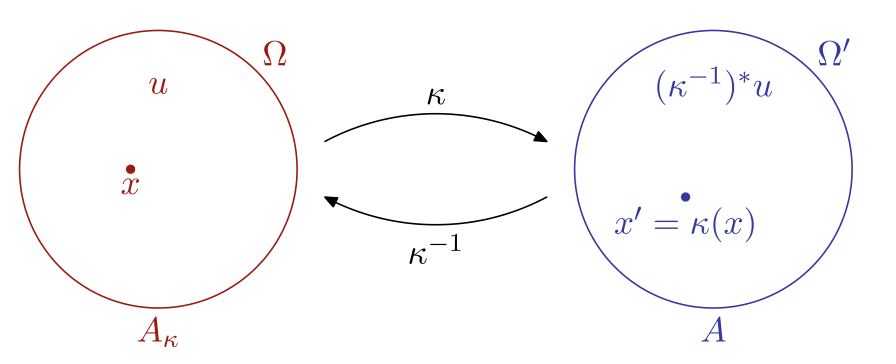
\includegraphics[width=0.72\textwidth]{figs/fig5_1_clean.png}
    \caption{伪微分算子在局部微分同胚坐标变换下的拉回几何示意.}
    \label{fig:5.1}
\end{figure}

\begin{proof}[定理~\ref{thm:5.2} 的证明]
将 $A$ 写为左量化 $A = \Op_L(a)$, 其中 $a \in S^m(\R^n; \R^n)$. 选取 $\psi \in \SmoothComp(\Omega')$ 使得在 $\supp K_A$ 上 $\psi(x) \psi(y) = 1$; 从而 $K_A(x, y) = \psi(x) K_A(x, y) \psi(y)$, 因此
\begin{equation}\label{eq:5.3}
    A = \Op\left( \psi(x) a(x, \xi) \psi(y) \right).
\end{equation}
我们在对角线附近进行局部化: 对待定的充分小常数 $\epsilon > 0$, 选取 $\chi_\epsilon(x, y) \in \Smooth(\R^{2n})$ 满足: 当 $|x - y| < \epsilon$ 时 $\chi_\epsilon(x, y) = 1$, 而当 $|x - y| > 2\epsilon$ 时 $\chi_\epsilon(x, y) = 0$. 则
\begin{equation}\label{eq:5.4}
    K_{A_\epsilon} \defeq \Op(a_\epsilon), \qquad a_\epsilon(x, y, \xi) \defeq \chi_\epsilon(x, y) \psi(x) \psi(y) a(x, \xi),
\end{equation}
是某个算子 $A_\epsilon \in \Psi_{\mathrm{c}}^m(\Omega')$ 的 Schwartz 核. 差算子
\begin{equation}\label{eq:5.5}
    R_\epsilon \defeq A - A_\epsilon
\end{equation}
是 Schwartz 核支集完全位于对角线外部的伪微分算子, 从而 $R_\epsilon \in \Psi^{-\infty}(\R^n)$, 并且其 Schwartz 核满足 $K_{R_\epsilon} \in \SmoothComp(\Omega' \times \Omega')$. 我们随后有
\begin{equation}\label{eq:5.6}
    \begin{aligned}
        (R_\epsilon)_\kappa u(x) &= \int_{\Omega'} K_{R_\epsilon}(\kappa(x), y') u(\kappa^{-1}(y')) \,\dd y' \\
        &= \int_\Omega K_{R_\epsilon}(\kappa(x), \kappa(y)) |\!\det \kappa'(y)| u(y) \,\dd y.
    \end{aligned}
\end{equation}
因此, $(R_\epsilon)_\kappa$ 的 Schwartz 核在 $x, y \in \Omega$ 时等于 $K_{R_\epsilon}(\kappa(x), \kappa(y)) |\!\det \kappa'(y)|$, 在其余位置为 0. 从而 $(R_\epsilon)_\kappa \in \Psi_{\mathrm{c}}^{-\infty}(\Omega)$.

现在只需证明 $(A_\epsilon)_\kappa \in \Psi_{\mathrm{c}}^m(\Omega)$. 首先假定 $a \in S^{-\infty}(\R^n; \R^n)$. 则
\begin{equation}\label{eq:5.7}
    \begin{aligned}
        (A_\epsilon)_\kappa u(x) &= (2\pi)^{-n} \iint_{\R^n \times \Omega'} \ee^{\ii (\kappa(x) - y') \cdot \xi'} a_\epsilon(\kappa(x), y', \xi') u(\kappa^{-1}(y')) \,\dd y' \,\dd\xi' \\
        &= (2\pi)^{-n} \iint_{\R^n \times \Omega} \ee^{\ii (\kappa(x) - \kappa(y)) \cdot \xi'} a_\epsilon(\kappa(x), \kappa(y), \xi') |\!\det \kappa'(y)| u(y) \,\dd y \,\dd\xi',
    \end{aligned}
\end{equation}
因此 $(A_\epsilon)_\kappa$ 的 Schwartz 核为
\begin{equation}\label{eq:5.8}
    \begin{aligned}
        K_{(A_\epsilon)_\kappa}(x, y) &= (2\pi)^{-n} \int_{\R^n} \ee^{\ii (\kappa(x) - \kappa(y)) \cdot \xi'} b_\epsilon(x, y, \xi') \,\dd\xi', \\
        b_\epsilon(x, y, \xi') &\defeq a_\epsilon(\kappa(x), \kappa(y), \xi') |\!\det \kappa'(y)| \\
        &= \chi_\epsilon(\kappa(x), \kappa(y)) \psi(\kappa(x)) \psi(\kappa(y)) a(\kappa(x), \xi') |\!\det \kappa'(y)|.
    \end{aligned}
\end{equation}
为了将 $K_{(A_\epsilon)_\kappa}$ 识别为伪微分算子的 Schwartz 核, 我们使用著名的 \textbf{Kuranishi 技巧} (Kuranishi trick). 将指数进行 Taylor 积分展开: 记 $\kappa_j$ 为 $\kappa$ 的第 $j$ 个分量, 我们有
\begin{equation}\label{eq:5.9}
    \kappa_j(x) - \kappa_j(y) = \sum_{k=1}^n \Phi_{jk}(x, y) (x_k - y_k), \qquad \Phi_{jk}(x, y) \defeq \int_0^1 \partial_{x_k} \kappa_j(y + t(x - y)) \,\dd t,
\end{equation}
从而有内积恒等式:
\begin{equation}\label{eq:5.10}
    (\kappa(x) - \kappa(y)) \cdot \xi' = \langle \Phi(x, y) (x - y), \xi' \rangle = \langle x - y, \Phi(x, y)^T \xi' \rangle,
\end{equation}
其中 $\Phi(x, y) = (\Phi_{jk}(x, y))_{j, k=1, \ldots, n}$, 且 $\langle \cdot, \cdot \rangle$ 为 $\R^n$ 上的标准内积. 注意到在对角线上
\begin{equation}\label{eq:5.11}
    \Phi(x, x) = \kappa'(x)
\end{equation}
处处可逆 (因为 $\kappa$ 为微分同胚). 在紧支撑集
\begin{equation}\label{eq:5.12}
    (x, y) \in \supp\left( \chi_\epsilon(\kappa(x), \kappa(y)) \psi(\kappa(x)) \psi(\kappa(y)) \right) \subset \kappa^{-1}(\supp\psi) \times \kappa^{-1}(\supp\psi) \subset \Omega \times \Omega
\end{equation}
上, 当 $\epsilon > 0$ 充分小时满足 $|\kappa(x) - \kappa(y)| \le 2\epsilon$, 从而矩阵 $\Phi(x, y)$ 在该区域内处处一致可逆. 在式~\eqref{eq:5.8} 中做线性变量代换 $\xi = \Phi(x, y)^T \xi'$, 即 $\xi' = (\Phi(x, y)^T)^{-1} \xi$, 得到
\begin{equation}\label{eq:5.13}
    \begin{aligned}
        (A_\epsilon)_\kappa &= \Op(c_\epsilon), \\
        c_\epsilon(x, y, \xi) &\defeq b_\epsilon\left( x, y, (\Phi(x, y)^T)^{-1} \xi \right) |\!\det \Phi(x, y)|^{-1} \\
        &= a_\epsilon\left( \kappa(x), \kappa(y), (\Phi(x, y)^T)^{-1} \xi \right) |\!\det \Phi(x, y)|^{-1} |\!\det \kappa'(y)|.
    \end{aligned}
\end{equation}
我们断言 $c_\epsilon \in S^{-\infty}(\R^n \times \R^n; \R^n)$; 更一般地, 若 $a \in S^m(\R^n; \R^n)$, 则由式~\eqref{eq:5.13} 定义的符号 $c_\epsilon$ 属于 $S^m(\R^n \times \R^n; \R^n)$ 且连续依赖于 $a$. 忽略平滑的 Jacobi 行列式因子, 直接微分计算可知:
\begin{equation}\label{eq:5.14}
    \begin{aligned}
        &\partial_x^\alpha \partial_y^\beta \partial_\xi^\gamma \left( a_\epsilon\left( \kappa(x), \kappa(y), (\Phi(x, y)^T)^{-1} \xi \right) \right) \\
        &= \sum_{\substack{|\alpha'| + |\alpha''| \le |\alpha| \\ |\beta'| + |\beta''| \le |\beta|}} F_{\alpha \alpha' \alpha'' \gamma}^{\beta \beta' \beta''}(x, y) \xi^{\alpha'' + \beta''} (\partial_x^{\alpha'} \partial_y^{\beta'} \partial_\xi^{\gamma + \alpha'' + \beta''} a_\epsilon)\left( \kappa(x), \kappa(y), (\Phi(x, y)^T)^{-1} \xi \right),
    \end{aligned}
\end{equation}
其中 $F_{\alpha \alpha' \alpha'' \gamma}^{\beta \beta' \beta''} \in \SmoothComp(\Omega \times \Omega)$ 仅依赖于 $\kappa$. 由于 $\Phi(x, y)^T$ 及其逆在 $\supp a_\epsilon$ 上一致有界, 存在常数 $c, C > 0$ 使得在 $\supp a_\epsilon$ 上有 $c |\xi| \le |(\Phi(x, y)^T)^{-1} \xi| \le C |\xi|$. 因此式~\eqref{eq:5.14} 被 $\langle \xi \rangle^{m - |\gamma|}$ 乘以 $a$ 的一个连续半范数所界, 正合所需. 最后, 给定 $a \in S^m(\R^n; \R^n)$, 我们选取 $a^{(j)} \in S^{-\infty}(\R^n; \R^n)$ ($j \in \N$), 它们在 $S^m(\R^n; \R^n)$ 中一致有界, 且当 $j \to \infty$ 时在 $S^{m+1}(\R^n; \R^n)$ 中收敛到 $a$. 于是相应的符号 $c_\epsilon^{(j)}$ 在 $S^m(\R^n \times \R^n; \R^n)$ 中一致有界, 并在 $S^{m+1}(\R^n \times \R^n; \R^n)$ 中收敛到 $c_\epsilon$. 令 $A_\epsilon^{(j)} = \Op(a_\epsilon^{(j)})$, 其中 $a_\epsilon^{(j)}$ 按式~\eqref{eq:5.4} 由 $a^{(j)}$ 定义, 则对所有 $u \in \SmoothComp(\R^n)$ 有 $(A_\epsilon)_\kappa u = \lim_{j \to \infty} (A_\epsilon^{(j)})_\kappa u$; 又由式~\eqref{eq:4.24}, 当 $j \to \infty$ 时 $(A_\epsilon^{(j)})_\kappa u = \Op(c_\epsilon^{(j)}) u \to \Op(c_\epsilon) u$, 从而我们在一般情形下确立了式~\eqref{eq:5.13}.

关于主符号, 我们有 $\sigma_m(A_\kappa) = \sigma_m((A_\epsilon)_\kappa) = \sigma_m(\Op(c_\epsilon))$, 它可以从约化公式~\eqref{eq:4.50} 的 (首项) 读出: 利用式~\eqref{eq:5.11}, 它由 $S^m(\R^n; \R^n) / S^{m-1}(\R^n; \R^n)$ 中的下述等价类给出:
\[
    c_\epsilon(x, x, \xi) = b_\epsilon\left( x, x, (\kappa'(x)^T)^{-1} \xi \right) |\!\det \kappa'(x)|^{-1} = a_\epsilon\left( \kappa(x), \kappa(x), (\kappa'(x)^T)^{-1} \xi \right) = a\left( \kappa(x), (\kappa'(x)^T)^{-1} \xi \right).
\]
证明完成.
\end{proof}

\section{流形, 光滑函数, 丛与密度}\label{sec:5.2}
\index{guanghua liuxing@光滑流形 (smooth manifolds)}%
\index{xiangliangcong@向量丛 (vector bundles)}%
\index{miducong@密度丛 (density bundles)}%

我们回顾:

\begin{definition}[光滑流形]\label{def:5.3}
设 $n \in \N$. 一个 $n$ 维\textbf{光滑流形} (smooth manifold) 是一个第二可数的 Hausdorff 拓扑空间 $M$, 满足:
\begin{enumerate}
    \item 对每个点 $p \in M$, 存在开邻域 $U_p \ni p$ 以及同胚映射 $F_p \colon U_p \to B(0, 1) = \{x \in \R^n : |x| < 1\} \subset \R^n$.
    \item 对所有满足 $U_p \cap U_q \neq \emptyset$ 的 $p, q \in M$, 转移映射
    \begin{equation}\label{eq:5.15}
        F_p \circ F_q^{-1}|_{F_q(U_p \cap U_q)} \colon F_q(U_p \cap U_q) \to F_p(U_p \cap U_q)
    \end{equation}
    是 $\R^n$ 开子集之间的光滑映射.
\end{enumerate}
\end{definition}

\begin{definition}[光滑结构与图册]\label{def:5.4}
设 $M$ 为光滑流形. $M$ 上的一个\textbf{图册} (atlas) 是坐标对集合 $\{(U_\alpha, F_\alpha)\}$ (其中 $M = \bigcup_\alpha U_\alpha$), 使得每个 $F_\alpha \colon U_\alpha \to F_\alpha(U_\alpha) \subset \R^n$ 均为微分同胚. 具有``任何其他图册都包含于其中''这一性质的图册称为\textbf{极大图册}, 或\textbf{光滑结构}. 极大图册中的每一个元素对 $(U, F)$ 称为一个 (局部坐标) \textbf{卡} (chart).
\end{definition}

在任意给定的光滑流形上, 始终存在唯一的极大图册. 我们还将遇到带边流形 (manifold with boundary) 以及更一般的带角柄流形 (manifold with corners): 它们的定义完全类似, 区别仅在于局部坐标卡映入 $\R^n$ 或 $[0, \infty) \times \R^{n-1}$ (对于带边流形), 以及 $[0, \infty)^k \times \R^{n-k}$ ($k \in \{0, \ldots, n\}$ 依赖于点 $p \in M$, 对应带角柄流形). 给定光滑流形 $M$, 其带角柄光滑子流形 $\Omega \subset M$ 是指满足对所有 $p \in \Omega$, 均存在局部坐标卡 $F \colon U \to F(U) \subset \R^n$ 使得
\begin{equation}\label{eq:5.16}
    \Omega \cap U = F^{-1}\left( [0, \infty)^k \times \R^{n-k} \right);
\end{equation}
带边光滑子流形正是仅允许 $k = 0, 1$ 的特例.

对 $k \in \N_0 \cup \{\infty\}$, 我们用 $\mathcal{C}^k(M)$ 表示所有满足在每个局部坐标卡下 $f \circ F_p^{-1} \in \mathcal{C}^k(B(0, 1))$ 的连续函数空间. 我们为 $\mathcal{C}^k(M)$ 配备标准的局部凸拓扑: 对于 $\Omega = B(0, 1) \subset \R^n$, $\mathcal{C}^k(\Omega)$ 通过紧集穷竭序列 $\Omega = \bigcup_{i=1}^\infty K_i$ ($K_1 \subset K_2 \subset \cdots, K_i \subset K_{i+1}^\circ$) 上的半范数族赋予 Fréchet 空间结构:
\begin{equation}\label{eq:5.17}
    |u|_{i, k} \defeq \max_{|\alpha| \le k} \max_{x \in K_i} |\partial^\alpha u(x)|.
\end{equation}
若改用半范数 $|\cdot|_{i, k}$ ($i \in \N$, $k \in \N_0$), 则 $\mathcal{C}^\infty(\Omega)$ 也成为 Fr\'echet 空间. 固定可数点集 $\{p_j\}$ 使得 $M = \bigcup_j U_{p_j}$, 我们随后用函数 $f \circ F_{p_j}^{-1} \in \mathcal{C}^k(B(0, 1))$ 的 $\mathcal{C}^k(B(0, 1))$-半范数来定义 $\mathcal{C}^k(M)$ 上的半范数.

对于紧支函数空间 $\mathcal{C}_{\mathrm{c}}^k(M)$, 首先对紧集 $K \subset M$ 定义 Fréchet 空间
\begin{equation}\label{eq:5.18}
    \dot{\mathcal{C}}^k(K) \defeq \left\{ u \in \mathcal{C}^k(M) : \supp u \subset K \right\}.
\end{equation}
现取 $M$ 的任一紧集穷竭 $M = \bigcup_{i=1}^\infty K_i$. 则 $\mathcal{C}_{\mathrm{c}}^k(M) = \bigcup_i \dot{\mathcal{C}}^k(K_i)$ 承载归纳极限拓扑, 参见 \cite[第~V.4~章]{RS72}. 它可以具体地定义如下. 取 $\phi_i \in \SmoothComp(K_{i+1}^\circ)$ 在 $K_i$ 附近等于 1, 并令 $\phi_0 \defeq 0$. 则 $\psi_i \defeq \phi_i - \phi_{i-1} \in \SmoothComp(K_{i+1}^\circ \setminus K_{i-1})$, 且在 $M$ 上 $\sum_i \psi_i = 1$. $\mathcal{C}_{\mathrm{c}}^k(M)$ 上的拓扑随后由半范数族
\begin{equation}\label{eq:5.19}
    |u|_{(w_i), (p_i)} \defeq \sup_{i} w_i p_i(\psi_i u)
\end{equation}
所生成, 其中 $(w_i)_{i \in \N}$ 为正实数列, $p_i$ 为 $\dot{\mathcal{C}}^k(K_{i+1} \setminus K_{i-1}^\circ)$ 上的连续半范数, $\sum_i \psi_i = 1$ 为从属单位分解 (详见习题~\ref{ex:5.1}--\ref{ex:5.3}).

向量丛的``实操''定义如下.

\begin{definition}[向量丛]\label{def:5.5}
设 $M$ 为 $n$ 维光滑流形. $M$ 上的实秩为 $k$ 的\textbf{实向量丛} (real vector bundle) 是一个三元组 $(\pi, E, M)$ (常记为 $\pi \colon E \to M$):
\begin{enumerate}
    \item $E$ 为 $(n+k)$ 维光滑流形, 且投影映射 $\pi \colon E \to M$ 光滑.
    \item 对任意 $p \in M$, 存在开邻域 $U_p \subset M$ 以及微分同胚 $\tau_p \colon \pi^{-1}(U_p) \to U_p \times \R^k$ 使得 $\pi(\tau_p^{-1}(q, v)) = q$.
    \item 对一切满足 $U_p \cap U_q \neq \emptyset$ 的 $p, q \in M$, 转移映射
    \begin{equation}\label{eq:5.20}
        \tau_{pq} \defeq \tau_p \circ \tau_q^{-1}|_{(U_p \cap U_q) \times \R^k} \colon (U_p \cap U_q) \times \R^k \to (U_p \cap U_q) \times \R^k
    \end{equation}
    具有形式 $\tau_{pq}(r, v) = (r, \Phi_{pq}(r) v)$, 其中 $\Phi_{pq} \colon U_p \cap U_q \to \mathrm{GL}(k)$ 是光滑映射.
\end{enumerate}
点 $p \in M$ 上的纤维记作 $E_p \defeq \pi^{-1}(p)$; 它具有实 $k$ 维向量空间的结构. $E$ 的零截面 $o$ 是 $E$ 的子流形, 在 $\pi^{-1}(U_p)$ 内局部地由 $\tau_p^{-1}(U_p \times \{0\})$ 给出. $E$ 的光滑截面是满足 $\pi \circ s = \operatorname{Id}_M$ 的光滑映射 $s \colon M \to E$; 光滑截面空间记作 $\mathcal{C}^\infty(M; E)$. 将 $\R^k$ 替换为 $\mathbb{C}^k$ 即得到\textbf{复向量丛}.

我们称映射 $\tau_p$ 为\emph{局部平凡化}. 若 $U_p$ 是坐标卡 $F \colon U_p \to F(U_p) \subset \R^n$ 的定义域, 则也称 $(F \times \operatorname{Id}) \circ \tau_p \colon \pi^{-1}(U_p) \to F(U_p) \times \R^k$ 为局部平凡化.
\end{definition}

\begin{definition}[纤维丛]\label{def:5.6}
设 $M$ 为 $n$ 维光滑流形; $F$ 为 $k$ 维光滑流形. 典型纤维为 $F$ 的\textbf{纤维丛} (fiber bundle) 是三元组 $(\pi, E, M)$, 具有如下性质:
\begin{enumerate}
    \item $E$ 为 $(n+k)$ 维光滑流形, 且投影映射 $\pi \colon E \to M$ 光滑.
    \item 对任意 $p \in M$, 存在开邻域 $U_p \subset M$ ($p \in U_p$) 以及微分同胚 $\tau_p \colon \pi^{-1}(U_p) \to U_p \times F$ 使得 $\pi(\tau_p^{-1}(q, f)) = q$.
    \item 对一切满足 $U_p \cap U_q \neq \emptyset$ 的 $p, q \in M$, 转移映射
    \begin{equation}\label{eq:5.21}
        \tau_{pq} \defeq \tau_p \circ \tau_q^{-1}|_{(U_p \cap U_q) \times F} \colon (U_p \cap U_q) \times F \to (U_p \cap U_q) \times F
    \end{equation}
    具有形式 $\tau_{pq}(r, f) = (r, \Phi_{pq}(r, f))$, 其中对每个 $r \in U_p \cap U_q$, $\Phi_{pq}(r, \cdot) \colon F \to F$ 是微分同胚.
\end{enumerate}
\end{definition}

回到向量丛. 注意: 为了唯一确定 (在同构意义下) 一个实秩 $k$ 向量丛, 只需具备如下数据与条件:
\begin{enumerate}
    \item $M$ 的一个由非空开子集组成的覆盖 $\{U_\alpha\}$.
    \item 对一切满足 $U_{\alpha\beta} \defeq U_\alpha \cap U_\beta \neq \emptyset$ 的 $\alpha, \beta$, 一个形如 $\tau_{\alpha\beta}(p, v) = (p, \Phi_{\alpha\beta}(p) v)$ 的映射 $\tau_{\alpha\beta} \colon U_{\alpha\beta} \times \R^k \to U_{\alpha\beta} \times \R^k$, 其中 $\Phi_{\alpha\beta} \colon U_{\alpha\beta} \to \mathrm{GL}(k)$ 光滑.
    \item 对一切 $p \in U_\alpha$, $v \in \R^k$ 有 $\tau_{\alpha\alpha}(p, v) = (p, v)$.
    \item 循环条件成立: 对满足 $U_{\alpha\beta\gamma} \defeq U_\alpha \cap U_\beta \cap U_\gamma \neq \emptyset$ 的 $\alpha, \beta, \gamma$, 在 $U_{\alpha\beta\gamma} \times \R^k$ 上有 $\tau_{\gamma\beta} \circ \tau_{\beta\alpha} = \tau_{\gamma\alpha}$.
\end{enumerate}
事实上, 此时可以令
\begin{equation}\label{eq:5.22}
    E \defeq \left( \bigsqcup_\alpha U_\alpha \times \R^k \right) / \sim
\end{equation}
唯一构筑向量丛, 其中等价关系 $\sim$ 定义为
\begin{equation}\label{eq:5.23}
    U_\alpha \times \R^k \ni (p, v) \sim (q, w) \in U_\beta \times \R^k \iff p = q, \ \tau_{\alpha\beta}(q, w) = (p, v).
\end{equation}
(循环条件保证该关系具有传递性, 而自反性由循环条件连同 $\tau_{\alpha\alpha} = \mathrm{Id}$ 推出.) 我们用 $[U_\alpha, (p, v)] \in E$ 表示等价类. 注意同一点 $p$ 可以落在两个 (或更多) 开集 $U_\alpha$ 与 $U_\beta$ 中, 但对 $v \in \R^k$ 通常有 $[U_\alpha, (p, v)] \neq [U_\beta, (p, v)]$. 投影映射 $\pi \colon E \to M$ 简单地由 $\pi([U_\alpha, (p, v)]) = p$ 给出. 作为局部平凡化, 我们可以取:
\begin{equation}\label{eq:5.24}
    \tau_\alpha \colon \{ [U_\alpha, (p, v)] : p \in U_\alpha \} \to U_\alpha \times \R^k, \qquad [U_\alpha, (p, v)] \mapsto (p, v).
\end{equation}

\begin{example}[切丛与余切丛]\label{eg:5.7}
取 $n$ 维流形 $M$ 由坐标卡 $F_i \colon U_i \to \R^n$ 构成的覆盖, 考虑 $\tau_{ij}(p, v) = (p, (F_i \circ F_j^{-1})'|_{F_j(p)} v)$. 所得的向量丛是 $M$ 的\textbf{切丛}, 记作 $TM$. 注意一个坐标卡 $F \colon U \to \R^n$ 通过 $U \times \R^n \ni (p, v) \mapsto [U, (p, v)] \in T_U M$ 诱导出 $T_U M \defeq \pi^{-1}(U)$ 的一个平凡化. (为最大精确起见, 人们不仅应记录 $U$, 还应记录 $F$, 即写 $[U, F, (p, v)] \in T_U M$.) 切向量 $V = [U, (p, v)] \in T_p M$ 具有方向导数的解释:
\begin{equation}\label{eq:5.25}
    \mathcal{C}^\infty(M) \ni f \mapsto V(f) \defeq \left. \frac{\dd}{\dd s} \left( ((F^{-1})^* f|_U)(F(p) + s v) \right) \right|_{s = 0}.
\end{equation}
(亦见习题~\ref{ex:5.4}.)

(2) $V$ 是 $M$ 上一条光滑曲线的切向量. 这来自如下构造: 考虑所有满足 $\gamma(0) = p$ 的光滑曲线 $\gamma \colon I \to M$ 的集合, 其中 $I \subset \R$ 是含 0 的开区间. 在该集合上定义等价关系如下: $\gamma_1 \sim \gamma_2$ 当且仅当在任一满足 $p \in U$ 的局部坐标系 $F \colon U \to \R^n$ 中, 有 $\frac{\dd}{\dd s} F(\gamma_1(s))|_{s = 0} = \frac{\dd}{\dd s} F(\gamma_2(s))|_{s = 0}$. (请验证该条件与 $F$ 的选取无关.) 于是 $T_p M$ 就是曲线的等价类的集合, 而切向量 $V$ 等同于曲线 $s \mapsto F^{-1}(F(p) + s v)$ 所在的等价类.

向量空间上的函子性运算给出向量丛上相应的运算. 例如, 给定两个向量空间之间的线性映射 $A \colon V \to W$, 其伴随为 $A^T \colon W^* \to V^*$; 若 $A$ 可逆, 则这给出映射 $(A^T)^{-1} \colon V^* \to W^*$. 于是在例~\ref{eg:5.7} 的记号下, 我们可以取
\begin{equation}\label{eq:5.26}
    \tau_{ij}(p, v) \defeq \left( p, \left( (\kappa_{ij}'|_{F_j(p)})^T \right)^{-1} v \right), \qquad \kappa_{ij} \defeq F_i \circ F_j^{-1},
\end{equation}
所得的向量丛是余切丛, 记作 $\pi \colon T^* M \to M$. 注意公式~\eqref{eq:5.26} 已经在 式~\eqref{eq:5.2} 中出现过 (只是在后者中我们还通过 $\kappa_{ij}$ 更换了底空间 $M$ 上的局部坐标). 对任意光滑函数 $f \in \mathcal{C}^\infty(M)$, 其外微分 $\dd f$ 在每个坐标卡下定义为
\begin{equation}\label{eq:5.27}
    \tau_i(\dd f(p)) \defeq \left( p, (\partial_{x_j}((F_i^{-1})^* f))_{j=1, \ldots, n} \right) \in U_i \times \R^n, \qquad p \in U_i;
\end{equation}
这确实给出 $T^* M$ 的一个良定义的截面, 这一点由变量变换公式推出. 与例~\ref{eg:5.7} 中一样, 局部坐标系 $F \colon U \to \R^n$ 诱导出平凡化 $T^* U = \pi^{-1}(U) \cong U \times \R^n$; $\R^n$ 因子上的标准坐标称为\textbf{典范动量变量} (canonical momentum variables). $T^* M$ 与 $TM$ 之间的关系如下: 对任意 $p \in M$, 我们有向量空间的同构
\begin{equation}\label{eq:5.28}
    T_p^* M \cong \operatorname{Hom}(T_p M, \R)
\end{equation}
它不依赖于任何选取. 该同构可在由同一局部坐标系 $F$ 诱导的 $TM$ 与 $T^* M$ 的局部平凡化中描述如下: 若 $\omega = [U, (p, \xi)] \in T_p^* M$ 且 $V = [U, (p, v)] \in T_p M$, 其中 $\xi, v \in \R^n$, 则令 $\omega(V) = \langle \xi, v \rangle$ (欧氏内积). 见习题~\ref{ex:5.5}.

在 $p$ 附近的坐标卡 $F_i$ 中, $f$ 的一个自然取法是 $f = F_i^* x_k$ (当坐标卡从上下文看很清楚时也写作 $f = x_k$); 此时式~\eqref{eq:5.27} 定义了微分 $\dd x_k$, 满足 $\tau_i(\dd x_k) = (p, (0, \ldots, 1, \ldots, 0))$ (1 位于第 $k$ 个位置). 外微分 $\dd f$ 则通常写作 $\dd f = \sum_{j=1}^n (\partial_{x_j} f) \dd x^j$ (即在记号中略去坐标映射与平凡化映射).
\end{example}

\begin{example}[向量丛上的代数运算]\label{eg:5.8}
设 $E, F \to M$ 为向量丛.
\begin{enumerate}
    \item 逐纤维直和产生直和丛 $E \oplus F \to M$, 其纤维为 $(E \oplus F)_p = E_p \oplus F_p$.
    \item 逐纤维张量积产生张量积丛 $E \otimes F \to M$, 其纤维为 $(E \otimes F)_p = E_p \otimes F_p$.
    \item 同态丛 $\Hom(E, F) \to M$ 的纤维为 $\Hom(E_p, F_p)$, 且有自然等同 $\Hom(E, F) = E^* \otimes F$.
    \item 设 $q \in \N$. 逐纤维取 $q$ 次外积幂产生向量丛 $\Lambda^q E \to M$. 在 $E = T^* M$ 的特例中, 人们常写 $\Lambda^q M \defeq \Lambda^q T^* M$.
\end{enumerate}
\end{example}

向量丛上另一个有用的运算如下.

\begin{definition}[拉回向量丛]\label{def:5.9}
设 $M$, $N$ 为光滑流形 (不要求维数相同), 且 $f \colon M \to N$ 光滑. 若 $\pi \colon E \to N$ 为向量丛, 则 $E$ 沿 $f$ 的拉回是向量丛 \begin{equation}\label{eq:5.29}
    \tilde{\pi} \colon f^* E \to M,
\end{equation}
它由 $f^* E \defeq \left\{ (p, e) \in M \times E : f(p) = \pi(e) \right\}$ 给出, 投影映射为 $\tilde{\pi}(p, e) = p$, 且 $(f^* E)_p = E_{f(p)}$ 上的线性结构取为 $E_{f(p)}$ 上的线性结构.
\end{definition}

我们接下来引入一个重要的向量丛, 它与 $n$ 维流形 $M$ 的余切丛的最高外积幂 $\Lambda^n T^* M$ 密切相关:

\begin{definition}[密度丛]\label{def:5.10}
设 $M$ 为 $n$ 维光滑流形, $\alpha \in \R$. $M$ 上的 $\alpha$-\textbf{密度丛} (density bundle) 是秩为 1 的向量丛
\begin{equation}\label{eq:5.30}
    \Omega^\alpha M \to M,
\end{equation}
其转移函数为 $\tau_{ij}(p, v) = \left( p, |\!\det \kappa_{ij}'|_{F_j(p)}|^{-\alpha} v \right)$, $\kappa_{ij} = F_i \circ F_j^{-1}$. 我们还记
\begin{equation}\label{eq:5.31}
    \Omega M \defeq \Omega^1 M.
\end{equation}
由于转移函数 $\tau_{ij}$ 在第二个变量 ($v$) 上的作用是乘以一个正函数, 故存在良定义的\textbf{正 $\alpha$-密度}概念: 它们是指在 $M$ 上某个坐标卡给出的 $\Omega^\alpha M$ 平凡化下由正光滑函数表示的密度. 体积密度是指光滑的正 1-密度.
\end{definition}

\begin{remark}[密度丛的函子性视角]\label{rem:5.11}
$\Omega^\alpha M \to M$ 函子性地来自下述作用于向量空间的运算 (将它施加于 $TM$): 给定实 $n$ 维向量空间 $V$, 我们定义
\begin{equation}\label{eq:5.32}
    \Omega^\alpha V \defeq \left\{ \omega \colon \Lambda^n V \to \R : \omega(\mu v) = |\mu|^\alpha \omega(v), \ v \in \Lambda^n V, \ \mu \in \R \right\}.
\end{equation}
为看出二者关系, 先注意 $\Lambda^n V$ 是一维的. 然后, 给定另一个 $n$ 维向量空间 $W$ 以及线性映射 $\kappa \colon V \to W$, 我们取定 $V$ 的基 $e_1, \ldots, e_n$ 与 $W$ 的基 $f_1, \ldots, f_n$. 作为热身考察最高外积幂: $e_1 \wedge \cdots \wedge e_n$ 与 $f_1 \wedge \cdots \wedge f_n$ 分别是 $\Lambda^n V$ 与 $\Lambda^n W$ 的基, 而映射 $\Lambda^n \kappa \colon \Lambda^n V \to \Lambda^n W$ 由
\begin{equation}\label{eq:5.33}
    \Lambda^n \kappa \colon e_1 \wedge \cdots \wedge e_n \mapsto \kappa(e_1) \wedge \cdots \wedge \kappa(e_n) = (\det \kappa) f_1 \wedge \cdots \wedge f_n
\end{equation}
给出, 其中 $\det \kappa$ 是 $\kappa$ 在这两组基下的矩阵的行列式. 类似地, $\Omega^\alpha V$ 与 $\Omega^\alpha W$ 都是一维的, 其基元素分别为 $\omega_V \colon \mu e_1 \wedge \cdots \wedge e_n \mapsto |\mu|^\alpha$ 与 $\omega_W \colon \mu f_1 \wedge \cdots \wedge f_n \mapsto |\mu|^\alpha$. 对可逆的 $\kappa \colon V \to W$, 映射
\begin{equation}\label{eq:5.34}
    \Omega^\alpha \kappa \colon \Omega^\alpha V \to \Omega^\alpha W
\end{equation}
由下式给出:
\begin{equation}\label{eq:5.35}
    (\Omega^\alpha \kappa)(\omega)(f_1 \wedge \cdots \wedge f_n) \defeq \omega(\kappa^{-1}(f_1) \wedge \cdots \wedge \kappa^{-1}(f_n)),
\end{equation}
从而 $\Omega^\alpha \kappa(\omega_V) = |\!\det\kappa|^{-\alpha} \omega_W$.
\end{remark}

下述简单引理的证明留给读者 (习题~\ref{ex:5.9}).

\begin{lemma}[密度丛的性质]\label{lem:5.12}
设 $\alpha, \beta \in \R$. 则:
\begin{enumerate}
    \item $(\Omega^\alpha M)^* \cong \Omega^{-\alpha} M$.
    \item $\Omega^\alpha M \otimes \Omega^\beta M \cong \Omega^{\alpha+\beta} M$.
    \item $\Omega^0 M \cong M \times \R$.
\end{enumerate}
\end{lemma}

若 $x \in \R^n$ 表示流形 $M$ 上的局部坐标, 则一个典型的 $\alpha$-密度为
\begin{equation}\label{eq:5.36}
    |\dd x|^\alpha \colon \mu \partial_{x_1} \wedge \cdots \wedge \partial_{x_n} \mapsto |\mu|^\alpha.
\end{equation}
与微分形式类似, $\alpha$-密度可以被光滑映射拉回 (习题~\ref{ex:5.13}):

\begin{lemma}[密度的拉回]\label{lem:5.13}
设 $f \colon M \to N$ 为同维数光滑流形之间的光滑映射, 且假定 $f$ 没有临界点. 在局部坐标 $x, y$ 下, 对 $\alpha$-密度 $u(y) = u_0(y) |\dd y|^\alpha$, 定义 $(f^* u)(x) \defeq u_0(f(x)) |\!\det f'(x)|^\alpha |\dd x|^\alpha$. 则 $f^*$ 是良定义的映射:
\begin{equation}\label{eq:5.37}
    f^* \colon \Smooth(N; \Omega^\alpha N) \to \Smooth(M; \Omega^\alpha M).
\end{equation}
\end{lemma}

\begin{remark}[内蕴表述]\label{rem:5.14}
若 $V \in T_p M$, 定义其前推向量 $f_* V \in T_{f(p)} N$ 满足 $(f_* V)(g) = V(f^* g)$ ($\forall\,g \in \Smooth(N)$). 则引理~\ref{lem:5.13} 中 $\alpha$-密度的拉回内蕴地由下式给出:
\[
    (f^* u)|_p(V_1 \wedge \cdots \wedge V_n) \defeq u|_{f(p)}(f_* V_1 \wedge \cdots \wedge f_* V_n), \qquad n = \dim M.
\]
\end{remark}

\begin{proposition}[1-密度的积分]\label{prop:5.15}
对我们而言 1-密度最为有用: $\Omega M$ 的截面可以被不变地积分. 在 $\R^n$ 上, 对 $u = u_0(x) |\dd x| \in \mathcal{C}_{\mathrm{c}}^\infty(\R^n; \Omega \R^n)$, 我们记
\begin{equation}\label{eq:5.38}
    \int_{\R^n} u \defeq \int_{\R^n} u_0(x) \,\dd x.
\end{equation}
设 $\{\phi_i\}$ 为从属于开覆盖 $F_i \colon U_i \to F_i(U_i) \subset \R^n$ 的紧支单位分解. 定义全流形上的积分映射
\begin{equation}\label{eq:5.39}
    \int_M \colon \mathcal{C}_{\mathrm{c}}^\infty(M; \Omega M) \to \R, \qquad u \mapsto \sum_i \int_{\R^n} (F_i^{-1})^*(\phi_i u).
\end{equation}
(这里 $(F_i^{-1})^*(\phi_i u) \in \mathcal{C}_{\mathrm{c}}^\infty(\R^n; \Omega \R^n)$ 由引理~\ref{lem:5.13} 定义.) 映射~\eqref{eq:5.39} 与局部坐标的选取以及单位分解的选取无关.
\end{proposition}

\begin{proof}
设 $u \in \mathcal{C}_{\mathrm{c}}^\infty(M; \Omega M)$ 支撑在两个坐标卡的交集内, 局部坐标分别为 $x$ 与 $y$, 转移映射为 $x = \kappa(y)$. 此时
\begin{equation}\label{eq:5.40}
    u = u_0(x) |\dd x| = u_1(y) |\dd y|.
\end{equation}
在 $x = \kappa(y)$ 处, 我们有 $(\Omega^1 \kappa) |\dd y| = |\!\det \kappa'(y)|^{-1} |\dd x|$, 从而 $|\dd x| = |\!\det \kappa'(y)| |\dd y|$. 因此 $u_1(y) = u_0(\kappa(y)) |\!\det \kappa'(y)|$, 于是
\begin{equation}\label{eq:5.41}
    \int_{\R^n} u_1(y) \,\dd y = \int_{\R^n} u_0(\kappa(y)) |\!\det \kappa'(y)| \,\dd y = \int_{\R^n} u_0(x) \,\dd x.
\end{equation}
命题由此容易推出: 若 $\{\psi_j\}$ 是从属于由坐标系 $G_j \colon V_j \to G_j(V_j) \subset \R^n$ 构成的覆盖的另一单位分解, 则 $\int_M u = \sum_j \int_M \psi_j u$, 从而
\[
    \begin{aligned}
        \int_M u &= \sum_j \int_M \psi_j u \\
        &= \sum_{i, j} \int_{\R^n} (F_i^{-1})^*(\phi_i \psi_j u) \\
        &= \sum_{i, j} \int_{\R^n} (G_j \circ F_i^{-1})^*\left( (G_j^{-1})^*(\psi_j \phi_i u) \right) \\
        &= \sum_{i, j} \int_{\R^n} (G_j^{-1})^*(\psi_j \phi_i u) \\
        &= \sum_j \int_{\R^n} (G_j^{-1})^* \psi_j u.
    \end{aligned}
\]
证明完毕.
\end{proof}

我们现在可以定义:

\begin{definition}[流形上的分布空间]\label{def:5.16}
流形 $M$ 上的 (复数值) \textbf{分布空间} $\Distr(M)$ 由所有连续线性映射 $\mathcal{C}_{\mathrm{c}}^\infty(M; \Omega M) \to \mathbb{C}$ 组成. 更一般地, 若 $E \to M$ 为复 (或实) 向量丛, 则 $E$-\textbf{值分布空间} $\Distr(M; E)$ 由所有连续线性泛函 $\mathcal{C}_{\mathrm{c}}^\infty(M; E^* \otimes \Omega M) \to \mathbb{C}$ (或 $\R$) 组成; 空间 $\mathscr{E}'(M; E)$ 由所有连续线性泛函 $\mathcal{C}^\infty(M; E^* \otimes \Omega M) \to \mathbb{C}$ (或 $\R$) 组成.

于是 $\mathcal{C}^\infty(M; E) \hookrightarrow \Distr(M; E)$ 经由
\begin{equation}\label{eq:5.42}
    \mathcal{C}^\infty(M; E) \times \mathcal{C}_{\mathrm{c}}^\infty(M; E^* \otimes \Omega M) \ni (u, \phi) \mapsto \int_M \langle u(p), \phi(p) \rangle
\end{equation}
嵌入, 其中 $\langle \cdot, \cdot \rangle \colon E^* \times E \to \R$ 是对偶配对; 注意 $\langle u, \phi \rangle \in \mathcal{C}^\infty(M; \Omega M)$ 确实可由命题~\ref{prop:5.15} 不变地积分.
\end{definition}

线性映射 $\mathcal{C}_{\mathrm{c}}^\infty(M; \Omega M) \to \mathbb{C}$ 的连续性等价于它到每个 $\dot{\mathcal{C}}^\infty(K; \Omega M)$ ($K \subset M$ 为紧集) 上的限制都是序列连续的 (习题~\ref{ex:5.2}). 分布的支集与奇支集的定义与局部 ($\R^n$) 情形类似(定义~\ref{def:2.6}). 空间 $\mathscr{E}'(M; E) \subset \Distr(M; E)$ 是具紧支集的分布的空间. (若没有额外的结构, 在一般光滑流形上并没有 Schwartz 函数空间或缓增分布空间的自然类比.)

\begin{example}[流形上的 Dirac $\delta$-分布]\label{eg:5.17}
设 $p \in M$. 则 $\delta_p \in \mathscr{E}'(M; \Omega M)$ 定义为将测试函数 $\phi \in \mathcal{C}^\infty(M)$ 映为 $\phi(p)$. 注意这里 $\mathscr{E}'(M; \Omega M)$ 中元素的测试函数空间, 由引理~\ref{lem:5.12}, 等于丛 $(\Omega M)^* \otimes \Omega M = M \times \R$ 的光滑截面空间, 即光滑函数空间.
\end{example}

分布由它们的局部行为刻画: 线性映射 $u \colon \mathcal{C}_{\mathrm{c}}^\infty(M; \Omega M) \to \mathbb{C}$ 是分布, 当且仅当对所有坐标卡 $F \colon U \to F(U) \subset \R^n$ 以及所有光滑函数 $\chi \in \mathcal{C}_{\mathrm{c}}^\infty(F(U))$, 映射
\begin{equation}\label{eq:5.43}
    \Schwartz(\R^n) \ni \phi \mapsto \langle u, F^*(\chi \phi |\dd x|) \rangle \in \mathbb{C}
\end{equation}
定义了 $\R^n$ 上的一个 (具紧支集的) 缓增分布.

记两投影映射为: \begin{equation}\label{eq:5.44}\pi_L \colon M^2 \to M, \quad (p, q) \mapsto p, \qquad \pi_R \colon M^2 \to M, \quad (p, q) \mapsto q.\end{equation}

\begin{theorem}[Schwartz 核定理: 流形情形]\label{thm:5.18}
设 $M$ 为光滑 $n$ 维流形, $E, F \to M$ 为两个向量丛. 则在连续线性算子 $A \colon \mathcal{C}_{\mathrm{c}}^\infty(M; E) \to \Distr(M; F)$ 与分布 Schwartz 核 $K \in \Distr\left( M \times M; \pi_L^* F \otimes \pi_R^*(E^* \otimes \Omega M) \right)$ 之间存在一一对应. 该对应把 $K$ 对应到算子 $O_K \colon \mathcal{C}_{\mathrm{c}}^\infty(M; E) \to \Distr(M; F)$, 定义为
\begin{equation}\label{eq:5.45}
    (O_K \phi)(\psi) = \langle K, \pi_L^* \psi \otimes \pi_R^* \phi \rangle, \qquad \phi \in \mathcal{C}_{\mathrm{c}}^\infty(M; E), \ \psi \in \mathcal{C}_{\mathrm{c}}^\infty(M; F^* \otimes \Omega M).
\end{equation}
\end{theorem}

请读者自行给出定理~\ref{thm:5.18} 的一个推广的证明, 见习题~\ref{ex:5.15}.

\section{流形上的微分算子}\label{sec:5.3}
\index{liuxingshang weifen suanzi@流形上的微分算子 (differential operators on manifolds)}%

设 $M$ 为光滑 $n$ 维流形. 在讨论 $M$ 上的伪微分算子之前, 我们先思考微分算子.

\begin{definition}[光滑向量场空间]\label{def:5.19}
流形 $M$ 上的光滑 (实) 向量场空间为 $\mathcal{V}(M) \defeq \mathcal{C}^\infty(M; TM)$. 在 $M$ 上的局部坐标 $x_1, \ldots, x_n$ 中, 每个 $V \in \mathcal{V}(M)$ 都可写成 $V = \sum_{j=1}^n V_j(x) \partial_{x_j}$ 的形式, 其中 $V_j$ ($j = 1, \ldots, n$) 是光滑实值函数. 我们也会遇到复向量场: 它在局部坐标下具有同样的形式, 但 $V_j$ 取复值. (等价地, 复向量场是复化切丛 $\mathbb{C} \otimes TM$ 的截面.)

一个元素 $V \in \mathcal{V}(M)$ 可以通过令
\begin{equation}\label{eq:5.46}
    \mathcal{C}^\infty(M) \ni f \mapsto V f \in \mathcal{C}^\infty(M), \qquad (V f)(p) = \dd f(p)(V(p))
\end{equation}
而视为一个微分算子.
\end{definition}

\begin{definition}[流形上的微分算子代数]\label{def:5.20}
\begin{enumerate}
    \item $\Diff^0(M) \defeq \mathcal{C}^\infty(M)$, 作用为逐点函数乘法.
    \item $\Diff^1(M)$ 由所有形如 $A u = V u + f u$ ($V \in \mathcal{V}(M), f \in \mathcal{C}^\infty(M)$) 的算子组成.
    \item 设 $m \in \N_0$. 则 $\Diff^m(M)$ 是所有算子 $A \colon \SmoothComp(M) \to \SmoothComp(M)$ 的空间, 使得对任意紧子集 $K \subset M$, 存在 $N \in \N$ 以及 $A_{kj} \in \Diff^1(M)$ ($k = 1, \ldots, N$, $j = 1, \ldots, N_k \le m$) 满足
    \begin{equation}\label{eq:5.47}
        \begin{aligned}
            A u &= \sum_{k=1}^N A_{k1} \cdots A_{kN_k} u, \qquad \forall\, u \in \dot{\mathcal{C}}^\infty(K), \\
            \dot{\mathcal{C}}^\infty(K) &\defeq \left\{ u \in \mathcal{C}^\infty(M) : \supp u \subset K \right\}.
        \end{aligned}
    \end{equation}
\end{enumerate}
\end{definition}

(请验证这与标准局部坐标定义一致.) 当然, 微分算子也把 $\mathcal{C}^\infty(M)$ 映到 $\mathcal{C}^\infty(M)$, 把 $\Distr(M)$ 映到 $\Distr(M)$, 把 $\mathscr{E}'(M)$ 映到 $\mathscr{E}'(M)$.

微分算子的 Schwartz 核是什么? 恒等算子 $I \in \Diff^0(M)$ 的 Schwartz 核 $K_I$ 应当是
\begin{equation}\label{eq:5.48}
    K_I(x, y) = \delta(x - y).
\end{equation}
我们的目标是使这一点有意义. 利用式~\eqref{eq:5.44} 中的右投影 $\pi_R$, 我们定义\textbf{右密度丛}为
\begin{equation}\label{eq:5.49}
    \Omega_R \defeq \pi_R^*(\Omega M) \to M \times M.
\end{equation}
于是, 在第二个变量中积分是一个良定义的映射 $\SmoothComp(M^2; \Omega_R) \to \SmoothComp(M)$. 更一般地, 下述映射是良定义的:
\begin{equation}\label{eq:5.50}
    \Distr(M^2; \Omega_R) \times \SmoothComp(M) \ni (K, u) \mapsto \int_M K(\cdot, y) u(y) \in \Distr(M).
\end{equation}
由 Schwartz 核定理, 每一个连续线性映射 $\SmoothComp(M) \to \Distr(M)$ 均由某个 $K \in \Distr(M^2; \Omega_R)$ 所表示. 因此, 式~\eqref{eq:5.48} 必须被视为如下空间中的元素:
\begin{equation}\label{eq:5.51}
    K_I \in \Distr(M^2; \Omega_R).
\end{equation}
作为该类分布, 它作用在如下检验函数类上:
\begin{equation}\label{eq:5.52}
    \SmoothComp(M^2; \Omega(M^2) \otimes (\Omega_R)^*) = \SmoothComp(M^2; \Omega_L), \qquad \Omega_L \defeq \pi_L^*(\Omega M),
\end{equation}
并且确实把 $u \in \SmoothComp(M^2; \Omega_L)$ 映为由命题~\ref{prop:5.15} 定义的 $\int_M u(x, x)$. 这里我们用到 $\Omega(M^2) = \Omega_L \otimes \Omega_R$; 此外还用到 $(\Omega_L)_{(x, y)} = \Omega_x M$, 从而限制到对角线定义了一个映射 $\SmoothComp(M^2; \Omega_L) \to \SmoothComp(M; \Omega M)$.

给定 $A \in \Diff^m(M)$, 其 Schwartz 核 $K_A \in \Distr(M^2; \Omega_R)$ 随后由
\begin{equation}\label{eq:5.53}
    K_A = (\pi_L^* A) K_I \in \Distr(M^2; \Omega_R)
\end{equation}
给出, 其中 $\pi_L^* A$ 表示 $A$ 提升到第 0 个因子上. (读者应自行验证: 若 $\pi \colon E \to M$ 是向量丛且 $K \in \Distr(M^2; \pi_R^* E)$, 则下述式子良定义——这里 $K(\cdot, y)$ 取值于 $E_y$, 而在取定 $E_y$ 的任意与 $x$ 无关的基之后 $A$ 逐分量作用.)

更一般地, 若 $K \in \Distr(M^2; \pi_R^* E)$, 则
\begin{equation}\label{eq:5.54}
    (\pi_L^* A) K \in \Distr(M^2; \pi_R^* E), \qquad ((\pi_L^* A) K)(\cdot, y) \defeq A(K(\cdot, y)), \quad y \in M
\end{equation}
良定义; 在此 $K(\cdot, y)$ 取值于 $E_y$, 且在选定 $E_y$ 的任意与 $x$ 无关的基底后 $A$ 逐分量作用.

\section{流形上伪微分算子空间的定义}\label{sec:5.4}
\index{liuxingshang weifen suanzi kongjian@流形上伪微分算子空间 (pseudodifferential operators on manifolds)}%
\index{shizhengzhiji suanzi@适正支集算子 (properly supported operators)}%

我们继续用 $M$ 表示光滑 $n$ 维流形, 并使用式~\eqref{eq:5.44} 中的记号 $\pi_L$, $\pi_R$ 以及式~\eqref{eq:5.49} 中的 $\Omega_R$. 下述定义所刻画的正是我们希望流形 (不必紧致) 上的伪微分算子所是的样子: 它们的 Schwartz 核在对角线附近应当是 $\R^n$ 上伪微分算子在局部坐标下的 Schwartz 核, 而在对角线之外则应当是光滑的 (对比推论~\ref{cor:4.9}).

\begin{definition}[流形上的伪微分算子空间]\label{def:5.21}
设 $M$ 为光滑 $n$ 维流形, $m \in \R \cup \{-\infty\}$. 则 $\Psi^m(M)$ 是所有满足下列性质的线性算子
\begin{equation}\label{eq:5.55}
    A \colon \mathcal{C}_{\mathrm{c}}^\infty(M) \to \mathcal{C}^\infty(M)
\end{equation}
组成:
\begin{subequations}\label{eq:5.56}
\begin{enumerate}
    \item 若 $F \colon U \subset M \to F(U) \subset \R^n$ 是坐标卡且 $\psi \in \SmoothComp(U)$, 则存在 $B \in \Psi_{\mathrm{c}}^m(F(U)) \subset \Psi^m(\R^n)$ (见定义~\ref{def:5.1}), 使得在 $U$ 上有
    \begin{equation}\label{eq:5.56a}
        \psi A(\psi u) = F^*\left( B\left( (F^{-1})^* u \right) \right), \qquad u \in \SmoothComp(M).
    \end{equation}
    \item 若 $\phi, \psi \in \mathcal{C}^\infty(M)$ 满足 $\supp \phi \cap \supp \psi = \emptyset$, 则算子 $\phi A \psi$ 具有处处光滑的右密度核 $K \in \mathcal{C}^\infty(M^2; \Omega_R)$, 即对所有 $u \in \SmoothComp(M)$,
    \begin{equation}\label{eq:5.56b}
        \phi A (\psi u) = \int_M K(\cdot, y) u(y).
    \end{equation}
\end{enumerate}
\end{subequations}
(见图~\ref{fig:5.2}.)
\end{definition}

\begin{figure}[htbp]
    \centering
    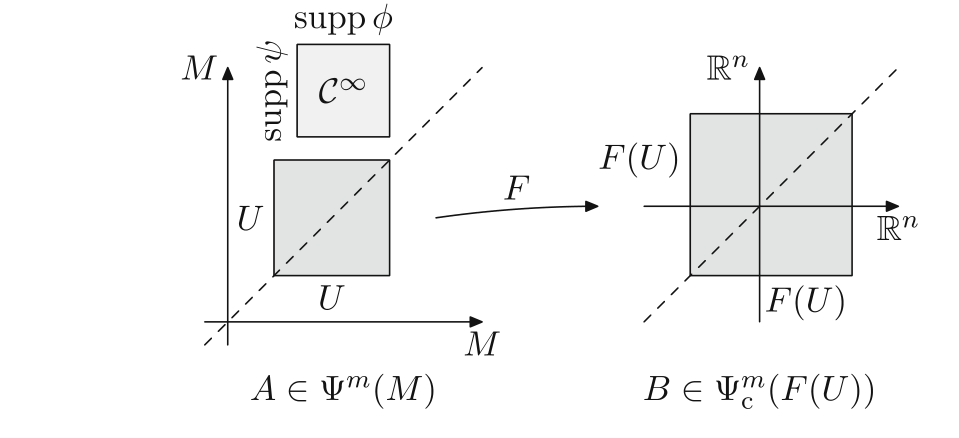
\includegraphics[width=0.72\textwidth]{figs/fig5_2_clean.png}
    \caption{流形上伪微分算子通过坐标卡局域化与对角线外光滑余核的定义分解示意.}
    \label{fig:5.2}
\end{figure}

\begin{remark}[流形 $\R^n$ 上的算子类与一致算子类的对比]\label{rem:5.22}
取光滑流形 $M = \R^n$, 则此处定义的 $\Psi^m(M)$ 远远大于第~\ref{ch:04}~章中定义的一致伪微分算子空间 $\Psi^m(\R^n)$. (一个原因是: 我们并不限制 Schwartz 核在对角线 $\operatorname{diag}_M = \{(p, p) : p \in M\}$ 之外的大小.) 为避免混淆, 后者应当记为 $\Psi_\infty^m(\R^n)$. 在本书中处理 $\R^n$ 时, 我们将只使用一致代数中的算子; 因此我们略去下标 ``$\infty$''.
\end{remark}

\begin{remark}[残余算子空间]\label{rem:5.23}
由定义直接看出, 空间 $\Psi^{-\infty}(M)$ 由所有具有 Schwartz 核 $K \in \mathcal{C}^\infty(M^2; \Omega_R)$ 的算子组成. 等价地, $\Psi^{-\infty}(M)$ 是所有有界线性算子 $\mathscr{E}'(M) \to \mathcal{C}^\infty(M)$ 的空间.
\end{remark}

\begin{remark}[局部凸 Fréchet 拓扑]\label{rem:5.24}
在这一点上我们已经可以通过取式~\eqref{eq:5.56a} 与式~\eqref{eq:5.56b} 中出现的所有 $B$ 与 $K$ 的半范数, 在 $\Psi^m(M)$ 上赋予一个局部凸拓扑. 此时 $\Psi^m(M)$ 是完备的(习题~\ref{ex:5.17}). 定理~\ref{thm:5.29} 蕴含: 只需取式~\eqref{eq:5.56a} 中来自某个局部有限开覆盖 (因而特别是可数的) 以及相应截断函数 $\psi$ 的算子 $B$ 的半范数即可; 从而 $\Psi^m(M)$ 事实上是一个 Fr\'echet 空间.
\end{remark}

\begin{example}[Laplace 算子的逆]\label{eg:5.25}
设 $M = \R^n$, $n \neq 2$. 则由 Schwartz 核 $K(x, y) = |x - y|^{-n+2} |\dd y|$ 定义的算子 $A$ 是 $\Psi^{-2}(M)$ 中的元素. (这不是 $\R^n$ 上的一致伪微分算子.) 在例~\ref{eg:4.31} 的记号下, 我们有 $\Delta \circ A = c_n^{-1} I$. 相关的例子在式~\eqref{eq:5.127} 之后以及命题~\ref{prop:5.53} 中讨论.
\end{example}

\begin{example}[圆周 $\mathbb{S}^1$ 上的非微分伪微分算子]\label{eg:5.26}
在 $\mathbb{S}^1 = \R_\theta / 2\pi\mathbb{Z}$ 上, 函数
\begin{equation}\label{eq:5.57}
    f(\theta) \defeq -\frac{1}{2} |\sinh \theta| + \frac{\frac{1}{2} \sinh(2\pi)}{\cosh(2\pi) - 1} \cosh \theta, \qquad \theta \in (-\pi, \pi],
\end{equation}
的 $2\pi$-周期延拓给出的卷积算子满足 $A \in \Psi^{-2}(\mathbb{S}^1)$, 且 $(D_\theta^2 + 1) \circ A = I$.
\end{example}

流形上非微分算子的更多伪微分算子例子在习题~\ref{ex:5.19}, \ref{ex:5.22}, \ref{ex:5.23}, \ref{ex:5.24} 与 \ref{ex:5.25} 中讨论 (后者极大地推广了例~\ref{eg:5.26}).

伪微分算子作用在具紧支集的分布上. 我们在此给出一个直接证明, 而把基于对偶性 (与式~\eqref{eq:4.32} 精神一致) 的``更好''的证明推迟到推论~\ref{cor:5.45}.

\begin{proposition}[伪微分算子在紧支分布上的有界性]\label{prop:5.27}
设 $A \in \Psi^m(M)$. 则 $A$ 从 $\mathcal{C}_{\mathrm{c}}^\infty(M)$ 连续延拓为有界线性算子:
\begin{equation}\label{eq:5.58}
    A \colon \mathscr{E}'(M) \to \Distr(M).
\end{equation}
\end{proposition}

\begin{proof}
固定从属于局部有限紧坐标图册开覆盖 $F_i \colon U_i \to F_i(U_i) \subset \R^n$ 的单位分解 $\{\phi_i\} \subset \SmoothComp(U_i)$. 固定 $\tilde{\phi}_i \in \SmoothComp(U_i)$ 满足在 $\supp \phi_i$ 附近 $\tilde{\phi}_i \equiv 1$. 由条件式~\eqref{eq:5.56a}, 我们可以写出
\begin{equation}\label{eq:5.59}
    \tilde{\phi}_i A \phi_i = \tilde{\phi}_i A \tilde{\phi}_i \phi_i = F_i^* B_i (F_i^{-1})^* \phi_i, \qquad B_i \in \Psi_{\mathrm{c}}^m(F_i(U_i)).
\end{equation}
现在设 $u \in \mathscr{E}'(M)$, 则仅对有限个 $i$ 有 $\phi_i u \neq 0$. 于是我们令
\begin{equation}\label{eq:5.60}
    \tilde{A} u \defeq \sum_i F_i^* B_i (F_i^{-1})^* (\phi_i u) + \sum_i (1 - \tilde{\phi}_i) A (\phi_i u).
\end{equation}
第一个和式中有限个非零求和项的每一项, 都是 $\R^n$ 上具有紧支集的缓增分布的拉回, 因而属于 $\mathscr{E}'(M)$. 第二个有限和根据式~\eqref{eq:5.56b} 属于 $\mathcal{C}^\infty(M)$. 对 $u \in \SmoothComp(M)$, 显然 $\tilde{A} u = A u$. 由 $\SmoothComp(M) \subset \mathscr{E}'(M)$ 的稠密性, 式~\eqref{eq:5.60} 定义了 $A$ 到 $\mathscr{E}'(M)$ 上的唯一连续延拓.
\end{proof}

\begin{lemma}[坐标卡内构造伪微分算子]\label{lem:5.28}
设 $M$ 为 $n$ 维流形, 设 $F \colon U \to F(U) \subset \R^n$ 为局部坐标卡. 若 $B \in \Psi_{\mathrm{c}}^m(F(U)) \subset \Psi^m(\R^n)$, 则由
\begin{equation}\label{eq:5.61}
    A u \defeq F^* B (F^{-1})^* (u|_U), \qquad u \in \SmoothComp(M)
\end{equation}
在 $U$ 上定义且在 $M \setminus U$ 上令 $A u \defeq 0$ 的算子 $A \colon \SmoothComp(M) \to \mathcal{C}^\infty(M)$ 确立为一个元素 $A \in \Psi^m(M)$.
\end{lemma}

这已经说明 $M$ 上存在大量的伪微分算子, 即形如式~\eqref{eq:5.61} 的算子的局部有限和. 这给出了 $\Psi^m(M)$ 中几乎全部的元素 (即相差一个具光滑积分核的算子).

\begin{proof}
我们首先验证式~\eqref{eq:5.56a}. 设 $G \colon V \to G(V) \subset \R^n$ 为另一个局部坐标卡, 设 $\chi \in \SmoothComp(M)$, $\supp\chi \subset V$. 则
\begin{equation}\label{eq:5.62}
    B_1 \defeq ((F^{-1})^* \chi) B ((F^{-1})^* \chi) \in \Psi_{\mathrm{c}}^m(F(U \cap V)).
\end{equation}
记坐标变换为 $\kappa \defeq F \circ G^{-1} \colon G(U \cap V) \to F(U \cap V)$; 则由定理~\ref{thm:5.2},
\begin{equation}\label{eq:5.63}
    B_2 \defeq (B_1)_\kappa = \kappa^* B_1 (\kappa^{-1})^* \in \Psi_{\mathrm{c}}^m(G(U \cap V)).
\end{equation}
因此
\begin{equation}\label{eq:5.64}
    \chi A(\chi u) = F^* B_1 (F^{-1})^* u|_{U \cap V} = G^* \kappa^* B_1 (\kappa^{-1})^* (G^{-1})^* u|_{U \cap V} = G^* B_2 (G^{-1})^* u|_{U \cap V},
\end{equation}
满足所求条件.

关于式~\eqref{eq:5.56b}: 给定 $\phi, \psi \in \mathcal{C}^\infty(M)$ 满足 $\supp\phi \cap \supp\psi = \emptyset$, 对 $u \in \SmoothComp(M)$,
\begin{equation}\label{eq:5.65}
    \phi A(\psi u) = F^* B' (F^{-1})^* (u|_U), \qquad B' \defeq ((F^{-1})^* \phi) B ((F^{-1})^* \psi) \in \Psi_{\mathrm{c}}^{-\infty}(F(U)) \subset \Psi^{-\infty}(\R^n),
\end{equation}
其中使用了 $\supp((F^{-1})^* \phi) \cap \supp((F^{-1})^* \psi) = \emptyset$. 由于 $B'$ 的 Schwartz 核是光滑的, 即证得式~\eqref{eq:5.56b}.
\end{proof}

\begin{theorem}[通过坐标图册刻画伪微分算子]\label{thm:5.29}
设 $M$ 为 $n$ 维流形, 设 $M = \bigcup_i U_i$ 为满足 $\bar{U}_i$ 紧致的局部有限坐标卡开覆盖 $F_i \colon U_i \to F_i(U_i) \subset \R^n$. 设 $A \colon \SmoothComp(M) \to \Distr(M)$ 为线性算子. 则 $A \in \Psi^m(M)$ 当且仅当存在算子 $B_i \in \Psi_{\mathrm{c}}^m(F_i(U_i))$ 与截面 $K \in \mathcal{C}^\infty(M^2; \Omega_R)$ 使得
\begin{equation}\label{eq:5.66}
    A = K + \sum_i F_i^* B_i (F_i^{-1})^*
\end{equation}
(在此我们将算子与其 Schwartz 核等同视之).
\end{theorem}

\begin{proof}
若 $A$ 具有式~\eqref{eq:5.66} 的形式, 则由引理~\ref{lem:5.28} $A \in \Psi^m(M)$. 反之, 设 $A \in \Psi^m(M)$. 设 $\{\phi_i\} \subset \SmoothComp(U_i)$ 为从属于 $\{U_i\}$ 的单位分解, 即 $\supp\phi_i \subset U_i$ 且 $\sum_i \phi_i(x) = 1$ ($\forall\,x \in M$). 选取 $\tilde{\phi}_i \in \SmoothComp(U_i)$ 满足 $\supp\tilde{\phi}_i \subset U_i$ 且在 $\supp\phi_i$ 附近 $\tilde{\phi}_i \equiv 1$. 对 $u \in \SmoothComp(M)$, 我们有
\begin{equation}\label{eq:5.67}
    A u = \sum_i \tilde{\phi}_i A \phi_i u + \sum_i (1 - \tilde{\phi}_i) A \phi_i u.
\end{equation}
根据定义, $(1 - \tilde{\phi}_i) A \phi_i$ 具有光滑 Schwartz 核 $K_i \in \mathcal{C}^\infty(M^2; \Omega_R)$; 由于 $\supp K_i$ 是局部有限的, 我们可以定义
\begin{equation}\label{eq:5.68}
    K \defeq \sum_i K_i \in \mathcal{C}^\infty(M^2; \Omega_R).
\end{equation}
考察式~\eqref{eq:5.67} 第一项求和中的项 $\tilde{\phi}_i A \phi_i$, 注意到
\begin{equation}\label{eq:5.69}
    \tilde{\phi}_i A(\phi_i u) = \tilde{\phi}_i A \tilde{\phi}_i (\phi_i u).
\end{equation}
但 $\tilde{\phi}_i A \tilde{\phi}_i = F_i^* B'_i (F_i^{-1})^*$ (其中 $B'_i \in \Psi_{\mathrm{c}}^m(F_i(U_i))$), 因此
\begin{equation}\label{eq:5.70}
    \tilde{\phi}_i A \phi_i = F_i^* B_i (F_i^{-1})^*, \qquad B_i v \defeq B'_i \left( ((F_i^{-1})^* \phi_i) v \right), \quad v \in \SmoothComp(F_i(U_i)),
\end{equation}
其中 $B_i \in \Psi_{\mathrm{c}}^m(F_i(U_i))$. 证毕.
\end{proof}

当 $M$ 不紧致时, 一般而言无法复合两个伪微分算子, 即使两者阶数都是 $-\infty$; 因为它们只作用在 $\SmoothComp(M)$ 上, 而一般并不作用在 $\mathcal{C}^\infty(M)$ 上, 问题在于 Schwartz 核在对角线之外可能增长. 最简单的补救办法是对 Schwartz 核附加一个额外假设:

\begin{definition}[适正支集伪微分算子]\label{def:5.30}
若算子 $A \in \Psi^m(M)$ 的 Schwartz 核 $K \in \mathcal{D}'(M^2; \Omega_R)$ 在向左, 右两因子的投影映射 $\pi_L \colon \supp K \to M$ 与 $\pi_R \colon \supp K \to M$ 下均为适正映射 (即紧集的原像仍为紧集), 则称 $A$ 为\textbf{适正支集的} (properly supported).
\end{definition}

紧流形上的每个伪微分算子都是适正支集的. 在一般流形上, 每个伪微分算子都是一个适正支集算子与一个残余算子之和 (习题~\ref{ex:5.16}). 因此在人们不关心 $-\infty$ 阶误差的情形下, 可以完全只使用适正支集的算子.

于是, 适正支集算子在 $\SmoothComp(M)$ 与 $\mathscr{E}'(M)$ 上是有界的. 借助单位分解论证可以说明它们在 $\mathcal{C}^\infty(M)$ 与 $\Distr(M)$ 上也是有界的; 使用对偶性论证的证明见推论~\ref{cor:5.45}. 适正支集的残余算子把 $\Distr(M)$ 映到 $\mathcal{C}^\infty(M)$, 把 $\mathscr{E}'(M)$ 映到 $\SmoothComp(M)$.

\begin{remark}[流形 $\R^n$ 上的适正支集算子与一致算子]\label{rem:5.31}
补充注记~\ref{rem:5.22}: 当 $M = \R^n$ 时, 由适正支集算子组成的子空间与一致伪微分算子空间 $\Psi_\infty^m(\R^n)$ 之间不存在简单的包含关系: 一方面, $\Psi_\infty^m(\R^n)$ 中元素的 Schwartz 核在 $\R^n \times \R^n$ 中可以具有全空间支集, 因而并非适正支集的; 另一方面, $\Psi^m(M)$ 中的适正支集元素亦不必然属于 $\Psi_\infty^m(\R^n)$, 因为后者的属于性要求在对角线外部具有一致衰减界 (对比推论~\ref{cor:4.9}).
\end{remark}

\begin{theorem}[流形上伪微分算子的复合定理]\label{thm:5.32}
设 $A \in \Psi^m(M)$, $B \in \Psi^{m'}(M)$, 且假定 $A, B$ 中至少有一个算子是适正支集的. 则复合算子 $A \circ B \colon \mathcal{C}_{\mathrm{c}}^\infty(M) \to \mathcal{C}^\infty(M)$ 是良定义的伪微分算子: $A \circ B \in \Psi^{m+m'}(M)$. 若 $A, B$ 均为适正支集的, 则 $A \circ B$ 亦为适正支集的.
\end{theorem}

在证明中, 我们将对一类特殊的开覆盖使用定理~\ref{thm:5.29} 的刻画:

\begin{lemma}[特殊坐标覆盖]\label{lem:5.33}
设 $M$ 为光滑流形. 存在 $M$ 的局部有限开覆盖 $\{U_i\}$, 使得只要 $U_i \cap U_j \neq \emptyset$, 就必定存在包含 $U_i \cup U_j$ 的局部坐标卡 $F \colon U \to F(U) \subset \R^n$ (即 $U \supset U_i \cup U_j$).
\end{lemma}

\begin{proof}
流形 $M$ 是可度量化的 (这由 Urysohn 度量化定理或 Riemann 几何直接保证). 用 $d$ 表示 $M$ 上的一个固定度量, 记度量球为 $B(p, r) \defeq \{q \in M : d(p, q) < r\}$. 对每个 $p \in M$, 令
\begin{equation}\label{eq:5.71}
    r_0(p) \defeq \sup \left\{ r \in [0, 1] : B(p, r) \text{ 包含在某个局部坐标卡内} \right\}.
\end{equation}
由于 $M$ 是流形, 对所有 $p \in M$ 均有 $r_0(p) > 0$. 对 $p \in M$, 定义开集
\begin{equation}\label{eq:5.72}
    V_p \defeq B\left( p, \frac{r_0(p)}{10} \right).
\end{equation}
假定 $V_p \cap V_q \neq \emptyset$, 则 $d(p, q) \le \frac{1}{10}(r_0(p) + r_0(q)) \le \frac{1}{5} \max(r_0(p), r_0(q))$. 由对称性不妨设 $r_0(p) \ge r_0(q)$. 若 $z \in V_p \cup V_q$, 则
\begin{equation}\label{eq:5.73}
    d(p, z) < \max\left( \frac{r_0(p)}{10}, d(p, q) + \frac{r_0(q)}{10} \right) \le \max\left( \frac{r_0(p)}{10}, \frac{r_0(p)}{5} + \frac{r_0(p)}{10} \right) < \frac{r_0(p)}{2}.
\end{equation}
因此 $V_p \cup V_q \subset B(p, \frac{r_0(p)}{2})$ 整体包含在同一个坐标卡内. 开覆盖 $\{V_p : p \in M\}$ 的任意局部有限加细 $\{U_i\}$ 即满足所求条件 (见图~\ref{fig:5.3}).
\end{proof}

\begin{figure}[htbp]
    \centering
    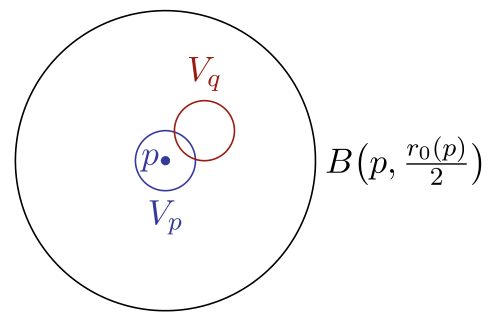
\includegraphics[width=0.48\textwidth]{figs/fig5_3_clean.png}
    \caption{流形坐标覆盖下邻域两两相交时的几何度量与支撑相容性.}
    \label{fig:5.3}
\end{figure}

\begin{proof}[定理~\ref{thm:5.32} 的证明]
由引理~\ref{lem:5.33}, 我们可以固定一个由满足 $\bar{U}_i$ 紧致的坐标卡 $F_i \colon U_i \to F_i(U_i) \subset \R^n$ 构成的开覆盖 $M = \bigcup_i U_i$, 使得只要 $U_i \cap U_j \neq \emptyset$, 并集 $U_i \cup U_j$ 就包含于某个坐标卡 $F_{ij} \colon U_{ij} \to F_{ij}(U_{ij}) \subset \R^n$ 之内.

假定 $A$ 是适正支集的. (若 $B$ 是适正支集的则论证完全对称.) 写出
\begin{equation}\label{eq:5.74}
    \begin{aligned}
        A &= K + \sum_i F_i^* A_i (F_i^{-1})^*, \qquad A_i \in \Psi_{\mathrm{c}}^m(F_i(U_i)), \quad K \in \mathcal{C}^\infty(M^2; \Omega_R), \\
        B &= K' + \sum_i F_i^* B_i (F_i^{-1})^*, \qquad B_i \in \Psi_{\mathrm{c}}^{m'}(F_i(U_i)), \quad K' \in \mathcal{C}^\infty(M^2; \Omega_R).
    \end{aligned}
\end{equation}
由于 $A$ 与所有的 $F_i^* A_i (F_i^{-1})^*$ 都是适正支集的, $K$ 亦为适正支集的. 逐项考察复合算子 $A \circ B$, 并追踪各分量 Schwartz 核的支集:

首先证明 $K \circ K' \in \Psi^{-\infty}(M)$. 我们有 $(K \circ K')(x, y) = \int_M K(x, z) K'(z, y)$. 对任意紧集 $K_1 \subset M$, 存在紧集 $K_2 \subset M$ (具体而言可取 $K_2 = \pi_R(\supp K \cap \pi_L^{-1}(K_1))$) 使得
\begin{equation}\label{eq:5.75}
    (K \circ K')(x, y) = \int_{K_2} K(x, z) K'(z, y), \qquad x \in K_1.
\end{equation}
因此 $K \circ K'$ 的 Schwartz 核属于 $\mathcal{C}^\infty(M^2; \Omega_R)$.

接着考察复合 $K_i \defeq K \circ F_i^* B_i (F_i^{-1})^*$. 它将 $u \in \mathscr{E}'(M)$ 映入 $\mathcal{C}^\infty(M)$; 且若 $\supp u \cap U_i = \emptyset$, 则 $K_i u = 0$. 于是由注记~\ref{rem:5.23},
\begin{equation}\label{eq:5.76}
    K_i \in \mathcal{C}^\infty(M^2; \Omega_R), \qquad \supp K_i \subset M \times U_i.
\end{equation}
类似地可证明
\begin{equation}\label{eq:5.77}
    K'_i \defeq F_i^* A_i (F_i^{-1})^* \circ K' \in \mathcal{C}^\infty(M^2; \Omega_R), \qquad \supp K'_i \subset U_i \times M.
\end{equation}
最后, 我们需要考察复合
\begin{equation}\label{eq:5.78}
    C_{ij} \defeq F_i^* A_i (F_i^{-1})^* \circ F_j^* B_j (F_j^{-1})^* \colon \SmoothComp(M) \to \mathcal{C}^\infty(M).
\end{equation}
当 $U_i \cap U_j = \emptyset$ 时, 该复合格外为 0. 当 $U_i \cap U_j \neq \emptyset$ 时, 由引理~\ref{lem:5.28}, 我们可将式~\eqref{eq:5.78} 等价写为
\begin{equation}\label{eq:5.79}
    F_{ij}^* A_{ij} (F_{ij}^{-1})^* \circ F_{ij}^* B_{ij} (F_{ij}^{-1})^* = F_{ij}^* (A_{ij} \circ B_{ij}) (F_{ij}^{-1})^*,
\end{equation}
其中 $A_{ij} \in \Psi_{\mathrm{c}}^m(F_{ij}(U_{ij}))$ 且 $B_{ij} \in \Psi_{\mathrm{c}}^{m'}(F_{ij}(U_{ij}))$. 由 $\R^n$ 上的复合定理 (定理~\ref{thm:4.22}), $A_{ij} \circ B_{ij} \in \Psi_{\mathrm{c}}^{m+m'}(F_{ij}(U_{ij}))$. 综上所述, $A \circ B \in \Psi^{m+m'}(M)$, 且当 $A, B$ 均是适正支集时其复合显然保持适正支集.
\end{proof}

\begin{corollary}[紧流形上的复合]\label{cor:5.34}
若 $M$ 为紧流形, 则 $\Psi^m(M) \circ \Psi^{m'}(M) \subset \Psi^{m+m'}(M)$.
\end{corollary}

\section{主符号}\label{sec:5.5}
\index{liuxingshang zhufuhao@流形上的主符号 (principal symbols on manifolds)}%

定理~\ref{thm:5.2} 中公式~\eqref{eq:5.2} 的精髓在于: 动量变量 $\xi$ 变换时所乘的逆转置矩阵 $(\kappa'(x)^T)^{-1}$, 恰恰是余切丛 $T^* M$ 在底流形坐标变换下余切向量的严格拉回变换法则! 这从根本上揭示出: 伪微分算子的主符号天生是定义在余切丛 $T^* M$ 上的几何对象.

\begin{definition}[向量丛上的符号空间]\label{def:5.35}
设 $\pi \colon E \to M$ 为秩为 $k$ 的光滑向量丛. 对 $m \in \R$, 符号空间 $S^m(E) \subset \mathcal{C}^\infty(E)$ 由所有满足如下条件的函数 $a \in \mathcal{C}^\infty(E)$ 组成: 在局部平凡化卡 $\tau \colon \pi^{-1}(U) \to F(U) \times \R^k$ 下,
\begin{equation}\label{eq:5.80}
    b(x, v) \defeq (\tau^{-1})^* (a|_{\pi^{-1}(U)})(x, v) \in \mathcal{C}^\infty(F(U) \times \R^k),
\end{equation}
且对任意 $\phi \in \SmoothComp(F(U))$, 均有 $\phi(x) b(x, v) \in S^m(\R^n; \R^k)$. 当 $E = T^* M$ 时, 我们得到余切丛上的符号空间 $S^m(T^* M)$.
\end{definition}

\begin{lemma}[坐标卡内定义的符号延拓]\label{lem:5.36}
在定义~\ref{def:5.35} 的记号下, 若 $\phi \in \SmoothComp(F(U))$, $b \in S^m(\R^n; \R^k)$, 则 $a \defeq \tau^*(\phi b) \in S^m(E)$.
\end{lemma}

\begin{proof}
在另一个坐标卡与平凡化下, 转变函数表达为
\begin{equation}\label{eq:5.81}
    b'(x, v) = \phi(\kappa(x)) b(\kappa(x), \Phi(x) v), \qquad x \in F'(U \cap U'),
\end{equation}
其中 $\kappa \defeq F \circ (F')^{-1} \colon F'(U \cap U') \to F(U \cap U')$, 且 $\Phi \colon F'(U \cap U') \to \mathrm{GL}(k, \R)$ 为光滑映射. 设 $\psi \in \SmoothComp(F'(U'))$, 则 $\chi(x) \defeq \psi(x) \phi(\kappa(x)) \in \SmoothComp(F'(U \cap U'))$. 我们需要验证
\begin{equation}\label{eq:5.82}
    \chi(x) b(\kappa(x), \Phi(x) v) \in S^m(\R^n; \R^k).
\end{equation}
这直接遵循式~\eqref{eq:5.14} 的完全同类求导计算.
\end{proof}

\begin{corollary}[通过坐标卡刻画符号空间]\label{cor:5.37}
设 $M = \bigcup_i U_i$ 为满足 $\bar{U}_i$ 紧致的局部有限坐标卡开覆盖, $\tau_i$ 为局部平凡化. 则 $a \in \mathcal{C}^\infty(E)$ 属于 $S^m(E)$ 当且仅当存在符号 $b_i \in S^m(\R^n; \R^k)$ 与 $\chi_i \in \SmoothComp(F_i(U_i))$ 使得
\begin{equation}\label{eq:5.83}
    a = \sum_i \tau_i^* (\chi_i b_i).
\end{equation}
\end{corollary}

现在, 给定算子 $A \in \Psi^m(M)$, 我们期望其主符号是商空间 $S^m(T^* M) / S^{m-1}(T^* M)$ 中的元素. 我们首先在局部进行定义: 设 $F \colon U \to F(U) \subset \R^n$ 为局部坐标卡且 $\bar{U}$ 紧致, 设开集 $V \subset U$ 满足 $\bar{V} \subset U$. 记 $\tau \colon T_U^* M \to F(U) \times \R^n$ 为由 $F$ 诱导的平凡化. 选取切断函数 $\chi \in \SmoothComp(U)$ 满足在 $\bar{V}$ 上 $\chi \equiv 1$. 则我们置
\begin{equation}\label{eq:5.84}
    a_V \defeq \left. \tau^*\left( \sigma_L((F^{-1})^* \chi A \chi F^*) \right) \right|_{T_V^* M} \in S^m(T_V^* M).
\end{equation}
由欧氏空间上的局部理论 (特别是定理~\ref{thm:5.2}), 等价类
\begin{equation}\label{eq:5.85}
    [a_V] \in S^m(T_V^* M) / S^{m-1}(T_V^* M)
\end{equation}
与 $\chi$ 的选取以及覆盖 $\bar{V}$ 邻域的坐标系 $F$ 的选取均无关. 此外, 若 $V' \subset V$, 则限制到 $V'$ 满足 $[a_V]|_{V'} = [a_{V'}]$.

\begin{definition}[流形上伪微分算子的主符号]\label{def:5.38}
算子 $A \in \Psi^m(M)$ 的\textbf{主符号}是唯一满足如下性质的元素
\begin{equation}\label{eq:5.86}
    \sigma_m(A) \in S^m(T^* M) / S^{m-1}(T^* M):
\end{equation}
若 $a \in S^m(T^* M)$ 为 $\sigma_m(A)$ 的任意代表元且 $V$ 如上, 则 $[a|_{T_V^* M}] = [a_V] \in S^m(T_V^* M) / S^{m-1}(T_V^* M)$.
\end{definition}

该定义蕴含了主符号 $\sigma_m(A)$ 存在且唯一的断言. 存在性由 $[a_V]$ 的相容性质直接得出: 选取开覆盖 $\{V\}$ 的局部有限子覆盖 $\{V_i\}$ 及其从属单位分解 $\{\phi_i\}$, 由推论~\ref{cor:5.37} $a \defeq \sum_i \phi_i a_{V_i} \in S^m(T^* M)$; 我们随后令
\begin{equation}\label{eq:5.87}
    \sigma_m(A) \defeq [a].
\end{equation}
对任意开集 $V$ 及 $\phi \in \SmoothComp(V)$, 在 $V$ 上有
\begin{equation}\label{eq:5.88}
    \phi a = \sum_i \tilde{\phi}_i (\phi_i \phi a_{V_i}) = \sum_i \tilde{\phi}_i (\phi_i \phi a_V + e_i) = \phi a_V + \sum_i \tilde{\phi}_i e_i,
\end{equation}
其中 $\sum_i \tilde{\phi}_i e_i \in S^{m-1}(T^* M)$. 唯一性同理得出.

\begin{proposition}[流形上主符号短正合列]\label{prop:5.39}
主符号映射给出如下短正合列:
\begin{equation}\label{eq:5.89}
    0 \to \Psi^{m-1}(M) \hookrightarrow \Psi^m(M) \xrightarrow{\sigma_m} S^m(T^* M) / S^{m-1}(T^* M) \to 0.
\end{equation}
\end{proposition}

\begin{proof}
我们只需证明 $\sigma_m$ 的满射性. 选取从属于坐标卡开覆盖 $M = \bigcup_i U_i$ ($\bar{U}_i$ 紧致, 坐标映射为 $F_i \colon U_i \to F_i(U_i) \subset \R^n$) 的局部有限单位分解 $\{\phi_i\}$. 将任意给定的 $a \in S^m(T^* M)$ 分解为 $a = \sum_i \phi_i a$. 只需证明存在 Schwartz 核支集包含于 $U_i \times U_i$ 之内的算子 $A_i \in \Psi^m(M)$ 满足 $\sigma_m(A_i) = [\phi_i a]$, 随后即可取局部有限和 $A = \sum_i A_i$. 这很容易做到: 若取 $\tilde{\phi}_i \in \SmoothComp(U_i)$ 满足在 $\supp\phi_i$ 上 $\tilde{\phi}_i \equiv 1$, 则算子
\begin{equation}\label{eq:5.90}
    A_i = F_i^* \Op\left( \left( (F_i^{-1})^* \phi_i \right)(x) a(x, \xi) \left( (F_i^{-1})^* \tilde{\phi}_i \right)(y) \right) (F_i^{-1})^*
\end{equation}
即满足所求条件.
\end{proof}

由欧氏空间上的相应结论 (命题~\ref{prop:4.24}) 立即推出:

\begin{proposition}[主符号的乘法性]\label{prop:5.40}
若 $A \in \Psi^m(M)$, $B \in \Psi^{m'}(M)$, 且其中至少有一个是适正支集的, 则
\begin{equation}\label{eq:5.91}
    \sigma_{m+m'}(A \circ B) = \sigma_m(A) \sigma_{m'}(B).
\end{equation}
\end{proposition}

关于换位子主符号的对等结论 (命题~\ref{prop:4.25}) 将在第~\ref{sec:5.14}~节中讨论.

\section{量化}\label{sec:5.6}
\index{lianghua@量化 (quantization)}%

一般而言, 并不存在一种完全自然的方式将 $T^* M$ 上的符号量化为 $M$ 上的伪微分算子. 然而, 我们有如下极为实用的构造: 固定坐标卡覆盖 $M = \bigcup_i U_i$ (满足 $\bar{U}_i$ 紧致, $F_i \colon U_i \to F_i(U_i) \subset \R^n$) 构成的局部有限开覆盖, 并设 $\{\phi_i\} \subset \SmoothComp(U_i)$ 为从属于 $\{U_i\}$ 的单位分解. 固定 $\tilde{\phi}_i \in \SmoothComp(U_i)$ 使得在 $\supp\phi_i$ 附近 $\tilde{\phi}_i \equiv 1$. 给定 $a \in S^m(T^* M)$, 定义
\begin{equation}\label{eq:5.92}
    \Op(a) \defeq \sum_i F_i^* \Op\left( \left( (F_i^{-1})^* \phi_i \right)(x) \left( (\tau_i^{-1})^* a \right)(x, \xi) \left( (F_i^{-1})^* \tilde{\phi}_i \right)(y) \right) (F_i^{-1})^*,
\end{equation}
其中 $\tau_i \colon T^*_{U_i} M \to F_i(U_i) \times \R^n$ 为由 $F_i$ 诱导的平凡化. 由定理~\ref{thm:5.29}, 式~\eqref{eq:5.92} 定义了映射
\begin{equation}\label{eq:5.93}
    \Op \colon S^m(T^* M) \to \Psi^m(M).
\end{equation}

\begin{proposition}[量化映射的性质]\label{prop:5.41}
式~\eqref{eq:5.93} 中的映射 $\Op$ 是连续线性的, 且取值于适正支集算子组成的子空间中. 我们有 $\Op(1) = I$ (恒等算子). 此外, $\Op \colon S^m(T^* M) \to \Psi^m(M)$ 模去 $\Psi^{-\infty}(M)$ 是满射; 即 $\Psi^m(M) = \Op(S^m(T^* M)) + \Psi^{-\infty}(M)$.
\end{proposition}

\begin{proof}
我们仅给出最后一个断言的证明概要. 在式~\eqref{eq:5.66} 的记号下, 我们可以将任意给定的 $A \in \Psi^m(M)$ 写为 $A \defeq A_m + K$ 的形式, 其中 $A_m = \sum_i F_i^* B_i (F_i^{-1})^*$, 且 $K \in \Psi^{-\infty}(M)$. 我们将算子 $B_i \in \Psi_{\mathrm{c}}^m(F_i(U_i))$ 的符号沿着平凡化 $\tau_i$ 的拉回求和, 得到符号 $a_m \in S^m(T^* M)$; 由主符号的坐标不变性可知,
\begin{equation}\label{eq:5.94}
    A_{m-1} \defeq A_m - \Op(a_m) \in \Psi^{m-1}(M).
\end{equation}
随后我们可将定理~\ref{thm:5.29} 应用于 $A_{m-1}$. 归纳论证由此产生 $a_{m-j} \in S^{m-j}(T^* M)$ ($j \in \N$), 使得 $A_{m-j-1} \defeq A_{m-j} - \Op(a_{m-j}) \in \Psi^{m-j-1}(M)$. 取 $a \in S^m(T^* M)$ 为 $a_{m-j}$ ($j \in \N_0$) 的渐近和, 我们最终得到
\begin{equation}\label{eq:5.95}
    A = A_m + K = \Op(a) + K + R, \qquad R \in \Psi^{-\infty}(M).
\end{equation}
其中 $K + R$ 是光滑的残余算子.
\end{proof}

\section{作用在向量丛截面上的算子}\label{sec:5.7}
\index{xiangliangcong@向量丛截面算子 (operators on sections)}%

读者可能会问, 为什么我们迄今为止尚未讨论 $A \in \Psi^m(M)$ (甚至 $A \in \Diff^m(M)$) 的伴随算子. 由于我们并没有一种在流形 $M$ 上积分函数的内在不变方式, 定义 $A^*$ 唯一合理的方式是通过
\begin{equation}\label{eq:5.96}
    \int_M (A u)(x) \overline{v(x)} = \int_M u(x) \overline{A^* v(x)}, \qquad u \in \SmoothComp(M), \quad v \in \SmoothComp(M; \Omega M);
\end{equation}
换言之, $A^*$ 应当是一个作用在 $1$-密度上的算子. 我们将把将 $E$ 的截面映为 $F$ 的截面的 $m$ 阶微分算子空间 $\Diff^m(M; E, F)$ 的定义留给读者作为练习, 直接进入伪微分算子的情形.

\begin{definition}[作用在向量丛截面上的伪微分算子]\label{def:5.42}
设 $M$ 为光滑流形, $\pi_E \colon E \to M$ 与 $\pi_F \colon F \to M$ 为秩分别为 $k_E, k_F$ 的两个实向量丛 (复向量丛的情形完全对等). 则 $\Psi^m(M; E, F)$ 是所有满足如下性质的线性算子
\begin{equation}\label{eq:5.97}
    A \colon \SmoothComp(M; E) \to \Smooth(M; F)
\end{equation}
构成的空间:
\begin{enumerate}
    \item 设 $U \subset M$ 为任意开集, $G \colon U \to G(U) \subset \R^n$ 为微分同胚, 且设 $\tau_E \colon \pi_E^{-1}(U) \to G(U) \times \R^{k_E}$, $\tau_F \colon \pi_F^{-1}(U) \to G(U) \times \R^{k_F}$ 为 $E, F$ 的局部平凡化. 利用 $\tau_E$, 将 $E$ 在 $U$ 上的光滑截面等同于 $U$ 上的光滑函数 $k_E$-元组, 对 $F$ 的截面亦然. 若 $\psi \in \SmoothComp(U)$, 则存在一个伪微分算子的 $k_F \times k_E$ 矩阵 $B = (B_{ij})$, 其中 $B_{ij} \in \Psi_{\mathrm{c}}^m(G(U))$, 使得在 $U$ 上有
    \begin{equation}\label{eq:5.98}
        (\psi A(\psi u))_i = \sum_{j=1}^{k_E} G^* \left( B_{ij} ((G^{-1})^* u)_j \right), \qquad u \in \SmoothComp(M; E), \quad i = 1, \ldots, k_F.
    \end{equation}
    \item 若 $\phi, \psi \in \Smooth(M)$ 满足 $\supp\phi \cap \supp\psi = \emptyset$, 则存在光滑核 $K \in \Smooth(M^2; \pi_L^* F \otimes \pi_R^*(E^* \otimes \Omega M))$ 使得 $\phi A \psi = K$.
\end{enumerate}
在 $F = E$ 的特例下, 我们记 $\Psi^m(M; E) \defeq \Psi^m(M; E, E)$.
\end{definition}

在局部坐标与平凡化下, 算子 $A \in \Psi^m(M; E, F)$ 的符号是以 $\R^{k_E} \to \R^{k_F}$ 的线性映射为取值的符号. 其内在不变定义如下: 记 $\pi \colon T^* M \to M$ 为投影. 给定向量丛 $G \to M$, 我们可以考虑其拉回丛 $\pi^* G \to T^* M$ (定义~\ref{def:5.9}); $G$ 在开集 $U \subset M$ 上的平凡化 $G|_U \cong U \times \R^{k_G}$, 在 $T^*_U M$ 上诱导了在 ``$T^* M$ 纤维上常值'' 的拉回丛平凡化:
\begin{equation}\label{eq:5.99}
    (\pi^* G)|_{T^*_U M} \cong T^* U \times \R^{k_G},
\end{equation}
即通过局部平凡化等同 $(\pi^* G)_{(x, \xi)} = G_x \cong \R^{k_G}$. 我们随后用
\begin{equation}\label{eq:5.100}
    S^m(T^* M; \pi^* G) \subset \Smooth(T^* M; \pi^* G)
\end{equation}
表示所有在局部坐标以及 $G$ 的平凡化下 (该平凡化如式~\eqref{eq:5.99} 般诱导了 $\pi^* G$ 的平凡化) 呈现为 $\R^n$ 上 $m$ 阶符号的 $k_G$-向量的光滑截面空间. 内在地,
\begin{equation}\label{eq:5.101}
    \sigma_m(A) \in (S^m / S^{m-1})(T^* M; \pi^* \mathrm{Hom}(E, F)).
\end{equation}
这意味着 $\sigma_m(A)$ 的一个代表元是一个将每个 $(x, \xi) \in T^* M$ 映为 $\mathrm{Hom}(E_x, F_x)$ 中元素的映射. 我们有短正合列:
\begin{equation}\label{eq:5.102}
    0 \to \Psi^{m-1}(M; E, F) \hookrightarrow \Psi^m(M; E, F) \xrightarrow{\sigma_m} (S^m / S^{m-1})(T^* M; \pi^* \mathrm{Hom}(E, F)) \to 0.
\end{equation}

第~\ref{sec:5.4}--\ref{sec:5.5}~节中的结论完全延拓至此; 此外, 我们还可以定义伴随算子:

\begin{proposition}[复合与伴随]\label{prop:5.43}
设 $M$ 为光滑流形, $E, F, G \to M$ 为三个向量丛.
\begin{enumerate}
    \item 设 $A \in \Psi^m(M; F, G)$, $B \in \Psi^{m'}(M; E, F)$, 且其中至少有一个是适正支集的. 则 $A \circ B \in \Psi^{m+m'}(M; E, G)$, 且 $\sigma_{m+m'}(A \circ B) = \sigma_m(A) \circ \sigma_{m'}(B)$.
    \item 设 $A \in \Psi^m(M; E, F)$. 则其 (实) 伴随算子 $A^T$ 通过
    \begin{equation}\label{eq:5.103}
        \int_M (A u) v = \int_M u (A^T v), \qquad u \in \SmoothComp(M; E), \quad v \in \SmoothComp(M; F^* \otimes \Omega M)
    \end{equation}
    定义, 是一个伪微分算子:
    \begin{equation}\label{eq:5.104}
        A^T \in \Psi^m(M; F^* \otimes \Omega M, E^* \otimes \Omega M),
    \end{equation}
    且满足 $\sigma_m(A^T) = \sigma_m(A)^T$. 若 $A$ 为适正支集的, 则 $A^T$ 亦为适正支集的.
\end{enumerate}
\end{proposition}

\begin{remark}[具备额外结构的向量丛]\label{rem:5.44}
\begin{enumerate}
    \item 若 $E, F$ 为带有反线性对合 (``复共轭'') 的复向量丛, 则可以类似于式~\eqref{eq:5.103} 定义伴随算子 $A^*$, 但在第二个因子上取复共轭; 此时有
    \begin{equation}\label{eq:5.105}
        A^* \in \Psi^m(M; F^* \otimes \Omega M, E^* \otimes \Omega M), \qquad \sigma_m(A^*) = \sigma_m(A)^*.
    \end{equation}
    这特别适用于 $E = F = M \times \mathbb{C}$ 的情形, 此时 $E, F$ 的截面即为 $M$ 上的复数值函数.
    \item $E$ 上的内积诱导了同构 $E^* \cong E$ (当内积为半双线性时该同构为反线性的). 若进一步选取 $\Omega M$ 的一个平凡化, 则 $A^T \in \Psi^m(M; F, E)$ (在复情形下 $A^* \in \Psi^m(M; E, F)$).
\end{enumerate}
\end{remark}

式~\eqref{eq:5.104} 的一个直接推论是如下命题~\ref{prop:5.27} 的推广:

\begin{corollary}[伪微分算子在分布与光滑截面上的作用]\label{cor:5.45}
设 $A \in \Psi^m(M; E, F)$. 则 $A$ 延拓为有界线性算子 $A \colon \mathcal{E}'(M; E) \to \mathcal{D}'(M; F)$. 若 $A$ 是适正支集的, 则 $A$ 还将 $\mathcal{D}'(M; E) \to \mathcal{D}'(M; F)$, 且经限制给出映射 $\Smooth(M; E) \to \Smooth(M; F)$.
\end{corollary}

\begin{proof}
$A^T$ 是有界映射 $\SmoothComp(M; F^* \otimes \Omega M) \to \Smooth(M; E^* \otimes \Omega M)$. 因此我们可以利用式~\eqref{eq:5.104} 通过对偶性定义 $A \colon \mathcal{E}'(M; E) \to \mathcal{D}'(M; F)$; 当限制在 $\SmoothComp(M; E)$ 上时, 它与原算子 $A$ 完全吻合.

若 $A$ 是适正支集的, 则 $A^T$ 将 $\SmoothComp(M; F^* \otimes \Omega M) \to \SmoothComp(M; E^* \otimes \Omega M)$, 从而我们现在可以通过对偶性定义 $A \colon \mathcal{D}'(M; E) \to \mathcal{D}'(M; F)$. 最后注意到 $\Smooth(M; E) \subset \mathcal{D}'(M; E)$; 故只需检验当 $u \in \Smooth(M; E)$ 时 $A u \in \Smooth(M; F)$. 利用紧支单位分解 $1 = \sum_i \phi_i$, 我们有
\begin{equation}\label{eq:5.106}
    A u = A\left( \sum_i \phi_i u \right) = \sum_i A(\phi_i u),
\end{equation}
该式在 $\mathcal{D}'(M; F)$ 中收敛. 由于 $A$ 是适正支集的, 最后的求和是光滑项的局部有限和, 因而其和是光滑截面.
\end{proof}

\section{算子的特殊类别}\label{sec:5.8}
\index{jingdian weifen suanzi@经典伪微分算子 (classical ps.d.o.)}%

设 $M$ 为流形, $E, F \to M$ 为秩为 $k_E, k_F$ 的向量丛.

\begin{definition}[流形上的经典伪微分算子]\label{def:5.46}
设 $m \in \R$. 经典伪微分算子子空间 $\Psi_{\mathrm{cl}}^m(M; E, F) \subset \Psi^m(M; E, F)$ 由所有满足如下条件的算子组成: 其在局部坐标卡以及 $E, F$ 的局部平凡化下的全符号, 是由 $m$ 阶经典符号构成的 $k_F \times k_E$ 矩阵. $\Psi_{\mathrm{cl}}^m(M; E, F)$ 上的主符号映射记录其最高阶齐次部分:
\begin{equation}\label{eq:5.107}
    \sigma_m \colon \Psi_{\mathrm{cl}}^m(M; E, F) \to S_{\mathrm{hom}}^m(T^* M \setminus o; \pi^* \mathrm{Hom}(E, F)).
\end{equation}
\end{definition}

这是一个合理的定义, 因为经典性在局部坐标变换下保持不变; 这直接遵循定理~\ref{thm:5.2} 的证明, 尤其是式~\eqref{eq:5.13}. 读者容易验证两个经典伪微分算子的复合 (其中至少一个是适正支集的) 依然是经典伪微分算子, 且取伴随运算同样保持经典性. 我们有
\begin{equation}\label{eq:5.108}
    \Diff^m(M; E, F) \subset \Psi_{\mathrm{cl}}^m(M; E, F).
\end{equation}

作用在向量丛截面上的算子中一个重要特殊类别如下 (参见例~\ref{eg:5.55}):

\begin{definition}[主标量算子]\label{def:5.47}
设 $m \in \R$ 且 $A \in \Psi^m(M; E)$. 若 $A$ 的主符号在 $E$ 的纤维上是标量乘法, 即存在符号 $a \in S^m(T^* M)$ 使得 $\sigma_m(A)(x, \xi) = a(x, \xi) \mathrm{Id}_{E_x}$, 则称 $A$ 是\textbf{主标量的} (principally scalar).
\end{definition}

\section{紧流形上的椭圆算子与 Fredholm 理论}\label{sec:5.9}
\index{tuoyuan suanzi@椭圆算子 (elliptic operator)}%
\index{Fredholm suanzi@Fredholm 算子 (Fredholm operator)}%
\index{guangyini@广义逆 (generalized inverse)}%

设 $M$ 为无边界 $n$ 维流形, $E, F \to M$ 为两个向量丛.

\begin{definition}[椭圆性]\label{def:5.48}\sloppy
设 $A \in \Psi^m(M; E, F)$, 其主符号记为 $a = \sigma_m(A)$. 若存在符号 $b \in S^{-m}(T^* M; \pi^* \mathrm{Hom}(F, E))$ 使得
\[
    a b - 1 \in S^{-1}(T^* M; \pi^* \mathrm{End}(F)), \qquad b a - 1 \in S^{-1}(T^* M; \pi^* \mathrm{End}(E)),
\]
则称 $A$ 是\textbf{椭圆型的} (elliptic).
\end{definition}

\begin{remark}[椭圆性的等价定义]\label{rem:5.49}
由式~\eqref{eq:4.105} 中的抽象群论论证, 如下定义与 $A$ 的椭圆性等价: 存在符号 $b, b' \in S^{-m}(T^* M; \pi^* \mathrm{Hom}(F, E))$ 使得 $a b - 1 \in S^{-1}(T^* M; \pi^* \mathrm{End}(F))$ 以及 $b' a - 1 \in S^{-1}(T^* M; \pi^* \mathrm{End}(E))$.
\end{remark}

椭圆拟逆构造 (定理~\ref{thm:4.29}) 在此框架下同样成立; 证明留给读者.

\begin{theorem}[椭圆拟逆]\label{thm:5.50}
设 $A \in \Psi^m(M; E, F)$ 是椭圆型的. 则存在适正支集算子 $B \in \Psi^{-m}(M; F, E)$, 在模去 $\Psi^{-\infty}(M; F, E)$ 的意义下唯一, 使得 $A \circ B - I \in \Psi^{-\infty}(M; F)$, $B \circ A - I \in \Psi^{-\infty}(M; E)$. 若 $A$ 是经典的, 则 $B$ 亦为经典的.
\end{theorem}

例~\ref{eg:5.26} 提供了紧流形上椭圆微分算子可逆的一个例子. 不可逆算子具有拟逆的典型例子如下:

\begin{example}[圆周上的导数算子]\label{eg:5.51}
设 $M = \mathbb{S}^1 \defeq \R_\theta / 2\pi\mathbb{Z}$, 并设 $A = D_\theta \in \Psi^1(M)$. 该算子在任何包含非零常数函数的函数空间上均不可逆. $D_\theta$ 在 $\R_\theta$ 上的一个基本解由 $\ii H(\theta)$ 给出. 通过在 $\theta = 0$ 之外进行切断, 可以在 $\mathbb{S}^1$ 上为 $A$ 构造一个拟逆 $B$. 具体而言, 若 $\chi \in \SmoothComp((-\pi, \pi))$ 在 $0$ 附近等于 1, 则我们可以取 $B$ 具有 Schwartz 核
\begin{equation}\label{eq:5.109}
    K_B(\theta, \theta') \defeq -\frac{1}{2} |\theta - \theta'| \chi(\theta - \theta') |\dd\theta'|, \qquad \theta, \theta' \in (-\pi, \pi),
\end{equation}
这是 $\mathcal{D}'(M^2; \Omega_R)$ 的一个元素. 读者可验证这确立了 $B \in \Psi_{\mathrm{cl}}^{-1}(M)$.
\end{example}

\begin{theorem}[紧流形上椭圆伪微分算子的 Fredholm 性质与广义逆]\label{thm:5.52}
设 $M$ 为紧流形, $A \in \Psi^m(M; E, F)$ 为椭圆型算子.
\begin{enumerate}
    \item 算子 $A \colon \Smooth(M; E) \to \Smooth(M; F)$ 是 Fredholm 算子, 即 $\ker A$ 为有限维空间, 且 $\ran A$ 是闭子空间并具有有限余维数. 进一步地,
    \begin{equation}\label{eq:5.110}
        \ran A = \left\{ f \in \Smooth(M; F) : \langle f^*, f \rangle = 0, \; \forall f^* \in \Smooth(M; F^* \otimes \Omega M) \text{ 满足 } A^T f^* = 0 \right\},
    \end{equation}
    其中 $A^T \in \Psi^m(M; F^* \otimes \Omega M, E^* \otimes \Omega M)$.
    \item 设 $0 < \nu \in \Smooth(M; \Omega M)$ 为 $M$ 上的体积密度, 并在 $E, F$ 上固定正定纤维内积. 线性算子 $G \colon \Smooth(M; F) \to \Smooth(M; E)$ 由如下条件唯一确定:
    \begin{equation}\label{eq:5.111}
        \begin{aligned}
            G f &= u, \quad \text{若 } f \in \ran A, \; A u = f, \; u \perp \ker A \text{ 于 } L^2(M; E; \nu) \text{ 中}, \\
            G f &= 0, \quad \text{若 } f \perp \ran A \text{ 于 } L^2(M; F; \nu) \text{ 中}.
        \end{aligned}
    \end{equation}
    该算子称为 $A$ 的\textbf{广义逆} (generalized inverse). 它满足 $G \in \Psi^{-m}(M; F, E)$ 以及
    \begin{equation}\label{eq:5.112}
        G A = I - \pi_N, \qquad A G = I - \pi_R,
    \end{equation}
    其中 $\pi_N \colon L^2(M; E; \nu) \to L^2(M; E; \nu)$ 为到 $\ker A$ 上的正交投影, $\pi_R \colon L^2(M; F; \nu) \to L^2(M; F; \nu)$ 为到 $\ker A^* = (\ran A)^\perp$ 上的正交投影. 我们有 $\pi_N \in \Psi^{-\infty}(M; E)$ 以及 $\pi_R \in \Psi^{-\infty}(M; F)$. 特别地, 若 $A$ 可逆, 则 $G = A^{-1} \in \Psi^{-m}(M; F, E)$.
\end{enumerate}
\end{theorem}

\begin{proof}
我们在 $M$ 上固定体积密度, 并在 $E, F$ 上固定正定纤维内积. 设 $B \in \Psi^{-m}(M; F, E)$ 为 $A$ 的椭圆拟逆, 故
\begin{equation}\label{eq:5.113}
    R_1 \defeq A B - I \in \Psi^{-\infty}(M; F), \qquad R_2 \defeq B A - I \in \Psi^{-\infty}(M; E).
\end{equation}
我们首先证明 $\dim\ker A < \infty$. 注意到
\begin{equation}\label{eq:5.114}
    u \in \mathcal{D}'(M; E), \quad A u = 0 \implies u = (B A - R_2) u = -R_2 u \in \Smooth(M; E).
\end{equation}
从这一角度来看, 恒等映射在 $\ker A \subset L^2(M; E; \nu)$ 上可表为 $I = B A - R_2 = -R_2$. 现在, $R_2$ 将 $L^2(M; E; \nu) \to \Smooth(M; E)$, 从而由 Arzelà--Ascoli 定理可知, 作为 $L^2(M; E; \nu) \to L^2(M; E; \nu)$ 的映射, $R_2$ 是紧算子. 因此, 闭子空间 $\ker A \subset L^2(M; E; \nu)$ 中的单位球是紧集; 从而 $\ker A \subset L^2(M; E; \nu)$ 是有限维的.

接下来我们证明 $\ran A$ 是闭的. 设 $f_j = A u_j \to f \in \Smooth(M; F)$, 其中 $u_j \in \Smooth(M; E)$. 我们可以对 $u_j$ 加上 $\ker A$ 中的元素, 从而不妨假设 $u_j \perp \ker A$. 我们有
\begin{equation}\label{eq:5.115}
    u_j = B A u_j - R_2 u_j = B f_j - R_2 u_j.
\end{equation}
假定在某个子列上 $\|u_j\|_{L^2} \to \infty$. 则
\begin{equation}\label{eq:5.116}
    \frac{u_j}{\|u_j\|_{L^2}} = B\left( \frac{f_j}{\|u_j\|_{L^2}} \right) - R_2\left( \frac{u_j}{\|u_j\|_{L^2}} \right).
\end{equation}
该序列在 $\Smooth(M; E)$ 中有界, 从而我们可以提取在 $L^2(M; E; \nu)$ 中收敛的子列, 记为 $u_j / \|u_j\|_{L^2} \to u \in L^2(M; E; \nu)$. 于是 $A u = \lim_{j\to\infty} f_j / \|u_j\|_{L^2} = 0$, 故 $u \in \ker A$, 但由构造亦有 $u \perp \ker A$. 由于 $\|u\|_{L^2} = 1$, 这产生矛盾.

因此, $\|u_j\|_{L^2}$ 必定是有界的. 式~\eqref{eq:5.115} 随即表明 $u_j$ 在 $\Smooth(M; E)$ 中有界, 因而具有在 $\Smooth(M; E)$ 中收敛到 $u \in \Smooth(M; E)$ 的子列. 将 $u_j$ 替换为此子列, 我们得到
\begin{equation}\label{eq:5.117}
    A u = \lim_{j\to\infty} A u_j = \lim_{j\to\infty} f_j = f.
\end{equation}
这证明了值域 $\ran A$ 的闭性.

由于 $A^*$ 是椭圆型的, $\ran A$ 的有限余维数是式~\eqref{eq:5.110} 的直接推论. 式~\eqref{eq:5.110} 本身遵循如下两个事实:
\begin{enumerate}
    \item[(i)] 由于 $R = \ran A \subset \Smooth(M; F)$ 是 Fréchet 空间的闭子空间, 我们有 $R = {}^\perp(R^\perp) \defeq \{f \in \Smooth(M; F) : \langle f^*, f \rangle = 0, \; \forall f^* \in R^\perp\}$, 其中
        \begin{equation}\label{eq:5.118}
            R^\perp = \left\{ f^* \in \Distr(M; F^* \otimes \Omega M) : \langle f^*, f \rangle = 0, \; \forall f \in R \right\}
        \end{equation}
        是 $R$ 的零化子. 事实上, 包含关系 $R \subset {}^\perp(R^\perp)$ 显然成立. 为证反向包含, 设 $f_0 \in \Smooth(M; F) \setminus R$. Hahn--Banach 定理(利用 $R$ 的闭性) 给出一个连续线性泛函 $f^* \colon \Smooth(M; F) \to \mathbb{C}$, 即 $f^* \in \Distr(M; F^* \otimes \Omega M)$, 它在 $R$ 上为零 (从而 $f^* \in R^\perp$) 但 $\langle f^*, f_0 \rangle = 1$, 故 $f_0 \notin {}^\perp(R^\perp)$.
    \item[(ii)] 我们有 $f^* \in R^\perp$ 当且仅当对所有 $u \in \Smooth(M; E)$ 均有 $0 = \langle f^*, A u \rangle = \langle A^* f^*, u \rangle$, 即当且仅当 $f^* \in \ker A^*$.
\end{enumerate}
由于 $A^*$ 是椭圆型的, 故 $\ker A^* \subset \Smooth(M; F^* \otimes \Omega M)$, 式~\eqref{eq:5.110} 由此确立.

固定 $\ker A$ 的一组标准正交基 $\{u_1, \ldots, u_J\} \subset \Smooth(M; E)$, 到 $\ker A$ 上的正交投影 $\pi_N$ 表为
\begin{equation}\label{eq:5.119}
    \pi_N = \sum_{j=1}^J u_j \langle \cdot, u_j \rangle_{L^2(M; E; \nu)}.
\end{equation}
因此, 它具有光滑的 Schwartz 核. 类似论证表明到 $(\ran A)^\perp = \ker A^* \subset \Smooth(M; F)$ 上的正交投影 $\pi_R \colon L^2(M; F; \nu) \to L^2(M; F; \nu)$ 同样具有光滑 Schwartz 核. 从而 $\pi_N, \pi_R \in \Psi^{-\infty}$.

广义逆式~\eqref{eq:5.111} 属于 $\Psi^{-m}(M; F, E)$ 的断言现在通过如下恒等式推出:
\begin{equation}\label{eq:5.120}
    \begin{aligned}
        G &= G(A B - R_1) = (I - \pi_N) B - G R_1 \\
        &= (I - \pi_N) B - (B A - R_2) G R_1 \\
        &= (I - \pi_N) B - B(I - \pi_R) R_1 + R_2 G R_1.
    \end{aligned}
\end{equation}
事实上, 第一项属于 $\Psi^{-m}(M; F, E)$, 第二项属于 $\Psi^{-\infty}(M; F, E)$, 而最后一项是平滑算子, 从而亦属于 $\Psi^{-\infty}(M; F, E)$.
\end{proof}

作为一个典型范例, 我们讨论紧致 $n$ 维流形 $M$ 上的 Laplace 算子 (为简便计假设 $M$ 是连通的). 记 $S^2 T^* M$ 为 $T^* M$ 的二次对称张量幂. 设 $g \in \Smooth(M; S^2 T^* M)$ 为 Riemann 度量, 在局部坐标下表示为
\begin{equation}\label{eq:5.121}
    g = \sum_{i,j=1}^n g_{ij}(x) \frac{1}{2}(\dd x^i \otimes \dd x^j + \dd x^j \otimes \dd x^i), \qquad g_{ij}(x) = g_{ji}(x),
\end{equation}
其中 $(g_{ij}(x))_{i,j=1,\ldots,n}$ 正定. 记 $g^{ij}(x) = (g^{-1}(x))_{ij}$ 以及 $|g| = |\!\det(g_{ij})|$. 则 (标量) Laplace 算子为
\begin{equation}\label{eq:5.122}
    \Delta_g u \defeq \sum_{i,j=1}^n |g|^{-1/2} D_{x_i} \left( |g|^{1/2} g^{ij} D_{x_j} u \right).
\end{equation}
它满足
\begin{equation}\label{eq:5.123}
    \Delta_g \in \Diff^2(M), \qquad \sigma_2(\Delta_g)(x, \xi) = \sum_{i,j=1}^n g^{ij}(x) \xi_i \xi_j = |\xi|_{g_x^{-1}}^2.
\end{equation}
从而 $\Delta_g$ 是椭圆型的. 由定理~\ref{thm:5.52}, $\Delta_g$ 的核与余核均为有限维空间.

此外, 关于 $L^2(M; |\dd g|)$ 上的内积, $\Delta_g$ 是对称算子, 其中 $|\dd g| \in \Smooth(M; \Omega M)$ 是度量体积密度, 在局部坐标下由
\begin{equation}\label{eq:5.124}
    |\dd g| = |g(x)|^{1/2} |\dd x|
\end{equation}
定义. 从而 $\ker\Delta_g = (\ran\Delta_g)^\perp$; 且若 $u \in \ker\Delta_g$, 则
\begin{equation}\label{eq:5.125}
    0 = \int_M (\Delta_g u) \bar{u} \,|\dd g| = \int_M |\nabla u|_g^2 \,|\dd g|,
\end{equation}
其中 $|\nabla u|_g^2 \defeq \sum_{i,j=1}^n g^{ij}(\partial_{x_i} u)(\partial_{x_j} \bar{u})$, 故 $u$ 必为常数. 在定理~\ref{thm:5.52} 的记号下, 投影算子
\begin{equation}\label{eq:5.126}
    \pi_N = \frac{1}{\mathrm{vol}(M)} \langle \cdot, 1 \rangle 1 = \pi_R
\end{equation}
均等于到常数函数空间上的正交投影.

我们现在研究方程
\begin{equation}\label{eq:5.127}
    \Delta_g u = f, \qquad f \in \mathcal{D}'(M).
\end{equation}
设 $G \in \Psi^{-2}(M)$ 为 $\Delta_g$ 的广义逆. 在定理~\ref{thm:5.52} 的记号下,
\begin{equation}\label{eq:5.128}
    u = (G \Delta_g + \pi_N) u = G f + \pi_N u.
\end{equation}
这给出式~\eqref{eq:5.127} 的解当且仅当 $f = \Delta_g u = \Delta_g G f + \Delta_g \pi_N u = (I - \pi_R) f$. 由此得到:

\begin{proposition}[紧流形上的 Laplace 方程]\label{prop:5.53}
方程~\eqref{eq:5.127} 存在解 $u \in \mathcal{D}'(M)$ 当且仅当 $\langle f, 1 \rangle = 0$, 并且此时 $u$ 在相差一个加性常数意义下唯一. 若 $f \in \Smooth(M)$, 则 $u \in \Smooth(M)$. 若 $f \in \mathcal{D}'(M)$ 且 $p \notin \singsupp f$, 则存在 $p$ 的开邻域 $U \subset M$ 使得在 $U$ 上 $u \in \Smooth(U)$.
\end{proposition}

\begin{proof}
除最后一句话外, 其余结论由上述讨论直接保证. 最后一句话由广义逆 $G \in \Psi^{-2}(M)$ 的拟局部性推出: 选取 $\phi \in \SmoothComp(U)$ 在 $p$ 附近恒等于 1 且满足 $\supp\phi \cap \singsupp f = \emptyset$. 则 $\phi u = \phi G(\phi f) + \phi G((1-\phi)f) + c\phi$. 由于 $\phi f \in \SmoothComp(U)$, 故 $\phi G(\phi f) \in \Smooth$. 由于 $\phi$ 与 $1-\phi$ 具有不相交支集, 算子 $\phi G(1-\phi)$ 具有光滑核, 故第二项同样光滑.
\end{proof}

\begin{example}[平移 Laplace 算子]\label{eg:5.54}
对紧致 Riemann 流形上的算子 $A = \Delta_g + 1 \in \Psi^2(M)$, 我们有 $\ker A = \{0\} = (\ran A)^\perp$. 因此, 给定 $f \in \Smooth(M)$ (相应地 $f \in \mathcal{D}'(M)$), 方程 $A u = f$ 总是可解的, 且唯一解满足 $u \in \Smooth(M)$ (相应地 $u \in \mathcal{D}'(M)$).
\end{example}

\begin{example}[Hodge--Laplace 算子]\label{eg:5.55}
我们也可以定义 $\Delta_g$ 的自然推广, 使它们作用在向量丛的截面而非函数上. 记 $\dd_k \in \Diff^1(M; \Lambda^k M; \Lambda^{k+1} T^* M)$ 为外微分, 并记 $\delta_k \in \Diff^1(M; \Lambda^k T^* M; \Lambda^{k-1} T^* M)$ 为 $\dd_{k-1}$ 的伴随算子. 令 $\dd_n = 0$ 与 $\delta_0 = 0$. 则作用在 $k$-形式上的 Hodge--Laplace 算子为
\begin{equation}\label{eq:5.129}
    \Delta_k \defeq \delta_{k+1} \dd_k + \dd_{k-1} \delta_k \in \Diff^2(M; \Lambda^k T^* M).
\end{equation}
它的主符号是标量的, 即在每个 $(x, \xi) \in T^* M$ 处都是 $(\pi^* \Lambda^k T^* M)_{(x, \xi)}$ 上恒等算子的倍数; 事实上 $\sigma_2(\Delta_k)(x, \xi) = |\xi|^2_{g_x^{-1}} \mathrm{Id}$. (式~\eqref{eq:5.122} 是 $k = 0$ 的特例.) 同样地, $\Delta_k$ 关于由 $g$ 诱导的纤维内积与体积密度是对称的. 它的核空间与值域的正交补都是有限维的, 并且由 Hodge 理论可与 de Rham 上同调群 $H^k(M; \mathbb{C}) \defeq \ker \dd_k / \ran \dd_{k-1}$ 等同起来. 关于 Hodge 理论的一个更一般的版本, 见习题~\ref{ex:5.39}.
\end{example}

\section{流形上的 Sobolev 空间}\label{sec:5.10}
\index{Sobolev kongjian!liuxingshang@流形上的 Sobolev 空间 (Sobolev spaces on manifolds)}%

为了将 Sobolev 空间推广到流形上, 我们需要关于 $\R^n$ 上的 Sobolev 空间 $H^s(\R^n)$ 的两个关键事实. 对于开集 $\Omega \subset \R^n$, 我们定义
\begin{equation}\label{eq:5.130}
    H_{\mathrm{c}}^s(\Omega) \defeq \left\{ u \in H^s(\R^n) : \supp u \subset \Omega \right\}.
\end{equation}

\begin{lemma}[局部化与坐标变换下的 Sobolev 空间]\label{lem:5.56}
$\R^n$ 上的 Sobolev 空间具有如下性质:
\begin{enumerate}
    \item 设 $a \in \mathcal{C}_b^\infty(\R^n)$. 则对所有 $s \in \R$, 逐点乘法 $u \mapsto a u$ 是有界线性映射 $H^s(\R^n) \to H^s(\R^n)$.
    \item 设 $\kappa \colon \Omega \to \Omega'$ 为开子集 $\Omega, \Omega' \subset \R^n$ 之间的微分同胚. 则拉回算子给出有界映射 $\kappa^* \colon H_{\mathrm{c}}^s(\Omega') \to H_{\mathrm{c}}^s(\Omega)$. 在此, 支集包含于 $\Omega'$ 内的分布 $u \in \mathcal{D}'(\R^n)$ 的拉回通过对偶性由如下公式定义:
    \begin{equation}\label{eq:5.131}
        \langle \kappa^* u, \phi \rangle \defeq \left\langle u, |\!\det(\kappa^{-1})'| (\kappa^{-1})^* \phi \right\rangle, \qquad \phi \in \SmoothComp(\Omega).
    \end{equation}
\end{enumerate}
\end{lemma}

\begin{proof}
第一个断言已在习题~\ref{ex:2.11} 中证明. 借助第~\ref{ch:04}~章发展的伪微分算子工具, 我们也可以直接注意到 $a \in \Psi^0(\R^n)$ 并应用推论~\ref{cor:4.38}.

对于 $s = 0$, 第二个断言是显然的. 我们将用伪微分算子工具对一般的 $s \in \R$ 来证明它. 给定 $u \in H_{\mathrm{c}}^s(\Omega') \subset \mathcal{E}'(\Omega')$, 我们当然有 $\kappa^* u \in \mathcal{E}'(\Omega)$. 设 $A \in \Psi^s(\R^n)$ 是椭圆算子, 并取 $\phi, \tilde{\phi} \in \SmoothComp(\Omega)$ 使得 $\phi = \tilde{\phi} = 1$ 在 $\supp(\kappa^* u)$ 附近成立, 且 $\tilde{\phi} = 1$ 在 $\supp\phi$ 的某个邻域上成立. 通过把 $A$ 的 Schwartz 核在对角线附近局部化 (这不影响它的椭圆性), 我们可以安排
\begin{equation}\label{eq:5.132}
    A(\kappa^* u) = \tilde{\phi} A \phi (\kappa^* u).
\end{equation}
注意 $\tilde{\phi} A \phi \in \Psi_{\mathrm{c}}^s(\Omega)$. 因此, 由定理~\ref{thm:5.2},
\begin{equation}\label{eq:5.133}
    A(\kappa^* u) = \kappa^*(A' u), \qquad A' = (\kappa^{-1})^* \tilde{\phi} A \phi \kappa^* \in \Psi_{\mathrm{c}}^s(\Omega').
\end{equation}
于是 $A' u \in L^2(\Omega')$, 从而 $\kappa^*(A' u) \in L^2(\Omega)$, 即 $A(\kappa^* u) \in L^2(\R^n)$. 由于 $A$ 是椭圆的, 推论~\ref{cor:4.41} 蕴含 $\kappa^* u \in H^s(\R^n)$, 正合所需.
\end{proof}

\begin{definition}[流形上的 Sobolev 空间]\label{def:5.57}
设 $M$ 为 $n$ 维流形, $s \in \R$.
\begin{enumerate}
    \item 我们定义 $H_{\mathrm{loc}}^s(M)$ 为所有满足如下条件的分布 $u \in \mathcal{D}'(M)$ 构成的空间: 对任意坐标卡 $F \colon U \to F(U) \subset \R^n$ 以及任意 $\chi \in \SmoothComp(U)$, 经坐标映射拉回的分布
    \[
        (F^{-1})^*(\chi u) \colon \SmoothComp(\R^n) \ni \phi \mapsto \langle u, \chi F^*(\phi |\dd x|) \rangle
    \]
    是 $H^s(\R^n)$ 的元素.
    \item 我们定义 $H_{\mathrm{c}}^s(M) \defeq \{u \in H_{\mathrm{loc}}^s(M) : \supp u \subset M \text{ 紧致}\}$.
\end{enumerate}
若 $M$ 紧致, 我们直接记
\begin{equation}\label{eq:5.134}
    H^s(M) \defeq H_{\mathrm{loc}}^s(M) = H_{\mathrm{c}}^s(M).
\end{equation}
\end{definition}

引理~\ref{lem:5.56} 表明, 若对 $M$ 上的某个坐标卡 $F \colon U \to F(U) \subset \R^n$ 有 $u \in H_{\mathrm{c}}^s(F(U))$, 则 $F^* u \in H_{\mathrm{c}}^s(M)$.

我们通过如下可数半范数族将 $H_{\mathrm{loc}}^s(M)$ 赋予 Fréchet 空间结构:
\begin{equation}\label{eq:5.135}
    \|(F_i^{-1})^* (\phi_i u)\|_{H^s(\R^n)},
\end{equation}
其中固定 $M$ 的由可数个满足 $\bar{U}_i$ 紧致的坐标卡 $F_i \colon U_i \to F_i(U_i) \subset \R^n$ 构成的开覆盖, 以及从属于该覆盖的单位分解 $\{\phi_i\} \subset \SmoothComp(U_i)$. 所得拓扑与开覆盖及单位分解的选取完全无关. $H_{\mathrm{c}}^s(M)$ 上的拓扑是由 $H_{\mathrm{c}}^s(M) = \bigcup_i \dot{H}^s(K_i)$ 诱导的归纳极限拓扑, 其中 $K_1 \subset K_2 \subset \cdots \subset M$ 为 $M$ 的紧致穷竭, 且
\begin{equation}\label{eq:5.136}
    \dot{H}^s(K_i) \defeq \{u \in H_{\mathrm{loc}}^s(M) : \supp u \subset K_i\}.
\end{equation}
注意到 $\dot{H}^s(K_i) \subset H_{\mathrm{loc}}^s(M)$ 本身是 Fréchet 空间. 紧子集 $K \subset M$ 上的空间 $\dot{H}^s(K)$ 可以赋予 Hilbert 空间结构:

\begin{proposition}[Hilbert 空间结构]\label{prop:5.58}
设 $K \subset M$ 为紧子集. 则 $\dot{H}^s(K)$ 是可 Hilbert 化的, 即存在内积 $\langle \cdot, \cdot \rangle_{\dot{H}^s(K)}$, 使得由相应范数诱导的拓扑与 $\dot{H}^s(K) \subset H_{\mathrm{loc}}^s(M)$ 的子空间拓扑完全相同.
\end{proposition}

\begin{proof}
用有限个坐标卡 $F_i \colon U_i \to F_i(U_i) \subset \R^n$ ($i = 1, \ldots, N$) 覆盖 $K$, 并设 $\{\phi_i\} \subset \SmoothComp(U_i)$ 为满足在 $K$ 上 $\sum_{i=1}^N \phi_i \equiv 1$ 的有限函数族. 定义范数
\begin{equation}\label{eq:5.137}
    \|u\|_{\dot{H}^s(K)}^2 \defeq \sum_{i=1}^N \|(F_i^{-1})^* (\phi_i u)\|_{H^s(\R^n)}^2,
\end{equation}
并通过极化恒等式定义内积 $\langle \cdot, \cdot \rangle_{\dot{H}^s(K)}$.

为了证明它诱导了子空间拓扑, 考虑任意坐标卡 $F \colon U \to F(U) \subset \R^n$ 及 $\phi \in \SmoothComp(U)$; 则
\begin{equation}\label{eq:5.138}
    (F^{-1})^* (\phi u) = \sum_{i=1}^N (F^{-1})^* \left( \phi F_i^* (F_i^{-1})^*(\phi_i u) \right) = \sum_{i=1}^N (F_i F^{-1})^* (F_i^{-1})^*(\phi \phi_i u).
\end{equation}
若固定 $\tilde{\phi}_i \in \SmoothComp(U_i)$ 满足在 $\supp\phi_i$ 上 $\tilde{\phi}_i \equiv 1$, 则我们可估计
\begin{equation}\label{eq:5.139}
    \|(F^{-1})^*(\phi u)\|_{H^s(\R^n)} \le C \sum_{i=1}^N \|(F_i^{-1})^*(\phi \tilde{\phi}_i) \cdot (F_i^{-1})^*(\phi_i u)\|_{H^s(\R^n)} \le C' \|u\|_{\dot{H}^s(K)},
\end{equation}
其中两个不等式分别应用了引理~\ref{lem:5.56} 的两个部分.
\end{proof}

类似于欧氏空间的情形, 空间 $L_{\mathrm{loc}}^2(M)$ 与 $L_{\mathrm{c}}^2(M)$ 具有不依赖于积分测度选取的良定义结构.

\begin{proposition}[伪微分算子在 Sobolev 空间上的有界性: I]\label{prop:5.59}
设 $u \in \mathcal{D}'(M)$.
\begin{enumerate}
    \item 若 $u \in H_{\mathrm{c}}^s(M)$, 则对所有 $A \in \Psi^s(M)$ 均有 $A u \in L_{\mathrm{loc}}^2(M)$. 若 $A$ 是适正支集的, 则 $A$ 给出有界映射 $H_{\mathrm{c}}^s(M) \to L_{\mathrm{c}}^2(M)$ 以及 $H_{\mathrm{loc}}^s(M) \to L_{\mathrm{loc}}^2(M)$.
    \item 若对于某个适正支集椭圆型算子 $A \in \Psi^s(M)$ 有 $A u \in L_{\mathrm{loc}}^2(M)$, 则 $u \in H_{\mathrm{loc}}^s(M)$.
\end{enumerate}
\end{proposition}

\begin{proof}
设 $F \colon U \to F(U) \subset \R^n$ 为坐标卡, $\phi, \tilde{\phi} \in \SmoothComp(U)$ 满足在 $\supp\phi$ 附近 $\tilde{\phi} \equiv 1$. 第一个断言通过将算子写为
\begin{equation}\label{eq:5.140}
    \phi A u = \phi A \tilde{\phi} u + \phi A (1 - \tilde{\phi}) u
\end{equation}
推出. 第二项属于 $\Smooth(M) \subset L_{\mathrm{loc}}^2(M)$. 第一项在局部坐标下计算, 由定理~\ref{thm:4.36} 可知属于 $L_{\mathrm{c}}^2(M)$.

对于第二个断言, 只需证明 $(F^{-1})^*(\phi u) \in \mathcal{E}'(F(U))$ 属于 $H^s(\R^n)$. 设 $B \in \Psi^s(\R^n)$ 是椭圆型的; 我们只需证明 $B(F^{-1})^*(\phi u) \in L^2(\R^n)$. 可以选取 $B$ 的 Schwartz 核支集充分靠近对角线, 使得
\begin{equation}\label{eq:5.141}
    (1 - (F^{-1})^* \tilde{\phi}) B ((F^{-1})^* \phi) = 0.
\end{equation}
由椭圆正则性, 且注意到 $(F^{-1})^*(\phi u) \in H^{-N}(\R^n)$ (对某个充分大的 $N$), 只需证明
\begin{equation}\label{eq:5.142}
    B' u \in L_{\mathrm{c}}^2(M), \qquad B' \defeq F^* ((F^{-1})^* \tilde{\phi}) B ((F^{-1})^* \phi) (F^{-1})^* \in \Psi^s(M).
\end{equation}
由于 $A$ 是椭圆型的, 存在适正支集拟逆 $Q \in \Psi^{-s}(M)$ 满足 $I = Q A + R$, 其中 $R \in \Psi^{-\infty}(M)$ 亦为适正支集的. 从而
\begin{equation}\label{eq:5.143}
    B' u = B'(Q A + R) u = (B' Q)(A u) + B' R u.
\end{equation}
算子 $B' Q \in \Psi^0(M)$ 在 $L_{\mathrm{loc}}^2(M)$ 上有界, 故 $(B' Q)(A u) \in L_{\mathrm{loc}}^2(M)$; 而 $B' R \in \Psi^{-\infty}(M)$, 故 $B' R u \in \Smooth(M)$. 从而 $B' u \in L_{\mathrm{c}}^2(M)$.
\end{proof}

\begin{corollary}[伪微分算子在 Sobolev 空间上的有界性: II]\label{cor:5.60}
设 $A \in \Psi^m(M)$. 则 $A$ 延拓为有界线性算子
\begin{equation}\label{eq:5.144}
    A \colon H_{\mathrm{c}}^s(M) \to H_{\mathrm{loc}}^{s-m}(M).
\end{equation}
若 $A$ 是适正支集的, 则 $A \colon H_{\mathrm{c}}^s(M) \to H_{\mathrm{c}}^{s-m}(M)$ 以及 $H_{\mathrm{loc}}^s(M) \to H_{\mathrm{loc}}^{s-m}(M)$.
\end{corollary}

\begin{proof}
设 $\Lambda \in \Psi^{s-m}(M)$ 为适正支集椭圆算子. 由命题~\ref{prop:5.59} 的第二部分, 只需证明 $\Lambda \circ A \colon H_{\mathrm{c}}^s(M) \to L_{\mathrm{loc}}^2(M)$;但这直接由 $\Lambda \circ A \in \Psi^s(M)$ 与命题~\ref{prop:5.59} 的第一部分保证.
\end{proof}

\begin{proposition}[负阶伪微分算子的紧性]\label{prop:5.61}
设 $M$ 为紧致 $n$ 维流形. 若 $A \in \Psi^m(M)$, $m < 0$, 则 $A \colon L^2(M) \to L^2(M)$ 是紧算子.
\end{proposition}

\begin{proof}
将 $A$ 如式~\eqref{eq:5.66} 般分解为有限多项, 结论由具有紧支集核的 $\R^n$ 上负阶伪微分算子的 $L^2$ 紧性 (命题~\ref{prop:4.37}) 以及具有光滑核 $K \in \Smooth(M^2; \Omega_R)$ 的残余算子的紧性推出 (后者连续映射 $L^2(M) \to \Smooth(M)$, 且由 Arzelà--Ascoli 定理可知 $\Smooth(M) \hookrightarrow L^2(M)$ 是紧嵌入).
\end{proof}

将向量丛引入上述讨论仅需形式上的记号调整: 若 $E \to M$ 为秩为 $k$ 的向量丛, 我们定义 $u \in \mathcal{D}'(M; E)$ 属于 $H_{\mathrm{loc}}^s(M; E)$ 当且仅当在任意坐标卡与局部平凡化下, 切断截面 $\phi u$ 对应于 $H^s(\R^n)$ 中元素的 $k$-元组. 类似记 $H_{\mathrm{c}}^s(M; E) \defeq H_{\mathrm{loc}}^s(M; E) \cap \mathcal{E}'(M; E)$.

\begin{example}[$\delta$-分布的 Sobolev 正则性]\label{eg:5.62}
若 $M$ 为 $n$ 维流形且 $p \in M$, 则点支撑分布 $\delta_p$ (见例~\ref{eg:5.17}) 满足 $\delta_p \in H_{\mathrm{c}}^s(M; \Omega M)$ 对所有 $s < -n/2$ 成立.
\end{example}

我们有如下重要的对偶定理:

\begin{theorem}[对偶性]\label{thm:5.63}
设 $s \in \R$. 则半双线性配对
\begin{equation}\label{eq:5.145}
    \Smooth(M) \times \SmoothComp(M; \Omega M) \ni (u, v) \mapsto \langle u, v \rangle_{L^2} \defeq \int_M u(x) \overline{v(x)} \in \mathbb{C}
\end{equation}
通过连续性与稠密性延拓为良定义的连续半双线性配对
\begin{equation}\label{eq:5.146}
    H_{\mathrm{loc}}^s(M) \times H_{\mathrm{c}}^{-s}(M; \Omega M) \to \mathbb{C},
\end{equation}
它通过 $u \mapsto \langle u, \bar{v} \rangle_{L^2}$ 与 $v \mapsto \langle \cdot, \bar{v} \rangle_{L^2}$ 分别确立了同构:
\[
    H_{\mathrm{loc}}^s(M) \cong \left( H_{\mathrm{c}}^{-s}(M; \Omega M) \right)^*, \qquad H_{\mathrm{c}}^{-s}(M; \Omega M) \cong \left( H_{\mathrm{loc}}^s(M) \right)^*.
\]
$M$ 上体积密度的选取平凡化了 $\Omega M$, 从而确立了 $(H_{\mathrm{c}}^{-s}(M))^* \cong H_{\mathrm{loc}}^s(M)$ 以及 $(H_{\mathrm{loc}}^s(M))^* \cong H_{\mathrm{c}}^{-s}(M)$.
\end{theorem}

\begin{proof}
为记号简明计, 我们借助体积密度平凡化 $\Omega M$. 子空间 $\Smooth(M) \subset H_{\mathrm{loc}}^s(M)$ 与 $\SmoothComp(M) \subset H_{\mathrm{c}}^s(M)$ 均是稠密的 (习题~\ref{ex:5.28}). 当 $s = 0$ 时式~\eqref{eq:5.146} 的良定义性遵循 Cauchy--Schwarz 不等式. 设 $s \in \R$ 为任意实数. 选取适正支集椭圆算子 $A \in \Psi^s(M)$, 以及适正支集拟逆 $B \in \Psi^{-s}(M)$ 满足
\begin{equation}\label{eq:5.147}
    I = B A + R, \qquad I = A B + R', \qquad R, R' \in \Psi^{-\infty}(M).
\end{equation}
对 $u \in \Smooth(M)$ 与 $v \in \SmoothComp(M)$, 我们有
\begin{equation}\label{eq:5.148}
    \langle u, v \rangle_{L^2} = \langle A u, B^* v \rangle_{L^2} + \langle R u, v \rangle_{L^2} = \langle A u, B^* v \rangle_{L^2} + \langle R u, (B^* A^* + (R')^*) v \rangle_{L^2}.
\end{equation}
由于 $A u \in L_{\mathrm{loc}}^2$ 且 $B^* v \in L_{\mathrm{c}}^2$, 右端项对一般的 $u \in H_{\mathrm{loc}}^s(M)$ 及 $v \in H_{\mathrm{c}}^{-s}(M)$ 是连续良定义的; 这确立了式~\eqref{eq:5.146}.

我们首先在 $s = 0$ 时识别对偶空间: 设 $\lambda \in (H_{\mathrm{loc}}^s(M))^*$. 利用式~\eqref{eq:5.147}, 我们写出 $\lambda(u) = \lambda(B A u) + \lambda(R u)$. 泛函 $u \mapsto \lambda(B A u)$ 诱导了 $H_{\mathrm{loc}}^0(M) = L_{\mathrm{loc}}^2(M)$ 上的连续泛函 $A u \mapsto \lambda(B(A u))$. 由 Riesz 表示定理, 存在紧支 $L^2$ 密度截面 $v_0 \in H_{\mathrm{c}}^0(M; \Omega M) = L_{\mathrm{c}}^2(M; \Omega M)$ 使得
\begin{equation}\label{eq:5.149}
    \lambda(B A u) = \langle A u, v_0 \rangle_{L^2} = \langle u, A^* v_0 \rangle_{L^2}.
\end{equation}
类似地, $\lambda \circ R \in (L_{\mathrm{loc}}^2(M))^*$, 故存在 $v_1 \in L_{\mathrm{c}}^2(M; \Omega M)$ 使得 $\lambda(R u) = \langle u, v_1 \rangle_{L^2}$. 从而
\begin{equation}\label{eq:5.150}
    \lambda(R u) = \lambda(B A(R u)) + \lambda(R(R u)) = \langle R u, A^* v_0 \rangle_{L^2} + \langle R u, v_1 \rangle_{L^2} = \langle u, v_2 \rangle_{L^2},
\end{equation}
其中 $v_2 \defeq R^* A^* v_0 + R^* v_1 \in \mathcal{C}_{\mathrm{c}}^\infty(M; \Omega M)$. 从而 $\lambda$ 整体由截面 $v \defeq A^* v_0 + v_2 \in H_{\mathrm{c}}^{-s}(M; \Omega M)$ 所表示.
\end{proof}

在紧流形 $M$ 上, 空间 $H^s(M)$ 可赋予全局内在的 Hilbert 空间结构:

\begin{proposition}[$H^s(M)$ 作为 Hilbert 空间]\label{prop:5.64}
设 $M$ 紧致, $s \in \R$. 在 $M$ 上固定体积密度. 则存在椭圆算子 $A \in \Psi^s(M)$ 使得
\begin{equation}\label{eq:5.151}
    \langle u, v \rangle_{H^s(M)} \defeq \langle A u, A v \rangle_{L^2(M)}, \qquad \|u\|_{H^s(M)}^2 \defeq \langle u, u \rangle_{H^s(M)}
\end{equation}
赋予 $H^s(M)$ 一个 Hilbert 空间结构.
\end{proposition}

\begin{proof}
先考虑 $s \ge 0$. 在 $T^* M$ 上固定平滑纤维度量 $|\cdot|$, 并设 $\Lambda' \in \Psi_{\mathrm{cl}}^{s/2}(M)$ 满足 $\sigma_{s/2}(\Lambda')(x, \xi) = |\xi|^{s/2}$. 则 $\Lambda'$ 是椭圆算子, 从而
\begin{equation}\label{eq:5.152}
    \Lambda_s \defeq I + (\Lambda')^* \Lambda' \in \Psi^s(M)
\end{equation}
是正定对称椭圆算子. 由定理~\ref{thm:5.52}, $\Lambda_s \colon \Smooth(M) \to \Smooth(M)$ 是 Fredholm 算子, 且由 $\langle \Lambda_s u, u \rangle = \|u\|_{L^2}^2 + \|\Lambda' u\|_{L^2}^2 = 0 \implies u = 0$ 可知它是单射; 对称性随即表明它是可逆的. 定理~\ref{thm:5.52}(2) 随即蕴含其逆算子
\begin{equation}\label{eq:5.153}
    \Lambda_{-s} \defeq \Lambda_s^{-1} \in \Psi^{-s}(M)
\end{equation}
是 $-s$ 阶伪微分算子. 由命题~\ref{prop:5.59}, $\Lambda_s \colon H^s(M) \to L^2(M)$ 与 $\Lambda_{-s} \colon H^{-s}(M) \to L^2(M)$ 均为同构. 对于一般的 $s \in \R$, 取 $A = \Lambda_s$ 即可.
\end{proof}

特别地, 定理~\ref{thm:5.63} 确定了 $H^s(M)$ 的 $L^2(M)$ 对偶空间为
\begin{equation}\label{eq:5.154}
    (H^s(M))^* \cong H^{-s}(M).
\end{equation}

\begin{remark}[$H^{2k}(M)$ 空间的情形]\label{rem:5.65}
对于 $s = 2k$ ($k \in \N$), 对任意 Riemann 度量 $g$ 可以直接取 $\Lambda_{2k} = (\Delta_g + 1)^k$ (由 Seeley 定理~\cite{See67} 可知, 这对任意实数 $s \in \R$ 在伪微分算子范畴内均成立 $(\Delta_g + 1)^s \in \Psi^{2s}(M)$; 该算子通过自伴算子的泛函演算定义, 参见定理~\ref{thm:5.71}).
\end{remark}

\section{重访紧流形上的椭圆算子}\label{sec:5.11}
\index{Rellich jingxing dingli@Rellich 紧性定理 (Rellich compactness theorem)}%
\index{tuoyuan zhengxing@椭圆正则性 (elliptic regularity)}%

在本节中, $M$ 始终表示紧致流形.

\begin{proposition}[Rellich 紧性定理]\label{prop:5.66}
设 $s' < s$. 则包含映射
\begin{equation}\label{eq:5.155}
    H^s(M) \hookrightarrow H^{s'}(M)
\end{equation}
是紧算子.
\end{proposition}

\begin{proof}
这可通过在坐标卡内局部化并利用定理~\ref{thm:2.17} 得出. 本着利用伪微分算子技术建立 Sobolev 空间性质的精神, 亦可按如下方式论证: 固定如命题~\ref{prop:5.64} 中所示的可逆算子 $\Lambda_\sigma \in \Psi^\sigma(M)$ ($\sigma = s, s'$), 包含映射式~\eqref{eq:5.155} 可以分解为
\begin{equation}\label{eq:5.156}
    H^s(M) \xrightarrow{\Lambda_s} L^2(M) \xrightarrow{\Lambda_{s'} \circ \Lambda_s^{-1}} L^2(M) \xrightarrow{\Lambda_{s'}^{-1}} H^{s'}(M),
\end{equation}
其中首尾两箭头均为同构. 中间箭头为 $\Lambda_{s'} \circ \Lambda_s^{-1} \in \Psi^{s'-s}(M)$, 这是一个负阶伪微分算子. 由命题~\ref{prop:5.61}, 该中间算子是紧的. 从而复合包含映射是紧算子.
\end{proof}

我们现在将定理~\ref{thm:5.52} 精细化至 Sobolev 空间层面:

\begin{theorem}[Sobolev 空间上椭圆伪微分算子的 Fredholm 性质]\label{thm:5.67}
设 $A \in \Psi^m(M; E, F)$ 为椭圆型算子. 则对所有 $s \in \R$,
\begin{equation}\label{eq:5.157}
    A \colon H^s(M; E) \to H^{s-m}(M; F)
\end{equation}
是 Fredholm 算子. 其核空间 $\ker A$ 独立于 $s$, 且满足 $\ker A \subset \Smooth(M; E)$. 此外, 在固定体积密度与纤维正定内积后, 余核空间 $\mathrm{coker} A$ 可与 $\ker A^* \subset \Smooth(M; F)$ (同样独立于 $s$) 相等同; 即 $f \in H^{s-m}(M; F)$ 属于 $\ran A$ 当且仅当对所有 $g \in \ker A^*$ 均有 $\langle f, g \rangle_{L^2(M; F)} = 0$.
\end{theorem}

\begin{proof}
设 $B \in \Psi^{-m}(M; F, E)$ 为椭圆拟逆, 满足 $A B = I + R_1$, $B A = I + R_2$, 其中 $R_1, R_2 \in \Psi^{-\infty}$ 如式~\eqref{eq:5.112} 所述. 由命题~\ref{prop:5.66}, 误差算子 $R_1 \colon H^{s-m}(M; F) \to \Smooth(M; F) \hookrightarrow H^{s-m}(M; F)$ 与 $R_2 \colon H^s(M; E) \to \Smooth(M; E) \hookrightarrow H^s(M; E)$ 均是紧算子. 从而由 Fredholm 算子的经典判据可知, $A$ 是 Fredholm 算子. 正则性断言 $\ker A \subset \Smooth(M; E)$ 是式~\eqref{eq:5.113} 的特例. 可解性断言由定理~\ref{thm:5.52} 与恒等式 $u = B A u - R_2 u$ 直接推出: 当 $f \in H^{s-m}(M; F)$ 时给出 $u \in H^s(M; E)$.
\end{proof}

\begin{remark}[Fredholm 指标]\label{rem:5.68}
算子 $A$ 的指标 $\mathrm{ind} A \defeq \dim\ker A - \dim\mathrm{coker} A$ 独立于 $s$, 且对任意 $B \in \Psi^{m-1}(M; E, F)$ 均有 $\mathrm{ind}(A + B) = \mathrm{ind} A$. 著名的 Atiyah--Singer 指标定理~\cite{AS63} 给出了由主符号 $\sigma_m(A)$ 的拓扑示性数计算 $\mathrm{ind} A$ 的精确公式.
\end{remark}

\begin{example}[Laplace--Beltrami 算子的谱族]\label{eg:5.69}
在紧致 Riemann 流形 $(M, g)$ 上, 算子 $A = \Delta_g + \lambda \in \Psi^2(M)$ 当 $\lambda \notin (-\infty, 0]$ 时是有界线性同构 $H^s(M) \to H^{s-2}(M)$ ($s \in \R$).
\end{example}

\begin{theorem}[椭圆正则性]\label{thm:5.70}
设 $M$ 为光滑流形 (不必紧致), $A \in \Psi^m(M; E, F)$ 为椭圆算子. 设 $u \in \mathcal{E}'(M; E)$ (若 $A$ 是适正支集的, 则允许 $u \in \mathcal{D}'(M; E)$), 假定 $A u \in H_{\mathrm{loc}}^{s-m}(M; F)$ ($s \in \R$). 则 $u \in H_{\mathrm{loc}}^s(M; E)$.
\end{theorem}

\begin{proof}
设 $B \in \Psi^{-m}(M; F, E)$ 为 $A$ 的适正支集拟逆, 满足 $B A = I - R$, 其中 $R \in \Psi^{-\infty}(M; E)$. 则
\begin{equation}\label{eq:5.158}
    u = B(A u) + R u.
\end{equation}
第一项属于 $H_{\mathrm{loc}}^s(M; E)$, 第二项属于 $\Smooth(M; E)$. 从而 $u \in H_{\mathrm{loc}}^s(M; E)$.
\end{proof}

\begin{theorem}[椭圆对称伪微分算子的自伴性]\label{thm:5.71}
在 $M$ 上固定体积密度, 并在 $E \to M$ 上固定正定纤维内积. 设 $m > 0$, 且设 $A \in \Psi^m(M; E)$ 为椭圆且对称的算子 (即对任意 $u, v \in \Smooth(M; E)$ 均有 $\langle A u, v \rangle = \langle u, A v \rangle$). 则 $A$ 是 $L^2(M; E)$ 上的无界自伴算子, 其定义域为 $\mathcal{D}(A) = H^m(M; E)$. 其谱 $\mathrm{spec} A \subset \R$ 是离散谱且仅以 $\infty$ 为聚点. 存在由 $A$ 的光滑特征截面组成的 $L^2(M; E)$ 标准正交基.
\end{theorem}

\begin{proof}
我们首先证明算子 $A \pm \ii \colon H^m(M; E) \to L^2(M; E)$ 是满射. 由定理~\ref{thm:5.67}, 其值域是闭的. 此外, 任意元素 $u \in (\ran(A \pm \ii))^\perp \subset L^2(M; E)$ 属于 $\ker(A \pm \ii)^* = \ker(A \mp \ii) \subset \Smooth(M; E)$, 故
\begin{equation}\label{eq:5.159}
    0 = \Imag \langle (A \mp \ii) u, u \rangle = \mp \|u\|_{L^2(M; E)}^2 \implies u = 0.
\end{equation}
由文献~\cite[定理 VIII.3]{RS72}, 这表明 $A$ 是自伴算子且定义域为 $\mathcal{D}(A) = H^m(M; E)$. 亦可直接论证: $v \in L^2(M; E)$ 属于 $\mathcal{D}(A^*)$ 当且仅当 $\mathcal{D}(A) \ni u \mapsto \langle A u, v \rangle$ 满足界 $|\langle A u, v \rangle| \le C \|u\|_{L^2}$; 但 $\langle A u, v \rangle = \langle u, A^* v \rangle$, 故 $A^* v \in L^2(M; E)$, 椭圆正则性即给出 $v \in H^m(M; E)$.

为证明谱的离散性, 首先注意到预解算子 $(A + \ii)^{-1} \colon L^2(M; E) \to H^m(M; E) \hookrightarrow L^2(M; E)$ 是紧算子, 从而其谱是离散的且仅以 0 为聚点. 但当 $\lambda \neq 0$ 时, $(A + \ii)^{-1} - \lambda$ 在 $L^2(M; E)$ 上可逆等价于算子
\begin{equation}\label{eq:5.160}
    (A + \ii)^{-1} - \lambda = -\lambda (A + \ii)^{-1} \left( A - (\lambda^{-1} - \ii) \right)
\end{equation}
可逆. 设 $\mu \in \mathbb{C} \setminus \mathrm{spec} A$. 则 $(A - \mu)^{-1}$ 亦为紧算子且其非零特征值仅向 0 聚集. 但 $(A - \mu)^{-1} \phi = \lambda \phi$ 意味着
\begin{equation}\label{eq:5.161}
    A \phi = (\mu + \lambda^{-1}) \phi,
\end{equation}
从而 $\mathrm{spec} A$ 仅以 $\infty$ 为聚点. 若 $\phi \in L^2(M; E)$ 为特征截面, 由式~\eqref{eq:5.161} 右端属于 $L^2$, 定理~\ref{thm:5.70} 给出 $\phi \in H^m(M; E)$; 进而右端属于 $H^m$, 再次应用定理得出 $\phi \in H^{2m}(M; E)$, 依次递推即得出 $\phi \in \bigcap_k H^{km} = \Smooth(M; E)$.
\end{proof}

\begin{example}[Laplace 算子]\label{eg:5.72}
定理~\ref{thm:5.71} 适用于任意紧致 Riemann 流形 $(M, g)$ 上作用在函数或微分形式上的 Laplace 算子 $\Delta_g$.
\end{example}

\begin{example}[非自伴情形]\label{eg:5.73}
存在椭圆非自伴算子, 其谱布满整个复平面 $\mathbb{C}$. 事实上, 存在指标为 1 的椭圆算子 $A \in \Psi^1(\mathbb{S}^1)$ (习题~\ref{ex:5.24}); 对任意 $\lambda \in \mathbb{C}$, $A - \lambda$ 均不可逆.
\end{example}

\section{通过 Fredholm 估计的椭圆理论}\label{sec:5.12}
\index{Fredholm guji@Fredholm 估计 (Fredholm estimates)}%
\index{jiexi Fredholm dingli@解析 Fredholm 定理 (analytic Fredholm theorem)}%

我们现在给出闭流形上椭圆伪微分算子 Fredholm 性质的另一种证明方式: 它立足于先验估计而非直接构造拟逆. 这一泛函分析视角的核心基石是如下定理:

\begin{proposition}[Fredholm 估计]\label{prop:5.74}
设 $(X, \|\cdot\|_X)$ 与 $(Y, \|\cdot\|_Y)$ 为两个 Banach 空间, 设 $A \colon X \to Y$ 为有界线性算子.
\begin{enumerate}
    \item 设 $(Z, \|\cdot\|_Z)$ 为 Banach 空间, 且 $\iota \colon X \to Z$ 为紧嵌入 (连续单射). 假定存在常数 $C > 0$ 使得
    \begin{equation}\label{eq:5.162}
        \|u\|_X \le C \left( \|A u\|_Y + \|\iota u\|_Z \right), \qquad \forall\,u \in X.
    \end{equation}
    则 $\ker A \subset X$ 是有限维的, 且其值域 $\ran A \subset Y$ 是闭子空间.
    \item 设 $(\tilde{Z}, \|\cdot\|_{\tilde{Z}})$ 为 Banach 空间, 且 $\tilde{\iota} \colon Y^* \hookrightarrow \tilde{Z}$ 为紧嵌入. 假定存在常数 $C > 0$ 使得
    \begin{equation}\label{eq:5.163}
        \|v\|_{Y^*} \le C \left( \|A^* v\|_{X^*} + \|\tilde{\iota} v\|_{\tilde{Z}} \right), \qquad \forall\,v \in Y^*.
    \end{equation}
    在式~\eqref{eq:5.162} 亦成立的前提下, 算子 $A \colon X \to Y$ 是 Fredholm 算子, 且
    \[
        \ran A = {}^\perp(\ker A^*) \defeq \left\{ f \in Y : \langle v, f \rangle = 0, \ \forall\,v \in \ker A^* \right\}.
    \]
\end{enumerate}
\end{proposition}

\begin{proof}
鉴于该定理在第~\ref{ch:11}~章中的极端重要性, 我们给出该标准结果的详尽证明. 为行文简洁, 我们在不引起歧义的前提下略去嵌入记号 $\iota, \tilde{\iota}$.

对于 $u \in V \defeq \ker A$, 由式~\eqref{eq:5.162} 有 $\|u\|_X \le C \|u\|_Z$. 从而空间 $(V, \|\cdot\|_Z)$ 是完备的. 恒等映射 $(V, \|\cdot\|_X) \to (V, \|\cdot\|_Z)$ 是紧的, 而其逆映射 $(V, \|\cdot\|_Z) \to (V, \|\cdot\|_X)$ 是连续的. 复合这两个映射可知 $(V, \|\cdot\|_X)$ 上的恒等映射是紧算子, 这迫使 $\dim V < \infty$.

现在设 $W \subset X$ 为 $V$ 在 $X$ 中的一个闭补空间 ($X = V \oplus W$). 我们断言存在常数 $C' < \infty$ 使得
\begin{equation}\label{eq:5.164}
    \|u\|_X \le C' \|A u\|_Y, \qquad \forall\,u \in W.
\end{equation}
反设不然, 则存在序列 $u_k \in W$, 满足 $\|u_k\|_X = 1$ 且 $\|A u_k\|_Y \to 0$. 由于 $\{\iota u_k\} \subset Z$ 是预紧集, 不妨假设 $\iota u_k$ 是 $Z$ 中的 Cauchy 序列. 从而由式~\eqref{eq:5.162},
\begin{equation}\label{eq:5.165}
    \|u_j - u_k\|_X \le C \left( \|A u_k - A u_j\|_Y + \|u_k - u_j\|_Z \right) \xrightarrow{j, k \to \infty} 0.
\end{equation}
因此 $u_k$ 是 $X$ 中的 Cauchy 序列, 其极限记为 $u \in X$. 由于 $W$ 是闭的, 必有 $u \in W$. 另一方面, 由 $A$ 的连续性, $A u = \lim_{k\to\infty} A u_k = 0$, 故 $u \in V$, 这给出 $u \in V \cap W = \{0\}$. 但计算其范数:
\begin{equation}\label{eq:5.166}
    \|u\|_Z = \lim_{k\to\infty} \|u_k\|_Z \ge \limsup_{k\to\infty} C^{-1} \left( \|u_k\|_X - \|A u_k\|_Y \right) = C^{-1} > 0,
\end{equation}
导出矛盾! 从而式~\eqref{eq:5.164} 获证.

由式~\eqref{eq:5.164} 推出 $\ran A$ 的闭性是直接的: 若 $A u_k \to f$ 于 $Y$ 中, 我们可以向 $u_k$ 中添加 $V$ 的适当元素使之调整属于 $W$. 于是由式~\eqref{eq:5.164}, $u_k$ 是 $X$ 中的 Cauchy 序列, 其极限 $u$ 满足 $A u = f$. 这完成了第~(1)~部分的证明.

对于第~(2)~部分, 我们已知 $\ran A = \overline{\ran A}$ 是闭子空间且 $\ker A^*$ 是有限维的. 对任意有界线性算子, 闭值域恒等式 $\ran A = \{f \in Y : \langle v, f \rangle = 0, \ \forall\,v \in \ker A^*\}$ 普遍成立. 证毕.
\end{proof}

\begin{proof}[定理~\ref{thm:5.67} 的另一重证明]
略去从属丛 $E, F$ 的记号. 由于 $A \in \Psi^m(M)$ 是椭圆型的, 我们有如下先验椭圆估计:
\begin{equation}\label{eq:5.167}
    \|u\|_{H^s} \le C \left( \|A u\|_{H^{s-m}} + \|u\|_{H^{-N}} \right), \qquad \|v\|_{H^{-s+m}} \le C \left( \|A^* v\|_{H^{-s}} + \|v\|_{H^{-N}} \right).
\end{equation}
在此 $N$ 是任意固定选取的常数, 满足 $-N < s$ 以及 $-N < -s + m$. 第一个估计由将拟逆恒等式 $I = B A + R$ ($B \in \Psi^{-m}(M), R \in \Psi^{-\infty}(M)$) 作用于 $u$ 并取 $H^s$ 范数得出; 第二个估计完全同理. 当取 $s = m/2$ 时 (此时 $(H^{s-m})^* = H^s$), 我们直接处于命题~\ref{prop:5.74} 的设定下. 对一般的 $s$, 重复命题~\ref{prop:5.74} 证明中的分析步骤即可推导出 $A \colon H^s(M) \to H^{s-m}(M)$ 的 Fredholm 性质.
\end{proof}

\begin{remark}[先验估计与拟逆的对比]\label{rem:5.75}
鉴于关键估计式~\eqref{eq:5.167} 的证明依赖于伪微分拟逆的存在性, 读者可能会探问这一视角的转换究竟带来了何种益处. 关键在于: 在非椭圆型偏微分方程中, 建立先验估计往往远比直接构造显式拟逆容易得多. 本书后续第~\ref{ch:08}~章与第~\ref{ch:10}~章中讨论的关于非椭圆算子的全部先验估计, 均是将伪微分算子代数作为工具而建立的, 而此时显式的逆算子构造则极为繁复 (感兴趣的读者亦可参看习题~\ref{ex:8.7}, \ref{ex:9.7} 与 \ref{ex:9.8}).
\end{remark}

我们进一步借助 Fredholm 算子的语言研讨定理~\ref{thm:5.71} 不要求自伴性的推广情形. (非自伴算子的谱理论在包括第~\ref{ch:11}~章在内的众多重大物理应用中极为普遍; 下述讨论可视作其技术热身.) 在非自伴情形下寻找特征值的极其关键的工具是\textbf{解析 Fredholm 定理}.

\begin{definition}[有限亚纯函数族]\label{def:5.76}
设 $X, Y$ 为两个 Banach 空间, $\Omega \subset \mathbb{C}$ 为开集. 若存在闭离散子集 $D = \{\sigma_1, \sigma_2, \ldots\} \subset \Omega$ 满足:
\begin{enumerate}
    \item 算子族 $B(\sigma) \colon X \to Y$ 在 $\Omega \setminus D$ 上全纯;
    \item 对每个 $j$, 存在正整数 $k_j \in \N$ 使得
    \begin{equation}\label{eq:5.168}
        B(\sigma) = \sum_{k=1}^{k_j} (\sigma - \sigma_j)^{-k} B_{jk} + \tilde{B}_j(\sigma),
    \end{equation}
    其中 $\tilde{B}_j(\sigma) \colon X \to Y$ 在 $\sigma_j$ 附近全纯, 且每个 $B_{jk} \colon X \to Y$ ($1 \le k \le k_j$) 均为有限秩算子;
\end{enumerate}
则称算子族 $B(\sigma) \colon X \to Y$ ($\sigma \in \Omega$) 是\textbf{有限亚纯的} (finite-meromorphic).
\end{definition}

\begin{theorem}[解析 Fredholm 定理]\label{thm:5.77}
设 $X, Y$ 为 Banach 空间, $\Omega \subset \mathbb{C}$ 为连通开集. 设 $A(\sigma) \colon X \to Y$ ($\sigma \in \Omega$) 为全纯 Fredholm 算子族. 则要么对所有 $\sigma \in \Omega$, $A(\sigma)$ 均不可逆; 要么其逆算子族 $A(\sigma)^{-1}$ 在 $\Omega$ 上是有限亚纯的.
\end{theorem}

\begin{proof}
假定使 $A(\sigma)$ 可逆的开集 $\Omega' \subset \Omega$ 非空. 则对所有 $\sigma \in \Omega'$, 算子 $A(\sigma)$ 的 Fredholm 指标为 0, 从而对连通分支 $\Omega$ 内的所有 $\sigma$ 其指标均为 0. 若 $\Omega' \neq \Omega$, 选取交界点 $\sigma_0 \in \Omega \cap \partial\Omega'$. 考虑算子 $A(\sigma_0) \colon X \to Y$. 记 $X_2 \defeq \ker A(\sigma_0)$, $Y_1 \defeq \ran A(\sigma_0)$. 选取闭子空间 $X_1 \subset X$ 与 $Y_2 \subset Y$ 满足
\begin{equation}\label{eq:5.169}
    X = X_1 \oplus X_2, \qquad Y = Y_1 \oplus Y_2.
\end{equation}
由于 $\operatorname{ind} A(\sigma_0) = 0$, 必有 $\dim X_2 = \dim Y_2 =: N < \infty$. 将 $A(\sigma)$ 按式~\eqref{eq:5.169} 的分块分解表示为算子矩阵:
\begin{equation}\label{eq:5.170}
    A(\sigma) = \begin{pmatrix} P(\sigma) & Q(\sigma) \\ S(\sigma) & T(\sigma) \end{pmatrix},
\end{equation}
其中 $P(\sigma_0) \colon X_1 \to Y_1$ 可逆, 且 $Q(\sigma_0) = 0$, $S(\sigma_0) = 0$, $T(\sigma_0) = 0$. 于是当 $|\sigma - \sigma_0| < \epsilon$ 时 $P(\sigma) \colon X_1 \to Y_1$ 保持可逆. 根据分块求逆的 Schur 补公式, $A(\sigma)$ 在 $|\sigma - \sigma_0| < \epsilon$ 上可逆当且仅当
\begin{equation}\label{eq:5.171}
    Z(\sigma) \defeq T(\sigma) - S(\sigma) P(\sigma)^{-1} Q(\sigma) \colon X_2 \to Y_2
\end{equation}
可逆; 在可逆的情形下, 显式逆算子由下式给出:
\begin{equation}\label{eq:5.172}
    A(\sigma)^{-1} = \begin{pmatrix} P^{-1} + P^{-1} Q Z^{-1} S P^{-1} & -P^{-1} Q Z^{-1} \\ -Z^{-1} S P^{-1} & Z^{-1} \end{pmatrix}.
\end{equation}
然而 $Z(\sigma)$ 在 $\sigma_0$ 附近是一个全纯的 $N \times N$ 矩阵值函数, 且根据 $\sigma_0$ 的选取它在某些任意靠近 $\sigma_0$ 的点处可逆. 因此在固定 $X_2$ 与 $Y_2$ 的基底后, 其行列式 $\det Z(\sigma)$ 是非零的全纯标量函数且在 $\sigma_0$ 处为零. 从而其标量倒数 $(\det Z(\sigma))^{-1}$ 是亚纯的, 进而矩阵逆 $Z(\sigma)^{-1}$ 亦为亚纯矩阵. 于是 $A(\sigma)$ 在 $\sigma_0$ 的去心邻域内可逆, 结合式~\eqref{eq:5.172} 即确立了有限亚纯性.
\end{proof}

\begin{theorem}[预解算子族的有限亚纯性]\label{thm:5.78}
设 $m > 0$. 设 $A \in \Psi^m(M; E)$ 是椭圆型的, 并假定存在 $\lambda_0 \in \mathbb{C}$ 使得 $A - \lambda_0 \colon \Smooth(M; E) \to \Smooth(M; E)$ 可逆. 则预解算子族
\begin{equation}\label{eq:5.173}
    R(\lambda) \defeq (A - \lambda)^{-1} \in \mathcal{L}(L^2(M; E), H^m(M; E))
\end{equation}
是有限亚纯的. 复数 $\lambda \in \mathbb{C}$ 是 $R(\lambda)$ 的极点当且仅当存在非零的 $u \in \Smooth(M; E)$ 满足 $(A - \lambda) u = 0$.
\end{theorem}

\begin{proof}
由 $A$ 的椭圆性, 算子 $A - \lambda \colon H^m(M; E) \to L^2(M; E)$ 对所有 $\lambda \in \mathbb{C}$ 均是 Fredholm 算子, 且全纯依赖于 $\lambda$. 预解式的有限亚纯性由定理~\ref{thm:5.77} 立即得出. 由于 $A - \lambda_0$ 的 Fredholm 指标为 0, 对所有 $\lambda \in \mathbb{C}$ 算子 $A - \lambda$ 的指标均为 0, 从而其可逆性等价于单射性. 证毕.
\end{proof}

\section{一个非线性范例}\label{sec:5.13}
\index{Gauss qushuai@Gauss 曲率 (Gauss curvature)}%
\index{danweihua dingli@单值化定理 (uniformization theorem)}%

作为迄今为止发展的椭圆理论的一项简明而富有启发性的非线性应用, 我们求解紧致无边界二维流形 $M$ 上的一个非线性椭圆方程. 若 $g$ 为 $M$ 上的光滑 Riemann 度量, 我们记 $M$ 的 Gauss 曲率为 $K_g \in \Smooth(M)$. 若 $\phi \in \Smooth(M)$, 则度量 $g'(x) = \ee^{2\phi(x)} g(x)$ 称为与 $g$ 共形 (conformal). 度量 $g'$ 的 Gauss 曲率由如下公式给出:
\begin{equation}\label{eq:5.174}
    K_{g'} = \ee^{-2\phi} (K_g + \Delta_g \phi).
\end{equation}
回忆在局部坐标 $(x_1, x_2) \in \R^2$ 下 $K_g$ 的显式表达: 记 $\partial_i \defeq \partial_{x_i}$ 与 $g_{ij} = g(\partial_i, \partial_j)$, 记 $g^{ij} = (g^{-1})_{ij}$, 并设 $\Gamma_{ij}^k = \frac{1}{2} g^{kl}(\partial_i g_{jl} + \partial_j g_{il} - \partial_l g_{ij})$ 为 $g$ 的 Christoffel 符号. 则
\begin{equation}\label{eq:5.175}
    K_g \defeq \frac{1}{2} \sum_{i,j,k} g^{jk} R_{jik}^i, \qquad R_{jik}^i \defeq \partial_i \Gamma_{jk}^i - \partial_k \Gamma_{ij}^i + \Gamma_{il}^i \Gamma_{jk}^l - \Gamma_{kl}^i \Gamma_{ij}^l.
\end{equation}

\begin{theorem}[负曲率单值化定理的局部版本]\label{thm:5.79}
设 $(M, g)$ 具有常 Gauss 曲率 $K_g \equiv -1$. 设 $\tilde{g} \in \Smooth(M; S^2 T^* M)$ 为 Riemann 度量, 且当 $\epsilon > 0$ 充分小时满足 $\|g - \tilde{g}\|_{H^4(M; S^2 T^* M)} < \epsilon$ (在此利用 $g$ 定义 $S^2 T^* M$ 上的纤维内积). 则存在 $\phi \in \Smooth(M)$ 使得 $\ee^{2\phi} \tilde{g}$ 具有常 Gauss 曲率 $-1$.
\end{theorem}

这是负曲率下单值化定理的局部摄动版本. 定理的假设要求 $M$ 是亏格 $\ge 2$ 的紧曲面; 此时该结论实际上对任意 $\tilde{g}$ 均全局成立 (完整证明见 Taylor~\cite[第 14.2 章]{Tay11c}).

在证明定理~\ref{thm:5.79} 时, 我们将使用流形上充分高阶 Sobolev 空间的代数性质 (习题~\ref{ex:5.29}): 由于 $M$ 是二维的, $H^s(M)$ 在逐点乘法下当 $s > 1$ 时构成代数, 且满足
\begin{equation}\label{eq:5.176}
    \|u v\|_{H^s(M)} \le C_s \|u\|_{H^s(M)} \|v\|_{H^s(M)}.
\end{equation}
此外, 当 $s > 1 + k$ 时有 Sobolev 嵌入 $H^s(M) \hookrightarrow \mathcal{C}^k(M)$.

\begin{proof}[定理~\ref{thm:5.79} 的证明]
度量 $g \in H^4(M; S^2 T^* M)$ 是二次连续可微的, 从而其 Gauss 曲率是 $M$ 上的连续函数. 更精确地, 在光滑局部坐标 $(x_1, x_2) \in U$ 下, $g_{ij} \in H_{\mathrm{loc}}^4(U)$, 从而 $\det(g_{ij}) \in H_{\mathrm{loc}}^4(U)$, 故 $g^{ij} \in H_{\mathrm{loc}}^4(U)$. 这表明 $\Gamma_{ij}^k \in H_{\mathrm{loc}}^3(U)$ 以及 $R_{jik}^i \in H_{\mathrm{loc}}^2(U)$. 由式~\eqref{eq:5.175}, $K_g$ 在局部坐标下属于 $H_{\mathrm{loc}}^2(U)$. 在流形 $M$ 上整体而言, 这表明 $K_g \in H^2(M)$, 且映射
\begin{equation}\label{eq:5.177}
    H^4(M; S^2 T^* M) \ni g \mapsto K_g \in H^2(M)
\end{equation}
是连续乃至局部 Lipschitz 的.

我们希望求解方程
\begin{equation}\label{eq:5.178}
    -1 = K_{\ee^{2\phi} \tilde{g}} = \ee^{-2\phi} (K_{\tilde{g}} + \Delta_{\tilde{g}} \phi),
\end{equation}
或者等价地写为
\begin{equation}\label{eq:5.179}
    \Delta_{\tilde{g}} \phi + \ee^{2\phi} - 1 = -(K_{\tilde{g}} + 1).
\end{equation}
由于 $\|K_{\tilde{g}} + 1\|_{H^2(M)} = \|K_{\tilde{g}} - K_g\|_{H^2(M)}$ 是小量 (受限于常数倍的 $\epsilon$), 我们期望解 $\phi \in H^4(M)$ 亦为小量. 在 $\phi = 0$ 处对式~\eqref{eq:5.179} 进行 Taylor 展开, 将方程改写为
\begin{equation}\label{eq:5.180}
    A \phi = E(\phi) - N(\phi), \qquad A \defeq \Delta_g + 2,
\end{equation}
其中
\[
    E(\phi) \defeq -(K_{\tilde{g}} + 1) - (\Delta_{\tilde{g}} - \Delta_g)\phi, \qquad N(\phi) \defeq \ee^{2\phi} - 1 - 2\phi.
\]
我们通过压缩映射原理来求解此方程, 即迭代映射
\begin{equation}\label{eq:5.181}
    T \colon H^4(M) \ni \phi \mapsto A^{-1}(E(\phi) - N(\phi)) \in H^4(M).
\end{equation}
由例~\ref{eg:5.69}, $A \colon H^s(M) \to H^{s-2}(M)$ 对所有 $s \in \R$ 均可逆. 此外 $\|\Delta_{\tilde{g}} - \Delta_g\|_{\mathcal{L}(H^4(M), H^2(M))} \le C \epsilon$, 从而
\begin{equation}\label{eq:5.182}
    \|E(\phi)\|_{H^2(M)} \le C \epsilon \left( 1 + \|\phi\|_{H^4(M)} \right).
\end{equation}
再者,
\begin{equation}\label{eq:5.183}
    \|N(\phi)\|_{H^2(M)} \le \|N(\phi)\|_{H^4(M)} \le \sum_{j=2}^\infty \frac{1}{j!} \|(2\phi)^j\|_{H^4(M)} \le C \|\phi\|_{H^4(M)}^2,
\end{equation}
只要 $\|\phi\|_{H^4(M)} \le 1$. 若我们限制 $\phi$ 属于闭球 $\bar{B}_{H^4(M)}(0, \delta)$, 其中 $\delta \in (0, 1]$, 则
\begin{equation}\label{eq:5.184}
    \|T \phi\|_{H^4(M)} \le C' \left( C \epsilon(1 + \delta) + C \delta^2 \right), \qquad C' \defeq \|A^{-1}\|_{\mathcal{L}(H^2(M), H^4(M))}.
\end{equation}
同理, 对任意 $\phi, \psi \in \bar{B}_{H^4(M)}(0, \delta)$,
\begin{equation}\label{eq:5.185}
    \|T \phi - T \psi\|_{H^4(M)} \le C' \left( C \epsilon + 2 C \delta \right) \|\phi - \psi\|_{H^4(M)} \le \frac{1}{2} \|\phi - \psi\|_{H^4(M)},
\end{equation}
只要我们先选取充分小的 $\delta > 0$, 随后选取充分小的 $\epsilon > 0$. 于是由 Banach 不动点定理, $T$ 存在唯一不动点 $\phi \in H^4(M)$, 它正是式~\eqref{eq:5.179} 的解. 将方程重新整理为
\begin{equation}\label{eq:5.186}
    \Delta_{\tilde{g}} \phi = -K_{\tilde{g}} - \ee^{2\phi}.
\end{equation}
由于 $\phi \in H^4(M)$, 右端属于 $H^4(M)$. 由椭圆正则性 (定理~\ref{thm:5.70}), $\phi \in H^6(M)$. 归纳推导可知 $\phi \in H^s(M)$ 对所有 $s$ 成立, 故由 Sobolev 嵌入定理 $\phi \in \Smooth(M)$. 证毕.
\end{proof}

\section{换位子与辛几何}\label{sec:5.14}
\index{xinjihe@辛几何 (symplectic geometry)}%
\index{Hamilton xiangliangchang@Hamilton 向量场 (Hamiltonian vector field)}%
\index{Poisson kuohao@Poisson 括号 (Poisson bracket)}%

我们现在以完全几何内在的方式刻画两个伪微分算子换位子的主符号. 核心基石是余切丛 $T^* M$ 的辛几何结构.

\begin{definition}[$T^* M$ 上的正则 $1$-形式与正则辛形式]\label{def:5.80}
设 $M$ 为 $n$ 维流形. $T^* M$ 上的\textbf{正则 $1$-形式} (canonical 1-form, 亦称 Liouville $1$-形式) 是截面 $\alpha \in \Smooth(T^* M; T^*(T^* M))$, 定义为
\begin{equation}\label{eq:5.187}
    \alpha_{(x, \xi)}(v) \defeq \xi(\pi_* v), \qquad x \in M, \quad \xi \in T_x^* M, \quad v \in T_{(x, \xi)}(T^* M),
\end{equation}
其中 $\pi \colon T^* M \to M$ 为丛投影. $T^* M$ 上的\textbf{正则辛形式} (canonical symplectic form) 为
\begin{equation}\label{eq:5.188}
    \omega \defeq -\dd\alpha \in \Smooth(T^* M; \Lambda^2 T^*(T^* M)).
\end{equation}
在局部坐标 $x \in \R^n$ 及纤维上的对偶动量坐标 $\xi \in \R^n$ 下,
\begin{equation}\label{eq:5.189}
    \alpha = \sum_{k=1}^n \xi_k \dd x_k, \qquad \omega = \sum_{k=1}^n \dd x_k \wedge \dd\xi_k.
\end{equation}
这是一个非退化闭 $2$-形式: 内缩映射 $v \mapsto v \mathbin{\lrcorner} \omega = \omega(v, -)$ 是同构, 它建立了 $T^* M$ 上的向量场与 $1$-形式之间的一一对应:
\begin{equation}\label{eq:5.190}
    \sum_{k=1}^n a_k \partial_{x_k} + b_k \partial_{\xi_k} \mapsto \sum_{k=1}^n -b_k \dd x_k + a_k \dd\xi_k.
\end{equation}
\end{definition}

\begin{definition}[Hamilton 向量场与 Poisson 括号]\label{def:5.81}
设 $p \in \Smooth(T^* M)$. 则 $p$ 的 \textbf{Hamilton 向量场}是唯一的满足如下条件的向量场 $H_p \in \mathcal{V}(T^* M)$:
\begin{equation}\label{eq:5.191}
    H_p \mathbin{\lrcorner} \omega = \dd p.
\end{equation}
两个光滑函数 $p, q \in \Smooth(T^* M)$ 的 \textbf{Poisson 括号}定义为
\begin{equation}\label{eq:5.192}
    \{p, q\} \defeq H_p q = -H_q p.
\end{equation}
在局部坐标下, 由式~\eqref{eq:5.190} 可导出
\begin{equation}\label{eq:5.193}
    H_p = \sum_{k=1}^n (\partial_{\xi_k} p) \partial_{x_k} - (\partial_{x_k} p) \partial_{\xi_k}, \qquad \{p, q\} = \sum_{k=1}^n (\partial_{\xi_k} p)(\partial_{x_k} q) - (\partial_{x_k} p)(\partial_{\xi_k} q).
\end{equation}
\end{definition}

作为欧氏空间命题~\ref{prop:4.25} 的直接推论, 我们推导出:

\begin{corollary}[换位子的主符号]\label{cor:5.82}
设 $A \in \Psi^m(M)$, $B \in \Psi^{m'}(M)$, 且其中至少有一个是适正支集的. 则 $[A, B] \in \Psi^{m+m'-1}(M)$, 且
\begin{equation}\label{eq:5.194}
    \sigma_{m+m'-1}(\ii [A, B]) = \{\sigma_m(A), \sigma_{m'}(B)\}.
\end{equation}
\end{corollary}

\section{半经典伪微分算子}\label{sec:5.15}
\index{banjingdian weifen suanzi@半经典伪微分算子 (semiclassical ps.d.o.)}%

将迄今为止发展的定义与结论适配到半经典情形是完全直截了当的. 我们在此陈述定义与主要定理, 将细节验证留给读者.

\begin{theorem}[坐标变换下的半经典伪微分算子]\label{thm:5.83}
设 $\Omega, \Omega' \subset \R^n$ 为开集, $\kappa \colon \Omega \to \Omega'$ 为微分同胚. 记 $\Psi_{\hbar,\mathrm{c}}^m(\Omega)$ 为所有存在紧集 $K \subset \Omega$ 满足对所有 $h \in (0, h_0)$ 均有 $\supp K_{B_h} \subset K \times K$ 的族 $B = (B_h)_{h\in(0, h_0)} \in \Psi_\hbar^m(\R^n)$ 构成的空间. 则映射
\begin{equation}\label{eq:5.195}
    \Psi_{\hbar,\mathrm{c}}^m(\Omega') \ni A \mapsto A_\kappa \defeq \kappa^* A (\kappa^{-1})^* \in \Psi_{\hbar,\mathrm{c}}^m(\Omega)
\end{equation}
是双射. 此外, $\sigma_\hbar^m(A_\kappa)(x, \xi) = \sigma_\hbar^m(A)(\kappa(x), (\kappa'(x)^T)^{-1}\xi)$.
\end{theorem}

\begin{definition}[流形上的半经典伪微分算子]\label{def:5.84}
设 $M$ 为光滑 $n$ 维流形.
\begin{enumerate}
    \item 设 $m \in \R \cup \{-\infty\}$. 则 $\Psi_\hbar^m(M)$ 是所有线性算子族 $A = (A_h)_{h \in (0, h_0)}$ ($A_h \colon \SmoothComp(M) \to \Smooth(M)$) 构成的空间, 满足:
    \begin{enumerate}
        \item 对任意坐标卡 $F \colon U \to F(U) \subset \R^n$ 及 $\psi \in \SmoothComp(U)$, 存在 $B = (B_h) \in \Psi_{\hbar,\mathrm{c}}^m(F(U))$ 使得在 $U$ 上有 $\psi A_h(\psi u) = F^* (B_h ((F^{-1})^*(\psi u)))$;
        \item 若 $\phi, \psi \in \Smooth(M)$ 满足 $\supp\phi \cap \supp\psi = \emptyset$, 则存在核族 $K = (K_h)$ ($K_h \in \Smooth(M^2; \Omega_R)$) 使得 $\phi A_h(\psi u) = \int_M K_h(\cdot, y) u(y)$, 且对任意 $N \in \R$, $\{h^{-N} K_h : h \in (0, h_0)\}$ 是 $\Smooth(M^2; \Omega_R)$ 的有界子集.
    \end{enumerate}
    \item 对 $k \in \R$, 令 $h^{-k} \Psi_\hbar^m(M) \defeq \{(h^{-k} A_h)_{h\in(0, h_0)} : (A_h) \in \Psi_\hbar^m(M)\}$. 残余半经典伪微分算子空间为
    \begin{equation}\label{eq:5.196}
        h^\infty \Psi_\hbar^{-\infty}(M) \defeq \bigcap_{k \in \R} h^{-k} \Psi_\hbar^{-\infty}(M).
    \end{equation}
    \item 若对每个紧集 $K \subset M$ 存在紧集 $K' \subset M$ 使得 $\pi_L^{-1}(K) \cap \supp K_{A_h} \subset K \times K'$ 且 $\pi_R^{-1}(K) \cap \supp K_{A_h} \subset K' \times K$ 对所有 $h \in (0, h_0)$ 一致成立, 则称 $A$ 是\textbf{适正支集的}.
\end{enumerate}
\end{definition}

与注记~\ref{rem:5.22} 类似, 当 $M = \R^n$ 时, 定义~\ref{def:5.84} 给出的半经典伪微分算子类比先前定义~\ref{def:4.44} 中的类更大. 这种记号上的冲突在本书中不会引起混淆, 因此我们不打算给定义~\ref{def:4.44} 中的空间添加上标 ``$\infty$'' (代表 ``一致'' 半经典伪微分算子). 元素 $R = (R_h)_{h \in (0, h_0)} \in h^\infty \Psi_\hbar^{-\infty}(M)$ 恰好是那些对一切 $N$ 都使 $h^{-N} K_{R_h}$ 在 $\mathcal{C}^\infty(M^2; \Omega_R)$ 中有界的算子族; 这里 $K_{R_h}$ 表示 $R_h$ 的 Schwartz 核. 作用在向量丛截面上的算子可以仿照定义~\ref{def:5.42} 的方式定义.

半经典伪微分算子的一个简单例子类由半经典微分算子给出, 即 $\Diff_\hbar^m(M) \subset \Psi_\hbar^m(M)$ ($m \in \N_0$); 这里 $\Diff_\hbar^m(M)$ 由 $M$ 上那些在切到坐标卡后成为 $\Diff_\hbar^m(\R^n)$ 中元素的微分算子族组成. 在 $\Diff_\hbar^1(M)$ 内部是半经典向量场空间 $\mathcal{V}_\hbar(M)$ (在每个坐标卡内由 $\mathcal{V}_\hbar(\R^n)$ 的元素给出).

定理~\ref{thm:5.32} 的证明照搬过来即得:

\begin{theorem}[半经典伪微分算子的复合]\label{thm:5.85}
设 $A \in \Psi_\hbar^m(M)$, $B \in \Psi_\hbar^{m'}(M)$, 且其中至少有一个是适正支集的. 则 $A \circ B \in \Psi_\hbar^{m+m'}(M)$.
\end{theorem}

转向符号. 先考虑一般的向量丛 $E \to M$, 此时令
\begin{equation}\label{eq:5.197}
    S_\hbar^m(E) \defeq \left\{ (a_h)_{h \in (0, h_0)} \text{ 的有界族} : a_h \in S^m(E) \right\},
\end{equation}
更一般地 $h^{-k} S_\hbar^m(E) \defeq \{(h^{-k} a_h)_{h \in (0, h_0)} : (a_h) \in S_\hbar^m(E)\}$. 与导出定义~\ref{def:5.38} 的构造完全类似 (如今以定理~\ref{thm:5.83} 为依据) 的构造, 使我们能把半经典伪微分算子的主符号定义为元素
\begin{equation}\label{eq:5.198}
    \sigma_\hbar^m(A) \in S_\hbar^m(T^* M) / h S_\hbar^{m-1}(T^* M), \qquad A \in \Psi_\hbar^m(M),
\end{equation}
它适合如下短正合列:
\begin{equation}\label{eq:5.199}
    0 \to h \Psi_\hbar^{m-1}(M) \hookrightarrow \Psi_\hbar^m(M) \xrightarrow{\sigma_\hbar^m} S_\hbar^m(T^* M) / h S_\hbar^{m-1}(T^* M) \to 0.
\end{equation}
第三个箭头的右逆可以借助量化映射来构造, 后者可通过式~\eqref{eq:5.92} 定义, 只是如今用 $\Op_{\hbar, L}$ 代替 $\Op_L$. 该映射具有如下性质:
\begin{equation}\label{eq:5.200}
    \begin{gathered}
        \Op_\hbar \colon S_\hbar^m(T^* M) \to \Psi_\hbar^m(M) \text{ 对一切 } m \in \R \text{ 连续}, \\
        \text{模去 } h^\infty \Psi^{-\infty}(M) \text{ 满射}, \qquad \Op_\hbar(1) = I.
    \end{gathered}
\end{equation}

\begin{example}[半经典伪微分算子]\label{eg:5.86}
设 $F \colon U \subset M \to F(U) \subset \R^n$ 为光滑流形 $M$ 上的坐标卡, 又设 $\chi \in \SmoothComp(U)$ 与 $\tilde{\chi} \in \SmoothComp(F(U))$, 则算子
\begin{equation}\label{eq:5.201}
    A_h \colon u \mapsto F^* \left( \tilde{\chi} \langle h D \rangle^s (F^{-1})^* (\chi u) \right)
\end{equation}
定义了元素 $A = (A_h)_{h \in (0, 1)} \in \Psi_\hbar^s(M)$. 当 $F, U$ 取遍用坐标卡对 $M$ 的一个覆盖, $\chi$ 取遍从属于它的单位分解, 并对如上所有 $F, U, \chi$ 选取在 $F(\supp \chi)$ 上等于 1 的 $\tilde{\chi} \in \SmoothComp(F(U))$ 时, 这类算子之和定义了半经典椭圆元素 $\Lambda = (\Lambda_h)_{h \in (0, 1)} \in \Psi_\hbar^s(M)$, 其半经典主符号是半经典椭圆型的. 在 $M = \mathbb{T}^n = (\R / 2\pi\mathbb{Z})^n$ 为 $n$ 维环面的特殊情形, Fourier 乘子 $e^{\ii k \cdot x} \mapsto \langle hk \rangle^s e^{\ii k \cdot x}$ ($k \in \mathbb{Z}^n$) 定义了 $\Psi_\hbar^s(M)$ 中的一个元素 (习题~\ref{ex:5.25}).
\end{example}

其次, 定理~\ref{thm:4.50} 中半经典主符号的性质可以完全类似命题~\ref{prop:5.40} 与推论~\ref{cor:5.82} 的方式搬到流形的情形 (以及命题~\ref{prop:5.43}, 不过为简洁起见我们在此不陈述取值于丛的相应结果):

\begin{proposition}[半经典主符号]\label{prop:5.87}
设 $A \in \Psi_\hbar^m(M)$, $B \in \Psi_\hbar^{m'}(M)$. 若算子 $A, B$ 中至少有一个是适正支集的, 则
\begin{equation}\label{eq:5.202}
    \sigma_\hbar^{m+m'}(A \circ B) = \sigma_\hbar^m(A) \sigma_\hbar^{m'}(B), \qquad \sigma_\hbar^{m+m'-1}\left( \frac{\ii}{h} [A, B] \right) = \{\sigma_\hbar^m(A), \sigma_\hbar^{m'}(B)\}.
\end{equation}
此外, (形式) 伴随 $A^* \in \Psi_\hbar^m(M; \Omega M)$ 的主符号为 $\sigma_\hbar^m(A^*) = \overline{\sigma_\hbar^m(A)}$.
\end{proposition}

半经典演算的一个标准应用是如下结果, 其证明留给读者.

\begin{theorem}[半经典椭圆拟逆]\label{thm:5.88}
设 $A \in \Psi_\hbar^m(M)$ 是半经典椭圆型的. 则存在适正支集算子 $B \in \Psi_\hbar^{-m}(M)$ 使得 $A \circ B - I, B \circ A - I \in h^\infty \Psi_\hbar^{-\infty}(M)$.
\end{theorem}

\begin{definition}[流形上的半经典 Sobolev 空间]\label{def:5.89}
设 $s \in \R$. 利用坐标卡族 $F_i \colon U_i \to F_i(U_i) \subset \R^n$ 与从属单位分解 $\phi_i \in \SmoothComp(U_i)$, 在 $\SmoothComp(M)$ 上引入依赖于 $h$ 的半范数族:
\begin{equation}\label{eq:5.203}
    |u|_{F_i, \chi, h} \defeq \|(F_i^{-1})^*(\chi u)\|_{H_h^s(\R^n)}.
\end{equation}
配备内积后得到的 Hilbert 空间族记为
\begin{equation}\label{eq:5.204}
    (H_h^s(M), \|\cdot\|_{H_h^s(M)}), \qquad h \in (0, 1).
\end{equation}
对紧集 $K \subset M$, 具支半经典 Sobolev 空间族记为
\begin{equation}\label{eq:5.205}
    (\dot{H}_h^s(K), \|\cdot\|_{H_h^s(K)}), \qquad h \in (0, 1).
\end{equation}
\end{definition}

\begin{example}[半经典 $\delta$-分布]\label{eg:5.90}
设 $u = \delta_0 \in \mathscr{E}'(\R^n)$, 则 $\hat{u} = 1$, 从而当 $s < -n/2$ 时,
\begin{equation}\label{eq:5.206}
    \|u\|_{H_h^s(\R^n)}^2 = \int_{\R^n} \langle h \xi \rangle^{2s} \,\dd\xi = C h^{-n}, \qquad C \defeq \int_{\R^n} \langle \zeta \rangle^{2s} \,\dd\zeta < \infty.
\end{equation}
\end{example}

\begin{proposition}[半经典伪微分算子的有界性]\label{prop:5.91}
设 $A = (A_h)_{h \in (0, h_0)} \in \Psi_\hbar^m(M)$. 则 $A_h$ 作为映射 $H_{h,\mathrm{c}}^s(M) \to H_{h,\mathrm{loc}}^{s-m}(M)$ 是一致有界的, 即对每个紧集 $K \subset M$, 限制算子
\begin{equation}\label{eq:5.207}
    A_h \colon \dot{H}_h^s(K) \to H_{h,\mathrm{loc}}^{s-m}(M)
\end{equation}
是一致有界的. 若 $A$ 是适正支集的, 则 $A_h \colon H_{h,\mathrm{loc}}^s(M) \to H_{h,\mathrm{loc}}^{s-m}(M)$ 亦然. 当 $M$ 为紧流形时, $A_h \colon H_h^s(M) \to H_h^{s-m}(M)$ 是一致有界的.
\end{proposition}

\begin{proof}
这可由对命题~\ref{prop:5.59} 与推论~\ref{cor:5.60} 的证明稍作修改得到, 我们留给读者.
\end{proof}

作为一个应用, 我们可以证明紧流形上半经典椭圆伪微分算子的可逆性; 这是定理~\ref{thm:4.52} 与定理~\ref{thm:5.67} 的综合:

\begin{theorem}[椭圆半经典伪微分算子的可逆性]\label{thm:5.92}
设 $M$ 为紧流形, 且设 $A \in \Psi_\hbar^m(M)$ 是半经典椭圆型的. 则存在 $h_0 > 0$ 使得对所有 $h \in (0, h_0]$ 与 $s \in \R$, 算子 $A_h \colon H_h^s(M) \to H_h^{s-m}(M)$ (等价地 $H^s(M) \to H^{s-m}(M)$) 可逆. 此外, 其逆本身也是半经典伪微分算子:
\begin{equation}\label{eq:5.208}
    (A_h^{-1})_{h \in (0, h_0)} \in \Psi_\hbar^{-m}(M).
\end{equation}
\end{theorem}

\begin{proof}
设 $B \in \Psi_\hbar^{-m}(M)$ 为半经典椭圆拟逆, 故 $R \defeq I - B A$, $R' \defeq I - A B \in h^\infty \Psi_\hbar^{-\infty}(M)$. 当 $h_0$ 充分小时, $R_h, R'_h$ 在 $L^2(M)$ 上的算子范数对一切 $h \le h_0$ 均小于 $\frac{1}{2}$. 因此 $(I - R)^{-1} B A = I$ 在 $H_h^m(M)$ 上成立, 而 $A B (I - R')^{-1} = I$ 在 $L^2(M)$ 上成立, 这就给出 $A$ 的逆 $A_{h, L^2}^{-1} \colon L^2(M) \to H_h^m(M)$. 利用公式~\eqref{eq:4.156}, 我们可以把 $A_{h, L^2}^{-1}$ 表示成 $\Psi_\hbar^{-m}(M)$ 中一个元素与一个算子 $R'' = (R''_h)_{h \in (0, h_0)}$ 之和, 其中 $R''_h \colon H_h^{-N}(M) \to H_h^N(M)$ 的算子范数对一切 $N$ 均被 $C_N h^N$ 控制. 由连续性与稠密性论证, 这意味着 $A_h \colon H_h^s(M) \to H_h^{s-m}(M)$ 对一切 $s \in \R$ 可逆. 引理~\ref{lem:5.93} 表明 $R'' \in h^\infty \Psi_\hbar^{-\infty}(M)$, 从而~\eqref{eq:5.208} 亦得证.
\end{proof}

为完成上述论证, 我们需要如下结果.

\begin{lemma}[由映射性质刻画残余算子]\label{lem:5.93}
设 $M$ 紧致, 又设 $R = (R_h)_{h \in (0, h_0)}$ 为一族算子, 具有如下性质: 对每个 $N \in \R$, 存在常数 $C_N$ 使得算子 $R_h \colon H_h^{-N}(M) \to H_h^N(M)$ 的范数对一切 $h \in (0, h_0)$ 均被 $C_N h^N$ 控制. 则 $R \in h^\infty \Psi_\hbar^{-\infty}(M)$.
\end{lemma}

\begin{proof}
我们将密度丛 $\Omega M$ 平凡化. 对 $y \in M$, 考察 $y$ 处的 $\delta$-分布; 由例~\ref{eg:5.90}, 对任意固定的 $s < -\frac{n}{2}$, 它满足 $\|\delta_y\|_{H_h^s(M)} \le C h^{-\frac{n}{2}}$. 因此 $K_h(\cdot, y) \defeq R_h \delta_y$ 对一切 $N$ 在 $H_h^N(M)$ 中被 $C_N h^N$ 一致控制. 这意味着在 $H^N(M)$ 中也有对一切 $N$ 的类似一致界 (习题~\ref{ex:2.23}), 从而由 Sobolev 嵌入得到一致 $\mathcal{C}^\infty$-界, 即被 $C_N h^N$ 控制. 此外, $\delta_y$ 关于 $y$ 连续, 于是可以推出 $K_h \in \mathcal{C}^\infty(M; \mathcal{C}^0(M))$, 且其所有半范数均被 $C_N h^N$ 控制. 对 $\delta_y$ 的导数应用同样的论证, 可知 $K_h$ 的所有 $\mathcal{C}^\infty(M^2)$-半范数均被 $C_N h^N$ 控制. 由于 $K_h$ 正是 $R_h$ 的 Schwartz 核, 我们确实得到 $R \in h^\infty \Psi_\hbar^{-\infty}(M)$.
\end{proof}

\begin{example}[位移阶算子]\label{eg:5.94}
定理~\ref{thm:5.92} 适用于例~\ref{eg:5.86} 中的 $\Lambda \in \Psi_\hbar^s(M)$; 这里 $s \in \R$, 而 $M$ 紧致. 取定 $M$ 上任意体积密度以定义 $L^2(M)$, 于是我们可以对所有充分小的 $h > 0$ 用
\begin{equation}\label{eq:5.209}
    \|u\|_{H_h^s(M)} \defeq \|\Lambda_h u\|_{L^2(M)}
\end{equation}
来定义 $H_h^s(M)$ 上的范数.
\end{example}

\begin{example}[谱族]\label{eg:5.95}
设 $g$ 为紧流形 $M$ 上的 Riemann 度量, 又设 $V \in \Smooth(M)$ 与 $z \in \mathbb{C}$. 则 $A = h^2 (\Delta_g + V) - z \in \Diff_\hbar^2(M)$ 的半经典主符号为 $|\xi|_{g^{-1}}^2 - z$. 因此 $A$ 是半经典椭圆型的当且仅当 $z \notin [0, \infty)$. 对固定的 $z \notin [0, \infty)$, 当 $h$ 充分小 (依赖于 $z$) 时 $A_h$ 可逆. 另一方面, 在 $M = (\R / 2\pi\mathbb{Z})^n$ 上取 Euclid 度量 $g = \sum_{j=1}^n (\dd x^j)^2$ 且 $V = 0$, 则 $\Delta_g$ 的特征值为 $|k|^2$ ($k \in \mathbb{Z}^n$); 于是 $h^2 \Delta_g - 1$ (它不是半经典椭圆型的) 对趋于 0 的序列 $h = |k|^{-1}$ ($k \in \mathbb{Z}^n \setminus \{0\}$) 不可逆.
\end{example}

\section*{注记}
\addcontentsline{toc}{section}{注记}

用于证明伪微分算子局部坐标不变性的 ``Kuranishi 技巧'' 取自 Hörmander~\cite{Hor71a}. 关于 $\R^n$ 及流形上伪微分算子的通用权威参考书是 Hörmander~\cite[第 XVIII 章]{Hor07}. 特别地, 定理~\ref{thm:5.2} 中 $A_\kappa$ 在渐近和层面的全符号精简公式见~\cite[定理 18.1.17]{Hor07}. 流形上伪微分算子的不变理论亦可参阅 Seeley~\cite{See67} 与 Kohn--Nirenberg~\cite{KN65}. 紧流形上椭圆方程的 Fredholm 理论是现代几何分析的核心基石, 其解析核心与经典的 Atiyah--Singer 指标定理~\cite{AS63} 紧密相连. 解析 Fredholm 定理的算子论证可参见 Reed 与 Simon~\cite{RS72}. 半经典伪微分分析的系统论述参见 Zworski~\cite{Zwo12} 与 Dimassi--Sjöstrand~\cite{DS99}.

\section*{习题}
\addcontentsline{toc}{section}{习题}

\begin{exer}[$\mathcal{C}_{\mathrm{c}}^k(M)$ 中的收敛性]\label{ex:5.1}
设 $(u_i)_{i \in \N}$ 为 $\mathcal{C}_{\mathrm{c}}^k(M)$ 中的序列. 证明: $(u_i)_{i \in \N}$ 是 Cauchy 列 (即对一切半范数~\eqref{eq:5.19}, 当 $j, k \to \infty$ 时 $|u_j - u_k|_{(w_i),(p_i)} \to 0$) 当且仅当存在紧集 $K \subset M$ 使得 $\supp u_i \subset K$ 且 $u_i$ 是 $\dot{\mathcal{C}}^k(K)$ 中的 Cauchy 列 (从而在 $\dot{\mathcal{C}}^k(K) \subset \mathcal{C}_{\mathrm{c}}^k(M)$ 中收敛到一个极限).
\end{exer}

\begin{exer}[$\mathcal{C}_{\mathrm{c}}^k(M)$ 上映射的连续性]\label{ex:5.2}
设 $X$ 为拓扑空间.
\begin{enumerate}
    \item 证明映射 $\Phi \colon \mathcal{C}_{\mathrm{c}}^k(M) \to X$ 连续当且仅当对一切紧集 $K \subset M$, 其限制 $\Phi|_{\dot{\mathcal{C}}^k(K)} \colon \dot{\mathcal{C}}^k(K) \to X$ 连续.
    \item 证明映射 $\Phi \colon \mathcal{C}_{\mathrm{c}}^k(M) \to X$ 连续当且仅当它是序列连续的.
\end{enumerate}
\end{exer}

\begin{exer}[归纳极限拓扑]\label{ex:5.3}
\begin{enumerate}
    \item 证明由半范数~\eqref{eq:5.19} 诱导的拓扑与穷竭的选取无关, 也与用来定义函数 $\psi_i$ 的函数 $\phi_i$ 的选取无关.
    \item 设 $U \subset \mathcal{C}_{\mathrm{c}}^k(M)$ 为开集. 证明对一切紧集 $K \subset M$, $U \cap \dot{\mathcal{C}}^k(K) \subset \dot{\mathcal{C}}^k(K)$ 均为开集.
    \item 设 $U \subset \mathcal{C}_{\mathrm{c}}^k(M)$ 为凸子集, 且具有如下性质: 对一切紧集 $K \subset M$, $U \cap \dot{\mathcal{C}}^k(K) \subset \dot{\mathcal{C}}^k(K)$ 均为开集. 证明 $U$ 是开集.
\end{enumerate}
\emph{注.} (2)–(3) 表明由半范数~\eqref{eq:5.19} 在 $\mathcal{C}_{\mathrm{c}}^k(M)$ 上定义的局部凸拓扑等于归纳极限拓扑; 参见 \cite[定理 V.15]{RS72}.
\end{exer}

\begin{exer}[切向量作为方向导数]\label{ex:5.4}
证明映射~\eqref{eq:5.25} 是良定义的, 即不依赖于坐标系的选择.
\end{exer}

\begin{exer}[余切丛作为切丛的对偶]\label{ex:5.5}
证明随后段落中给出的同构~\eqref{eq:5.28} 的定义不依赖于局部坐标卡的选取.
\end{exer}

\begin{exer}[导数与外微分]\label{ex:5.6}
设 $V \in \Smooth(M; TM)$ 为向量场.
\begin{enumerate}
    \item 对光滑函数 $f \in \Smooth(M)$, 按 $f$ 沿 $V(p)$ 的方向导数定义 $(V f)(p) \defeq V(p) f$ ($p \in M$, 见例~\ref{eg:5.7}). 证明 $V f \in \Smooth(M)$. 进一步证明映射 $f \mapsto V f$ 是导子, 即它满足 Leibniz 法则
    \begin{equation}\label{eq:5.210}
        V(f g) = f V(g) + g V(f).
    \end{equation}
    \item 给定 $f \in \Smooth(M)$, 注意到 $\dd f \in \Smooth(M, T^* M)$. 证明 $\dd f(V(p)) = V(p) f$, 其中左端是 $T_p^* M$ 与 $T_p M$ 之间的对偶配对 (见~\eqref{eq:5.28}).
\end{enumerate}
\end{exer}

\begin{exer}[商向量丛]\label{ex:5.7}
设 $E \to M$ 为向量丛, 设 $F \to M$ 为 $E$ 的子丛, 即 $M$ 上的一个向量丛, 满足对一切 $x \in M$ 均有 $F_x \subset E_x$. 给出商向量丛 $E / F \to M$ 的构造, 其纤维为商向量空间 $E_x / F_x$.
\end{exer}

\begin{exer}[法丛与余法丛]\label{ex:5.8}
给定流形 $M$ 的光滑子流形 $S \subset M$, 用商丛 $N S \defeq T_S M / T S$ 定义其法丛. 证明 $TM$ 与 $T^* M$ 之间的对偶诱导出 $N S$ 与余法丛 $N^* S \subset T_S^* M$ 之间的对偶, 其中 $N^* S$ 由所有零化 $T S$ 的余向量组成.
\end{exer}

\begin{exer}[密度丛的性质]\label{ex:5.9}
证明引理~\ref{lem:5.12}.
\end{exer}

\begin{exer}[密度的拉回]\label{ex:5.10}
证明引理~\ref{lem:5.13} 以及注记~\ref{rem:5.14} 中的论断.
\end{exer}

接下来的三个习题涉及环面上的分布: 它们可以借助 Fourier 级数来研究.

\begin{exer}[环面上的分布]\label{ex:5.11}
我们在环面 $\mathbb{T}^n = (\R / 2\pi\mathbb{Z})^n$ 上工作, 并使用 Fourier 变换
\begin{equation}\label{eq:5.211}
    (\mathcal{F} u)(k) \defeq (2\pi)^{-n} \int_{\mathbb{T}^n} \ee^{-\ii \theta \cdot k} u(\theta) \,\dd\theta, \qquad k \in \mathbb{Z}^n,
\end{equation}
以及逆 Fourier 变换
\begin{equation}\label{eq:5.212}
    (\mathcal{F}^{-1} v)(\theta) \defeq \sum_{k \in \mathbb{Z}^n} \ee^{\ii \theta \cdot k} v(k), \qquad \theta \in \mathbb{T}^n.
\end{equation}
\begin{enumerate}
    \item 定义空间
    \begin{equation}\label{eq:5.213}
        s(\mathbb{Z}^n) \defeq \left\{ a = (a_k)_{k \in \mathbb{Z}^n} : \|a\|_m < \infty \ \ \forall\, m \in \N_0 \right\}, \quad \|a\|_m \defeq \sup_{k \in \mathbb{Z}^n} \langle k \rangle^m |a_k|.
    \end{equation}
    证明 $\mathcal{F} \colon \Smooth(\mathbb{T}^n) \to s(\mathbb{Z}^n)$ 是同构, 其逆为 $\mathcal{F}^{-1} \colon s(\mathbb{Z}^n) \to \Smooth(\mathbb{T}^n)$.
    \item 证明 $s(\mathbb{Z}^n)$ 的对偶空间等于
    \begin{equation}\label{eq:5.214}
        s'(\mathbb{Z}^n) \defeq \left\{ (b_k)_{k \in \mathbb{Z}^n} : \exists\, m \in \N_0, \; C < \infty \text{ 使得 } |b_k| \le C \langle k \rangle^m \ \ \forall\, k \in \mathbb{Z}^n \right\},
    \end{equation}
    其含义是: 每个连续线性泛函 $\ell \colon s(\mathbb{Z}^n) \to \mathbb{C}$ 都具有形式 $\ell((a_k)_{k \in \mathbb{Z}^n}) = \sum_{k \in \mathbb{Z}^n} a_k b_k$, 其中 $(b_k)_{k \in \mathbb{Z}^n} \in s'(\mathbb{Z}^n)$.
    \item 用半范数 $|a|_b \defeq \big| \sum_{k \in \mathbb{Z}^n} a_k b_k \big|$ (其中 $b \in s(\mathbb{Z}^n)$) 在 $s'(\mathbb{Z}^n)$ 上赋予弱拓扑. 证明 $\mathcal{F}$ 唯一延拓为一个同构
    \begin{equation}\label{eq:5.215}
        \mathcal{F} \colon \mathcal{D}'(\mathbb{T}^n) \to s'(\mathbb{Z}^n),
    \end{equation}
    其逆为 $\mathcal{F}^{-1} \colon s'(\mathbb{Z}^n) \to \mathcal{D}'(\mathbb{T}^n)$.
\end{enumerate}
\end{exer}

\begin{exer}[Poisson 求和公式]\label{ex:5.12}
我们在环面 $\mathbb{T}^n = (\R / 2\pi\mathbb{Z})^n$ 上工作.
\begin{enumerate}
    \item 证明由逐坐标作 $2\pi$-周期延拓给出的映射 $\Smooth(\mathbb{T}^n) \ni u \mapsto U \in \Smooth(\R^n)$ (即 $U(x) \defeq u(x + (2\pi\mathbb{Z})^n)$) 延拓为连续映射 $\mathcal{D}'(\mathbb{T}^n) \to \mathscr{S}'(\R^n)$.
    \item 证明 $\hat{U}(\xi) = (2\pi)^n \sum_{k \in \mathbb{Z}^n} (\mathcal{F} u)(k) \delta(\xi - k)$.
    \item 从特殊情形 $u = \delta_{0 + (2\pi\mathbb{Z})^n}$ 导出 Poisson 求和公式: 对任意 $\phi \in \mathscr{S}(\R^n)$, 有
    \begin{equation}\label{eq:5.216}
        (2\pi)^{-n} \sum_{k \in \mathbb{Z}^n} \hat{\phi}(k) = \sum_{m \in \mathbb{Z}^n} \phi(2\pi m).
    \end{equation}
\end{enumerate}
\end{exer}

\begin{exer}[环面上的 Sobolev 空间]\label{ex:5.13}
对 $s \in \R$, 定义
\begin{equation}\label{eq:5.217}
    h^s(\mathbb{Z}^n) \defeq \left\{ a = (a_k)_{k \in \mathbb{Z}^n} : \|a\|_{h^s(\mathbb{Z}^n)}^2 \defeq \sum_{k \in \mathbb{Z}^n} \langle k \rangle^{2s} |a_k|^2 < \infty \right\}.
\end{equation}
\begin{enumerate}
    \item 证明 Fourier 变换~\eqref{eq:5.211} 定义了同构 $H^s(\mathbb{T}^n) \to h^s(\mathbb{Z}^n)$.
    \item 设 $s > s'$. 直接证明如下论断: 包含映射 $h^s(\mathbb{Z}^n) \to h^{s'}(\mathbb{Z}^n)$ 是紧的. 并由此推出包含映射 $H^s(\mathbb{T}^n) \to H^{s'}(\mathbb{T}^n)$ 是紧的.
    \item 设 $K \subset (0, 2\pi)^n$ 紧致, 记 $\dot{\mathcal{C}}^\infty(K) \defeq \{ u \in \Smooth(\R^n) : \supp u \subset K \}$. 证明映射 $\dot{\mathcal{C}}^\infty(K) \ni u \mapsto \dot{U} \in \Smooth(\mathbb{T}^n)$ (其中 $U(x + (2\pi\mathbb{Z})^n) \defeq u(x)$, $x \in [0, 2\pi)^n$) 延拓为连续映射 $\dot{H}^s(K) \to H^s(\mathbb{T}^n)$. 反之, 若 $\chi \in \SmoothComp(\R^n)$, 证明映射 $\Smooth(\mathbb{T}^n) \ni U \mapsto u \in \SmoothComp(\R^n)$ (其中 $u(x) \defeq \chi(x) U(x + (2\pi\mathbb{Z})^n)$) 延拓为连续映射 $H^s(\mathbb{T}^n) \to H^s(\R^n)$.
    \item 综合前三部分, 给出定理~\ref{thm:2.17} 的另一个证明.
\end{enumerate}
\end{exer}

\begin{exer}[流形上的分布与 Sobolev 空间]\label{ex:5.14}
\begin{enumerate}
    \item 设 $M$ 为流形 (紧或非紧), $u \in \mathscr{E}'(M)$. 证明存在 $s \in \R$ 使得 $u \in H_{\mathrm{c}}^s(M)$. (于是 $\mathscr{E}'(M) = \bigcup_s H_{\mathrm{c}}^s(M)$.)
    \item 设 $M$ 非紧. 证明存在 $u \in \mathcal{D}'(M)$, 使得对任何 $s \in \R$ 均有 $u \notin H_{\mathrm{loc}}^s(M)$. (于是 $\mathcal{D}'(M) \supset \bigcup_s H_{\mathrm{loc}}^s(M)$.)
\end{enumerate}
\end{exer}

\begin{exer}[Schwartz 核定理: 流形情形]\label{ex:5.15}
证明定理~\ref{thm:5.18} 的如下推广: 若 $E \to M$ 与 $F \to N$ 分别是光滑流形 $M$ 与 $N$ 上的向量丛, 则连续线性算子 $A \colon \SmoothComp(M; E) \to \mathcal{D}'(N; F)$ 与分布 Schwartz 核 $K \in \mathcal{D}'(N \times M; \pi_L^* F \otimes \pi_R^*(E^* \otimes \Omega M))$ 之间存在一一对应, 其中 $\pi_L \colon N \times M \to N$ 与 $\pi_R \colon N \times M \to M$ 为投影映射.
\end{exer}

\begin{exer}[伪微分算子模去残余算子后为适正支集]\label{ex:5.16}
设 $A \in \Psi^m(M)$. 证明存在适正支集算子 $A_0 \in \Psi^m(M)$ 使得 $A - A_0 \in \Psi^{-\infty}(M)$.
\end{exer}

\begin{exer}[$\Psi^m(M)$ 上的局部凸拓扑]\label{ex:5.17}
证明赋予注记~\ref{rem:5.24} 中半范数的 $\Psi^m(M)$ 是完备的. 对由一切适正支集算子组成的 $\Psi^m(M)$ 的子空间证明同样的结论——此时应当使用哪些半范数?
\end{exer}

\begin{exer}[流形上的渐近求和]\label{ex:5.18}
设 $M$ 为流形, $m \in \R$.
\begin{enumerate}
    \item 给定符号序列 $a_j \in S^{m-j}(T^* M)$ ($j \in \N_0$), 证明存在符号 $a \in S^m(T^* M)$ 使得对一切 $N \in \N_0$ 均有 $a - \sum_{j=0}^{N-1} a_j \in S^{m-N}(T^* M)$.
    \item 给定算子序列 $A_j \in \Psi^{m-j}(M)$ ($j \in \N_0$), 证明存在适正支集算子 $A \in \Psi^m(M)$ 使得对一切 $N \in \N_0$ 均有 $A - \sum_{j=0}^{N-1} A_j \in \Psi^{m-N}(M)$.
\end{enumerate}
\end{exer}

\begin{exer}[分数阶 Laplace 算子]\label{ex:5.19}
设 $n \in \N$, $\alpha \in \R$, $\alpha > -\frac{n}{2}$. 令 $\Delta^\alpha \defeq \mathcal{F}^{-1} |\xi|^{2\alpha} \mathcal{F}$.
\begin{enumerate}
    \item 证明 $\Delta^\alpha$ 是良定义的算子 $\mathscr{S}(\R^n) \to \mathscr{S}'(\R^n) \cap \Smooth(\R^n)$.
    \item 证明按定义~\ref{def:5.21} 与定义~\ref{def:5.46} 的意义, $\Delta^\alpha$ 是 $M = \R^n$ 上 $2\alpha$ 阶经典伪微分算子. 计算其主符号并证明 $\Delta^\alpha$ 是椭圆型的.
    \item 证明除非 $\alpha \in \N_0$, $\Delta^\alpha$ 按定义~\ref{def:4.7} 的意义不是 $\R^n$ 上的一致伪微分算子.
\end{enumerate}
\end{exer}

\begin{exer}[$k$-形式上的外微分]\label{ex:5.20}
设 $M$ 为光滑流形, 并记
\begin{equation}\label{eq:5.218}
    \dd \colon \Smooth(M; \Lambda^k T^* M) \to \Smooth(M; \Lambda^{k+1} T^* M)
\end{equation}
为外微分. 证明 $\dd \in \Diff^1(M; \Lambda^k T^* M, \Lambda^{k+1} T^* M)$ 并计算其主符号.
\end{exer}

\begin{exer}[协变导数]\label{ex:5.21}
设 $(M, g)$ 为光滑 Riemann 流形, 并记
\begin{equation}\label{eq:5.219}
    \nabla \colon \mathcal{V}(M; TM) \to \mathcal{V}(M; T^* M \otimes TM), \qquad V \mapsto (\nabla V \colon X \mapsto \nabla_X V)
\end{equation}
为向量场上的协变导数. 证明 $\nabla$ 是一阶微分算子, 并计算其主符号.
\end{exer}

\begin{exer}[一个经典伪微分算子]\label{ex:5.22}
设 $\Gamma \subset \mathbb{C}$ 为光滑简单闭曲线, $K \in \Smooth(\Gamma \times \Gamma)$. 证明
\begin{equation}\label{eq:5.220}
    A u(t) \defeq \lim_{\epsilon \to 0} \int_{|t - s| \ge \epsilon} \frac{K(t, s)}{t - s} u(s) \,\dd s, \qquad u \in \Smooth(\Gamma),
\end{equation}
是良定义的, 并定义了元素 $A \in \Psi_{\mathrm{cl}}^0(\Gamma)$. 这里 $t, s \in \Gamma \subset \mathbb{C}$ 是复数, 除法是复数的除法. 计算 $A$ 的主符号.
\end{exer}

在接下来的两个习题中, 我们取 $\mathbb{S}^1 = \{ z \in \mathbb{C} : |z| = 1 \}$.

\begin{exer}[一个投影算子]\label{ex:5.23}
用
\begin{equation}\label{eq:5.221}
    A(e^{\ii n x}) = \begin{cases} 0, & n \le -1, \\ \ee^{\ii n x}, & n \ge 0, \end{cases}
\end{equation}
定义连续线性算子 $A \colon L^2(\mathbb{S}^1) \to L^2(\mathbb{S}^1)$. 证明 $A \in \Psi_{\mathrm{cl}}^0(\mathbb{S}^1)$ 并计算其主符号.
\end{exer}

\begin{exer}[一个指标非零的椭圆算子]\label{ex:5.24}
用
\begin{equation}\label{eq:5.222}
    A(e^{\ii n x}) = \begin{cases} \ee^{\ii n x}, & n \le -1, \\ \ee^{\ii (n+1) x}, & n \ge 0, \end{cases}
\end{equation}
定义连续线性算子 $A \colon L^2(\mathbb{S}^1) \to L^2(\mathbb{S}^1)$. 证明 $A \in \Psi_{\mathrm{cl}}^0(\mathbb{S}^1)$ 是椭圆型的, 且其 Fredholm 指标为 $1$. 计算其主符号.
\end{exer}

\begin{exer}[环面上的 Fourier 乘子]\label{ex:5.25}
本习题建立在习题~\ref{ex:5.11} 与习题~\ref{ex:5.12} 之上. 设 $a \in S^m(\R^n)$.
\begin{enumerate}
    \item 通过
    \begin{equation}\label{eq:5.223}
        \mathcal{F}(\Op_{\mathbb{T}^n}(a) u)(k) \defeq a(k) (\mathcal{F} u)(k), \qquad u \in \Smooth(\mathbb{T}^n), \; k \in \mathbb{Z}^n,
    \end{equation}
    定义 $A \defeq \Op_{\mathbb{T}^n}(a)$. 证明 $A \in \Psi^m(\mathbb{T}^n)$ 且 $\sigma^m(A)(\theta, \xi) = a(\xi)$.
    \item 对 $h \in (0, 1)$, 通过
    \begin{equation}\label{eq:5.224}
        \mathcal{F}(\Op_{h, \mathbb{T}^n}(a) u)(k) \defeq a(hk) (\mathcal{F} u)(k), \qquad u \in \Smooth(\mathbb{T}^n), \; k \in \mathbb{Z}^n,
    \end{equation}
    定义 $A_h \defeq \Op_{h, \mathbb{T}^n}(a)$. 证明 $A \defeq (A_h)_{h \in (0, 1)} \in \Psi_\hbar^m(\mathbb{T}^n)$ 且 $\sigma_\hbar^m(A)(\theta, \xi) = a(\xi)$.
\end{enumerate}
\end{exer}

\begin{exer}[半密度上的算子与次主符号]\label{ex:5.26}
本习题建立在习题~\ref{ex:4.7} 之上. 设 $M$ 为光滑流形.
\begin{enumerate}
    \item 设 $\Omega, \Omega' \subset \R^n$ 为开集, $\kappa \colon \Omega \to \Omega'$ 为微分同胚. 将这些集合中的点记为 $x \in \Omega$, $x' = \kappa(x) \in \Omega'$. 设 $A \in \Psi_{\mathrm{c}}^m(\Omega')$. 我们用
    \begin{equation}\label{eq:5.225}
        B\left( u' |\dd x'|^{\frac{1}{2}} \right) \defeq (A u') |\dd x'|^{\frac{1}{2}}
    \end{equation}
    定义作用在 $\R^n$ 上的 $\frac{1}{2}$-密度上的算子 $B$. 对 $u \in \Smooth(\R^n; \Omega^{\frac{1}{2}}\R^n)$ 定义 $B_\kappa u \defeq \kappa^* B ((\kappa^{-1})^* u|_\Omega)$, 并通过
    \begin{equation}\label{eq:5.226}
        B_\kappa \left( u |\dd x|^{\frac{1}{2}} \right) =\!: (A_\kappa u) |\dd x|^{\frac{1}{2}}, \qquad u \in \Smooth(\R^n),
    \end{equation}
    定义 $A_\kappa$. 证明 $A_\kappa \in \Psi_{\mathrm{c}}^m(\Omega)$ 且
    \begin{equation}\label{eq:5.227}
        \sigma^{\mathrm{w}}(A_\kappa)(x, \xi) \equiv \sigma^{\mathrm{w}}(A)(\kappa(x), (\kappa'(x)^T)^{-1}\xi) \bmod S^{m-2}(\R^n; \R^n).
    \end{equation}
    \item 设 $A \in \Psi^m(M; \Omega^{\frac{1}{2}}M)$. 把 $A$ 的 Weyl 主符号定义为元素
    \begin{equation}\label{eq:5.228}
        \sigma^{\mathrm{w},m}(A) \in S^m(T^* M) / S^{m-2}(T^* M).
    \end{equation}
    也就是说, 作用在半密度上的算子的 Weyl 符号不仅在模去 $S^{m-1}$ 的意义下、而且在模去 $S^{m-2}$ 的意义下都是内蕴良定义的.
    \item 设 $A \in \Psi^m(M; \Omega^{\frac{1}{2}}M)$. 记 $a = a(x, \xi)$ 为 $A$ 在 $M$ 上局部坐标 $x$ 中的完全左符号. 证明
    \begin{equation}\label{eq:5.229}
        a - \frac{1}{2\ii} \sum_{j=1}^n \partial_{x_j} \partial_{\xi_j} a
    \end{equation}
    作为 $S^m(T^* M) / S^{m-2}(T^* M)$ 中的元素是良定义的 (即与坐标的选取无关).
\end{enumerate}
\emph{注.} 对经典的 $A \in \Psi_{\mathrm{cl}}^m(M; \Omega^{\frac{1}{2}}M)$, 若 $a$ 是切断齐次符号 $a_{m-j} \in S_{\mathrm{hom}}^{m-j}(\R^n; \R^n \setminus \{0\})$ 的渐近和, 则上式表明
\begin{equation}\label{eq:5.230}
    a_{m-1} - \frac{1}{2\ii} \sum_{j=1}^n \partial_{x_j} \partial_{\xi_j} a_m \in S_{\mathrm{hom}}^{m-1}(\R^n; \R^n \setminus \{0\})
\end{equation}
是良定义的且与坐标无关; 它称为\emph{次主符号}. 于是每个 $A \in \Psi_{\mathrm{cl}}^m(M; \Omega^{\frac{1}{2}}M)$ 既有 $S_{\mathrm{hom}}^m(T^* M \setminus o)$ 中内蕴定义的主符号, 又有 $S_{\mathrm{hom}}^{m-1}(T^* M \setminus o)$ 中内蕴定义的次主符号.
\end{exer}

\begin{exer}[Green 函数的正则性]\label{ex:5.27}
设 $M$ 为光滑紧 $n$ 维流形, 并在 $M$ 上固定一个体积密度. 设 $A \in \Psi^m(M)$ 为椭圆伪微分算子, 且假定 $A \colon \Smooth(M) \to \Smooth(M)$ 可逆. 对 $p \in M$, 令 $G(p, \cdot) \defeq A^{-1}(\delta_p)$. 确定使 $G(p, \cdot) \in H^s(M)$ 成立的一切 $s \in \R$ 构成的集合.
\end{exer}

\begin{exer}[密度]\label{ex:5.28}
设 $s \in \R$. 证明 $\Smooth(M) \subset H_{\mathrm{loc}}^s(M)$ 与 $\SmoothComp(M) \subset H_{\mathrm{c}}^s(M)$ 均为稠密包含.
\end{exer}

\begin{exer}[Sobolev 空间的代数性质]\label{ex:5.29}
设 $M$ 为光滑 $n$ 维流形, $s > \frac{n}{2}$. 本习题建立在习题~\ref{ex:2.8} 与习题~\ref{ex:2.9} 之上.
\begin{enumerate}
    \item 设 $k \in \N_0$ 满足 $s - \frac{n}{2} > k$. 证明 $H_{\mathrm{loc}}^s(M) \hookrightarrow \mathcal{C}^k(M)$.
    \item 若 $u, v \in H_{\mathrm{loc}}^s(M)$, 证明 $uv \in H_{\mathrm{loc}}^s(M)$.
    \item 当 $M$ 紧致时, 证明对 $H^s(M)$ 上任意固定的范数选取, 都存在常数 $C_s$ 使得对一切 $u, v \in H^s(M)$ 有 $\|uv\|_{H^s(M)} \le C_s \|u\|_{H^s(M)} \|v\|_{H^s(M)}$.
\end{enumerate}
\end{exer}

\begin{exer}[特征函数的粗略估计]\label{ex:5.30}
设 $(M, g)$ 为紧 Riemann 流形, $n = \dim M$. 证明: 对每个 $\epsilon > 0$ 存在常数 $C_\epsilon$, 使得对 $\Delta_g$ 的所有特征函数 $\phi \in \Smooth(M)$ ($\Delta_g \phi = \lambda \phi$, $\|\phi\|_{L^2} = 1$) 均有
\begin{equation}\label{eq:5.231}
    \|\phi\|_{L^\infty} \le C_\epsilon (1 + \lambda)^{\frac{n}{4} + \epsilon}.
\end{equation}
\emph{注.} 习题~\ref{ex:6.26} 证明了 $\epsilon = 0$ 时的这一估计.
\end{exer}

\begin{exer}[紧算子]\label{ex:5.31}
设 $M$ 为闭流形, $A \in \Psi^0(M)$, $a = \sigma^0(A)$. 假定对一切 $x \in M$ 有 $\lim_{|\xi| \to \infty} a(x, \xi) = 0$, 其中 $|\cdot|$ 是 $T^* M$ 纤维上的一个范数. 证明 $A \colon L^2(M) \to L^2(M)$ 是紧算子. (提示: 习题~\ref{ex:3.7}.)
\emph{注.} 逆命题同样成立 (习题~\ref{ex:6.7}).
\end{exer}

\begin{exer}[通过振荡测试重构主符号]\label{ex:5.32}
设 $M$ 为光滑流形, $A \in \Diff^m(M)$. 设 $x_0 \in M$, $0 \neq \xi_0 \in T_{x_0}^* M$.
\begin{enumerate}
    \item 证明存在光滑函数 $u \in \Smooth(M)$ 使 $(\dd u)(x_0) = \xi_0$.
    \item 设 $\phi \in \Smooth(M)$ 在 $x_0$ 处等于 1. 证明
    \begin{equation}\label{eq:5.232}
        \sigma^m(A)(x_0, \xi_0) = \lim_{\lambda \to \infty} \lambda^{-m} \ee^{-\ii \lambda u(x_0)} A\left( \ee^{\ii \lambda u} \phi \right)(x_0).
    \end{equation}
    \item 对 $A \in \Diff^m(M; E, F)$ ($E, F \to M$ 为两个向量丛) 陈述并证明类似结果.
    \item[$(*)$] 对 $A \in \Psi_{\mathrm{cl}}^m(M; E, F)$ 证明类似结果. (这需要用到驻相引理, 本书不讨论该引理.)
\end{enumerate}
\end{exer}

\begin{exer}[椭圆性与 Fredholm 性质]\label{ex:5.33}
设 $M$ 为闭流形, $A \in \Diff^m(M)$, $m \ge 1$. 证明 $A$ 是椭圆型的当且仅当 $A \colon H^m(M) \to H^0(M)$ 是 Fredholm 算子. (提示: 若 $A$ 是 Fredholm 算子, 先证明估计 $\|u\|_{H^m} \le C(\|Au\|_{H^0(M)} + \|u\|_{H^0})$ 成立; 再把如上一习题中那样构造的高振荡函数乘以 $M$ 中各点邻域的切断函数后代入该估计, 以得到 $|\sigma^m(A)|$ 的下界.)
\end{exer}

\begin{exer}[符号与谱界]\label{ex:5.34}
设 $M$ 为闭流形, 并在 $M$ 上固定一个体积密度. 设 $m > 0$, $A \in \Psi^m(M)$ 为椭圆型且对称. 再假定存在 $c > 0$ 使得对一切 $x \in M$, $\xi \in T_x^* M$ 有 $\sigma^m(A)(x, \xi) \ge c|\xi|^m$, 其中 $|\cdot|$ 为 $T^* M$ 纤维上的一个范数. 证明 $A$ 在 $(-\infty, 0]$ 中只有有限多个特征值.
\end{exer}

接下来四个习题涉及欠定椭圆算子与超定椭圆算子.

\begin{exer}[超定与欠定椭圆算子: I]\label{ex:5.35}
设 $M$ 为紧流形, $E, F \to M$ 为两个向量丛, $A \in \Psi^m(M; E, F)$.
\begin{enumerate}
    \item 假定存在 $b \in S^{-m}(T^* M; \operatorname{Hom}(F, E))$ 使得 $b \sigma^m(A) - 1 \in S^{-1}(T^* M; \operatorname{End}(E))$. (当 $A$ 不是椭圆型时, 此时称 $A$ 是\emph{超定椭圆的}.) 证明 $A \colon H^s(M; E) \to H^{s-m}(M; F)$ 具有有限维核与闭值域.
    \item 假定存在 $b \in S^{-m}(T^* M; \operatorname{Hom}(F, E))$ 使得 $\sigma^m(A) b - 1 \in S^{-1}(T^* M; \operatorname{End}(F))$. (当 $A$ 不是椭圆型时, 此时称 $A$ 是\emph{欠定椭圆的}.) 证明 $A \colon H^s(M; E) \to H^{s-m}(M; F)$ 具有闭值域与有限维余核.
    \item 证明: 若 $A$ 具有齐次主符号 $\sigma^m(A)$ (特别地当 $A$ 为经典算子时), 则 (1) 中的假设等价于 $\sigma^m(A)$ 在 $T^* M \setminus o$ 上为单射, 而 (2) 中的假设等价于 $\sigma^m(A)$ 为满射.
\end{enumerate}
\end{exer}

\begin{exer}[超定与欠定椭圆算子: II]\label{ex:5.36}
设 $M$ 为无边紧流形, $E, F \to M$ 为两个向量丛, $A \in \Psi^m(M; E, F)$ 为椭圆型、超定椭圆或欠定椭圆的. 在 $M$ 上固定一个正光滑密度, 并在 $E, F$ 上固定纤维内积.
\begin{enumerate}
    \item 建立 $L^2(M; E)$ 的正交分解
    \begin{equation}\label{eq:5.233}
        L^2(M; E) = \ker_{L^2(M; E)} A \oplus A^*(H^m(M; F)).
    \end{equation}
    \item 对 $s \in \R$, 证明 $H^s(M; E) = \ker_{H^s(M; E)} A \oplus A^*(H^{s+m}(M; F))$.
    \item 证明 $\Smooth(M; E) = \ker_{\Smooth(M; E)} A \oplus A^*(\Smooth(M; F))$. 也就是说, 证明每个 $u \in \Smooth(M; E)$ 都可以写成 $u = u_0 + A^* u_1$, 其中 $u_0, u_1$ 光滑且 $u_0$ 与 $A^* u_1$ 唯一, 并证明 $A^*(\Smooth(M; F)) \subset \Smooth(M; E)$ 是闭的.
\end{enumerate}
\end{exer}

\begin{exer}[欠定椭圆算子]\label{ex:5.37}
设 $M$ 为紧流形, $E, F \to M$ 为两个向量丛, $A \in \Diff^m(M; E, F)$ 为欠定椭圆的, 即 $\sigma^m(A)$ 是满射但非单射. (一个例子是 $A = \operatorname{div}_g$, 即维数 $\ge 2$ 的 Riemann 流形 $(M, g)$ 上向量场的散度算子.)
\begin{enumerate}
    \item 证明存在常数 $C \in \R$, 使得对一切 $u \in A^*(H^{s+m}(M; F))$ 有 $\|u\|_{H^s(M; E)} \le C\|Au\|_{H^{s-m}(M; F)}$.
    \item 证明 $\ker_{H^s(M; E)} A$ 是无穷维的. (提示: 使用习题~\ref{ex:5.32} 的想法.)
    \item 证明 $\ker_{\Smooth(M; E)} A$ 是无穷维的.
\end{enumerate}
\end{exer}

\begin{exer}[Helmholtz 分解]\label{ex:5.38}
设 $(M, g)$ 为无边紧连通 Riemann 流形, 记 $\dd \colon \Smooth(M) \to \Smooth(M; T^* M)$ 为作用在函数上的外微分, 并记 $\delta_g = \dd^*$ 为其伴随. 设 $\omega \in H^s(M; T^* M)$ 为 1-形式. 证明存在 $u \in H^{s+1}(M)$ 与 $\eta \in H^s(M; T^* M)$ 使得
\begin{equation}\label{eq:5.234}
    \omega = \dd u + \eta, \qquad \delta_g \eta = 0.
\end{equation}
进一步证明 $\eta$ 唯一, 且 $u$ 在相差可加常数的意义下唯一.
\end{exer}

\begin{exer}[椭圆复形]\label{ex:5.39}
设 $M$ 为无边紧流形, $E_i \to M$ ($i = 0, \dots, N$) 为复向量丛, $\dd_i \in \Diff^1(M; E_i, E_{i+1})$ ($i = 0, \dots, N-1$). 假定它们构成微分算子复形
\begin{equation}\label{eq:5.235}
    \Smooth(M; E_0) \xrightarrow{\dd_0} \Smooth(M; E_1) \xrightarrow{\dd_1} \dots \xrightarrow{\dd_{N-1}} \Smooth(M; E_N),
\end{equation}
即对每个 $i = 0, \dots, N-2$ 有
\begin{equation}\label{eq:5.236}
    \dd_{i+1} \circ \dd_i = 0 \in \Diff^2(M; E_i, E_{i+2}).
\end{equation}
再假定复形~\eqref{eq:5.235} 是椭圆的, 即符号复形
\begin{equation}\label{eq:5.237}
    \begin{gathered}
        \Smooth(T^* M \setminus o; \pi^* E_0) \xrightarrow{\sigma^1(\dd_0)} \Smooth(T^* M \setminus o; \pi^* E_1) \xrightarrow{\sigma^1(\dd_1)} \dots \\
        \xrightarrow{\sigma^1(\dd_{N-1})} \Smooth(T^* M \setminus o; \pi^* E_N)
    \end{gathered}
\end{equation}
是正合的, 也就是说对一切 $x \in M$, $\xi \in T_x^* M$ 与 $i = 1, \dots, N-1$ 有 $\ran \sigma^1(\dd_{i-1})(x, \xi) = \ker \sigma^1(\dd_i)(x, \xi) \subset (E_i)_x$. (这里 $\pi \colon T^* M \to M$ 为投影.) 本习题的目标是用 PDE 理论研究上同调群
\begin{equation}\label{eq:5.238}
    H^i(E_\bullet) \defeq \ker \dd_i / \ran \dd_{i-1}, \qquad i = 1, \dots, N-1.
\end{equation}
在 $M$ 上取一个体积密度, 并在 $E_i$ 上取 Hermite 纤维内积; 对 $i = 1, \dots, N$ 定义 $\delta_i \in \Diff^1(M; E_i, E_{i-1})$ 为 $\dd_{i-1}$ 的伴随.
\begin{enumerate}
    \item 证明 ``Laplace 算子''
    \begin{equation}\label{eq:5.239}
        \Delta_i \defeq \dd_{i-1} \circ \delta_i + \delta_{i+1} \circ \dd_i \in \Diff^2(M; E_i), \qquad 1 \le i \le N-1,
    \end{equation}
    是椭圆型且对称的.
    \item 证明
    \begin{equation}\label{eq:5.240}
        \ker \Delta_i = \{ u \in \Smooth(M; E_i) : \dd_i u = 0, \; \delta_i u = 0 \}.
    \end{equation}
    \item 证明包含映射 $\ker \Delta_i \hookrightarrow \ker \dd_i$ 诱导向量空间的同构
    \begin{equation}\label{eq:5.241}
        \ker \Delta_i \cong H^i(E_\bullet).
    \end{equation}
    \item 证明 Hodge 定理: 若 $(M, g)$ 为无边紧 Riemann 流形, $\Delta_i \in \Diff^2(M; \Lambda^i T^* M)$ 为 $i$-形式上的 Hodge Laplace 算子 (例~\ref{eg:5.55}), 则 $\ker \Delta_i \cong H^i(M)$. 这里 $H^i(M) \defeq \ker \dd_i / \ran \dd_{i-1}$ 表示 $M$ 的第 $i$ 个 de Rham 上同调群 (复系数), 其中 $\dd_i$ 是 $i$-形式上的外微分.
\end{enumerate}
\end{exer}

% chapters/ch06.tex - 第 6 章: 微局部化
% chapters/tikz_ch06.tex - 第 6 章全部插图的高精度原生 TikZ 矢量代码

% 1. 图 6.1: xi_0 的锥形邻域
\newcommand{\drawFigSixOne}{%
\begin{tikzpicture}[scale=0.95, >=Stealth, line join=round]
    \draw[->] (-0.45, 0) -- (4.30, 0) node[right] {$\xi_1$};
    \draw[->] (0, -0.45) -- (0, 3.20) node[above] {$\xi_2$};
    % 锥形邻域 (阴影)
    \fill[gray!18] (0, 0) -- (3.95, 2.36) -- (3.95, 0.97) -- cycle;
    \draw[gray!65] (0, 0) -- (3.95, 2.36);
    \draw[gray!65] (0, 0) -- (3.95, 0.97);
    \node[gray!70!black] at (3.05, 2.28) {\footnotesize 锥形邻域};
    % xi_0
    \draw[->, very thick] (0, 0) -- (2.60, 1.12);
    \node[right] at (2.62, 1.14) {$\xi_0$};
    % 小球 B(xi_0, eps)
    \draw[dashed] (1.05, 0.45) circle (0.45);
    \node[left, inner sep=2pt] at (0.58, 0.52) {\footnotesize $\epsilon$-球};
    \fill (0, 0) circle (1.5pt) node[below left, inner sep=1pt] {$0$};
\end{tikzpicture}%
}

% 2. 图 6.2: H(x1)H(x2) 与 H(x1)delta(x2) 的波前集
\newcommand{\drawFigSixTwo}{%
\begin{tikzpicture}[scale=0.90, >=Stealth, line join=round]
    % 左图: WF(H(x1)H(x2))
    \begin{scope}
        \draw[->] (-2.05, 0) -- (2.45, 0) node[right] {$x_1$};
        \draw[->] (0, -2.05) -- (0, 2.45) node[above] {$x_2$};
        % 半轴 {x2 = 0, x1 > 0} 上的余法方向 (竖直)
        \draw[<->, thick] (1.32, -0.50) -- (1.32, 0.50);
        \draw[<->, thick] (1.75, -0.50) -- (1.75, 0.50);
        % 半轴 {x1 = 0, x2 > 0} 上的余法方向 (水平)
        \draw[<->, thick] (-0.50, 1.32) -- (0.50, 1.32);
        \draw[<->, thick] (-0.50, 1.75) -- (0.50, 1.75);
        % 角点处的方向锥
        \fill[gray!25] (0, 0) -- (0.86, 0.10) -- (0.10, 0.86) -- cycle;
        \node[right, inner sep=2pt] at (0.62, 0.62) {\footnotesize $N^*\{0\}$};
        \node[below] at (0, -2.16) {\footnotesize $H(x_1)H(x_2)$};
    \end{scope}
    % 右图: WF(H(x1)delta(x2))
    \begin{scope}[xshift=6.4cm]
        \draw[->] (-2.05, 0) -- (2.45, 0) node[right] {$x_1$};
        \draw[->] (0, -2.05) -- (0, 2.45) node[above] {$x_2$};
        % 半轴 {x2 = 0, x1 > 0} 上的余法方向 (竖直)
        \draw[<->, thick] (1.32, -0.50) -- (1.32, 0.50);
        \draw[<->, thick] (1.75, -0.50) -- (1.75, 0.50);
        % 原点处的全部方向
        \fill[gray!25] (0, 0) circle (0.34);
        \draw[<->, thick] (-0.92, 0) -- (0.92, 0);
        \node[right, inner sep=2pt] at (0.42, 0.66) {\footnotesize $N^*\{0\}$};
        \node[below] at (0, -2.16) {\footnotesize $H(x_1)\delta(x_2)$};
    \end{scope}
\end{tikzpicture}%
}

% 3. 图 6.3: 微局部椭圆正则性估计 (6.56) 的图示
\newcommand{\drawFigSixThree}{%
\begin{tikzpicture}[scale=0.92, >=Stealth, line join=round]
    % 左图: 相空间中的示意
    \begin{scope}
        \draw[thick] (-0.10, 0) -- (4.60, 0);
        \node[below left] at (0, -0.06) {\footnotesize $S^*M$};
        % Ell(A)
        \draw[line width=7pt, gray!30] (1.05, 0) -- (4.35, 0);
        \draw[line width=3.2pt] (1.95, 0) -- (3.10, 0);
        % 标注 (纵向分层, 互不重叠)
        \node[above] at (2.52, 0.66) {\footnotesize $\|GAu\|_{H^{s-m}} \Rightarrow \|Bu\|_{H^s}$};
        \node[above] at (2.52, 0.24) {\footnotesize $\Ell(A) \supset \Ell(GA)$};
        \node[below] at (2.52, -0.20) {\footnotesize $\WF'(B)$};
    \end{scope}
    % 右图: 核的支集
    \begin{scope}[xshift=7.0cm]
        \draw[thick] (0, 0) rectangle (4.0, 3.4);
        \node[below left] at (0, 0) {\footnotesize $M$};
        \node[left, rotate=90] at (-0.10, 1.7) {\footnotesize $M$};
        % 对角线
        \draw[dashed, gray] (0, 0) -- (3.4, 3.4);
        % K x K 深色方块
        \fill[gray!45] (0.55, 0.55) rectangle (1.95, 1.95);
        \node[below] at (1.25, 0.50) {\footnotesize $K$};
        \node[left] at (0.52, 1.25) {\footnotesize $K$};
        % 带状区域 K x M
        \fill[gray!15] (0.55, 0.55) rectangle (1.95, 3.4);
        % K x K~
        \draw[densely dotted, thick] (0.55, 0.55) rectangle (2.55, 3.05);
        \node[right] at (2.58, 3.05) {\footnotesize $\tilde{K}$};
        \node[above] at (1.25, 2.10) {\footnotesize $K \times \tilde{K}$};
    \end{scope}
\end{tikzpicture}%
}

% 4. 图 6.4: 命题 6.41 中 WF(u), WF(v) 与 A 的微局部性质
\newcommand{\drawFigSixFour}{%
\begin{tikzpicture}[scale=0.98, >=Stealth, line join=round]
    \draw[thick] (0, 0) -- (7.4, 0);
    \node[below left] at (0, 0) {\footnotesize $S^*M$};
    % WF'(A) 与 WF'(I - A) 的分界
    \draw[densely dashed] (3.70, -1.25) -- (3.70, 1.25);
    \node[above] at (3.70, 1.28) {\footnotesize 分界};
    % 左侧: WF'(A) 覆盖, WF(u) 在其中
    \draw[line width=7pt, gray!25] (0.55, 0) -- (3.30, 0);
    \node[above] at (1.90, 0.60) {\footnotesize $\WF'(A)$};
    \draw[line width=3.2pt] (1.10, 0) -- (2.05, 0);
    \node[below] at (1.55, -0.62) {\footnotesize $\WF(u)$};
    \draw[->, thick] (1.55, -0.52) -- (1.55, -0.14);
    % 右侧: WF'(I - A) 覆盖, WF(v) 在其中
    \draw[line width=7pt, gray!25] (4.10, 0) -- (6.85, 0);
    \node[above] at (5.50, 0.60) {\footnotesize $\WF'(I - A)$};
    \draw[line width=3.2pt] (5.30, 0) -- (6.25, 0);
    \node[below] at (5.75, -0.62) {\footnotesize $\WF(v)$};
    \draw[->, thick] (5.75, -0.52) -- (5.75, -0.14);
\end{tikzpicture}%
}

% 5. 图 6.5: 命题 6.44 证明中的若干锥 (n = 2, k = 1)
\newcommand{\drawFigSixFive}{%
\begin{tikzpicture}[scale=1.00, >=Stealth, line join=round]
    \draw[->] (-2.05, 0) -- (4.85, 0) node[right] {$\xi$};
    \draw[->] (0, -2.30) -- (0, 2.55) node[above] {$\eta$};
    % C_infty: 竖直带状锥 {0} x R^{n-k}
    \fill[gray!16] (-0.42, -2.30) rectangle (0.42, 2.55);
    \node[left, inner sep=2pt] at (-0.46, 1.90) {\footnotesize $C_\infty$};
    % 两个锥 C_{eta_1}, C_{eta_2}
    \fill[gray!14] (0, 0) -- (4.20, 2.30) -- (4.20, 1.60) -- cycle;
    \fill[gray!14] (0, 0) -- (4.20, -1.60) -- (4.20, -2.30) -- cycle;
    \node[right, inner sep=2pt] at (4.24, 1.92) {\footnotesize $C_{\eta_1}$};
    \node[right, inner sep=2pt] at (4.24, -1.92) {\footnotesize $C_{\eta_2}$};
    % 直线 xi = xi_0 上位于 C_infty 之外的有界段
    \draw[densely dashed] (2.62, -2.30) -- (2.62, 2.55);
    \draw[<->, thick] (2.62, -0.94) -- (2.62, 0.94);
    \node[right, inner sep=2pt] at (2.68, 0.10) {\footnotesize 有界};
    \node[below, inner sep=1pt] at (2.62, -2.30) {\footnotesize $\xi = \xi_0$};
\end{tikzpicture}%
}

% 6. 图 6.6: 径向紧化中边界点的邻域基 U_delta
\newcommand{\drawFigSixSix}{%
\begin{tikzpicture}[scale=0.92, >=Stealth, line join=round]
    % 左图: 圆盘中的边界点 alpha 与 U_delta
    \begin{scope}
        \draw[thick] (0, 0) circle (2.05);
        \fill[gray!18] (2.05, 0) arc (0:42:2.05) arc (42:0:1.62) -- cycle;
        \fill (2.05, 0) circle (2.0pt) node[right, inner sep=1pt] {$\alpha$};
        \node at (1.35, 0.42) {\footnotesize $U_\delta$};
        \node[below] at (0, -2.20) {\footnotesize $\overline{\R^n}$};
    \end{scope}
    % 右图: U_delta 与 R^n 的交 (锥的远端)
    \begin{scope}[xshift=6.6cm]
        \draw[->] (-2.10, 0) -- (2.30, 0) node[right] {\footnotesize $x_1$};
        \draw[->] (0, -1.95) -- (0, 1.95);
        \fill[gray!18] (0, 0) -- (1.95, 1.32) -- (2.25, 1.32) -- (2.25, -1.32) -- (1.95, -1.32) -- cycle;
        \fill[gray!28] (1.55, 0) -- (2.25, 0.72) -- (2.25, -0.72) -- cycle;
        \node[right] at (2.28, 0.95) {\footnotesize $|x| > \delta^{-1}$};
        \node[below] at (0.30, -1.98) {\footnotesize $U_\delta \cap \R^n$};
    \end{scope}
\end{tikzpicture}%
}

% 7. 图 6.7: 径向紧化 R^n 与射影坐标的水平集 (n = 2)
\newcommand{\drawFigSixSeven}{%
\begin{tikzpicture}[scale=1.00, >=Stealth, line join=round]
    \draw[thick] (0, 0) circle (2.15);
    % 射影坐标 rho_1 = 1/x_1 的水平集: 竖直线
    \foreach \t in {0.45, 1.05, 1.65}{
        \pgfmathsetmacro{\h}{sqrt(2.15*2.15 - \t*\t)}
        \draw[gray!70] (\t, -\h) -- (\t, \h);
    }
    % 射影坐标 xhat_2 = x_2/x_1 的水平集: 过原点的射线
    \foreach \a in {30, 60, 120, 150}{
        \draw[gray!70] (0, 0) -- (\a:2.15);
    }
    \draw[->] (-2.36, 0) -- (2.36, 0);
    \draw[->] (0, -2.36) -- (0, 2.36);
    \node[above right, inner sep=1pt] at (1.62, 1.48) {\footnotesize $\rho_1 = c$};
    \node[above right, inner sep=1pt] at (0.62, 1.86) {\footnotesize $\hat{x}_2 = c$};
    \node[below] at (0, -2.42) {\footnotesize $\partial\overline{\R^2} = \mathbb{S}^{1}$};
    \fill (0, 0) circle (1.4pt) node[below left, inner sep=1pt] {$0$};
\end{tikzpicture}%
}

% 8. 图 6.8: 带角流形 [0, 1) x R^N
\newcommand{\drawFigSixEight}{%
\begin{tikzpicture}[scale=0.94, >=Stealth, line join=round]
    \fill[gray!10] (0, 0) rectangle (6.10, 2.30);
    \draw[thick] (0, 0) rectangle (6.10, 2.30);
    % 底边界 {0} x R^N
    \draw[line width=3.0pt] (0, 0) -- (6.10, 0);
    \node[below] at (3.05, -0.10) {\footnotesize $\{0\} \times \overline{\R^N}$ (半经典微局部对象所在)};
    % 右边界 [0,1) x dR^N
    \draw[line width=1.6pt, densely dashed] (6.10, 0) -- (6.10, 2.30);
    \node[right, align=left] at (6.16, 1.15) {\footnotesize $[0,1) \times \partial\overline{\R^N}$};
    % 坐标轴
    \draw[->] (0, 0) -- (-0.55, 0);
    \draw[->] (0, 0) -- (0, 2.72) node[above] {\footnotesize $h$};
    \node[below left, inner sep=1pt] at (-0.02, -0.02) {\footnotesize $0$};
    \node[above right, inner sep=1pt] at (0.12, 2.10) {\footnotesize $h \to 1$};
\end{tikzpicture}%
}

% 9. 图 6.9: 球极投影 (n = 1)
\newcommand{\drawFigSixNine}{%
\begin{tikzpicture}[scale=1.05, >=Stealth, line join=round]
    \draw[thick] (0, 0) circle (1.85);
    \fill[gray!12] (1.85, 0) arc (0:180:1.85) -- cycle;
    % 坐标轴
    \draw[->] (-2.45, 0) -- (3.10, 0) node[right] {\footnotesize $x_1$};
    \draw[->] (0, -0.45) -- (0, 2.35) node[above] {\footnotesize $x_2$};
    % 上半圆上的一点 x
    \coordinate (P) at (45:1.85);
    \draw[very thick] (0, 0) -- (P);
    \fill (P) circle (2.0pt);
    \node[right, inner sep=2pt] at (P) {\footnotesize $x$};
    % x_1, x_2 两条直角边
    \draw[densely dashed] (P) -- (1.308, 0);
    \draw[densely dashed] (P) -- (0, 1.308);
    \node[below, inner sep=2pt] at (0.90, 0) {\footnotesize $x_1$};
    \node[left, inner sep=2pt] at (0, 0.95) {\footnotesize $x_2$};
    % 赤道两端 (其像分别为 +infinity 与 -infinity)
    \fill (1.85, 0) circle (2.2pt);
    \node[right, inner sep=2pt] at (1.93, 0.10) {\footnotesize $+\infty$};
    \fill (-1.85, 0) circle (2.2pt);
    \node[left, inner sep=2pt] at (-1.93, 0.10) {\footnotesize $-\infty$};
    % 像: phi(x) = x_1/x_2
    \node[right, align=left, inner sep=2pt] at (2.05, 1.55) {\footnotesize $\varphi(x) = \dfrac{x_1}{x_2}$};
    \draw[->, gray!70] (2.02, 1.38) -- (1.55, 0.95);
    \node[below] at (0, -2.05) {\footnotesize $\mathbb{S}^1_{\ge}$};
\end{tikzpicture}%
}


\chapter{微局部化}\label{ch:06}
\index{weijubuhua@微局部化 (microlocalization)}%

我们现在转向研究分布更为精细的——微局部的——性质, 以及与之密切相关的非椭圆现象. 关于全符号展开之局部性的如下观察引导我们引入波前集的概念. 回忆全符号复合公式~\eqref{eq:4.86} (模去 $S^{-\infty}$): 若 $A = \OpL(a), B = \OpL(b)$ 是 $\R^n$ 上的伪微分算子, 则
\begin{equation}\label{eq:6.1}
    \sigma_L(A \circ B)(x, \xi) \sim \sum_{\alpha \in \N_0^n} \frac{1}{\alpha!} \partial_\xi^\alpha a(x, \xi) \cdot D_x^\alpha b(x, \xi).
\end{equation}
这一公式的一个关键特征 (迄今为止我们只在主符号层面用到过它) 是: 它在 $(x, \xi)$ 中是局部的. 我们希望断言: 若 $A$ 在 $(x, \xi)$ 处或其附近是``平凡的'', 则对任意 $B$, $A \circ B$ 在该处同样是平凡的. 由于表达式~\eqref{eq:6.1} 是渐近和, 因而在任何固定点 $(x, \xi)$ 处并无内容, ``平凡性''的正确概念必须只依赖于符号在锥形集合中当 $|\xi| \to \infty$ 时的行为, 并且必须对用 $-\infty$ 阶符号所作的修改不敏感. 因此, ``平凡性''指的是在 $\R^n_\xi \setminus \{0\}$ 的锥形子集中 (以及在点 $x \in \R^n$ 附近) 当 $|\xi| \to \infty$ 时的快速衰减. 这引向符号的\textbf{本质支集} (定义~\ref{def:6.1}) 与伪微分算子的\textbf{算子波前集} (定义~\ref{def:6.3}) 这两个概念: 符号 $a$ 的本质支集由所有使 $a$ 在 $x$ 附近、在接近 $\xi$ 的方向上并非平凡的点 $(x, \xi) \in \R^n \times (\R^n \setminus \{0\})$ 组成; 伪微分算子的算子波前集则是其左符号的本质支集.

人们也可以不要求 $a \in S^m(\R^n_x; \R^n_\xi)$ 在 $x \in \R^n$ 附近、在以 $\xi \in \R^n \setminus \{0\}$ 为中心的锥内``平凡'', 而要求相反的性质, 即当 $|\xi| \to \infty$ 时的下界 $|a(x, \xi)| \ge c |\xi|^m$ ($c > 0$). 这给出符号与伪微分算子的\textbf{椭圆集}概念 (第~\ref{sec:6.2}~节). 分布 $u$ 的\textbf{波前集} (在第~\ref{sec:6.3}~节引入) 随后由所有使 $u$ 在 $(x, \xi)$ 附近非``微局部光滑''的点 $x$ 与方向 $\xi$ 组成, 这里的意思是: 不存在任何在 $(x, \xi)$ 处椭圆的伪微分算子能将 $u$ 映为光滑函数. 其想法在于, 椭圆算子保持局部奇性 (即 $x \in \R^n$ 附近的奇性) (命题~\ref{prop:4.32}), 而波前集的这一定义导致微局部奇性 (即位于 $x$ 附近、频率方向 $\xi \in \R^n \setminus \{0\}$ 上的奇性) 的同样保持.

将这一点与算子波前集相联系, 则~\eqref{eq:6.1} 的一个简单推论是: 在所有使 $A$ 平凡 (即不含算子波前集) 的 $(x, \xi)$ 附近, $A u$ 是微局部光滑的 (即没有波前集). 因此, 人们应当把 $A$ 看成在所有不属于其算子波前集的 $(x, \xi)$ 附近的微局部光滑化算子.

波前集可用来给出相当精确的条件, 判定何时可以对分布做乘法、作 $L^2$ 意义下的配对, 或将其限制到子流形上 (第~\ref{sec:6.4}~节).

至此, 所有微局部概念都导致 $\R^n_x \times (\R^n_\xi \setminus \{0\})$ 中的锥形子集, 或在流形上导致 $T^* M \setminus o$ 中关于纤维为锥形的子集. 编码此类子集的一种有效方式是通过余球面丛, 它以特别有用的方式作为相空间的径向紧化 $\overline{T^* M}$ 的无穷远边界而出现 (第~\ref{sec:6.5}~节).

我们以半经典背景下的微局部概念的讨论结束本章 (第~\ref{sec:6.6}~节).

从现在起, 除非另有说明, 所有伪微分算子均应是适正支集的, 或者是 $\R^n$ 上的一致伪微分算子代数中的元素 (在第~\ref{sec:6.6}~节中则为其半经典版本).

\section{算子波前集}\label{sec:6.1}
\index{ess supp@$\esupp$ (本质支集)}%
\index{WF'@$\WF'(A)$ (算子波前集)}%

鉴于对~\eqref{eq:6.1} 的讨论, 我们引入:

\begin{definition}[本质支集]\label{def:6.1}
设 $a \in S^m(\R^n; \R^N)$. 则点 $(x_0, \xi_0) \in \R^n \times (\R^N \setminus \{0\})$ 不属于 $a$ 的\textbf{本质支集}
\begin{equation}\label{eq:6.2}
    \esupp a \subset \R^n_x \times (\R^N_\xi \setminus \{0\}),
\end{equation}
当且仅当 $a$ 在 $x_0$ 附近且在 $\xi_0$ 的某个锥形邻域内是 $-\infty$ 阶符号 (见图~\ref{fig:6.1}); 即存在 $\epsilon > 0$, 使得对所有 $\alpha \in \N_0^n$, $\beta \in \N_0^N$, $k \in \R$, 均有
\begin{equation}\label{eq:6.3}
    |\partial_x^\alpha \partial_\xi^\beta a(x, \xi)| \le C_{\alpha \beta k} \langle \xi \rangle^{-k} \qquad \forall\, (x, \xi) \in \R^n \times (\R^N \setminus \{0\}), \;\; |x - x_0| + \left| \frac{\xi}{|\xi|} - \frac{\xi_0}{|\xi_0|} \right| < \epsilon.
\end{equation}
\end{definition}

\begin{figure}[htbp]
\centering
\drawFigSixOne
\caption{$\xi_0 \in \R^n \setminus \{0\}$ 的锥形邻域. 该集合由 (6.3) 中出现的两类条件刻画: 位置位于小球 $B(x_0, \epsilon)$ 内, 且方向位于围绕 $\xi_0/|\xi_0|$ 的角锥内.}
\label{fig:6.1}
\end{figure}

对于光滑流形 $M$ 上向量丛 $E \to M$ 的符号 $a \in S^m(E)$, 在 $E$ 的局部平凡化下用完全相同的方式定义锥形子集 $\esupp a \subset E \setminus o$ (其中 $o \subset E$ 为零截面).

事实上, 只需对 $\alpha = \beta = 0$ 假定~\eqref{eq:6.3}; 对一般 $\alpha, \beta$ 的估计随后自动成立 (习题~\ref{ex:6.1}).

由定义, $\esupp a$ 是 $\R^n \times (\R^N \setminus \{0\})$ 的闭子集. 此外, $\esupp a$ 关于 $\xi$ 是锥形的, 即 $(x, \xi) \in \esupp a$ 蕴涵对一切 $\lambda > 0$ 有 $(x, \lambda \xi) \in \esupp a$.

\begin{remark}[术语]\label{rem:6.2}
我们提醒读者不要将 $\esupp$ 与测度论中的概念相混淆. 一些作者为避免这一冲突, 把定义~\ref{def:6.1} 中引入的集合称为符号的``锥支集'' (conic support).
\end{remark}

\begin{definition}[算子波前集: $\R^n$ 情形]\label{def:6.3}
设 $A = \OpL(a) \in \Psi^m(\R^n)$, $m \in \R$. 则定义 $A$ 的\textbf{算子波前集}为如下闭的、关于 $\xi$ 锥形的集合
\begin{equation}\label{eq:6.4}
    \WF'(A) \defeq \esupp(a) \subset \R^n_x \times (\R^n_\xi \setminus \{0\}).
\end{equation}
\end{definition}

以下结论可由~\eqref{eq:4.83}、\eqref{eq:4.86}、左约化与右约化的公式~\eqref{eq:4.50}--\eqref{eq:4.51}, 以及伪微分算子局部坐标不变性证明中的公式~\eqref{eq:5.13} 立即得出:

\begin{proposition}[算子波前集的性质]\label{prop:6.4}
设 $A, B$ 为 $\R^n$ 上的伪微分算子.
\begin{enumerate}
    \item 设 $A$ 的 Schwartz 核具有紧支集. 则 $\WF'(A) = \emptyset$ 当且仅当 $A \in \Psi^{-\infty}(\R^n)$.
    \item 设 $A = \OpR(a')$. 则 $\WF'(A) = \esupp a'$.
    \item $\WF'(A + B) \subset \WF'(A) \cup \WF'(B)$.
    \item $\WF'(A \circ B) \subset \WF'(A) \cap \WF'(B)$.
    \item $\WF'(A^*) = \WF'(A)$.
    \item 设 $\Omega, \Omega' \subset \R^n$ 为开集, $\kappa \colon \Omega \to \Omega'$ 为微分同胚, $A \in \Psi_{\mathrm{c}}^m(\Omega')$ (回忆定义~\ref{def:5.1}), 且 $A_\kappa \defeq \kappa^* A (\kappa^{-1})^* \in \Psi_{\mathrm{c}}^m(\Omega)$, 则
    \begin{equation}\label{eq:6.5}
        \kappa_*(\WF'(A_\kappa)) = \WF'(A),
    \end{equation}
    其中 $\kappa_*(x, \xi) = (\kappa(x), (\kappa'(x)^T)^{-1}\xi)$.
\end{enumerate}
\end{proposition}

性质 (4) 正是我们引入 $\esupp$ 与 $\WF'$ 的动机.

\begin{remark}[空的算子波前集]\label{rem:6.5}
在 (1) 中对 Schwartz 核所作的假设, 是为了避免如下情形: $A = \Op(a)$ 具有空的算子波前集, 但估计~\eqref{eq:6.3} 中的常数在 $|x_0|$ 变大时并不保持有界. 一个例子是 $a(x, \xi) = \chi(\langle \xi \rangle \langle x \rangle^{-1})$, 其中 $0 \neq \chi \in \SmoothComp(\R^n)$: 这是 $\R^n$ 上的 0 阶一致符号, 但不是任何负阶的一致符号, 尽管 $\WF'(\Op(a)) = \emptyset$, 因为对一切 $\psi \in \SmoothComp(\R^n)$ 有 $\psi a \in S^{-\infty}$.
\end{remark}

公式~\eqref{eq:6.5} 蕴涵算子波前集可以对流形上的算子不变地定义:

\begin{definition}[算子波前集: 流形情形]\label{def:6.6}
设 $M$ 为流形, $A \in \Psi^m(M)$ (不必适正支集). 则 $\WF'(A) \subset T^* M \setminus o$ 是闭锥形子集 (即在 $T^* M$ 的纤维伸缩下不变), 它在 $T^*_p M$ ($p \in M$) 附近由 $\WF'(A_0)$ 给出, 其中 $A_0 \defeq (F^{-1})^* \psi A \psi F^*$, $F \colon U \to F(U) \subset \R^n$ 是满足 $p \in U$ 的坐标卡, $\psi \in \SmoothComp(U)$ 在 $p$ 附近等于 1, 并且使用由 $F$ 诱导的 $T^* M$ 的局部平凡化.
\end{definition}

人们把 $\WF'(A) \subset T^* M \setminus o$ 看成相空间中 $A$ 非微局部平凡的那个集合. 命题~\ref{prop:6.4} 中的性质 (1) 与 (3)--(5) 对流形上的伪微分算子同样成立. 在流形上, 性质 (1) 实际上无需对 $A$ 的 Schwartz 核作任何假设.

\begin{example}[椭圆伪微分算子]\label{eg:6.7}
若 $A \in \Psi^m(M)$ 是椭圆的, 则 $\WF'(A) = T^* M \setminus o$.
\end{example}

\begin{example}[微分算子]\label{eg:6.8}
设 $A = \sum_{|\alpha| \le m} a_\alpha(x) D_x^\alpha \in \Diff^m(\R^n)$. 则
\begin{equation}\label{eq:6.6}
    \WF'(A) = \bigcup_{|\alpha| \le m} \supp a_\alpha \times (\R^n \setminus \{0\}).
\end{equation}
因此, 微分算子永远没有``有趣''的算子波前集, 因为对每个 $x_0 \in \R^n$, 交集 $\WF'(A) \cap (T^*_{x_0} \R^n \setminus \{0\})$ 或者等于 $T^*_{x_0} \R^n \setminus \{0\}$, 或者为空.
\end{example}

\begin{example}[Fourier 乘子]\label{eg:6.9}
设 $\chi \in S^m(\R^n_\xi)$, 并考虑 Fourier 乘子 $A = \chi(D) \defeq \Op(\chi)$. 则 $\WF'(A) = \R^n_x \times \esupp \chi$, 这里把 $\esupp \chi$ 视为 $\R^n_\xi \setminus \{0\}$ 的子集.
\end{example}

\begin{example}[微局部化算子]\label{eg:6.10}
把例~\ref{eg:6.8} (取 $m = 0$) 与例~\ref{eg:6.9} 相结合. 设 $\phi \in \SmoothComp(\R^n)$, $\chi \in S^0(\R^n_\xi)$. 则
\begin{equation}\label{eq:6.7}
    A \defeq \chi(D) \circ \phi(x) = \OpR(\chi(\xi)\phi(y)) \in \Psi^0(\R^n)
\end{equation}
满足 $\WF'(A) = \supp \phi \times \esupp \chi$.
\end{example}

\begin{example}[量化]\label{eg:6.11}
量化映射~\eqref{eq:5.92}--\eqref{eq:5.93} (即命题~\ref{prop:5.41} 的主题) 具有如下附加性质: 对一切 $a \in S^m(T^* M)$ 有 $\WF'(\Op(a)) = \esupp a$.
\end{example}

与锥形集合打交道有时是繁琐的 (而且浪费, 因为一整条射线可以与它的任一点等同). 在大多数场合, 人们可以通过在余球面丛上工作来简化记号:
\begin{equation}\label{eq:6.8}
    S^* M \defeq (T^* M \setminus o) / \R_+,
\end{equation}
其纤维为 $S^*_p M = (T^*_p M \setminus o)/\R_+$, 其中 $\R_+$ 在纤维上按伸缩作用. 于是 $S^* M$ 是典型纤维为 $\mathbb{S}^{n-1}$ 的纤维丛. 我们可以把 $T^* M \setminus o$ 的锥形子集与它在 $S^* M$ 中的像等同. 例如, 若 $A \in \Psi^m(M)$, 则对 $\alpha \in S^*_p M$, 条件 $\alpha \in \WF'(A)$ 是指 $(p, \xi) \in \WF'(A)$, 其中 $\alpha = [\xi]$ (即 $\alpha = \R_+ \xi$). 注意 $S^* M$ 的紧子集与 $T^* M \setminus o$ 的这样的锥形子集相对应: 其横截面 (即与某个 $T^* M$ 纤维度量下 $|\xi| = 1$ 的交) 是紧的. 投影映射记为
\begin{equation}\label{eq:6.9}
    \pi \colon S^* M \to M.
\end{equation}

下述技术性结果说明人们可以微局部地构造单位分解:

\begin{lemma}[微局部单位分解]\label{lem:6.12}
设 $S^* M = \bigcup_i U_i$ 为开覆盖. 则存在算子 $A_i \in \Psi^0(M)$ 使得:
\begin{enumerate}
    \item $A_i$ 的 Schwartz 核的支集是局部有限的;
    \item $\WF'(A_i) \subset U_i$;
    \item $\sum_i A_i = I$.
\end{enumerate}
\end{lemma}

\begin{proof}
只需对覆盖的一个局部有限加细证明结论 (仍记作 $\{U_i\}$), 并且每个 $U_i$ 还位于某个坐标卡上方. 即 $U_i \subset S^*_{V_i} M = \pi^{-1}(V_i)$, 其中 $F_i \colon V_i \to F_i(V_i) \subset \R^n$ 为坐标卡, 且 $\{V_i\}$ 局部有限.

取从属于覆盖 $\{U_i\}$ 的单位分解 $\{\chi_i\}$; 固定 $\psi_i \in \SmoothComp(F_i(V_i))$ 使得在 $F_i(\pi(\supp \chi_i))$ 附近 $\psi_i \equiv 1$. 令
\begin{equation}\label{eq:6.10}
    A'_i \defeq F_i^* \psi_i \Op(\chi_i) \psi_i (F_i^{-1})^*.
\end{equation}
则 $A'_i$ 满足 (1) 与 (2). 由于 $\sum_i \sigma^0(A'_i) = 1$, 我们有 $\sum_i A'_i = I - R'$, $R' \in \Psi^{-1}(M)$. 固定适正支集算子 $B \in \Psi^0(M)$, 使得 $B \sim \sum_{j=0}^\infty (R')^j$, 并令 $A_i \defeq A'_i B$. 此时 (1) 仍成立 (因为 $B$ 适正支集), 而 (2) 由命题~\ref{prop:6.4}(4) 成立; 并且 $\sum_i A_i = I - R$, $R \in \Psi^{-\infty}(M)$. 把任意一个 $A_i$ 换为 $A_i + R$, 即完成证明.
\end{proof}

\begin{corollary}[微局部化算子]\label{cor:6.13}
设 $K \subset U \subset S^* M$, 其中 $K$ 闭、$U$ 开. 则存在 $A \in \Psi^0(M)$ 使得 $\WF'(A) \subset U$ 且 $\WF'(I - A) \cap K = \emptyset$. 我们说 $A$ 在 $K$ 上微局部地等于 $I$.
\end{corollary}

\begin{proof}[推论~\ref{cor:6.13} 的证明]
$S^* M = U \cup (S^* M \setminus K)$ 构成 $S^* M$ 的开覆盖. 引理~\ref{lem:6.12} 给出单位分解 $I = A + B$, 满足 $\WF'(A) \subset U$ 且 $\WF'(I - A) \cap K = \WF'(B) \cap K = \emptyset$.
\end{proof}



\section{椭圆集, 特征集}\label{sec:6.2}
\index{tuoyuanji@椭圆集 (elliptic set)}%
\index{tezhengji@特征集 (characteristic set)}%

下面我们以微局部的方式细化符号与算子的椭圆性概念.

\begin{definition}[椭圆集]\label{def:6.14}
设 $a \in S^m(\R^n; \R^N)$. 则 $a$ 的\textbf{椭圆集}
\begin{equation}\label{eq:6.11}
    \Ell(a) \subset \R^n \times (\R^N \setminus \{0\})
\end{equation}
由所有这样的 $(x_0, \xi_0) \in \R^n \times (\R^N \setminus \{0\})$ 组成: $a$ 在 $(x_0, \xi_0)$ 的某个锥形邻域内是椭圆的; 即存在 $c, C > 0$ 与 $\epsilon > 0$ 使得
\begin{equation}\label{eq:6.12}
    |a(x, \xi)| \ge c |\xi|^m, \qquad |\xi| \ge C, \;\; |x - x_0| + \left| \frac{\xi}{|\xi|} - \frac{\xi_0}{|\xi_0|} \right| < \epsilon.
\end{equation}
$\Ell(a)$ 的补集是\textbf{特征集}
\begin{equation}\label{eq:6.13}
    \Char(a) \defeq (\R^n \times (\R^N \setminus \{0\})) \setminus \Ell(a).
\end{equation}
对光滑流形 $M$ 上的符号 $a \in S^m(T^* M)$, 我们在局部坐标卡中用同样的方式定义 $\Ell(a) \subset T^* M \setminus o$. 对 $A \in \Psi^m(\R^n)$ 或 $A \in \Psi^m(M)$, 定义 $\Ell(A) \defeq \Ell(\sigma^m(A))$ 与 $\Char(A) \defeq \Char(\sigma^m(A))$.
\end{definition}

集合 $\Ell(A)$ 与 $\Char(A)$ 依赖于阶数 $m$, 因此为表述的极致清晰起见可以写作 $\Ell^m(A)$ 与 $\Char^m(A)$. 对 $a \in S^m(\R^n; \R^N)$, 与定义~\ref{def:3.11} 更接近的一个等价定义是: 存在 $b \in S^{-m}(\R^n; \R^N)$ 使得 $a b - 1$ 在 $(x_0, \xi_0)$ 的某个锥形邻域内是 $-1$ 阶符号. 注意 $\Ell(A)$ 是开集且关于 $\xi$ 锥形. 此外
\begin{equation}\label{eq:6.14}
    \Ell^{m+m'}(A \circ B) = \Ell^m(A) \cap \Ell^{m'}(B), \qquad A \in \Psi^m(M), \;\; B \in \Psi^{m'}(M).
\end{equation}

\begin{example}[椭圆算子]\label{eg:6.15}
$M$ 上的椭圆算子的椭圆集等于 $T^* M \setminus o$, 其特征集为空.
\end{example}

\begin{example}[波动算子]\label{eg:6.16}
在 $\R^n = \R_t \times \R^{n-1}_x$ 上, 典范动量变量记为 $\sigma \in \R$, $\xi \in \R^{n-1}$. 波动算子
\[
    \Box = -D_t^2 + \sum_{j=1}^{n-1} D_{x_j}^2
\]
的主符号为 $\sigma^2(\Box)(t, x, \sigma, \xi) = -\sigma^2 + |\xi|^2$. 因此其特征集在每个余切纤维中是不含顶点的双锥:
\begin{equation}\label{eq:6.15}
    \Char(\Box) = \{(t, x, \sigma, \xi) \colon -\sigma^2 + |\xi|^2 = 0, \; (\sigma, \xi) \neq (0, 0)\}.
\end{equation}
这是 $T^* \R^n \setminus o$ 的余维为 1 的锥形子流形.
\end{example}

椭圆拟逆构造 (定理~\ref{thm:4.29}) 可以微局部化:

\begin{proposition}[微局部椭圆拟逆]\label{prop:6.17}
设 $A \in \Psi^m(M)$, 并设 $K \subset \Ell(A) \subset S^* M$ 为闭子集. 则存在 $A$ 在 $K$ 上的微局部拟逆, 即算子 $B \in \Psi^{-m}(M)$ 使得
\begin{equation}\label{eq:6.16}
    K \cap \WF'(A B - I) = \emptyset, \qquad K \cap \WF'(B A - I) = \emptyset.
\end{equation}
\end{proposition}

\begin{proof}
由推论~\ref{cor:6.13}, 可以选取 $Q, \tilde{Q} \in \Psi^0(M)$ 使得
\begin{equation}\label{eq:6.17}
    \WF'(I - Q) \cap K = \emptyset, \qquad \WF'(I - \tilde{Q}) \cap \WF'(Q) = \emptyset, \qquad \WF'(Q), \WF'(\tilde{Q}) \subset \Ell(A).
\end{equation}
再取 $B_0 \in \Psi^{-m}(M)$ 使得 $\sigma^{-m}(B_0) = \sigma^0(\tilde{Q})/\sigma^m(A)$, 并写出
\begin{equation}\label{eq:6.18}
    A B_0 = I - R = I - Q R - (I - Q) R, \qquad R \in \Psi^0(M).
\end{equation}
我们有 $\WF'((I - Q)R) \cap K = \emptyset$; 而 $\sigma^0(Q R) = \sigma^0(Q)(1 - \sigma^0(\tilde{Q})) = 0$, 故 $Q R \in \Psi^{-1}(M)$. 然后我们用 Neumann 级数论证 (对比引理~\ref{lem:4.30}) 改进 $K$ 附近的情形. 即令
\begin{equation}\label{eq:6.19}
    \Psi^0(M) \ni B' \sim \sum_{j=0}^\infty (Q R)^j
\end{equation}
并置 $B \defeq B_0 B' \in \Psi^{-m}(M)$. 则
\begin{equation}\label{eq:6.20}
    A B = I - R'' - (I - Q) R B', \qquad R'' \in \Psi^{-\infty}(M), \quad \WF'((I - Q) R B') \cap K = \emptyset,
\end{equation}
故 $\WF'(A B - I) \cap K = \emptyset$.

微局部左拟逆, 即满足 $\WF'(\tilde{B} A - I) \cap K = \emptyset$ 的 $\tilde{B} \in \Psi^0(M)$, 可以类似地构造. 于是, 模去算子波前集与 $K$ 不相交的算子, 我们有
\begin{equation}\label{eq:6.21}
    B \equiv (\tilde{B} A) B = \tilde{B}(A B) \equiv \tilde{B}.
\end{equation}
若给 $B$ 加上一个算子波前集与 $K$ 不相交的算子, \eqref{eq:6.16} 的有效性不变. 因此每个微局部左拟逆也是右拟逆, 反之亦然.
\end{proof}

\eqref{eq:6.21} 中所用的记号有自然的推广: 若 $\WF'(A - B) \cap K = \emptyset$, 则称 $A \equiv B$ 在 $K \subset S^* M$ 上微局部相等. 人们希望用命题~\ref{prop:6.17} 把椭圆正则性理论 (命题~\ref{prop:4.32}) 加强为如下类型的陈述: 若 $A u = f$, 则在 $\Ell(A)$ 上, $u$ 在 $f$ 光滑之处也是``光滑''的. 这引向波前集的概念, 我们下面讨论之.



\section{分布的波前集: 微局部椭圆正则性}\label{sec:6.3}
\index{boqianji@波前集 (wave front set)}%
\index{weijubu tuoyuan zhengxing@微局部椭圆正则性 (microlocal elliptic regularity)}%

设 $u \in \mathscr{S}'(\R^n)$, $A \in \Psi^m(\R^n)$. 则 $A u \in \mathscr{S}'(\R^n)$ 在 $\WF'(A)$ 之外是``平凡的'': 关于 $u$ 的奇性的全部信息都在 $(T^* \R^n \setminus o) \setminus \WF'(A)$ 中丢失. 事实上, 若 $B \in \Psi^0(\R^n)$ 满足 $\WF'(B) \cap \WF'(A) = \emptyset$, 则由命题~\ref{prop:6.4}(1) 有 $B(A u) \in \Smooth(\R^n)$. ``平凡性''的精确概念就是波前集的缺失. 我们直接在流形上定义之:

\begin{definition}[波前集]\label{def:6.18}
设 $u \in \Distr(M)$. 则 $\alpha \in S^* M$ 不属于 $u$ 的\textbf{波前集}
\begin{equation}\label{eq:6.22}
    \alpha \notin \WF(u) \subset S^* M
\end{equation}
当且仅当存在 $\alpha$ 的邻域 $U \subset S^* M$ 使得
\begin{equation}\label{eq:6.23}
    A \in \Psi^0(M), \;\; \WF'(A) \subset U \;\; \Longrightarrow \;\; A u \in \Smooth(M).
\end{equation}
等价地, 可以把 $\WF(u)$ 视为 $T^* M \setminus o$ 的锥形子集. 若 $\alpha \notin \WF(u)$, 则称 $u$ 在 $\alpha$ 附近\emph{微局部光滑}. 由定义, $\WF(u) \subset S^* M$ 是闭的 (等价地, $\WF(u) \subset T^* M \setminus o$ 是锥形且闭的). 当 $M = \R^n$ 时, 对 $u \in \mathscr{S}'(\R^n)$ 用一致伪微分算子 $A \in \Psi^0(\R^n)$ 检验也可以等价地定义 $\WF(u)$, 这一简单验证留给读者.
\end{definition}

下面给出 $\WF(u)$ 的几个等价定义. 我们首先把需要检验~\eqref{eq:6.23} 的算子族缩减为一个算子.

\begin{lemma}[波前集: 等价定义 \#1]\label{lem:6.19}
设 $u \in \Distr(M)$. 则 $\alpha \notin \WF(u)$ 当且仅当存在 $A \in \Psi^0(M)$ 在 $\alpha$ 处椭圆, 使得 $A u \in \Smooth(M)$.
\end{lemma}

\begin{proof}
方向``$\Longrightarrow$''是显然的. 为证``$\Longleftarrow$'', 取 $U \defeq \Ell(A)$, 它是 $\alpha$ 的邻域. 设 $B \in \Psi^0(M)$ 且 $\WF'(B) =: K \subset U$; 我们断言 $B u \in \Smooth(M)$. 命题~\ref{prop:6.17} 给出 $A$ 在 $K$ 上的微局部拟逆 $Q \in \Psi^0(M)$, 即 $Q A = I - R$, $R \in \Psi^0(M)$, $\WF'(R) \cap K = \emptyset$. 因此
\begin{equation}\label{eq:6.24}
    B u = B(Q A + R) u = (B Q)(A u) + B R u \in \Smooth(M).
\end{equation}
事实上 $A u \in \Smooth(M)$, 故第一项光滑; 而 $\WF'(B R) \subset \WF'(B) \cap \WF'(R) \subset K \cap \WF'(R) = \emptyset$, 故 $B R \in \Psi^{-\infty}(M)$, 从而 $B R u \in \Smooth(M)$.
\end{proof}

\begin{corollary}[波前集: 等价定义 \#2]\label{cor:6.20}
设 $u \in \Distr(M)$. 则
\begin{equation}\label{eq:6.25}
    \WF(u) = \bigcap_{\substack{A \in \Psi^0(M) \\ A u \in \Smooth(M)}} \Char(A).
\end{equation}
\end{corollary}

这引向波前集的如下具体描述.

\begin{proposition}[波前集: 等价定义 \#3]\label{prop:6.21}
设 $u \in \Distr(\R^n)$, $(x_0, \xi_0) \in \R^n \times (\R^n \setminus \{0\})$.
\begin{enumerate}
    \item 若存在 $\phi \in \SmoothComp(\R^n)$, $\phi(x_0) \neq 0$, 与 $\epsilon > 0$ 使得对所有 $N \in \R$ 有
    \begin{equation}\label{eq:6.26}
        |\widehat{\phi u}(\xi)| \le C_N |\xi|^{-N}, \qquad \xi \in \R^n, \;\; |\xi| \ge 1, \;\; \left| \frac{\xi}{|\xi|} - \frac{\xi_0}{|\xi_0|} \right| < \epsilon,
    \end{equation}
    则 $(x_0, \xi_0) \notin \WF(u)$.
    \item 若对每个 $\epsilon > 0$ 都存在 $\phi \in \SmoothComp(B(x_0, \epsilon))$ 与 $N \in \R$, 使得~\eqref{eq:6.26} 对任何常数 $C_N$ 都不成立, 则 $(x_0, \xi_0) \in \WF(u)$.
\end{enumerate}
在~\eqref{eq:6.26} 中我们用到 $\phi u \in \mathscr{E}'(\R^n)$ 的 Fourier 变换是连续函数 (命题~\ref{prop:2.11}). 我们把命题~\ref{prop:6.21}(2) 的逆否形式写出:

(2') 设 $(x_0, \xi_0) \notin \WF(u)$. 则存在 $\epsilon > 0$ 使得对一切 $\phi \in \SmoothComp(B(x_0, \epsilon))$ 与 $N \in \R$, 存在常数 $C_N$ 使~\eqref{eq:6.26} 成立.

对流形上的分布, 同一结论在任一局部坐标卡中成立. 定义~\ref{def:6.18} 中波前集的内蕴处理的一个优点是, 它自动蕴涵波前集是 $T^* M \setminus o$ 的子集; 相比之下, 这一点从命题~\ref{prop:6.21} 的刻画中并不立即显然. (我们鼓励读者尝试直接证明命题~\ref{prop:6.21} 中条件的坐标不变性.)
\end{proposition}

\begin{proof}[命题~\ref{prop:6.21} 的证明]
设~\eqref{eq:6.26} 成立. 取 $\psi \in \Smooth(\mathbb{S}^{n-1})$, 其支集位于 $\xi_0/|\xi_0|$ 周围的 $\epsilon$-球内, 且 $\psi(\xi_0/|\xi_0|) \neq 0$. 再固定 $\chi \in \Smooth(\R^n_\xi)$, 使得 $|\xi| \le 1$ 时 $\chi(\xi) = 0$, $|\xi| \ge 2$ 时 $\chi(\xi) = 1$. 令
\begin{equation}\label{eq:6.27}
    a(y, \xi) \defeq \chi(\xi) \psi\left( \frac{\xi}{|\xi|} \right) \phi(y) \in S^0(\R^n; \R^n).
\end{equation}
则 $|\mathcal{F}(\OpR(a) u)(\xi)| \le C_N \langle \xi \rangle^{-N}$, 从而 $\OpR(a) u \in \Smooth(\R^n)$. 因 $a$ 在 $(x_0, \xi_0)$ 处椭圆, 这蕴涵 $(x_0, \xi_0) \notin \WF(u)$.

对 (2), 设 $(x_0, \xi_0) \notin \WF(u)$. 取 $B \in \Psi^0(\R^n)$ 在 $(x_0, \xi_0)$ 处椭圆且 $B u \in \Smooth(\R^n)$. 取 $\epsilon > 0$ 使得 $|x - x_0| < 2\epsilon$ 与 $|\xi/|\xi| - \xi_0/|\xi_0|| < 2\epsilon$ 蕴涵 $(x, \xi) \in \Ell(B)$. 设给定 $\phi \in \SmoothComp(B(x_0, \epsilon))$ 与 $\psi \in \Smooth(\mathbb{S}^{n-1})$, 其中对一切满足 $|\omega - \xi_0/|\xi_0|| < \epsilon$ 的 $\omega \in \mathbb{S}^{n-1}$ 有 $\psi(\omega) = 1$, 且对一切 $\omega \in \supp \psi$ 有 $|\omega - \xi_0/|\xi_0|| < 2\epsilon$. 用~\eqref{eq:6.27} 定义 $a(y, \xi)$ 并置 $A \defeq \OpR(a)$. 则
\begin{equation}\label{eq:6.28}
    \WF'(A) \subset \Ell(B).
\end{equation}
(见例~\ref{eg:6.10}.) 因此 $A u \in \Smooth(\R^n)$. 我们断言实际上有
\begin{equation}\label{eq:6.29}
    A u \in \mathscr{S}(\R^n),
\end{equation}
于是对 $A u$ 取 Fourier 逆变换即得~\eqref{eq:6.26} 对一切 $N$ 成立. 为证~\eqref{eq:6.29}, 取 $\tilde{\phi} \in \SmoothComp(\R^n)$ 在 $\supp \phi$ 附近恒等于 1. 则 $\tilde{\phi}(A u) \in \SmoothComp(\R^n)$, 而 $(1 - \tilde{\phi}) A u = \Op(a') u$, 其中
\begin{equation}\label{eq:6.30}
    a'(x, y, \xi) \defeq (1 - \tilde{\phi}(x)) a(y, \xi) \in S^0(\R^n \times \R^n; \R^n).
\end{equation}
注意 $a'(x, y, \xi) = 0$ 在 $x = y$ 附近成立. 因此 $\Op(a') \in \Psi^{-\infty}(\R^n)$. (这由推论~\ref{cor:4.9} 与命题~\ref{prop:4.13} 得出.) 由于 $\Op(a')$ 的 Schwartz 核的支集位于 $\R^n \times B(x_0, \epsilon)$ 中, 且当 $|x - y| \to \infty$ 时快速衰减, 它属于 $\mathscr{S}(\R^n \times \R^n)$, 从而 $\Op(a') u = \Op(a')(\tilde{\phi} u) \in \mathscr{S}(\R^n)$ (习题~\ref{ex:2.20}).
\end{proof}

\begin{remark}[解释]\label{rem:6.22}
在~\eqref{eq:6.26} 的记号下, 考虑 $\widehat{\phi u}$ 的 Fourier 逆变换公式
\begin{equation}\label{eq:6.31}
    (\phi u)(x) = (2\pi)^{-n} \int_{\R^n} \ee^{\ii x \cdot \xi} \widehat{\phi u}(\xi) \,\dd\xi.
\end{equation}
它把 $\phi u$ 重构为平面波 $\ee^{\ii x \cdot \xi}$ 的叠加, 振幅为 $\widehat{\phi u}(\xi)$. 若 $\widehat{\phi u}(\xi)$ 在 $\xi/|\xi|$ 接近 $\xi_0/|\xi_0|$ 时并不快速衰减, 则对 $|\xi| \ge 1$、$|\xi/|\xi| - \xi_0/|\xi_0|| < \epsilon$ 的 $\xi \in \R^n$ 所作的积分便叠加上具有快速振荡与``非平凡''振幅、方向 $\approx \xi_0/|\xi_0|$ 的平面波. 注意 $\xi_0/|\xi_0|$ 是平面波 $x \mapsto \ee^{\ii x \cdot \xi_0}$ 的水平集的余法方向. 这正是``波前集''这一术语的来由.
\end{remark}

下面说明 $\WF$ 是 $\singsupp$ 的重要精细化:

\begin{theorem}[波前集与奇异支集]\label{thm:6.23}
记 $\pi \colon T^* M \to M$ 为投影. 设 $u \in \Distr(M)$. 则
\begin{equation}\label{eq:6.32}
    \pi(\WF(u)) = \singsupp u.
\end{equation}
\end{theorem}

\begin{proof}
若 $x_0 \notin \singsupp u$, 则存在 $\chi \in \SmoothComp(M)$ 满足 $\chi(x_0) \neq 0$ 且 $\chi u \in \SmoothComp(M)$. 但对一切 $0 \neq \xi_0 \in T^*_{x_0} M$, 算子 $A_\alpha \in \Psi_{\mathrm{cl}}^0(M)$ 在 $(x_0, \xi_0)$ 处椭圆; 故 $(T^*_{x_0} M \setminus o) \cap \WF(u) = \emptyset$.

反之, 设 $x_0 \notin \pi(\WF(u))$. 则对每个 $\alpha \in S^*_{x_0} M$ 存在 $A_\alpha \in \Psi_{\mathrm{cl}}^0(M)$ 在 $\alpha$ 处椭圆且 $A_\alpha u \in \Smooth(M)$. 令 $U_\alpha \defeq \Ell(A_\alpha) \cap S^*_{x_0} M$. 则 $U_\alpha$ 构成紧集 $S^*_{x_0} M$ 的开覆盖, 故可取有限子覆盖
\begin{equation}\label{eq:6.33}
    S^*_{x_0} M = \bigcup_{i=1}^N U_{\alpha_i}, \qquad \alpha_i \in S^*_{x_0} M, \;\; i = 1, \ldots, N.
\end{equation}
固定 $M$ 上的一个体积密度, 并考虑算子
\begin{equation}\label{eq:6.34}
    A \defeq \sum_{i=1}^N A^*_{\alpha_i} A_{\alpha_i} \in \Psi^0(M).
\end{equation}
它在 $S^*_{x_0} M$ 上椭圆, 因为 $\sigma^0(A) = \sum_{i=1}^N |\sigma^0(A_{\alpha_i})|^2$, 且对每个 $\alpha \in S^*_{x_0} M$ 存在指标 $i$ 使 $\sigma^0(A_{\alpha_i}) \neq 0$ 在 $\alpha$ 处成立. 此外 $A u \in \Smooth(M)$. 于是对一切满足 $S^*_{\supp\chi} M \subset \Ell(A)$ 的 $\chi \in \SmoothComp(M)$, 由引理~\ref{lem:6.19} 的证明可得 $\chi u \in \Smooth(M)$. 取这样的 $\chi$ 使 $\chi(x_0) \neq 0$, 即得 $x_0 \notin \singsupp u$.
\end{proof}

\begin{corollary}[波前集与光滑性]\label{cor:6.24}
设 $u \in \Distr(M)$. 则 $\WF(u) = \emptyset$ 当且仅当 $u \in \Smooth(M)$.
\end{corollary}

现在给出一些例子.

\begin{example}[$\delta$-分布]\label{eg:6.25}
(1) 考虑 $\delta \in \Distr(\R^n)$. 我们断言
\begin{equation}\label{eq:6.35}
    \WF(\delta) = \{(0, \xi) \in \R^n \times (\R^n \setminus \{0\}) \colon \xi \neq 0\}.
\end{equation}
由于 $\singsupp \delta = \{0\}$, 定理~\ref{thm:6.23} 蕴涵 $\WF(\delta) \subseteq \{(0, \xi) \colon \xi \neq 0\}$. 给定 $\phi \in \SmoothComp(\R^n)$ 且 $\phi(0) \neq 0$, 有 $\widehat{\phi\delta}(\xi) = \phi(0)$, 它在任何 $\xi_0 \neq 0$ 的锥形邻域中都不快速衰减. 由命题~\ref{prop:6.21} 即得结论. (也可以用推论~\ref{cor:6.24} 给出一个临时论证: 因 $\delta \notin \Smooth(\R^n)$, 必有 $\WF(\delta) \neq \emptyset$; 但 $\delta$ 是旋转对称的, 故 $(0, \xi) \in \WF(\delta)$ 蕴涵对一切 $R \in \SO(n)$ 有 $(0, R\xi) \in \WF(\delta)$; 这给出~\eqref{eq:6.35}.)

(2) 更一般地, 若把 $\R^n = \R^k_x \times \R^{n-k}_y$ 分解, $k \le n-1$, 则对 $u(x, y) = \delta(y)$ 有
\begin{equation}\label{eq:6.36}
    \WF(u) = \{(x, y, \xi, \eta) \colon y = 0, \; \xi = 0, \; \eta \neq 0\} = N^* \{y = 0\} \setminus o.
\end{equation}
\end{example}

\begin{example}[半空间的特征函数]\label{eg:6.26}
把 $\R^n = \R \times \R^{n-1}$ 中的点写成 $x = (x_1, x')$. 设 $u(x_1, x') = H(x_1)$, 其中 $H$ 为 Heaviside 函数. 则
\begin{equation}\label{eq:6.37}
    \WF(u) = \{(x_1, x', \xi_1, \xi') \colon x_1 = 0, \; \xi' = 0, \; \xi_1 \neq 0\} = N^* \{x_1 = 0\} \setminus o.
\end{equation}
我们用命题~\ref{prop:6.21} 验证之. 首先注意 $\singsupp u = \{x_1 = 0\}$. 现在取 $\phi \in \SmoothComp(\R)$ 在 0 附近等于 1, 并取 $\chi \in \SmoothComp(\R^{n-1})$. 则
\begin{equation}\label{eq:6.38}
    \mathcal{F}\big( \phi(x_1) \chi(x') u(x_1, x') \big)(\xi_1, \xi') = \hat{\chi}(\xi') \int_0^\infty \ee^{-\ii x_1 \xi_1} \phi(x_1) \,\dd x_1.
\end{equation}
该积分等于 $\mathcal{F}(H\phi) = (2\pi)^{-1} \hat{H} * \hat{\phi}$. 由 $\hat{\phi} \in \mathscr{S}(\R)$, $\int_{\R} \hat{\phi}(\xi_1) \,\dd\xi_1 = 2\pi$, 以及 $\hat{H}(\xi_1) = -\ii(\xi_1 - \ii 0)^{-1}$ (回忆习题~\ref{ex:2.6}), 可得
$\mathcal{F}(H\phi)(\xi_1) = -\ii \xi_1^{-1} + r(\xi_1)$, 其中 $|r(\xi_1)| \le C_N |\xi_1|^{-N}$ 对一切 $N$ 与 $|\xi_1| \ge 1$ 成立. 第一个结论是上界
\begin{equation}\label{eq:6.39}
    |\mathcal{F}(\phi\chi u)(\xi_1, \xi')| \le C_N \langle \xi_1 \rangle^{-1} \langle \xi' \rangle^{-N}
\end{equation}
对一切 $N$ 成立. 该式在一切点 $(\xi_1, \xi') \neq (\pm 1, 0)$ 的充分小的锥形邻域中快速衰减. 第二个结论是
\begin{equation}\label{eq:6.40}
    \mathcal{F}(\phi\chi u)(\xi_1, 0) = \frac{1}{\ii \xi_1} \hat{\chi}(0) + r(\xi_1), \qquad |\xi_1| \ge 1,
\end{equation}
其中 $r$ 当 $|\xi_1| \to \infty$ 时快速衰减. 该式当 $|\xi_1| \to \infty$ 时不快速衰减, 故 $(0, x', \xi_1, 0) \in \WF(u)$.
\end{example}

\begin{example}[光滑区域的特征函数]\label{eg:6.27}
例~\ref{eg:6.26} 的一个弯曲版本如下. 设 $\Omega \subset \R^n$ 为光滑有界区域. 则
$\WF(1_\Omega) = N^* \partial\Omega \setminus o$ (习题~\ref{ex:6.3}).
\end{example}

\begin{example}[带角区域的特征函数]\label{eg:6.28}
把 $\R^2$ 中的点写成 $x = (x_1, x_2)$. 设 $u(x_1, x_2) = H(x_1) H(x_2)$. 则
\begin{equation}\label{eq:6.41}
\begin{split}
    \WF(u) ={} & \left( N^* \{x_1 = 0, \, x_2 > 0\} \setminus o \right) \cup \left( N^* \{x_2 = 0, \, x_1 > 0\} \setminus o \right) \\
    & \cup \left( N^* \{x_1 = x_2 = 0\} \setminus o \right).
\end{split}
\end{equation}
见图~\ref{fig:6.2} (左图). 读者可以用计算~\eqref{eq:6.38} 的一个变体验证 $x_1 = x_2 = 0$ 附近的情形.
\end{example}

\begin{figure}[htbp]
\centering
\drawFigSixTwo
\caption{左图: $H(x_1)H(x_2)$ 的波前集 (例~\ref{eg:6.28}). 右图: $H(x_1)\delta(x_2)$ 的波前集 (例~\ref{eg:6.29}).}
\label{fig:6.2}
\end{figure}

\begin{example}[截断 $\delta$-分布]\label{eg:6.29}
在上一例的记号下, 考虑 $u(x_1, x_2) = H(x_1)\delta(x_2)$; 这是指分布
$\mathscr{S}(\R^2) \ni \phi \mapsto \int_0^\infty \phi(x_1, 0) \,\dd x_1$. 则
\begin{equation}\label{eq:6.42}
    \WF(u) = \left( N^* \{x_1 > 0, \, x_2 = 0\} \setminus o \right) \cup \left( N^* \{x_1 = x_2 = 0\} \setminus o \right).
\end{equation}
见图~\ref{fig:6.2} (右图). 详细验证留给读者.
\end{example}

\begin{example}[$+ \ii 0$ 型分布]\label{eg:6.30}
回忆习题~\ref{ex:2.6} 中的分布 $(x + \ii 0)^{-1} = \lim_{\epsilon \to 0} (x + \ii \epsilon)^{-1} \in \mathscr{S}'(\R)$. 则 $\WF((x + \ii 0)^{-1}) = \{(0, \xi) \colon \xi > 0\}$. 这可由 $\mathcal{F}((x + \ii 0)^{-1}) = -2\pi \ii H$ 推出. 各种推广见习题~\ref{ex:6.4} 与~\ref{ex:6.10}.
\end{example}

\begin{example}[伪微分算子的 Schwartz 核]\label{eg:6.31}
若 $A \in \Psi^m(\R^n)$ 是伪微分算子, 其 Schwartz 核记为 $K$, 则 (习题~\ref{ex:6.9})
\begin{equation}\label{eq:6.43}
    \WF(K) = \{(x, x, \xi, -\xi) \colon (x, \xi) \in \WF'(A)\}.
\end{equation}
对一般的 $K \in \mathscr{S}'(\R^n \times \R^m)$, 人们记 $\WF'(K) \defeq \{(x, y, \xi, -\eta) \colon (x, y, \xi, \eta) \in \WF(K)\}$, 其中的撇号表示对第二组动量变量 $\eta$ 作反射; 参见 Hörmander~\cite[定理 2.5.14]{Hor71a}. 这正是算子波前集记号 $\WF'(A)$ 的渊源.
\end{example}

下面研究波前集与偏微分方程的关系. 为了分析偏微分方程解的波前集, 通常既没有必要也并无益处去使用诸如命题~\ref{prop:6.21} 那样的手工刻画. (这与人们可以在对伪微分算子的 Schwartz 核知之甚少的情况下使用它们相类似.) 我们首先证明:

\begin{proposition}[伪微分算子的微局部性]\label{prop:6.32}
设 $A \in \Psi^m(M)$, $u \in \Distr(M)$. 则
\begin{equation}\label{eq:6.44}
    \WF(A u) \subset \WF'(A) \cap \WF(u).
\end{equation}
鉴于定理~\ref{thm:6.23}, 这是伪微分算子的拟局部性 (命题~\ref{prop:4.16} 及其到流形的推广) 的重大加强.
\end{proposition}

\begin{proof}[命题~\ref{prop:6.32} 的证明]
若 $\alpha \notin \WF'(A)$, 则存在 $B \in \Psi^0(M)$ 在 $\alpha$ 处椭圆且 $\WF'(B) \cap \WF'(A) = \emptyset$. 于是 $B(A u) = (B A) u \in \Smooth(M)$, 因为 $B A \in \Psi^{-\infty}(M)$, 从而 $\alpha \notin \WF(A u)$.

若 $\alpha \notin \WF(u)$, 则存在 $B \in \Psi^0(M)$ 在 $\alpha$ 处椭圆且 $B u \in \Smooth(M)$. 取 $\tilde{B} \in \Psi^0(M)$ 在 $\alpha$ 处椭圆且 $\WF'(\tilde{B}) \subset \Ell(B)$. 设 $Q \in \Psi^0(M)$ 是 $B$ 在 $\WF'(\tilde{B})$ 上的微局部拟逆, 即 $Q B = I - R$, $R \in \Psi^0(M)$, $\WF'(\tilde{B}) \cap \WF'(R) = \emptyset$. 则
\begin{equation}\label{eq:6.45}
    \tilde{B}(A u) = \tilde{B} A (Q B + R) u = \tilde{B} A Q (B u) + (\tilde{B} A R) u.
\end{equation}
第一项因 $B u$ 光滑而光滑; 第二项因 $\tilde{B} A R \in \Psi^{-\infty}(M)$ 而光滑.
\end{proof}

此外还有下述正则性结果, 它实质性地加强了命题~\ref{prop:4.32}:

\begin{proposition}[微局部椭圆正则性]\label{prop:6.33}
设 $A \in \Psi^m(M)$, $u \in \Distr(M)$. 则
\begin{equation}\label{eq:6.46}
    \WF(u) \subset \WF(A u) \cup \Char(A).
\end{equation}
特别地, 若 $A$ 椭圆, 则 $\WF(u) = \WF(A u)$.
\end{proposition}

\begin{proof}
设 $\alpha \notin \WF(A u)$ 且 $\alpha \in \Ell(A)$. 则存在 $B \in \Psi^0(M)$ 在 $\alpha$ 处椭圆且 $B(A u) \in \Smooth(M)$. 取椭圆算子 $\Lambda \in \Psi^{-m}(M)$. 由~\eqref{eq:6.14} 有 $\alpha \in \Ell(\Lambda B A)$, 故 $\Lambda B A u \in \Smooth(M)$ 蕴涵 $\alpha \notin \WF(u)$ (由推论~\ref{cor:6.20}). (这里引入 $\Lambda$ 是为了平移阶数: $\Lambda B A \in \Psi^0(M)$.)

关于椭圆 $A$ 的结论由~\eqref{eq:6.44} 与~\eqref{eq:6.46} 得出, 因为此时 $\Char(A) = \emptyset$.
\end{proof}

\begin{example}[由偏微分方程得到波前集的上界]\label{eg:6.34}
(1) 考虑 $\delta \in \Distr(\R^n)$. 则 $x_j \delta = 0$, $j = 1, \ldots, n$. 在命题~\ref{prop:6.33} 中取 $A = x_j$, $u = \delta$, 得
\begin{equation}\label{eq:6.47}
    \WF(\delta) \subset \bigcap_{j=1}^n \Char(x_j) = \{(0, \xi) \colon \xi \neq 0\}.
\end{equation}
由例~\ref{eg:6.25}, 等号成立.

(2) 考虑 $u(x_1, x_2) = H(x_1)\delta(x_2) \in \Distr(\R^2)$. 则 $\partial_{x_1} u = \delta(x_1, x_2)$ 且 $x_2 u = 0$. 鉴于 $\supp u \subset \{x_1 \ge 0\}$, 于是得到
\begin{equation}\label{eq:6.48}
\begin{aligned}
    \WF(u) & \subset \WF(\delta) \cup \Char(\partial_{x_1}) \cap \Char(x_2) \cap \{x_1 \ge 0\} \\
    & = \{(x_1, 0, \xi_1, \xi_2) \colon x_1 = 0 \text{ 或 } (x_1 > 0 \text{ 且 } \xi_1 = 0), \; (\xi_1, \xi_2) \neq (0, 0)\}.
\end{aligned}
\end{equation}
由例~\ref{eg:6.29}, 等号成立.

(3) 考虑 $u(t, x) = \tfrac{1}{2} H(t - x) H(t + x) = \tfrac{1}{2} H(t) 1_{|x| \le t} \in \Distr(\R^2_{t, x})$. 令 $A = -D_t^2 + D_x^2$. 则 $A u = \delta(t, x)$. 把典范动量变量记作 $\sigma, \xi$, 于是
\begin{equation}\label{eq:6.49}
\begin{aligned}
    \WF(u) & \subset \{(t, x, \sigma, \xi) \colon -\sigma^2 + \xi^2 = 0, \; (\sigma, \xi) \neq (0, 0)\} \\
    & \qquad \cup \{(0, 0, \sigma, \xi) \colon (\sigma, \xi) \neq (0, 0)\}.
\end{aligned}
\end{equation}
人们可以用例~\ref{eg:6.28} 通过坐标变换来计算 $\WF(u)$. 由这一非椭圆方程 $A u = \delta$, 用更强的工具实际上可以提取多得多的信息 (见下面的例~\ref{eg:8.6}).
\end{example}

前面研究的波前集更确切地说是\emph{光滑波前集}或 $\Smooth$ 波前集: 它度量分布的奇性. 在应用中, 下述更精细的概念更为有用:

\begin{definition}[$H^s$ 波前集]\label{def:6.35}
设 $s \in \R$, $u \in \Distr(M)$. 则 $u$ 的 $H^s$ 波前集为
\begin{equation}\label{eq:6.50}
    \WF^s(u) \defeq \bigcap_{\substack{A \in \Psi^0(M) \\ A u \in H^s_{\mathrm{loc}}(M)}} \Char(A).
\end{equation}
即: 其补集由所有这样的 $\alpha \in S^* M$ 组成——存在 $A \in \Psi^0(M)$ 在 $\alpha$ 处椭圆且 $A u \in H^s_{\mathrm{loc}}(M)$.
\end{definition}

这与定义~\ref{def:6.18} 平行的一个替代定义等价. 若 $\alpha \notin \WF^s(u)$, 则称 $u$ 在 $\alpha$ 附近微局部地属于 $H^s$. 我们把与 $\Smooth$ 波前集相应的结论汇总如下, 其证明留给读者. 我们有
\begin{equation}\label{eq:6.51}
    \WF^s(u) = \emptyset \;\; \Longleftrightarrow \;\; u \in H^s_{\mathrm{loc}}(M).
\end{equation}
与命题~\ref{prop:6.21} 类似的结果如下:

\begin{proposition}[$H^s$ 波前集: 等价定义]\label{prop:6.36}
设 $u \in \Distr(\R^n)$, $(x_0, \xi_0) \in \R^n \times (\R^n \setminus \{0\})$.
\begin{enumerate}
    \item 若存在 $\phi \in \SmoothComp(\R^n)$, $\phi(x_0) \neq 0$, 与 $\psi \in \Smooth(\mathbb{S}^{n-1})$, $\psi(\xi_0/|\xi_0|) \neq 0$, 使得
    \begin{equation}\label{eq:6.52}
        \langle \xi \rangle^s \psi\left( \frac{\xi}{|\xi|} \right) \widehat{\phi u}(\xi) \in L^2(\R^n_\xi),
    \end{equation}
    则 $(x_0, \xi_0) \notin \WF^s(u)$.
    \item 若对每个 $\epsilon > 0$ 都存在 $\phi \in \SmoothComp(B(x_0, \epsilon))$, $\phi(x_0) \neq 0$, 以及 $\psi \in \Smooth(\mathbb{S}^{n-1})$, 满足 $\psi(\xi_0/|\xi_0|) \neq 0$ 且对 $\omega \in \supp \psi$ 有 $|\omega - \xi_0/|\xi_0|| < \epsilon$, 使得~\eqref{eq:6.52} 不成立, 则 $(x_0, \xi_0) \in \WF^s(u)$.
\end{enumerate}
\end{proposition}

\begin{example}[Sobolev 波前集]\label{eg:6.37}
(1) 考虑 $\delta \in \Distr(\R^n)$. 则当 $s < -\tfrac{n}{2}$ 时 $\WF^s(\delta) = \emptyset$, 而当 $s \ge -\tfrac{n}{2}$ 时 $\WF^s(\delta) = T^*_0 \R^n \setminus o$.

(2) 设 $\Omega \subset \R^n$ 为光滑有界区域. 则当 $s < \tfrac{1}{2}$ 时 $\WF^s(1_\Omega) = \emptyset$, 而当 $s \ge \tfrac{1}{2}$ 时 $\WF^s(1_\Omega) = N^* \partial\Omega \setminus o$.

(3) 当 $s < -\tfrac{1}{2}$ 时 $\WF^s((x + \ii 0)^{-1}) = \emptyset$, 而当 $s \ge -\tfrac{1}{2}$ 时 $\WF^s((x + \ii 0)^{-1}) = \{(0, \xi) \colon \xi > 0\}$.
\end{example}

命题~\ref{prop:6.32} 与~\ref{prop:6.33} 的加强版是:

\begin{proposition}[微局部性与微局部椭圆正则性: $H^s$ 版本]\label{prop:6.38}
设 $A \in \Psi^m(M)$, $u \in \Distr(M)$. 则
\begin{equation}\label{eq:6.53}
    \WF^{s-m}(A u) \subset \WF'(A) \cap \WF^s(u),
\end{equation}
\begin{equation}\label{eq:6.54}
    \WF^s(u) \subset \WF^{s-m}(A u) \cup \Char^m(A).
\end{equation}
特别地, 若 $A$ 椭圆, 则 $\WF^s(u) = \WF^{s-m}(A u)$.
\end{proposition}

关于微局部椭圆正则性的定性陈述~\eqref{eq:6.54} 的定量版本如下.

\begin{proposition}[微局部椭圆正则性估计]\label{prop:6.39}
设 $A \in \Psi^m(M)$. 设 $B, G \in \Psi^0(M)$ 满足
\begin{equation}\label{eq:6.55}
    \WF'(B) \subset \Ell(G), \qquad \WF'(B) \subset \Ell(A).
\end{equation}
设 $B$ 与 $G$ 的 Schwartz 核的支集位于 $K \times K$ 中, 其中 $K \subset M$ 紧致; 设 $\tilde{K} \subset M$ 是包含 $K$ 的紧集, 使得 $\supp K_A \cap (K \times M) \subset K \times \tilde{K}$, 其中 $K_A$ 表示 $A$ 的 Schwartz 核. (见图~\ref{fig:6.3}.) 设 $\chi \in \SmoothComp(M)$ 在 $\tilde{K}$ 附近恒等于 1. 则对一切 $s, N \in \R$, 存在 $C > 0$ 使得
\begin{equation}\label{eq:6.56}
    \|B u\|_{H^s} \le C \left( \|G A u\|_{H^{s-m}} + \|\chi u\|_{H^{-N}} \right).
\end{equation}
这里 $\|\cdot\|_{H^s}$ 表示 $\dot{H}^s(K')$ 上的一个范数, 其中 $K' \defeq \supp \chi$ (见命题~\ref{prop:5.58}). 估计~\eqref{eq:6.56} 在下述强意义下成立: 若 $u \in \Distr(M)$ 使右端有限, 则左端也有限, 且估计成立.
\end{proposition}

\begin{figure}[htbp]
\centering
\drawFigSixThree
\caption{左图: 微局部椭圆正则性估计~\eqref{eq:6.56} 的图示. 右图: $B, G$ 的 Schwartz 核的支集位于深色方块中, 而 $A$ 的 Schwartz 核的支集与 $K$ 上方的带状区域之交落在 $K \times \tilde{K}$ 内; 虚线为 $M \times M$ 中的对角线.}
\label{fig:6.3}
\end{figure}

对微分算子 $A$, 当然可以取 $\tilde{K} = K$. 我们强调命题~\ref{prop:6.39} 优于先验估计: 它得到的是 $u$ 的微局部 $H^s$ 归属 (并带有估计), 而不只是假定 (并估计) 这种归属.

\begin{proof}[命题~\ref{prop:6.39} 的证明]
由于 $\WF'(B) \subset \Ell(G A)$, 命题~\ref{prop:6.17} 给出 $Q \in \Psi^{-m}(M)$ 使得 $Q G A = I - R$, $R \in \Psi^0(M)$, $\WF'(B) \cap \WF'(R) = \emptyset$. 因此
\begin{equation}\label{eq:6.57}
    B u = B \chi u = B Q G A \chi u + B R \chi u = B Q (G A u) + B R (\chi u).
\end{equation}
若 $\chi u \in H^{-N}$ 且 $G A u \in H^{s-m}$, 该式把 $B u$ 表示为一个 $H^s$ 元素与一个 $\Smooth$ 元素之和; 因此 $B u \in H^s$. 对~\eqref{eq:6.57} 取 $H^s$-范数并利用推论~\ref{cor:5.60} 即得估计~\eqref{eq:6.56}.
\end{proof}

原则上可以追踪~\eqref{eq:6.56} 中常数 $C$ 对 $A, B, G, s, m, N, \chi$ 的依赖. 一个简单但常常足够的观察是: 对固定的 $s, m, N, \chi$, 常数 $C$ 可以取为 $A, B, G$ 的固定半范数的函数.

人们也可以把定量的命题~\ref{prop:6.39} 看成定性的命题~\ref{prop:6.38} 与闭图像定理的推论 (习题~\ref{ex:6.13}). 这一抽象途径在概念上相当有吸引力, 但有两个主要缺点. 第一, \eqref{eq:6.56} 中的常数 $C$ 无法追踪. 第二, 定性陈述~\eqref{eq:6.54} 最自然的证明正是通过恒等式~\eqref{eq:6.57}, 而它立刻蕴涵定量陈述~\eqref{eq:6.56}; 也就是说, 应用闭图像定理只是重新得到了人们在记录~\eqref{eq:6.54} 时忘记写下的定量界.

本节最后记录 $\Smooth$ 与 $H^s$ 波前集之间的关系:

\begin{proposition}[$\Smooth$ 与 $H^s$ 波前集]\label{prop:6.40}
设 $u \in \Distr(M)$. 则
\begin{equation}\label{eq:6.58}
    \WF(u) = \bigcup_{s \in \R} \WF^s(u).
\end{equation}
\end{proposition}

容易看出 $\bigcup_{s \in \R} \WF^s(u)$ 包含于 $\WF(u)$.

\begin{proof}[命题~\ref{prop:6.40} 的证明]
显然 $\WF^s(u) \subset \WF(u)$; 这给出~\eqref{eq:6.58} 中的``$\supseteq$''. 为证``$\subseteq$'', 设 $\alpha \in S^* M$ 有开邻域 $U \subset S^* M$ 使得对一切 $s \in \R$ 有 $U \cap \WF^s(u) = \emptyset$. 则若 $A \in \Psi^0(M)$ 满足 $\WF'(A) \subset U$ 且在 $\alpha$ 处椭圆, 便有 $A u \in \bigcap_{s \in \R} H^s_{\mathrm{loc}}(M) = \Smooth(M)$, 从而 $\alpha \notin \WF(u)$.
\end{proof}



\section{配对, 乘积, 限制}\label{sec:6.4}
\index{peidui@配对 (pairing)}%
\index{fenbu chengji@分布乘积 (product of distributions)}%
\index{xianzhi@限制 (restriction)}%

现在我们利用波前集对如下问题给出相当精确的回答: 两个分布的乘积何时是良定义的? 分布何时可以限制到子流形上? 为记号简洁起见, 我们主要在 $\R^n$ 上工作, 但所有结果在流形上都有类似物.

我们首先考虑 $L^2(\R^n)$ 内积的推广:
\begin{equation}\label{eq:6.59}
    \langle u, v \rangle_{L^2} = \int_{\R^n} u(x) \overline{v(x)} \,\dd x.
\end{equation}

\begin{proposition}[带波前集条件的 $L^2$ 配对]\label{prop:6.41}
设 $u, v \in \mathscr{E}'(\R^n)$ 满足 $\WF(u) \cap \WF(v) = \emptyset$. 若 $A \in \Psi^0(\R^n)$ 满足
\begin{equation}\label{eq:6.60}
    \WF(u) \cap \WF'(A) = \emptyset, \qquad \WF(v) \cap \WF'(I - A) = \emptyset
\end{equation}
(见图~\ref{fig:6.4}), 则
\begin{equation}\label{eq:6.61}
    \langle u, v \rangle_{L^2} \defeq \langle A u, v \rangle_{L^2} + \langle u, (I - A^*) v \rangle_{L^2}
\end{equation}
是良定义的, 且与 $A$ 的选取无关.
\end{proposition}

\begin{figure}[htbp]
\centering
\drawFigSixFour
\caption{命题~\ref{prop:6.41} 中 $u, v$ 的波前集与 $A$ 的微局部性质. $\WF'(A)$ 避开 $\WF(u)$, 而 $\WF'(I - A)$ 避开 $\WF(v)$; 两者以一条``分离''曲线示意.}
\label{fig:6.4}
\end{figure}

\begin{proof}
由命题~\ref{prop:6.32}, $A u, (I - A^*) v \in \Smooth(\R^n)$, 故~\eqref{eq:6.61} 是良定义的. 为强调其对 $A$ 的依赖, 把~\eqref{eq:6.61} 的右端记为 $\langle u, v \rangle_{L^2, A}$.

设 $B \in \Psi^0(\R^n)$ 也满足~\eqref{eq:6.60} 中对 $A$ 的条件. 则
\begin{equation}\label{eq:6.62}
    \langle u, v \rangle_{L^2, B} \defeq \langle B u, v \rangle_{L^2} + \langle u, (I - B^*) v \rangle_{L^2}
\end{equation}
同样是良定义的, 而我们要证明差
\begin{equation}\label{eq:6.63}
    \langle u, v \rangle_{L^2, A} - \langle u, v \rangle_{L^2, B} = \langle (A - B) u, v \rangle_{L^2} - \langle u, (A^* - B^*) v \rangle_{L^2}
\end{equation}
为零. 若 $u, v \in \SmoothComp(\R^n)$, 这由分部积分得出. 当 $u, v$ 只是一般分布时, 需要用逼近论证. 取 $v_j \in \SmoothComp(\R^n)$ 使得在 $\mathscr{E}'(\R^n)$ 中 $v_j \to v$; 则
\begin{equation}\label{eq:6.64}
    \langle (A - B) u, v \rangle_{L^2} = \lim_{j \to \infty} \langle (A - B) u, v_j \rangle_{L^2} = \lim_{j \to \infty} \langle u, (A^* - B^*) v_j \rangle_{L^2}.
\end{equation}
我们希望证明它等于 $\langle u, (A^* - B^*) v \rangle_{L^2}$. 我们有 $(A^* - B^*) v_j \to (A^* - B^*) v$ 在 $\Distr(\R^n)$ 中成立; 但因 $u \in \mathscr{E}'(\R^n)$, 这尚不足以下结论.

于是取 $Q \in \Psi^0(\R^n)$, 使其 Schwartz 核紧支集, 且满足 $\WF'(Q) \cap \WF(u) = \emptyset$ 与 $\WF'(I - Q) \cap (\WF'(A) \cup \WF'(B)) = \emptyset$. 则可进一步写出
\begin{equation}\label{eq:6.65}
    \langle u, (A^* - B^*) v_j \rangle_{L^2} = \langle u, (I - Q)(A^* - B^*) v_j \rangle_{L^2} + \langle u, Q(A^* - B^*) v_j \rangle_{L^2}.
\end{equation}
由于 $(I - Q)(A^* - B^*) \in \Psi^{-\infty}(\R^n)$, 我们有 $(I - Q)(A^* - B^*) v_j \to (I - Q)(A^* - B^*) v$ 在 $\Smooth(\R^n)$ 中成立, 故第一个配对收敛到 $\langle u, (I - Q)(A^* - B^*) v \rangle_{L^2}$. 第二个配对等于
\begin{equation}\label{eq:6.66}
    \langle Q^* u, (A^* - B^*) v_j \rangle_{L^2} \longrightarrow \langle Q^* u, (A^* - B^*) v \rangle_{L^2}, \qquad j \to \infty,
\end{equation}
因为 $Q^* u \in \SmoothComp(\R^n)$. 又因 $(A^* - B^*) v \in \Smooth(\R^n)$, 我们可以把 $Q^*$ 移回第二个因子.

总之, 我们证明了~\eqref{eq:6.64} 中的极限确实等于 $\langle u, (A^* - B^*) v \rangle_{L^2}$, 从而~\eqref{eq:6.63} 为零.
\end{proof}

命题~\ref{prop:6.41} 的一个更精确的形式将在第~\ref{ch:08}~章与第~\ref{ch:10}~章的正对易子论证中用到. 首先回忆引理~\ref{lemma:2.16}: $L^2$ 配对~\eqref{eq:6.59} 延拓为半双线性配对 $H^s(\R^n) \times H^{-s}(\R^n) \to \CC$. 于是:

\begin{lemma}[带 $H^s$ 波前集条件的 $L^2$ 配对]\label{lem:6.42}
设 $s \in \R$. 设 $u \in H^s(\R^n)$, $v \in \mathscr{E}'(\R^n)$, 并假定 $\WF(u) \cap \WF^{-s}(v) = \emptyset$ (即: 在 $u$ 非光滑之处, $v$ 微局部地属于 $H^{-s}$). 设 $A \in \Psi^0(\R^n)$ 满足
\begin{equation}\label{eq:6.67}
    \WF(u) \cap \WF'(A) = \emptyset, \qquad \WF^{-s}(v) \cap \WF'(I - A) = \emptyset.
\end{equation}
则 $\langle u, v \rangle_{L^2} \defeq \langle A u, v \rangle_{L^2} + \langle u, (I - A^*) v \rangle_{L^2}$ 与 $A$ 无关.
\end{lemma}

其证明留给读者.

对分布 $v \in \Distr(\R^n)$, 我们有
\begin{equation}\label{eq:6.68}
    \WF(\bar{v}) = -\WF(v) \defeq \{(x, -\xi) \colon (x, \xi) \in \WF(v)\}.
\end{equation}
于是由命题~\ref{prop:6.41} 可推出, 对
\begin{equation}\label{eq:6.69}
    \langle u, v \rangle = \langle u, \bar{v} \rangle_{L^2}, \qquad u, v \in \mathscr{E}'(\R^n), \;\; \WF(u) \cap (-\WF(v)) = \emptyset
\end{equation}
可以定义双线性配对.

\begin{corollary}[分布的乘积]\label{cor:6.43}
设 $u, v \in \mathscr{E}'(\R^n)$, 并假定
\begin{equation}\label{eq:6.70}
    \WF(u) \cap (-\WF(v)) = \emptyset.
\end{equation}
则由
\begin{equation}\label{eq:6.71}
    \Smooth(\R^n) \ni \phi \mapsto \langle u, \phi v \rangle \in \CC
\end{equation}
(其中内积由~\eqref{eq:6.69} 给出) 定义的泛函是一个分布 $u v \in \mathscr{E}'(\R^n)$.
\end{corollary}

更一般地, 条件~\eqref{eq:6.70} 允许人们对 $u, v \in \Distr(\R^n)$ 作乘法而得 $u v \in \Distr(\R^n)$. 条件~\eqref{eq:6.70} 比条件 $\singsupp u \cap \singsupp v = \emptyset$ 更精细, 后者是借助 $\R^n$ 上的单位分解容易定义乘积 $u v$ 的情形. 至于推论~\ref{cor:6.43} 在何种意义下是光滑 $u, v$ 的逐点乘积的唯一延拓, 见习题~\ref{ex:6.15}.

\begin{proof}[推论~\ref{cor:6.43} 的证明]
取适正支集算子 $A \in \Psi^0(\R^n)$ 使得 $\WF(u) \cap \WF'(A) = \emptyset$ 且 $(-\WF(v)) \cap \WF'(I - A) = \emptyset$. 则
\begin{equation}\label{eq:6.72}
    \langle u, \phi v \rangle = \langle A u, \phi v \rangle + \langle u, (I - A^T)(\phi v) \rangle.
\end{equation}
由于 $A u \in \Smooth(\R^n)$, 第一项关于 $\phi$ 连续. 估计第二项需要更多工夫. 取适正支集算子 $B \in \Psi^0(\R^n)$ 使得 $\WF'(B) \cap \WF'(I - A^T) = \emptyset$ 且 $\WF'(I - B) \cap \WF(v) = \emptyset$. 则
\begin{equation}\label{eq:6.73}
    v = B v + w, \qquad w = (I - B) v \in \SmoothComp(\R^n).
\end{equation}
我们可以这样估计
\begin{equation}\label{eq:6.74}
    \langle u, (I - A^T)(\phi v) \rangle = \langle u, (I - A^T)(\phi w) \rangle + \langle u, (I - A^T)\phi B v \rangle
\end{equation}
的第一项: 由 $u \in \mathscr{E}'(\R^n)$ 的连续性, 对某个 $\chi \in \SmoothComp(\R^n)$ 有
$|\langle u, (I - A^T)(\phi w) \rangle| \le C \|\chi (I - A^T)(\phi w)\|_{\mathcal{C}^k_b(\R^n)}$. 由 Sobolev 嵌入, 这被 $C' \|\chi (I - A^T)(w\phi)\|_{H^s(\R^n)}$ 控制, 其中固定 $s > \tfrac{n}{2} + k$. 由于 $\chi (I - A^T) \circ (w\,\cdot) \in \Psi^0(\R^n)$ 的 Schwartz 核紧支集, 它进一步被 $C'' \|\tilde{\chi}\phi\|_{H^s(\R^n)}$ 控制, 其中 $\tilde{\chi} \in \SmoothComp(\R^n)$. 取整数 $k' \ge s$, 最终被 $C''' \|\phi\|_{\mathcal{C}^{k'}_b(\R^n)}$ 控制.

现在考虑~\eqref{eq:6.74} 的第二项. 由于 $I - A^T$ 与 $B$ 均适正支集, 伪微分算子 $(I - A^T) \circ (\phi\,\cdot) \circ B \in \Psi^{-\infty}(\R^n)$ 连续依赖于 $\phi \in \Smooth(\R^n)$. 因此
\begin{equation}\label{eq:6.75}
    (I - A^T)\phi B v \in \Smooth(\R^n)
\end{equation}
也连续依赖于 $\phi \in \Smooth(\R^n)$.
\end{proof}

例如 $(x + \ii 0)^{s_1} \cdot (x + \ii 0)^{s_2} = (x + \ii 0)^{s_1 + s_2}$. 另一方面, $\delta \cdot \delta$ 不是良定义的.

最后考虑子流形上的限制. 我们从局部模型开始:
\begin{equation}\label{eq:6.76}
    Y = \{(x, 0) \colon x \in \R^k\} \subset \R^n = \R^k_x \times \R^{n-k}_y.
\end{equation}
记 $\iota \colon Y \hookrightarrow \R^n$ 为包含映射. $u \in \SmoothComp(\R^n)$ 到 $Y$ 的限制由 $\iota^* u \in \SmoothComp(Y)$ 给出. 把它视为紧支集分布, 它以下述方式作用于检验函数:
\begin{equation}\label{eq:6.77}
    \Smooth(\R^k) \ni \phi \mapsto (\iota^* u)(\phi) = \langle u \cdot \delta(y), \tilde{\phi} \rangle, \qquad \tilde{\phi} \in \Smooth(\R^n), \;\; \iota^* \tilde{\phi} = \phi.
\end{equation}
若 $u \in \mathscr{E}'(\R^n)$ 满足
\begin{equation}\label{eq:6.78}
    \WF(u) \cap \{(x, 0, 0, \eta) \colon x \in \R^k, \; \eta \in \R^{n-k} \setminus \{0\}\} = \emptyset,
\end{equation}
则由推论~\ref{cor:6.43} 与例~\ref{eg:6.25}, 乘积 $u(x, y)\delta(y) \in \mathscr{E}'(\R^n)$ 是良定义的, 于是得到下述结果的第一部分:

\begin{proposition}[分布到线性子空间的限制]\label{prop:6.44}
设 $u \in \mathscr{E}'(\R^n)$ 满足~\eqref{eq:6.78}. 则~\eqref{eq:6.77} 定义了元素 $\iota^* u \in \mathscr{E}'(Y)$, 并且
\begin{equation}\label{eq:6.79}
    \WF(\iota^* u) \subset \{(x, \xi) \in \R^k \times (\R^k \setminus \{0\}) \colon \exists\, \eta \in \R^{n-k} \text{ 使 } (x, 0, \xi, \eta) \in \WF(u)\}.
\end{equation}
\end{proposition}

\begin{proof}
对任意在 0 附近恒等于 1 的 $\chi \in \SmoothComp(\R^{n-k})$ 有 $\iota^*(\chi u) = \iota^* u$. 假设~\eqref{eq:6.78} 蕴涵: 若 $\chi$ 的支集充分小, 则用 $\chi u$ 替换 $u$ 后,
\begin{equation}\label{eq:6.80}
    \hat{u}(\xi, \eta) \text{ 在 } \{0\} \times (\R^{n-k} \setminus \{0\}) \text{ 周围的锥内快速衰减.}
\end{equation}
(这由 $\supp u$ 的紧致性与关于 $x$ 的单位分解得出.) 当 $u = u(x, y) \in \SmoothComp(\R^n)$ 时, Fourier 逆变换公式给出
\begin{equation}\label{eq:6.81}
    \widehat{\iota^* u}(\xi) = (\mathcal{F}_1 u)(\xi, 0) = (2\pi)^{-(n-k)} \int_{\R^{n-k}} \hat{u}(\xi, \eta) \,\dd\eta,
\end{equation}
其中 $\mathcal{F}_1$ 表示对 $u$ 的第一个变量作 Fourier 变换. 我们断言, 对满足~\eqref{eq:6.80} 的 $u \in \mathscr{E}'(\R^n)$ 同一公式成立. 为证此, 我们用推论~\ref{cor:6.43} 中 $u \cdot \delta(y)$ 的定义, 取~\eqref{eq:6.61} 中的 $A = \mathcal{F}^{-1}\psi\mathcal{F}$, 其中 $\psi \in S^0(\R^n_{\xi, \eta})$ 在 $\{0\} \times (\R^{n-k}_\eta \setminus \{0\})$ 的某个锥形邻域内等于 1, 而在稍大的锥形邻域之外等于 0, 使得 $\psi \hat{u}$ 沿一切方向快速衰减. 光滑函数 $\mathcal{F}(\iota^* u)$ 在 $\xi_0 \in \R^k$ 处的值由 $u \cdot \delta(y)$ 与 $\ee^{-\ii \xi_0 \cdot}$ 的分布配对给出, 故
\begin{equation}\label{eq:6.82}
    \mathcal{F}(\iota^* u)(\xi_0) = \langle A u, \ee^{-\ii x \cdot \xi_0}\delta(y) \rangle + \langle u, (I - A^T)(\ee^{-\ii x \cdot \xi_0}\delta(y)) \rangle.
\end{equation}
(为便于阅读我们补写了变量.) 第一个配对等于
\begin{equation}\label{eq:6.83}
\begin{aligned}
    \langle \mathcal{F}^{-1}\psi\mathcal{F} u, \ee^{-\ii x \cdot \xi_0}\delta(y) \rangle
    & = \langle \psi(\xi, \eta)\hat{u}(\xi, \eta), \mathcal{F}^{-1}(\ee^{-\ii x \cdot \xi_0}\delta(y)) \rangle \\
    & = \langle \psi(\xi, \eta)\hat{u}(\xi, \eta), (2\pi)^{-(n-k)}\delta(\xi - \xi_0) \rangle \\
    & = (2\pi)^{-(n-k)} \int_{\R^{n-k}} \psi(\xi_0, \eta)\hat{u}(\xi_0, \eta) \,\dd\eta.
\end{aligned}
\end{equation}
第二个配对等于
\begin{equation}\label{eq:6.84}
\begin{aligned}
    \langle u, \mathcal{F}(1 - \psi)\mathcal{F}^{-1}(\ee^{-\ii x \cdot \xi_0}\delta(y)) \rangle
    & = \langle u, \mathcal{F}(1 - \psi)(2\pi)^{-(n-k)}\delta(\xi - \xi_0) \rangle \\
    & = \langle u, (2\pi)^{-(n-k)} \ee^{-\ii x \cdot \xi_0} \int_{\R^{n-k}} \ee^{-\ii y \cdot \eta}(1 - \psi(\xi_0, \eta)) \,\dd\eta \rangle \\
    & = (2\pi)^{-(n-k)} \int_{\R^{n-k}} \langle u, \ee^{-\ii x \cdot \xi_0}\ee^{-\ii y \cdot \eta} \rangle (1 - \psi(\xi_0, \eta)) \,\dd\eta \\
    & = (2\pi)^{-(n-k)} \int_{\R^{n-k}} (1 - \psi(\xi_0, \eta)) \hat{u}(\xi_0, \eta) \,\dd\eta.
\end{aligned}
\end{equation}
把~\eqref{eq:6.83} 与~\eqref{eq:6.84} 相加即得~\eqref{eq:6.81}.

为证~\eqref{eq:6.79}, 现在把~\eqref{eq:6.81} 应用于 $u$ 的局部化版本. 设 $(x_0, \xi_0) \in \R^k \times (\R^k \setminus \{0\})$ 使得对一切 $\eta \in \R^{n-k}$ 有 $(x_0, 0, \xi_0, \eta) \notin \WF(u)$. 则对每个 $\eta \in \R^{n-k}$ 存在 $\epsilon_\eta > 0$ 使得对一切 $\psi \in \SmoothComp(B(x_0, \epsilon_\eta)) \subset \SmoothComp(\R^k)$ 与 $\chi \in \SmoothComp(B(0, \epsilon_\eta)) \subset \SmoothComp(\R^{n-k})$, $\psi(x)\chi(y)u(x, y)$ 的 Fourier 变换在 $(\xi_0, \eta)$ 的某个锥形邻域 $C_\eta \subset \R^n \setminus \{0\}$ 中快速衰减. 由~\eqref{eq:6.80}, $\psi(x)\chi(y)u(x, y)$ 的 Fourier 变换对一切 $\psi \in \SmoothComp(\R^k)$, $\chi \in \SmoothComp(\R^{n-k})$ 也在 $\{0\} \times \R^{n-k}$ 的某个锥形邻域 $C_\infty$ 中快速衰减.

使 $(\xi_0, \eta) \notin C_\infty$ 的有界集 $\eta \in \R^{n-k}$ 可被有限多个集合 $\{\eta \in \R^{n-k} \colon (\xi_0, \eta) \in C_{\eta_i}\}$ 覆盖, 其中 $\eta_i \in \R^{n-k}$, $i = 1, \ldots, N$; 见图~\ref{fig:6.5}. 令 $\epsilon \defeq \min\{\epsilon_1, \ldots, \epsilon_N\}$. 则对 $\psi \in \SmoothComp(B(x_0, \epsilon))$ 与 $\chi \in \SmoothComp(B(0, \epsilon))$, 可得存在 $\delta > 0$ 使得
\begin{equation}\label{eq:6.85}
    |\widehat{\psi\chi u}(\xi, \eta)| \le C_N \langle \xi \rangle^{-N} \langle \eta \rangle^{-N}, \qquad \left| \frac{\xi}{|\xi|} - \frac{\xi_0}{|\xi_0|} \right| < \delta,
\end{equation}
对一切 $N$ 成立. 对 $\chi u$ (它满足 $\iota^*(\chi u) = \iota^* u$) 应用~\eqref{eq:6.81}, 即得
\begin{equation}\label{eq:6.86}
    |\widehat{\psi \iota^* u}(\xi)| \le C_N \langle \xi \rangle^{-N}, \qquad \left| \frac{\xi}{|\xi|} - \frac{\xi_0}{|\xi_0|} \right| < \delta,
\end{equation}
对一切 $N$ 成立. 因此 $(x_0, \xi_0) \notin \WF(\iota^* u)$.
\end{proof}

\begin{figure}[htbp]
\centering
\drawFigSixFive
\caption{$\mathcal{F}(\psi(x)\chi(y)u(x, y))$ 快速衰减的若干锥; 图中画出的是 $n = 2$, $k = 1$ 的情形. 水平方向对应 $(\xi, \eta)$ 中的 $\xi$ 轴, 中心射线为 $(\xi_0, 0)$ 方向.}
\label{fig:6.5}
\end{figure}

\begin{example}[$\delta$-分布的限制]\label{eg:6.45}
在 $\R^2_{x, y}$ 上考虑 $u_a = \delta(y - a x)$, $a \in \R$. 则当 $a \neq 0$ 时 $u_a$ 到 $Y = \{y = 0\}$ 的限制是良定义的. 我们有 $\iota^* u_a = |a|^{-1}\delta$. 注意当 $|a| \to 0$ 时该式爆破; 在此极限下, $\WF(u_\alpha)$ 收敛到 $N^*\{y = 0\} \setminus o$.
\end{example}

\begin{example}[限制的波前集]\label{eg:6.46}
一般说来, 包含关系~\eqref{eq:6.79} 不是等式. 例如在 $\R^2_{x, y}$ 上, $u(x, y) = y \delta(x)$ 到 $y = 0$ 的限制为 0, 尽管 $\WF(u) = \{(x, y, \xi, \eta) \in \R^2 \times (\R^2 \setminus \{0\}) \colon x = 0, \; \eta \neq 0\}$.
\end{example}

\begin{corollary}[分布到子流形的限制]\label{cor:6.47}
设 $M$ 为光滑流形, $Y \subset M$ 为光滑子流形. 则存在线性限制映射
\begin{equation}\label{eq:6.87}
    \iota^* \colon \{u \in \Distr(M) \colon \WF(u) \cap N^* Y = \emptyset\} \to \Distr(Y),
\end{equation}
且 $\WF(\iota^* u) \subset T^* Y \setminus o$ 包含于 $\WF(u) \cap T^*_Y M$ 在 $T^*_Y M / N^* Y \cong T^* Y$ 中的像.
\end{corollary}



\section{插曲: 相空间的径向紧化}\label{sec:6.5}
\index{jingxiang jinghua@径向紧化 (radial compactification)}%
\index{sheying zuobiao@射影坐标 (projective coordinates)}%

我们已经看到, 在余球面丛~\eqref{eq:6.8} 上工作是方便的. 对此还有另一种看法. 设 $a \in S^0_{\mathrm{cl}}(T^* M)$ 为经典符号; 则对每个 $0 \neq \xi \in T^*_p M$, $p \in M$, 极限
\begin{equation}\label{eq:6.88}
    a_0(p, [\xi]) \defeq \lim_{\lambda \to \infty} a(p, \lambda \xi)
\end{equation}
是良定义的, 并且 $T^* M \setminus o \ni \xi \mapsto a_0(p, [\xi])$ 等于 $a$ 的齐次主符号. 虽然可以把 $[\xi]$ 看成 $\xi$ 在商 $(T^*_p M \setminus o)/\R_+$ 中的等价类, 但更自然的看法是把它视为方向 $\xi$ 上的``无穷远点''. 因此我们希望给 $T^*_p M$ 附加上一个方向的``无穷远球面''. 基本构造在 $\R^n$ 上进行:

\begin{definition}[径向紧化]\label{def:6.48}
$\R^n$ 的\textbf{径向} (或\textbf{射影}) \textbf{紧化}是集合 $\overline{\R^n} = \R^n \sqcup \mathbb{S}^{n-1}$, 配上如下带边光滑流形结构: 把 $0 \neq x \in \R^n$ 用极坐标写成 $x = r\omega$, $r > 0$, $\omega \in \mathbb{S}^{n-1}$, 则
\begin{equation}\label{eq:6.89}
    \overline{\R^n} = \big( \R^n \sqcup [0, \infty)_\rho \times \mathbb{S}^{n-1}_\omega \big) \big/ \sim,
\end{equation}
其中 $\R^n \setminus \{0\} \ni r\omega \sim (r^{-1}, \omega)$. 于是 $\rho^{-1}(0) \cong \mathbb{S}^{n-1}$ 是``无穷远球面'', 而 $\R^n \subset \overline{\R^n}$ 是内部.
\end{definition}

流形 $\overline{\R^n}$ 与 $\R^n$ 中的闭单位球微分同胚; 一个显式的微分同胚由
$\R^n \ni x \mapsto \frac{2\arctan|x|}{\pi}\frac{x}{|x|} \in B(0, 1)$ 的连续延拓给出. 为理解 $\overline{\R^n}$ 的开子集与 $\R^n$ 的开子集之间的关系, 考虑由 $(\rho, \omega) = (0, \omega_0)$ 给出的点 $\alpha \in \partial\overline{\R^n}$. 则集合
\begin{equation}\label{eq:6.90}
    U_\delta \defeq \{\rho < \delta, \; |\omega - \omega_0| < \delta\}
\end{equation}
($\delta > 0$) 构成 $\alpha$ 的邻域基. $U_\delta$ 与 $\R^n$ 的交为
\begin{equation}\label{eq:6.91}
    U_\delta \cap \R^n = \{x \in \R^n \colon |x| > \delta^{-1}\} \cap \left\{0 \neq x \in \R^n \colon \left| \frac{x}{|x|} - \omega_0 \right| < \delta\right\},
\end{equation}
即围绕 $\omega_0$、张角为 $\delta$ 的锥的远端. 见图~\ref{fig:6.6}.

我们有 $\Smooth(\overline{\R^n}) = S^0_{\mathrm{cl}}(\R^n)$, 意思是: $\Smooth(\overline{\R^n})$ 的元素限制到稠密子集 $\R^n$ 上所得的函数空间等于 $S^0_{\mathrm{cl}}(\R^n)$. 事实上, 在 $\overline{\R^n_\xi}$ 上光滑恰好意味着: 在 $\rho = |\xi|^{-1} = 0$ 处有关于 $\rho$ 的 Taylor 展开, 并且在 $\xi$ 有界时光滑. 从这一视角看, 习题~\ref{ex:3.4}(2) 本质上是平凡的: 当 $\chi \in S^0_{\mathrm{cl}}(\R^n)$, $a \in S^0_{\mathrm{cl}}(\R^n)$ ($a \in S^m_{\mathrm{cl}}(\R^n)$ 的情形只需作微小修改), 且 $a \neq 0$ 于 $\supp \chi$ 上时, $\chi/a$ 是 $\overline{\R^n}$ 上的光滑函数, 从而是 $\R^n$ 上的经典符号.

\begin{remark}[渐近求和与 Borel 引理]\label{rem:6.49}
经典符号的渐近求和本质上是 Borel 引理 (关于具有指定 Taylor 系数的光滑函数的存在性) 在无穷远处的版本. 作为一个具体例子, 设 $\chi \in \Smooth(\R)$ 在 $(-\infty, 1]$ 上等于 0, 在 $[2, \infty)$ 上等于 1. 设 $c_j \in \CC$ 为任意数, 并令 $a_j(\xi) \defeq c_j \xi^{-j}\chi(\xi)$, 故 $a_j \in S^{-j}_{\mathrm{cl}}(\R)$. 则渐近和 $S^0_{\mathrm{cl}}(\R) \ni a \sim \sum_{j \ge 0} a_j$ 是 $\overline{\R}$ 上的光滑函数, 其在 $\xi = +\infty$ 处的第 $j$ 个 Taylor 系数 (即 $(\xi^{-1})^j$ 的系数) 恰为 $c_j$.
\end{remark}

$\partial\overline{\R^n}$ 附近便于计算的局部坐标是射影坐标: 把 $x$ 写成 $(x_1, \ldots, x_n)$, 并考虑子集 $\{x_1 > 0\} \subset \R^n$. 然后令
\begin{equation}\label{eq:6.92}
    \rho_1 \defeq \frac{1}{x_1}, \qquad \hat{x}_j \defeq \frac{x_j}{x_1}, \quad j = 2, \ldots, n.
\end{equation}
则 $(\rho_1, \hat{x}_2, \ldots, \hat{x}_n)$ 是 $\R^n$ 上的局部坐标系, 由连续性它延拓为 $\overline{\R^n}$ 上的局部坐标系
\begin{equation}\label{eq:6.93}
    [0, \infty)_{\rho_1} \times \R^{n-1}_{\hat{x}_2, \ldots, \hat{x}_n},
\end{equation}
这是因为 $(\hat{x}_2, \ldots, \hat{x}_n)$ 是单位球面 $\mathbb{S}^{n-1} \subset \R^n$ 上子集 $x_1 > 0$ 的光滑局部坐标系. 与 $\R^n$ 上的标准坐标系一起, 这样的坐标系 (在改变 $x_1$ 的符号并置换指标后) 覆盖 $\overline{\R^n}$. 见图~\ref{fig:6.7}.

流形 $\overline{\R^n}$ 具有下述在线性坐标变换下的不变性:

\begin{lemma}[可逆线性映射与径向紧化]\label{lem:6.50}
设 $A \in \GL(n, \R)$. 则矩阵-向量乘法 $\R^n \ni x \mapsto A x \in \R^n$ 由连续性延拓为微分同胚 $\underline{A} \colon \overline{\R^n} \to \overline{\R^n}$.
\end{lemma}

\begin{proof}
把 $A$ 写成 $(a_{ij})_{i, j = 1, \ldots, n}$. 设 $e_1 = (1, 0, \ldots, 0) \in \R^n$. 通过对目标 $\R^n$ 的标准坐标重排号并可能改变其中一个的符号, 我们可以假定对 $A e_1 = (a_{11}, a_{21}, \ldots, a_{n1})$ 有 $a_{11} > 0$. 我们在定义域 $\R^n$ 中 $e_1$ 的锥形邻域内使用坐标~\eqref{eq:6.92}. 把目标 $\R^n$ 中的点记作 $y = (y_1, \ldots, y_n)$, 于是可以在 $A e_1$ 的锥形邻域内使用坐标
\begin{equation}\label{eq:6.94}
    \tau_1 \defeq \frac{1}{y_1}, \qquad \hat{y}_j \defeq \frac{y_j}{y_1}, \quad j = 2, \ldots, n.
\end{equation}
现在 $x = \rho_1^{-1}(1, \hat{x}_2, \ldots, \hat{x}_n)$, 故
\begin{equation}\label{eq:6.95}
    A x = \rho_1^{-1} \left( a_{11} + \sum_{j=2}^n a_{1j}\hat{x}_j, \;\ldots,\; a_{n1} + \sum_{j=2}^n a_{nj}\hat{x}_j \right).
\end{equation}
当 $\hat{x}_2, \ldots, \hat{x}_n$ 充分小时, 第一个系数为正. 因此, 在坐标~\eqref{eq:6.94} 下, $A$ 把 $(\rho_1, \hat{x}_2, \ldots, \hat{x}_n)$ 映为 $(\tau_1, \hat{y}_2, \ldots, \hat{y}_n)$, 其中
\begin{equation}\label{eq:6.96}
    \tau_1 = \frac{\rho_1}{a_{11} + \sum_{j=2}^n a_{1j}\hat{x}_j}, \qquad \hat{y}_j = \frac{a_{j1} + \sum_{k=2}^n a_{jk}\hat{x}_k}{a_{11} + \sum_{j=2}^n a_{1j}\hat{x}_j}, \quad j = 2, \ldots, n,
\end{equation}
是 $(\rho_1, \hat{x}_2, \ldots, \hat{x}_n)$ 的光滑函数. 于是 $A$ 延拓为光滑映射 $\overline{\R^n} \to \overline{\R^n}$. 对 $A^{-1}$ 作同样的考虑即知 $A^{-1} \colon \overline{\R^n} \to \overline{\R^n}$ 也光滑.
\end{proof}

该引理使我们能定义有限维实向量空间以及实向量丛的径向紧化.

\begin{definition}[向量丛的径向紧化]\label{def:6.51}
设 $E \to M$ 为实秩 $k$ 向量丛. 则\textbf{径向紧化} $\overline{E} \to M$ 是通过逐纤维径向紧化 $E$ 的每个纤维而得到的 (典型纤维为 $\overline{\R^k}$ 的) 光滑纤维丛. (在 $E$ 的局部平凡化下, $\overline{E}$ 的转移映射是 $E$ 的转移映射借助引理~\ref{lem:6.50} 的连续延拓.)
\end{definition}

作为微局部分析工作者, 我们关心的是径向紧化余切丛
\begin{equation}\label{eq:6.97}
    \overline{T^* M} \to M.
\end{equation}
注意对 $p \in M$, 通过映射 $S^*_p M \ni [\xi] \mapsto \lim_{\lambda \to \infty}\lambda\xi \in \partial\overline{T^*_p M}$, 可以把 $S^*_p M$ 与 $\overline{T^*_p M}$ 的无穷远球面等同. 这便把
\begin{equation}\label{eq:6.98}
    S^* M \subset \overline{T^* M}
\end{equation}
嵌入为子流形 (事实上是纤维子丛), 称为\emph{纤维无穷远}.

由于
\begin{equation}\label{eq:6.99}
    \Smooth(\overline{T^* M}) = S^0_{\mathrm{cl}}(T^* M),
\end{equation}
我们现在可以把 $a \in S^0_{\mathrm{cl}}(T^* M)$ 的主符号等同于 $a$ 在纤维无穷远上的限制 $a|_{S^* M} = a|_{\partial\overline{T^*}M}$. $a$ 的椭圆集是子集 $\{\alpha \in S^* M \colon a(\alpha) \neq 0\}$ (习题~\ref{ex:6.18}). 甚至对非经典符号 $a \in S^0(T^* M)$, 把 $\Ell(a)$ 视为纤维无穷远的子集也是合理的, 这归因于下述观察: 对 $\alpha \in S^* M$, 有
\begin{equation}\label{eq:6.100}
    \alpha \in \Ell(a) \;\; \Longleftrightarrow \;\; \exists\, \chi \in \Smooth(\overline{T^* M}), \; \chi(\alpha) \neq 0, \text{ 使得 } \frac{\chi}{a} \in S^0(T^* M).
\end{equation}
我们同样可以刻画本质支集:
\begin{equation}\label{eq:6.101}
    \alpha \notin \esupp a \;\; \Longleftrightarrow \;\; \exists\, \chi \in \Smooth(\overline{T^* M}), \; \chi(\alpha) \neq 0, \text{ 使得 } \chi a \in S^{-\infty}(T^* M).
\end{equation}

我们最后提及理解纤维无穷远之相关性的另一种有用方式. 为简洁起见, 只对仅依赖于 $\xi$ 的符号讨论. 具体地说, 符号 $a \in S^0(\R^n_\xi)$ 的椭圆性只依赖于等价类
\begin{equation}\label{eq:6.102}
    [a] \in S^0(\R^n)/\langle \xi \rangle^{-1} S^0(\R^n);
\end{equation}
注意 $\langle \xi \rangle^{-1}S^0 = S^{-1}$. 但 $\langle \xi \rangle^{-1} \in \Smooth(\overline{\R^n})$ 恰在 $\partial\overline{\R^n}$ 上为零, 且在那里为一阶零点. 在经典情形, 这与下述把流形 ($\overline{\R^n}$) 上光滑函数限制到子流形 ($\partial\overline{\R^n}$) 的代数编码方式密切相关: 考虑商 $\Smooth(\overline{\R^n})/\mathcal{I}$, 其中 $\mathcal{I} \subset \Smooth(\overline{\R^n})$ 是在 $\partial\overline{\R^n}$ 上为零的光滑函数构成的理想. 该商恰为 $S^0_{\mathrm{cl}}(\R^n)/S^{-1}_{\mathrm{cl}}(\R^n) \cong \Smooth(\partial\overline{\R^n})$, 同构由限制到 $\partial\overline{\R^n}$ 给出.

\begin{figure}[htbp]
\centering
\drawFigSixSix
\caption{左图: 点 $\alpha \in \partial\overline{\R^n}$ 的开邻域 $U_\delta \subset \overline{\R^n}$ (见~\eqref{eq:6.90}). 右图: $U_\delta$ 与 $\R^n$ 的交, 即围绕 $\omega_0$、张角为 $\delta$ 的锥的远端.}
\label{fig:6.6}
\end{figure}

\begin{figure}[htbp]
\centering
\drawFigSixSeven
\caption{$\R^n$ 的径向紧化 $\overline{\R^n}$ (图中 $n = 2$), 以及射影坐标~\eqref{eq:6.92} 中 $\rho_1$ 与 $\hat{x}_2$ 的若干水平集. 边界 $\partial\overline{\R^n} = \mathbb{S}^{n-1}$ 对应 $\rho_1 = 0$.}
\label{fig:6.7}
\end{figure}



\section{半经典微局部分析}\label{sec:6.6}
\index{banjingdian boqianji@半经典波前集 (semiclassical wave front set)}%
\index{banjingdian tuoyuanji@半经典椭圆集 (semiclassical elliptic set)}%

符号 $a \in S^0_{\hbar}(\R^N)$ 的半经典椭圆性 (定义~\ref{def:3.21}) 涉及 $a$ 模去空间 $h S^{-1}_{\hbar} = h\langle \xi \rangle^{-1}S^0_{\hbar}$ 的可逆性, 而该空间中的符号带有 $\langle \xi \rangle^{-1}$ 与 $h$ 两个附加因子. 仿照~\eqref{eq:6.102} 之后的讨论, 我们被引向构造一个空间, 使得 $h\langle \xi \rangle^{-1}$ 在其各边界超曲面上为零. 一个自然的选择是带角流形
\begin{equation}\label{eq:6.103}
    [0, 1)_h \times \overline{\R^N_\xi}.
\end{equation}
经典符号 $a = (a_h)_{h \in (0,1)} \in S^0_{\hbar, \mathrm{cl}}(\R^N)$ 从 $(0,1) \times \R^N$ 延拓为 $[0,1) \times \overline{\R^N}$ 上的光滑函数; 反之, 光滑函数在 $[0,1) \times \overline{\R^N}$ 上限制到 $(0,h_0) \times \R^N$ 上, 对每个 $h_0 \in (0,1)$ 都定义一个经典符号 (这里需要 $h \nearrow h_0$ 时的一致性). 也就是说, 为表述清晰而要求半经典符号对一切 $h \in (0,1)$ 有定义、但在 $h \nearrow 1$ 时不要求一致界, 我们有
\begin{equation}\label{eq:6.104}
    S^0_{\hbar, \mathrm{cl}}(\R^N) = \Smooth([0,1) \times \overline{\R^N}).
\end{equation}
于是可以把商空间 $S^0_{\hbar, \mathrm{cl}}/h\langle \xi \rangle^{-1}S^0_{\hbar, \mathrm{cl}}$ 与 $[0,1) \times \overline{\R^N}$ 上光滑函数到其边界超曲面的限制所构成的空间等同:
\begin{equation}\label{eq:6.105}
    S^0_{\hbar, \mathrm{cl}}(\R^N) \big/ h S^{-1}_{\hbar, \mathrm{cl}}(\R^N) \;\cong\; \left\{ (a_{\mathrm{fin}}, a_\partial) \colon
    \begin{array}{l}
        a_{\mathrm{fin}} \in \Smooth(\{0\} \times \overline{\R^N}), \quad a_\partial \in \Smooth([0,1) \times \partial\overline{\R^N}), \\[2pt]
        a_{\mathrm{fin}}|_{\{0\} \times \partial\overline{\R^N}} = a_\partial|_{\{0\} \times \partial\overline{\R^N}}
    \end{array} \right\}.
\end{equation}
见图~\ref{fig:6.8}.

这提示我们在半经典情形把椭圆集等概念定义为
\begin{equation}\label{eq:6.106}
    \partial\big( [0,1) \times \overline{\R^N} \big) = \{0\} \times \overline{\R^N} \cup [0,1) \times \partial\overline{\R^N}
\end{equation}
的子集. 然而这并不是我们所要做的. 毕竟, 半经典椭圆性只涉及符号在 $h$ 很小时的性态; 人们对固定正 $h$ 时在纤维无穷远处的性态并不关心. 现在, 若符号 $a = (a_h)_{h \in (0,1)} \in S^0_{\hbar, \mathrm{cl}}(\R^N)$ 在 $\{0\} \times \overline{\R^N}$ 上的限制 $a|_{h=0}$ 可逆, 则由 $\overline{\R^N}$ 的紧致性, 存在 $h_0 > 0$ 使得 $a$ 对 $h < h_0$ 可逆, 且 $(a_h^{-1})_{h \in (0,h_0)} \in S^0_{\hbar, \mathrm{cl}}(\R^N)$. 因此半经典微局部分析的场所只是~\eqref{eq:6.106} 右端的第一个空间. 我们把这个空间与 $\overline{\R^N}$ 等同. 符号与算子的最终定义 (直接以流形语言表述) 如下.

\begin{definition}[半经典本质支集, 椭圆集与算子波前集]\label{def:6.52}
设 $M$ 为光滑流形, $a \in S^m_{\hbar}(T^* M)$, $A \in \Psi^m_{\hbar}(M)$.
\begin{enumerate}
    \item (本质支集.) 我们说
    \begin{equation}\label{eq:6.107}
        \alpha \notin \esupp_{\hbar} a \subset \overline{T^* M} \;\; \Longleftrightarrow \;\; \exists\, \chi \in S^0_{\mathrm{cl}}(T^* M), \; \chi(\alpha) \neq 0, \text{ 使得 } \chi a \in h^\infty S^{-\infty}_{\hbar}(T^* M).
    \end{equation}
    这里把 $\chi$ 视为 $[0,1) \times \overline{T^* M}$ 上与 $h$ 无关的函数, 而 $\chi a \in h^\infty S^{-\infty}_{\hbar}$ 的意思是: 存在 $h_0 > 0$ (依赖于 $\alpha, \chi$) 使得 $(\chi a_h)_{h \in (0,h_0)} \in h^\infty S^{-\infty}_{\hbar}$.
    \item (椭圆集.) 我们说
    \begin{equation}\label{eq:6.108}
        \alpha \in \Ell_{\hbar}(a) \subset \overline{T^* M}
    \end{equation}
    (若要显式标明阶数则记作 $\Ell^m_{\hbar}(a)$) 当且仅当存在 $\chi \in S^0_{\mathrm{cl}}(T^* M)$ 使得 $\chi(\alpha) \neq 0$ 且 $\chi/a \in S^{-m}_{\hbar}(T^* M)$. 定义 $\Char_{\hbar}(a) \defeq \overline{T^* M} \setminus \Ell_{\hbar}(a)$.
    \item (半经典伪微分算子的概念.) 我们在局部坐标下用 $\esupp_{\hbar}(a_0)$ 定义半经典算子波前集 $\WF'_{\hbar}(A) \subset \overline{T^* M}$ 在 $\overline{T^*_p M}$ ($p \in M$) 附近的部分, 其中 $\Oph(a_0)$ 是 $A$ 在 $p$ 附近的局部坐标卡中的表达式. 此外定义
    \begin{equation}\label{eq:6.109}
        \Ell_{\hbar}(A) \defeq \Ell_{\hbar}(\sigma^m_{\hbar}(A)), \qquad \Char_{\hbar}(A) \defeq \Char_{\hbar}(\sigma^m_{\hbar}(A)) \subset \overline{T^* M}.
    \end{equation}
\end{enumerate}
\end{definition}

这些集合一般不是相空间的锥形子集. 关于本质支集与椭圆集的等价刻画见习题~\ref{ex:6.20}--\ref{ex:6.21}. 由 $\overline{T^* M}$ 的纤维的紧致性, 对 $a \in S^m_{\hbar}(T^* M)$ 可得: $\esupp_{\hbar} a = \emptyset$ 当且仅当对一切 $\chi \in \SmoothComp(M)$ 与 $h < h_0(\chi)$ 有 $\chi a \in h^\infty S^{-\infty}_{\hbar}(T^* M)$. (当 $M$ 紧时, 这意味着 $a \in h^\infty S^{-\infty}_{\hbar}(T^* M)$.) 类似地, 给定 $A \in \Psi^m_{\hbar}(M)$, $\WF'_{\hbar}(A) = \emptyset$ 当且仅当对一切 $\chi \in \SmoothComp(M)$ 有 $\chi A \in h^\infty \Psi^{-\infty}_{\hbar}(M)$.

\begin{figure}[htbp]
\centering
\drawFigSixEight
\caption{空间 $[0,1) \times \overline{\R^N}$. 我们把底边界 $\{0\} \times \overline{\R^N}$ 视为半经典微局部对象 (本质支集, 椭圆集等) 所在的位置; 竖直方向为 $h$, 水平方向为 $\overline{\R^N}$, 右边界为 $[0,1) \times \partial\overline{\R^N}$.}
\label{fig:6.8}
\end{figure}

\begin{example}[半经典特征集]\label{eg:6.53}
(1) 对半经典微局部化算子 $A = \psi(hD)\phi(x)$, 其中 $\phi, \psi \in \SmoothComp(\R^n)$, 有 $\WF'_{\hbar}(A) = \supp \phi \times \supp \psi$.

(2) 记 $\Delta$ 为 $M = \R^n$ 上的 Laplacian, 或 Riemann 流形 $(M, g)$ 上的 Laplace--Beltrami 算子. 则 $A_h = h^2\Delta - z \in \Diff^2_{\hbar}(M)$ 当 $z \notin [0, \infty)$ 时具有空的特征集; 而当 $z \in [0, \infty)$ 时特征集为 $\Char_{\hbar}(A) = \{(x, \xi) \in T^* M \colon |\xi|^2 = z\}$. 注意对每个 $x \in M$ 这是 $T^*_x M$ 的紧子集.

(3) $A_h = h D_x - z \in \Diff^1_{\hbar}(\R)$ 的特征集为 $\{(x, \xi) \in \R \times \R \colon \xi = z\} \subset T^* \R$ (因此当 $z \notin \R$ 时为空).

(4) 考虑 $A_h \defeq h^m B$, 其中 $B \in \Diff^m(M)$, $m \ge 1$, 不依赖于 $h$: 此时 $\Char^m_{\hbar}(A) = \{(x, \lambda\xi) \colon (x, \xi) \in \Char^m(B) \subset T^* M \setminus o, \; \lambda \ge 0\}$.
\end{example}

下述结果与命题~\ref{prop:6.17} 的证明方式相同:

\begin{proposition}[半经典微局部椭圆拟逆]\label{prop:6.54}
设 $A \in \Psi^m_{\hbar}(M)$, 并设 $K \subset \Ell_{\hbar}(A)$ 为闭子集. 则存在 $B \in \Psi^{-m}_{\hbar}(M)$ 使得
\begin{equation}\label{eq:6.110}
    K \cap \WF'_{\hbar}(A B - I) = \emptyset, \qquad K \cap \WF'_{\hbar}(B A - I) = \emptyset.
\end{equation}
\end{proposition}

转向分布族 $u = (u_h)_{h \in (0,h_0)}$ 的半经典波前集, 我们再次强调所刻画的是 $h \to 0$ 时的一致行为. 该定义应满足两个准则. 第一, 若在每个紧子集上, 对一切 $k \in \R$, 族 $\{h^{-k}u_h \colon h \in (0,h_1)\}$ 在每个半经典 Sobolev 空间中一致有界, 则 $u$ 应有空的半经典波前集 (其中 $h_1 \in (0,h_0]$ 可以依赖于该紧子集). 第二, 若 $u$ 是任一``合理的''分布族, 而 $R \in h^\infty\Psi^{-\infty}_{\hbar}(M)$ 是残余算子, 则 $R u$ 应有空的半经典波前集. 这些准则迫使我们把半经典波前集的定义范围限制在 $h$-\emph{缓增}的分布族上:

\begin{definition}[$h$-缓增族的半经典波前集]\label{def:6.55}
设 $M$ 为光滑流形, $u = (u_h)_{h \in (0,h_0)}$ 为一族分布 $u_h \in \Distr(M)$.
\begin{enumerate}
    \item 称 $u$ 是\textbf{$h$-缓增}的, 若对每个 $\chi \in \SmoothComp(M)$, 族 $(\chi u_h)_{h \in (0,h_0)}$ 在 $h^{-N}H^{-N}_{\hbar, \mathrm{loc}}(M)$ 中一致有界 (等价地, 在 $h^{-N}\dot{H}^{-N}_{\hbar}(K)$ 中一致有界, 其中 $K = \supp \chi$), 其中 $N \in \R$ (依赖于 $\chi$).
    \item 对 $s \in \R$ 与 $k \in \R \cup \{\infty\}$, 如下定义 $h$-缓增族 $u$ 的 $h^k H^s_{\hbar}$ 波前集:
    \begin{equation}\label{eq:6.111}
        \alpha \notin \WF^{s,k}_{\hbar}(u) \subset \overline{T^* M} \;\; \Longleftrightarrow \;\; \exists\, A \in \Psi^0_{\hbar}(M), \; \alpha \in \Ell_{\hbar}(A), \text{ 使得 } A u \text{ 在 } h^k H^s_{\hbar, \mathrm{loc}}(M) \text{ 中一致有界}.
    \end{equation}
    (这里要求 $A$ 适正支集.) 对 $k = \infty$, 记该集合为 $\WF^s_{\hbar}(u) \defeq \WF^{s,\infty}_{\hbar}(u)$.
\end{enumerate}
\end{definition}

利用命题~\ref{prop:6.54} 以及 $u$ 为 $h$-缓增的先验假设, 可以证明~\eqref{eq:6.111} 等价于下述条件: 对一切满足 $\WF'_{\hbar}(A)$ 包含于 $\alpha$ 的某个固定开邻域 $U \subset \overline{T^* M}$ 的 $A \in \Psi^0_{\hbar}(M)$, $A u$ 在 $h^k H^s_{\hbar, \mathrm{loc}}$ 中一致有界. 关于半经典波前集的手工刻画见习题~\ref{ex:6.22}.

\begin{remark}[有限频率]\label{rem:6.56}
在有限点 $\alpha \in T^* M \subset \overline{T^* M}$ 处, 可微阶 $s$ 无关紧要; 即 $\WF^{s,k}_{\hbar}(u) \cap T^* M$ 与 $s \in \R$ 无关. 对 $k = \infty$, 记该集合为
\begin{equation}\label{eq:6.112}
    \WF_{\hbar}(u) \defeq \WF^{0,\infty}_{\hbar}(u) \cap T^* M \subset T^* M.
\end{equation}
它有时被称为 $u$ 在有限频率处的半经典波前集.
\end{remark}

粗略地说, 在点 $\xi_0 \in T^*_{x_0} M$ 附近, 半经典波前集 $\WF^{0,k}_{\hbar}(u)$ 记录了 $u_h$ 在 $x_0$ 附近来自频率 $\approx h^{-1}\xi_0$ 的振幅是否不满足 $\mathcal{O}(h^k)$ 的界. 因此 $\WF_{\hbar}$ 探测尺度为 $\mathcal{O}(h)$ 的振荡.

\begin{remark}[空的半经典波前集]\label{rem:6.57}
利用 $\overline{T^* M}$ 的纤维的紧致性并发挥半经典伪微分算子的映射性质, 可以看出
\begin{equation}\label{eq:6.113}
    \WF^{s,k}_{\hbar}(u) = \emptyset \;\; \Longleftrightarrow \;\; \forall\, \chi \in \SmoothComp(M) \colon \chi u \text{ 在 } h^k \dot{H}^s_{\hbar}(K) \text{ 中一致有界}, \; K \defeq \supp \chi, \; h < h_0(\chi).
\end{equation}
\end{remark}

\begin{example}[相干态]\label{eg:6.58}
固定 $x_0, \xi_0 \in \R^n$. 考虑
\begin{equation}\label{eq:6.114}
    u_h = (\pi h)^{-\frac{n}{4}} \ee^{-|x - x_0|^2/2h} \ee^{\ii (x - x_0) \cdot \xi_0/h} \in \mathscr{S}(\R^n), \qquad h \in (0, 1).
\end{equation}
它满足 $\|u_h\|_{L^2(\R^n)} = 1$ 对一切 $h$ 成立. 我们断言对 $u = (u_h)_{h \in (0,1)}$ 有
\begin{equation}\label{eq:6.115}
    \WF^{s,k}_{\hbar}(u) = \begin{cases} \{(x_0, \xi_0)\}, & k > 0, \\ \emptyset, & k \le 0. \end{cases}
\end{equation}
(特别地, $\WF_{\hbar}(u) = \WF^s_{\hbar}(u) = \{(x_0, \xi_0)\}$.) 通过对 $x$ 作平移, 可以化归为 $x_0 = 0$ 的情形. 利用习题~\ref{ex:4.13}, 还可进一步化归为 $\xi_0 = 0$ 的情形. 为证~\eqref{eq:6.115}, 我们于是可以用 $\Oph(a)$ 检验 $u_h$, 其中 $a(x, \xi) = \chi(x)\psi(\xi)$, $\chi \in \SmoothComp(\R^n)$, $\psi \in S^0(\R^n)$. 只需证明: 若 $(0,0) \notin \supp a$, 则
\begin{equation}\label{eq:6.116}
\begin{aligned}
    \Oph(a) u_h(x) & = (\pi h)^{-\frac{n}{4}} (2\pi h)^{-n} \iint_{\R^n} \int_{\R^n} \ee^{\ii (x - y) \cdot \xi/h} a(x, \xi) \ee^{-|y|^2/2h} \,\dd y \,\dd\xi \\
    & = (\pi h)^{-\frac{n}{4}} (2\pi h)^{-\frac{n}{2}} \chi(x) \int_{\R^n} \ee^{\ii x \cdot \xi/h} \ee^{-|\xi|^2/2h} \psi(\xi) \,\dd\xi
\end{aligned}
\end{equation}
在 $h^\infty H^s_{\hbar}(\R^n)$ 中对一切 $s$ 一致有界. 由于沿 $hD_x$ 求导只会得到类似的表达式 (只是 $\psi$ 变成更高阶的符号), 我们只需对 $s = 0$ 检验. 若 $0 \notin \supp \psi$, 则被积函数被 $C_N h^N \langle \xi \rangle^{-n-1}$ 控制 (对一切 $N$). 若 $0 \notin \supp \chi$, 则可写出 $\ee^{\ii x \cdot \xi/h} = (h\frac{x \cdot D_\xi}{|x|^2})^N \ee^{\ii x \cdot \xi/h}$, 并作 $N$ 次分部积分以获取因子 $h^N$.
\end{example}

我们把例~\ref{eg:6.58} 的下述变形留给读者分析: 若用 $\ee^{-|x - x_0|^2}$ 使~\eqref{eq:6.114} 中的 Gauss 函数更不局部化, 则半经典波前集是全部 $\{(x, \xi_0) \colon x \in \R^n\}$; 反之, 若用 $\ee^{-|x - x_0|^2/h^2}$ 使其更局部化, 则半经典波前集等于 $\{(x_0, \xi) \colon \xi \in \R^n\}$.

与命题~\ref{prop:6.38} 类似地, 我们有:

\begin{proposition}[半经典微局部性与微局部椭圆正则性]\label{prop:6.59}
设 $A \in \Psi^m_{\hbar}(M)$, $u$ 为 $h$-缓增族, $s \in \R$, $k \in \R \cup \{\infty\}$. 则
\begin{equation}\label{eq:6.117}
    \WF^{s-m,k}_{\hbar}(A u) \subset \WF'_{\hbar}(A) \cap \WF^{s,k}_{\hbar}(u), \qquad \WF^{s,k}_{\hbar}(u) \subset \WF^{s-m,k}_{\hbar}(A u) \cup \Char^m_{\hbar}(A).
\end{equation}
\end{proposition}

\begin{example}\label{eg:6.60}
我们重温例~\ref{eg:6.58}, 并注意
\begin{equation}\label{eq:6.118}
    A_h \defeq (hD_x - \xi_0)^2 + |x - x_0|^2 - h n \;\; \Longrightarrow \;\; A_h u_h = 0.
\end{equation}
但 $A = (A_h)_{h \in (0,1)} \in \Psi^2_{\hbar}(M)$, $M = \R^n$, 具有半经典主符号 $|\xi - \xi_0|^2 + |x - x_0|^2$, 故 $\WF^{s,k}_{\hbar}(u) \subset \Char_{\hbar}(A) = \{(x_0, \xi_0)\}$. (我们把 $\Psi^2_{\hbar}(M)$ 写出, 是为了强调 $A$ 符合定义~\ref{def:5.84} 而不符合定义~\ref{def:2.23}.) 回忆 $\|u_h\|_{L^2} = 1$, 即得~\eqref{eq:6.115}.
\end{example}

与命题~\ref{prop:6.39} 类似的结果如下.

\begin{proposition}[定量半经典微局部椭圆估计]\label{prop:6.61}
设 $A \in \Psi^m_{\hbar}(M)$. 设 $B, G \in \Psi^0_{\hbar}(M)$ 满足
\begin{equation}\label{eq:6.119}
    \WF'_{\hbar}(B) \subset \Ell_{\hbar}(G), \qquad \WF'_{\hbar}(B) \subset \Ell_{\hbar}(A).
\end{equation}
设 $B_h$ 与 $G_h$ 的 Schwartz 核的支集位于 $K \times K$ 中, 其中 $K \subset M$ 紧致; 设 $\tilde{K} \subset M$ 是包含 $K$ 的紧集, 使得对一切 $h$ 有 $\supp K_{A_h} \cap (K \times M) \subset K \times \tilde{K}$, 其中 $K_{A_h}$ 表示 $A_h$ 的 Schwartz 核. 设 $\chi \in \SmoothComp(M)$ 在 $\tilde{K}$ 附近恒等于 1. 则存在 $h_0 > 0$ 使得对一切 $s, N \in \R$ 存在 $C > 0$ 满足
\begin{equation}\label{eq:6.120}
    \|B u\|_{H^s_{\hbar}} \le C \left( \|G A u\|_{H^{s-m}_{\hbar}} + h^N \|\chi u\|_{H^{-N}_{\hbar}} \right), \qquad h < h_0.
\end{equation}
这里 $\|\cdot\|_{H^s_{\hbar}}$ 表示 $\dot{H}^s_{\hbar}(K')$ 上的范数, 其中 $K' = \supp \chi$. 估计~\eqref{eq:6.120} 在下述强意义下成立: 若右端有限, 则左端也有限, 且估计成立.
\end{proposition}

\begin{proof}
证明与命题~\ref{prop:6.39} 的证明本质相同: 对 $G A$ 在 $\WF'_{\hbar}(B)$ 上的合适的半经典微局部椭圆拟逆 $Q$ (它对 $h < h_0$ 有定义, 其中 $h_0$ 充分小), 我们有恒等式~\eqref{eq:6.57}; 此时 $B R$ 是残余半经典算子 (可以安排其 Schwartz 核紧支集), 因此它作为 $h^{-N}H^{-N}_{\hbar} \to H^s_{\hbar}$ 的映射一致有界. 这给出~\eqref{eq:6.120}.
\end{proof}



\section*{注记}
\addcontentsline{toc}{section}{注记}

波前集以目前的形式由 Hörmander~\cite{Hor71a} 引入. Sato~\cite{Sat70} 此前为他的超函数引入了相关概念. 解析波前集在 Sjöstrand~\cite{Sjo82} 与 Martinez~\cite{Mar01} 中讨论. 对向量丛的分布截面, Dencker~\cite{Den82} 引入的\emph{极化集} (polarization set) 是波前集的进一步精细化; 它记录在相空间某点处携带最强奇性的分量.

除第~\ref{sec:6.4}~节所研究的分布运算之外, 人们还可以分析分布沿光滑映射的拉回与沿光滑紧映射的推前的波前集. 更一般地, 可以用 $A$ 的 Schwartz 核的波前集来证明关于 $\WF(A u)$ 与 $\WF(u)$ 之关系的相当一般的结论, 其中 $A \colon \SmoothComp(\R^n) \to \Distr(\R^m)$; 例如见 Hörmander~\cite[§2.5]{Hor71a}. 推论~\ref{cor:6.43} 的 Sobolev 精细化可在 Beals--Reed~\cite{BR84} 中找到.

我们把半经典波前集定义为 $\overline{T^* M}$ 的子集, 这实质上取自 Vasy~\cite[§2.1]{Vas13}. 当我们第~\ref{ch:10}~章讨论径向点估计时, 径向紧化的概念优势将变得更加清楚. 我们明确限制到 $\partial([0,1) \times \overline{T^* M})$ 的子集 $\{h = 0\} \cong \overline{T^* M}$, 因为这样更符合半经典工具的通常用法. Dyatlov--Zworski~\cite{DZ16} 也这样做. (把 $\WF_{\hbar}$ 作为 $T^* M \sqcup S^* M$ 的子集、即分别处理有限与无限频率的等价定义, 见 Dyatlov~\cite{Dya12}.)

\section*{习题}
\addcontentsline{toc}{section}{习题}

\begin{exer}[本质支集的等价定义]\label{ex:6.1}
设 $a \in S^m(\R^n; \R^N)$. 证明 $(x_0, \xi_0) \in \R^n \times (\R^N \setminus \{0\})$ 不属于 $\esupp a$ 当且仅当存在 $\epsilon > 0$ 使得对一切 $k \in \R$ 有
\begin{equation}\label{eq:6.121}
    |a(x, \xi)| \le C_k \langle \xi \rangle^{-k} \qquad \forall\, (x, \xi) \in \R^n \times (\R^N \setminus \{0\}), \;\; |x - x_0| + \left| \frac{\xi}{|\xi|} - \frac{\xi_0}{|\xi_0|} \right| < \epsilon.
\end{equation}
\end{exer}

\begin{exer}[为什么是锥形集合?]\label{ex:6.2}
本习题的目的是展示 $S^0$ 类符号只能在一个关于 $\xi$ 的锥形集合中局部化, 而不能在``更窄''的集合中局部化, 这有两种表现方式.
\begin{enumerate}
    \item 设 $a \in S^0(\R^n; \R^N)$, $(x_0, \xi_0) \in \R^n \times (\R^N \setminus \{0\})$, 并设存在 $c, C > 0$ 使得对一切 $\lambda \ge C$ 有 $|a(x_0, \lambda\xi_0)| \ge c$. 证明 $(x_0, \xi_0) \in \Ell^0(a)$.
    \item 把 $\R^N$ 中的点写成 $\xi = (\xi_1, \xi')$, $\xi_1 \in \R$, $\xi' \in \R^{N-1}$. 对 $\theta \in (0, 1)$ 与 $r > 0$, 令
    \begin{equation}\label{eq:6.122}
        C^\theta_r \defeq \{(\xi_1, \xi') \colon \xi_1 > 0, \; |\xi'| \le r\xi_1^\theta\}.
    \end{equation}
    设 $0 < r < r'$. 证明不存在符号 $a \in S^0(\R^N_\xi)$ 使得 $a = 1$ 于 $C^\theta_r \cap \{|\xi| > 2\}$ 上, 而 $a = 0$ 于 $C^\theta_{r'} \cap \{|\xi| > 1\}$ 之外.
\end{enumerate}
\end{exer}

\begin{exer}[特征函数的波前集]\label{ex:6.3}
设 $\Omega \subset \R^n$ 为光滑有界区域, 其\emph{特征函数}为
\begin{equation}\label{eq:6.123}
    1_\Omega(x) = \begin{cases} 1, & x \in \Omega, \\ 0, & x \notin \Omega. \end{cases}
\end{equation}
计算 (并给出证明) $\WF(1_\Omega)$ 与 $\WF^s(1_\Omega)$, $s \in \R$.
\end{exer}

\begin{exer}[$\pm \ii 0$ 型分布]\label{ex:6.4}
设 $s \in \CC \setminus \N_0$. 回忆习题~\ref{ex:2.6} 中的分布 $(x \pm \ii 0)^s \in \mathscr{S}'(\R)$. 证明
\begin{equation}\label{eq:6.124}
    \WF((x \pm \ii 0)^s) = \{(0, \xi) \colon \pm\xi > 0\}.
\end{equation}
并计算 $r \in \R$ 时的 $\WF^r((x \pm \ii 0)^s)$.
\end{exer}

\begin{exer}[具有特殊波前集的分布]\label{ex:6.5}
设 $n \in \N$. 构造一个分布 $u \in \Distr(\R^n)$, 使其波前集 $\WF(u) \subset S^* \R^n$ 只由一个点组成.
\end{exer}

\begin{exer}[与 $\delta$-分布的张量积]\label{ex:6.6}
设 $s \in \R$, $u \in H^s(\R^n_x)$. 对 $j \in \N_0$, 令 $v(t, x) \defeq \delta^{(j)}(t) u(x) \in \Distr(\R^{1+n}_{t, x})$.
\begin{enumerate}
    \item 证明只要 $s' \le s - j - \tfrac{1}{2}$ 且 $s' < -j - \tfrac{1}{2}$, 便有 $v \in H^{s'}(\R^{1+n})$.
    \item 设 $s \ge 0$. 证明 $\WF^{s-j-\frac{1}{2}}(v) \subset N^*\{t = 0\} \setminus o = \{(t, x, \tau, \xi) \colon t = 0, \; \xi = 0, \; \tau \neq 0\}$.
\end{enumerate}
\end{exer}

\begin{exer}[紧算子]\label{ex:6.7}
本习题的目的是证明习题~\ref{ex:5.31} 中结果的逆命题.
\begin{enumerate}
    \item 设 $\chi \in \SmoothComp(\R^n)$ 在 0 附近等于 1, 设 $\psi \in \Smooth(\mathbb{S}^{n-1})$ 在非空开集 $S \subset \mathbb{S}^{n-1}$ 上等于 1. 令 $L \defeq \OpR((1 - \chi(\xi))\psi(\frac{\xi}{|\xi|})\chi(y)) \in \Psi^0(\R^n)$. 证明存在 $u_j \in L^2(\R^n)$, $j \in \N$, 具有如下性质:
    \begin{equation}\label{eq:6.125}
    \begin{gathered}
        \|u_j\|_{L^2} = 1 \;\; \forall j; \qquad \|u_j - u_k\|_{L^2} > \tfrac{1}{2} \;\; \forall j \neq k; \\
        \|u_j - L u_j\| \to 0 \text{ 于 } L^2; \qquad u_j - L u_j \text{ 在 } H^s \, (s > 0) \text{ 中有界}.
    \end{gathered}
    \end{equation}
    \item 设 $M$ 为闭流形, $A \in \Psi^0_{\mathrm{cl}}(M)$, $a = \sigma^0(A)$. 设 $A \colon L^2(M) \to L^2(M)$ 紧. 证明 $\lim_{|\xi| \to \infty}|a(x, \xi)| = 0$, 其中 $|\cdot|$ 表示 $T^* M$ 的纤维上的一个范数.
    \item 利用第 (1) 部分的一个推广证明第 (2) 部分对任意 $A \in \Psi^0(M)$ 均成立; 该推广中取 $L = \OpR(b(\xi)\chi(y))$, 其中 $b \in S^0(\R^n_\xi)$ 在半径为 $c\lambda_i$、中心为 $\lambda_i\xi_0$ 的球上等于 1; 这里 $\xi_0 \in \R^n \setminus \{0\}$ 与 $c > 0$ 固定, 而 $\lambda_i \to \infty$.
\end{enumerate}
\end{exer}

\begin{exer}[余法分布]\label{ex:6.8}
设 $a \in S^m(\R^k_x; \R^{n-k}_\zeta)$.
\begin{enumerate}
    \item 赋予振荡积分
    \begin{equation}\label{eq:6.126}
        u(x, z) \defeq (2\pi)^{-(n-k)} \int_{\R^{n-k}} \ee^{\ii z \cdot \zeta} a(x, \zeta) \,\dd\zeta
    \end{equation}
    以分布意义, 使得当 $m < -(n-k)$ 时它与收敛的积分一致, 并且映射 $a \mapsto u$ 对一切 $m \in \R$ 是连续的 $S^m(\R^k; \R^{n-k}) \to \mathscr{S}'(\R^n)$.
    \item 证明 $\WF(u) \subset \{(x, z, \xi, \zeta) \colon z = 0, \; \xi = 0\}$.
    \item 证明 $\WF(u) = \{(x, 0, 0, \zeta) \colon (x, \zeta) \in \esupp a\}$.
\end{enumerate}
\end{exer}

\begin{exer}[伪微分算子 Schwartz 核的波前集]\label{ex:6.9}
设 $A \in \Psi^m(M)$ 为伪微分算子, 其 Schwartz 核记为 $K$. 证明
\begin{equation}\label{eq:6.127}
    \WF(K) = \{(x, x, \xi, -\xi) \in T^*(M \times M) \colon (x, \xi) \in \WF'(A)\}.
\end{equation}
\end{exer}

\begin{exer}[半空间中的全纯函数]\label{ex:6.10}
下面是习题~\ref{ex:6.4} 的部分推广. 记 $\Omega = \{z \in \CC \colon \operatorname{Im} z > 0\}$ 为上半平面, 设 $F \colon \Omega \to \CC$ 全纯. 假定对每个 $C > 0$ 存在 $C', N \in \R$ 使得当 $z \in \Omega$, $|\operatorname{Re} z| < C$, $\operatorname{Im} z \in (0, 1]$ 时 $|F(z)| < C'|\operatorname{Im} z|^{-N}$.
\begin{enumerate}
    \item 证明函数 $F_\epsilon = F(\cdot + \ii\epsilon) \in \Smooth(\R)$ 当 $\epsilon \searrow 0$ 时在 $\Distr(\R)$ 中收敛. 其极限记为 $f \defeq F(\cdot + \ii 0) \in \Distr(\R)$.
    \item 证明 $\WF(F(\cdot + \ii 0)) \subset \{(x, \xi) \colon \xi > 0\}$.
\end{enumerate}
\end{exer}

\begin{exer}[$H^s$ 波前集]\label{ex:6.11}
设 $K \subset S^* M$ 闭. 证明对 $u \in \Distr(M)$ 下述条件等价:
\begin{enumerate}
    \item $\WF^s(u) \cap K = \emptyset$;
    \item 存在 $G \in \Psi^0(M)$, $K \subset \Ell(G)$, 使得 $G u \in H^s_{\mathrm{loc}}(M)$.
\end{enumerate}
\end{exer}

\begin{exer}[另一个微局部椭圆正则性估计]\label{ex:6.12}
设 $B \in \Psi^0(M)$. 设 $B_1, \ldots, B_J \in \Psi^0(M)$ 满足 $\WF'(B) \subset \bigcup_{j=1}^J \Ell(B_j)$. 设 $B, B_j$ 的 Schwartz 核的支集位于 $K \times K$ 中, 其中 $K \subset M$ 紧致. 设 $\chi \in \SmoothComp(M)$ 在 $K$ 附近恒等于 1. 证明对一切 $N \in \R$ 存在 $C > 0$ 使得估计
\begin{equation}\label{eq:6.128}
    \|B u\|_{H^s} \le C \left( \sum_{j=1}^J \|B_j u\|_{H^s} + \|\chi u\|_{H^{-N}} \right)
\end{equation}
成立 (在强意义下). 这里 $\|\cdot\|_{H^s}$ 是 $\dot{H}^s(K')$ 上的范数, $K' \defeq \supp \chi$.
\end{exer}

\begin{exer}[定性与定量微局部椭圆正则性]\label{ex:6.13}
我们在命题~\ref{prop:6.39} 的假设下工作, 并使用那里引入的记号. 利用命题~\ref{prop:6.38} 证明映射
\begin{equation}\label{eq:6.129}
    \{u \in \dot{H}^{-N}(K) \colon \supp u \subset \chi^{-1}(1), \; G A u \in \dot{H}^{s-m}(K')\} \ni u \mapsto B u \in \dot{H}^s(K')
\end{equation}
是良定义的. 再用闭图像定理推出估计~\eqref{eq:6.56}.
\end{exer}

\begin{exer}[微局部椭圆估计的稳定性]\label{ex:6.14}
设 $A \in \Diff^m(M)$, $B, G \in \Psi^0(M)$, $K = \tilde{K} \subset M$, 且 $\chi \in \SmoothComp(M)$ 满足命题~\ref{prop:6.39} 的假设. 固定 $s, N \in \R$. 证明存在常数 $C'$ 与 $A$ 在 $\Diff^m(M)$ 中的邻域 $\mathcal{U}$, 使得估计~\eqref{eq:6.56} 对 $C'$ 与 $A' \in \mathcal{U}$ 分别代替 $C$ 与 $A$ 成立. (若 $A$ 是伪微分算子、$K$ 与 $\tilde{K}$ 为一般紧集, 只要把 $A'$ 限制为那些 Schwartz 核满足命题~\ref{prop:6.39} 中相应支集条件的算子, 同样的结论成立.)
\end{exer}

\begin{exer}[乘法与限制映射的唯一性]\label{ex:6.15}
给定闭锥形子集 $\Lambda \subset T^* \R^n \setminus o$, 我们在空间
\begin{equation}\label{eq:6.130}
    \mathscr{E}'_\Lambda(\R^n) \defeq \{u \in \mathscr{E}'(\R^n) \colon \WF(u) \subset \Lambda\}
\end{equation}
上赋予一个局部凸拓扑, 其半范数族由 $u \mapsto |\langle u, \phi \rangle|$ ($\phi \in \Smooth(\R^n)$) 与 $u \mapsto \|A u\|_{\mathcal{C}^k_b(\R^n)}$ ($k \in \N_0$, $A \in \Psi^0(\R^n)$, $\WF'(A) \cap \Lambda = \emptyset$) 给出.
\begin{enumerate}
    \item 证明 $\mathscr{E}'_\Lambda(\R^n)$ 序列完备, 且 $\SmoothComp(\R^n)$ 是序列稠密子空间.
    \item 设 $\Lambda, \Lambda' \subset T^* \R^n \setminus o$ 为闭锥形, 且 $\Lambda \cap (-\Lambda') = \emptyset$. 证明 $\SmoothComp(\R^n) \times \SmoothComp(\R^n) \ni (u, v) \mapsto u v \in \SmoothComp(\R^n)$ 唯一地延拓为序列连续的双线性映射
    \begin{equation}\label{eq:6.131}
        \mathscr{E}'_\Lambda(\R^n) \times \mathscr{E}'_{\Lambda'}(\R^n) \to \mathscr{E}'(\R^n).
    \end{equation}
    \item 设 $Y \defeq \R^k \times \{0\} \subset \R^k \times \R^{n-k}$, 并设闭锥形子集 $\Lambda \subset T^* \R^n \setminus o$ 满足 $\Lambda \cap (N^* Y \setminus o) = \emptyset$. 证明限制映射 $\SmoothComp(\R^n) \ni u \mapsto u|_Y \in \SmoothComp(Y)$ 唯一地延拓为序列连续映射
    \begin{equation}\label{eq:6.132}
        \mathscr{E}'_\Lambda(\R^n) \to \mathscr{E}'(Y).
    \end{equation}
\end{enumerate}
\end{exer}

\begin{exer}[球极投影与径向紧化]\label{ex:6.16}
考虑映射
\begin{equation}\label{eq:6.133}
    \varphi \colon \mathbb{S}^n_{>} \defeq \{x = (x_1, \ldots, x_{n+1}) \in \R^{n+1} \colon |x| = 1, \; x_{n+1} > 0\} \ni x \mapsto \left( \frac{x_1}{x_{n+1}}, \ldots, \frac{x_n}{x_{n+1}} \right) \in \R^n.
\end{equation}
证明 $\varphi$ 由连续性延拓为微分同胚
\begin{equation}\label{eq:6.134}
    \overline{\varphi} \colon \mathbb{S}^n_{\ge} \defeq \{x \in \R^{n+1} \colon |x| = 1, \; x_{n+1} \ge 0\} \to \overline{\R^n},
\end{equation}
它把 $\mathbb{S}^n$ 的赤道微分同胚地映到 $\partial\overline{\R^n} = \mathbb{S}^{n-1}$. 见图~\ref{fig:6.9}.
\end{exer}

\begin{figure}[htbp]
\centering
\drawFigSixNine
\caption{球极投影~\eqref{eq:6.133} 的图示 ($n = 1$): 上半球面经 $\varphi$ 映到 $\R$ 上, 赤道映到 $\partial\overline{\R} = \mathbb{S}^{0}$ (即径向紧化的无穷远点).}
\label{fig:6.9}
\end{figure}

\begin{exer}[残余符号与径向紧化]\label{ex:6.17}
证明 $S^{-\infty}(T^* M)$ 等于在 $\partial\overline{T^*}M = S^* M$ 上无限阶消失的光滑函数空间 $\dot{\Smooth}(\overline{T^*}M)$; 即限制映射 $\dot{\Smooth}(\overline{T^*}M) \ni u \mapsto u|_{T^* M} \in S^{-\infty}(T^* M)$ 是同构.
\end{exer}

\begin{exer}[关于经典符号的更多内容]\label{ex:6.18}
设 $a \in S^0_{\mathrm{cl}}(T^* M) = \Smooth(\overline{T^*}M)$.
\begin{enumerate}
    \item 证明 $\Ell(a) = \{\alpha \in S^* M \colon a(\alpha) \neq 0\}$.
    \item 证明 $S^* M \setminus \esupp a$ 等于所有这样的 $\alpha \in S^* M$ 之集: 存在开邻域 $U \subset S^* M$ 使得 $a$ 在 $U$ 上无限阶消失.
\end{enumerate}
\end{exer}

\begin{exer}[符号在径向紧化上的正则性]\label{ex:6.19}
在带边光滑流形 $M$ 上, 记 $\mathcal{V}_{\mathrm{b}}(M) \subset \mathcal{V}(M) = \Smooth(M; TM)$ 为所有与边界相切的向量场 $V$ 构成的空间, 即对一切 $p \in \partial M$ 有 $V_p \in T_p\partial M$.
\begin{enumerate}
    \item 证明 $\partial_{x_i}$ 与 $x_i\partial_{x_j}$ ($i, j = 1, \ldots, n$) 定义了 $\mathcal{V}_{\mathrm{b}}(\overline{\R^n})$ 中的元素.
    \item 反之, 证明每个 $V \in \mathcal{V}_{\mathrm{b}}(\overline{\R^n})$ 可以写成 $V = \sum_{i=1}^n a_i \partial_{x_i} + \sum_{i,j=1}^n a_{ij}x_i\partial_{x_j}$, 其中 $a_i, a_{ij} \in \Smooth(\overline{\R^n})$.
    \item 设 $a \in \Smooth(\R^n_\xi)$. 证明 $a \in S^0(\R^n)$ 当且仅当对一切 $V_1, \ldots, V_k \in \mathcal{V}_{\mathrm{b}}(\overline{\R^n})$, $k \in \N$, $V_1 \cdots V_k a$ 在 $\R^n$ 上有界.
\end{enumerate}
\emph{注.} 于是 $S^0_{\mathrm{cl}}(\R^n)$ 与 $S^0(\R^n)$ 的差别在于光滑性 (在 $\mathcal{V}(\overline{\R^n})$ 的元素作用下保持有界) 与余法性 (在 $\mathcal{V}_{\mathrm{b}}(\overline{\R^n})$ 的元素作用下保持有界) 之间.
\end{exer}

\begin{exer}[半经典本质支集]\label{ex:6.20}
设 $a = (a_h)_{h \in (0,h_0)} \in S^m_{\hbar}(\R^n; \R^N)$.
\begin{enumerate}
    \item 设 $\alpha = (x_0, \xi_0) \in \R^n \times \R^N$. 证明 $\alpha \notin \esupp_{\hbar} a$ 当且仅当存在 $\epsilon > 0$ 使得对一切 $k$ 有
    \begin{equation}\label{eq:6.135}
        |a_h(x, \xi)| \le C_k h^k \qquad \forall\, |x - x_0| + |\xi - \xi_0| < \epsilon.
    \end{equation}
    \item 设 $\alpha = (x_0, [\xi_0]) \in \R^n \times \partial\overline{\R^N}$. 证明 $\alpha \notin \esupp_{\hbar} a$ 当且仅当存在 $\epsilon > 0$ 使得对一切 $k$ 有
    \begin{equation}\label{eq:6.136}
        |a_h(x, \xi)| \le C_k h^k \langle \xi \rangle^{-k} \qquad \forall\, |x - x_0| + \left| \frac{\xi}{|\xi|} - \frac{\xi_0}{|\xi_0|} \right| < \epsilon.
    \end{equation}
\end{enumerate}
\end{exer}

\begin{exer}[半经典椭圆集]\label{ex:6.21}
设 $a = (a_h)_{h \in (0,h_0)} \in S^m_{\hbar}(\R^n; \R^N)$.
\begin{enumerate}
    \item 设 $\alpha = (x_0, \xi_0) \in \R^n \times \R^N$. 证明 $\alpha \notin \Ell_{\hbar}(a)$ 当且仅当存在 $\epsilon, c > 0$ 使得
    \begin{equation}\label{eq:6.137}
        |a_h(x, \xi)| \ge c \qquad \forall\, |x - x_0| + |\xi - \xi_0| < \epsilon.
    \end{equation}
    \item 设 $\alpha = (x_0, [\xi_0]) \in \R^n \times \partial\overline{\R^N}$. 证明 $\alpha \notin \Ell_{\hbar}(a)$ 当且仅当存在 $\epsilon, c > 0$ 使得
    \begin{equation}\label{eq:6.138}
        |a_h(x, \xi)| \ge c \langle \xi \rangle^m \qquad \forall\, |x - x_0| + \left| \frac{\xi}{|\xi|} - \frac{\xi_0}{|\xi_0|} \right| < \epsilon.
    \end{equation}
\end{enumerate}
\end{exer}

\begin{exer}[半经典波前集的刻画]\label{ex:6.22}
设 $u = (u_h)_{h \in (0,h_0)}$ 为 $\R^n$ 上的 $h$-缓增分布族, $s, k \in \R$.
\begin{enumerate}
    \item 设 $\alpha = (x_0, \xi_0) \in \R^n \times \R^n$. 证明 $\alpha \notin \WF^{s,k}_{\hbar}(u)$ 当且仅当存在 $\phi, \psi \in \SmoothComp(\R^n)$ 满足 $\phi(x_0) \neq 0$, $\psi(\xi_0) \neq 0$, 以及 $h_1 \in (0,h_0]$ 使得
    \begin{equation}\label{eq:6.139}
        \{h^{-k}\psi(h\xi)\widehat{\phi u_h}(\xi) \colon h < h_1\} \text{ 在 } L^2(\R^n_\xi) \text{ 中一致有界}.
    \end{equation}
    \item 设 $\alpha = (x_0, [\xi_0]) \in \R^n \times \partial\overline{\R^n}$. 证明 $\alpha \notin \WF^{s,k}_{\hbar}(u)$ 当且仅当存在 $\phi \in \SmoothComp(\R^n)$ 满足 $\phi(x_0) \neq 0$, $\psi \in \Smooth(\mathbb{S}^{n-1})$ 满足 $\psi(\xi_0/|\xi_0|) \neq 0$, $\chi \in \SmoothComp([0,1))$ 满足 $\chi(0) \neq 0$, 以及 $h_1 \in (0,h_0]$ 使得
    \begin{equation}\label{eq:6.140}
        \left\{ h^{-k}\langle h\xi \rangle^s \chi(\langle h\xi \rangle^{-1}) \psi\left( \frac{\xi}{|\xi|} \right) \widehat{\phi u_h}(\xi) \colon h < h_1 \right\} \text{ 在 } L^2(\R^n_\xi) \text{ 中一致有界}.
    \end{equation}
\end{enumerate}
\end{exer}

\begin{exer}[与 $h$ 无关分布的半经典波前集]\label{ex:6.23}
设 $M$ 为光滑流形, $u \in \Distr(M)$; 把 $u$ 视为与 $h$ 无关的分布族. 证明:
\begin{enumerate}
    \item 对一切 $s \ge 0$ 与 $\epsilon > 0$ 有 $\WF^{0,s}_{\hbar}(u) \cap (T^* M \setminus o) \subset \WF^s(u) \subset \WF^{0,s+\epsilon}_{\hbar}(u) \cap (T^* M \setminus o)$. (这里把 $\WF^s(u)$ 视为 $T^* M \setminus o$ 的子集.)
    \item 对一切 $s \ge 0$ 有 $\WF^{s,s}_{\hbar}(u) \cap S^* M = \WF^s(u)$. (这里把 $\WF^s(u)$ 视为 $S^* M$ 的子集.)
    \item 设 $\epsilon > 0$. 则 $o_{\supp u} \subset \WF^{0,\epsilon}_{\hbar}(u)$, 其中 $o_{\supp u} \subset T^* M$ 是 $\supp u$ 上的零截面.
    \item 对一切 $s \in \R$ 有 $\WF^{0,s}_{\hbar}(u) \cap o \subset o_{\supp u}$.
    \item $\WF_{\hbar}(u) \cap T^* M = \WF(u) \cup o_{\supp u}$. (这里把 $\WF(u)$ 视为 $T^* M \setminus o$ 的子集.)
\end{enumerate}
\end{exer}

\begin{exer}[振荡分布, I]\label{ex:6.24}
设 $a, \varphi \in \Smooth(\R^n)$. 证明
\begin{equation}\label{eq:6.141}
    \WF_{\hbar}(a(x)\ee^{\ii\varphi(x)/h}) = \{(x, \dd\varphi(x)) \colon x \in \supp a\}.
\end{equation}
(提示: 习题~\ref{ex:4.13}.)
\end{exer}

\begin{exer}[振荡分布, II]\label{ex:6.25}
设 $\beta > 0$, $0 \neq \xi_0 \in \R^n$. 计算 $\WF^s_{\hbar}(\ee^{\ii x \cdot \xi_0/h^\beta})$.
\end{exer}

\begin{exer}[特征函数的粗糙估计]\label{ex:6.26}
设 $(M, g)$ 为紧 Riemann 流形, $n = \dim M$. 改进习题~\ref{ex:5.30} 的结果: 证明存在常数 $C$ 使得对一切 $\phi \in \Smooth(M)$, $\|\phi\|_{L^2} = 1$, $\Delta_g\phi = \lambda\phi$, 有
\begin{equation}\label{eq:6.142}
    \|\phi\|_{L^\infty} \le C(1 + \lambda)^{\frac{n}{4}}.
\end{equation}
为此, 固定 $\psi_0 \in \SmoothComp([0, \infty))$ 在 $[0,2]$ 上等于 1, 并令 $\psi(x, \xi) = \psi_0(|\xi|^2_{g^{-1}})$. 对 $h = \lambda^{-\frac12}$, 把对一列 $L^2(M)$-标准化的特征函数 $u_h \in \Smooth(M)$ (即 $(h^2\Delta_g - 1)u_h = 0$ 且 $\|u_h\|_{L^2(M)} = 1$) 的下述两个估计结合起来:
\begin{enumerate}
    \item 证明对一切 $N$ 有 $\|(1 - \Oph(\psi))u_h\|_{L^\infty} \le C_N h^N$.
    \item 证明 $\|\Oph(\psi)u_h\|_{L^\infty} \le C h^{-\frac{n}{2}}$. (提示: 先在 $\R^n$ 上证明.)
\end{enumerate}
\emph{注.} \eqref{eq:6.142} 中的指数可以改进为 $\frac{n-1}{4}$. (对单位 $n$-球面上适当选取的特征函数列, 该指数是最优的.) 见 Zworski~\cite[第 7.4 章]{Zwo12}.
\end{exer}

下述习题延续习题~\ref{ex:4.14}--\ref{ex:4.22} 中对 $\R^n$ 上散射微积分 (scattering calculus) 的讨论. 我们记
\begin{equation}\label{eq:6.143}
    {}^{\mathrm{sc}}T^* \R^n \defeq \overline{\R^n} \times \overline{\R^n}
\end{equation}
为径向紧化的散射余切丛, 并记 $S^{m,r}({}^{\mathrm{sc}}T^* \R^n) \defeq S^{m,r}(\R^n; \R^n)$.

\begin{exer}[本质支集与椭圆集: 散射符号与算子]\label{ex:6.27}
对散射符号 $a \in S^{m,r}({}^{\mathrm{sc}}T^* \R^n)$, 给出本质支集 $\esupp_{\mathrm{sc}} a$ 与椭圆集 $\Ell^{m,r}_{\mathrm{sc}}(a) \subset \partial({}^{\mathrm{sc}}\overline{T^*}\,\overline{\R^n})$ 的合理定义 (即与定义~\ref{def:6.1}, \ref{def:6.14}, \ref{def:6.52} 相关的定义). 该定义应满足: $\esupp_{\mathrm{sc}} a = \emptyset$ 当且仅当 $a$ 是残余符号; $\Ell^{m,r}_{\mathrm{sc}}(a) = \emptyset$ 当且仅当 $a \in S^{m-1,r-1}({}^{\mathrm{sc}}T^* \R^n)$. 然后用散射伪微分算子 $A \in \Psi^{m,r}_{\mathrm{sc}}(\R^n)$ 的全符号与主符号分别定义 $\WF'_{\mathrm{sc}}(A)$ 与 $\Ell_{\mathrm{sc}}(A)$ (更确切地说 $\Ell^{m,r}_{\mathrm{sc}}(A)$).
\end{exer}

\begin{exer}[散射波前集, I]\label{ex:6.28}
给定 $u \in \mathscr{S}'(\R^n)$, 给出其散射波前集 $\WF^{s,r}_{\mathrm{sc}}(u) \subset \partial({}^{\mathrm{sc}}\overline{T^*}\,\overline{\R^n})$ 的合理定义 (即与定义~\ref{def:6.18} 和~\ref{def:6.55} 相关的定义). 该定义应满足: $\WF^{s,r}_{\mathrm{sc}}(u) = \emptyset$ 当且仅当 $u \in \langle x \rangle^{-r}H^s(\R^n)$. 再给出 $\WF_{\mathrm{sc}}(u) \subset \partial({}^{\mathrm{sc}}\overline{T^*}\,\overline{\R^n})$ 的合理定义, 使得 $\WF_{\mathrm{sc}}(u) = \emptyset$ 当且仅当 $u \in \mathscr{S}(\R^n)$. 证明关于算子波前集, 特征集与散射波前集之间的相互作用通常的那些性质.
\emph{注.} 假定 $u$ 为缓增分布这一先验条件, 与定义~\ref{def:6.55} 中的 $h$-缓增条件相类似. 因此散射波前集同时检验正则性与衰减.
\end{exer}

\begin{exer}[散射波前集, II]\label{ex:6.29}
设 $u \in \mathscr{S}'(\R^n)$.
\begin{enumerate}
    \item 证明 $\WF^{s,r}_{\mathrm{sc}}(u) \cap (\R^n \times \partial\overline{\R^n}) = \WF^s(u)$.
    \item 对散射符号 $a = a(x, \xi)$, 证明 $\mathcal{F}(\OpL(a)u) = \OpR(\mathcal{R}^* a)\mathcal{F}u$, 其中 $\mathcal{R}(y, \xi) = (-\xi, y)$. 并推出 $\WF^{s,r}_{\mathrm{sc}}(\hat{u}) = \mathcal{R}^{-1}(\WF^{r,s}_{\mathrm{sc}}(u))$.
    \item 设 $\xi_0 \in \R^n$, $u(x) \defeq \langle x \rangle^{-\frac{n-1}{2}}\ee^{\ii x \cdot \xi_0}$. 对一切 $r \in \R$ 计算 $\WF^{0,r}_{\mathrm{sc}}(u)$.
\end{enumerate}
\end{exer}



\chapter[双曲型演化方程与 Egorov 定理]{双曲型演化方程与\\Egorov 定理}\label{ch:07}
\index{shuangquxing yanhua fangcheng@双曲型演化方程 (hyperbolic evolution equations)}%
\index{Egorov dingli@Egorov 定理 (Egorov's theorem)}%

作为迄今所发展的伪微分算子机制的一项简洁应用, 我们证明双曲型演化方程解的存在性与唯一性 (第~\ref{sec:7.1}~节); 例子包括输运方程与波动方程. 我们还证明: 初始数据的奇性 (在波前集的意义下) 沿支配该演化方程的算子主符号的 Hamilton 流传播 (第~\ref{sec:7.2}~节). 我们只在 $\R^n$ 上陈述结果, 而把迁移到紧流形上所需的纯记号上的改动留给读者.

\section{存在性与唯一性}\label{sec:7.1}
\index{duichen shuangqu xitong@对称双曲系统 (symmetric hyperbolic systems)}%
\index{chuzhi wenti@初值问题 (initial value problems)}%

设 $a(t, x, \xi) \in \Smooth(\R_t; S^1(\R^n; \R^n)^{K \times K})$ 是一阶符号构成的 $K \times K$ 矩阵, 光滑依赖于 $t$; 我们简记为 $a \in S^1$. 令 $A(t) \defeq \Op_L(a(t))$. 考虑初值问题
\begin{equation}\label{eq:7.1}
    \left\{
    \begin{aligned}
        (D_t + A(t)) u &= g(t, x) \in \mathcal{C}^0\left( \R; H^s(\R^n; \CC^K) \right), \\
        u(0, x) &= u_0(x) \in H^s(\R^n; \CC^K).
    \end{aligned}
    \right.
\end{equation}
我们假定~\eqref{eq:7.1} 是\textbf{对称双曲的} (symmetric hyperbolic), 意即
\begin{equation}\label{eq:7.2}
    a(t, x, \xi) - a(t, x, \xi)^* \in S^0,
\end{equation}
或等价地 $A(t) - A(t)^* \in \Psi^0$.

\begin{theorem}[一阶对称双曲系统解的存在性与唯一性]\label{thm:7.1}
初值问题~\eqref{eq:7.1} 有唯一解
\begin{equation}\label{eq:7.3}
    u \in \mathcal{C}^0\left( \R; H^s(\R^n; \CC^K) \right) \cap \mathcal{C}^1\left( \R; H^{s-1}(\R^n; \CC^K) \right).
\end{equation}
\end{theorem}

\begin{proof}
我们在记号中略去``丛'' $\CC^K$. 我们将通过正则化方程的解 $u_\epsilon$ 的极限来得到 $u$:
\begin{equation}\label{eq:7.4}
    \left\{
    \begin{aligned}
        D_t u_\epsilon &= -J_\epsilon A J_\epsilon u_\epsilon + g, \\
        u_\epsilon(0) &= u_0,
    \end{aligned}
    \right.
\end{equation}
其中我们使用如~\eqref{eq:4.124} 中的 Friedrichs 磨光子 $\phi(\epsilon D) = J_\epsilon = J_\epsilon^*$, 于是当 $\epsilon > 0$ 时 $J_\epsilon \in \Psi^{-\infty}(\R^n)$, 且 $J_\epsilon \in \Psi^0(\R^n)$ 对 $\epsilon \in (0, 1]$ 一致有界, 并且对一切 $m' > 0$ 有 $J_\epsilon \to I$ 于 $\Psi^{m'}(\R^n)$ 中. 对 $\epsilon > 0$, $J_\epsilon A J_\epsilon$ 是 Banach 空间 $H^s(\R^n)$ 上关于 $t$ 连续的有界算子族, 因此~\eqref{eq:7.4} 在 $u_\epsilon \in \mathcal{C}^1(\R; H^s(\R^n))$ 中的可解性由标准的常微分方程理论得到.

我们需要建立关于 $u_\epsilon$ 的、当 $\epsilon \to 0$ 时一致的估计. 令 $\Lambda^s = \langle D_x \rangle^s$. 则
\begin{equation}\label{eq:7.5}
    \begin{aligned}
        \frac{1}{2} \frac{\mathrm{d}}{\mathrm{d} t} \| u_\epsilon(t) \|_{H^s}^2
        &= -\operatorname{Re} \langle \Lambda^s J_\epsilon i A J_\epsilon u_\epsilon, \Lambda^s u_\epsilon \rangle
         + \operatorname{Re} \langle \Lambda^s i g, \Lambda^s u_\epsilon \rangle \\
        &= -\operatorname{Re} \langle i A \Lambda^s J_\epsilon u_\epsilon, \Lambda^s J_\epsilon u_\epsilon \rangle
         - \operatorname{Re} \langle [\Lambda^s, i A] J_\epsilon u_\epsilon, \Lambda^s J_\epsilon u_\epsilon \rangle \\
        &\quad + \operatorname{Re} \langle \Lambda^s i g, \Lambda^s u_\epsilon \rangle.
    \end{aligned}
\end{equation}
由于 $B(t) = A(t) - A(t)^* \in \Psi^0$, 第一项被下式界住:
\begin{equation}\label{eq:7.6}
    \left| \langle B(t) \Lambda^s J_\epsilon u_\epsilon, \Lambda^s J_\epsilon u_\epsilon \rangle \right|
    \le C(t) \| J_\epsilon u_\epsilon \|_{H^s}^2
    \le \tilde{C}(t) \| u_\epsilon \|_{H^s}^2.
\end{equation}
由于 $[\Lambda^s, A] \in \Psi^s$, \eqref{eq:7.5} 中的第二项同样被 $C(t) \| u_\epsilon \|_{H^s}^2$ 界住. 对~\eqref{eq:7.5} 中的第三项应用 Cauchy--Schwarz 不等式, 我们得到 (取另一个常数 $C(t)$)
\begin{equation}\label{eq:7.7}
    \frac{\mathrm{d}}{\mathrm{d} t} \| u_\epsilon(t) \|_{H^s}^2
    \le C(t) \| u_\epsilon(t) \|_{H^s}^2 + \| g(t) \|_{H^s}^2.
\end{equation}
这蕴含与 $\epsilon$ 无关的估计
\begin{equation}\label{eq:7.8}
    \| u_\epsilon(t) \|_{H^s}^2
    \le \tilde{C}(t) \left( \| u_0 \|_{H^s}^2 + \| g \|_{\mathcal{C}^0([0, t]; H^s(\R^n))}^2 \right).
\end{equation}
固定 $T > 0$ 并令 $I \defeq [-T, T]$. 则~\eqref{eq:7.8} 蕴含 $u_\epsilon$ 在 $\mathcal{C}^0(I; H^s(\R^n))$ 中一致有界. 方程~\eqref{eq:7.4} 以及 $J_\epsilon A J_\epsilon \in \mathcal{L}(H^s(\R^n), H^{s-1}(\R^n))$ 的一致有界性蕴含
\begin{equation}\label{eq:7.9}
    u_\epsilon \in \mathcal{C}^0(I; H^s(\R^n)) \cap \mathcal{C}^1(I; H^{s-1}(\R^n)) \text{ 一致有界.}
\end{equation}
我们利用下面的引理~\ref{lem:7.2} 抽取 $u_\epsilon$ 的弱子列极限 $u \in \mathcal{C}^0(I; H^{s-1}(\R^n))$. 对该极限, 有 $u_\epsilon(0) = u_0 \rightharpoonup u(0)$ 于 $H^{s-1}(\R^n)$ 中, 故 $u(0) = u_0$. 此外, $u$ 在如下弱意义下满足偏微分方程~\eqref{eq:7.1}: 对一切 $\phi \in \SmoothComp(I^\circ; H^{-s+2}(\R^n))$,
\begin{equation}\label{eq:7.10}
    \begin{aligned}
        \langle D_t u, \phi \rangle
        &= \int_I \langle D_t u(t), \phi(t) \rangle_{L^2(\R^n)} \dd t
         = \langle u, -D_t \phi \rangle = \lim_{\epsilon \to 0} \langle u_\epsilon, -D_t \phi \rangle \\
        &= \lim_{\epsilon \to 0} \langle D_t u_\epsilon, \phi \rangle
         = \lim_{\epsilon \to 0} \langle J_\epsilon A J_\epsilon u_\epsilon, \phi \rangle \\
        &= \lim_{\epsilon \to 0} \langle u_\epsilon, J_\epsilon A^* J_\epsilon \phi \rangle
         = \langle u, A^* \phi \rangle = \langle A u, \phi \rangle,
    \end{aligned}
\end{equation}
其中在过渡到最后一行的过程中我们用到了 $J_\epsilon A^* J_\epsilon \phi \to A^* \phi$ 于 $\SmoothComp(I^\circ; H^{-s+1}(\R^n))$ 中 (习题~\ref{ex:4.8}). 于是 $u$ 是~\eqref{eq:7.1} 的弱解, 从而 $u \in \mathcal{C}^1(I; H^{s-2}(\R^n))$. $u$ 在空间 $\mathcal{C}^0(\R; H^\sigma(\R^n))$ 中 (对任意 $\sigma \in \R$) 的唯一性可由下述观察得到: 当 $u_0, g = 0$ 时, 导致~\eqref{eq:7.8} 的计算给出
\begin{equation*}
    \frac{\mathrm{d}}{\mathrm{d} t} \| u(t) \|_{H^{\sigma-1}}^2 \le C(t) \| u(t) \|_{H^{\sigma-1}}^2;
\end{equation*}
初值条件 $\| u(0) \|_{H^{\sigma-1}} = \| u_0 \|_{H^{\sigma-1}} = 0$ 于是蕴含对一切 $t$ 有 $u(t) = 0$.

为证明 $u$ 具有正确的正则性, 我们在上述拓扑中用 $u_{0, j} \in H^{s+1}(\R^n)$, $g_j \in \mathcal{C}^0(\R; H^{s+1}(\R^n))$, $j \in \N$, 逼近 $u_0 \in H^s(\R^n)$, $g \in \mathcal{C}^0(\R; H^s(\R^n))$. 此前的论证于是给出~\eqref{eq:7.1} 的解 $u_j \in \mathcal{C}^0(I; H^s(\R^n)) \cap \mathcal{C}^1(I; H^{s-1}(\R^n))$, 其中以 $u_{0, j}, g_j$ 代替 $u_0, g$. 此外,
\begin{equation}\label{eq:7.11}
    v_{jk} \defeq u_j - u_k
\end{equation}
解~\eqref{eq:7.1}, 其初值为 $u_{0, j} - u_{0, k}$ (在 $H^s(\R^n)$ 中 $\to 0$), 源项为 $g_j - g_k$ (在 $\mathcal{C}^0(\R; H^s(\R^n))$ 中 $\to 0$). 与~\eqref{eq:7.8} 类似的估计蕴含当 $j, k \to \infty$ 时 $v_{jk} \to 0$ 于 $\mathcal{C}^0(I; H^s(\R^n))$ 中. 因此 $\{u_j\}$ 是 $\mathcal{C}^0(I; H^s(\R^n))$ 中的 Cauchy 列, 从而其极限 $u$ 满足~\eqref{eq:7.3}.
\end{proof}

为完成证明, 我们需要:

\begin{lemma}[弱子列极限]\label{lem:7.2}
设 $(H, \langle \cdot, \cdot \rangle_H)$ 是 Hilbert 空间, 范数为 $\| \cdot \|_H$. 设 $a, b \in \R$, $a < b$, 并以 $\mathcal{C}^{0,1}([a, b]; H)$ 表示 Lipschitz 连续函数 $u \colon [a, b] \to H$ 所成之空间, 赋以范数
\begin{equation}\label{eq:7.12}
    \| u \|_{\mathcal{C}^{0,1}} \defeq \sup_{t \in [a, b]} \| u(t) \|_H + \sup_{s \neq t} \frac{\| u(t) - u(s) \|_H}{| t - s |}.
\end{equation}
设 $(u_j)_{j \in \N}$ 是 $\mathcal{C}^{0,1}([a, b]; H)$ 中的有界序列. 则存在子列 $(u_{j_k})_{k \in \N}$ 收敛到某个 $u \in \mathcal{C}^{0,1}([a, b]; H)$, 收敛的意义如下:
\begin{enumerate}
    \item 对一切 $t \in [a, b]$, 有 $u_{j_k}(t) \rightharpoonup u(t)$.
    \item 对一切 $\phi \in \mathcal{C}^{0,1}([a, b]; H)$, 有
    \begin{equation*}
        \langle u_{j_k}, \phi \rangle \defeq \int_a^b \langle u_{j_k}(t), \phi(t) \rangle_H \dd t \to \langle u, \phi \rangle.
    \end{equation*}
\end{enumerate}
\end{lemma}

\begin{proof}
我们作平移与伸缩使得 $[a, b] = [0, 1]$. 固定可数稠密子集 $\{t_i\} \subset [0, 1]$. 由于 $u_j(t_1)$ 是 $H$ 中的有界序列, 它有弱收敛子列 $u_{j_{1, k}}(t_1)$, 其弱极限记为 $\alpha_1 \in H$. 序列 $u_{j_{1, k}}(t_2)$ 有弱收敛子列 $u_{j_{2, k}}(t_2)$, 其弱极限记为 $\alpha_2 \in H$; 依此类推. 对对角子列 $u_{j_k} \defeq u_{j_{k, k}}$, 于是对一切 $i$ 有 $u_{j_k}(t_i) \rightharpoonup \alpha_i$.

今令 $C \defeq \sup_{j \in \N} \| u_j \|_{\mathcal{C}^{0,1}}$. 鉴于
\begin{equation}\label{eq:7.13}
    \| \alpha_i - \alpha_\ell \|_H
    \le \liminf_{k \to \infty} \| u_{j_k}(t_i) - u_{j_k}(t_\ell) \|_H
    \le C | t_i - t_\ell |,
\end{equation}
函数 $u \colon t_i \mapsto \alpha_i$ 具有 Lipschitz 常数 $\le C$ 的连续延拓. 若 $t \in [0, 1]$ 任意, $\phi \in H$, $\epsilon > 0$, 则
\begin{equation}\label{eq:7.14}
    \left| \langle u(t), \phi \rangle_H - \langle u_{j_k}(t), \phi \rangle_H \right|
    \le \left| \langle u(t_i) - u_{j_k}(t_i), \phi \rangle_H \right| + 2C | t - t_i | \| \phi \|_H < \epsilon,
\end{equation}
只要选取 $t_i$ 使 $2C | t - t_i | \| \phi \|_H < \frac{\epsilon}{2}$, 然后取 $k$ 充分大使得同时有 $\left| \langle u(t_i) - u_{j_k}(t_i), \phi \rangle_H \right| < \frac{\epsilon}{2}$.

最后, 给定 $\phi \in \mathcal{C}^{0,1}([0, 1]; H)$, 令 $L$ 表示 $[a, b] \ni t \mapsto \langle u(t), \phi(t) \rangle_H$ 的 Lipschitz 常数. 给定 $\epsilon > 0$, 我们有
\begin{equation}\label{eq:7.15}
    \left| \langle u, \phi \rangle - \frac{1}{N} \sum_{m=0}^{N-1} \langle u(m/N), \phi(m/N) \rangle \right| < \epsilon,
\end{equation}
只要 $\frac{L}{N} < \epsilon$, 即 $N > L \epsilon^{-1}$; 以 $u_{j_k}$ 代替 $u$ 亦类似. 固定这样的 $N$, 当 $k$ 充分大时对一切 $m = 0, \ldots, N-1$ 有 $\left| \langle u(m/N), \phi(m/N) \rangle_H - \langle u_{j_k}(m/N), \phi(m/N) \rangle_H \right| < \epsilon$. 因此 $\left| \langle u, \phi \rangle - \langle u_{j_k}, \phi \rangle \right| < 3\epsilon$. 这就证明了 $\langle u_{j_k}, \phi \rangle \to \langle u, \phi \rangle$.
\end{proof}

我们给出三个例子.

\begin{example}[输运方程]\label{eg:7.3}
设 $v \in \mathcal{C}^\infty_b(\R^n; \R^n)$. 取 $K = 1$ 且 $a(t, x, \xi) = v(x) \cdot \xi$, 则方程~\eqref{eq:7.1} 就是输运方程 $(\partial_t + v(x) \cdot \partial_x)u(t, x) = \ii g(t, x)$. 它可用特征线法求解: 若由 $\gamma_x(0) = x$, $\gamma_x'(t) = v(\gamma_x(t))$ 定义 $\gamma_x(t)$, 则
\begin{equation*}
    u(t, \gamma_x(t)) = u_0(x) + \int_0^t \ii g(s, \gamma_x(s)) \dd s.
\end{equation*}
依赖于时间的 $v$ 可类似处理.
\end{example}

\begin{example}[$\R^n$ 上的 Klein--Gordon 方程]\label{eg:7.4}
考虑初值问题
\begin{equation}\label{eq:7.16}
    \left\{
    \begin{aligned}
        (-D_t^2 + \Delta + 1) u(t, x) &= h(t, x) &&\in \mathcal{C}^0(\R; H^{s-1}(\R^n)), \\
        u(0, x) &= u_0(x) &&\in H^s(\R^n), \\
        D_t u(0, x) &= u_1(x) &&\in H^{s-1}(\R^n)
    \end{aligned}
    \right.
\end{equation}
此即 Klein--Gordon 方程. 令 $\Lambda \defeq \langle D \rangle$. 则问题~\eqref{eq:7.16} 等价于
\begin{equation}\label{eq:7.17}
    \left\{
    \begin{aligned}
        (D_t + A(t)) U &= G, \\
        U(0) &= U_0,
    \end{aligned}
    \right.
\end{equation}
其中
\begin{equation}\label{eq:7.18}
    U(t) \defeq \binom{\Lambda u}{D_t u}, \quad
    A \defeq \begin{pmatrix} 0 & -\Lambda \\ -\Lambda & 0 \end{pmatrix}, \quad
    U_0 \defeq \binom{\Lambda u_0}{u_1}, \quad
    G \defeq \binom{0}{-h}.
\end{equation}
注意 $U_0 \in H^{s-1}(\R^n; \CC^2)$, $G \in \mathcal{C}^0(\R; H^{s-1}(\R^n; \CC^2))$. 定理~\ref{thm:7.1} 给出~\eqref{eq:7.17} 的解 $U = (U_1, U_2) \in \mathcal{C}^0 H^{s-1} \cap \mathcal{C}^1 H^{s-2}$. 令 $u \defeq \Lambda^{-1} U_1 \in \mathcal{C}^0 H^s \cap \mathcal{C}^1 H^{s-1}$. $U$ 的方程的第一个分量蕴含 $U_2 = D_t u$. 因此 $u \in \mathcal{C}^0 H^s \cap \mathcal{C}^1 H^{s-1} \cap \mathcal{C}^2 H^{s-2}$ 解~\eqref{eq:7.16}.
\end{example}

\begin{example}[依赖于时间的 Riemann 流形上的波动方程]\label{eg:7.5}
设 $X$ 是闭流形, $h \in \Smooth(\R_t; \Smooth(X; S^2 T^* X))$ 是 $X$ 上 Riemann 度量的光滑族. 波动方程的初值问题
\begin{equation}\label{eq:7.19}
    \left\{
    \begin{aligned}
        (-D_t^2 + \Delta_{g(t)}) u(t, x) &= h(t, x) &&\in \mathcal{C}^0(\R; H^{s-1}(X)), \\
        u(0, x) &= u_0(x) &&\in H^s(X), \\
        D_t u(0, x) &= u_1(x) &&\in H^{s-1}(X)
    \end{aligned}
    \right.
\end{equation}
同样可以化成~\eqref{eq:7.1} 的形式 (以 $X$ 代替 $\R^n$). 首先取 $\Lambda_{\frac{1}{2}}(t) \in \Psi^{\frac{1}{2}}_{\mathrm{cl}}(X)$, 其主符号为 $| \xi |^{\frac{1}{2}}_{g(t)_x^{-1}}$, 且光滑依赖于 $t \in \R$. 然后令
\begin{equation}\label{eq:7.20}
    \Lambda(t) \defeq I + \Lambda_{\frac{1}{2}}(t)^* \Lambda_{\frac{1}{2}}(t) \in \Smooth(\R_t; \Psi^1_{\mathrm{cl}}(X)).
\end{equation}
该算子的主符号为 $| \xi |_{g(t)_x^{-1}}$. 此外它可逆, 逆算子为 $\Lambda(t)^{-1} \in \Smooth(\R_t; \Psi^{-1}_{\mathrm{cl}}(X))$. (这是构造~\eqref{eq:5.152} 的一个实例.) 问题~\eqref{eq:7.19} 于是等价于
\begin{equation}\label{eq:7.21}
    \left\{
    \begin{aligned}
        (D_t + A(t)) U &= G, \\
        U(0) &= U_0,
    \end{aligned}
    \right.
\end{equation}
其中
\begin{equation}\label{eq:7.22}
    \begin{gathered}
        U(t) \defeq \binom{\Lambda(t) u}{D_t u}, \qquad
        A(t) \defeq \begin{pmatrix} -(D_t \Lambda(t)) \circ \Lambda(t)^{-1} & -\Lambda(t) \\ -\Delta_{g(t)} \circ \Lambda(t)^{-1} & 0 \end{pmatrix}, \\
        U_0 \defeq \binom{\Lambda(0) u_0}{u_1} \in H^{s-1}(X; \CC^2), \qquad
        G \defeq \binom{0}{-h} \in \mathcal{C}^0\left( \R; H^{s-1}(X; \CC^2) \right).
    \end{gathered}
\end{equation}
定理~\ref{thm:7.1} 给出~\eqref{eq:7.21} 的解 $U = (U_1, U_2) \in \mathcal{C}^0 H^{s-1} \cap \mathcal{C}^1 H^{s-2}$. 函数 $u \defeq \Lambda(t)^{-1} U_1 \in \mathcal{C}^0 H^s \cap \mathcal{C}^1 H^{s-1} \cap \mathcal{C}^2 H^{s-2}$ 于是解~\eqref{eq:7.19}. --- 对 $\R_t \times \R^n_x$ 上波动方程 $(-D_t^2 + \Delta)u(t, x) = h$ 的初值问题可以同样方式处理, 此时取 $\Lambda(t) = \langle D \rangle$. 我们在第~\ref{ch:09}~章讨论一般波动方程的可解性及其解的正则性.
\end{example}



\section{Egorov 定理; 奇性的传播}\label{sec:7.2}
\index{Hamilton liu@Hamilton 流 (Hamiltonian flow)}%
\index{qixing chuanbo@奇性传播 (propagation of singularities)}%

我们开始在标量情形 (即~\eqref{eq:7.1} 中 $K = 1$) 下研究双曲型演化方程解的微局部行为. 于是考虑
\begin{equation}\label{eq:7.23}
    (D_t + A(t)) u(t, x) = 0,
\end{equation}
其中我们假定 $A \in \Smooth(\R_t; \Psi^1_{\mathrm{cl}}(\R^n))$ 是经典的. 用 $a \in \Smooth(\R_t; S^1_{\mathrm{hom}}(\R^n; \R^n \setminus \{0\}))$ 记 $A$ 的齐次主符号. (注意与上一节相比, 此处 $a$ 的含义有这点细微的改变.) 对称双曲性的要求意即
\begin{equation}\label{eq:7.24}
    a(t, x, \xi) \text{ 取实值.}
\end{equation}
我们用
\begin{equation}\label{eq:7.25}
    S(t, s) \colon u(s) \mapsto u(t)
\end{equation}
记~\eqref{eq:7.23} 的解算子. 由定理~\ref{thm:7.1}, 对一切 $\sigma \in \R$ 有 $S(t, s) \in \mathcal{L}(H^\sigma(\R^n))$. 此外 $S(t, s)$ 可逆, 且 $S(t, s)^{-1} = S(s, t)$.

\begin{theorem}[Egorov 定理]\label{thm:7.6}
设 $P_0 = \Op(p_0) \in \Psi^m(\R^n)$, 并定义
\begin{equation}\label{eq:7.26}
    P(t) \defeq S(t, 0) \circ P_0 \circ S(0, t), \qquad t \in \R.
\end{equation}
则 $P(t)$ 是一个 $m$ 阶伪微分算子加上一个光滑化算子: 存在算子
\begin{equation*}
    R \in \bigcap_{N \in \R} \Smooth\left( \R; \mathcal{L}(H^{-N}(\R^n), H^N(\R^n)) \right)
\end{equation*}
使得 $\tilde{P}(t) \defeq P(t) - R(t) \in \Psi^m(\R^n)$, 且光滑依赖于 $t \in \R$. $\tilde{P}(t)$ 的主符号由下式给出:
\begin{equation}\label{eq:7.27}
    \sigma^m(\tilde{P}(t))\left( \mathcal{C}(t, 0)(x_0, \xi_0) \right) = \sigma^m(P_0)(x_0, \xi_0),
\end{equation}
其中 $\mathcal{C}(t_1, t_0)$ 是依赖于时间的 Hamilton 向量场 $H_{a(t, x, \xi)}$ 从 $t_0$ 到 $t_1$ 的流; 即 $\mathcal{C}(t_1, t_0)(x_0, \xi_0) = \gamma(t_1)$, 其中 $\gamma(t_0) = (x_0, \xi_0)$, $\gamma'(s) = H_{a(s)}|_{\gamma(s)}$.
\end{theorem}

在闭流形 $X$ 上, 光滑化算子是残余伪微分算子. 因此, 对 $X$ 上标量双曲型方程而言, 定理~\ref{thm:7.6} 的类似结论就是 $P(t) \in \Psi^m(X)$.

我们先证明一个与~\eqref{eq:7.27} 相关的技术性结果:

\begin{lemma}[符号的输运]\label{lem:7.7}
设 $a \in \Smooth(\R_t; S^1(\R^n_x; \R^n_\xi))$. 再设 $m \in \R$, $q_0 \in S^m(\R^n; \R^n)$ 以及 $e \in \Smooth(\R; S^m(\R^n; \R^n))$. 设 $q = q(t, x, \xi)$ 是
\begin{equation}\label{eq:7.28}
    \left\{
    \begin{aligned}
        (\partial_t + H_{a(t)}) q(t, x, \xi) &= e(t, x, \xi), \\
        q(0, x, \xi) &= q_0(x, \xi)
    \end{aligned}
    \right.
\end{equation}
的解. 则 $q \in \Smooth(\R; S^m(\R^n; \R^n))$.
\end{lemma}

\begin{proof}
由
\begin{equation}\label{eq:7.29}
    \gamma_{t, x, \xi}(0) = (x, \xi), \qquad \gamma_{t, x, \xi}'(s) = H_{a(t+s)}|_{\gamma_{t, x, \xi}(s)}
\end{equation}
定义 $\gamma_{t, x, \xi}(s) = (X_{t, x, \xi}(s), \Xi_{t, x, \xi}(s))$. 取定 $t, x, \xi$ 的值, 并简记 $X = X_{t, x, \xi}$, $\Xi = \Xi_{t, x, \xi}$. 则方程~\eqref{eq:7.29} 读作
\begin{equation}\label{eq:7.30}
    \begin{aligned}
        X(0) &= x, \qquad X'(s) = (\partial_\xi a)(t + s, X(s), \Xi(s)), \\
        \Xi(0) &= \xi, \qquad \Xi'(s) = -(\partial_x a)(t + s, X(s), \Xi(s)).
    \end{aligned}
\end{equation}
当 $t, s$ 停留于 $\R$ 的有界子集中时, 存在常数 $C$ 使得
\begin{equation}\label{eq:7.31}
    | X'(s) | \le C, \qquad \frac{| \Xi'(s) |}{\langle \Xi(s) \rangle} \le C.
\end{equation}
(这里照例 $\langle \Xi(s) \rangle = (1 + | \Xi(s) |^2)^{\frac{1}{2}}$.) 这蕴含对新的常数 $C$ 有界:
\begin{equation}\label{eq:7.32}
    | X(s) - X(0) |, \quad \frac{\langle \Xi(s) \rangle}{\langle \Xi(0) \rangle}, \quad \frac{\langle \Xi(0) \rangle}{\langle \Xi(s) \rangle} \le C.
\end{equation}
特别地, $\gamma_{t, x, \xi}(s)$ 对一切 $t, s \in \R$ 与 $x, \xi \in \R^n$ 有定义.

回到常微分方程~\eqref{eq:7.28}, 我们可以把其唯一解写成
\begin{equation}\label{eq:7.33}
    \begin{aligned}
        q(t, x, \xi) &= q_0(X_{t, x, \xi}(-t), \Xi_{t, x, \xi}(-t)) \\
        &\quad + \int_0^t e(s, X_{t, x, \xi}(-t + s), \Xi_{t, x, \xi}(-t + s)) \dd s.
    \end{aligned}
\end{equation}
这定义了 $(t, x, \xi) \in \R \times \R^n \times \R^n$ 的光滑函数. 对任意固定的 $T > 0$, 我们将证明 $q \in \Smooth((-T, T); S^m(\R^n; \R^n))$. 界~\eqref{eq:7.32} 连同 $q_0, e$ 的符号界蕴含
\begin{equation}\label{eq:7.34}
    | q(t, x, \xi) | \le C \langle \xi \rangle^m, \qquad t \in (-T, T).
\end{equation}
为控制 $q$ 的导数, 我们首先需要控制 $\gamma_{t, x, \xi}(s)$ 关于 $x, \xi$ 的导数. 对~\eqref{eq:7.30} 关于 $z = x_i, \xi_i$ 求导给出方程组
\begin{equation}\label{eq:7.35}
    \begin{aligned}
        (\partial_z X)' &= \sum_{j=1}^n \left( (\partial_\xi \partial_{x_j} a) \partial_z X_j + (\partial_\xi \partial_{\xi_j} a) \partial_z \Xi_j \right), \\
        (\partial_z \Xi)' &= -\sum_{j=1}^n \left( (\partial_x \partial_{x_j} a) \partial_z X_j + (\partial_x \partial_{\xi_j} a) \partial_z \Xi_j \right).
    \end{aligned}
\end{equation}
$a$ 的符号界与界~\eqref{eq:7.32} 蕴含
\begin{equation}\label{eq:7.36}
    \left| (\partial_z X)' \right|, \; \frac{\left| (\partial_z \Xi)' \right|}{\langle \Xi \rangle}
    \le C \left( | \partial_z X | + \frac{| \partial_z \Xi |}{\langle \Xi \rangle} \right),
\end{equation}
只要 $t, s$ 停留于 $\R$ 的有界子集中. 积分之后, 这蕴含
\begin{equation}\label{eq:7.37}
    | \partial_z X |, \; \frac{| \partial_z \Xi |}{\langle \Xi \rangle}
    \le C \left( | \partial_z X(0) | + \frac{| \partial_z \Xi(0) |}{\langle \Xi(0) \rangle} \right).
\end{equation}
因此
\begin{equation}\label{eq:7.38}
    | \partial_{x_i} X | \le C, \quad
    | \partial_{x_i} \Xi | \le C \langle \Xi(0) \rangle, \quad
    | \partial_{\xi_i} X | \le C \langle \Xi(0) \rangle^{-1}, \quad
    | \partial_{\xi_i} \Xi | \le C.
\end{equation}
对~\eqref{eq:7.33} 关于 $x_i, \xi_i$ 求导并利用~\eqref{eq:7.32} 与~\eqref{eq:7.38}, 我们得到
\begin{equation}\label{eq:7.39}
    \left| \partial_{x_i} q(t, x, \xi) \right| \le C \langle \xi \rangle^m, \qquad
    \left| \partial_{\xi_i} q(t, x, \xi) \right| \le C \langle \xi \rangle^{m-1}, \qquad t \in (-T, T).
\end{equation}
由于由~\eqref{eq:7.28} 有 $\partial_t q = e - H_{a(t)} q$, 故这又蕴含 $| \partial_t q(t, x, \xi) | \le C \langle \xi \rangle^m$. 高阶导数以同样方式处理; 我们把这些细节验证留给读者.
\end{proof}

\begin{proof}[定理~\ref{thm:7.6} 的证明]
对~\eqref{eq:7.26} 关于 $t$ 求导给出方程
\begin{equation}\label{eq:7.40}
    P'(t) + \ii [A(t), P(t)] = 0, \qquad P(0) = P_0.
\end{equation}
我们将首先构造该伪微分算子值常微分方程的一个近似解 $Q(t) = \Op(q(t))$, $q(t, x, \xi) \in S^m$, 即
\begin{equation}\label{eq:7.41}
    Q'(t) + \ii [A(t), Q(t)] = R_1(t), \qquad Q(0) = P_0, \qquad R_1 \in \Smooth(\R_t; \Psi^{-\infty}(\R^n));
\end{equation}
然后我们将证明 $Q$ 与 $P$ 相差一个光滑化算子. 我们作拟设
\begin{equation}\label{eq:7.42}
    q(t) \sim \sum_{k=0}^\infty q_k(t), \qquad q_k(t) \in S^{m-k}.
\end{equation}
取~\eqref{eq:7.41} 的主符号给出
\begin{equation}\label{eq:7.43}
    (\partial_t + H_{a(t)}) q_0(t, x, \xi) = 0, \qquad q_0(0, x, \xi) = p_0(x, \xi).
\end{equation}
于是 $q_0(t, \mathcal{C}(t)(x, \xi)) = p_0(x, \xi)$. 引理~\ref{lem:7.7} 给出 $q_0 \in S^m$. 以迭代方式推进, 我们取 $q_j \in S^{m-j}$, $j \ge 1$, 为输运方程 (其初值由 $P_0$ 确定)
\begin{equation}\label{eq:7.44}
    (\partial_t + H_{a(t)}) q_j(t, x, \xi) = e_j(t, x, \xi)
\end{equation}
的解, 其中 $e_j \in S^{m-j}$ 是仅涉及 $A$ 的全符号与 $q_0, \ldots, q_{j-1}$ 的表达式.

如此安排好了~\eqref{eq:7.41} 之后, 我们现在证明: 对一切 $N \in \R$, 差 $R(t) = P(t) - Q(t)$ 把任意 $\tilde{f} \in H^{-N}(\R^n)$ 映入 $H^N(\R^n)$. 取 $\tilde{f} = S(t, 0)f$, 这等价于
\begin{equation}\label{eq:7.45}
    v(t) \defeq S(t, 0)P_0 f, \qquad w(t) \defeq Q(t)S(t, 0)f \quad \Longrightarrow \quad v(t) - w(t) \in H^N(\R^n).
\end{equation}
注意 $v(t)$ 与 $w(t)$ 解方程
\begin{equation}\label{eq:7.46}
    \begin{aligned}
        (D_t + A(t)) v &= 0, && v(0) = P_0 f, \\
        (D_t + A(t)) w &= -\ii R_1 S(t, 0) f, && w(0) = P_0 f.
    \end{aligned}
\end{equation}
因此, 令 $g(t) \defeq \ii R_1 S(t, 0) f \in \bigcap_{N \in \R} \Smooth(\R_t; H^N(\R^n))$, 我们有
\begin{equation}\label{eq:7.47}
    (D_t + A(t))(v - w) = g, \qquad (v - w)(0) = 0.
\end{equation}
定理~\ref{thm:7.1} 给出对一切 $N$ 有 $v - w \in \mathcal{C}^0(\R; H^N(\R^n))$. 由于 $D_t(v - w) = g - A(t)(v - w)$, 这又可以通过自举 (bootstrap) 提升为: 对一切 $N \in \R$, $k \in \N_0$, 有 $v - w \in \mathcal{C}^k(\R; H^N(\R^n))$.
\end{proof}

下面我们说明如何用定理~\ref{thm:7.6} 追踪标量演化方程解的波前集.

\begin{theorem}[波前集的传播: 标量情形]\label{thm:7.8}
设 $A$ 如~\eqref{eq:7.23}--\eqref{eq:7.24} 所述. 设 $s \in \R$. 设 $u_0 \in H^{-N}(\R^n)$, $g \in \mathcal{C}^0(\R_t; H^s(\R^n))$, 并设 $u$ 表示
\begin{equation}\label{eq:7.48}
    \left\{
    \begin{aligned}
        (D_t + A(t)) u &= g, \\
        u(0) &= u_0
    \end{aligned}
    \right.
\end{equation}
的解. 设 $\mathcal{C}(t_1, t_0)$ 如定理~\ref{thm:7.6} 所述. 则
\begin{equation}\label{eq:7.49}
    \WF^s(u(t)) = \mathcal{C}(t, 0)\WF^s(u_0),
\end{equation}
更一般地, 对一切 $t_0, t_1 \in \R$ 有 $\WF^s(u(t_1)) = \mathcal{C}(t_1, t_0)\WF^s(u(t_0))$.
\end{theorem}

\begin{proof}
从 $u$ 中减去 $(D_t + A(t))v = g$, $v(0) = 0$ 的解 $v \in \mathcal{C}^0(\R; H^s(\R^n))$, 我们可以化归到 $g = 0$ 的情形.

此时只需证明~\eqref{eq:7.49} 中的包含关系 ``$\subseteq$'', 因为把时间方向反过来便同时给出 ``$\supseteq$''. 于是设 $\alpha \notin \WF^s(u_0)$. 取算子 $P_0 \in \Psi^0(\R^n)$, 它在 $\alpha$ 处椭圆, 且使 $P_0 u_0 \in H^s(\R^n)$. 则在定理~\ref{thm:7.6} 的记号下
\begin{equation}\label{eq:7.50}
    P_0 u_0 = S(0, t)P(t)S(t, 0)u_0 \in H^s(\R^n),
\end{equation}
于是 $P(t)u(t) \in H^s(\R^n)$, 从而 $\tilde{P}(t)u(t) \in H^s(\R^n)$. 但 $\tilde{P}(t)$ 在 $\mathcal{C}(t, 0)\alpha$ 处椭圆, 故 $\mathcal{C}(t, 0)\alpha \notin \WF^s(u(t))$.
\end{proof}

\begin{remark}[齐次主符号]\label{rem:7.9}
上述论证不加改动地适用于具有实值齐次主符号 $a \in S^1_{\mathrm{hom}}$ 的一般算子 $A \in \Psi^1$. (也就是说, 若 $\chi \in \SmoothComp(\R^n_\xi)$ 在 $0$ 附近等于 $1$, 则 $(1 - \chi(\xi))a(t, x, \xi)$ 是 $\sigma^1(A(t))$ 的一个代表元.)
\end{remark}

\begin{remark}[推广到加权 Sobolev 空间]\label{rem:7.10}
定理~\ref{thm:7.1}, 从而定理~\ref{thm:7.8}, 可以 (只作纯记号上的改动) 推广到初值与源项属于加权 Sobolev 空间的情形. 借助定理~\ref{thm:2.18}, 于是可以允许定理~\ref{thm:7.8} 中的 $u_0$ 是任意缓增分布 $u_0 \in \Schwartz'(\R^n)$.
\end{remark}

\begin{example}[简单输运方程]\label{eg:7.11}
对 $A = D_x \in \Psi^1(\R)$, 解算子为 $(S(t, 0)u)(x) = u(x - t)$, 且 $\mathcal{C}(t, 0)(x_0, \xi_0) = (x_0 + t, \xi_0)$. 此外 $P(t) = \Op(p(t))$, $p(t, x, \xi) = p_0(x - t, \xi)$.
\end{example}

\begin{example}[半 Klein--Gordon 方程]\label{eg:7.12}
考虑 $\R_t \times \R^n_x$ 上的半 Klein--Gordon 方程
\begin{equation}\label{eq:7.51}
    (D_t + \langle D_x \rangle) u = 0.
\end{equation}
(它来自 Klein--Gordon 算子的分解 $-D_t^2 + (\Delta + 1) = -(D_t - \langle D_x \rangle)(D_t + \langle D_x \rangle)$.) 此时 $a(x, \xi) = | \xi |$, 其 Hamilton 向量场为 $H_a = \frac{\xi}{|\xi|} \cdot \partial_x$. 于是 $u$ 的波前集沿直线传播, 其方向由动量变量 $\xi$ 确定. (方程~\eqref{eq:7.51} 有显式解 $u(t) = \ee^{-\ii t \langle D \rangle}u(0)$, 波前集命题可由之直接验证. 当然, 定理~\ref{thm:7.6} 与~\ref{thm:7.8} 真正的力量在于它们同样适用于变系数方程.)
\end{example}



由于像 $\R \times \R^n$ 上波动方程或 Klein--Gordon 方程这样简单的例子并不被定理~\ref{thm:7.8} 覆盖, 有些读者可能希望走得更远. 我们进而证明一个一般性结果, 它确实允许控制一大类对称双曲系统解的波前集. 其做法是借助微局部解耦 (或称对角化) 论证化归到标量情形. (我们将在第~\ref{ch:08}~章联合 $t$ 与 $x$ 以及相应的典范动量变量, 重新考察波动方程解的波前集的传播: 与下面这些非标量论证相比, 那将是一个更简单的标量理论.)

对本节余下部分, 我们令
\begin{equation}\label{eq:7.52}
    A \in \Smooth\left( \R_t; \Psi^1_{\mathrm{cl}}(\R^n)^{K \times K} \right), \qquad
    a \defeq \sigma^1(A) \in \Smooth\left( \R; S^1_{\mathrm{hom}}(\R^n; \R^n \setminus \{0\})^{K \times K} \right).
\end{equation}

\begin{definition}[严格双曲性]\label{def:7.13}
我们说系统 $(D_t + A(t))u = g$ (或算子 $A$) 是\textbf{严格双曲的} (strictly hyperbolic), 若 $a(t, x, \xi)$ 对一切 $t \in \R$, $x \in \R^n$, $\xi \in \R^n \setminus \{0\}$ 有 $K$ 个互不相同的实特征值.
\end{definition}

我们的目标是把一个严格双曲系统解耦为 $K$ 个标量方程, 误差为光滑化算子. 我们用如下形式计算来引出这一构造: 若 $S(t)$ 是 $0$ 阶可逆算子, 则 $(D_t + A(t))u = 0$ 等价于 $S(t)u$ 的一个方程, 后者可通过如下改写得到:
\begin{equation}\label{eq:7.53}
    \begin{aligned}
        S(D_t + A)u &= S(D_t + A)S^{-1}Su \\
        &= \left( D_t + SAS^{-1} + S(D_tS^{-1}) \right)Su.
    \end{aligned}
\end{equation}
为使算子 $SAS^{-1} + S(D_tS^{-1})$ 为对角形, 我们首先需要 $SAS^{-1} \in \Psi^1_{\mathrm{cl}}$ 是对角形; 这是关于 $S$ 的主符号的线性代数问题. 项 $S(D_tS^{-1}) \in \Psi^0_{\mathrm{cl}}$ 阶数更低. 完全的解耦需要为 $S$ 构造合适的低阶修正.

\begin{proposition}[严格双曲系统的微局部解耦]\label{prop:7.14}
设 $A$ 是严格双曲的. 用
\begin{equation}\label{eq:7.54}
    \lambda_1(t, x, \xi) < \cdots < \lambda_K(t, x, \xi), \qquad t \in \R, \; x \in \R^n, \; \xi \in \R^n \setminus \{0\}
\end{equation}
记 $a(t, x, \xi)$ 的特征值. 设 $t_0 \in \R$, $x_0 \in \R^n$, $\xi_0 \in \R^n \setminus \{0\}$.
\begin{enumerate}
    \item (存在性.) 存在 $(t_0, x_0, \xi_0)$ 的一个 (关于 $\xi$ 的) 锥形邻域 $\mathcal{N} \subset \R_t \times \R^n_x \times (\R^n_\xi \setminus \{0\})$ 以及算子 $S \in \Smooth(\R; \Psi^0_{\mathrm{cl}}(\R^n)^{K \times K})$, 它在 $\overline{\mathcal{N}}$ 上椭圆, 其微局部参数子记为 $S^- \in \Smooth(\R; \Psi^0_{\mathrm{cl}}(\R^n)^{K \times K})$, 使得对算子
    \begin{equation}\label{eq:7.55}
        \mathcal{D} = (\mathcal{D}_{kl})_{k, l = 1, \ldots, K} \defeq S A S^- + S(D_t S^-) \in \Smooth\left( \R; \Psi^1_{\mathrm{cl}}(\R^n)^{K \times K} \right)
    \end{equation}
    有
    \begin{equation}\label{eq:7.56}
        \sigma^1(\mathcal{D}_{kk}) = \lambda_k \text{ 于 } \overline{\mathcal{N}} \text{ 附近}, \; k = 1, \ldots, K; \qquad
        \WF'(\mathcal{D}_{kl}) \cap \overline{\mathcal{N}} = \emptyset \;\; \forall\, k \neq l.
    \end{equation}
    \item (唯一性.) 若 $S, S'$ 是两个使第 (1) 部分的结论对同一个 $\mathcal{N}$ 成立的算子, 则存在算子 $B_1, \ldots, B_K \in \Smooth(\R; \Psi^0_{\mathrm{cl}}(\R^n))$, 它们在 $\overline{\mathcal{N}}$ 上椭圆, 使得
    \begin{equation}\label{eq:7.57}
        \WF'(S'_{kl} - B_k S_{kl}) \cap \overline{\mathcal{N}} = \emptyset, \qquad k, l = 1, \ldots, K.
    \end{equation}
\end{enumerate}
\end{proposition}

\begin{example}[Klein--Gordon 方程]\label{eg:7.15}
考虑把 Klein--Gordon 方程化为一阶 $2 \times 2$ 系统的约化~\eqref{eq:7.17}--\eqref{eq:7.18}. 则
\begin{equation}\label{eq:7.58}
    S \defeq \begin{pmatrix} 1 & 1 \\ 1 & -1 \end{pmatrix}
    \quad \Longrightarrow \quad
    \mathcal{D} \defeq S A S^{-1} + S(D_t S^{-1}) = \begin{pmatrix} -\Lambda & 0 \\ 0 & \Lambda \end{pmatrix}.
\end{equation}
此外 $\lambda_1(t, x, \xi) = -| \xi |$, $\lambda_2(t, x, \xi) = | \xi |$.
\end{example}

\begin{proof}[命题~\ref{prop:7.14} 的证明]
\textbf{存在性.} \emph{第 1 步: 对角化.} 由于 $a(t, x, \xi)$ 的特征值的代数重数为 $1$, 它们光滑依赖于 $t, x, \xi$. $a$ 关于 $\xi$ 的齐性蕴含 $\lambda_k(t, x, \xi) = | \xi | \lambda_k(t, x, \frac{\xi}{|\xi|})$. 因此 $\lambda_k$ 是 $(t_0, x_0, \xi_0)$ 的一个锥形邻域 $\mathcal{N}_0$ 中关于 $\xi$ 的 $1$ 阶齐次符号. 类似地, 到相应特征子空间的投影 $\pi_k(t, x, \xi)$ 是一个取值于 $\CC^{K \times K}$ 的 $0$ 阶齐次符号. 取 $v_k \in \CC^K$ 使 $\pi_k(t_0, x_0, \xi_0)v_k \neq 0$, 然后定义 $\CC^{K \times K}$ 值符号
\begin{equation}\label{eq:7.59}
    \tilde{s}_0(t, x, \xi) = (\tilde{s}_{0, kl}(t, x, \xi))_{k, l = 1, \ldots, K}, \qquad
    \tilde{s}_{0, kl}(t, x, \xi) \defeq (\pi_l(t, x, \xi)v_l)_k,
\end{equation}
它定义在 $\mathcal{N}_0$ 上, 是 $0$ 次齐次的. $\tilde{s}_0$ 的各列构成 $\CC^K$ 的一组由 $a(t, x, \xi)$ 的特征向量组成的基, 从而
\begin{equation}\label{eq:7.60}
    \tilde{s}_0^{-1} a \tilde{s}_0 = d_1 \defeq \operatorname{diag}(\lambda_1, \ldots, \lambda_K),
\end{equation}
其中 $\operatorname{diag}$ 表示以给定对角元为对角元的对角矩阵. 设 $\mathcal{N} \subset \mathcal{N}' \subset \mathcal{N}_0$ 是 $(t_0, x_0, \xi_0)$ 的锥形邻域, 且 $\overline{\mathcal{N}} \subset \mathcal{N}'$, $\overline{\mathcal{N}'} \subset \mathcal{N}_0$. 固定 $\chi \in S^0_{\mathrm{hom}}$, 使它在 $\overline{\mathcal{N}'}$ 附近等于 $1$, 在 $\mathcal{N}_0$ 的余集附近等于 $0$. 然后令
\begin{equation}\label{eq:7.61}
    s_0(t, x, \xi) \defeq \chi(t, x, \xi)\tilde{s}_0(t, x, \xi)^{-1}.
\end{equation}
取 $S_0 \in \Psi^0_{\mathrm{cl}}$ 使 $\sigma^0(S_0) = s_0$. 从今往后, 当 $A - B$ 等于一个符号、相应地一个算子的本质支集、相应地算子波前集与 $\overline{\mathcal{N}'}$ 不相交 (再加上 $X$ 中的一个元素) 时, 我们写作 ``$A \equiv B$'' (以及 ``$A \equiv B \bmod X$''). 令
\begin{equation}\label{eq:7.62}
    \mathcal{D}_1 = \operatorname{diag}(\Lambda_1, \ldots, \Lambda_K), \qquad
    \Lambda_k \in \Psi^1_{\mathrm{cl}}, \; \sigma^1(\Lambda_k) = \chi \lambda_k, \; k = 1, \ldots, K.
\end{equation}
由 $s_0$ 的构造, 我们于是有
\begin{equation}\label{eq:7.63}
    s_0 a s_0^{-1} = d_1 \text{ 于 } \overline{\mathcal{N}'} \text{ 上}, \qquad
    R_0 \defeq S_0 A S_0^- + S_0(D_t S_0^-) - \mathcal{D}_1 \equiv 0 \bmod \Psi^0_{\mathrm{cl}}.
\end{equation}
这里以及下文中, $S^-$ 表示算子 $S \in \Psi^1$ 在 $\overline{\mathcal{N}'}$ 上的微局部椭圆参数子.

\emph{第 2 步: 第一个低阶修正.} 我们的目标是证明: 若适当选取 $E_{-1} \in \Psi^{-1}_{\mathrm{cl}}$, 则
\begin{equation}\label{eq:7.64}
    S_1 A S_1^- + S_1(D_t S_1^-) - (\mathcal{D}_1 + \mathcal{D}_0) \equiv 0 \bmod \Psi^{-1}_{\mathrm{cl}}, \qquad S_1 \defeq (I + E_{-1})S_0,
\end{equation}
其中 $\mathcal{D}_0 \in \Psi^0_{\mathrm{cl}}$ 为某个对角算子. 为确定 $e_{-1} \defeq \sigma^{-1}(E_{-1}) \in S^{-1}_{\mathrm{hom}}$ 所需满足的方程, 首先注意 $S_1^- \equiv S_0^-(I - E_{-1}) \bmod \Psi^{-2}_{\mathrm{cl}}$. 于是取~\eqref{eq:7.64} 的 $0$ 阶主符号表明, 我们需要找 $e_{-1}$ 与 $d_0$ 使得
\begin{equation}\label{eq:7.65}
    r_0 + [e_{-1}, d_1] - d_0 = 0;
\end{equation}
这里 $r_0 \in S^0_{\mathrm{hom}}$ 是~\eqref{eq:7.63} 中误差项在 $\overline{\mathcal{N}'}$ 附近的主符号. (更确切地说, 取 $\chi \in S^0_{\mathrm{cl}}$ 在 $\overline{\mathcal{N}'}$ 附近等于 $1$ 且使 $\Op(\chi)R_0 \in \Psi^0_{\mathrm{cl}}$; 然后令 $r_0 \defeq \sigma^0(\Op(\chi)R_0)$.) 对固定的 $t, x, \xi$, 线性映射
\begin{equation}\label{eq:7.66}
    \CC^{K \times K} \ni e \mapsto [e, d_1(t, x, \xi)] = \left( (\lambda_l(t, x, \xi) - \lambda_k(t, x, \xi)) e_{kl} \right)_{k, l = 1, \ldots, K}
\end{equation}
的核等于对角矩阵所成之空间, 其值域等于对角元全为零的矩阵所成之空间. 因此我们可以在 $\overline{\mathcal{N}'}$ 附近如下解~\eqref{eq:7.65}: 先令 $d_0 = \operatorname{diag}((r_0)_{11}, \ldots, (r_0)_{KK}) \in S^0_{\mathrm{cl}}$; 然后令 $e_{-1} \in S^{-1}_{\mathrm{cl}}$ 为~\eqref{eq:7.65} 的满足 $(e_{-1})_{kk} = 0$ ($k = 1, \ldots, K$) 的唯一解. 取一个以 $\chi d_0$ 为主符号的对角算子 $\mathcal{D}_0$ 以及一个以 $\chi e_{-1}$ 为主符号的算子 $E_{-1}$; 这里 $\chi \in S^0_{\mathrm{cl}}$ 在 $\overline{\mathcal{N}'}$ 附近等于 $1$ 且支集位于 $\overline{\mathcal{N}'}$ 的一个小邻域中. 至此我们已安排好~\eqref{eq:7.64}.

\emph{第 3 步: 其余修正; 结论.} 以此方式推进, 对 $J = 2, 3, 4, \ldots$ 得到对角算子 $\mathcal{D}_{-J+1} \in \Psi^{-J+1}_{\mathrm{cl}}$ 与算子 $E_{-J} \in \Psi^{-J}_{\mathrm{cl}}$, 使得对 $S_J \defeq (I + E_{-J}) \circ \cdots \circ (I + E_{-1}) \circ S_0$ 有
\begin{equation}\label{eq:7.67}
    S_J A S_J^- + S_J(D_t S_J^-) - (\mathcal{D}_1 + \cdots + \mathcal{D}_{-J+1}) \equiv 0 \bmod \Psi^{-J}_{\mathrm{cl}}.
\end{equation}
然后选取 $E \in \Psi^{-1}_{\mathrm{cl}}$ 使得
\begin{equation}\label{eq:7.68}
    I + E - (I + E_{-J}) \circ \cdots \circ (I + E_{-1}) \in \Psi^{-J-1}_{\mathrm{cl}}
\end{equation}
对一切 $J \in \N$ 成立, 即 $I + E$ 是渐近乘积 $\cdots \circ (I + E_{-2}) \circ (I + E_{-1})$. 令 $S \defeq (I + E)S_0$, 并取对角算子 $\mathcal{D} \in \Psi^1_{\mathrm{cl}}$ 使 $\mathcal{D} \sim \mathcal{D}_1 + \mathcal{D}_0 + \cdots$. 则~\eqref{eq:7.67} 蕴含 $\WF'(SAS^- + S(D_t S^-) - \mathcal{D}) \cap \overline{\mathcal{N}} = \emptyset$. 这样我们便安排了~\eqref{eq:7.55}--\eqref{eq:7.56}.

\textbf{唯一性.} 变换
\begin{equation}\label{eq:7.69}
    \Phi \colon (A, S) \mapsto SAS^- + S(D_t S^-)
\end{equation}
具有性质 $\Phi(\Phi(A, S), T) \equiv \Phi(A, T \circ S)$. 令 $\mathcal{D} \defeq \Phi(A, S)$, $\mathcal{D}' \defeq \Phi(A, S')$, 则 $\Phi(\mathcal{D}, S'S^-) \equiv \mathcal{D}'$. 若 $\mathcal{D}$ 与 $\mathcal{D}'$ 都满足~\eqref{eq:7.56}, 我们需要证明: $S'S^-$ 在 $\overline{\mathcal{N}}$ 附近微局部地等于 $\operatorname{diag}(B_1, \ldots, B_K)$, 其中 $B_k \in \Psi^0_{\mathrm{cl}}$.

用新的记号, 我们因此必须证明: 给定一个严格双曲算子 $A$, 它以 $A_{kl}$ 代替 $\mathcal{D}_{kl}$ 且在 $\overline{\mathcal{N}'}$ 上 ($\mathcal{N}' \supset \overline{\mathcal{N}}$) 满足~\eqref{eq:7.56}, 并给定 $S \in \Psi^0_{\mathrm{cl}}$ 使 $\mathcal{D} = \Phi(A, S)$ 同样满足~\eqref{eq:7.56}, 则算子 $S$ 在 $\overline{\mathcal{N}}$ 附近微局部地对角.

首先注意 $A$ 与 $\mathcal{D}$ 在 $\overline{\mathcal{N}}$ 附近有相同的主符号 $\operatorname{diag}(\lambda_1, \ldots, \lambda_K)$. 由于 $A$ 的特征值 $\lambda_k$ 两两互异, 这迫使 $\sigma^0(S)$ 为对角矩阵. 设 $S_0 \in \Psi^0_{\mathrm{cl}}$ 是以 $\sigma^0(S)$ 为主符号的对角算子. 记 $S_0^- S =: I + \tilde{S}_{-1}$; 则 $\tilde{S}_{-1} \equiv 0 \bmod \Psi^{-1}_{\mathrm{cl}}$. 因此同样
\begin{equation}\label{eq:7.70}
    \begin{aligned}
        \Phi(\mathcal{D}, S_0^-) &\equiv \Phi(A, S_0^- S) \\
        &\equiv \Phi(A, I + \tilde{S}_{-1}) \\
        &\equiv (I + \tilde{S}_{-1})A(I + \tilde{S}_{-1})^- + (I + \tilde{S}_{-1})D_t\left( (I + \tilde{S}_{-1})^- \right) \\
        &\equiv A - [A, \tilde{S}_{-1}] \bmod \Psi^{-1}_{\mathrm{cl}}
    \end{aligned}
\end{equation}
是微局部对角的, 从而 $[A, \tilde{S}_{-1}]$ 也是. 回顾映射~\eqref{eq:7.66} 的性质, 这又迫使 $\sigma^{-1}(\tilde{S}_{-1})$ 为对角形. 设 $S_{-1} \in \Psi^{-1}_{\mathrm{cl}}$ 是以 $\sigma^{-1}(\tilde{S}_{-1})$ 为主符号的对角算子.

由于 $(I - S_{-1}) \circ (I + \tilde{S}_{-1}) =: I + \tilde{S}_{-2}$, 其中 $\tilde{S}_{-2} \equiv 0 \bmod \Psi^{-2}_{\mathrm{cl}}$, 我们现在断定
\begin{equation}\label{eq:7.71}
    \Phi(\mathcal{D}, (I - S_{-1}) \circ S_0^-) \equiv \Phi(A, I + \tilde{S}_{-2}) \equiv A - [A, \tilde{S}_{-2}] \bmod \Psi^{-2}_{\mathrm{cl}}
\end{equation}
是微局部对角的, 从而 $\sigma^{-2}(\tilde{S}_{-2})$ 也是; 依此类推. 以这种方式, 我们确定对角算子 $S_{-j} \in \Psi^{-j}_{\mathrm{cl}}$, $j = 2, 3, \ldots$, 使得
\begin{equation}\label{eq:7.72}
    (I - S_{-J+1}) \circ \cdots \circ (I - S_{-1}) \circ S_0^- \circ S =: I + \tilde{S}_{-J}, \qquad \tilde{S}_{-J} \equiv 0 \bmod \Psi^{-J}_{\mathrm{cl}}.
\end{equation}
取 $E \in \Psi^{-1}_{\mathrm{cl}}$ 使对一切 $J \in \N$ 有 $I + E - (I - S_{-J+1}) \circ \cdots \circ (I - S_{-1}) \in \Psi^{-J}_{\mathrm{cl}}$, 我们于是断定 $S \equiv S_0 \circ (I + E)^-$ 在 $\overline{\mathcal{N}}$ 附近微局部地对角.
\end{proof}

回到~\eqref{eq:7.53}, 在~\eqref{eq:7.55}--\eqref{eq:7.56} 之下, 现在的预期是: $S(t)u(t)$ 的每个分量 $(S(t)u(t))_k$, $k = 1, \ldots, K$, 在 $\overline{\mathcal{N}}$ 附近微局部地满足一个解耦的标量双曲型方程, 该方程由算子 $\mathcal{D}_{kk}$ 支配. 按~\eqref{eq:7.57} 的记号, 对一切 $u \in H^{-N}(\R^n; \CC^K)$ 在 $\overline{\mathcal{N}}$ 上有 $(S'(t)u)_k \equiv B_k(S(t)u)_k$, 其意义是两边之差的波前集与 $\overline{\mathcal{N}}$ 不相交. 由于算子 $B_k$ 在 $\overline{\mathcal{N}}$ 上椭圆, $(S(t)u(t))_k$ 在 $\overline{\mathcal{N}}$ 上的波前集因此不依赖于命题~\ref{prop:7.14}(1) 中算子 $S(t)$ 的选取. 这使我们可以无歧义地写
\begin{equation}\label{eq:7.73}
    \WF(u(t); k) \defeq \WF\left( (S(t)u(t))_k \right) \quad \text{于 } \overline{\mathcal{N}} \text{ 上}.
\end{equation}



\begin{theorem}[波前集的传播: 系统情形]\label{thm:7.16}
设 $u_0 \in H^{-N}(\R^n; \CC^K)$, $g \in \mathcal{C}^0(\R; H^\infty(\R^n; \CC^K))$, 并设 $u$ 是对称且严格双曲系统
\begin{equation}\label{eq:7.74}
    \left\{
    \begin{aligned}
        (D_t + A(t)) u &= g, \\
        u(0) &= u_0
    \end{aligned}
    \right.
\end{equation}
的解. 对 $k = 1, \ldots, K$, 设 $\mathcal{C}_k(t_1, t_0)$ 是依赖于时间的 Hamilton 向量场 $H_{\lambda_k(t)}$ 从 $t_0$ 到 $t_1$ 的流. 则
\begin{equation}\label{eq:7.75}
    \WF(u(t_1); k) = \mathcal{C}_k(t_1, t_0)\WF(u(t_0); k), \qquad k = 1, \ldots, K.
\end{equation}
特别地, 我们有
\begin{equation}\label{eq:7.76}
    \WF(u(t)) \subset \bigcup_{k=1}^K \mathcal{C}_k(t, 0)\WF(u_0).
\end{equation}
\end{theorem}

对称双曲性的假设可以去掉 (习题~\ref{ex:7.4}). \eqref{eq:7.75}--\eqref{eq:7.76} 的 Sobolev 精细化, 其陈述与证明我们留给有兴趣的读者.

\begin{proof}[定理~\ref{thm:7.16} 的证明]
如同定理~\ref{thm:7.8} 的证明, 只需考虑 $g = 0$ 的情形. 由定理~\ref{thm:7.1}, 方程~\eqref{eq:7.74} 有解 $u \in \mathcal{C}^0(\R; H^{-N}(\R^n)) \cap \mathcal{C}^1(\R; H^{-N-1}(\R^n))$.

\emph{化归为标量方程.} 在点 $(t_0, x_0, \xi_0) \in \R \times \R^n \times (\R^n \setminus \{0\})$ 处, 取 $S, S^-, \mathcal{N}$ 如命题~\ref{prop:7.14}. 我们的第一个目标是把 $u$ 的方程化归为关于 $S(t)u(t)$ 的某个分量的标量方程. 我们有 $S^- S = I - R$, 其中 $R \in \Psi^0_{\mathrm{cl}}$, $\WF'(R) \cap \overline{\mathcal{N}} = \emptyset$. 形式计算~\eqref{eq:7.53} 的严格版本于是读作
\begin{equation}\label{eq:7.77}
    \begin{aligned}
        0 = S(D_t + A)u &= S(D_t + A)(S^- S + R)u \\
        &= \left( D_t + S A S^- + S(D_t S^-) \right)Su + S(D_t + A)Ru.
    \end{aligned}
\end{equation}
令 $\mathcal{D} \defeq S A S^- + S(D_t S^-) \in \Psi^1_{\mathrm{cl}}$, $\tilde{h} \defeq -S(D_t + A)Ru$, 上式成为
\begin{equation}\label{eq:7.78}
    (D_t + \mathcal{D})(S(t)u(t)) = \tilde{h}.
\end{equation}
今设 $Q \in \Psi^0_{\mathrm{cl}}$ 是标量算子 (即它逐分量作用于 $\CC^K$ 值分布), 具有实主符号, 且 $\WF'(I - Q) \cap \overline{\mathcal{N}} = \emptyset$, 并使 $\WF'(Q)$ 含于 $\sigma^1(\mathcal{D}_{kk}) = \lambda_k$ 成立之集合中 (见~\eqref{eq:7.56}), 且对一切 $k \neq l$ 有 $\WF'(Q) \cap \WF'(\mathcal{D}_{kl}) = \emptyset$. 则
\begin{equation}\label{eq:7.79}
    (D_t + Q\mathcal{D})(Su) = h \defeq \tilde{h} - (I - Q)\mathcal{D}Su = -S(D_t + A)Ru - (I - Q)\mathcal{D}Su.
\end{equation}
最后, 我们考虑该方程的第 $k$ 个分量. 由于 $Q\mathcal{D}$ 的非对角项是残余算子, 我们得到标量对称双曲方程
\begin{equation}\label{eq:7.80}
    (D_t + Q\mathcal{D}_{kk})v(t) = h_{(k)}, \qquad v(t) \defeq (S(t)u(t))_k, \quad h_{(k)} - h_k \in \mathcal{C}^0(\R; H^\infty(\R^n)).
\end{equation}
由于 $h$ 从而 $h_{(k)}$ 的波前集与 $\overline{\mathcal{N}}$ 不相交 (因为 $\WF'(R)$ 与 $\WF'(I - Q)$ 都与 $\overline{\mathcal{N}}$ 不相交), 我们预期 $\WF(v(t))$ 沿 $\partial_t + H_{\lambda_k(t)}$ 的流传播, 至少在一个以 $(t_0, x_0, \xi_0)$ 为顶点的锥形邻域中如此.

\emph{波前集的传播.} 用 $S_k(t_1, t_0)$ 记齐次问题 $(D_t + Q\mathcal{D}_{kk})w(t) = 0$ 的解算子. 取 $\epsilon > 0$ 使下述成立: 对一切 $t \in [t_0 - \epsilon, t_0 + \epsilon]$ 与
\begin{equation}\label{eq:7.81}
    (x, \xi) \in \mathcal{N}_\epsilon(x_0, \xi_0) \defeq \left\{ (z, \zeta) \in \R^n \times (\R^n \setminus \{0\}) \colon | z - x_0 | < \epsilon, \; \left| \frac{\zeta}{|\zeta|} - \frac{\xi_0}{|\xi_0|} \right| < \epsilon \right\},
\end{equation}
对一切 $s \in [t_0 - \epsilon, t_0 + \epsilon]$ 有 $\mathcal{C}_k(t, s)(x, \xi) \in \mathcal{N}$. 今设 $(x_1, \xi_1) \in \mathcal{N}_\epsilon(x_0, \xi_0)$, $(x_1, \xi_1) \notin \WF(v(t_0))$. 取 $P_0 \in \Psi^0(\R^n)$ 在 $(x_1, \xi_1)$ 处椭圆, 使 $P_0 v(t_0) \in H^\infty(\R^n)$ 且 $\WF'(P_0) \subset \mathcal{N}_\epsilon(x_0, \xi_0)$. 定义
\begin{equation}\label{eq:7.82}
    P(t) \defeq S_k(t, t_0) \circ P_0 \circ S_k(t_0, t), \qquad t \in [t_0 - \epsilon, t_0 + \epsilon],
\end{equation}
这里用到定理~\ref{thm:7.6}. 由 Duhamel 公式, 我们可以把~\eqref{eq:7.80} 的解写成
\begin{equation}\label{eq:7.83}
    v(t) = S_k(t, t_0)v(t_0) + \int_{t_0}^t \ii S_k(t, s)h_{(k)}(s) \dd s.
\end{equation}
因此
\begin{equation}\label{eq:7.84}
    P(t)v(t) = S_k(t, t_0)\left( P_0 v(t_0) \right) + \int_{t_0}^t \ii S_k(t, s)\left( P(s)h_{(k)}(s) \right) \dd s.
\end{equation}
定理~\ref{thm:7.6} 的证明中对 $P(s)$ 的构造表明: $P(s)$, $s \in [t_0 - \epsilon, t_0 + \epsilon]$, 是一个光滑化算子与一个伪微分算子之和, 后者的算子波前集 $\WF'(P(s)) = \mathcal{C}_k(s, t_0)(\WF'(P_0))$ 是 $\mathcal{N}$ 的子集. (我们在此用到 $\mathcal{D}_{kk}$ 与 $Q\mathcal{D}_{kk}$ 的主符号在 $\mathcal{N}$ 上相等.) 因此~\eqref{eq:7.84} 的右端落在 $H^\infty(\R^n)$ 中, 从而 $\mathcal{C}_k(t, t_0)(x_1, \xi_1) \notin \WF(v(t))$, $t \in [t_0 - \epsilon, t_0 + \epsilon]$.

至此我们证明了: 当 $| t_1 - t_0 |$ 充分小时, \eqref{eq:7.75} 在 $\R^n \times (\R^n \setminus \{0\})$ 中每一点的某个锥形邻域内成立. 把这些局部结果拼接起来便给出对一切 $t_0, t_1$ 的~\eqref{eq:7.75}. 包含关系~\eqref{eq:7.76} 最终由
\begin{equation}\label{eq:7.85}
    \WF(u(t)) = \bigcup_{k=1}^K \WF(u(t); k), \qquad \WF(u(0); k) \subset \WF(u_0) \;\; (k = 1, \ldots, K)
\end{equation}
推出. 证明完成.
\end{proof}

\begin{example}[Klein--Gordon 方程]\label{eg:7.17}
回忆系统~\eqref{eq:7.17}--\eqref{eq:7.18}, 它借助~\eqref{eq:7.58} 被对角化. 定理~\ref{thm:7.16} 表明, 对光滑源项 $h$ 有
\begin{equation}\label{eq:7.86}
    \begin{aligned}
        \WF(U(t); 1) &= \WF\left( (SU(t))_1 \right) = \WF(\Lambda u(t) + D_t u(t)) \\
        &= \mathcal{C}_-(t, 0)\WF(\Lambda u_0 + u_1),
    \end{aligned}
\end{equation}
类似地
\begin{equation}\label{eq:7.87}
    \WF(U(t); 2) = \WF(\Lambda u(t) - D_t u(t)) = \mathcal{C}_+(t, 0)\WF(\Lambda u_0 - u_1);
\end{equation}
这里 $\mathcal{C}_\pm(t, 0)$ 是 $H_{\pm|\xi|} = \pm \frac{\xi}{|\xi|} \cdot \partial_x$ 的时间 $t$ 流. 作为~\eqref{eq:7.87} 的一个自洽性检验, 注意若 $(-D_t^2 + \Delta + 1)u = 0$, 则 $v \defeq \Lambda u - D_t u = -(D_t - \langle D \rangle)u$ 解方程 $(D_t + \langle D \rangle)v = 0$; 而 $v$ 的奇性沿 $\frac{\xi}{|\xi|} \cdot \partial_x$ 的传播已在例~\ref{eg:7.12} 中讨论过.
\end{example}

人们可以类似地研究波动方程~\eqref{eq:7.19} 解的波前集: 它们沿 $\partial_t + H_{\lambda_\pm(t)}$ 的积分曲线传播, 其中 $\lambda_\pm(t, x, \xi) \defeq \pm | \xi |_{g(t)_x^{-1}}$.



\section*{注记}
\addcontentsline{toc}{section}{注记}

我们对定理~\ref{thm:7.1}--\ref{thm:7.8} 的表述取自 Taylor~\cite[§§7.7--7.8]{Tay11b}. 证明定理~\ref{thm:7.1} 的另一种方法是对伴随问题 $(D_t + a(t, x, D_x)^*)v = h(t, x)$ 作先验能量估计, 再结合对偶论证. 这是 Hörmander~\cite[Chapter XXIII]{Hor07} 采取的处理方式, 在半经典情形下 Dyatlov--Zworski~\cite[Appendix E.5]{DZ19} 也是如此. 这些结果可以推广为关于 $m$ 阶严格双曲微分算子的半整体存在性与唯一性陈述; 从 $\mathcal{C}^0_t H^s_x$ 这类空间过渡到``时空''上的 Sobolev 空间, 需要用到具有独立的``时空''与``空间''正则性指标的中间空间. 我们在第~\ref{ch:09}~章讨论波动方程``时空''估计的一种更直接的途径.

伪微分算子在标量对称双曲方程之流下的共轭仍是伪微分算子 (定理~\ref{thm:7.6}), 这是 Egorov~\cite{Ego69} 的一个重要观察.

命题~\ref{prop:7.14} 中解耦论证的一个变体被 Taylor~\cite{Tay75} 用来证明带边界区域上双曲型方程的奇性反射.

\section*{习题}
\addcontentsline{toc}{section}{习题}

\begin{exer}[对称性假设的必要性]\label{ex:7.1}
在 $\R_t \times \R_x$ 上考虑方程 $(D_t + \ii D_x)u = 0$. (这是把 $u = u(t, x)$ 视为复变量 $t + \ii x$ 的函数时的 Cauchy--Riemann 方程.) 设 $u$ 是该方程的一个解, 且 $u \in \mathcal{C}^0(\R; H^s(\R^n))$. 关于 $u(0, x)$ 你能说什么? 由此断定定理~\ref{thm:7.1} 对 $a(t, x, D_x) = \ii D_x$ 不成立.
\end{exer}

\begin{exer}[可对称化的双曲系统]\label{ex:7.2}
设 $A \in \Smooth(\R_t; \Psi^1(\R^n)^{K \times K})$. 假定 $K \times K$ 系统
\begin{equation}\label{eq:7.88}
    \left\{
    \begin{aligned}
        (D_t + A(t)) u &= g \in \mathcal{C}^0\left( \R; H^s(\R^n; \CC^K) \right), \\
        u(0) &= u_0 \in H^s(\R^n; \CC^K)
    \end{aligned}
    \right.
\end{equation}
是\textbf{可对称化的双曲系统} (symmetrizable hyperbolic system): 意即存在一个 $K \times K$ 矩阵值符号 $s(t, x, \xi) \in S^0$, 它是正定的, 且使 $s(t, x, \xi)a(t, x, \xi)$ 模 $S^0$ 对称. 证明~\eqref{eq:7.88} 有唯一解
\begin{equation}\label{eq:7.89}
    u \in \mathcal{C}^0\left( \R; H^s(\R^n; \CC^K) \right) \cap \mathcal{C}^1\left( \R; H^{s-1}(\R^n; \CC^K) \right).
\end{equation}
\end{exer}

\begin{exer}[严格双曲系统, I]\label{ex:7.3}
我们称形如~\eqref{eq:7.88} 的 $K \times K$ 系统为\textbf{严格双曲的}, 若 $A$ 的主符号有一个齐次代表元 $a \in S^1_{\mathrm{hom}}$, 且它对一切 $t \in \R$, $x \in \R^n$ 与 $\xi \in \R^n \setminus \{0\}$ 有 $K$ 个互不相同的实特征值. (这与定义~\ref{def:7.13} 一致.) 证明严格双曲系统是可对称化的.
\end{exer}

\begin{exer}[严格双曲系统, II]\label{ex:7.4}
利用习题~\ref{ex:7.3} 证明定理~\ref{thm:7.16} 对一切严格双曲系统成立. (因此对称双曲性的假设并不必要.)
\end{exer}

\begin{exer}[高阶严格双曲方程]\label{ex:7.5}
在 $\R_t \times \R^n_x$ 上考虑 $m$ 阶算子
\begin{equation}\label{eq:7.90}
    L = D_t^m + \sum_{j=0}^{m-1} a_j(t, x, D_x) D_t^j,
\end{equation}
其中 $a_j(t, x, D_x) \in \operatorname{Diff}^{m-j}(\R^n_x)$ 光滑依赖于 $t$. 我们研究系统
\begin{equation}\label{eq:7.91}
    \left\{
    \begin{aligned}
        Lu &= g \in \mathcal{C}^0\left( \R_t; H^{s-m+1}(\R^n) \right), \\
        D_t^j u(0, \cdot) &= u_j \in H^{s-j}(\R^n), \qquad j = 0, \ldots, m-1.
    \end{aligned}
    \right.
\end{equation}
\begin{enumerate}
    \item 把~\eqref{eq:7.91} 化归为关于 $\CC^m$ 值函数 $(\Lambda^{m-1}u, \Lambda^{m-2}D_t u, \ldots, D_t^{m-1}u)$ 的一阶演化方程的 $m \times m$ 系统, 其中 $\Lambda = \langle D_x \rangle$.
    \item 给出 $L$ 的主符号上的一个条件, 使之等价于该 $m \times m$ 系统的严格双曲性.
    \item 在第 (2) 部分的严格双曲性假设下, 证明~\eqref{eq:7.91} 有唯一解 $u \in \bigcap_{j=0}^m \mathcal{C}^j(\R_t; H^{s-j}(\R^n))$.
\end{enumerate}
\end{exer}



% chapters/tikz_ch08.tex - 第 8 章插图 (TikZ 全矢量重绘)
% 图 8.1 光锥与零双特征线; 图 8.2 实主型传播估计

% ============ 图 8.1 ============
\newcommand{\drawFigEightOne}{%
\begin{tikzpicture}[scale=1.0, >=stealth, line join=round]
    % ---------- 左图: 波动算子的特征集 ----------
    \begin{scope}[shift={(0,0)}]
        \draw[->] (0.25,0.25) -- (5.9,0.25) node[right, font=\small] {$x$};
        \draw[->] (0.25,0.25) -- (0.25,5.20) node[above, font=\small] {$t$};
        % 双光锥 1
        \coordinate (P0) at (1.40,1.00);
        \draw[thick] (P0) -- ++(0.85,0.85);
        \draw[thick] (P0) -- ++(-0.85,0.85);
        \draw[thick] (P0) -- ++(0.60,-0.60);
        \draw[thick] (P0) -- ++(-0.60,-0.60);
        \fill (P0) circle (1.6pt);
        \node[below left, font=\small] at (1.42,0.96) {$(t_0,x_0)$};
        % 双光锥 2
        \coordinate (P1) at (4.40,4.00);
        \draw[thick] (P1) -- ++(0.85,0.85);
        \draw[thick] (P1) -- ++(-0.85,0.85);
        \draw[thick] (P1) -- ++(0.60,-0.60);
        \draw[thick] (P1) -- ++(-0.60,-0.60);
        \fill (P1) circle (1.6pt);
        \node[right, font=\small] at (4.46,4.02) {$(t_1,x_1)$};
        % 零双特征线上的两个点与底投影
        \coordinate (A) at (1.95,1.55);
        \coordinate (B) at (3.85,3.45);
        \fill[gray!70] (A) circle (2.2pt);
        \fill[gray!70] (B) circle (2.2pt);
        \draw[very thick, gray!70] (A) -- (B);
        \draw[densely dashed, gray] (A) -- ($(A)-(0,0.55)$);
        \draw[densely dashed, gray] (B) -- ($(B)-(0,0.55)$);
    \end{scope}
    % ---------- 右图: 乘子算子的零双特征线 ----------
    \begin{scope}[shift={(6.55,0.55)}]
        \draw[->] (0,0) -- (4.70,0) node[right, font=\small] {$\xi$};
        \node[below left, font=\small] at (0.02,-0.02) {$0$};
        \fill (1.30,0) circle (1.6pt);
        \node[below, font=\small] at (1.30,-0.06) {$\xi_0$};
        \fill[gray!70] (3.30,0) circle (2.2pt);
        \node[below, font=\small] at (3.30,-0.06) {$\xi_0+s\tilde{\xi}$};
        \draw[very thick, gray!70, ->] (1.42,0) -- (3.18,0);
        \node[above, font=\small] at (2.35,0.55) {$-\partial_x p_4(x_0)$};
        \draw[->] (2.35,0.45) -- (2.95,0.08);
        \node[above, font=\small] at (1.30,0.95) {纤维 $T^*_{x_0}\R^n$};
        \node[font=\small] at (2.35,-1.15) {$\operatorname{Char}(P_4)=\{p_4(x_0)=0,\ \xi\neq 0\}$};
    \end{scope}
\end{tikzpicture}}

% ============ 图 8.2 ============
\newcommand{\drawFigEightTwo}{%
\begin{tikzpicture}[scale=1.0, >=stealth]
    % 邻域 U
    \draw[gray, densely dashed, rounded corners=8pt] (0.20,0.35) rectangle (8.20,3.55);
    \node[gray, font=\small, anchor=north east] at (8.10,3.48) {$\mathcal{U}$};
    % 零双特征线
    \draw[very thick] (1.30,1.00) .. controls (3.20,1.05) and (5.40,2.65) .. (7.30,3.00);
    \fill (1.30,1.00) circle (1.8pt);
    \node[below left, font=\small] at (1.30,0.92) {$\gamma(0)$};
    \fill (7.30,3.00) circle (1.8pt);
    \node[above right, font=\small] at (7.32,3.06) {$\gamma(s_0)$};
    % Ell(E)
    \draw[very thick, gray!60, fill=gray!12] (1.30,1.00) ellipse (0.95 and 0.62);
    \node[font=\small] at (1.30,1.82) {$\Ell(E)$};
    % Ell(B): 沿曲线的灰带
    \draw[line width=9pt, gray!25, line cap=round] (2.35,1.02) .. controls (3.40,1.25) and (5.20,2.55) .. (6.55,2.93);
    \node[font=\small] at (4.55,1.35) {$\Ell(B)$};
    % 右侧说明
    \node[font=\small, anchor=west, align=left] at (0.40,3.15)
        {在此 $\gamma$ 的邻域内 $GPu\in H^{s-m+1}$};
    \draw[->, gray] (2.55,3.02) -- (4.10,2.72);
\end{tikzpicture}}

% ============ 图 8.3 ============
\newcommand{\drawFigEightThree}{%
\begin{tikzpicture}[scale=1.0, >=stealth]
    % ---------- 左图: 对易子 \tilde a 的图像 ----------
    \begin{scope}[shift={(0,0)}]
        \draw[->] (-1.95,0) -- (1.75,0) node[right, font=\small] {$z_1$};
        \draw[->] (0,-0.15) -- (0,1.35);
        \foreach \x/\lab in {-0.35/{-\epsilon}, 1.0/{1}, 1.35/{1+\epsilon}}
            \draw (\x,0.03) -- (\x,-0.03) node[below, font=\scriptsize] {$\lab$};
        \draw[very thick] (-1.90,0.03) -- (-0.40,0.05)
            .. controls (-0.26,0.10) and (-0.16,0.52) .. (-0.02,0.56)
            .. controls (0.55,0.68) and (0.92,0.80) .. (1.02,0.70)
            .. controls (1.14,0.44) and (1.22,0.12) .. (1.34,0.03)
            -- (1.60,0.03);
        \node[above, font=\small] at (-0.95,0.55) {$\tilde{a}(z_1,0)$};
    \end{scope}
    % ---------- 右图: (8.46) 中的各项 ----------
    \begin{scope}[shift={(4.55,0.55)}]
        \draw[->] (-1.95,0) -- (1.75,0) node[right, font=\small] {$z_1$};
        \draw[->] (0,-0.85) -- (0,0.95);
        \foreach \x/\lab in {-0.35/{-\epsilon}, 1.0/{1}, 1.35/{1+\epsilon}}
            \draw (\x,0.03) -- (\x,-0.03) node[below, font=\scriptsize] {$\lab$};
        % \tilde e' 的正尖峰
        \draw[thick, gray] (-0.36,0) .. controls (-0.30,0.62) and (-0.14,0.66) .. (-0.02,0);
        % -\tilde b^2 的负平台
        \draw[thick, gray, densely dotted] (0,0) .. controls (0.10,-0.62) and (0.85,-0.62) .. (1.00,-0.42)
            .. controls (1.06,-0.18) and (1.12,-0.05) .. (1.22,0);
        % 合成曲线 H_p a + 2 p_1 a
        \draw[very thick] (-1.90,0.02) -- (-0.38,0.02)
            .. controls (-0.30,0.60) and (-0.14,0.64) .. (-0.02,0.02)
            .. controls (0.10,-0.60) and (0.85,-0.60) .. (1.00,-0.40)
            .. controls (1.07,-0.16) and (1.13,-0.04) .. (1.25,0.02)
            -- (1.60,0.02);
        % \tilde b
        \draw[thick, dashed] (0,0) .. controls (0.12,0.70) and (0.86,0.70) .. (1.02,0.48)
            .. controls (1.10,0.22) and (1.16,0.06) .. (1.26,0);
        \node[font=\small, anchor=west] at (0.35,-0.90) {$\tilde{H}_p\tilde{a}+2\tilde{p}_1\tilde{a}$};
        \node[font=\small, anchor=west] at (1.05,0.62) {$\tilde{b}$};
        \node[font=\small, anchor=west] at (-0.30,0.80) {$\tilde{e}'$};
    \end{scope}
\end{tikzpicture}}

% ============ 图 8.4 ============
\newcommand{\drawFigEightFour}{%
\begin{tikzpicture}[scale=1.0, >=stealth]
    \draw[->] (0,0) -- (6.45,0) node[right, font=\small] {$| \xi |$};
    \draw[->] (0,0) -- (0,2.95) node[above, font=\small] {$\phi_r(| \xi |^2)$};
    \foreach \x in {1,2,3,4,5} \draw (\x,0.05) -- (\x,-0.05) node[below, font=\scriptsize] {$\x$};
    \foreach \y/\lab in {1.20/{0.5}, 2.40/{1.0}}
        \draw (0.05,\y) -- (-0.05,\y) node[left, font=\scriptsize] {$\lab$};
    \draw[gray, densely dotted] (0,2.40) -- (6.20,2.40);
    % r = 1, 0.3, 0.1, 0.03
    \draw[very thick] plot[domain=0:5.9, samples=120] (\x, {2.4*(1+1.0*\x*\x)^(-4)});
    \draw[thick] plot[domain=0:5.9, samples=120] (\x, {2.4*(1+0.3*\x*\x)^(-4)});
    \draw[thick, dashed] plot[domain=0:5.9, samples=120] (\x, {2.4*(1+0.1*\x*\x)^(-4)});
    \draw[thick, densely dotted] plot[domain=0:5.9, samples=120] (\x, {2.4*(1+0.03*\x*\x)^(-4)});
    % 图例 (置于曲线均已衰减的空白区)
    \draw[very thick] (4.30,2.22) -- (4.92,2.22);
    \node[font=\scriptsize, anchor=west] at (5.00,2.22) {$r = 1$};
    \draw[thick] (4.30,1.86) -- (4.92,1.86);
    \node[font=\scriptsize, anchor=west] at (5.00,1.86) {$r = 0.3$};
    \draw[thick, dashed] (4.30,1.50) -- (4.92,1.50);
    \node[font=\scriptsize, anchor=west] at (5.00,1.50) {$r = 0.1$};
    \draw[thick, densely dotted] (4.30,1.14) -- (4.92,1.14);
    \node[font=\scriptsize, anchor=west] at (5.00,1.14) {$r = 0.03$};
\end{tikzpicture}}

% ============ 图 8.5 ============
\newcommand{\drawFigEightFive}{%
\begin{tikzpicture}[scale=1.0, >=stealth]
    % S^*M 边框
    \draw[gray, densely dashed, rounded corners=6pt] (0.30,0.30) rectangle (9.10,4.20);
    \node[gray, font=\small, anchor=north east] at (9.00,4.12) {$S^*M$};
    % Char(P) 曲线
    \draw[thick] (0.70,1.55) .. controls (3.00,1.20) and (5.60,2.90) .. (8.60,2.55);
    \node[font=\small, anchor=west] at (8.62,2.55) {$\operatorname{Char}(P)$};
    % Ell(G)：沿曲线的灰带
    \draw[line width=13pt, gray!22, line cap=round] (0.95,1.52) .. controls (3.05,1.22) and (5.60,2.86) .. (8.05,2.60);
    \node[font=\small] at (4.35,1.02) {$\Ell(G)$};
    % Ell(E)：左端圆盘
    \draw[very thick, gray!60, fill=gray!15] (1.35,1.46) ellipse (0.72 and 0.52);
    \node[font=\small] at (1.35,2.28) {$\Ell(E)$};
    % WF'(B) ∩ Char(P)：右端阴影块
    \fill[gray!45, rounded corners=4pt] (6.70,2.30) rectangle (8.30,2.92);
    \node[font=\small, anchor=south] at (7.50,2.96) {$\WF'(B)\cap\operatorname{Char}(P)$};
    % 后向零双特征线（箭头指向 Ell(E)）
    \draw[->, thick, gray!70] (6.75,2.55) .. controls (5.20,2.72) and (3.10,1.80) .. (2.05,1.55);
    \draw[->, thick, gray!70] (6.90,2.85) .. controls (5.00,3.10) and (2.90,2.20) .. (2.00,1.85);
    \node[font=\small, anchor=west] at (3.85,3.55) {后向零双特征线};
    \draw[->, gray] (3.80,3.42) -- (3.05,2.72);
\end{tikzpicture}}

% ============ 图 8.6 ============
% 例 8.22: P = hD_x - a 的特征集与 H_p 的流
\newcommand{\drawFigEightSix}{%
\begin{tikzpicture}[scale=1.0, >=stealth, line join=round]
    % 坐标轴
    \draw[->] (0.10,2.10) -- (7.55,2.10) node[below right, font=\small] {$x$};
    \draw[->] (4.00,0.15) -- (4.00,4.35) node[above, font=\small] {$\xi$};
    % 特征集 Char_h(P) = { xi = a(x) }, 同时也是 H_p 的一条积分曲线
    \draw[line width=1.1pt,
          postaction={decorate, decoration={markings,
            mark=at position 0.135 with {\arrow{stealth}},
            mark=at position 0.435 with {\arrow{stealth}},
            mark=at position 0.705 with {\arrow{stealth}},
            mark=at position 0.915 with {\arrow{stealth}}}}]
        (0.35,4.02)
        .. controls (1.00,4.18) and (1.50,3.98) .. (2.02,3.60)
        .. controls (2.42,3.34) and (2.68,3.30) .. (2.95,3.22)
        .. controls (3.35,3.10) and (3.62,2.60) .. (3.96,2.10)
        .. controls (4.36,1.52) and (4.86,0.94) .. (5.55,0.80)
        .. controls (6.10,0.70) and (6.58,1.06) .. (7.05,1.46);
    % 标注
    \node[font=\small, anchor=east] (charP) at (1.95,4.62) {$\Char_\hbar(P)$};
    \draw[->, gray] (charP.east) -- (1.28,4.10);
    \node[font=\small, anchor=north] (Hp) at (5.72,0.62) {$H_p$};
    \draw[->, gray] (Hp.north) -- (5.62,0.76);
\end{tikzpicture}}


\chapter[实主型奇性传播]{实主型奇性传播}\label{ch:08}
\index{shi zhuxing@实主型 (real principal type)}%
\index{zheng duiyizi@正对易子 (positive commutator)}%

我们现在摆脱前章那种方程明显以演化形式给出的限制性框架. 在第~\ref{sec:8.1}~至~\ref{sec:8.6}~节中, 我们证明一般非椭圆 (伪) 微分方程
\begin{equation}\label{eq:8.1}
    Pu = f, \qquad P \in \Psi^m(M)
\end{equation}
的解的奇性 (波前集) 的传播, 等价地, 正则性的传播, 其中 $M = \R^n$ 或别的流形, $m \in \R$. 我们假定主符号
\begin{equation}\label{eq:8.2}
    p(x, \xi) \defeq \sigma^m(P)(x, \xi) \in S^m_{\mathrm{hom}}(T^*M \setminus o)
\end{equation}
是 $m$ 次齐次的 (当 $P$ 是微分算子时这自动成立) 且取实值. (所谓属于~\eqref{eq:8.2}, 我们指 $(1 - \chi)p$ 是 $\sigma^m(P) \in S^m(T^*M)/S^{m-1}(T^*M)$ 的一个代表元, 其中 $\chi \in \Smooth(T^*M)$ 在零截面附近等于 $1$, 在纤维无穷远附近等于 $0$.) 半经典情形在第~\ref{sec:8.7}~节处理.

\section{定理的陈述; 第一个证明}\label{sec:8.1}

我们首先给出一些算子的例子, 供读者在本章中随时对照. 前两个例子是演化形式的. 即便对它们, 我们这里证明的奇性传播结果也与定理~\ref{thm:7.8} 有定性上的不同, 因为我们现在追踪的是 $u$ 在 $M$ 上的波前集, 而非 $u$ 限制到时间函数的水平集上的波前集.

\begin{example}[具有实主符号的算子]\label{eg:8.1}
\begin{enumerate}
    \item (输运算子.) 在 $M = \R_t \times \R^{n-1}_x$ 上, 对实值函数 $a_j \in \Smooth(M)$, $j = 1, \ldots, n-1$, 算子
    \begin{equation}\label{eq:8.3}
        P_1 \defeq D_t, \qquad P_2 \defeq D_t + \sum_{j=1}^{n-1} a_j(t, x) D_{x_j} \in \operatorname{Diff}^1(M)
    \end{equation}
    具有实主符号. 把余向量写作 $\tau \dd t + \sum_{j=1}^{n-1} \xi_j \dd x_j$, 它们就是
    \begin{equation}\label{eq:8.4}
        p_1(t, x, \tau, \xi) = \tau, \qquad p_2(t, x, \tau, \xi) = \tau + \sum_{j=1}^{n-1} a_j(t, x)\xi_j.
    \end{equation}
    \item (波动算子.) 另一个具有实主符号的微分算子是波动算子
    \begin{equation}\label{eq:8.5}
        P_3 \defeq -D_t^2 + \sum_{j=1}^{n-1} D_{x_j}^2 \in \operatorname{Diff}^2(M), \qquad p_3(t, x, \tau, \xi) = -\tau^2 + | \xi |^2.
    \end{equation}
    \item (乘子算子.) 在任意光滑流形 $M$ 上, 取 $p_4 \in \Smooth(M; \R)$, 并考虑算子 $P_4 \colon u \mapsto p_4 u$. 则 $P_4 \in \Psi^0(M)$ 具有实主符号 $p_4$.
\end{enumerate}
\end{example}

\begin{definition}[零双特征线]\label{def:8.2}
$P$ 的一条 (\textbf{前向}) \textbf{零双特征线} (null-bicharacteristic) 是 Hamilton 向量场 $H_p$ 的一条位于 $\operatorname{Char}(P) \subset T^*M \setminus o$ 中的积分曲线. 我们对 $\operatorname{Char}(P) \subset S^*M$ 中那些作为 $S^*M = (T^*M \setminus o)/\R_+$ 中零双特征线之像的光滑曲线 (或它们的光滑单调重参数化) 也使用同一术语. $P$ 的\textbf{后向}零双特征线是 $-P$ 的前向零双特征线.
\end{definition}

注意 $H_p p = 0$; 因此, $H_p$ 的以 $\alpha \in \operatorname{Char}(P)$ 为初值的积分曲线自动是零双特征线, 且所有零双特征线都由此方式得到.

\begin{example}[零双特征线]\label{eg:8.3}
我们考察例~\ref{eg:8.1} 中的算子.
\begin{enumerate}
    \item (输运算子.) 由于 $\operatorname{Char}(P_1) = \{(t, x, \tau, \xi) \colon \tau = 0, \; \xi \neq 0\}$ 且 $H_{p_1} = \partial_t$, $P_1$ 的零双特征线是曲线 $s \mapsto (t_0 + s, x_0; 0, \xi_0)$. 对~\eqref{eq:8.3} 中更一般的算子 $P_2$, 我们有
    \begin{equation}\label{eq:8.6}
        H_{p_2} = \left( \partial_t + \sum_{j=1}^{n-1} a_j(t, x)\partial_{x_j} \right) - \sum_{j=1}^{n-1} \xi_j \left( \partial_t a_j(t, x)\partial_\tau + \sum_{k=1}^{n-1} \partial_{x_k} a_j(t, x)\partial_{\xi_k} \right).
    \end{equation}
    于是零双特征线 (事实上 $H_{p_2}$ 的所有积分曲线) 投影到 $M$ 上恰好就是输运向量场 $\partial_t + \sum_{j=1}^{n-1} a_j(t, x)\partial_{x_j}$ 的积分曲线.
    \item (波动算子.) 我们有 $\operatorname{Char}(P_3) = \{(t, x, \tau, \xi) \colon | \xi | = | \tau | \neq 0\}$. 于是 $\operatorname{Char}(P_3) \cap (T^*_{(t_0, x_0)}M \setminus o)$ 是一个双锥 (去掉顶点), 称为 (\textbf{对偶}) \textbf{光锥}. 我们有
    \begin{equation}\label{eq:8.7}
        H_{p_3} = -2\tau \partial_t + 2\xi \cdot \partial_x,
    \end{equation}
    其中 $\xi \cdot \partial_x \defeq \sum_{j=1}^{n-1} \xi_j \partial_{x_j}$. 注意 $H_p \tau = 0$, 故 $\tau$ 沿零双特征线为常数. 沿其 $\tau = -1$ 的零双特征线由
    \begin{equation}\label{eq:8.8}
        s \mapsto (t_0 + 2s, x_0 + 2\xi_0 s; -1, \xi_0), \qquad | \xi_0 | = 1
    \end{equation}
    给出. 它们到 $M$ 的投影是零测地线. 见图~\ref{fig:8.1} 左图.
    \item (乘子算子.) 在 $M$ 的局部坐标 $x \in \R^n$ 中, 我们有 $\operatorname{Char}(P_4) = \{(x, \xi) \colon p_4(x) = 0, \; \xi \neq 0\}$, 且
    \begin{equation}\label{eq:8.9}
        H_{p_4} = -(\partial_x p_4) \cdot \partial_\xi.
    \end{equation}
    于是在满足 $p_4(x_0) = 0$ 的点 $x_0 \in \R^n$ 处, 零双特征线停留在纤维 $T^*_{x_0}\R^n \setminus o$ 中, 但在动量变量中沿方向 $-\partial_x p_4(x_0)$ 运动. 见图~\ref{fig:8.1} 右图.
\end{enumerate}
\end{example}

本章主要结果的第一种表述如下.

\begin{theorem}[奇性传播: 光滑情形]\label{thm:8.4}
设 $P \in \Psi^m(M)$ (适正支集) 具有实值齐次主符号. 设 $u \in \Distr(M)$, 并假定 $Pu \in \Smooth(M)$. 则 $\WF(u) \subset \operatorname{Char}(P)$ 是 $P$ 的极大延拓零双特征线之并.
\end{theorem}

$\WF(u) \subset \operatorname{Char}(P)$ 这一断言由微局部椭圆正则性 (命题~\ref{prop:6.33}) 得到. 该定理断言: 在 $\operatorname{Char}(P)$ 内, ``微局部解'' $u$ (即满足 $\WF(Pu) = \emptyset$ 者) 的波前集在 $H_p$-流下不变. 与其把定理~\ref{thm:8.4} 称为奇性传播的结果, 人们常常 (也更有用地) 把它视为\textbf{正则性传播}的结果, 因为 $\alpha \notin \WF(u) \cap \operatorname{Char}(P)$ 蕴含过 $\alpha$ 的 $P$ 的极大延拓零双特征线与 $\WF(u)$ 不相交.

\begin{figure}[htbp]
\centering
\drawFigEightOne
\caption{左图: 我们图示波动算子 $P_3$ 在两个点 $(t_0, x_0)$, $(t_1, x_1)$ 上的特征集 (即对偶光锥), 并在其上标出位于同一条 $P_3$ 的零双特征线上的两个点. 实线是该零双特征线的底投影. 右图: $P_4$ 的零双特征线的类似图示.}
\label{fig:8.1}
\end{figure}

\begin{proof}[定理~\ref{thm:8.4} 的证明]
我们把它化归为局部结果. 若 $\chi, \tilde{\chi} \in \SmoothComp(M)$ 是两个切断函数, 且 $\tilde{\chi} \equiv 1$ 于 $\operatorname{supp}\chi$ 附近, 则
\begin{equation}\label{eq:8.10}
    \chi P \tilde{\chi} u = \chi P u + \chi [P, \tilde{\chi}] u \in \SmoothComp(M).
\end{equation}
我们在此用到 $\chi [P, \tilde{\chi}] \in \Psi^{-\infty}(M)$. 于是, 若 $\phi \in \SmoothComp(M)$ 在 $\operatorname{supp}\tilde{\chi}$ 附近恒等于 $1$, 我们可以用 $\chi P \tilde{\chi}$ 代替 $P$, 用 $\phi u$ 代替 $u$, 而仍保持 $Pu \in \Smooth(M)$; 此外, 这些替换不改变 $P$ 的零双特征线, 也不改变 $\chi^{-1}(1)$ 上方相空间中 $u$ 的波前集. 如此局部化到坐标卡之后, 我们可以假定
\begin{equation}\label{eq:8.11}
    P \in \Psi^m(\R^n), \quad u \in \mathcal{E}'(\R^n), \quad Pu = f \in \SmoothComp(\R^n).
\end{equation}
我们用 $\Lambda \defeq \langle D \rangle^{m-1}$ 作规范化: 把 $(P, u)$ 换成 $(P\Lambda^{-1}, \Lambda u)$, 并再次应用上述局部化论证; 于是可以假定 $m = 1$. 经这些替换后, $P$ 的主符号仍然是齐次且实值的.

现在我们引入一个人为的时间变量 $t$, 并令
\begin{equation}\label{eq:8.12}
    \tilde{u}(t, x) \defeq u(x), \qquad \tilde{f}(t, x) \defeq f(x).
\end{equation}
则 $\tilde{u}$ 解方程
\begin{equation}\label{eq:8.13}
    (D_t + P)\tilde{u} = \tilde{f}.
\end{equation}
定理~\ref{thm:7.8} 与注~\ref{rem:7.9} 蕴含
\begin{equation}\label{eq:8.14}
    \WF(u) = \WF(\tilde{u}(t)) = \mathcal{C}(t, 0)\WF(\tilde{u}(0)) = \mathcal{C}(t, 0)\WF(u),
\end{equation}
其中 $\mathcal{C}(t, 0)$ 是 $H_p$ 的时间 $t$ 流. 于是 $\WF(u)$ 在 $H_p$-流下不变.
\end{proof}

我们用例~\ref{eg:8.1} 中的算子来说明定理~\ref{thm:8.4}.

\begin{example}[奇性传播: 输运算子]\label{eg:8.5}
对算子 $P_1$, 定理~\ref{thm:8.4} 可以直接手算验证 (习题~\ref{ex:8.1}). $P_2 u = 0$ 的解具有形式 $u(t, x) = u_0(x_0)$, 其中 $x_0$ 使得向量场 $V \defeq \partial_t + \sum_{j=1}^{n-1} a_j(t, x)\partial_{x_j}$ 从 $(0, x_0)$ 出发的时间 $t$ 流终止于 $(t, x)$. 于是 $u$ 的奇性出现在与映射 $(t, x) \mapsto x_0$ 的水平集相余法向的方向上, 从而确实出现在 $\operatorname{Char}(P_2)$ 中, 并且它们沿 $V$ 在底空间中传播 (由定理~\ref{thm:8.4}, 在相空间中沿 $H_{p_2}$ 传播, 读者可自行显式验证). 相比之下, 定理~\ref{thm:7.8} 关心的是每个 $t$ 对应的 $u(t, \cdot)$ 的奇性: 它断言 $(x, \xi) \in \WF(u(t, \cdot))$ 当且仅当 $(x_0, \xi_0) \in \WF(u_0)$, 其中按定理~\ref{thm:7.6} 的记号 $(x, \xi) = \mathcal{C}(t, 0)(x_0, \xi_0)$; 而这又当且仅当 $(0, x_0, \tau_0, \xi_0) \in \WF(u)$, 此处 $\tau_0 + \sum_{j=1}^{n-1} a_j(t, x)(\xi_0)_j = 0$. 我们不再深究定理~\ref{thm:7.6} 与~\ref{thm:8.4} 之间的关系, 只指出 $u$ 与 $u(t, \cdot)$ 之间的波前集关系与命题~\ref{prop:6.44} 相容.
\end{example}

\begin{example}[奇性传播: 波动算子]\label{eg:8.6}
在 $2 = 1 + 1$ 维情形下, $P_3$ 的``推迟基本解'' $u(t, x) = \frac{1}{2}H(t)\mathbf{1}_{|x| < t}$ 满足
\begin{equation}\label{eq:8.15}
    \begin{aligned}
        \WF(u) ={} & \left\{ (t, x, \tau, \xi) \colon | x | = t > 0, \; 0 \neq \tau = -(\operatorname{sgn} x)\xi \right\} \\
        & \cup \left\{ (0, 0, \tau, \xi) \colon (\tau, \xi) \neq (0, 0) \right\}.
    \end{aligned}
\end{equation}
(见例~\ref{eg:6.28} 与~\ref{eg:6.34}(3).) 定理~\ref{thm:8.4} 蕴含: 在一切维数下, $P_3$ 的推迟基本解 $u$ (即 $P_3 u = \delta(t, x)$ 且 $u|_{t<0} = 0$) 的波前集必须满足
\begin{equation}\label{eq:8.16}
    \begin{aligned}
        \WF(u) \subseteq{} & \left\{ (t, x, \tau, \xi) \colon | x | = t > 0, \; 0 \neq \tau = -\frac{x}{|x|} \cdot \xi \right\} \\
        & \cup \left\{ (0, 0, \tau, \xi) \colon (\tau, \xi) \neq (0, 0) \right\}.
    \end{aligned}
\end{equation}
(我们在此不证明它事实上等于该集合.) 确实, 若 $(t_0, x_0, \tau_0, \xi_0) \in \operatorname{Char}(P_3)$ 不属于该集合, 则存在过 $(t_0, x_0, \tau_0, \xi_0)$ 的零双特征线段, 它含有某个满足 $t < 0$ 的点 $(t, x, \tau, \xi)$, 且不经过 $\WF(\delta) = N^*\{(0, 0)\} \setminus o$. 由于 $\WF(u) \cap \{t < 0\} = \emptyset$, 便得到~\eqref{eq:8.16}. --- 我们可用此例说明微局部工作的一个好处. 即考虑初值问题 $P_3 v = f$, $v(0, x) = \partial_t v(0, x) = 0$, 其中 $f \defeq P_3(\chi u)$, $\chi \in \Smooth(\R)$, 当 $t < 1$ 时 $\chi(t) = 0$, 当 $t \ge 2$ 时 $\chi(t) = 1$. 仅看推迟基本解的奇支集, 人们可能天真地预期 $v$ 在所有满足下述条件的 $(t, x)$ 处奇异: 存在 $(t_0, x_0)$ 使 $| x_0 | = t_0 > 2$ (此处 $\chi u$ 必然奇异) 且 $| t - t_0 | = | x - x_0 |$. 事实并非如此: 唯一解是 $v = \chi u$, 因而只在光锥 $| x | = t$ 上奇异. 正是微局部信息, 即 $\WF(f)$ (它含于~\eqref{eq:8.16} 中), 使人能借定理~\ref{thm:8.4} 确定 $v$ 的正确奇支集 (以及波前集).
\end{example}

\begin{example}[奇性传播: 乘子算子]\label{eg:8.7}
设 $P_4 u = p_4 u \in \Smooth$. 则 $\operatorname{sing\,supp} u \subset p_4^{-1}(0)$. 设 $x_0 \in p_4^{-1}(0)$, $\xi_0 \neq 0$. 令 $\tilde{\xi} \defeq -\partial_x p_4(x_0)$. 定理~\ref{thm:8.4} 告诉我们: 若 $\xi_0 \notin \R\tilde{\xi}$, 则 $(x_0, \xi_0) \notin \WF(u)$ 当且仅当对某个 (从而对一切) $s \in \R$ 有 $(x_0, \xi_0 + s\tilde{\xi}) \notin \WF(u)$. 当 $\tilde{\xi} = 0$ 时这是平凡的结论. 当 $\tilde{\xi} \neq 0$ 且 $\xi_0 = \lambda\tilde{\xi}$ 对某个 $\lambda > 0$ (相应地 $\lambda < 0$) 成立时, 这也是平凡的结论, 因为此时 $\xi_0$ 与 $\xi_0 + s\tilde{\xi}$ 互为正倍数, 从而对 $s \in (-\lambda, \infty)$ (相应地 $s \in (-\infty, -\lambda)$) 在 $S^*M$ 中定义同一个元素.
\end{example}

例~\ref{eg:8.7} 引出如下概念: 称 $\alpha \in T^*M \setminus o$ 为 $P$ 的\textbf{径向点} (radial point), 若 $H_p|_\alpha$ 是 $T^*M$ 纤维中伸缩生成元的倍数, 即存在 $c \in \R$ 使得
\begin{equation}\label{eq:8.17}
    H_p|_\alpha = c\,\xi \cdot \partial_\xi.
\end{equation}
在径向点处, 定理~\ref{thm:8.4} 是空泛的. 我们将在第~\ref{ch:10}~章看到, 在某些径向点集上, 人们仍能对 $Pu = f$ 的解的波前集得出很强的结论.

径向点的极端情形是使 $H_p|_\alpha = 0$ 的点 $\alpha \in T^*M \setminus o$; 等价地, 在 $\alpha$ 处 $\dd p = 0$: 从 $\alpha$ 出发的零双特征线是停留在 $\alpha$ 的常值曲线. 对具有实齐次主符号 $p$ 的算子 $P$, 一个自然的条件是要求 $\dd p \neq 0$ 于 $\operatorname{Char}(P)$ 上. 这不仅排除了 $T^*M \setminus o$ 中常值零双特征线的可能性; 由隐函数定理它还蕴含 $\operatorname{Char}(P) \subset T^*M \setminus o$ 是光滑的锥形余维 $1$ 子流形. 人们常用术语 ``\textbf{实主型传播}'' (real principal type propagation) 来指定理~\ref{thm:8.4} 在 $\operatorname{Char}(P) \subset T^*M \setminus o$ 的那些 $H_p$ 从不为径向的子集上的应用.

上述定理~\ref{thm:8.4} 的证明的主要缺点之一 (除了它相当零散拼接之外) 是它最终依赖于 (辅助) 方程~\eqref{eq:8.13} 的可解性理论. 但解偏微分方程是困难的, 因此除非绝对必要, 人们不应试图去解. 于是我们将给出定理~\ref{thm:8.4} 的另一个证明, 它更长、看起来更复杂, 但核心非常简单: 它是\textbf{正对易子} (positive commutator) 论证的原型. 我们将证明定理~\ref{thm:8.4} 的如下加强形式:

\begin{theorem}[奇性传播: Sobolev 情形]\label{thm:8.8}
设 $P \in \Psi^m(M)$ (适正支集) 具有实值齐次主符号. 设 $u \in \Distr(M)$, $f \defeq Pu \in \Distr(M)$. 设 $s \in \R$. 则
\begin{equation}\label{eq:8.18}
    \WF^s(u) \subset \operatorname{Char}(P) \cup \WF^{s-m}(f).
\end{equation}
此外, 在 $\operatorname{Char}(P) \setminus \WF^{s-m+1}(f)$ 内,
\begin{equation}\label{eq:8.19}
    \WF^s(u) \setminus \WF^{s-m+1}(f)
\end{equation}
是 $P$ 的极大延拓零双特征线之并.
\end{theorem}

\begin{remark}[``损失'' 一个导数]\label{rem:8.9}
注意, 为了得到 $u$ 在 $\operatorname{Char}(P)$ 中的微局部 $H^s$-正则性, 需要假定 $f$ 微局部地属于 $H^{s-m+1}$. 这比微局部椭圆正则性结果所要求的光滑度高一个等级. 于是, 在 $\operatorname{Char}(P)$ 上, $u$ 相对于椭圆正则性``损失''一个导数.
\end{remark}

我们实际上将证明定量估计 (对照命题~\ref{prop:6.38} 与~\ref{prop:6.39}):

\begin{theorem}[奇性传播: 估计形式]\label{thm:8.10}
设 $P \in \Psi^m(M)$ (适正支集) 具有实值齐次主符号. 设 $u \in \Distr(M)$. 设 $\gamma \colon [0, s_0] \to \operatorname{Char}(P)$ 是 $P$ 的一条零双特征线. 设 $K \subset \tilde{K} \subset M$ 是紧子集, 使 $K^\circ$ 包含 $\gamma([0, s_0])$ 到 $M$ 的投影, 且 $P$ 的 Schwartz 核的支集与 $K \times M$ 的交含于 $K \times \tilde{K}$. 设 $\chi \in \SmoothComp(M)$ 在 $\tilde{K}$ 附近等于 $1$. 设 $\mathcal{U}_0 \subset S^*M$ 与 $\mathcal{U} \subset S^*M$ 分别是 $\gamma(0)$ 与 $\gamma([0, s_0])$ 的任意邻域. 则存在
\begin{equation}\label{eq:8.20}
    B, G, E \in \Psi^0(M),
\end{equation}
其 Schwartz 核的支集含于 $K \times K$, 满足
\begin{enumerate}
    \item $\Ell(B) \supset \gamma([0, s_0])$;
    \item $\WF'(B) \subset \Ell(G)$, $\WF'(G) \subset \mathcal{U}$;
    \item $\WF'(E) \subset \mathcal{U}_0$, 且 $E$ 在 $\gamma(0)$ 处椭圆;
\end{enumerate}
使得对任意 $N \in \R$ 与常数 $C = C(N) > 0$ 成立如下估计:
\begin{equation}\label{eq:8.21}
    \| B u \|_{H^s} \le C \left( \| E u \|_{H^s} + \| G P u \|_{H^{s-m+1}} + \| \chi u \|_{H^{-N}} \right).
\end{equation}
此外, 这成立``强意义''下: 若 $u \in \Distr(M)$ 使右端有限, 则左端也有限, 且该估计成立.
\end{theorem}

对估计~\eqref{eq:8.21} 可作如下解读: 假定 $u$ 在 $\Ell(E)$ 上有先验的微局部 $H^s$-控制, 则只要 $Pu$ 沿传播途中微局部地保持在 $H^{s-m+1}$ 中, 我们便沿零双特征线传播得到 $u$ 在 $\Ell(B)$ 上的微局部 $H^s$-控制. 见图~\ref{fig:8.2}.

定理~\ref{thm:8.10} 的简单应用在习题~\ref{ex:8.2}~至~\ref{ex:8.4}~中讨论. 一个更有分量的应用将在第~\ref{ch:09}~章描述, 那里借助定理~\ref{thm:8.10} 研究波动方程解的正则性.

\begin{remark}[推广到向量丛上的算子]\label{rem:8.11}
定理~\ref{thm:8.8} 与~\ref{thm:8.10} 对作用在向量丛 $E$ 的截面上的算子 $P \in \Psi^m(M; E)$ 同样成立, 只要 $P$ 具有标量、实值、齐次的主符号 (定义~\ref{def:5.47}). (为把下面的证明推广到这一情形, 只需在 $E$ 上固定一个任意的光滑纤维内积. 主要的变化是 $p_1 = \sigma^{m-1}\left( \frac{P - P^*}{2\ii} \right)$ 现在取自同态值. \eqref{eq:8.47}、\eqref{eq:8.51} 与~\eqref{eq:8.65} 中的平方根仍可用 $\sqrt{1 - S}$ 对满足 $\| S \| < 1$ 的 $S \in \operatorname{End}(E_x)$ 的幂级数展开而良定义.)
\end{remark}

\begin{figure}[htbp]
\centering
\drawFigEightTwo
\caption{实主型传播估计~\eqref{eq:8.21} 的图示: 在 $\Ell(E)$ 上对 $u$ 的微局部 $H^s$-控制蕴含在 $\Ell(B)$ 上对 $u$ 的微局部 $H^s$-界, 只要 $Pu$ 在其某个邻域内微局部地属于 $H^{s-m+1}$.}
\label{fig:8.2}
\end{figure}

\begin{remark}[支集与切断函数]\label{rem:8.12}
对微分算子 $P$, 当然可以取 $\tilde{K} = K$. 当 $M$ 紧时, 可以取 $K = \tilde{K} = M$ 且 $\chi = 1$. 之所以追踪 Schwartz 核的支集, 唯一的原因是要确保~\eqref{eq:8.21} 中出现的所有分布都支撑在某个固定紧集中 (即 $\operatorname{supp}\chi$), 从而使 Sobolev 范数良定义 (命题~\ref{prop:5.58}).
\end{remark}

定理~\ref{thm:8.8} 是定理~\ref{thm:8.10} 的直接推论. 确实, 若 $\alpha \in \operatorname{Char}(P) \setminus \WF^s(u)$, 则定理~\ref{thm:8.10} 蕴含 $P$ 的以 $\alpha$ 为初值的前向零双特征线只要不与 $\WF^{s-m+1}(f)$ 相交, 就保持与 $\WF^s(u)$ 不相交. 对 $-P$ 应用定理~\ref{thm:8.10} 便得到正则性的后向传播.

我们以一个预备性简化开始定理~\ref{thm:8.10} 的证明. 即我们断言: 只需对支撑在 $\chi^{-1}(1)$ 中的 $u$ 证明~\eqref{eq:8.21}. 为说明这一点, 取 $\phi \in \SmoothComp(M)$ 在 $K$ 附近等于 $1$ 且支撑在 $\chi^{-1}(1)$ 中. 假定~\eqref{eq:8.21} 对以 $\phi u$ 代替 $u$ 成立. 注意此时
\begin{equation}\label{eq:8.22}
    \| B u \|_{H^s} \le \| B(\phi u) \|_{H^s} + \| B(1 - \phi)u \|_{H^s} \le \| B(\phi u) \|_{H^s} + C \| \chi u \|_{H^{-N}},
\end{equation}
因为 $B(1 - \phi) \in \Psi^{-\infty}$. 类似地, 由于 $E(1 - \phi) \in \Psi^{-\infty}$, 我们有
\begin{equation}\label{eq:8.23}
    \| E(\phi u) \|_{H^s} \le \| E u \|_{H^s} + \| E(1 - \phi)u \|_{H^s} \le \| E u \|_{H^s} + C \| \chi u \|_{H^{-N}}.
\end{equation}
同样, $GP(\phi u) = GPu - GP(1 - \phi)u$; 由 $G$ 与 $P$ 的 Schwartz 核的支集假设, 有 $GP(1 - \phi)u = GP(1 - \phi)\chi u$. 由于 $GP(1 - \phi) \in \Psi^{-\infty}$, 这便对 $u$ 证明了~\eqref{eq:8.21}.



\section{正对易子 I: 梗概}\label{sec:8.2}

让我们考虑定理~\ref{thm:8.10} 框架的一个基本例子: $\R^n_x$ 上的 $P = D_{x_1}$, 于是 $p = \xi_1$, $H_p = \partial_{x_1}$; 这里我们把 $\R^n$ 中的点写成 $x = (x_1, x')$. 取 $B, E, G$ 为如下集合的特征函数: $Q_B \defeq (-2, 2)_{x_1} \times (-1, 1)^{n-1}_{x'}$, $Q_E \defeq (-2, -1) \times (-2, 2)^{n-1}$, $Q_G \defeq (-3, 3) \times (-3, 3)^{n-1}$. (它们的光滑化版本是 $0$ 阶伪微分算子.) 取 $s = 0$; 设
\begin{equation}\label{eq:8.24}
    D_{x_1}u = f \in \Distr(\R^n).
\end{equation}
则~\eqref{eq:8.21} 断言: 只要 $u|_{Q_E} \in L^2$ 且 $f|_{Q_G} \in L^2$, 就有 $u|_{Q_B} \in L^2$. 但这容易由~\eqref{eq:8.24} 之解的下述公式得到:
\begin{equation*}
    u(x_1, x') = u(x_1 - j, x') + \int_{x_1 - j}^{x_1} \ii f(s, x') \dd s, \qquad j = 0, 1, 2, 3,
\end{equation*}
其中 $x_1 \in [-2 + j, -1 + j]$.

一个更好的证明并不需要~\eqref{eq:8.24} 的显式解. (这个``更好的证明''确实使用了微积分基本定理, 但用的是分部积分的形式, 而其方式可以自然地推广到一般算子.) 为解释它, 我们为简单起见取 $n = 1$, $x = x_1$, 并对光滑的 $u$ 用 $|u(-1)|^2$ 与 $Pu$ ($P \defeq D_x$) 来估计 $|u(1)|^2$. 用 $\chi = \mathbf{1}_{[-1, 1]}$ 表示 $[-1, 1]$ 的特征函数. 则
\begin{equation}\label{eq:8.25}
    \begin{aligned}
        -| u(1) |^2 + | u(-1) |^2 &= \int \ii [D_x, \chi]u \cdot \bar{u} \dd x \\
        &= \ii^{-1} \left( \int D_x u \cdot \chi \bar{u} \dd x - \int \chi u \cdot \overline{D_x u} \dd x \right) \\
        &= 2 \operatorname{Im} \langle D_x u, \chi u \rangle.
    \end{aligned}
\end{equation}
(这里以及本章余下部分, 我们用 $\langle \cdot, \cdot \rangle$ 表示 $L^2$-配对.) 若 $D_x u = 0$ (此时当然有 $|u(1)|^2 = |u(-1)|^2$), 则从第一行可见, 真正提供 $|u(1)|^2$ 之控制的是这样一个事实: 切断函数 $\chi$ 在 $1$ 处沿 $H_p = \partial_x$ ($p \defeq \xi$) 的导数为负 (即``好''的符号). (注意 $\ii[D_x, \chi]$ 的主符号是 $H_p\chi$.) 由于我们要证的是局部化估计, 函数 $\chi$ 必须具有紧支集, 从而它必然在别处 (此处为 $-1$ 处) 有正 (即``坏''的符号) 的导数, 这就要求在那一处对 $u$ 有先验控制.

若 $D_x u \neq 0$ 且人们希望估计 $\| u \|_{L^2([-1,1])}$, 则需要对易子 $\ii[D_x, \chi]$ 有更多的``负性''; 例如可以取 $\ee^{-x}\chi$ 代替 $\chi$: 从
\begin{subequations}\label{eq:8.26}
\begin{equation}\label{eq:8.26a}
    2 \operatorname{Im} \langle D_x u, \ee^{-x}\chi u \rangle = -\int_{-1}^1 \ee^{-x}| u |^2 \dd x - \ee^{-1}| u(1) |^2 + \ee| u(-1) |^2
\end{equation}
出发, 我们用 Cauchy--Schwarz 估计左端:
\begin{equation}\label{eq:8.26b}
    2 \operatorname{Im} \langle D_x u, \ee^{-x}\chi u \rangle \ge -2 \| \chi \ee^{-x/2} D_x u \|_{L^2([-1,1])}^2 - \frac{1}{2} \| \ee^{-x/2}u \|_{L^2([-1,1])}^2.
\end{equation}
\end{subequations}
合并~\eqref{eq:8.26a}--\eqref{eq:8.26b} 给出
\begin{equation}\label{eq:8.27}
    | u(1) |^2 + \| u \|_{L^2([-1,1])}^2 \le C\left( | u(-1) |^2 + \| D_x u \|_{L^2([-1,1])}^2 \right).
\end{equation}
这是一个典型的正对易子论证; 函数 $\ee^{-x}\chi$ 称为\textbf{对易子} (commutant).

\begin{remark}[负与正]\label{rem:8.13}
严格说来, 这应当称为\textbf{负}对易子论证. 通过改变对易子的符号, 可以把它变成正对易子论证; 然而这类论证的通常表述并非如此.
\end{remark}

定理~\ref{thm:8.10} 的证明将基于类似的考虑. 我们在 $M$ 上固定一个体积密度以定义伴算子. 粗略的形式梗概如下. (我们鼓励读者初读时假定 $P = P^*$.) 对一个对易子 $A = \Op(a) \in \Psi^{2s-m+1}$ (待选), $A = A^*$, 我们形式地计算
\begin{equation}\label{eq:8.28}
    2 \operatorname{Im} \langle Pu, Au \rangle = \ii\left( \langle Au, Pu \rangle - \langle Pu, Au \rangle \right) = \left\langle \left( \ii[P, A] + 2\frac{P - P^*}{2\ii}A \right)u, u \right\rangle.
\end{equation}
令
\begin{equation}\label{eq:8.29}
    p \defeq \sigma^m(P), \qquad p_1 \defeq \sigma^{m-1}\left( \frac{P - P^*}{2\ii} \right).
\end{equation}
则
\begin{equation}\label{eq:8.30}
    \sigma^{2s}\left( \ii[P, A] + 2\frac{P - P^*}{2\ii}A \right) = H_p a + 2 p_1 a.
\end{equation}
假定我们能安排
\begin{equation}\label{eq:8.31}
    H_p a + 2 p_1 a = -b^2 + e',
\end{equation}
其中 $b \in S^s$ 在 $\gamma([0, s_0])$ 上椭圆 (``结论区域''), 而 $e' \in S^{2s}$ 的本质支集含于 $\gamma(0)$ 的一个邻域中 (``先验控制区域''). 令 $B \defeq \Op(b)$, $E' \defeq \Op(e')$, 我们于是有
\begin{equation}\label{eq:8.32}
    \ii[P, A] + 2\frac{P - P^*}{2\ii}A = -B^*B + E' + R, \qquad R \in \Psi^{2s-1},
\end{equation}
从而~\eqref{eq:8.28} 蕴含
\begin{equation}\label{eq:8.33}
    \| B u \|^2 = -2 \operatorname{Im} \langle P u, A u \rangle + \langle E' u, u \rangle + \langle R u, u \rangle.
\end{equation}
若 $Pu = 0$, 这便在 $\gamma([0, s_0])$ 附近用 $\gamma(0)$ 附近 $u$ 的微局部 $H^s$-范数给出 $u$ 的微局部 $H^s$-界. 注意, 借助引理~\ref{lem:6.42}, 当 $\WF'(E') \cap \WF^s(u) = \emptyset$ 时 $\langle E'u, u \rangle$ 有限. (我们要提醒读者: $\langle E'u,u \rangle$ 能有意义, 并不意味着我们仅形式地推出的~\eqref{eq:8.33} 实际正确. 若 $u \in \Smooth$, 这容易验证 (第~\ref{sec:8.4}~节). 否则需要正则化论证.) 项 $\langle Ru, u \rangle$ 阶数更低; 只要我们已经得到 $u$ 在 $\gamma([0, s_0])$ 附近的微局部 $H^{s-\frac{1}{2}}$-控制, 它就是有限的. 于是, 从 $s = -N + \frac{1}{2}$ 出发, 我们可以每次把 $\gamma([0, s_0])$ 附近 $u$ 的控制提高半个导数, 迭代进行, 经过有限多次后便达到所需的正则性水平.

若 $Pu \neq 0$, 我们在~\eqref{eq:8.31} 中安排更多的负性, 并像上面~\eqref{eq:8.26a}--\eqref{eq:8.26b} 那样用 Cauchy--Schwarz 估计~\eqref{eq:8.33} 中的第一项.

为把这一切变成严格的正式对易子论证, 我们需要:
\begin{enumerate}
    \item 构造对易子 (这是论证中``有趣''的部分), 即构造满足~\eqref{eq:8.31} 的 $a$ (第~\ref{sec:8.3}~节).
    \item 对论证作正则化 (这是论证中``技术性''但直截了当的部分): 我们需要确保~\eqref{eq:8.28} 与~\eqref{eq:8.33} 中的分部积分以及各种 Sobolev 范数都良定义 (第~\ref{sec:8.5}~节).
\end{enumerate}



\section{正对易子 II: 对易子的构造}\label{sec:8.3}

我们在一条零双特征线段的附近工作:
\begin{equation}\label{eq:8.34}
    \gamma \colon [0, s_0] \ni s \mapsto \gamma(s) \in \operatorname{Char}(P), \qquad s_0 > 0.
\end{equation}
(目前读者可以把 $\gamma$ 想成 $T^*M \setminus o$ 中的曲线. 但很快我们将过渡到 $S^*M$.) 我们将证明: $\gamma(0) \notin \WF^s(u)$ 与 $\gamma([0, s_0]) \cap \WF^{s-m+1}(Pu) = \emptyset$ 蕴含 $\gamma([0, s_0]) \cap \WF^s(u) = \emptyset$, 并带有估计.

\begin{lemma}[Hamilton 向量场的齐性]\label{lem:8.14}
设 $p \in S^m_{\mathrm{hom}}(T^*M \setminus o)$. 则 $H_p$ 是 $m - 1$ 次齐次的. 也就是说, 用 $M_\lambda \colon (x, \xi) \mapsto (x, \lambda\xi)$, $\lambda > 0$, 记 $T^*M$ 中的纤维伸缩, 我们有
\begin{equation}\label{eq:8.35}
    M_\lambda^* H_p = \lambda^{m-1} H_p.
\end{equation}
\end{lemma}

\begin{proof}
我们在局部坐标中工作. 我们有 $\partial_{x_i}p \in S^m_{\mathrm{hom}}$ 与 $\partial_{\xi_i}p \in S^{m-1}_{\mathrm{hom}}$ (习题~\ref{ex:3.5}). 设 $f \in \Smooth(T^*M)$, $(x_0, \xi_0) \in T^*M \setminus o$. 则
\begin{equation*}
    \begin{aligned}
        (M_\lambda^* H_p)|_{(x_0, \xi_0)}(f) &= H_p|_{(x_0, \lambda\xi_0)}(f \circ M_\lambda^{-1}) \\
        &= (\partial_\xi p)(x_0, \lambda\xi_0) \cdot \left( \partial_x(f \circ M_\lambda^{-1}) \right)(x_0, \lambda\xi_0) \\
        &\quad - (\partial_x p)(x_0, \lambda\xi_0) \cdot \left( \partial_\xi(f \circ M_\lambda^{-1}) \right)(x_0, \lambda\xi_0) \\
        &= \lambda^{m-1}(\partial_\xi p)(x_0, \xi_0) \cdot (\partial_x f)(x_0, \xi_0) \\
        &\quad - \lambda^m (\partial_x p)(x_0, \xi_0) \cdot \lambda^{-1}(\partial_\xi f)(x_0, \xi_0) \\
        &= \lambda^{m-1} H_p|_{(x_0, \xi_0)} f.
    \end{aligned}
\end{equation*}
这就完成了证明.
\end{proof}

固定一个椭圆符号
\begin{equation}\label{eq:8.36}
    | \xi | \in S^1_{\mathrm{hom}}(T^*M \setminus o),
\end{equation}
并定义
\begin{equation}\label{eq:8.37}
    \tilde{H}_p \defeq | \xi |^{-m+1} H_p \in \mathcal{V}(T^*M \setminus o).
\end{equation}
它是 $0$ 次齐次的, 因而下降为余球面丛上的光滑向量场 $\tilde{H}_p' \in \mathcal{V}(S^*M)$. (确实, 对 $f \in \Smooth(S^*M)$, 人们用 $q^*(\tilde{H}_p' f) \defeq \tilde{H}_p(q^* f)$ 定义 $\tilde{H}_p' f \in \Smooth(S^*M)$, 其中 $q \colon T^*M \setminus o \to S^*M$ 是商映射.) 我们立即简化记号, 直接把 $\tilde{H}_p'$ 记为 $\tilde{H}_p$. $\tilde{H}_p$ 的积分曲线就是 $H_p$ 的积分曲线在 $S^*M$ 中的像, 至多相差重参数化.

\begin{remark}[过渡到 $S^*M$: 信息的损失]\label{rem:8.15}
从 $\tilde{H}_p \in \mathcal{V}(T^*M \setminus o)$ 过渡到 $\tilde{H}_p \in \mathcal{V}(S^*M)$ 确实损失信息, 即 $\tilde{H}_p$ 的纤维径向分量. 例如, 向量场 $\xi \cdot \partial_\xi \in \mathcal{V}(T^*\R^n)$ 是 $0$ 次齐次的, 它下降为 $S^*\R^n$ 上的平凡向量场 $0 \in \mathcal{V}(S^*\R^n)$. 追踪径向分量在第~\ref{ch:10}~章将至关重要.
\end{remark}

在 $S^*M$ 上工作时, 我们把~\eqref{eq:8.34} 中的 $\gamma$ 取为 $\tilde{H}_p$ 的积分曲线; 可以假定 $s_0 = 1$. 注意若 $\gamma$ 是驻定的, 则无需证明任何东西. 否则 $\tilde{H}_p$ 沿 $\gamma$ 非零. 由基本的常微分方程理论, 我们于是可以在局部把 $\tilde{H}_p$ 拉直: 在 $S^*M$ 中 $\gamma([0, 1])$ 附近存在局部坐标
\begin{equation}\label{eq:8.38}
    (z_1, z'), \qquad z_1 \in (-2, 2), \; z' \in \R^{2n-2}, \; | z' | < 1,
\end{equation}
使得对 $s \in [0, 1]$ 有 $\gamma(s) = (s, 0)$, 且 $\tilde{H}_p = \partial_{z_1}$.

我们现在构造对易子 $a$; 我们需要确保 $a$ 支撑在 $\gamma([0, 1])$ 的任意给定邻域中, 且~\eqref{eq:8.31} 中的 $e'$ 支撑在 $\gamma(0)$ 的任意给定邻域中. 设 $\epsilon > 0$ 使得
\begin{equation}\label{eq:8.39}
    \begin{aligned}
        \left( [-2\epsilon, 1 + 2\epsilon] \times \{| z' | < 2\epsilon\} \right) \cap \WF^{s-m+1}(Pu) &= \emptyset, \\
        \left( [-2\epsilon, 2\epsilon] \times \{| z' | < 2\epsilon\} \right) \cap \WF^s(u) &= \emptyset.
    \end{aligned}
\end{equation}
固定一个切断函数 (在横截坐标 $z'$ 中)
\begin{equation}\label{eq:8.40}
    \psi \in \SmoothComp(\R^{2n-2}), \quad \operatorname{supp}\psi \subset \{| z' | < 2\epsilon\}, \quad \psi(z') = 1 \text{ 当 } | z' | < \epsilon,
\end{equation}
以及一个``开启''函数 (在 $z_1$ 坐标中)
\begin{equation}\label{eq:8.41}
    \chi_1 \in \Smooth(\R), \quad \chi_1 = 0 \text{ 于 } (-\infty, -\epsilon], \quad \chi_1 = 1 \text{ 于 } [0, \infty).
\end{equation}
对易子的主项来自
\begin{equation}\label{eq:8.42}
    \chi_0(x) \defeq \begin{cases} \ee^{-F/x}, & x > 0, \\ 0, & x \le 0, \end{cases}
\end{equation}
其中常数 $F > 1$ 稍后选定. 注意
\begin{equation}\label{eq:8.43}
    \chi_0'(x) = F x^{-2}\chi_0(x),
\end{equation}
于是对任意固定的紧子集 $I \subset [0, \infty)$ 中的 $x$, 以及任意给定的 $C > 0$, 我们可以选取 $F$ 使得
\begin{equation}\label{eq:8.44}
    \chi_0'(x) \ge C \chi_0(x), \qquad x \in I.
\end{equation}
然后令
\begin{equation}\label{eq:8.45}
    \chi(z_1) \defeq \chi_0(1 + \epsilon - z_1), \qquad \tilde{a} \defeq \chi(z_1)\chi_1(z_1)^2\psi(z')^2.
\end{equation}
于是 $\tilde{a}$ 支撑在 $\gamma([0, 1])$ 的 $2$-邻域中. 见图~\ref{fig:8.3}.

\begin{figure}[htbp]
\centering
\drawFigEightThree
\caption{左图: 对易子 $\tilde{a}(z_1, z')$ 在 $z' = 0$ 处的图像. 右图: \eqref{eq:8.46} 中 $\tilde{H}_p\tilde{a} + 2\tilde{p}_1\tilde{a}$ 以及 $\tilde{b}$, $\tilde{e}'$ 的图像.}
\label{fig:8.3}
\end{figure}

回忆~\eqref{eq:8.29}, 令 $\tilde{p}_1 \defeq | \xi |^{-m+1}p_1$, 它是 $0$ 次齐次的; 我们把它视为 $\Smooth(S^*M)$ 中的元素. 于是计算得
\begin{equation}\label{eq:8.46}
    \begin{aligned}
        \tilde{H}_p\tilde{a} + 2\tilde{p}_1\tilde{a}
        &= 2\chi(z_1)\chi_1(z_1)\chi_1'(z_1)\psi(z')^2 \\
        &\quad + \chi'(z_1)\chi_1(z_1)^2\psi(z')^2 + 2\tilde{p}_1\chi(z_1)\chi_1(z_1)^2\psi(z')^2 \\
        &= -\tilde{b}^2 + \tilde{e}',
    \end{aligned}
\end{equation}
其中
\begin{equation}\label{eq:8.47}
    \begin{aligned}
        \tilde{e}' &= 2\chi(z_1)\chi_1(z_1)\chi_1'(z_1)\psi(z')^2, \\
        \tilde{b} &= \chi_1(z_1)\psi(z')\sqrt{-\chi'(z_1) - 2\tilde{p}_1\chi(z_1)} \\
        &= \chi_1(z_1)\psi(z')\sqrt{F(1 + \epsilon - z_1)^{-2}\chi(z_1) - 2\tilde{p}_1\chi(z_1)}.
    \end{aligned}
\end{equation}
对充分大的 $F$, 有 $\tilde{b} \in \Smooth(S^*M)$. 此外 $\operatorname{supp}\tilde{e}' \subset \{| z_1 |, | z' | < 2\epsilon\}$, 且 $\tilde{b}$ 在 $[0, 1] \times \{0\}$ 上为正.

这几乎安排了~\eqref{eq:8.31}; 我们还需要把微分阶数放回去. 于是令
\begin{equation}\label{eq:8.48}
    a \defeq | \xi |^{2s-m+1}\tilde{a} \in S^{2s-m+1}_{\mathrm{hom}}(T^*M \setminus o),
\end{equation}
并计算
\begin{equation}\label{eq:8.49}
    H_p a + 2 p_1 a = | \xi |^{2s}\left( \tilde{H}_p\tilde{a} + \tilde{p}_2\tilde{a} \right), \qquad \tilde{p}_2 \defeq 2\tilde{p}_1 + \left( | \xi |^{-2s+m-1}\tilde{H}_p| \xi |^{2s-m+1} \right).
\end{equation}
为应对 $Pu \neq 0$ 的可能性, 我们给自己留出一些余量:
\begin{equation}\label{eq:8.50}
    H_p a + 2 p_1 a = -| \xi |^{2m-2s-2}a^2 - b^2 + e',
\end{equation}
其中
\begin{equation}\label{eq:8.51}
    \begin{aligned}
        e' &= | \xi |^{2s}\tilde{e}', \\
        b &= | \xi |^{s}\chi_1(z_1)\psi(z')\sqrt{-\chi'(z_1) - \tilde{p}_2\chi(z_1) - \chi(z_1)^2\chi_1(z_1)^2\psi(z')^2} \\
        &= | \xi |^{s}\chi_1(z_1)\psi(z') \\
        &\quad \times \sqrt{F(1 + \epsilon - z_1)^{-2}\chi(z_1) - \tilde{p}_2\chi(z_1) - \chi(z_1)^2\chi_1(z_1)^2\psi(z')^2};
    \end{aligned}
\end{equation}
当 $F > 1$ 充分大时, 有 $e' \in S^{2s}$ 与 $b \in S^s$.



\section{正对易子 III: 先验估计}\label{sec:8.4}

我们把符号~\eqref{eq:8.48}、\eqref{eq:8.51} 量子化 (乘以一个在 $o \subset T^*M$ 附近等于 $0$、在纤维无穷远附近等于 $1$ 的切断函数), 做法类似于~\eqref{eq:8.32}, 得到 $A \in \Psi^{2s-m+1}$, $B \in \Psi^s$, $E' \in \Psi^{2s}$; 我们还可以安排 $\WF'(A) = \esupp a$ 等等 (例~\ref{eg:6.11}), 以及 $A, B, E$ 具有紧支集的 Schwartz 核. 假定 $u \in \SmoothComp(M)$, 分部积分便永无问题, 此时我们得到对~\eqref{eq:8.33} 的如下略微改进:
\begin{equation}\label{eq:8.52}
    \| B u \|^2 + \| \Lambda A u \|^2 = -2 \operatorname{Im} \langle P u, A u \rangle + \langle E' u, u \rangle + \langle R u, u \rangle, \qquad R \in \Psi^{2s-1},
\end{equation}
其中 $\Lambda \in \Psi^{m-s-1}$ 是椭圆的, 主符号为 $| \xi |^{m-s-1}$; 且 $\WF'(R) \subset \WF'(A)$. 用 $\Lambda^- \in \Psi^{-m+s+1}$ 记 $\Lambda$ 的椭圆参数子, 于是 $I = \Lambda^-\Lambda + \tilde{R}$, $\tilde{R} \in \Psi^{-\infty}$. 固定算子 $G \in \Psi^0$ 使 $\WF'(I - G) \cap \WF'(A) = \emptyset$; 特别地, $G$ 在 $\WF'(A)$ 上椭圆. 我们于是有 $\tilde{R}A, (I - G^*)A \in \Psi^{-\infty}$, 从而
\begin{equation}\label{eq:8.53}
    \begin{aligned}
        2| \operatorname{Im} \langle P u, A u \rangle |
        &\le 2| \operatorname{Im} \langle G P u, (\Lambda^-\Lambda + \tilde{R})A u \rangle | + 2| \operatorname{Im} \langle P u, (I - G^*)A u \rangle | \\
        &\le \| (\Lambda^-)^* G P u \|^2 + \| \Lambda A u \|^2 + C \| u \|_{H^{-N}}^2.
    \end{aligned}
\end{equation}
取 $E \in \Psi^0$ 在 $\WF'(E')$ 上椭圆; 则
\begin{equation}\label{eq:8.54}
    | \langle E' u, u \rangle | \le C\left( \| E u \|_{H^s}^2 + \| u \|_{H^{-N}}^2 \right).
\end{equation}
此外
\begin{equation}\label{eq:8.55}
    | \langle R u, u \rangle | \le C\left( \| G u \|_{H^{s-\frac{1}{2}}}^2 + \| u \|_{H^{-N}}^2 \right).
\end{equation}
把~\eqref{eq:8.53}--\eqref{eq:8.55} 代入~\eqref{eq:8.52}, 我们得到估计
\begin{equation}\label{eq:8.56}
    \| B u \|_{L^2} \le C\left( \| G P u \|_{H^{s-m+1}} + \| E u \|_{H^s} + \| G u \|_{H^{s-\frac{1}{2}}} + \| u \|_{H^{-N}} \right).
\end{equation}
(这个正对易子估计是~\eqref{eq:8.27} 的类比: 那里的 $\| u \|^2_{L^2([-1,1])}$、$| u(-1) |^2$ 与 $\| D_x u \|^2_{L^2([-1,1])}$ 分别对应这里的 $\| B u \|_{L^2}$、$\| E u \|_{H^s}$ 与 $\| G P u \|_{H^{s-m+1}}$.) 若 $s - \frac{1}{2} \le -N$, 我们直接估计 $\| G u \|_{H^{s-\frac{1}{2}}} \le C \| u \|_{H^{-N}}$, 便得到所求的估计~\eqref{eq:8.21}. 若 $s > -N + \frac{1}{2}$, 我们可以归纳地控制 $\| G u \|_{H^{s-\frac{1}{2}}}$. 确实, 若 $\WF'(G)$ 落在 $\WF'(A)$ 的一个 $\epsilon 2^{-2|s|-2}$-邻域中 (用 $S^*M$ 上某个固定 Riemann 度量定义), 则可用~\eqref{eq:8.56} 的右端 (以 $s - \frac{1}{2}$ 代替 $s$, 并把 $E, G$ 换成在 $\WF'(E), \WF'(G)$ 上椭圆、且算子波前集分别含于 $\WF'(E), \WF'(G)$ 的 $\epsilon 2^{-2|s|-1}$-邻域中的算子 $\tilde{E}, \tilde{G}$) 控制 $\| G u \|_{H^{s-\frac{1}{2}}}$. 经过有限多次迭代, 我们便得到所求的估计
\begin{equation}\label{eq:8.57}
    \| B u \|_{L^2} \le C\left( \| \tilde{G} P u \|_{H^{s-m+1}} + \| \tilde{E} u \|_{H^s} + \| u \|_{H^{-N}} \right),
\end{equation}
其中 $\tilde{E}, \tilde{G} \in \Psi^0$, $\WF'(\tilde{E})$ 含于 $\gamma(0)$ 的一个 $5$-邻域, $\WF'(\tilde{G})$ 含于 $\gamma([0, 1])$ 的一个 $5$-邻域. 由于出发时取的是 $\frac{2}{5}\epsilon$, 我们便对 $u \in \SmoothComp(M)$ 证明了所求的先验估计~\eqref{eq:8.21}.



\section{正对易子 IV: 正则化, 证明的完成}\label{sec:8.5}

我们现在对论证作正则化, 使它对 $u \in H^{-N}$ 也适用. 通过如第~\ref{sec:8.4}~节那样的归纳论证, 我们可以假定 $\WF^{s-\frac{1}{2}}(u)$ 与 $\gamma([0, 1])$ 的一个 $2\epsilon$-邻域不相交. 我们仍假定 $\WF^s(u)$ 与 $\gamma(0)$ 的一个 $2\epsilon$-邻域不相交.

正则化论证用符号 $a_r, b_r, e_r'$, $r \in (0, 1]$, 来代替 $a, b, e'$, 它们的符号阶数 (远为) 更低, 且当 $r \to 0$ 时收敛到 $a, b, e'$ (确切地说, 收敛到 $a, b, e'$ 乘以一个切掉 $\xi = 0$ 处奇性的切断函数), 收敛是在略弱的符号类中. 正则化后的符号 $a_r$ 将在 $S^{2s-m+1}$ 中一致有界; 我们把它写作
\begin{equation}\label{eq:8.58}
    (a_r)_{r \in (0, 1]} \in L^\infty((0, 1]_r; S^{2s-m+1}), \qquad \text{或简记为 } a_r \in L^\infty((0, 1]_r; S^{2s-m+1}),
\end{equation}
其中对局部凸向量空间 $V$ 我们写
\begin{equation}\label{eq:8.59}
    L^\infty((0, 1]_r; V) \defeq \left\{ (v_r)_{r \in (0, 1]} \colon \{v_r\} \subset V \text{ 是有界子集} \right\}.
\end{equation}
(尽管记号如此, 可测性在这里无关紧要.)

对 $\Theta > 1$, 定义
\begin{equation}\label{eq:8.60}
    \phi_r(\tau) = (1 + r\tau)^{-\Theta}, \qquad r \in (0, 1].
\end{equation}
见图~\ref{fig:8.4}. 符号 $\phi_r(| \xi |^2) \in S^{-2\Theta}(T^*M)$ 在 $S^0(T^*M)$ 中一致有界, 并在 $S^\delta(T^*M)$ ($\delta > 0$) 的拓扑中收敛到 $\phi_0 \equiv 1$. 此外注意
\begin{equation}\label{eq:8.61}
    \tau\phi_r'(\tau) = f_r(\tau)\phi_r(\tau), \qquad f_r(\tau) = -\Theta\frac{r\tau}{1 + r\tau},
\end{equation}
特别地 $| f_r(\tau) | \le \Theta$.

\begin{figure}[htbp]
\centering
\drawFigEightFour
\caption{$| \xi | \mapsto \phi_r(| \xi |^2)$ 的图像 (这里取 $\Theta = 4$), 对应 $r$ 的若干不同取值.}
\label{fig:8.4}
\end{figure}

固定一个函数 $\eta \in \Smooth([0, \infty))$, 它在 $0$ 附近为零, 在 $[0, 1)$ 之外等于 $1$, 且 $\sqrt{\eta} \in \Smooth$. 然后我们定义正则化后的对易子
\begin{equation}\label{eq:8.62}
    \begin{aligned}
        a_r &:= \phi_r(| \xi |^2)\eta(| \xi |) \cdot a \\
        &= \phi_r(| \xi |^2)\eta(| \xi |) \cdot | \xi |^{2s-m+1}\chi(z_1)\chi_1(z_1)^2\psi(z')^2.
    \end{aligned}
\end{equation}
于是 $a_r \in L^\infty((0, 1]_r; S^{2s-m+1}(T^*M))$, 且对 $r > 0$ 有 $a_r \in S^{2s-m+1-2\Theta}(T^*M)$. 除~\eqref{eq:8.50} 中各对应项之外, 计算 $H_p a_r$ 还会产生两个额外项: 当 $H_p$ 落在 $\phi_r$ 上时, 我们得到含
\begin{equation}\label{eq:8.63}
    \tilde{H}_p\left( \phi_r(| \xi |^2) \right) = \tilde{f}_r\phi_r(| \xi |^2), \qquad \tilde{f}_r \defeq \left( | \xi |^{-2}\tilde{H}_p| \xi |^2 \right)f_r(| \xi |^2)
\end{equation}
的项. 我们记录下 $\eta(| \xi |)\tilde{f}_r \in L^\infty((0, 1]_r; S^0(T^*M))$. 当 $H_p$ 落在 $\eta(| \xi |)$ 上时, 我们得到一个在 $\xi$ 中具紧支集的符号, 因而它是 $-\infty$ 阶的.

使用~\eqref{eq:8.46} 与~\eqref{eq:8.49} 的记号, 我们于是计算得
\begin{equation}\label{eq:8.64}
    \begin{aligned}
        H_p a_r + 2 p_1 a_r
        &= | \xi |^{2s}\phi_r(| \xi |^2)\eta(| \xi |)\left( \tilde{H}_p\tilde{a} + \tilde{p}_2\tilde{a} \right) \\
        &\quad + \tilde{f}_r\phi_r(| \xi |^2)\eta(| \xi |)| \xi |^{m-1}a + \phi_r(| \xi |^2)\left( H_p\eta(| \xi |) \right)a \\
        &= -| \xi |^{2m-2s-2}a_r^2 - b_r^2 + e_r',
    \end{aligned}
\end{equation}
其中
\begin{equation}\label{eq:8.65}
    \begin{aligned}
        e_r' &= \phi_r(| \xi |^2)\left( \eta(| \xi |) \cdot 2| \xi |^{2s}\chi(z_1)\chi_1(z_1)\chi_1'(z_1)\psi(z')^2 + (H_p\eta(| \xi |))a \right), \\
        b_r &= | \xi |^{s}\sqrt{\phi_r(| \xi |^2)\eta(| \xi |)}\chi_1(z_1)\psi(z') \\
        &\quad \times \Big( F(1 + \epsilon - z_1)^{-2}\chi(z_1) - \tilde{p}_2\chi(z_1) \\
        &\qquad\qquad - \tilde{f}_r\chi(z_1) - \phi_r(| \xi |^2)\eta(| \xi |)\chi(z_1)^2\chi_1(z_1)^2\psi(z')^2 \Big)^{\frac{1}{2}}.
    \end{aligned}
\end{equation}
由于 $\tilde{f}_r$ 一致有界, 此处的额外项 $\tilde{f}_r\chi(z_1)$ 是无害的: 取 $F > 1$ 充分大便使平方根良定义, 于是
\begin{equation}\label{eq:8.66}
    b_r \in L^\infty((0, 1]_r; S^s(T^*M)), \qquad e_r' \in L^\infty((0, 1]_r; S^{2s}(T^*M)).
\end{equation}
此外, 由构造, $\operatorname{supp}a_r$、$\operatorname{supp}b_r$ 与 $\operatorname{supp}e_r'$ 分别含于 $\gamma([0, 1])$ 与 $\gamma(0)$ 的 $2\epsilon$-邻域中.

对~\eqref{eq:8.65} 的量子化需要小心一些, 因为我们需要比``只尊重主符号与本质支集''的量子化更高的精度. 于是我们用第~\ref{sec:5.6}~节的构造固定一个线性连续量子化映射
\begin{equation}\label{eq:8.67}
    \Op \colon S^m(T^*M) \to \Psi^m(M).
\end{equation}
于是 $\Op$ 是这样一个量子化映射: 对 $a \in S^m(T^*M)$ 有 $\sigma^m(\Op(a)) = [a]$, 且 $\Op$ 模 $\Psi^{-\infty}(M)$ 是满射. 该定义还保证 $\Op$ 连续, 且 $\WF' \circ \Op = \esupp$ (例~\ref{eg:6.11}).

于是令
\begin{equation}\label{eq:8.68}
    \begin{aligned}
        A_r &:= \frac{1}{2}\left( \Op(a_r) + \Op(a_r)^* \right) \in L^\infty((0, 1]_r; \Psi^{2s-m+1}), \\
        B_r &:= \Op(b_r) \in L^\infty((0, 1]_r; \Psi^s), \\
        E_r' &:= \Op(e_r') \in L^\infty((0, 1]_r; \Psi^{2s}),
    \end{aligned}
\end{equation}
这里我们再次使用记号~\eqref{eq:8.59}. ($A_r$ 的定义确保 $A_r$ 形式自伴.) $A_r, B_r, E_r'$ 的 Schwartz 核含于 $K' \times K'$, 其中 $K' \subset M$ 紧. 令 $\Lambda \defeq \Op(\langle \xi \rangle^{m-s-1})$. 则:

\begin{lemma}[正则化对易子的计算]\label{lem:8.16}
我们有
\begin{equation}\label{eq:8.69}
    \begin{aligned}
        \ii[P, A_r] + 2\frac{P - P^*}{2\ii}A_r &= -(\Lambda A_r)^*(\Lambda A_r) - B_r^*B_r + E_r' + R_r, \\
        R_r &\in L^\infty((0, 1]_r; \Psi^{2s-1}).
    \end{aligned}
\end{equation}
对 $r > 0$, $A_r, E_r', R_r$ 与 $B_r$ 的阶数分别低 $2\Theta$ 与 $\Theta$.
\end{lemma}

\begin{proof}
我们把满足 $F_r \in L^\infty((0, 1]_r; \Psi^{2s-1})$ 且对 $r > 0$ 有 $F_r \in \Psi^{2s-1-2\Theta}$ 的族称为\textbf{余项}. 我们可以用 $\Op(a_r)$ 代替 $A_r$, 因为 $A_r - \Op(a_r) \in L^\infty((0, 1]_r; \Psi^{2s-m})$, 对 $r > 0$ 属于 $\Psi^{2s-m-2\Theta}$, 于是 $\ii[P, A_r - \Op(a_r)]$ 与 $\frac{P - P^*}{2\ii}(A_r - \Op(a_r))$ 都是余项.

设 $M = \R^n$, 并取 $\Op \defeq \Op_L$. 设 $p_{\mathrm{full}} \in S^m$ 使 $P = \Op(p_{\mathrm{full}})$. 则定理~\ref{thm:4.22} 给出
\begin{equation}\label{eq:8.70}
    P \circ \Op(a_r) = \Op\left( p_{\mathrm{full}}a_r + \partial_\xi p_{\mathrm{full}} \cdot D_x a_r \right) + R_r',
\end{equation}
其中 $R_r'$ 是余项. 对 $\Op(a_r) \circ P$ 的类似表达式蕴含 $\ii[P, \Op(a_r)]$ 等于 $\Op(\{p_{\mathrm{full}}, a_r\})$ 加一个余项, 从而等于 $\Op(H_p a_r)$ 加一个余项. 对 $\frac{P - P^*}{2\ii}\Op(a_r)$ 作类似论证便蕴含 $\ii[P, A_r] + 2\frac{P - P^*}{2\ii}A_r$ 等于 $\Op(H_p a_r + 2p_1 a_r)$ 加一个余项. 由~\eqref{eq:8.64}, 并对右端作类似论证, 这便蕴含~\eqref{eq:8.69}.

\eqref{eq:8.69} 在流形情形下的正确性可由这些局部考虑推出; 我们把细节留给读者.
\end{proof}

于是, 若取 $\Theta$ 充分大 (依赖于 $s, N$), 我们便可以放心地计算
\begin{equation}\label{eq:8.71}
    \begin{aligned}
        2 \operatorname{Im} \langle P u, A_r u \rangle
        &= \left\langle \left( \ii[P, A_r] + 2\frac{P - P^*}{2\ii}A_r \right)u, u \right\rangle \\
        &= -\| \Lambda A_r u \|^2 - \| B_r u \|^2 + \langle E_r' u, u \rangle + \langle R_r u, u \rangle.
    \end{aligned}
\end{equation}
我们需要证明最后两项对 $r \in (0, 1]$ 一致有界. 为此引入:

\begin{definition}[一致算子波前集]\label{def:8.17}
设 $\mathcal{A} = \{A_r\} \in L^\infty((0, 1]_r; \Psi^N(M))$ 是 $M$ 上一族有界的 (对某个 $N \in \R$) 伪微分算子. 则 $\alpha \in S^*M$ 不属于一致算子波前集 $\WF'_{L^\infty}(\mathcal{A}) \subset S^*M$, 当且仅当存在算子 $B \in \Psi^0(M)$, 它在 $\alpha$ 处椭圆, 且使 $\{BA_r\}$ 在 $\Psi^{-\infty}(M)$ 中有界.
\end{definition}

(这是 $\WF'$ 的推广: 若 $A_r = A$ 与 $r$ 无关, 则 $\WF'_{L^\infty}(\mathcal{A}) = \WF'(A)$.) 于是我们有微局部椭圆正则性的如下推广:

\begin{lemma}[一致微局部椭圆正则性]\label{lem:8.18}
设 $\mathcal{A} = \{A_r\} \in L^\infty((0, 1]_r; \Psi^m(M))$. 设 $B \in \Psi^0(M)$ 使 $\WF'_{L^\infty}(\mathcal{A}) \subset \Ell(B)$. 假定 $A_r$ 与 $B$ 的 Schwartz 核支撑在 $K \times K$ 中, 其中 $K \subset M$ 紧. 设 $\chi \in \SmoothComp(M)$ 在 $K$ 附近等于 $1$. 设 $s, N \in \R$. 则存在常数 $C$ (与 $r$ 无关) 使得
\begin{equation}\label{eq:8.72}
    \| A_r u \|_{H^{s-m}} \le C\left( \| B u \|_{H^s} + \| \chi u \|_{H^{-N}} \right).
\end{equation}
\end{lemma}

\begin{proof}
写 $I = QB + R$, 其中 $Q, R \in \Psi^0(M)$, $\WF'(R) \cap \WF'_{L^\infty}(A) = \emptyset$, 我们有
\begin{equation}\label{eq:8.73}
    A_r u = A_r QBu + A_rRu.
\end{equation}
由于 $A_rQ \in L^\infty((0, 1]_r; \Psi^m(M))$ 与 $A_rR \in L^\infty((0, 1]_r; \Psi^{-\infty}(M))$ 都一致有界, 估计~\eqref{eq:8.72} 由推论~\ref{cor:4.38} 得到.
\end{proof}

由构造有 $\WF'_{L^\infty}(\{A_r\}) = \esupp a$ 等等. 取 $G \in \Psi^0$ 在 $\WF'_{L^\infty}(\{A_r\})$ 附近椭圆, 且 $\WF'(G)$ 含于 $\gamma([0, 1])$ 的一个 $2\epsilon$-邻域中; 又取 $E \in \Psi^0(M)$ 在 $\WF'_{L^\infty}(\{E_r'\})$ 附近椭圆, 且 $\WF'(E)$ 含于 $\gamma(0)$ 的一个 $2\epsilon$-邻域中; 我们取 $G, E$ 使其 Schwartz 核支撑在 $K \times K$ 中. 于是断定
\begin{equation}\label{eq:8.74}
    \begin{aligned}
        | \langle E_r' u, u \rangle | &\le C\left( \| E u \|_{H^s}^2 + \| u \|_{H^{-N}}^2 \right), \\
        | \langle R_r u, u \rangle | &\le C\left( \| G u \|_{H^{s-\frac{1}{2}}}^2 + \| u \|_{H^{-N}}^2 \right).
    \end{aligned}
\end{equation}
把它代入~\eqref{eq:8.71} 并像~\eqref{eq:8.53}--\eqref{eq:8.56} 那样论证, 我们便得到一致估计
\begin{equation}\label{eq:8.75}
    \| B_r u \|_{L^2} \le C\left( \| E u \|_{H^s} + \| G P u \|_{H^{s-m+1}} + \| G u \|_{H^{s-\frac{1}{2}}} + \| u \|_{H^{-N}} \right), \qquad r \in (0, 1].
\end{equation}
由于 Hilbert 空间 $L^2(K)$ 中的单位球是弱紧的, $B_r u$ 有弱收敛子列, 其极限 $v \in L^2$. 另一方面, 由引理~\ref{lem:4.39} 到流形的推广, $B_r u \rightharpoonup B_0 u$ 于 $\Distr(M)$ 中; 于是 $B_0 u = v \in L^2$. 因此 $\WF^s(u) \cap \Ell(B_0) = \emptyset$. 这就证明了 $u$ 在 $\gamma([0, 1])$ 附近的微局部 $H^s$-正则性, 并同时给出估计 $\| B_0 u \|_{L^2} \le \liminf_{r \to 0}\| B_r u \|_{L^2} \le$ \eqref{eq:8.75} 的右端.

定理~\ref{thm:8.10} 的证明至此完成.



\section{半整体估计}\label{sec:8.6}

如所陈述, 定理~\ref{thm:8.10} 只涉及沿单条零双特征线段的微局部正则性传播. 拥有一个在几何控制条件下更普遍适用的版本是方便的:

\begin{corollary}[半整体传播估计]\label{cor:8.19}
设 $P \in \Psi^m(M)$ (适正支集) 具有实值齐次主符号 $p$. 设 $B, G, E \in \Psi^0(M)$ 满足如下条件:
\begin{enumerate}
    \item 存在紧集 $K \subset M$ 使 $B, G, E$ 的 Schwartz 核支撑在 $K \times K$ 中;
    \item $\WF'(B) \subset \Ell(G)$;
    \item 从 $\WF'(B) \cap \operatorname{Char}(P)$ 中任一点出发的 $P$ 的所有后向零双特征线, 在有限时间内进入 $\Ell(E)$, 且在此过程中始终留在 $\Ell(G)$ 中.
\end{enumerate}
设 $\chi \in \SmoothComp(M)$ 在紧集 $\tilde{K} \subset M$ 附近等于 $1$, 其中 $\tilde{K}$ 具有性质: $\operatorname{supp}K_P \cap (K \times M) \subset K \times \tilde{K}$, 这里 $K_P$ 是 $P$ 的 Schwartz 核. 设 $s, N \in \R$. 则存在常数 $C$ 使得对一切 $u \in \Distr(M)$ 估计
\begin{equation}\label{eq:8.76}
    \| B u \|_{H^s} \le C\left( \| E u \|_{H^s} + \| G P u \|_{H^{s-m+1}} + \| \chi u \|_{H^{-N}} \right)
\end{equation}
成立, 且在强意义下成立: 若 $u \in \Distr(M)$ 使右端有限, 则左端也有限, 且该估计成立.
\end{corollary}

见图~\ref{fig:8.5}.

\begin{proof}[推论~\ref{cor:8.19} 的证明]
我们应用定理~\ref{thm:8.10} 于一族有限的零双特征线段, 使得定理~\ref{thm:8.10} 中算子 $B$ 的椭圆集覆盖当前 $B$ 所对应的 $\operatorname{Char}(P) \cap \WF'(B)$ 的一个开邻域; 微局部椭圆估计 (命题~\ref{prop:6.39}) 则给出 $u$ 在该邻域之补集上的控制. 具体的论证如下.

\begin{figure}[htbp]
\centering
\drawFigEightFive
\caption{推论~\ref{cor:8.19} 的图示: $Bu$ 的 $H^s$-范数可由 $Eu$ 的 $H^s$-范数与 $GPu$ 的 $H^{s-m+1}$-范数界住.}
\label{fig:8.5}
\end{figure}

对每个 $\alpha \in \WF'(B) \cap \operatorname{Char}(P)$, 设 $\gamma_\alpha \colon [0, s_0(\alpha)] \to \operatorname{Char}(P)$ 是 $P$ 的一条零双特征线段, 满足 $\gamma_\alpha(0) \in \Ell(E)$, $\gamma_\alpha(s_0(\alpha)) = \alpha$, 且 $\gamma_\alpha([0, s_0(\alpha)]) \subset \Ell(G)$. 对 $\gamma_\alpha$ 应用定理~\ref{thm:8.10}, 其中 $\mathcal{U}_0$ 与 $\mathcal{U}$ 取为当前记号下的 $\Ell(E)$ 与 $\Ell(G)$; 这给出 $B_\alpha, G_\alpha, E_\alpha \in \Psi^0(M)$, 其 Schwartz 核支撑在 $K \times K$ 中, 使得
\begin{equation}\label{eq:8.77}
    \begin{aligned}
        \gamma_\alpha([0, s_0(\alpha)]) &\subset \Ell(B_\alpha), \qquad & \WF'(B_\alpha) &\subset \Ell(G_\alpha), \\
        \WF'(G_\alpha) &\subset \Ell(G), \qquad & \WF'(E_\alpha) &\subset \Ell(E),
    \end{aligned}
\end{equation}
且使得估计
\begin{equation}\label{eq:8.78}
    \| B_\alpha u \|_{H^s} \le C_\alpha\left( \| E_\alpha u \|_{H^s} + \| G_\alpha P u \|_{H^{s-m+1}} + \| \chi u \|_{H^{-N}} \right)
\end{equation}
成立 (在强意义下). 利用微局部椭圆估计 (命题~\ref{prop:6.39}), 我们可以分别用 $Eu$ 与 $G(Pu)$ 来估计含 $E_\alpha u$ 与 $G_\alpha(Pu)$ 的项, 于是
\begin{equation}\label{eq:8.79}
    \| B_\alpha u \|_{H^s} \le C_\alpha\left( \| E u \|_{H^s} + \| G P u \|_{H^{s-m+1}} + \| \chi u \|_{H^{-N}} \right).
\end{equation}
由于 $\WF'(B) \cap \operatorname{Char}(P) \subset S^*M$ 紧, 且含于开集族 $\Ell(B_\alpha)$, $\alpha \in \WF'(B) \cap \operatorname{Char}(P)$, 之并中, 存在有限子集 $\{\alpha_1, \ldots, \alpha_J\} \subset \WF'(B) \cap \operatorname{Char}(P)$ 使 $\bigcup_{j=1}^J \Ell(B_{\alpha_j}) \supset \WF'(B) \cap \operatorname{Char}(P)$. 于是算子 $B_0 \defeq \sum_{j=1}^J B_{\alpha_j}^* B_{\alpha_j} \in \Psi^0(M)$ 在 $\WF'(B) \cap \operatorname{Char}(P)$ 上椭圆, 且我们有
\begin{equation}\label{eq:8.80}
    \| B_0 u \|_{H^s} \le C\left( \| E u \|_{H^s} + \| G P u \|_{H^{s-m+1}} + \| \chi u \|_{H^{-N}} \right).
\end{equation}
剩下要估计 $u$ 在 $P$ 的椭圆集上. 紧集 $\WF'(B) \setminus \Ell(B_0)$ 与 $\operatorname{Char}(P)$ 不相交. 固定 $B_1 \in \Psi^0(M)$, 其 Schwartz 核支撑在 $K \times K$ 中, 使得
\begin{equation}\label{eq:8.81}
    \Ell(B_1) \supset \WF'(B) \setminus \Ell(B_0), \qquad \WF'(B_1) \cap \operatorname{Char}(P) = \emptyset, \qquad \WF'(B_1) \subset \Ell(G).
\end{equation}
由微局部椭圆正则性,
\begin{equation}\label{eq:8.82}
    \| B_1 u \|_{H^s} \le C\left( \| G P u \|_{H^{s-m}} + \| \chi u \|_{H^{-N}} \right).
\end{equation}
合并~\eqref{eq:8.80} 与~\eqref{eq:8.82}, 对 $B_2 \defeq B_0^* B_0 + B_1^* B_1$ 便得到估计
\begin{equation}\label{eq:8.83}
    \| B_2 u \|_{H^s} \le C\left( \| E u \|_{H^s} + \| G P u \|_{H^{s-m+1}} + \| \chi u \|_{H^{-N}} \right).
\end{equation}
由于 $\WF'(B) \subset \Ell(B_2)$, 最后再应用一次微局部椭圆正则性 (命题~\ref{prop:6.39}) 便得到~\eqref{eq:8.76}.
\end{proof}



\section{半经典传播估计}\label{sec:8.7}

我们现在研究光滑流形 $M$ 上半经典方程
\begin{equation}\label{eq:8.84}
    P u = f, \qquad P = (P_h)_{h \in (0, h_0)} \in \Psi_\hbar^m(M)
\end{equation}
的 $h$-缓增解 $u = (u_h)_{h \in (0, h_0)}$ (定义~\ref{def:6.55}) 的奇性传播. 这里所谓``奇性''是指半经典波前集 $\WF_\hbar^{s,0}(u) \subset \overline{T^*M}$ 的意义下的奇性; 而传播将沿着 $H_p$ 的某个伸缩的积分曲线进行, 其中 $p \defeq \sigma_\hbar^m(P)$, 且这一切都在 $\overline{T^*M}$ 之内.

在陈述主要结果 (定理~\ref{thm:8.25} 与~\ref{thm:8.27}) 之前, 我们先用几个例子说明半经典情形.

\begin{example}[$hD_x$]\label{eg:8.20}
算子 $P = hD_x \in \Diff_\hbar^1(\R)$ 的半经典主符号为 $p(x, \xi) = \xi$, 故 $\Char_\hbar(P) = \R \times \{0\} \subset \R_x \times \R_\xi$, 且 $H_p = \partial_x$. 方程 $Pu = f$ 可显式解出:
\begin{equation}\label{eq:8.85}
    u(x) = u(x_0) + \frac{\ii}{h}\int_{x_0}^x f(t) \dd t.
\end{equation}
这使我们能把半经典正则性从 $x = 0$ 的邻域传播到例如 $x = 4$ 的邻域:
\begin{equation}\label{eq:8.86}
    \begin{aligned}
        \int_3^5 | u(x) |^2 \dd x
        &= \int_3^5 \left| u(x - 4) + \frac{\ii}{h}\int_{x-4}^x f(t) \dd t \right|^2 \dd x \\
        &\le 2\left( \int_{-1}^1 | u(x) |^2 \dd x + \frac{1}{h^2}\int_{-1}^5 2| f(t) |^2 \dd t \right);
    \end{aligned}
\end{equation}
于是
\begin{equation}\label{eq:8.87}
    \| u \|_{L^2([3, 5])} \le C\left( \| u \|_{L^2([-1, 1])} + h^{-1}\| P u \|_{L^2([-1, 5])} \right).
\end{equation}
可以把该估计写成它在 $\Char(P)$ 附近的微局部化版本; 此时半经典 Sobolev 正则性 (这里为 $0$) 无关紧要, 因为 $\Char(P) \cap S^*M = \varnothing$. 注意与椭圆估计 (命题~\ref{prop:6.61}) 相比, 估计~\eqref{eq:8.87} ``损失''了一个半经典阶.
\end{example}

\begin{example}[$hD_{x_1}$]\label{eg:8.21}
设 $n \ge 2$; 则 $P = hD_{x_1} \in \Diff_\hbar^n(\R^n)$, $p = \xi_1$, 且 $H_p = \partial_{x_1}$. 把~\eqref{eq:8.86} 对其余变量 $x_2, \ldots, x_n$ 积分, 便对任意 (例如紧的) $K \subset \R^{n-1}$ 给出估计
\begin{equation}\label{eq:8.88}
    \| u \|_{H_h^s([3, 5] \times K)} \le C\left( \| u \|_{H_h^s([-1, 1] \times K)} + h^{-1}\| P u \|_{H_h^s([-1, 5] \times K)} \right)
\end{equation}
(取 $s = 0$); 或者对 $Pu = f$ 沿 $hD_{x_j}$ ($j = 1, \ldots, n$) 直接求导, 便对一切整数 $s \in \N_0$ 得到该估计. 与例~\ref{eg:8.20} 的重要差别在于: $P$ 的特征集 $\overline{\{\xi_1 = 0\}} \subset \overline{T^*}\R^n$ 现在与纤维无穷远 $S^*\R^n$ 相交. 特别地,~\eqref{eq:8.88} 中的微分阶数变得要紧. 因此, 除了上面已经注意到的 $h^{-1}$ ``损失''之外, 我们在正则性阶数上还有与定理~\ref{thm:8.10} 的经典情形相同的``损失''.
\end{example}

\begin{example}[$hD_x - a$]\label{eg:8.22}
对算子 $P = hD_x - a(x) \in \Diff_\hbar^1(\R)$, 其中 $a \in \mathcal{C}_b^\infty(\R)$ 为实值函数, 特征集由 $\Char_\hbar(P) = \{(x, \xi) \colon x \in \R,\ \xi = a(x)\}$ 给出. 我们期待 $Pu = 0$ 的解 $u$ 的半经典波前集在 $\Char_\hbar(P)$ 之内沿 $H_p = \partial_x + a'(x)\partial_\xi$ 传播 (其中 $p(x, \xi) = \xi - a(x)$); 因此我们期待 $\WF_\hbar(u) = \Char_\hbar(P)$ 或 $\WF_\hbar(u) = \varnothing$. 见图~\ref{fig:8.6}. 这容易显式验证: $Pu = 0$ 蕴含
\begin{equation}\label{eq:8.89}
    u(x) = \ee^{\ii A(x)/h}u(0), \qquad A(x) \defeq \int_0^x a(t) \dd t.
\end{equation}
于是, 除非 $u(0) = \mathcal{O}(h^\infty)$ (此时 $\WF_\hbar(u) = \emptyset$), 由习题~\ref{ex:6.24} 有 $\WF_\hbar(u) = \Char_\hbar(P)$.
\end{example}

\begin{example}[Laplace 算子]\label{eg:8.23}
算子 $P = h^2\Delta \in \Diff_\hbar^2(\R^n)$ 的半经典主符号为 $p(x, \xi) = | \xi |^2$, 故 $\Char_\hbar(P) = \R^n \times \{0\}$ 是 $T^*\R^n$ 的零截面, 且 $H_p = 2\xi \cdot \partial_x$ 在 $\Char_\hbar(P)$ 上为零. 因此不存在实主型的奇性传播. 另一方面, 对 $h^2\Delta - 1$, 或者更一般地对 Riemann 流形 $(M, g)$ 上的 $P = h^2\Delta_g - 1 \in \Diff_\hbar^2(M)$, 特征集是单位余球面丛: $\Char_\hbar(P) = \{(x, \xi) \in T^*M \colon | \xi |_{g_x^{-1}}^2 = 1\}$. 可以证明 $\frac{1}{2}H_p$ (其中 $p(x, \xi) \defeq \sigma_\hbar^2(P)(x, \xi) = g_x^{-1}(\xi, \xi)$) 在 $\Char_\hbar(P)$ 之内的积分曲线是 $(M, g)$ 上单位速度测地线到相空间的提升. (读者可参看命题~\ref{prop:9.9} 中的有关计算.) 在 $\R^n$ 上, 取 $u_h(x) \defeq \ee^{\ii x \cdot \xi_0/h}$, $| \xi_0 | = 1$, 则 $(h^2\Delta - 1)u_h = 0$; 而确实 $\WF_\hbar(u) = \{(x, \xi) \colon \xi = \xi_0\}$ 在 $H_p = 2\xi \cdot \partial_x$ 的流下不变.
\end{example}

\begin{figure}[htbp]
\centering
\drawFigEightSix
\caption{例~\ref{eg:8.22} 的图示. 算子 $P = hD_x - a$ 的特征集, 以及其主符号 $p(x, \xi) = \xi - a(x)$ 的 Hamilton 向量场 $H_p$ 的流.}
\label{fig:8.6}
\end{figure}

为了在下面移动微分阶数, 固定一个处处非零的椭圆符号
\begin{equation}\label{eq:8.90}
    \rho \in S_{\mathrm{cl}}^{-1}(T^*M).
\end{equation}
例如可取 $\rho = (1 + | \xi |_{g^{-1}}^2)^{-\frac{1}{2}}$, 其中 $g$ 是 $M$ 上的一个 Riemann 度量.

\begin{lemma}[缩放后的 Hamilton 向量场]\label{lem:8.24}
设 $p \in S_{\mathrm{cl}}^m(T^*M)$. 则 $\rho^{m-1}H_p \in \mathcal{V}(\overline{T^*M})$, 而且该向量场与 $S^*M = \partial\overline{T^*M}$ 相切.
\end{lemma}

\begin{proof}
我们在 $M$ 的局部坐标 $x \in \R^n$ 以及 $\overline{T^*M}$ 纤维上的射影坐标中工作, 与~\eqref{eq:6.92} 类似. 在 $\xi_1 > \epsilon\max(| \xi_2 |, \ldots, | \xi_n |)$ ($\epsilon > 0$) 的区域中, 我们于是可以不妨设 $\rho = \frac{1}{\xi_1}$, 并引入坐标系
\begin{equation}\label{eq:8.91}
    x \in \R^n, \qquad \rho = \frac{1}{\xi_1}, \qquad \hat{\xi}_j \defeq \frac{\xi_j}{\xi_1}, \quad j = 2, \ldots, n.
\end{equation}
此外记 $\hat{\xi}' = (\hat{\xi}_2, \ldots, \hat{\xi}_n)$ 以及
\begin{equation}\label{eq:8.92}
    p = \rho^{-m}p_0(x, \rho, \hat{\xi}'), \qquad p_0 \in \Smooth\left( \R_x^n \times [0, 1)_\rho \times \R_{\hat{\xi}'}^{n-1} \right).
\end{equation}
记 $x' = (x_2, \ldots, x_n)$ 与 $\xi' = (\xi_2, \ldots, \xi_n)$, 我们于是计算
\begin{equation}\label{eq:8.93}
    \begin{aligned}
        H_p
        &= (\partial_{\xi_1}p)\partial_{x_1} + (\partial_{\xi'}p) \cdot \partial_{x'} - (\partial_{x_1}p)\partial_{\xi_1} - (\partial_{x'}p) \cdot \partial_{\xi'} \\
        &= \rho\Big[ -\big( (\rho\partial_\rho + \hat{\xi}'\partial_{\hat{\xi}'})p \big)\partial_{x_1} + (\partial_{\hat{\xi}'}p) \cdot \partial_{x'} \\
        &\qquad\quad + (\partial_{x_1}p)(\rho\partial_\rho + \hat{\xi}'\partial_{\hat{\xi}'}) - (\partial_{x'}p) \cdot \partial_{\hat{\xi}'} \Big].
    \end{aligned}
\end{equation}
这蕴含
\begin{equation}\label{eq:8.94}
    \begin{aligned}
        \rho^{m-1}H_p
        ={}& \big( -(\rho\partial_\rho - m + \hat{\xi}'\partial_{\hat{\xi}'})p_0 \big)\partial_{x_1} + (\partial_{\hat{\xi}'}p_0) \cdot \partial_{x'} \\
        &+ (\partial_{x_1}p_0)(\rho\partial_\rho + \hat{\xi}'\partial_{\hat{\xi}'}) - (\partial_{x'}p_0) \cdot \partial_{\hat{\xi}'}.
    \end{aligned}
\end{equation}
由这一表达式便可读出断言.
\end{proof}

半经典实主型传播结果的定性版本是:

\begin{theorem}[半经典波前集的传播]\label{thm:8.25}
设 $P = (P_h)_{h \in (0, h_0)} \in \Psi_\hbar^m(M)$ (适正支集) 具有实值半经典主符号 $p \in S_{\mathrm{cl}}^m(T^*M)$. (即 $p$ 是 $\sigma_\hbar^m(P) \in S_\hbar^m/hS_\hbar^{m-1}$ 的一个代表元.) 设 $u = (u_h)_{h \in (0, h_0)}$ 是一族 $h$-缓增分布 $u_h \in \Distr(M)$, 并令 $f \defeq Pu$, 即 $f = (f_h)_{h \in (0, h_0)}$, $f_h \defeq P_h u_h$. 设 $s \in \R$. 则
\begin{equation}\label{eq:8.95}
    \WF_\hbar^{s,0}(u) \subset \Char_\hbar(P) \cup \WF_\hbar^{s-m,0}(f).
\end{equation}
此外, 在 $\Char_\hbar(P) \setminus \WF_\hbar^{s-m+1,1}(f) = \Char_\hbar(P) \setminus \WF_\hbar^{s-m+1,0}(h^{-1}f)$ 之内,
\begin{equation}\label{eq:8.96}
    \WF_\hbar^{s,0}(u) \setminus \WF_\hbar^{s-m+1,1}(f)
\end{equation}
是 $\rho^{m-1}H_p$ 的极大延拓积分曲线之并.
\end{theorem}

\begin{remark}[半经典主符号与 $h$ 无关]\label{rem:8.26}
对 $P$ 的主符号所作假设特别蕴含: $P_h \in \Psi^m(M)$ ($h \in (0, h_0)$) 的特征集 $\Char(P_h)$ 与 $h$ 无关, 零双特征流 (经适当伸缩后) 也是如此. 这是应用中的典型情形, 事实上也是本书所考虑的一切应用中的情形. 无论如何, 把本节的结论推广到经典半经典算子 $P \in \Psi_{\hbar, \mathrm{cl}}^m(M)$ 是简单的事, 只要其主符号容许一个属于 $\Smooth([0, h_0); S_{\mathrm{cl}}^m(T^*M))$ 的实值代表元; 我们把这留给感兴趣的读者.
\end{remark}

我们立即把该结果的定量版本表述为推论~\ref{cor:8.19} 那样的半整体形式.

\begin{theorem}[半经典奇性的传播: 半整体估计版本]\label{thm:8.27}
设 $P \in \Psi_\hbar^m(M)$ (适正支集) 具有实值半经典主符号 $p \in S_{\mathrm{cl}}^m(T^*M)$. 设 $B, G, E \in \Psi_\hbar^0(M)$ 满足如下条件:
\begin{enumerate}
    \item 存在紧集 $K \subset M$ 使 $B_h, G_h, E_h$ 的 Schwartz 核支撑在 $K \times K$ 中;
    \item $\WF_\hbar'(B) \subset \Ell_\hbar(G)$;
    \item 从 $\WF_\hbar'(B) \cap \Char_\hbar(P)$ 中任一点出发的 $-\rho^{m-1}H_p$ 的所有积分曲线, 在有限时间内进入 $\Ell_\hbar(E)$, 且在此过程中始终留在 $\Ell_\hbar(G)$ 中.
\end{enumerate}
设 $\chi \in \SmoothComp(M)$ 在紧集 $\tilde{K} \subset M$ 附近等于 $1$, 其中 $\tilde{K}$ 具有性质: 对一切 $h < h_0$ 有 $\operatorname{supp}K_{P_h} \cap (K \times M) \subset K \times \tilde{K}$, 这里 $K_{P_h}$ 是 $P_h$ 的 Schwartz 核. 设 $s, N \in \R$. 则存在 $h_1 > 0$ 与常数 $C$, 使得对一切 $u \in \Distr(M)$ 下述估计成立 (在强意义下):
\begin{equation}\label{eq:8.97}
    \| B u \|_{H_\hbar^s} \le C\left( \| E u \|_{H_\hbar^s} + h^{-1}\| G P u \|_{H_\hbar^{s-m+1}} + h^N \| \chi u \|_{H_\hbar^{-N}} \right), \qquad h < h_1.
\end{equation}
\end{theorem}

为证明该定理, 只需证明定理~\ref{thm:8.10} 的一个类似物 (然后仿照推论~\ref{cor:8.19} 的证明): 给定一条零双特征线段 $\gamma \colon [0, s_0] \to \Char(P)$ (所谓零双特征线段, 我们指 $\rho^{m-1}H_p$ 的一条积分曲线) 以及 $\gamma(0)$ 与 $\gamma([0, s_0])$ 的邻域 $\mathcal{U}_0, \mathcal{U} \subset \overline{T^*M}$, 存在 $B, G, E \in \Psi_\hbar^0$ 使
\begin{equation}\label{eq:8.98}
    \gamma([0, s_0]) \subset \Ell_\hbar(B), \quad \WF_\hbar'(B) \subset \Ell_\hbar(G), \quad \WF_\hbar'(G) \subset \mathcal{U}, \quad \WF_\hbar'(E) \subset \mathcal{U}_0,
\end{equation}
且使估计~\eqref{eq:8.97} 成立. 我们可以假定 $s_0 = 1$. 此外, 我们还可以再次化归到 $u$ 与 $K_{P_h}$ 分别支撑在 $M$ 与 $M \times M$ 的固定紧子集中的情形.

为证明沿零双特征线段 $\gamma$ 的正则性传播, 我们像第~\ref{sec:8.3}~至~\ref{sec:8.5}~节那样进行. 首先把缩放后的 Hamilton 向量场
\begin{equation}\label{eq:8.99}
    \tilde{H}_p \defeq \rho^{m-1}H_p
\end{equation}
拉直; 我们区分两种情形:
\begin{equation*}
    (T^*M)\quad \gamma(0) \in T^*M, \qquad \text{从而 } \gamma([0, s_0]) \subset T^*M,
\end{equation*}
\begin{equation*}
    (S^*M)\quad \gamma(0) \in S^*M = \partial\overline{T^*}M, \qquad \text{从而 } \gamma([0, s_0]) \subset S^*M.
\end{equation*}
确切地说, 我们如下选取局部坐标:
\begin{subequations}\label{eq:8.100}
\begin{align}
    \text{情形 } (T^*M) &\colon \quad z_1 \in (-2, 2), \; z' \in \R^{2n-1}, \; | z' | < 1, \; \gamma(s) = (s, 0), \label{eq:8.100a} \\
    \text{情形 } (S^*M) &\colon \quad \rho \ge 0, \; z_1 \in (-2, 2), \; z' \in \R^{2n-2}, \; | z' | < 1, \; \gamma(s) = (0, s, 0), \label{eq:8.100b}
\end{align}
\end{subequations}
且在两种情形下都有 $\tilde{H}_p = \partial_{z_1}$. 坐标~\eqref{eq:8.100b} 的存在性依赖于 $\tilde{H}_p$ 与 $\partial\overline{T^*}M$ 的相切性. 在第一种情形, $z_1$ 之外的所有坐标可以同样处理; 在第二种情形, 纤维无穷远的定义函数 $\rho$ 需要单独处理, 因为我们需要借助 $\rho$ 中的权来移动微分阶数. 取 $\epsilon > 0$ 使得: 在情形 $(T^*M)$ 中有
\begin{subequations}\label{eq:8.101}
\begin{equation}\label{eq:8.101a}
    \begin{gathered}
        \left( [-2\epsilon, 1 + 2\epsilon] \times \{| z' | < 2\epsilon\} \right) \cap \WF_\hbar^{s-m+1,1}(Pu) = \emptyset, \\
        \left( [-2\epsilon, 2\epsilon] \times \{| z' | < 2\epsilon\} \right) \cap \WF_\hbar^{s,0}(u) = \emptyset,
    \end{gathered}
\end{equation}
而在情形 $(S^*M)$ 中有
\begin{equation}\label{eq:8.101b}
    \begin{gathered}
        \left( [0, 2\epsilon] \times [-2\epsilon, 1 + 2\epsilon] \times \{| z' | < 2\epsilon\} \right) \cap \WF_\hbar^{s-m+1,1}(Pu) = \emptyset, \\
        \left( [0, 2\epsilon] \times [-2\epsilon, 2\epsilon] \times \{| z' | < 2\epsilon\} \right) \cap \WF_\hbar^{s,0}(u) = \emptyset.
    \end{gathered}
\end{equation}
\end{subequations}

我们定义对易子, 与~\eqref{eq:8.45} 大致相同, 正则化则与~\eqref{eq:8.62} 类似: 对尚待确定的 $F, \Theta > 1$, 置
\begin{equation}\label{eq:8.102}
    \phi_r(\rho) = (1 + r\rho^{-1})^{-\Theta}, \qquad r \in (0, 1],
\end{equation}
并固定
\begin{equation}\label{eq:8.103}
    \begin{aligned}
        \chi_0(x) &:= H(x)\ee^{-F/x}, & \chi(z_1) &:= \chi_0(1 + \epsilon - z_1); \\
        \psi &\in \SmoothComp(\{| z' | < 2\epsilon\}), & \psi &= 1 \text{ 于 } | z' | < \epsilon; \\
        \chi_1 &\in \Smooth(\R), & \chi_1 &= 0 \text{ 于 } (-\infty, -\epsilon], \quad \chi_1 = 1 \text{ 于 } [0, \infty); \\
        \chi_2 &\in \SmoothComp([0, 2\epsilon)), & \chi_2 &= 1 \text{ 于 } [0, \epsilon].
    \end{aligned}
\end{equation}
然后我们置:
\begin{subequations}\label{eq:8.104}
\begin{align}
    \text{情形 } (T^*M) &\colon \quad a := \chi(z_1)\chi_1(z_1)^2\psi(z')^2, \label{eq:8.104a} \\
    \text{情形 } (S^*M) &\colon \quad a_r := \phi_r(\rho)^2\rho^{-2s+m-1}\chi_2(\rho)^2 \notag \\
    &\qquad\qquad \times \chi(z_1)\chi_1(z_1)^2\psi(z')^2, \qquad r \in (0, 1]. \label{eq:8.104b}
\end{align}
\end{subequations}
注意~\eqref{eq:8.104a} 中没有控制微分阶数的权; 此时确实有 $a \in S_\hbar^{-\infty}$. 在~\eqref{eq:8.104b} 中, 注意切断函数 $\chi_2(\rho)$ 的出现, 它把符号局部化到纤维无穷远 $\rho = 0$ 的邻域. 此外, 在情形 $(S^*M)$ 中我们立即实现了微分阶数的正则化; 而在情形 $(T^*M)$ 中我们不需要任何正则化. 最后, 由于我们在~\eqref{eq:8.100b} 中的坐标选取, 坐标 $\rho$ 对 $\tilde{H}_p$ 是中性的, 即 $\tilde{H}_p\rho = 0$. (在~\eqref{eq:8.48} 中我们没有作类似的安排.)

我们通过
\begin{equation}\label{eq:8.105}
    p_1 \defeq \sigma_\hbar^{m-1}\left( \frac{P - P^*}{2\ii h} \right), \qquad \tilde{p}_1 \defeq \rho^{m-1}p_1
\end{equation}
来捕捉 $P$ 的斜伴随部分. 与~\eqref{eq:8.50} 和~\eqref{eq:8.64} 类似, 正对易子论证的主要计算现在如下.

(1) 情形 $(T^*M)$: 我们可以重新定义 $\rho$, 使得在 $\operatorname{supp}a$ 上 $\rho = 1$. 则 $H_p a + 2p_1 a = -a^2 - b^2 + e'$, 其中
\begin{equation}\label{eq:8.106}
    \begin{aligned}
        e' &= 2\chi(z_1)\chi_1(z_1)\chi_1'(z_1)\psi(z')^2, \\
        b &= \chi_1(z_1)\psi(z') \\
        &\quad \times \sqrt{F(1 + \epsilon - z_1)^{-2}\chi(z_1) - 2p_1\chi(z_1) - \chi(z_1)^2\chi_1(z_1)^2\psi(z')^2}.
    \end{aligned}
\end{equation}
因此, 若~\eqref{eq:8.103} 中的 $F$ 取得足够大, 则 $b$ 光滑.

(2) 情形 $(S^*M)$: $H_p a_r + 2p_1 a_r = -\rho^{2s-2m+2}a_r^2 - b_r^2 + e_r'$, 其中
\begin{equation}\label{eq:8.107}
    \begin{aligned}
        e_r' &= 2\rho^{-2s}\phi_r(\rho)^2\chi_2(\rho)^2\chi(z_1)\chi_1(z_1)\chi_1'(z_1)\psi(z')^2, \\
        b_r &= \rho^{-s}\phi_r(\rho)\chi_2(\rho)\chi_1(z_1)\psi(z') \\
        &\quad \times \Big( F(1 + \epsilon - z_1)^{-2}\chi(z_1) - 2\tilde{p}_1\chi(z_1) \\
        &\qquad\qquad - \phi_r(\rho)^2\chi_2(\rho)^2\chi(z_1)^2\chi_1(z_1)^2\psi(z')^2 \Big)^{\frac{1}{2}}.
    \end{aligned}
\end{equation}

为了对诸如 $a_r$ 这样的参数依赖符号作半经典量子化, 我们固定一个量子化映射 $\Op_\hbar$ (与~\eqref{eq:8.67} 类似), 它像~\eqref{eq:5.92} 的半经典版本那样由~\eqref{eq:5.200} 给出; 该映射具有附加性质: 对一切半经典符号 $a$ 有 $\WF_\hbar'(\Op_\hbar(a)) = \esupp_\hbar a$. 从现在起, 所有算子的 Schwartz 核都支撑在一个固定的紧集 $K \times K$ 中.

从此刻起, 我们把讨论限制在情形 $(S^*M)$. (情形 $(T^*M)$ 的证明与之相同, 只是没有正则化.) 我们再次有统一界~\eqref{eq:8.66}, 于是
\begin{equation}\label{eq:8.108}
    \begin{aligned}
        A_r &:= \frac{1}{2}\left( \Op_\hbar(a_r) + \Op_\hbar(a_r)^* \right) &&\in L^\infty\left( (0, 1]_r; \Psi_\hbar^{2s-m+1} \right), \\
        B_r &:= \Op_\hbar(b_r) &&\in L^\infty\left( (0, 1]_r; \Psi_\hbar^s \right), \\
        E_r' &:= \Op_\hbar(e_r') &&\in L^\infty\left( (0, 1]_r; \Psi_\hbar^{2s} \right),
    \end{aligned}
\end{equation}
且对每个 $r > 0$ 有 $A_r \in \Psi_\hbar^{2s-m+1-2\Theta}$, $B_r \in \Psi_\hbar^{s-\Theta}$, $E_r \in \Psi_\hbar^{2s-2\Theta}$.

令 $\Lambda \defeq \Op_\hbar(\rho^{-m+s+1}) \in \Psi_\hbar^{m-s-1}$. 与~\eqref{eq:8.69} 类似, 但利用半经典演算中主符号只确定算子模去那些微分阶与半经典阶都低一阶的算子这一事实 (见~\eqref{eq:5.199} 与命题~\ref{prop:5.91}), 我们于是有
\begin{equation}\label{eq:8.109}
    \begin{aligned}
        \frac{\ii}{h}[P, A_r] + 2\frac{P - P^*}{2\ii h}A_r &= -(\Lambda A_r)^*(\Lambda A_r) - B_r^*B_r + E_r' + hR_r, \\
        R_r &\in L^\infty\left( (0, 1]_r; \Psi_\hbar^{2s-1} \right),
    \end{aligned}
\end{equation}
且对每个 $r > 0$ 有 $R_r \in \Psi_\hbar^{2s-1-2\Theta}(M)$. 取 $\Theta$ 足够大 (依赖于 $s, N$), 我们于是 (与~\eqref{eq:8.71} 类似) 有
\begin{equation}\label{eq:8.110}
    2h^{-1}\operatorname{Im}\langle P u, A_r u \rangle = -\| \Lambda A_r u \|^2 - \| B_r u \|^2 + \langle E_r' u, u \rangle + h\langle R_r u, u \rangle.
\end{equation}
为了证明最后两项的一致有界性, 我们需要定义~\ref{def:8.17} 与引理~\ref{lem:8.18} 的如下类似物:

\begin{definition}[一致半经典算子波前集]\label{def:8.28}
设 $N \in \R$. 假定 $\mathcal{A} = \{A_r\} \in L^\infty((0, 1]_r; h^{-N}\Psi_\hbar^N(M))$ 是 $M$ 上一族有界半经典伪微分算子. 则 $\alpha \in \overline{T^*M}$ 不属于一致半经典算子波前集 $\WF_{\hbar, L^\infty}'(\mathcal{A}) \subset \overline{T^*M}$, 当且仅当存在算子 $B \in \Psi_\hbar^0(M)$, 它在 $\alpha$ 处椭圆, 且使 $\{BA_r\}$ 在 $h^\infty\Psi_\hbar^{-\infty}(M)$ 中有界.
\end{definition}

\begin{lemma}[一致半经典微局部椭圆正则性]\label{lem:8.29}
设 $\mathcal{A} = \{A_r\} \in L^\infty((0, 1]_r; \Psi_\hbar^m(M))$. 设 $B \in \Psi_\hbar^0(M)$ 使 $\WF_{\hbar, L^\infty}'(\mathcal{A}) \subset \Ell_\hbar(B)$. 假定 $A_r$ 与 $B$ 的 Schwartz 核支撑在 $K \times K$ 中, 其中 $K \subset M$ 紧. 设 $s, N \in \R$, 并设 $\chi \in \SmoothComp(M)$ 在 $K$ 附近等于 $1$. 则存在 $h_0 > 0$ 与常数 $C$ (与 $r$ 和 $h$ 无关) 使得
\begin{equation}\label{eq:8.111}
    \| A_r u \|_{H_\hbar^{s-m}} \le C\left( \| B u \|_{H_\hbar^s} + h^N \| \chi u \|_{H_\hbar^{-N}} \right), \qquad 0 < h < h_0.
\end{equation}
\end{lemma}

其证明留给读者. 现在取 $E, G \in \Psi_\hbar^0$ 使 $\Ell_\hbar(E) \supset \WF_{\hbar, L^\infty}'(\{E_r'\}) = \operatorname{supp}e_r'$, $\Ell_\hbar(G) \supset \WF_{\hbar, L^\infty}'(\{A_r\}) = \operatorname{supp}a_r$, 且 $\WF_\hbar'(G)$、$\WF_\hbar'(E)$ 分别含于 $\gamma([0, 1])$、$\gamma(0)$ 的 $2$-邻域中. 则
\begin{equation}\label{eq:8.112}
    \begin{aligned}
        | \langle E_r' u, u \rangle | &\le C\left( \| E u \|_{H_\hbar^s}^2 + h^N \| u \|_{H^{-N}}^2 \right), \\
        h | \langle R_r u, u \rangle | &\le C\left( h \| G u \|_{H_\hbar^{s-\frac{1}{2}}}^2 + h^N \| u \|_{H^{-N}}^2 \right).
    \end{aligned}
\end{equation}
把这些估计用于~\eqref{eq:8.110}, 并把左端的 $A_r u$ 写成 $\Lambda^-\Lambda A_r u + R'A_r u$, 其中 $\Lambda^- \in \Psi_\hbar^{-m+s+1}$ 是 $\Lambda$ 的一个椭圆拟逆, $R' \in h^\infty\Psi_\hbar^{-\infty}$. 对~\eqref{eq:8.110} 的左端使用 Cauchy--Schwarz 不等式, 我们便得到关于 $(r, h)$ 一致的估计
\begin{equation}\label{eq:8.113}
    \| B_r u \|_{L^2} \le C\left( \| E u \|_{H_\hbar^s} + \| G P u \|_{H_\hbar^{s-m+1}} + h^{\frac{1}{2}}\| G u \|_{H_\hbar^{s-\frac{1}{2}}} + h^N \| u \|_{H_\hbar^{-N}} \right).
\end{equation}
$L^2$ 中单位球的弱紧性以及对一切 $h > 0$ 的分布收敛 $B_r u \rightharpoonup B_0 u$ 蕴含 $B_0 u \in L^2$, 且其范数被~\eqref{eq:8.113} 的右端界住. 如第~\ref{sec:8.4}~节那样, 现在可以用一个归纳论证, 把半经典椭圆集与算子波前集作越来越小的扩大, 以估计~\eqref{eq:8.113} 右端的第三项. 这就完成了在设定~\eqref{eq:8.98} 下估计~\eqref{eq:8.97} 的证明; 而如前所述, 该估计蕴含所述形式的定理~\ref{thm:8.25} 与~\ref{thm:8.27}.



\section*{注记}
\addcontentsline{toc}{section}{注记}

微局部奇性传播的第一个证明由 Hörmander 在~\cite{Hor71b} 中给出. 事实上, \cite[§3.5]{Hor71b} 在主符号的虚部具有确定符号这一更一般的设定下给出了正对易子证明; 这在习题~\ref{ex:8.6} 中也有讨论. 另一个证明由 Duistermaat--Hörmander~\cite{DH72} 利用 Hörmander~\cite{Hor71a} 引入的 Fourier 积分算子 (FIO) 理论给出. (前驱工作包括 Lax~\cite{Lax57}、Ludwig~\cite{Lud60}、Hörmander~\cite{Hor68} 与 Egorov~\cite{Ego69} 的工作.) 详细阐述见~\cite{Hor09}. 对 $P \in \Psi^1$ 的想法如下. 在一点 $\alpha \in T^*M \setminus o$ 附近, 若 $H_p$ 不是径向的, 则可找到一个辛同胚把 $\sigma^1(P)(x, \xi)$ 变为 $\xi_1$; 而该辛同胚的``量子化''给出一个 FIO, 使我们能把 $P$ ``微局部共轭''为 $D_{x_1}$, 只相差光滑化误差. 而 $D_{x_1}$ 的奇性传播 (无需任何技术即可验证, 见习题~\ref{ex:8.1}) 便蕴含 $P$ 的相应结果. 与这一基于 FIO 的证明相比, 正对易子证明有一个重要的技术优点: 它只用到伪微分算子.

请注意相对于第~4--5~章的一个重要视角转变: 在椭圆情形, 伪微分算子尤其作为椭圆偏微分算子的近似逆而出现. 另一方面, 在本章中我们把伪微分算子用作研究某个 (非椭圆) 算子 $P$ (在应用中它常是微分算子) 的工具, 而 $P$ 的近似逆 (若它存在的话) 必定落在伪微分算子类之外. 例如, 或许是最简单的非椭圆算子 $D_{x_1} \in \Diff^1(\R^n)$ ($n \ge 2$) 的逆, 其积分核就已经是一个相当不平凡的对象, 称为配对 Lagrange 分布~\cite{MU79}.

Hörmander 对实主型算子的定义要求 $P \in \Psi^m(M)$ 具有实的齐次主符号, 且没有极大延拓的零双特征线停留在 $M$ 的某个紧子集上方. 见, 例如, \cite[Definition 6.3.2]{DH72}. 这允许一个干净的整体可解性理论, 但它不符合我们在本书中所发展的微局部黑箱结果的精神.

在我们对奇性传播的证明中, 我们沿整条所关注的零双特征线段把 (缩放后的) $H_p$-流拉直. 如果只想在短时间内传播, 则不必这样做: 只有起点处的 $H_p$ 才是要紧的. 这样一种更稳健的设定由 Melrose--Sjöstrand~\cite{MS78, MS82} 引入; 另见 \cite[§2]{dHUV15}.

$T^*M$ 中 (即有限频率处) 的半经典奇性传播与 WKB 解的性质密切相关; 教科书式的论述见 Dimassi--Sjöstrand~\cite[Chapters 1 and 2]{DS99}. (函数~\eqref{eq:8.89} 是 WKB 解的一个非常简单的实例.) 基于用半经典 FIO 共轭到正规形的半经典传播结果的一个证明见 Zworski~\cite[Chapter 12.3]{Zwo12}.

散射设定下传播估计的详细阐述见 Vasy~\cite{Vas18}.

\section*{习题}
\addcontentsline{toc}{section}{习题}

\begin{exer}[动手做奇性传播]\label{ex:8.1}
不使用本节所发展的任何工具, 证明以下诸论断. 我们在 $\R^n = \R_x \times \R_y^{n-1}$ 上工作, 并研究方程 $D_x u(x, y) = f(x, y)$.
\begin{enumerate}
    \item 把余向量写作 $\xi \dd x + \eta \dd y$. 计算 $\Char(D_x)$.
    \item 设 $f \in \Smooth(\R^n)$. 证明 $\WF(u) \subset \Char(D_x)$.
    \item 设 $f \in \Smooth(\R^n)$ 且 $(x, y, 0, \eta) \in \WF(u)$. 证明对一切 $s \in \R$ 有 $(x + s, y, 0, \eta) \in \WF(u)$.
    \item 设 $f \in \Distr(\R^n)$ 且 $(x, y, 0, \eta) \in \WF(u)$. 设 $s_1 < 0 < s_2$ 满足: 对一切 $s \in (s_1, s_2)$ 有 $(x + s, y, 0, \eta) \notin \WF(f)$. 证明对 $s \in (s_1, s_2)$ 有 $(x + s, y, 0, \eta) \in \WF(u)$.
    \item 设 $u(x, y) = 1$ 当 $(x, y) \in [0, 1]^2$, 否则 $u(x, y) = 0$. 计算 $\WF(u)$ 以及 $f = D_x u$ 的 $\WF(f)$. 描述 $u$ 在 $y = 0$ 上方的波前集, 以及它与 $\WF(f)$ 的关系.
\end{enumerate}
\end{exer}

\begin{exer}[Keldysh 方程]\label{ex:8.2}
设 $u \in \Distr(\R^2)$ 解 Keldysh 方程
\begin{equation}\label{eq:8.114}
    (xD_x^2 + D_y^2)u = f \in \Smooth(\R^2).
\end{equation}
假定
\begin{equation}\label{eq:8.115}
    \WF(u) \cap N^*\{x = 0\} = \emptyset.
\end{equation}
证明 $u \in \Smooth(\R^2)$. 并进一步证明: 方程~\eqref{eq:8.114} 存在非光滑的解 (从而这些解必定违反~\eqref{eq:8.115}).
\end{exer}

\begin{exer}[Tricomi 方程]\label{ex:8.3}
设 $u \in \Distr(\R^2)$ 解 Tricomi 方程 $(D_x^2 + xD_y^2)u = f \in \Smooth(\R^2)$. 假定 $u = u(x, y)$ 在 $x < -1$ 时光滑. 证明 $u \in \Smooth(\R^2)$.
\end{exer}

\begin{exer}[一个简单的方程组]\label{ex:8.4}
把 $\R^2$ 中的点写作 $(x, y)$. 设 $u \in \Distr(\R^2)$ 满足 $xu \in \Smooth(\R^2)$ 与 $yu \in \Smooth(\R^2)$.
\begin{enumerate}
    \item 证明 $\WF(u) \subset T_0^*\R^2 \setminus o = \{(x, y, \xi, \eta) \colon (x, y) = (0, 0),\ (\xi, \eta) \neq (0, 0)\}$.
    \item 设存在 $\alpha \in T_0^*\R^2 \setminus o$ 使 $\alpha \notin \WF(u)$. 证明 $\WF(u) = \emptyset$.
\end{enumerate}
\end{exer}

\begin{exer}[实主型传播估计的稳定性]\label{ex:8.5}
设 $P \in \Diff^m(M)$, $B, G, E \in \Psi^0(M)$, $K = \tilde{K} \subset M$ 以及 $\chi \in \SmoothComp(M)$ 满足定理~\ref{thm:8.10} 的假设; 固定 $s, N \in \R$. 证明: 存在常数 $C'$ 以及 $P$ 在 $\{B \in \Diff^m(M) \colon B \text{ 具有实主符号}\}$ 中的一个邻域 $\mathcal{U}$, 使得估计~\eqref{eq:8.76} 对 $C'$ 与 $P' \in \mathcal{U}$ 分别代替 $C$ 与 $P$ 之后仍然成立.
\end{exer}

以下一组习题涉及复吸收 (伪微分) 位势. 这些是 (往往是人为选取的) 算子 $Q$, 满足 $\sigma^m(Q) \ge 0$, 用以把给定的实主型算子 $P \in \Psi^m$ 修改为带复吸收的算子 $P - \ii Q$ (即其中的项 $- \ii Q$).

\begin{exer}[复吸收]\label{ex:8.6}
设 $P \in \Psi_{\mathrm{cl}}^m(M)$ 具有实主符号. 固定 $M$ 上的一个体积密度, 设 $Q' \in \Psi_{\mathrm{cl}}^{\frac{m}{2}}(M)$, 并置 $Q \defeq (Q')^*Q'$. 设 $\gamma \colon [0, s_0] \to \Char(P)$ 是 $P$ 的一条零双特征线段. 假定 $u \in \Distr(M)$ 满足 $\gamma(0) \notin \WF^s(u)$. 假定
\begin{equation}\label{eq:8.116}
    \WF^{s-m+1}\big( (P - \ii Q)u \big) \cap \gamma([0, s_0]) = \emptyset,
\end{equation}
证明 $\WF^s(u) \cap \gamma([0, s_0]) = \emptyset$. (提示. 对 $P$ 运行正对易子论证, 并说明在相关的 $L^2$-配对中把 $P$ 换成 $P - \ii Q$ 所产生的误差项与主对易子项具有相同的符号, 因而可以丢掉.)

\smallskip
\noindent\textbf{注.} 在 $Q$ 椭圆 (从而 $P - \ii Q$ 也椭圆) 之处, 用 $(P - \ii Q)u$ 对 $u$ 作微局部控制由椭圆正则性得到. 另一方面, 在 $S^*M$ 上 $\sigma^m(Q) = 0$ 的那些开子集中, 所需结论由定理~\ref{thm:8.8} 得到. 因此, 有意思的部分只在于 $Q$ 沿 $\gamma$ ``开启/关闭''之处.
\end{exer}

\begin{exer}[一个非椭圆 Fredholm 问题]\label{ex:8.7}
设 $M$ 紧, 并固定一个体积密度. 设 $P \in \Psi_{\mathrm{cl}}^m(M)$ 与 $Q = (Q')^*Q'$, 其中 $Q' \in \Psi_{\mathrm{cl}}^{m/2}(M)$. 假定对一切 $\alpha \in \Char(P)$, 从 $\alpha$ 出发的 $P$ 的后向零双特征线在有限时间内到达 $\Ell(Q)$. 设 $s \in \R$.
\begin{enumerate}
    \item 设 $-N < s$. 证明估计
\begin{equation}\label{eq:8.117}
    \| u \|_{H^s} \le C\left( \| (P - \ii Q)u \|_{H^{s-m+1}} + \| u \|_{H^{-N}} \right).
\end{equation}
    \item 由~\eqref{eq:8.117} 断定映射
\begin{equation}\label{eq:8.118}
    P - \ii Q \colon \mathcal{X}^s \defeq \{u \in H^s(M) \colon (P - \ii Q)u \in H^{s-m+1}(M)\} \to H^{s-m+1}(M)
\end{equation}
具有有限维的核与闭的值域.
    \item 证明~\eqref{eq:8.117} 的如下``对偶''估计, 其中 $-N < -s + m - 1$:
\begin{equation}\label{eq:8.119}
    \| v \|_{H^{-s+m-1}} \le C\left( \| (P^* + \ii Q^*)v \|_{H^{-s}} + \| v \|_{H^{-N}} \right).
\end{equation}
    \item 利用~\eqref{eq:8.119} 证明映射~\eqref{eq:8.118} 是 Fredholm 的, 其值域由 $\ker H^{-s+m-1}(P^* + \ii Q^*)$ 的 $L^2(M)$-正交补给出. (提示. 给定 $f \in H^{s-m+1}(M)$ 且它与 $\ker H^{-s+m-1}(P^* + \ii Q^*)$ 正交, 证明
\begin{equation}\label{eq:8.120}
    (P^* + \ii Q^*)v \mapsto \langle v, f \rangle, \qquad v \in H^{-s+m}(M),
\end{equation}
是一个良定义的线性映射, 且在 $H^{-s}$-范数下有界. 利用定理~\ref{thm:5.63} 得出结论.)
\end{enumerate}

\smallskip
\noindent\textbf{注.} 非椭圆 Fredholm 理论将在第~\ref{ch:11}~章中起核心作用.
\end{exer}

\begin{exer}[复吸收: 错误的符号]\label{ex:8.8}
在 $\R \times \R^n$ ($n \ge 1$) 上考虑算子 $P = D_t - \ii q(t)\langle D_y \rangle$, 其中 $q \in \Smooth(\R)$, $q < 0$. 设 $\chi \in \SmoothComp((-1, 1))$ 在 $[-\frac{1}{2}, \frac{1}{2}]$ 上等于 $1$, 又设 $\tilde{\chi} \in \SmoothComp((-2, 2))$ 在 $[-1, 1]$ 上等于 $1$. 证明: 不存在常数 $C > 0$ 与 $N, s \in \R$ ($-N < s$), 使得估计
\begin{equation}\label{eq:8.121}
    \| \chi(t - 4)\chi(| y |)u \|_{H^s} \le C\left( \| \tilde{\chi}(t)\tilde{\chi}(| y |)u \|_{H^s} + \| u \|_{H^{-N}} \right)
\end{equation}
对 $Pu = 0$ 的一切解 $u \in \Distr(\R^{1+n})$ 成立.

\smallskip
\noindent\textbf{注.} $P$ 不是伪微分算子. 我们鼓励读者构造一个伪微分的例子 (在半经典情形下亦可).
\end{exer}


% chapters/ch09.tex - 第 9 章: 求解波动型方程
% chapters/tikz_ch09.tex - 第 9 章全部插图的高精度原生 TikZ 矢量代码

% 1. 图 9.1: 切空间 T_pM 中的光锥
\newcommand{\drawFigNineOne}{%
\begin{tikzpicture}[scale=1.05, >=Stealth, line join=round]
    % 坐标轴
    \draw[->] (0, -2.55) -- (0, 3.05) node[above] {$t$};
    \draw[->] (-2.85, 0) -- (3.05, 0) node[right] {$x$};
    \draw[->] (0, 0) -- (-1.75, -1.35) node[below left] {$y$};
    % 未来光锥
    \draw[thick] (0, 0) -- (-1.55, 1.85);
    \draw[thick] (0, 0) -- (1.55, 1.85);
    \draw[thick] (0, 1.85) ellipse (1.55 and 0.46);
    \draw[thick, dashed] (-1.55, 1.85) arc (180:360:1.55 and 0.46);
    % 过去光锥
    \draw[thick, dashed] (0, 0) -- (-1.32, -1.55);
    \draw[thick, dashed] (0, 0) -- (1.32, -1.55);
    \draw[thick, dashed] (0, -1.55) ellipse (1.32 and 0.40);
    % 三个向量
    \draw[->, very thick] (0, 0) -- (0, 2.15) node[right, pos=0.85] {$V$};
    \draw[->, very thick] (0, 0) -- (2.45, 0.62) node[above right] {$W$};
    \draw[->, very thick] (0, 0) -- (1.30, 1.55) node[above right, pos=0.95] {$Z$};
    % 顶点
    \fill (0, 0) circle (1.6pt) node[below left] {$p$};
\end{tikzpicture}%
}

% 2. 图 9.2: (1+1) 维 Minkowski 空间中的容许区域 Omega_{theta,theta'}
%    初始超曲面 t=0, 末超曲面 t=theta' 与 |x| = 1 - theta^{-1} t
\newcommand{\drawFigNineTwo}{%
\begin{tikzpicture}[scale=1.0, >=Stealth, line join=round]
    % 坐标轴
    \draw[->] (0, -0.60) -- (0, 2.95) node[above] {$t$};
    \draw[->] (-2.90, 0) -- (3.45, 0) node[right] {$x$};
    % 容许区域
    \fill[gray!18] (-2.2, 0) -- (2.2, 0) -- (0.75, 1.45) -- (-0.75, 1.45) -- cycle;
    % 初始超曲面 t = 0
    \draw[very thick] (-2.2, 0) -- (2.2, 0);
    % 末超曲面 t = theta'
    \draw[very thick] (-0.75, 1.45) -- (0.75, 1.45);
    % 两条类光边界 |x| = 1 - theta^{-1} t
    \draw[very thick] (2.2, 0) -- (0, 2.2);
    \draw[very thick] (-2.2, 0) -- (0, 2.2);
    \draw[dashed] (0, 2.2) -- (0, 2.85);
    % 引线
    \draw[densely dotted, gray] (1.05, 2.14) -- (0.33, 1.87);
    \draw[densely dotted, gray] (1.58, 1.50) -- (0.80, 1.46);
    % 标注
    \node[below] at (-1.60, -0.06) {\small $t = 0$};
    \node[right] at (1.62, 1.55) {\small $t = \theta'$};
    \node at (2.05, 2.28) {\small $|x| = 1 - \theta^{-1}t$};
    \node at (-1.05, 0.50) {\small $\Omega_{\theta, \theta'}$};
\end{tikzpicture}%
}

% 3. 图 9.3: 容许时空区域 Omega 及其修改 Omega_{delta_I=eta_I} (delta_I, eta > 0 时扩大)
\newcommand{\drawFigNineThree}{%
\begin{tikzpicture}[scale=1.0, >=Stealth, line join=round]
    \draw[->] (0, -1.05) -- (0, 2.55) node[above] {$t$};
    \draw[->] (-3.05, 0) -- (3.15, 0) node[right] {$x$};
    % 扩大后的区域 (虚线)
    \draw[dashed, thick] (-2.40, -0.30) -- (2.40, -0.30) -- (0.33, 2.22) -- (-0.33, 2.22) -- cycle;
    % 原区域 Omega (实线)
    \fill[gray!15] (-2.05, 0) -- (2.05, 0) -- (0.13, 1.95) -- (-0.13, 1.95) -- cycle;
    \draw[very thick] (-2.05, 0) -- (2.05, 0) -- (0.13, 1.95) -- (-0.13, 1.95) -- cycle;
    % 引线
    \draw[densely dotted, gray] (-1.62, -0.60) -- (-1.50, -0.02);
    \draw[densely dotted, gray] (1.34, 2.00) -- (0.46, 1.97);
    \draw[densely dotted, gray] (0.92, -0.62) -- (0.66, -0.14);
    % 标注
    \node at (-0.88, 0.62) {$\Omega$};
    \node[above] at (-1.70, -0.98) {\small 初始超曲面};
    \node[right] at (1.38, 2.02) {\small 末超曲面};
    \node[right] at (0.95, -0.80) {\small $\Omega_{\delta_I = \eta_I}$};
\end{tikzpicture}%
}

% 4. 图 9.4: 从 Omega_{delta,-eta} 出发, 终止于 Omega_{delta,-eta} \setminus Omega_{0,-eta} 的类光测地线
%    由于 delta_I = delta > 0 而 delta_F = -eta < 0, 壳层位于初始超曲面 t = 0 的下侧
\newcommand{\drawFigNineFour}{%
\begin{tikzpicture}[scale=1.0, >=Stealth, line join=round]
    \draw[->] (0, -1.40) -- (0, 1.95) node[above] {$t$};
    \draw[->] (-2.95, 0) -- (3.15, 0) node[right] {$x$};
    % 外层区域 Omega_{delta,-eta}
    \fill[gray!10] (-2.60, -1.15) -- (2.60, -1.15) -- (1.17, 1.60) -- (-1.17, 1.60) -- cycle;
    % 壳层 Omega_{delta,-eta} \setminus Omega_{0,-eta}
    \fill[gray!35] (-2.60, -1.15) -- (2.60, -1.15) -- (2.00, 0) -- (-2.00, 0) -- cycle;
    % 边界
    \draw[very thick] (-2.60, -1.15) -- (2.60, -1.15) -- (1.17, 1.60)
        -- (-1.17, 1.60) -- cycle;
    \draw[very thick] (-2.00, 0) -- (2.00, 0);
    % 过去指向的类光测地线 (斜率 -1)
    \draw[very thick, ->] (-0.40, 1.20) -- (1.75, -0.95);
    \fill (-0.40, 1.20) circle (1.8pt);
    \fill (1.75, -0.95) circle (1.8pt);
    % 引线
    \draw[densely dotted, gray] (-1.42, 1.15) -- (-0.46, 1.19);
    \draw[densely dotted, gray] (1.87, 1.32) -- (1.24, 1.06);
    % 标注
    \node[left] at (-1.45, 1.15) {\small $\pi(\gamma(0))$};
    \node[below left] at (1.28, -0.70) {\footnotesize $\pi(\gamma(T))$};
    \node[right] at (1.90, 1.32) {\small $\Omega_{\delta, -\eta}$};
    \node at (-0.95, 0.45) {\small $\Omega_{0, -\eta}$};
    \node at (-1.15, -0.55) {\footnotesize $\Omega_{\delta, -\eta} \setminus \Omega_{0, -\eta}$};
\end{tikzpicture}%
}

% 5. 图 9.5: 估计 (9.116) 的图示
%    Omega_{-delta,0} = Omega \cap {t >= delta} 为缩小后的区域, 壳层 Omega \setminus Omega_{-delta,0} 位于初始超曲面附近
\newcommand{\drawFigNineFive}{%
\begin{tikzpicture}[scale=1.0, >=Stealth, line join=round]
    \draw[->] (0, -0.55) -- (0, 2.35) node[above] {$t$};
    \draw[->] (-2.85, 0) -- (3.20, 0) node[right] {$x$};
    % 整个 Omega
    \fill[gray!12] (-2.35, 0) -- (2.35, 0) -- (0.15, 2.10) -- (-0.15, 2.10) -- cycle;
    % 壳层 Omega \setminus Omega_{-delta,0} (初始超曲面附近的带状区域)
    \fill[gray!40] (-2.35, 0) -- (2.35, 0) -- (1.82, 0.55) -- (-1.82, 0.55) -- cycle;
    \draw[very thick] (-2.35, 0) -- (2.35, 0) -- (0.15, 2.10) -- (-0.15, 2.10) -- cycle;
    % Omega_{-delta,0} 的初始超曲面 t = delta
    \draw[thick, dashed] (-1.82, 0.55) -- (1.82, 0.55);
    % 引线
    \draw[densely dotted, gray] (0.90, 1.74) -- (0.45, 1.62);
    % 标注
    \node at (-0.78, 0.88) {\footnotesize $\Omega_{-\delta, 0}$};
    \node[right] at (0.95, 1.78) {\small $\Omega$};
    \node at (1.05, 0.22) {\footnotesize $\Omega \setminus \Omega_{-\delta, 0}$};
\end{tikzpicture}%
}

% 6. 图 9.6: 纤维 T*_{(0,z)}M' 及其线性子空间与仿射子空间
\newcommand{\drawFigNineSix}{%
\begin{tikzpicture}[scale=1.0, >=Stealth, line join=round]
    % 纤维 (以平行四边形示意)
    \fill[gray!8] (-3.1, -1.35) -- (2.9, -1.35) -- (3.6, 1.35) -- (-2.4, 1.35) -- cycle;
    \draw[thick] (-3.1, -1.35) -- (2.9, -1.35) -- (3.6, 1.35) -- (-2.4, 1.35) -- cycle;
    \node[above left] at (-2.4, 1.35) {\small $T_{(0,z)}^* M'$};
    % 线性子空间 T*_z M
    \draw[very thick] (-2.85, -0.55) -- (3.2, -0.55);
    \node[below] at (2.9, -0.60) {\small $T_z^* M$};
    % 仿射子空间 ds + T*_z M
    \draw[very thick, dashed] (-2.75, 0.60) -- (3.3, 0.60);
    \node[above] at (2.85, 0.62) {\small $\mathrm{d}s + T_z^* M$};
    % 特征集 Char(P')
    \draw[very thick] plot[smooth, tension=0.75] coordinates {(-2.2, 1.05) (-0.9, 0.72) (0.35, 0.30) (1.55, -0.28) (2.5, -0.85)};
    \node[right] at (2.52, -0.92) {\small $\Char(P')$};
    % 交点
    \fill (-0.05, 0.60) circle (2pt);
    \fill (0.85, -0.55) circle (2pt);
    \node[above right] at (-0.03, 0.62) {\small $\Char_h(P)$};
\end{tikzpicture}%
}


\chapter{求解波动型方程}\label{ch:09}

\index{bo dong fangcheng@波动方程 (wave equation)}%
\index{nengliang guji@能量估计 (energy estimate)}%
\index{yinguoxing@因果性 (causality)}%
作为第~\ref{ch:08}~章中所证明的奇性传播 (更确切地说是正则性传播) 结论的重大应用, 我们将在恰当的时空区域上求解波动型方程 $P u = f$ (定理~\ref{thm:9.33}). 这在实质上大幅推广了例~\ref{eg:7.5}. 此处所采用的处理途径具有一个重要特征, 使之根本区别于第~\ref{ch:07}~章的处理途径: 无论是微分算子本身还是底层的函数空间, 均不是针对任何时间与空间变量的人为分裂来定义的. 此外, 我们通过对形式伴随算子 $P^*$ 的一个先验 (能量) 估计作对偶, 推导出原方程 $P u = f$ 解的存在性. (对偶方法是求解偏微分方程的有力工具, 并将在第~\ref{ch:11}~章中再度登场.) 能量方法在波动方程的研究中经常被使用; 我们在此只发展其基础部分.

我们首先简要介绍 Lorentz 度量 (第~\ref{sec:9.1}~节), 并证明标准的能量估计 (第~\ref{sec:9.2}~节). 在给出关于具支与可延拓特征的 Sobolev 空间的一些泛函分析背景之后 (第~\ref{sec:9.3}~节), 我们讨论波动型方程解的存在性, 唯一性与更高正则性 (第~\ref{sec:9.4}~节). 最后, 我们证明半经典波动型方程的类似结果 (第~\ref{sec:9.5}~节).

我们假定读者熟悉 (半) Riemann 几何中的基本概念, 特别是 Levi-Civita 联络, 测地线以及 Stokes 定理. 覆盖这些主题的标准参考文献为 \cite{HE73,ON83,Lee18}.

\section{Lorentz 几何}\label{sec:9.1}
\index{Lorentz liuxing@Lorentz 流形 (Lorentzian manifold)}%
\index{shikong@时空 (spacetime)}%
\index{guangzhui@光锥 (light cone)}%

本章所研究的波动型方程的几何舞台如下:

\begin{definition}[Lorentz 流形]\label{def:9.1}
设 $M$ 为 $n$ 维流形, $n \ge 2$. 设 $g \in \Smooth(M; S^2 T^* M)$, 即 $g_p = g(p)$ ($p \in M$) 是 $T_p M$ 上光滑依赖于 $p$ 的双线性型. 若对所有 $p \in M$, $g_p$ 均具有符号差 $(n-1, 1)$ (有时记作 $(-, +, \ldots, +)$), 则称 $g$ 为 \textbf{Lorentz 度量} (Lorentzian metric). 此时称 $(M, g)$ 为 \textbf{Lorentz 流形}或\textbf{时空} (spacetime).
\end{definition}

由线性代数中的一个基本结果, 对每个 $p \in M$, 均存在 $T_p M$ 的一组正交归一基 $V_1, \ldots, V_n$, 即
\begin{equation}\label{eq:9.1}
    g(V_1, V_1) = -1; \qquad g(V_j, V_j) = 1, \; j = 2, \ldots, n; \qquad g(V_i, V_j) = 0, \; i \neq j.
\end{equation}
由于 Lorentz 度量 $g$ 是 $T_p M$ 上的非退化双线性型, 它诱导了同构 $T_p M \to T_p^* M$:
\begin{equation}\label{eq:9.2}
    T_p M \ni V \mapsto V^\flat \defeq g_p(V, -) \in T_p^* M.
\end{equation}
于是 $g$ 在 $T^* M$ 上诱导了一个符号差为 $(n-1, 1)$ 的双线性型 $g^{-1} \in \Smooth(M; S^2 T M)$, 称为\textbf{对偶度量} (dual metric). 式~\eqref{eq:9.2} 的逆映射是
\begin{equation}\label{eq:9.3}
    T_p^* M \ni \omega \mapsto \omega^\sharp \defeq g_p^{-1}(\omega, -) \in (T_p^* M)^* = T_p M.
\end{equation}

\begin{example}[Minkowski 度量]\label{eg:9.2}
设 $M = \R^n = \R_t \times \R_x^{n-1}$. 则 $M$ 上的 \textbf{Minkowski 度量}定义为
\begin{equation}\label{eq:9.4}
    g \defeq -\dd t^2 + \sum_{j=1}^{n-1} (\dd x^j)^2.
\end{equation}
每个切空间的一组正交归一基由 $\partial_t, \partial_{x^1}, \ldots, \partial_{x^{n-1}}$ 给出. 对偶度量由下式给出:
\begin{equation}\label{eq:9.5}
    g^{-1} = -\partial_t^2 + \sum_{j=1}^{n-1} \partial_{x^j}^2 = -\partial_t \otimes \partial_t + \sum_{j=1}^{n-1} \partial_{x^j} \otimes \partial_{x^j}.
\end{equation}
例如, $g^{-1}(\dd t, \dd t) = -1$.
\end{example}

\begin{definition}[切向量与子空间的因果特征]\label{def:9.3}
设 $(M, g)$ 为 Lorentz 流形.
\begin{enumerate}
    \item 设 $p \in M$. 对于切向量 $0 \neq V \in T_p M$, 称 $V$ 为:
    \begin{enumerate}
        \item \textbf{类时的} (timelike), 若 $g_p(V, V) < 0$;
        \item \textbf{类空的} (spacelike), 若 $g_p(V, V) > 0$;
        \item \textbf{类光的} (null, 或 lightlike), 若 $g_p(V, V) = 0$;
        \item \textbf{因果的} (causal), 若 $V$ 为类时的或类光的.
    \end{enumerate}
    类似地, 按 $g_p^{-1}(\zeta, \zeta)$ 的符号, 我们把余向量 $\zeta \in T_p^* M$ 分类为类时的, 类空的, 类光的或因果的.
    \item 线性子空间 $E \subset T_p M$ 称为\textbf{类空的}, 若 $E$ 中所有非零向量均为类空向量 (等价地, $g_p|_{E \times E}$ 正定). 称 $E$ 为 \textbf{Lorentz 的}, 若 $g_p|_{E \times E}$ 具有 Lorentz 符号差; 称 $E$ 为\textbf{类光的}, 若 $g_p|_{E \times E}$ 退化.
    \item 设 $S \subset M$ 为光滑超曲面. 若对所有 $p \in S$, $T_p S$ 均为类空的 (相应地, 类光的), 则称 $S$ 为\textbf{类空超曲面} (相应地, \textbf{类光超曲面}).
\end{enumerate}
\end{definition}

\begin{figure}[htbp]
\centering
\drawFigNineOne
\caption{$T_p M$ 中的光锥. 向量 $V$, $W$ 与 $Z$ 分别是类时的, 类空的与类光的.}\label{fig:9.1}
\end{figure}

这些概念的物理意义如下: 有质量的观察者沿 $M$ 中的类时曲线运动, 即切向量为类时向量的曲线; 而无质量的粒子沿类光曲线运动. 参见图~\ref{fig:9.1}.

\begin{example}[因果特征]\label{eg:9.4}
沿用例~\ref{eg:9.2} 的记号, 向量 $\partial_t + v_1 \partial_{x^1}$ 为类时的当且仅当 $|v_1| < 1$, 为类光的当且仅当 $|v_1| = 1$, 为类空的当且仅当 $|v_1| > 1$. 超曲面 $\{t = 0\}$ 是类空的; 事实上, 其切空间由 $\partial_{x^1}, \ldots, \partial_{x^{n-1}}$ 张成. 更一般地, 对 $v \in \R^{n-1}$, 超曲面 $\{t = v \cdot x\}$ 为类空的当且仅当 $|v| < 1$.
\end{example}

下述关于类空子空间与 Lorentz 子空间的刻画将会有用.

\begin{lemma}[类空子空间]\label{lem:9.5}
线性子空间 $E \subset T_p M$ 为类空的 (相应地, Lorentz 的) 当且仅当
\[
    E^\perp \defeq \{v \in T_p M : g_p(v, w) = 0 \; \forall w \in E\}
\]
为 Lorentz 的 (相应地, 类空的).
\end{lemma}

\begin{proof}
将 $E$ 的一组 $g_p$-正交归一基 $V_1, \ldots, V_k$ 扩充为 $T_p M$ 的正交归一基 $V_1, \ldots, V_n$. 则 $E^\perp$ 由 $V_{k+1}, \ldots, V_n$ 张成. 在向量 $V_1, \ldots, V_n$ 中, 恰有一个 (记为 $V_j$) 满足 $g_p(V_j, V_j) = -1$, 而对所有 $i \neq j$ 有 $g_p(V_i, V_i) = 1$. 当 $E$ 为类空时, 必有 $j \ge k+1$, 从而 $E^\perp$ 为 Lorentz 的; 而当 $E$ 为 Lorentz 时, 必有 $j \le k$, 从而 $E^\perp$ 为类空的.
\end{proof}

联系到定义~\ref{def:9.3}(3), 我们得到: $S$ 为类空的当且仅当对所有 $p \in S$, $(T_p S)^\perp$ 为类时的. 由于 $\{V^\flat : V \in (T_p S)^\perp\} = N_p^* S$, 这又等价于所有 $0 \neq \zeta \in N_p^* S$ 均为类时的. 特别地, 若 $S = f^{-1}(0)$, 其中 $f \in \Smooth(M)$ 满足 $\dd f$ 在 $f = 0$ 处为类时的, 则 $S$ 是类空的 (因为对 $p \in S$ 有 $N_p^* S = \Span\{\dd f|_p\}$).

\begin{lemma}[类时向量与因果向量]\label{lem:9.6}
设 $(M, g)$ 为 Lorentz 流形, $p \in M$. 若 $V \in T_p M$ 为类时的, 而 $W \in T_p M$ 为因果的, 则 $g_p(V, W) \neq 0$.
\end{lemma}

\begin{proof}
按式~\eqref{eq:9.1} 取 $T_p M$ 的正交归一基, 可设 $V = V_1$, $W = \sum_{i=1}^{n} W^i V_i$, 其中 $(W^1)^2 \ge \sum_{i=2}^{n} (W^i)^2$. 于是 $g_p(V, W) = -W^1$; 由于 $W \neq 0$, 该值非零.
\end{proof}

类时向量构成的集合是 $T_p M$ 中的一个开双锥 (去掉顶点), 因此它有两个连通分支. 连续地选取其中一个分支, 称为 $(M, g)$ 的一个\textbf{时间定向} (time orientation), 此时称 $(M, g)$ 为\textbf{可时间定向的} (time-oriented). 时间定向存在当且仅当 $M$ 上存在处处类时的光滑向量场 $V$; 这样的向量场 $V$ 在 $M$ 的每一点处选定了类时向量集合的两个连通分支之一. (这由单位分解的论证得到.)

\begin{definition}[时间定向]\label{def:9.7}
给定 $M$ 上一个固定的光滑类时向量场 $V$, 称类时/类光/因果向量 $W$ 为\textbf{未来的}类时/类光/因果向量, 若 $g(V, W) < 0$; 称其为\textbf{过去的}类时/类光/因果向量, 若 $g(V, W) > 0$. 称 $\omega \in T^* M$ 为未来的/过去的类时/类光/因果余向量, 若 $\omega^\sharp \in TM$ 为未来的/过去的类时/类光/因果向量.
\end{definition}

特别地, $V$ 本身是未来类时的, 而 $-V$ 是过去类时的. 我们提醒读者: $\omega$ 为未来类时的意味着 $g^{-1}(\omega, \omega) < 0$ 且 $\omega(V) < 0$. 有些作者把 $\omega(V) > 0$ 的情形定义为余向量是未来类时/类光的. (还有一些作者对 Lorentz 度量采用不同的符号差约定.) 在例~\ref{eg:9.2} 的 Minkowski 时空中, 标准时间定向由 $V = \partial_t$ 诱导, 而此时 $\dd t$ 是过去类时的.

\section{波动型算子, 能量估计与有限传播速度}\label{sec:9.2}
\index{bo dong suanzi@波动算子 (wave operator)}%
\index{yingli-nengliang-dongliang zhangliang@应力--能量--动量张量 (stress-energy-momentum tensor)}%
\index{shoul rongyu@容许区域 (admissible domain)}%

固定一个 $n$ 维 Lorentz 流形 $(M, g)$. 我们仿照 Riemann 流形上 Laplace 算子的定义方式来定义\textbf{波动算子} $\Box_g \in \Diff^2(M)$: 在 $M$ 的局部坐标 $(z^1, \ldots, z^n)$ 下记 $g_{ij} \defeq g(\partial_{z^i}, \partial_{z^j})$, $g^{ij} \defeq g^{-1}(\dd z^i, \dd z^j)$, $|g| \defeq |\det(g_{ij})|$, 则
\begin{equation}\label{eq:9.6}
    \Box_g u \defeq \sum_{i,j=1}^{n} |g|^{-\frac12} D_{z^i}\left( |g|^{\frac12} g^{ij} D_{z^j} u \right).
\end{equation}
其主象征是对偶度量函数
\begin{equation}\label{eq:9.7}
    G(z, \zeta) \defeq \sigma^2(\Box_g)(z, \zeta) = \sum_{i,j=1}^{n} g(z)^{ij} \zeta_i \zeta_j = g(z)^{-1}(\zeta, \zeta), \qquad \zeta \in T_z^* M.
\end{equation}
我们可以更简洁地将其记为 $G(\zeta)$. 特征集 $\Char(\Box_g) = \{\zeta \in T^* M \setminus o : G(\zeta) = 0\}$ 由全体类光余向量构成.

在下文中, 我们采用缩写 $\partial_j = \partial_{z^j}$, $D_j = D_{z^j}$. 给定张量 $T \in \Smooth(M; TM \otimes T^* M)$, 把它在局部坐标下的分量记为 $T^i_j \defeq T(\dd z^i, \partial_j)$, 对其他类型的张量类似. 指标的升降通过度量 $g$ 实现, 即
\begin{equation}\label{eq:9.8}
    T_{ij} = g_{ii'} T^{i'}_j, \qquad T^{ij} = g^{jj'} T^{i'}_j.
\end{equation}
这里我们使用求和约定, 即对重复指标不写出求和号; 进一步的例子是 $(V^\flat)_i = g_{ii'} V^{i'}$ 与 $(\omega^\sharp)^i = g^{ii'} \omega_i$. 我们定义两个对称二张量 $T$, $S$ 的 (\textbf{度量}) \textbf{缩并}为 $T \cdot S \defeq T_{ij} S^{ij}$. 对协变导数我们也使用指标记号: 若 $\nabla$ 表示 $g$ 的 Levi-Civita 联络, 则记
\begin{equation}\label{eq:9.9}
    T^i_{j;k} \defeq (\nabla T)(\partial_k, \dd z^i, \partial_j) = (\nabla_k T)(\dd z^i, \partial_j).
\end{equation}
更高阶的导数记为 $T^i_{j;kl}$ 等等. 重要的特殊情形有
\begin{equation}\label{eq:9.10}
    \begin{aligned}
        &\Box_g u = -g^{ij} u_{;ij} && \text{(标量波动算子)}, \\
        &\operatorname{div}_g V = V^i_{;i} && \text{(向量场的散度)}, \\
        &(\Box_g T)_{i_1 \cdots i_k}^{j_1 \cdots j_l} = -g^{ij} T_{i_1 \cdots i_k}^{j_1 \cdots j_l}{}_{;ij} && \text{(张量波动算子)}, \\
        &(\operatorname{div}_g T)_i = g^{jk} T_{ij;k} && \text{(二张量的散度)}.
    \end{aligned}
\end{equation}

\begin{definition}[波动型算子]\label{def:9.8}
设 $E \to M$ 为 Lorentz 流形 $(M, g)$ 上的向量丛. 若 $P \in \Diff^2(M; E)$ 是主标量的且满足 $\sigma^2(P) = G$, 其中 $G(\zeta) = g^{-1}(\zeta, \zeta)$ 为对偶度量函数, 则称 $P$ 为\textbf{波动型算子} (wave-type operator).
\end{definition}

其例子包括标量与张量波动算子 $\Box_g$, 以及这类算子 (作用在丛 $E$ 的截面上) 的和与 $\Diff^1(M; E)$ 中的任意元素. 后一类的一个例子是: 取 $E = M \times \CC$ 为平凡丛, 则 $\Box_g + X + V$ 是波动型算子, 其中 $X \in \mathcal{V}(M)$ 为向量场, $V \in \Smooth(M)$ 为光滑函数. 我们将会看到, 可时间定向的 Lorentz 流形上的波动型算子具有性态良好的 Cauchy 问题. 关于用严格双曲性概念对波动型算子作出的刻画, 参见习题~\ref{ex:9.1}.

Lorentz 几何与波动型算子的微局部分析之间的联系 (我们将在第~\ref{sec:9.4}~节中加以利用) 如下; 记 $\pi \colon T^* M \to M$ 为投影.

\begin{proposition}[双特征线与测地线]\label{prop:9.9}
我们采用式~\eqref{eq:9.7} 的记号.
\begin{enumerate}
    \item 设 $\gamma \colon I \subseteq \R \to T^* M$ 为 $H_{\frac12 G}$ 的积分曲线. (因而 $\gamma$ 是 $H_G$ 的某条积分曲线的常数重参数化.) 记 $\alpha \defeq \pi \circ \gamma \colon I \to M$ 为其向底流形的投影. 则 $\alpha$ 是 $(M, g)$ 中的测地线, 且 $\alpha(s) = \pi(\gamma(s))$, $\alpha'(s) = \gamma(s)^\sharp \in T_{\alpha(s)} M$.
    \item 反之, 若 $\alpha \colon I \to M$ 为测地线, 则 $s \mapsto \gamma(s) \defeq \alpha'(s)^\flat \in T^*_{\alpha(s)} M$ 定义了 $H_{\frac12 G}$ 的一条积分曲线.
\end{enumerate}
特别地, $\Box_g$ 的类光双特征线在这个意义下是 $(M, g)$ 上类光测地线 (即满足 $\alpha'(s)$ 对所有 $s$ 均为类光的测地线 $\alpha$) 到 $T^* M$ 的提升.
\end{proposition}

\begin{proof}
由于 $\frac12 G = \frac12 g^{ij} \zeta_i \zeta_j$, 我们有
\begin{equation}\label{eq:9.11}
    H_{\frac12 G} = g^{ik} \zeta_i \partial_{z^k} - \frac12 (\partial_{z^i} g^{jk}) \zeta_j \zeta_k \partial_{\zeta_i}.
\end{equation}
先证 (1). 注意 $\alpha'(s) = \pi_*(H_{\frac12 G}|_{\gamma(s)}) = \gamma(s)^\sharp \in T_{\gamma(s)} M$. 记 $\alpha(s) = (\alpha^1(s), \ldots, \alpha^n(s))$, 并把 $\gamma(s)$ 的纤维坐标记为 $(\zeta_1(s), \ldots, \zeta_n(s))$. 则 $(\alpha^k)'(s) = g^{ik}(\alpha(s)) \zeta_i(s)$. 取 $s_0 \in I$, 在以 $\alpha(s_0)$ 为中心的正规坐标中计算. 此时在 $\alpha(s_0)$ 处有 $\partial_j g^{ik} = 0$, 从而
\begin{equation}\label{eq:9.12}
    (\alpha^k)''(s_0) = g^{ik}(\alpha(s_0)) \zeta_i'(s_0).
\end{equation}
但式~\eqref{eq:9.11} 的 $\partial_{\zeta_i}$-分量在 $\gamma(s_0)$ 处为零, 这给出 $(\alpha^k)'(s_0) = 0$. 由于 $g$ 的 Christoffel 符号在 $\alpha(s_0)$ 处为零, 这又等价于测地线方程 $\nabla_{\alpha'} \alpha' = 0$ 在 $\alpha(s_0)$ 处成立. 将论证倒过来即得 (2).
\end{proof}

由定理~\ref{thm:8.4} 可知, 波动型方程 $P u = f \in \Smooth(M)$ 的解的奇性沿 $\Char(P) = \Char(\Box_g)$ 内部类光测地线的提升传播.

下面我们引入能量方法, 它将使我们能够对一般波动型方程的解证明具有尖锐局部性的估计.

\begin{definition}[应力--能量--动量张量]\label{def:9.10}
我们定义 (\textbf{抽象}) \textbf{应力--能量--动量张量} $T \in \Smooth(M; S^2 T^* M \otimes S^2 T M)$ 为
\begin{equation}\label{eq:9.13}
    T(X, Y) \defeq X \otimes_s Y - \frac12 g(X, Y) g^{-1} \in S^2 T_p M, \qquad X, Y \in T_p M;
\end{equation}
这里 $X \otimes_s Y \defeq \frac12 (X \otimes Y + Y \otimes X)$ 为对称张量积. 给定 $u \in \Smooth(M; \CC)$, $u$ 的\textbf{应力--能量--动量张量} $T[u] \in \Smooth(M; S^2 T^* M)$ 定义为
\begin{equation}\label{eq:9.14}
    \begin{aligned}
        T[u](X, Y) &\defeq T(X, Y)(\dd u, \dd \bar u) \\
        &= \frac12 \left( (X u)(Y \bar u) + (Y u)(X \bar u) - g(X, Y) g^{-1}(\dd u, \dd \bar u) \right).
    \end{aligned}
\end{equation}
\end{definition}

对满足 $g(V, V) = -1$ 的类时向量 $V \in T_p M$, 量 $T[u](V, V)$ 可以解释为沿 $V$ 方向运动的观察者所测得的 $u$ 的\textbf{能量密度}. 例如, 在 Minkowski 空间上 (例~\ref{eg:9.2}) 取 $V = \partial_t$, 有
\begin{equation}\label{eq:9.15}
    T[u](\partial_t, \partial_t) = \frac12 \left( |\partial_t u|^2 + |\nabla_x u|^2 \right).
\end{equation}
该表达式关于 $\dd u$ 的正定性是下述一般结果的特例.

\begin{proposition}[$T$ 的正定性]\label{prop:9.11}
若 $X, Y \in T_p M$ 为类时向量且位于同一个时间锥内, 即 $g_p(X, Y) < 0$, 则 $T(X, Y)$ 正定. 若 $X, Y$ 位于同一个因果锥内, 即位于同一个时间锥的闭包内, 则 $T(X, Y)$ 半正定.
\end{proposition}

\begin{proof}
只需证明第一个断言, 因为第二个断言随后可由连续性得到. 用 $X / \sqrt{-g_p(X, X)}$ 替换 $X$, 可设 $g_p(X, X) = -1$. 把 $X$ 扩充为 $T_p M$ 的正交归一基 $X, V_1, \ldots, V_{n-1}$, 使得 $Y = \lambda X + \mu V_1$, 其中 $\lambda > 0$, $\mu \in \R$. 对 $Y$ 作伸缩, 可设 $Y = X + \mu V_1$. 于是
\begin{equation}\label{eq:9.16}
    \begin{aligned}
        T(X, Y) &= T(X, X + \mu V_1) \\
        &= X \otimes_s (X + \mu V_1) - \frac12 \cdot (-1) \left( -X \otimes X + \sum_{j=1}^{n-1} V_j \otimes V_j \right) \\
        &= \frac12 \left( X \otimes X + 2\mu X \otimes_s V_1 + V_1 \otimes V_1 \right) + \frac12 \sum_{j=2}^{n-1} V_j \otimes V_j.
    \end{aligned}
\end{equation}
而
\begin{equation}\label{eq:9.17}
    X \otimes X + 2\mu X \otimes_s V_1 + V_1 \otimes V_1 = (X + \mu V_1) \otimes (X + \mu V_1) + (1 - \mu^2) V_1 \otimes V_1.
\end{equation}
由于 $Y$ 为类时向量, 故 $|\mu| < 1$, 所需结论由此得出.
\end{proof}

\begin{definition}[$J$-流与 $K$-流]\label{def:9.12}
设 $X \in \mathcal{V}(M)$, $u \in \Smooth(M)$.
\begin{enumerate}
    \item 与 $X$ 和 $u$ 相伴的 \textbf{$J$-流}为 ${}^{(X)} J[u] \defeq (T[u](X, \cdot))^\sharp \in \mathcal{V}(M)$.
    \item 与 $X$ 和 $u$ 相伴的 \textbf{$K$-流}为
    \begin{equation}\label{eq:9.18}
        {}^{(X)} K[u] \defeq {}^{(X)} \pi \cdot T[u] \in \Smooth(M),
    \end{equation}
    其中 ${}^{(X)} \pi \defeq \frac12 \mathcal{L}_X g$ 是 $X$ 的\textbf{形变张量} (即 $g$ 沿 $X$ 的 Lie 导数 $\mathcal{L}_X g$ 的一半), 而 ``$\cdot$'' 表示度量缩并. 抽象的 \textbf{$K$-流}为 ${}^{(X)} K \defeq {}^{(X)} \pi \cdot T \in \Smooth(M; S^2 T M)$.
\end{enumerate}
\end{definition}

于是 ${}^{(X)} K[u] = {}^{(X)} K(\dd u, \dd \bar u)$. 张量 $T, J, K$ 满足下述重要的微分恒等式:

\begin{proposition}[$T, J, K$ 的恒等式]\label{prop:9.13}
设 $X \in \mathcal{V}(M)$, $u \in \Smooth(M; \CC)$, $w \in \Smooth(M)$. 则 ${}^{(X)} \pi_{ij} = \frac12 (X_{i,j} + X_{j,i})$, 且
\begin{equation}\label{eq:9.19}
    \operatorname{div}_g T[u] = -\operatorname{Re}(\Box_g u \, \dd \bar u),
\end{equation}
\begin{equation}\label{eq:9.20}
    \operatorname{div}_g {}^{(X)} J[u] = -\operatorname{Re}(\Box_g u \, X \bar u) + {}^{(X)} K[u],
\end{equation}
\begin{equation}\label{eq:9.21}
    {}^{(wX)} K[u] = w \, {}^{(X)} K[u] + T[u](\nabla w, X).
\end{equation}
\end{proposition}

式~\eqref{eq:9.21} 也可写作 ${}^{(wX)} K = w \, {}^{(X)} K + T(\nabla w, X)$.

\begin{proof}
由于 $g_{ij;k} = 0$, 计算得
\begin{equation}\label{eq:9.22}
    \begin{aligned}
        (\operatorname{div}_g T[u])_i = T[u]_{ij}{}^{;j} &= \operatorname{Re} \left( u_{;i} \bar u_{;j} - \frac12 g_{ij} u_{;k} \bar u^{;k} \right)^{;j} \\
        &= \operatorname{Re} \left( u_{;ij} \bar u^{;j} + u_{;i} \bar u_{;j}{}^{;j} - \frac12 g_{ij} u_{;kj} \bar u^{;k} - \frac12 g_{ij} u_{;k} \bar u^{;kj} \right) \\
        &= -\operatorname{Re}(\Box u \, \bar u_{;i}),
    \end{aligned}
\end{equation}
其中用到了 $u_{;ki} = u_{;ik}$. 这就证明了式~\eqref{eq:9.19}.

恒等式~\eqref{eq:9.20} 现在可由对称性 $T[u]_{ij} = T[u]_{ji}$ 以及
\begin{equation}\label{eq:9.23}
    \operatorname{div}_g {}^{(X)} J[u] = (T[u]_{ij} X^i)^{;j} = T[u]_{ij}{}^{;j} X^i + \frac12 T[u]^{ij} (X_{i;j} + X_{j;i})
\end{equation}
得到, 只要我们证明 ${}^{(X)} \pi_{ij} = \frac12 (X_{i;j} + X_{j;i})$. 为此, 在以 $p \in M$ 为中心的正规坐标中计算. 此时在 $p$ 处有 $X g_{ij} = 0$ 与 $\nabla_j \partial_i = 0$ (从而也有 $\nabla_X \partial_i = 0$), 因此
\begin{equation}\label{eq:9.24}
    \begin{aligned}
        (\mathcal{L}_X g)_{ij} &= (\mathcal{L}_X g)(\partial_i, \partial_j) \\
        &= X(g(\partial_i, \partial_j)) - g(\mathcal{L}_X \partial_i, \partial_j) - g(\partial_i, \mathcal{L}_X \partial_j) \\
        &= -g([X, \partial_i], \partial_j) - g(\partial_i, [X, \partial_j]) \\
        &= -g(\nabla_X \partial_i - \nabla_i X, \partial_j) - g(\partial_i, \nabla_X \partial_j - \nabla_j X) \\
        &= g(\nabla_i X, \partial_j) + g(\partial_i, \nabla_j X) \\
        &= X_{j,i} + X_{i,j}.
    \end{aligned}
\end{equation}
利用式~\eqref{eq:9.24}, 进一步计算得
\begin{equation}\label{eq:9.25}
    2 \, {}^{(wX)} \pi_{ij} = (wX)_{i,j} + (wX)_{j,i} = w(X_{i,j} + X_{j,i}) + w_{,j} X_i + w_{,i} X_j,
\end{equation}
故 ${}^{(wX)} \pi = w \, {}^{(X)} \pi + \dd w \otimes_s X^\flat$. 这蕴涵了式~\eqref{eq:9.21}.
\end{proof}

把散度定理应用于与任一向量场 $X$ 相伴的 $J$-流, 将在适当的区域 $\Omega \subset M$ 上产生一个\textbf{能量恒等式}.

\begin{definition}[容许时空区域]\label{def:9.14}
若存在函数 $f_1, \ldots, f_N \in \Smooth(M)$ 使得下列条件成立, 则称闭集 $\Omega \subset M$ 为\textbf{容许的} (\textbf{时空}) \textbf{区域}:
\begin{enumerate}
    \item 有
    \begin{equation}\label{eq:9.26}
        \Omega = \bigcap_{j=1}^{N} \{p \in M : f_j(p) \ge 0\}.
    \end{equation}
    \item 对每个 $p \in \Omega$, 所有在 $p$ 处取零值的 $f_j$ 的微分在 $p$ 处线性无关.
    \item 对每个 $j$, $\Omega \cap f_j^{-1}(0)$ 连通 (或为空), 且 $\dd f_j(p)$ 对所有 $p \in \Omega \cap f_j^{-1}(0)$ 均为类时的.
\end{enumerate}
此外, 若在 $M$ 上固定了时间定向, 则当 $\dd f_j$ 在超曲面 $f_j^{-1}(0) \cap \Omega$ 上为过去 (相应地, 未来) 类时时, 称该非空超曲面为\textbf{初始} (相应地, \textbf{末}) 超曲面.
\end{definition}

去掉那些在 $\Omega$ 上不取零值的 $f_j$, 可设 $H_j \defeq \Omega \cap f_j^{-1}(0)$ 对所有 $j$ 均非空; 由条件 (3), 每个 $H_j$ 都是类空的. 条件 (2) 蕴涵所有 $H_j$ 横截相交. 此外, 应用隐函数定理可知 $\Omega$ 是一个带角的子流形, 而 $H_j$ 是它的 (\textbf{嵌入}) 边界超曲面 (习题~\ref{ex:9.2}). $H_j$ 处的未来类时单位法向量由
\begin{equation}\label{eq:9.27}
    \nu_j \defeq \mp \frac{(\dd f_j)^\sharp}{\sqrt{-g^{-1}(\dd f_j, \dd f_j)}}
\end{equation}
给出, 其中在初始超曲面处取 ``$-$'' 号, 在末超曲面处取 ``$+$'' 号. 于是 $\nu_j$ 在初始超曲面处指向内部, 在末超曲面处指向外部. 存在唯一的体积密度
\begin{equation}\label{eq:9.28}
    |\dd \sigma_j| \in \Smooth(H_j; \Omega H_j),
\end{equation}
使得对所有 $V_1, \ldots, V_{n-1} \in T_p M$ 有
\begin{equation}\label{eq:9.29}
    |\dd g|(\nu_j, V_1, \ldots, V_{n-1}) = |\dd \sigma_j|(V_1, \ldots, V_{n-1}).
\end{equation}

\begin{example}[Minkowski 空间中的容许区域]\label{eg:9.15}
考虑 $M = \R_t \times \R_x^{n-1}$, 度量为 $g = -\dd t^2 + \sum_{j=1}^{n-1} (\dd x^j)^2$, 并取标准时间定向.
\begin{enumerate}
    \item 区域 $\{0 \le t \le 1\}$ 是容许的: 取 $f_1(t, x) = t$, $f_2(t, x) = 1 - t$. 超曲面 $\{t = 0\}$ 是初始超曲面, $\{t = 1\}$ 是末超曲面. 两个超曲面的体积密度均为 $|\dd x| = |\dd x^1 \cdots \dd x^{n-1}|$.
    \item 区域 $\Omega_1 \defeq \{t \ge 0, |x| < 1 - t\}$ 并不完全容许, 因为它在尖端 $(t, x) = (1, 0)$ 附近不具备所需的形式, 而且超曲面 $0 < |x| = 1 - t \le 1$ 也不是类空的. 然而, 对任意 $0 < \theta' < \theta < 1$, 稍作修改后的
    \begin{equation}\label{eq:9.30}
        \Omega_{\theta, \theta'} \defeq \{0 \le t \le \theta', \; |x| < 1 - \theta^{-1} t\}
    \end{equation}
    是容许的. 它有一个初始超曲面 $\{t = 0\}$ 与两个末超曲面 $\{t = \theta'\}$ 和 $\{|x| = 1 - \theta^{-1} t\}$. 参见图~\ref{fig:9.2}.
\end{enumerate}
\end{example}

\begin{figure}[htbp]
\centering
\drawFigNineTwo
\caption{$(1+1)$ 维 Minkowski 空间 $\R_t \times \R_x$ 中的容许区域 $\Omega_{\theta, \theta'}$. 我们对定义在这类区域上的波动型方程的解证明一个能量恒等式 (定理~\ref{thm:9.16}). 特别地, 我们证明: 若 $u = \partial_t u = 0$ 在 $t = 0$ 处成立, 则 $u$ 在整个 $\Omega_{\theta, \theta'}$ 上为零 (例~\ref{eg:9.18}).}\label{fig:9.2}
\end{figure}

\begin{theorem}[能量恒等式]\label{thm:9.16}
设 $(M, g)$ 可时间定向. 设 $\Omega \subset M$ 为形如~\eqref{eq:9.26} 的容许时空区域. 把 $\Omega$ 的边界超曲面 $H_j \defeq \Omega \cap f_j^{-1}(0)$ 排序, 使得 $H_1, \ldots, H_{N_1}$ 为初始超曲面, $H_{N_1+1}, \ldots, H_{N_1+N_F}$ 为末超曲面. 把 $H_j$ 处的未来类时单位法向量记为 $\nu_j$ (见式~\eqref{eq:9.27}). 设 $X \in \mathcal{V}(M)$. 则对所有 $u \in \mathcal{C}_{\mathrm{c}}^2(\Omega)$ 有恒等式
\begin{equation}\label{eq:9.31}
    \begin{aligned}
        &\sum_{j=1}^{N_F} \int_{H_{N_1+j}} T[u](X, \nu_{N_1+j}) \, |\dd \sigma_{N_1+j}| + \int_{\Omega} {}^{(X)} K[u] \, |\dd g| \\
        &\qquad = \sum_{j=1}^{N_1} \int_{H_j} T[u](X, \nu_j) \, |\dd \sigma_j| + \int_{\Omega} \operatorname{Re}(\Box_g u \, X \bar u) \, |\dd g|.
    \end{aligned}
\end{equation}
\end{theorem}

当体积项 ${}^{(X)} K[u]$ 非负时, 上式特别有用; 参见下文例~\ref{eg:9.17}--\ref{eg:9.18} 与定理~\ref{thm:9.19}.

\begin{proof}[定理~\ref{thm:9.16} 的证明]
这是 Stokes 定理的标准应用; 我们详细写出计算过程, 以核对式~\eqref{eq:9.31} 中的符号.

利用单位分解, 只需考虑 $X$ 支撑在一个坐标卡 $z \in \R^n$ 中的情形, 其中初始超曲面由 $H_i = \{z^i = 0\}$ ($i = 1, \ldots, N_I' \le N_I$) 给出, 末超曲面 (重新编号后) 由 $H_i = \{z^i = 0\}$ ($i = N_I' + 1, \ldots, N_I' + N_F' \defeq N \le n$) 给出, 其中 $N_F' \le N_F$, 并且 $\operatorname{supp} X$ 包含在集合 $\{0 \le z^i < 1, \; i = 1, \ldots, N, \; |z^j| < 1, \; j = N+1, \ldots, n\}$ 中. 再把 $z^i$ ($i = 1, \ldots, N$) 乘以适当的正光滑函数, 还可设 $\dd z^i$ 在 $z^i = 0$ 处是单位余向量, 从而
\begin{equation}\label{eq:9.32}
    \nu_i = -(\dd z^i)^\sharp \; (i = 1, \ldots, N_I'), \qquad \nu_i = (\dd z^i)^\sharp \; (i = N_I' + 1, \ldots, N),
\end{equation}
且 $(\dd z^i)^\sharp$ 是 $H_i$ 处指向外部的单位法向量. 在该坐标卡中, 度量的体积形式 (\textbf{取标准定向}) 为
\begin{equation}\label{eq:9.33}
    \dd g = \sqrt{|g|} \, \dd z^1 \wedge \cdots \wedge \dd z^n, \qquad |g| \defeq |\det(g_{ij})|.
\end{equation}
对任一向量场 $J$, 有 $\dd (J \lrcorner \dd g) = (\operatorname{div}_g J) \, \dd g$, 这在正规坐标中容易验证. $H_i$ ($i = 1, \ldots, N$) 上带有诱导定向的面积形式为
\begin{equation}\label{eq:9.34}
    \dd \sigma_i = (\dd z^i)^\sharp \lrcorner \, \dd g.
\end{equation}
记 $J = {}^{(X)} J[u]$. 定义 $(n-1)$-形式 $\omega \defeq J \lrcorner \, \dd g$. 则 $\dd \omega = (\operatorname{div}_g J) \, \dd g$, 故恒等式~\eqref{eq:9.20} 与 Stokes 定理给出
\begin{equation}\label{eq:9.35}
    \int_{\Omega} {}^{(X)} K[u] \, \dd g - \int_{\Omega} \operatorname{Re}(\Box_g u \, X \bar u) \, \dd g = \int_{\Omega} \dd \omega = \int_{\partial \Omega} \omega = \sum_{i=1}^{N} \int_{H_i} \iota_{H_i}^* \omega,
\end{equation}
其中 $\iota_{H_i} \colon H_i \hookrightarrow M$ 为嵌入. 通过计算
\begin{equation}\label{eq:9.36}
    \begin{aligned}
        \omega(\partial_1, \ldots, \widehat{\partial_i}, \ldots, \partial_n) &= (-1)^{i-1} \dd g(\partial_1, \ldots, J, \ldots, \partial_n) = (-1)^{i-1} \sqrt{|g|} \, \dd z^i(J), \\
        \dd \sigma_i(\partial_1, \ldots, \widehat{\partial_i}, \ldots, \partial_n) &= (-1)^{i-1} \dd g(\partial_1, \ldots, (\dd z^i)^\sharp, \ldots, \partial_n) = (-1)^{i-1} \sqrt{|g|} \, \dd z^i((\dd z^i)^\sharp),
    \end{aligned}
\end{equation}
我们把 $\iota_{H_i}^* \omega$ 与 $\dd \sigma_i$ 联系起来. 由于在 $H_i$ 上 $\dd z^i((\dd z^i)^\sharp) = g^{-1}(\dd z^i, \dd z^i) = -1$, 我们得到
\begin{equation}\label{eq:9.37}
    \iota_{H_i}^* \omega = -\dd z^i(J) \, \dd \sigma_i = \pm g(J, \nu_i) \, \dd \sigma_i,
\end{equation}
其中对 $i = 1, \ldots, N_I'$ 取 ``$+$'' 号, 对 $i = N_I' + 1, \ldots, N$ 取 ``$-$'' 号. 把它代入式~\eqref{eq:9.35} 即得式~\eqref{eq:9.31}.
\end{proof}

上述证明对任意 $J \in \mathcal{V}(M)$ 给出下述恒等式:
\begin{equation}\label{eq:9.38}
    \int_{\Omega} \operatorname{div}_g J \, |\dd g| = \sum_{j=1}^{N_1} \int_{H_j} g(J, \nu_j) \, |\dd \sigma_j| - \sum_{j=1}^{N_F} \int_{H_{N_1+j}} g(J, \nu_{N_1+j}) \, |\dd \sigma_{N_1+j}|.
\end{equation}

\begin{example}[Minkowski 空间上的能量恒等式]\label{eg:9.17}
沿用例~\ref{eg:9.15}, 取 $X = \partial_t$, $\Omega = \{0 \le t \le 1\}$. 此时 $\nu_1 = \nu_2 = \partial_t$, ${}^{(X)} K[u] = 0$. 若 $\Box_g u = 0$, 则恒等式~\eqref{eq:9.31} 给出 $t$-水平集上 $u$ 的能量 (定义为)
\begin{equation}\label{eq:9.39}
    E[u](t) \defeq \int_{\R^n} T[u](t, x)(\partial_t, \partial_t) \, \dd x = \int_{\R^n} \frac12 \left( |\partial_t u(t, x)|^2 + |\nabla_x u(t, x)|^2 \right) \dd x
\end{equation}
(见式~\eqref{eq:9.15}) 满足恒等式 $E[u](1) = E[u](0)$.
\end{example}

\begin{example}[有限传播速度]\label{eg:9.18}
在 Minkowski 空间上考虑式~\eqref{eq:9.30} 中的区域 $\Omega_{\theta, \theta'}$, 其中 $0 < \theta' < \theta < 1$ 固定. 设 $\Box_g u = 0$ 在 $\Omega_{\theta, \theta'}$ 中成立, 且 $u$, $\partial_t u$ 在 $t = 0$ 处为零. 则对 $X = \partial_t$ (此时 ${}^{(X)} K = 0$) 的恒等式~\eqref{eq:9.31} 分别应用在 $\Omega_{\theta, \theta'} \cap \{t \le \theta_0\} = \Omega_{\theta, \theta_0}$ ($\theta_0 \in (0, \theta']$) 上, 蕴涵 $\nabla u = 0$ 在 $\Omega_{\theta, \theta'}$ 中成立, 从而 $u = 0$. 这意味着: 即使 $u$ 或 $\partial_t u$ 在 $t = 0$, $|x| > 1$ 处非零, 波动方程的光滑解仍然在 $\Omega_{\theta, \theta'}$ 上为零. (令 $\theta', \theta \nearrow 1$, 这蕴涵 $u = 0$ 在 $\Omega_1 = \{0 \le |x| \le 1 - t\}$ 上成立.) 这是波动方程解的有限传播速度的典型例子. 对向量场 $X$ 稍作修改, 便可由式~\eqref{eq:9.31} 在 $\Omega_{\theta, \theta'}$ 上的单次应用得出 $\nabla u|_{\Omega_{\theta, \theta'}} = 0$ 的结论. 具体地说, 考虑 $X = \ee^{-\alpha t} \partial_t$, 其中 $\alpha > 0$. 这仍是未来类时的; 但由于衰减权 $\ee^{-\alpha t}$ 的出现, 其 $K$-流现在非零. 事实上, 由式~\eqref{eq:9.21},
\begin{equation}\label{eq:9.40}
    {}^{(X)} K[u] = T[u](\nabla \ee^{-\alpha t}, \partial_t) = \alpha T[u](\partial_t, \partial_t),
\end{equation}
它是关于 $\dd u$ 的正定二次型. (等价地, ${}^{(X)} K \in \Smooth(M; S^2 T M)$ 正定.) 在 $\Omega_{\theta, \theta'}$ 上以此向量场 $X$ 应用式~\eqref{eq:9.31} 蕴涵 $\int_{\Omega_{\theta, \theta'}} {}^{(X)} K[u] \, |\dd g| \le 0$; 这直接给出 $\nabla u = 0$ 在 $\Omega_{\theta, \theta'}$ 中成立.

本例子后半部分展示了一个重要的想法: 使用随时间衰减的权 (即形如 $0 < f(t)$ 的权, 其中 $t \in \Smooth(M)$ 具有过去类时的微分, $f' < 0$, 甚至 $f' < -cf$) 以获得体积项 $K[u]$ 的正性. 我们在下述一般能量估计的证明中使用同样的想法.
\end{example}

\begin{theorem}[能量估计]\label{thm:9.19}
设 $\Omega$ 为可时间定向时空 $(M, g)$ 中的紧容许时空区域, 其初始超曲面与末超曲面分别为 $H_1, \ldots, H_{N_1}$ 与 $H_{N_1+1}, \ldots, H_{N_1+N_F}$. 设存在函数 $t \in \Smooth(\Omega)$ 使得 $\dd t$ 为过去类时的. 置
\begin{equation}\label{eq:9.41}
    E_1[u] \defeq \sum_{j=1}^{N_1} \left( \|u|_{H_j}\|_{H^1(H_j; E)} + \|\nu_j(u)\|_{L^2(H_j; E)} \right),
\end{equation}
其中 $\nu_j(u)$ 表示 $u$ 沿 $\nu_j$ 关于 $E$ 上某光滑联络的导数. 类似地定义 $E_F[u]$, 此时使用 $H_{N_1+j}$ ($j = 1, \ldots, N_F$). 设 $P \in \Diff^2(\Omega; E)$ 为 $(\Omega, g)$ 上的波动型算子. 则存在常数 $C$, 使得对所有 $u \in \mathcal{C}^2(\Omega; E)$ 成立估计
\begin{equation}\label{eq:9.42}
    \|u\|_{H^1(\Omega; E)} + E_F[u] \le C \left( \|P u\|_{L^2(\Omega; E)} + E_1[u] \right).
\end{equation}
特别地, 若 $u$ 在 $\Omega$ 的所有初始超曲面处二阶消失, 则
\begin{equation}\label{eq:9.43}
    \|u\|_{H^1(\Omega; E)} \le C \|P u\|_{L^2(\Omega; E)}.
\end{equation}
\end{theorem}

定理~\ref{thm:9.19} 中的 $L^2$-范数与 $H^1$-范数可借助 $E$ 的局部平凡化与单位分解来定义. 等价地 (\textbf{在范数等价的意义下}), $L^2(\Omega; E)$ 上的范数可用任一光滑体积密度 (\textbf{例如} $|\dd g|$) 与 $E$ 上正定的纤维内积来定义; 为定义 $H^1(\Omega; E)$ 上的范数, 固定有限个算子 $V_1, \ldots, V_N \in \Diff^1(\Omega; E)$, 使它们在 $\Smooth(\Omega)$ 上张成 $\Diff^1(\Omega; E)$, 并置 $\|u\|_{H^1(\Omega; E)}^2 \defeq \|u\|_{L^2(\Omega; E)}^2 + \sum_{i=1}^{N} \|V_i u\|_{L^2(\Omega; E)}^2$. $H_j$ 上的范数可类似定义. (带边界或角的区域上的 Sobolev 空间将在第~\ref{sec:9.3}~节中更详细地讨论.)

注意, 与椭圆算子的估计相比, 估计~\eqref{eq:9.42}--\eqref{eq:9.43} 损失了一个导数.

\begin{proof}[定理~\ref{thm:9.19} 的证明]
我们只考虑 $E = M \times \CC$ 为复秩 $1$ 平凡丛的情形. 一般情形在记号上更繁琐, 但想法相同, 故留给读者. 写
\begin{equation}\label{eq:9.44}
    P = \Box_g + V + a, \qquad V \in \mathcal{V}(\Omega), \quad a \in \Smooth(\Omega),
\end{equation}
其中允许 $V$ 与 $a$ 取复值. 固定一个未来类时向量场 $X_0 \in \mathcal{V}(M)$. (显式的选择是 $X_0 = -\nabla t$.) 我们打算对向量场
\begin{equation}\label{eq:9.45}
    X \defeq w^2 X_0, \qquad w \defeq \ee^{-\alpha t}, \quad \alpha > 0
\end{equation}
使用能量恒等式~\eqref{eq:9.31}. 利用式~\eqref{eq:9.21} 与 $\frac{\nabla w}{w} = -\alpha \nabla t$, 其 $K$-流为
\begin{equation}\label{eq:9.46}
    {}^{(X)} K = w^2 \left( \frac{{}^{(X_0)} K}{2} + 2 T\left( \frac{\nabla w}{w}, X_0 \right) \right) = w^2 \left( \frac{{}^{(X_0)} K}{2} + 2\alpha T(-\nabla t, X_0) \right).
\end{equation}
由命题~\ref{prop:9.11}, $T(-\nabla t, X_0)$ 在 $\Omega$ 上正定. 因此, 只要 $\alpha$ 取得充分大, 对称二余张量 ${}^{(X)} K \in \Smooth(\Omega; S^2 T \Omega)$ 便正定. 为处理 $P$ 的次主项, 我们需要安排更多的正性; 于是固定 $\alpha_0$, 使得对所有 $\alpha \ge \alpha_0$,
\begin{equation}\label{eq:9.47}
    {}^{(X)} K + \frac12 (V \otimes X + X \otimes \bar V) = w^2 \left( \frac{{}^{(X_0)} K}{2} + 2\alpha T(-\nabla t, X_0) + \frac12 (V \otimes X_0 + X_0 \otimes \bar V) \right)
\end{equation}
正定.

先证估计~\eqref{eq:9.43}. 把恒等式~\eqref{eq:9.31} 应用于在所有初始超曲面处二阶消失的 $u$, 则右端的和为零. 左端的和是 $\dd u$ 的正定二次型的积分之和; 我们暂时将其丢弃. 剩下的是不等式
\begin{equation}\label{eq:9.48}
    \begin{aligned}
        \int_{\Omega} {}^{(X)} K[u] \, |\dd g| &\le \int_{\Omega} \operatorname{Re}(\Box_g u \, X \bar u) \, |\dd g| \\
        &= \int_{\Omega} \operatorname{Re}(P u \, X \bar u) \, |\dd g| - \int_{\Omega} \operatorname{Re}(V u \, X \bar u) \, |\dd g| - \int_{\Omega} \operatorname{Re}(a u \, X \bar u) \, |\dd g|.
    \end{aligned}
\end{equation}
把 $\int_{\Omega} \operatorname{Re}(V u \, X \bar u) \, |\dd g|$ 移到左端并利用式~\eqref{eq:9.47} 的正定性, 我们得到: 存在与 $\alpha \ge \alpha_0$ 无关的常数 $c > 0$, 使得
\begin{equation}\label{eq:9.49}
    c \|w \, \dd u\|_{L^2(\Omega; T^* \Omega)}^2 \le \int_{\Omega} w |P u| \cdot w |X_0 u| \, |\dd g| + \|a\|_{L^\infty} \int_{\Omega} w |u| \cdot w |X_0 u| \, |\dd g|.
\end{equation}
对两个被积函数应用 Peter--Paul 不等式, 并利用初等估计 $\int_{\Omega} w^2 |X_0 u|^2 \, |\dd g| \le C \|w \, \dd u\|_{L^2(\Omega; T^* \Omega)}^2$ (其中 $C$ 与 $\alpha$ 无关), 式~\eqref{eq:9.49} 的右端进一步被
\begin{equation}\label{eq:9.50}
    \left( \frac{1}{4\epsilon} \int_{\Omega} w^2 |P u|^2 \, |\dd g| + \epsilon C \|w \, \dd u\|_{L^2}^2 \right) + \left( \frac{C}{\epsilon} \int_{\Omega} w^2 |u|^2 \, |\dd g| + \epsilon C \|w \, \dd u\|_{L^2}^2 \right)
\end{equation}
所界住, 其中 $C$ 与 $\alpha \ge \alpha_0$ 无关. 取充分小的 $\epsilon > 0$, 关于 $w \, \dd u$ 的范数便可吸收到式~\eqref{eq:9.49} 的左端, 于是得到
\begin{equation}\label{eq:9.51}
    \|w \, \dd u\|_{L^2}^2 \le C \left( \int_{\Omega} w^2 |P u|^2 \, |\dd g| + \int_{\Omega} w^2 |u|^2 \, |\dd g| \right),
\end{equation}
其中常数 $C$ 与 $\alpha \ge \alpha_0$ 无关.

为完成证明, 还需用 $w \, \dd u$ 的一个小常数倍 (取 $\frac{1}{2C}$ 即可) 来界住 $\int_{\Omega} w^2 |u|^2 \, |\dd g|$. 我们用微积分基本定理来做这件事, 其中的小性来自把 $\alpha$ 取得足够大. 我们用散度定理表述如下: 有
\begin{equation}\label{eq:9.52}
    \begin{aligned}
        \operatorname{div}_g(|u|^2 X) &= |u|^2 \operatorname{div}_g X + X(|u|^2) \\
        &= |u|^2 \operatorname{div}_g (w^2 X_0) + 2w^2 \operatorname{Re}(u X_0 \bar u) \\
        &= w^2 \left( \left( \operatorname{div}_g X_0 + 2 \frac{X_0 w}{w} \right) |u|^2 + 2\operatorname{Re}(u X_0 \bar u) \right).
    \end{aligned}
\end{equation}
由于 $\operatorname{div}_g X_0 \in \Smooth(\Omega)$ 有界, 且 $\frac{X_0 w}{w} = -\alpha (X_0 t) < 0$, 故存在常数 $c > 0$ (\textbf{与} $\alpha$ \textbf{无关}), 使得对所有充分大的 $\alpha$ 有
\begin{equation}\label{eq:9.53}
    \operatorname{div}_g(-|u|^2 X) \ge \alpha c \, w^2 |u|^2 - 2w^2 \operatorname{Re}(u X_0 \bar u).
\end{equation}
我们在 $\Omega$ 上对向量场 $-|u|^2 X$ 应用散度定理~\eqref{eq:9.38}. 由当前对 $u$ 的假设, $\Omega$ 的初始超曲面处的边界项为零; 而末超曲面处的边界项等于 $-\int_{H_{N_1+j}} g(-|u|^2 X, \nu_{N_1+j}) \, |\dd \sigma_{N_1+j}|$, 从而是 $u$ 的负定二次型的积分; 我们暂时把后者丢弃. 因此
\begin{equation}\label{eq:9.54}
    c\alpha \int_{\Omega} w^2 |u|^2 \, |\dd g| - 2 \int_{\Omega} \operatorname{Re}(w u \cdot w X_0 \bar u) \, |\dd g| \le \int_{\Omega} \operatorname{div}_g(-|u|^2 X) \, |\dd g| \le 0.
\end{equation}
由 Peter--Paul 不等式得
\begin{equation}\label{eq:9.55}
    c\alpha \int_{\Omega} w^2 |u|^2 \, |\dd g| \le \int_{\Omega} w^2 |u|^2 \, |\dd g| + C \|w \, \dd u\|_{L^2}^2.
\end{equation}
于是对 $\alpha \ge \frac{2}{c}$ 得到
\begin{equation}\label{eq:9.56}
    \int_{\Omega} w^2 |u|^2 \, |\dd g| \le C' \alpha^{-1} \|w \, \dd u\|_{L^2}^2,
\end{equation}
其中 $C'$ 与 $\alpha$ 无关. 把该估计的 $(C+1)$ 倍加到式~\eqref{eq:9.51} 上, 并取 $\alpha$ 充分大使 $(C+1)C'\alpha^{-1} < \frac12$, 便得到 $\|w u\|_{L^2}^2 + \|w \, \dd u\|_{L^2}^2 \le C \|w P u\|_{L^2}^2$. 这蕴涵了所需的估计~\eqref{eq:9.43}. 为证明完整的估计~\eqref{eq:9.42}, 只需保留此前丢弃的边界项. 具体地说, 记 $E_1^1[w, u] \defeq \sum_{j=1}^{N_1} \|w \, \dd u|_{H_j}\|_{L^2(H_j; T^* \Omega)}^2$, 并类似地定义 $E_F^1[w, u]$, 则估计~\eqref{eq:9.51} 可以加强为
\begin{equation}\label{eq:9.57}
    E_F^1[w, u] + \|w \, \dd u\|_{L^2}^2 \le C \left( E_1^1[w, u] + \int_{\Omega} w^2 |P u|^2 \, |\dd g| + \int_{\Omega} w^2 |u|^2 \, |\dd g| \right).
\end{equation}
记 $E_1^0[w, u] \defeq \sum_{j=1}^{N_1} \|w u|_{H_j}\|_{L^2(H_j)}^2$, 并类似地定义 $E_F^0[w, u]$, 则估计~\eqref{eq:9.56} 同样可以加强为
\begin{equation}\label{eq:9.58}
    \alpha^{-1} E_F^0[w, u] + \int_{\Omega} w^2 |u|^2 \, |\dd g| \le C' \alpha^{-1} \left( \|w \, \dd u\|_{L^2}^2 + E_1^0[w, u] \right),
\end{equation}
其中常数 $C' < \infty$ 与 $\alpha$ 无关. 把该估计的 $(C+1)$ 倍加到式~\eqref{eq:9.57} 上, 当 $\alpha$ 充分大时即得式~\eqref{eq:9.42}.
\end{proof}

推广例~\ref{eg:9.18}, 我们特别得到: 若 $u$ 在 $\Omega$ 的初始超曲面处二阶消失, 且满足齐次波动型方程 $P u = 0$, 则 $u$ 在 $\Omega$ 上恒为零. (把它应用于 $P u = f = P v$ 且具有相同初始数据的两个解 $u, v$ 之差, 即在该处二阶消失的 $u - v$, 便知 $u = v$: 波动型方程初值问题的光滑解是唯一的.) 这再次是关于有限传播速度的陈述: 波不能通过末超曲面传入 $\Omega$. 不严格地说:
\begin{equation}\label{eq:9.59}
    \text{波不会沿类空方向传播, 即 ``不比光速更快''.}
\end{equation}

注意, 式~\eqref{eq:9.42} 是一个\textbf{先验估计}: 它只对 $u \in \Smooth(\Omega; E)$ 适用. (由连续性与稠密性论证, 它对 $u \in H^2(\Omega; E)$ 也成立.) 特别地, 它本身并不蕴涵 $P u = f$ 解的存在性. 我们将从 $P^*$ 上的先验估计~\eqref{eq:9.42} 出发, 通过对偶来证明解的存在性 (第~\ref{sec:9.4}~节). 所需的泛函分析准备在第~\ref{sec:9.3}~节中讨论. 一旦建立了可解性与唯一性, 估计~\eqref{eq:9.42} 便可从先验估计升级为波动型方程解的估计; 当 $u$ 的初始数据为零 (故 $E_1[u] = 0$) 且丢弃末能量 $E_F[u] \ge 0$ 时, 这样的估计见式~\eqref{eq:9.95}.

本节最后, 我们概述能量估计~\eqref{eq:9.42} 的证明核心中所利用的 $K$-流的符号与第~\ref{ch:08}~章的正换位子论证之间的联系. 考虑标量波动算子 $\Box_g$. 对向量场 $X$, 考虑 ``换位子'' (\textbf{参见} 式~\eqref{eq:8.28})
\begin{equation}\label{eq:9.60}
    2 \operatorname{Im} \langle \Box_g u, \ii^{-1} X u \rangle_{L^2(\Omega)}.
\end{equation}
忽略边界项, 它等于 $\langle Q u, u \rangle$, 其中
\begin{equation}\label{eq:9.61}
    Q \defeq \Box_g X + X^* \Box_g = \ii [\Box_g, \ii^{-1} X] - (\operatorname{div}_g X) \Box_g,
\end{equation}
这里用到了 $X^* = -X - \operatorname{div}_g X$. 写 $X = X^j \partial_j$, 则 $Q$ 的主象征等于
\begin{equation}\label{eq:9.62}
    \begin{aligned}
        \sigma^2(Q)(\zeta) &= H_G(X^j \zeta_j) - (\operatorname{div}_g X) g^{-1}(\zeta, \zeta) \\
        &= \zeta_j \zeta_k \left( 2 g^{k\ell} \partial_\ell X^j - X^\ell \partial_\ell g^{jk} \right) - (\operatorname{div}_g X) g^{jk} \zeta_j \zeta_k \\
        &= \zeta_j \zeta_k \left( g^{k\ell} \partial_\ell X^j + g^{j\ell} \partial_\ell X^k - X^\ell \partial_\ell g^{jk} \right) - \zeta_j \zeta_k g^{jk} X^\ell{}_{;\ell} \\
        &= \left( X^{j;k} + X^{k;j} - X^\ell{}_{;\ell} g^{jk} \right) \zeta_j \zeta_k.
    \end{aligned}
\end{equation}
它与抽象 $K$-流的关系如下: 有 ${}^{(X)} K(\zeta, \zeta) = {}^{(X)} \pi^{jk} T_{jk}(\zeta, \zeta)$, 其中 $T_{jk}(\zeta, \zeta) = \zeta_j \zeta_k - \frac12 g^{\ell m} \zeta_\ell \zeta_m g_{jk}$, 因此由命题~\ref{prop:9.13} 得
\begin{equation}\label{eq:9.63}
    \sigma^2(Q)(\zeta) = 2 \, {}^{(X)} K(\zeta, \zeta).
\end{equation}
然而, 与实主型情形不同, 能量估计~\eqref{eq:9.42} 的证明中起作用的不仅是该主象征在特征集上的正性, 而是它对所有余向量 $\zeta$ (\textbf{包括} $\Box_g$ 的椭圆集中的那些) 的正性.

\section{具支与可延拓特征的 Sobolev 空间}\label{sec:9.3}
\index{juzhi fenbu@具支分布 (supported distribution)}%
\index{keyantu fenbu@可延拓分布 (extendible distribution)}%
\index{yancuo suanzi@延拓算子 (extension operator)}%

设 $M$ 为光滑流形. (本节中我们不需要 $M$ 上的任何进一步结构.) 我们在此只讨论复值分布; 处理取值为丛的分布所需的记号修改留给读者.

\begin{definition}[具支分布与可延拓分布]\label{def:9.20}
设 $\mathcal{F}(M)$ 表示一个局部凸分布空间, 其到 $\Distr(M)$ 的包含映射连续.
\begin{enumerate}
    \item (\textbf{具支分布}.) 设 $K \subset M$ 为闭集. 则
    \begin{equation}\label{eq:9.64}
        \dot{\mathcal{F}}(K) \defeq \{u \in \mathcal{F}(M) : \operatorname{supp} u \subset K\} \subset \Distr(M)
    \end{equation}
    表示 $K$ 上的 (\textbf{$\mathcal{F}$ 类的}) 具支分布空间.
    \item (\textbf{可延拓分布}.) 设 $U \subset M$ 为开集. 则
    \begin{equation}\label{eq:9.65}
        \bar{\mathcal{F}}(U) \defeq \{u|_U : u \in \mathcal{F}(M)\} \subset \Distr(U)
    \end{equation}
    表示 $U$ 上的 (\textbf{$\mathcal{F}$ 类的}) 可延拓分布空间.
\end{enumerate}
\end{definition}

这类空间自然出现在 $\R_t \times X$ 上发展方程 $P u = f$ 的研究中: 若 $f = 0$ 当 $t < 0$, 而人们寻求满足 $t < 0$ 时 $u = 0$ 的解 $u$, 则自然应在某个空间 $\mathcal{F}$ 的 $\dot{\mathcal{F}}([0, \infty) \times X)$ 中工作. 若只寻求到时刻 $t = T > 0$ 为止的解, 则在 $t = T$ 附近应使用 $\mathcal{F}((-\infty, T) \times X)$ 型的空间. 同时编码 (\textbf{在} $t = 0$ \textbf{处的}) 支集性质与 (\textbf{在} $t = T$ \textbf{处的}) 可延拓性质的混合空间将在下文定义~\ref{def:9.28} 中引入.

我们给 $\dot{\mathcal{F}}(K) \subset \mathcal{F}(M)$ 赋以子空间拓扑. 限制映射 $\mathcal{F}(M) \to \bar{\mathcal{F}}(U)$ 的核为 $\dot{\mathcal{F}}(M \setminus U)$, 从而诱导同构
\begin{equation}\label{eq:9.66}
    \bar{\mathcal{F}}(U) \cong \mathcal{F}(M) / \dot{\mathcal{F}}(M \setminus U);
\end{equation}
我们给 $\bar{\mathcal{F}}(U)$ 赋以商拓扑. 当 $\Omega = \overline{\Omega^\circ} \subset M$ 为带角的光滑子流形时, 人们有时说 $\dot{\mathcal{F}}(\Omega)$ 中的元素在 $\partial \Omega$ 处具有\textbf{具支特征}, 而 $\dot{\mathcal{F}}(\Omega^\circ)$ 中的元素在 $\partial \Omega$ 处具有\textbf{可延拓特征}. 在下文中, 我们主要考虑
\begin{equation}\label{eq:9.67}
    \mathcal{F}(M) = H_{\mathrm{loc}}^s(M)
\end{equation}
的情形. 当 $M = \R^n$ 时, 也可以考虑 $\mathcal{F}(\R^n) = H^s(\R^n)$; 在后一情形下 $\dot{H}^s(K)$ 与 $\dot{H}^s(U)$ 的某些性质是习题~\ref{ex:9.4}--\ref{ex:9.6} 的主题. 另一个可以考察的情形是 $\mathcal{F}(M) = \Smooth(M)$; 此时 $\bar{\mathcal{C}}^\infty(U)$ 是所有在 $U$ 上光滑且可光滑延拓到 $M$ 的光滑函数构成的空间, 而 $\dot{\mathcal{C}}^\infty(K)$ 是所有在 $K$ 之外为零 (\textbf{从而特别在} $\partial K$ \textbf{处无穷阶消失}) 的光滑函数构成的空间.

\begin{example}[区间上的可延拓分布与具支分布]\label{eg:9.21}
由 $u(x) \defeq 1$ ($x \in (0, 1)$) 定义的函数 $u$ 是 $L^2(\R)$ 中某个函数在 $(0, 1)$ 上的限制, 从而定义了元素 $u \in \bar{L}^2((0, 1))$. 其导数为 $u' = 0 \in \bar{H}^{-1}((0, 1))$. 另一方面, 特征函数 $v \defeq \mathbf{1}_{[0,1]} \in L^2(\R)$ 的支集包含在 $[0, 1]$ 中, 故 $v \in \dot{L}^2([0, 1])$. 其导数 $v' = \delta_0 - \delta_1 \in \dot{H}^{-1}([0, 1])$ 非零.
\end{example}

在具支与可延拓的情形下, 标准的稠密性结果成立:

\begin{proposition}[稠密性]\label{prop:9.22}
设 $s \in \R$.
\begin{enumerate}
    \item (\textbf{可延拓情形}.) 设 $U \subset M$ 为开集. 则 $\bar{\mathcal{C}}^\infty(U) \subset \bar{H}_{\mathrm{loc}}^s(U)$ 稠密.
    \item (\textbf{具支情形}.) 设 $\Omega \subset M$ 为带角的光滑子流形. 则 $\dot{\mathcal{C}}^\infty(\Omega) \subset \dot{H}_{\mathrm{loc}}^s(\Omega)$ 稠密.
\end{enumerate}
\end{proposition}

\begin{proof}
对 (1), 设 $\{\phi_i\}$ ($\phi_i \in \SmoothComp(U_i)$) 是从属于坐标卡覆盖 $M = \bigcup_i U_i$ (其中 $F_i \colon U_i \to F_i(U_i) \subset \R^n$, $\overline{U}_i$ 紧) 的单位分解. 固定 $\psi_i \in \SmoothComp(\R^n)$, $\int_{\R^n} \psi_i(x) \, \dd x = 1$, 其支集包含在 $\{|x| < \epsilon_i\}$ 中, 其中 $\epsilon_i > 0$ 取得使 $z \in \operatorname{supp} \phi_i$, $|x| < \epsilon_i$ 蕴涵 $F_i(z) + x \in F_i(U_i)$. 置 $\psi_{i,\epsilon}(x) \defeq \epsilon^{-n} \psi_i(x/\epsilon)$. 于是对每个 $\tilde u \in H_{\mathrm{loc}}^s(M)$ 有
\begin{equation}\label{eq:9.68}
    \tilde u_\epsilon \defeq \sum_i F_i^*\left( \psi_{i,\epsilon} * (F_i^{-1})^*(\phi_i \tilde u) \right) \to \tilde u
\end{equation}
在 $H_{\mathrm{loc}}^s(M)$ 中当 $\epsilon \to 0$. 给定 $u \in \bar{H}_{\mathrm{loc}}^s(U)$ 及其延拓 $\tilde u \in H_{\mathrm{loc}}^s(M)$, 我们于是有 $u_\epsilon \defeq \tilde u_\epsilon|_U \in \bar{\mathcal{C}}^\infty(U)$, 且 $u_\epsilon \to u$ 在 $\bar{H}_{\mathrm{loc}}^s(U)$ 中.

对 (2), 同样可利用单位分解把证明归结为 $\Omega = [0, \infty)^k \times \R^{n-k} \subset \R^n$ 的局部结果. 设 $u \in H^s(\R^n)$ 且 $\operatorname{supp} u \subset \Omega$; 则
\begin{equation}\label{eq:9.69}
    u_\delta(x_1, \ldots, x_k, y_1, \ldots, y_{n-k}) \defeq u(x_1 - \delta, \ldots, x_k - \delta, y_1, \ldots, y_{n-k})
\end{equation}
属于 $H^s(\R^n)$, 其支集包含在 $[\delta, \infty)^k \times \R^{n-k}$ 中, 且当 $\delta \to 0$ 时在 $H^s(\R^n)$ 中收敛到 $u$. 固定 $\psi \in \SmoothComp(B(0,1))$ 使 $\int_{\R^n} \psi(x) \, \dd x = 1$, 并置 $\psi_\epsilon(x) \defeq \epsilon^{-n} \psi(x/\epsilon)$. 则 $u_{\delta,\epsilon} \defeq \psi_\epsilon * u_\delta \to u_\delta$ 在 $H^s(\R^n)$ 中当 $\epsilon \to 0$; 但当 $\epsilon \le \delta$ 时 $\operatorname{supp} u_{\delta,\epsilon} \subset \Omega$, 故此时 $u_{\delta,\epsilon} \in \dot{\mathcal{C}}^\infty(\Omega)$.
\end{proof}

对 (\textbf{预}) \textbf{紧的} $U, K \subset M$, 空间 $\dot{H}^s(K)$ 与 $\bar{H}^s(U)$ 可以赋予 Hilbert 空间结构. 对前者, 这已在命题~\ref{prop:5.58} 中证明.

\begin{proposition}[Hilbert 空间结构: 可延拓情形]\label{prop:9.23}
设 $U \subset M$ 为预紧开子集. 则 $\bar{H}^s(U) \defeq \bar{H}_{\mathrm{loc}}^s(U)$ 可 Hilbert 化.
\end{proposition}

\begin{proof}
固定紧集 $K \subset M$, 使其内部包含 $U$ 的闭包. 固定 $\chi \in \SmoothComp(K^\circ)$, 使 $\chi = 1$ 在 $\bar U$ 上成立. 由限制到 $U$ 给出的连续映射 $\dot{H}^s(K) \to \bar{H}^s(U)$ 是满射: 因为若 $u \in \bar{H}^s(U)$ 而 $\tilde u \in \dot{H}_{\mathrm{loc}}^s(M)$ 是 $u$ 的延拓, 则 $\chi \tilde u \in \dot{H}^s(K)$ 也是延拓. 由于该映射的核为 $\dot{H}^s(K \setminus U)$, 我们得到 Fréchet 空间的同构
\begin{equation}\label{eq:9.70}
    \dot{H}^s(K) / \dot{H}^s(K \setminus U) \cong \bar{H}^s(U).
\end{equation}
由命题~\ref{prop:5.58}, 左端是可 Hilbert 化的空间, 从而 $\bar{H}^s(U)$ 也是.
\end{proof}

知道下述事实是有用的: 对非负整数阶 $s \in \N_0$ 与具有光滑边界或角的区域, 空间 $\dot{H}^s(K)$ 与 $\dot{H}^s(U)$ 具有内蕴刻画, 即不涉及外围流形 $M$ 的刻画. 这对 $\dot{H}^s(K)$ 是直接的: 函数 $u \in \dot{L}^2(K)$ 属于 $\dot{H}^s(K)$ 当且仅当对所有 $P \in \Diff^s(M)$ 有 $P u \in \dot{L}^2(K)$. 关于 $\dot{H}^s(U)$ 的结果如下.

\begin{proposition}[内蕴刻画: 整数阶]\label{prop:9.24}
设 $\Omega = \overline{\Omega^\circ} \subset M$ 为紧的光滑带角子流形. 在 $\Omega$ 上固定一个体积密度以定义 $L^2(\Omega)$. 设 $s \in \N_0$, 并设 $\{P_i : i = 1, \ldots, N\} \subset \Diff^s(\Omega)$ 是一组微分算子, 它们在 $\Smooth(\Omega)$ 上张成 $\Diff^s(\Omega)$. 则 $\bar{H}^s(\Omega^\circ)$ 等于 $\Omega^\circ$ 上平方范数
\begin{equation}\label{eq:9.71}
    \|u\|_{H^s(\Omega^\circ)}^2 \defeq \sum_{i=1}^{N} \|P_i u\|_{L^2(\Omega^\circ)}^2
\end{equation}
有限的分布构成的空间 $H^s(\Omega^\circ)$, 且由该范数诱导的拓扑与 $\bar{H}^s(\Omega^\circ)$ 上的标准拓扑相同.
\end{proposition}

证明的想法是把 $H^s(\Omega^\circ)$ 中的元素延拓为在 $\Omega$ 的邻域中有定义且具支的 $H^s$-函数. 我们先陈述一个局部延拓结果, 这里采用 Seeley \cite{See64} 给出的强形式:

\begin{theorem}[延拓算子: 局部情形]\label{thm:9.25}
设 $c > 0$. 则存在连续线性映射 $E \colon \Smooth([0, \infty)) \to \Smooth(\R)$, 具有下述性质.
\begin{enumerate}
    \item (\textbf{延拓与支集}.) 对 $u \in \Smooth([0, \infty))$ 有 $(Eu)|_{[0, \infty)} = u$, 且 $\operatorname{supp}(Eu) \subset [-c, \infty)$.
    \item (\textbf{有界性}.) 对所有 $s \in \N_0$, 映射 $E$ 由连续性与稠密性从映射 $\SmoothComp([0, \infty)) \to \SmoothComp(\R)$ 延拓为有界线性映射
    \begin{equation}\label{eq:9.72}
        H^s((0, \infty)) \defeq \{u \in L^2((0, \infty)) : u^{(j)} \in L^2((0, \infty)) \; \forall j = 0, \ldots, s\} \longrightarrow H^s(\R).
    \end{equation}
\end{enumerate}
对 $0 \le j \le k \le n$, 存在类似的延拓算子 $E_{k,j}$, 把 $[0, \infty)^k \times \R^{n-k}$ 上的函数映为 $[0, \infty)^j \times \R^{n-j}$ 上支集包含在 $[0, \infty)^j \times [-c, \infty)^{k-j} \times \R^{n-k}$ 中的函数.
\end{theorem}

\begin{proof}
固定 $\chi \in \Smooth([0, c))$, 使它在 $0$ 附近等于 $1$. 对常数 $c_\ell \in \R$ 与 $\epsilon_\ell \in (0, 1]$ ($\epsilon_\ell \to 0$), 其取法稍后指定, 置
\begin{equation}\label{eq:9.73}
    (Eu)(x) \defeq
    \begin{cases}
        u(x), & x \ge 0, \\
        \sum_{\ell=0}^{\infty} c_\ell (\chi u)\left(-\frac{x}{\epsilon_\ell}\right), & x < 0.
    \end{cases}
\end{equation}
由于对每个 $x < 0$ 定义 $(Eu)(x)$ 的级数只有有限项非零, $Eu$ 在 $x \neq 0$ 处光滑. 此外, 第 $\ell$ 项的第 $j$ 阶导数满足界
\begin{equation}\label{eq:9.74}
    \sup_{x<0} \left| c_\ell (-\epsilon_\ell)^{-j} \frac{\dd^j}{\dd x^j}(\chi u)\left(-\frac{x}{\epsilon_\ell}\right) \right| \le C_j |c_\ell| \epsilon_\ell^{-j}, \qquad C_j \defeq \|\chi u\|_{C^j([0, \infty))} < \infty.
\end{equation}
因此, 若 $c_\ell$ 满足
\begin{equation}\label{eq:9.75}
    \sum_{\ell=0}^{\infty} |c_\ell| \epsilon_\ell^{-j} < \infty, \qquad j \in \N_0,
\end{equation}
则 $(Eu)|_{x<0} \in \Smooth((-\infty, 0))$ 可光滑地延拓到 $(-\infty, 0]$. 我们计算其在 $0$ 处的第 $j$ 阶导数, 它等于
\begin{equation}\label{eq:9.76}
    \frac{\dd^j}{\dd x^j}(Eu)(x)\Big|_{x=0-} = \sum_{\ell=0}^{\infty} c_\ell (-\epsilon_\ell)^{-j} \frac{\dd^j u}{\dd x^j}(0).
\end{equation}
为使其等于 $\frac{\dd^j u}{\dd x^j}(0)$, 必须要求
\begin{equation}\label{eq:9.77}
    \sum_{\ell=0}^{\infty} c_\ell \epsilon_\ell^{-j} = (-1)^j, \qquad j \in \N_0.
\end{equation}
我们通过置 $\epsilon_\ell \defeq 3^{-\ell}$ 并取 $c_\ell$ 使
\begin{equation}\label{eq:9.78}
    \sin\left(\frac{\pi}{2} z\right) = \sum_{\ell=0}^{\infty} c_\ell z^\ell
\end{equation}
来同时满足式~\eqref{eq:9.75} 与式~\eqref{eq:9.77}. (\textbf{显式地}, $c_{2m} = 0$, $c_{2m+1} = (-1)^m \frac{(\pi/2)^{2m+1}}{(2m+1)!}$.) 于是 $\sum_{\ell=0}^{\infty} c_\ell \epsilon_\ell^{-j} = \sin(\frac{\pi}{2} 3^j) = (-1)^j$, 这确实成立, 因为 $3^j \equiv (-1)^j \bmod 4$, 故式~\eqref{eq:9.77} 成立; 而式~\eqref{eq:9.75} 由式~\eqref{eq:9.78} 对所有 $z \in \CC$ (\textbf{特别对} $z = 3^j$) 的绝对收敛性得到.

转向 (2), 对 $u \in \SmoothComp([0, \infty))$, 我们估计 $(Eu)|_{x<0}$ 的第 $\ell$ 项的第 $j$ 阶导数:
\begin{equation}\label{eq:9.79}
    \left( \int_{-\infty}^{0} \left| c_\ell (-\epsilon_\ell)^{-j} \frac{\dd^j}{\dd x^j}(\chi u)\left(-\frac{x}{\epsilon_\ell}\right) \right|^2 \dd x \right)^{\frac12} \le |c_\ell| \epsilon_\ell^{-j+\frac12} \|u\|_{H^j((0,c))}.
\end{equation}
因此 $\|(Eu)|_{x<0}\|_{H^s((-\infty,0))} \le C_s \|u\|_{H^s((0,c))}$, 从而
\begin{equation}\label{eq:9.80}
    \|Eu\|_{H^s(\R)} \le C_s \|u\|_{H^s((0, \infty))}.
\end{equation}
$\SmoothComp([0, \infty)) \subset H^s((0, \infty))$ 的稠密性可由该构造容易地推出: 按式~\eqref{eq:9.73} 定义 $E \colon H^s((0, \infty)) \to H^s(\R)$, 利用 $\SmoothComp(\R) \subset H^s(\R)$ 的稠密性用紧支光滑函数在 $H^s(\R)$ 中逼近 $Eu$, 再把这些光滑函数限制回 $[0, \infty)$.

延拓算子 $E_k \colon \Smooth([0, \infty)^k \times \R^{n-k}) \to \Smooth([0, \infty)^{k-1} \times \R^{n-k+1})$ 可定义为
\begin{equation}\label{eq:9.81}
    \begin{aligned}
        (E_k u)(x_1, \ldots, x_{k-1}, x, y_1, \ldots, y_{n-k}) &\defeq (E u_{x', y})(x), \\
        u_{x', y}(x) &\defeq u(x', x, y) \in \Smooth([0, \infty)),
    \end{aligned}
\end{equation}
其中 $x' = (x_1, \ldots, x_{k-1})$, $y = (y_1, \ldots, y_{n-k})$. 由于上述关于 $E$ 的估计逐字成立 (\textbf{只是多了对} $x'$, $y$ \textbf{的光滑依赖}), 这确实把 $\Smooth([0, \infty)^k \times \R^{n-k})$ 映入 $\Smooth([0, \infty)^{k-1} \times \R^{n-k+1})$, 且在每个非负整数阶 Sobolev 空间上有界. 复合 $E_{k,j} \defeq E_{j+1} \circ E_{j+2} \circ \cdots \circ E_{k-1} \circ E_k$ 即为所需映射 $\Smooth([0, \infty)^k \times \R^{n-k}) \to \Smooth([0, \infty)^j \times \R^{n-j})$.
\end{proof}

\begin{corollary}[延拓算子: 带角子流形]\label{cor:9.26}
设 $M$ 为光滑流形, $\Omega \subset M$ 为紧的光滑带角子流形. 设 $K \subset M$ 为紧集, 其内部包含 $\Omega$. 则存在连续线性映射 $E \colon \Smooth(\Omega) \to \dot{\mathcal{C}}^\infty(K)$, 它由连续性与稠密性延拓为有界线性映射
\begin{equation}\label{eq:9.82}
    E \colon H^s(\Omega^\circ) \to \dot{H}^s(K)
\end{equation}
($\forall s \in \N_0$).
\end{corollary}

\begin{proof}
固定单位分解 $\{\phi_i\}$ ($i = 1, \ldots, N$, $\phi_i \in \SmoothComp(U_i)$, $\sum_{i=1}^{N} \phi_i = 1$ 在 $\Omega$ 上), 从属于 $M$ 上的坐标卡 $F_i \colon U_i \to F_i(U_i) \subset \R^n$, 在每个坐标卡中 $\Omega$ 是乘积 $[0, \infty)^{k_i} \times \R^{n-k_i}$ (\textbf{参见} 式~\eqref{eq:5.16}). 把每个 $\phi_i$ 乘以一个在 $\Omega$ 上等于 $1$ 且支撑在 $K^\circ$ 中的截断函数, 可使得对所有 $i$ 有 $\operatorname{supp} \phi_i \subset K^\circ$. 固定 $\tilde{\phi}_i \in \SmoothComp(U_i)$, 使 $\tilde{\phi}_i = 1$ 在 $\operatorname{supp} \phi_i$ 上成立且 $\operatorname{supp} \tilde{\phi}_i \subset K$. 按定理~\ref{thm:9.25} 的记号记 $E_{k_i} \defeq E_{k_i, 0}$. 则映射
\begin{equation}\label{eq:9.83}
    E u \defeq \sum_{i=1}^{N} \tilde{\phi}_i F_i^*\left( E_{k_i}\left( (F_i^{-1})^*(\phi_i u) \right) \right)
\end{equation}
满足全部要求. $\mathcal{C}^\infty(\Omega) \subset H^s(\Omega^\circ)$ 的稠密性可这样证明: 对给定的 $u \in H^s(\Omega^\circ)$, 先取其延拓 $Eu \in \dot{H}^s(K)$, 在局部坐标中用单位分解将其光滑化, 再把光滑化后的函数限制回 $\Omega$.
\end{proof}

命题~\ref{prop:9.24} 的证明现在是直接的.

\begin{proof}[命题~\ref{prop:9.24} 的证明]
恒等映射
\begin{equation}\label{eq:9.84}
    \bar{H}^s(\Omega^\circ) \to H^s(\Omega^\circ)
\end{equation}
连续. 固定紧集 $K \subset M$, 使其内部包含 $\Omega$. 记 $E$ 为推论~\ref{cor:9.26} 中的延拓映射. 则式~\eqref{eq:9.84} 的逆由连续映射 $H^s(\Omega^\circ) \ni u \mapsto (Eu)|_{\Omega^\circ} \in \bar{H}^s(\Omega^\circ)$ 给出.
\end{proof}

下面讨论关于 $L^2$ 的对偶空间. 我们有定理~\ref{thm:5.63} 的下述类比. (\textbf{非紧} $\Omega$ 的版本留给读者陈述.)

\begin{theorem}[对偶空间]\label{thm:9.27}
在 $M$ 上固定体积密度 $\mu$. 设 $\Omega \subset M$ 为紧的光滑带角子流形, $s \in \R$. 则半双线性型
\begin{equation}\label{eq:9.85}
    \dot{\mathcal{C}}^\infty(\Omega) \times \bar{\mathcal{C}}^\infty(\Omega^\circ) \ni (u, v) \mapsto \langle u, v \rangle_{L^2} \defeq \int_{\Omega^\circ} u(x) \overline{v(x)} \, \dd \mu(x) \in \CC
\end{equation}
由连续性与稠密性延拓为连续半双线性型 $\dot{H}^s(\Omega) \times \bar{H}^{-s}(\Omega^\circ) \to \CC$. 映射 $\dot{H}^s(\Omega) \ni u \mapsto \langle u, \bar{\cdot}\rangle_{L^2} \in \bar{H}^{-s}(\Omega^\circ)^*$ 与 $\bar{H}^{-s}(\Omega^\circ) \ni v \mapsto \langle \cdot, \bar{v}\rangle_{L^2} \in \dot{H}^s(\Omega)^*$ 均为同构.
\end{theorem}

于是
\begin{equation}\label{eq:9.86}
    \dot{H}^s(\Omega)^* = \bar{H}^{-s}(\Omega^\circ), \qquad \bar{H}^s(\Omega^\circ)^* = \dot{H}^{-s}(\Omega).
\end{equation}

\begin{proof}[定理~\ref{thm:9.27} 的证明]
定理~\ref{thm:5.63} 蕴涵 $L^2$-配对
\begin{equation}\label{eq:9.87}
    \dot{H}^s(\Omega) \times H_{\mathrm{loc}}^{-s}(M) \to \CC, \qquad (u, v) \mapsto \langle u, v \rangle_{L^2}
\end{equation}
是良定义的. 若 $\operatorname{supp} v \subset M \setminus \Omega^\circ$, 则可用式~\eqref{eq:9.69} 中的平移论证, 在 $H_{\mathrm{loc}}^{-s}(M)$ 中用满足 $\operatorname{supp} v_\delta \subset M \setminus \Omega$ 的元素 $v_\delta$ 逼近 $v$. 配对 $\langle u, v_\delta \rangle_{L^2}$ 为零, 因为它是一列光滑化版本 $u_\epsilon \in \Smooth(M)$ 与 $v_{\delta,\epsilon} \in \Smooth(M)$ 的配对 $\langle u_\epsilon, v_{\delta,\epsilon}\rangle_{L^2}$ 当 $\epsilon \to 0$ 时的极限. 但我们可以做到: 对所有充分小的 $\epsilon > 0$ 有 $\operatorname{supp} u_\epsilon \cap \operatorname{supp} v_{\delta,\epsilon} = \emptyset$, 从而 $\langle u_\epsilon, v_{\delta,\epsilon}\rangle_{L^2} = 0$. 因此对 $v \in \dot{H}_{\mathrm{loc}}^{-s}(M \setminus \Omega^\circ)$ 有 $\langle u, v\rangle_{L^2} = 0$. 我们断定式~\eqref{eq:9.87} 下降为良定义的配对 $\dot{H}^s(\Omega) \times \bar{H}^{-s}(\Omega^\circ) \to \CC$.

现在考虑连续线性泛函 $\lambda \colon \dot{H}^s(\Omega) \to \CC$. 由 Hahn--Banach 定理, 可把 $\lambda$ 延拓为连续线性泛函 $\tilde{\lambda} \colon H_{\mathrm{c}}^s(M) \to \CC$, 它因而由与某个 $\tilde{v} \in H_{\mathrm{loc}}^{-s}(M)$ 的 $L^2$-配对给出. (同样可以把 $\lambda$ 延拓为 $H_{\mathrm{loc}}^s(M) \to \CC$ 上的连续泛函, 从而由与某个 $\tilde v \in H_{\mathrm{c}}^{-s}(M)$ 的 $L^2$-配对给出.) 因此 $\lambda(u) = \langle u, \tilde v \rangle_{L^2} = \langle u, v\rangle_{L^2}$, 其中置 $v \defeq \tilde v|_{\Omega^\circ} \in \bar{H}^{-s}(\Omega^\circ)$.

最后考虑连续线性泛函 $\lambda \colon \bar{H}^{-s}(\Omega^\circ) \to \CC$. 复合
\begin{equation}\label{eq:9.88}
    \tilde{\lambda} \colon H_{\mathrm{loc}}^{-s}(M) \xrightarrow{w \mapsto w|_{\Omega^\circ}} \bar{H}^{-s}(\Omega^\circ) \xrightarrow{\lambda} \CC
\end{equation}
是连续线性泛函, 从而由与某个 $u \in H_{\mathrm{c}}^s(M)$ 的 $L^2$-配对给出. 但由于对所有 $v \in \dot{H}_{\mathrm{loc}}^{-s}(M \setminus \Omega^\circ) \subset \ker \tilde{\lambda}$ 有 $\langle u, v\rangle_{L^2} = 0$, 我们断定 $\operatorname{supp} u \subset \Omega$, 故 $u \in \dot{H}^s(\Omega)$.
\end{proof}

在上述证明中, 可以通过把 $M$ 换成一个包含 $\Omega$ 的邻域的微分同胚像的紧流形, 来避免使用 $H_{\mathrm{loc}}^{-s}(M)$ 与 $H_{\mathrm{c}}^s(M)$. 这样的替换不影响 $\dot{H}^s(\Omega)$ 与 $\bar{H}^{-s}(\Omega^\circ)$ 上的拓扑, 而此时可以使用 (\textbf{Hilbert 空间}) $H^{\pm s}(M)$, 由式~\eqref{eq:5.154} 它们的 $L^2$-对偶为 $H^{\mp s}(M)$.

正如定义~\ref{def:9.20} 之后所说明的, 我们最后引入在不同边界超曲面处分别具有具支特征与可延拓特征的空间:

\begin{definition}[混合空间]\label{def:9.28}
设 $\Omega \subset M$ 为紧子集, 形如 $\Omega = \bigcap_{j=1}^{N} \{f_j \ge 0\}$, 其中 $f_1, \ldots, f_N \in \Smooth(M)$ 满足: 在每个 $p \in \Omega$ 处, 所有在 $p$ 处取零值的 $f_j$ 的微分线性无关; 且 $H_j \defeq \Omega \cap f_j^{-1}(0)$ 对所有 $j$ 连通. 设 $N_1 \in \{0, \ldots, N\}$. 则 $H^s$ 类分布中在 $H_1, \ldots, H_{N_1}$ 处具具支特征, 在 $H_{N_1+1}, \ldots, H_N$ 处具可延拓特征的空间
\begin{equation}\label{eq:9.89}
    H^s(\Omega)^{\bullet,-}
\end{equation}
定义如下. 取 $\delta > 0$, 使得关于 $f_j$ 的条件对 $f_{j,\delta} = f_j + \delta$ 同样成立, 且 $\Omega_\delta \defeq \bigcap_{j=1}^{N} \{f_{j,\delta} \ge 0\}$ 紧. 置 $U \defeq \bigcap_{j=N_1+1}^{N} \{f_j > 0\}$. 则
\begin{equation}\label{eq:9.90}
    H^s(\Omega)^{\bullet,-} \defeq \{u|_U : u \in \dot{H}^s(\Omega_\delta)\},
\end{equation}
并赋以商拓扑.
\end{definition}

$H^s(\Omega)^{\bullet,-}$ 上的拓扑与 $\delta$ 的选取无关. 此外, 由于 $\dot{H}^s(\Omega_\delta)$ 可 Hilbert 化, $H^s(\Omega)^{\bullet,-}$ 也可 Hilbert 化.

若 $N_1 = 0$, 则 $H^s(\Omega)^{\bullet,-} = \bar{H}^s(\Omega^\circ)$; 而若 $N_1 = N$, 则 $H^s(\Omega)^{\bullet,-} = \dot{H}^s(\Omega)$. 拘泥的读者或许更愿意把式~\eqref{eq:9.90} 中的空间写作 $H^s(\Omega')^{\bullet,-}$, 其中 $\Omega' \defeq \bigcap_{j=1}^{N_1} \{f_j \ge 0\} \cap \bigcap_{j=N_1+1}^{N} \{f_j > 0\}$, 但为简化记号我们不予这样做.

\begin{example}[常微分方程初值问题]\label{eg:9.29}
我们说明如何用混合空间来编码求解发展方程的方向. 考虑 $\Omega = [0, 1]$, 其初始超曲面为 $\{0\}$, 末超曲面为 $\{1\}$. 考虑常微分方程
\begin{equation}\label{eq:9.91}
    u' = f \in H^{s-1}([0, 1])^{\bullet,-}
\end{equation}
(或更拘泥地写作 $f \in H^{s-1}([0, 1])^{\bullet,-}$). 把 $f$ 延拓为满足 $\operatorname{supp} \tilde f \subset [0, \infty)$ 的 $\tilde f \in H^{s-1}(\R)$, 便可从 $0$ 出发积分 $\tilde f$, 得到满足 $\operatorname{supp} \tilde u \subset [0, \infty)$ 与 $\tilde u' = \tilde f$ 的 $\tilde u \in H_{\mathrm{loc}}^s(\R)$. 因此 $u = \tilde u|_{(-\infty, 1)} \in H^s([0, 1])^{\bullet,-}$ 求解了式~\eqref{eq:9.91}. 此外, 我们有下述强唯一性陈述: 若 $v \in H^{-\infty}([0, 1])^{\bullet,-}$, 即对某个 $s' \in \R$ 有 $v \in H^{s'}([0, 1])^{\bullet,-}$, 且 $v' = f$, 则 $v = u$. 事实上, $v - u$ 在 $(-\infty, 0)$ 上为零, 且在 $(-\infty, 1)$ 上满足 $(v - u)' = 0$, 故在 $(-\infty, 1)$ 上 $v = u$. ——若 $f \in \SmoothComp((0, 1))$, 该论证给出式~\eqref{eq:9.91} 的唯一前向解 $u(x) = \int_0^x f(y) \, \dd y$. 对这样的 $f$, 也可以改在 $H^s([0, 1])^{-\bullet}$ 中求解 $u' = f$; 这将给出解 $u_- \in H^s([0, 1])^{-\bullet}$, 它在 $H^{-\infty}([0, 1])^{-\bullet}$ 中唯一, 并由后向解 $u_-(x) = \int_1^x f(y) \, \dd y$ 显式给出.
\end{example}

\begin{example}[能量估计]\label{eg:9.30}
能量估计~\eqref{eq:9.43} 蕴涵
\begin{equation}\label{eq:9.92}
    \|u\|_{H^1(\Omega; E)^{\bullet,-}} \le C \|P u\|_{L^2(\Omega; E)^{\bullet,-}}, \qquad u \in \mathcal{C}^2(\Omega; E)^{\bullet,-}.
\end{equation}
先验的隶属关系 $u \in \mathcal{C}^2(\Omega; E)^{\bullet,-}$ 编码了在 $\Omega$ 的初始超曲面处的三阶消失性 (\textbf{这比实际需要的更强}). 由命题~\ref{prop:9.24} 的一个简单推广, 式~\eqref{eq:9.92} 中的范数等于式~\eqref{eq:9.43} 中所用的范数.
\end{example}

对定理~\ref{thm:9.27} 的证明稍作修改, 便得到下述结果, 其证明留给读者.

\begin{theorem}[对偶空间]\label{thm:9.31}
沿用定义~\ref{def:9.28} 的记号, 有
\begin{equation}\label{eq:9.93}
    \left( H^s(\Omega)^{\bullet,-} \right)^* \cong H^{-s}(\Omega)^{-\bullet},
\end{equation}
其中 $H^{-s}(\Omega)^{-\bullet}$ 是 $H^{-s}$ 类分布中在 $H_1, \ldots, H_{N_1}$ 处具可延拓特征, 在 $H_{N_1+1}, \ldots, H_N$ 处具具支特征的空间. 该同构由 $M$ 上任一选取的体积密度通过连续性与稠密性从 $\Smooth(\Omega)^{\bullet,-} \times \Smooth(\Omega)^{-\bullet} \ni (u, v) \mapsto \langle u, v\rangle_{L^2(\Omega)}$ 诱导.
\end{theorem}

为用对偶论证求解偏微分方程, 重要的是理解分部积分在 $L^2$-配对 $H^s(\Omega)^{\bullet,-} \times H^{-s}(\Omega)^{-\bullet} \ni (u, v) \mapsto \langle u, v \rangle_{L^2}$ 中如何运作.

\begin{lemma}[分部积分]\label{lem:9.32}
沿用定义~\ref{def:9.28} 的记号. 在 $M$ 上固定一个体积密度. 设 $P \in \Diff^m(\Omega)$, $s \in \R$. 则
\begin{equation}\label{eq:9.94}
    \langle P u, v \rangle_{L^2} = \langle u, P^* v \rangle_{L^2} \qquad \forall u \in H^s(\Omega)^{\bullet,-}, \; v \in H^{-s+m}(\Omega)^{-\bullet}.
\end{equation}
\end{lemma}

\begin{proof}
由连续性与稠密性, 只需对 $u \in \Smooth(\Omega)^{\bullet,-}$ 与 $v \in \Smooth(\Omega)^{-\bullet}$ 证明式~\eqref{eq:9.94}. 此时分部积分不产生任何边界项, 因为在 $\Omega$ 的每个边界超曲面处, $u$ 与 $v$ 中至少有一个无穷阶消失.
\end{proof}

\section{正则性, 唯一性与可解性}\label{sec:9.4}
\index{zhengdingxing@正定性 (well-posedness)}%
\index{duiou lunzheng@对偶论证 (duality argument)}%

本节的主要目标是证明下述关于波动型方程前向问题适定性的结果.

\begin{theorem}[求解波动型方程]\label{thm:9.33}
设 $\Omega$ 为可时间定向时空 $(M, g)$ 中的紧容许时空区域 (定义~\ref{def:9.14}). 设存在具有类时微分的函数 $t \in \Smooth(\Omega)$. 设 $P \in \Diff^2(M; E)$ 为 $(M, g)$ 上的波动型算子 (定义~\ref{def:9.8}). 设 $s \in \R$, 并用 $H^s(\Omega; E)^{\bullet,-}$ 表示 $E$ 的 $H^s$ 类分布截面中在 $\Omega$ 的初始超曲面处具具支特征, 在末超曲面处具可延拓特征的空间. 设 $f \in H^{s-1}(\Omega; E)^{\bullet,-}$. 则:
\begin{enumerate}
    \item (\textbf{存在性}.) 存在 $u \in H^s(\Omega; E)^{\bullet,-}$ 使 $P u = f$. 此外, 存在常数 $C$ (\textbf{与} $f$ \textbf{无关}) 使得
    \begin{equation}\label{eq:9.95}
        \|u\|_{H^s(\Omega; E)^{\bullet,-}} \le C \|f\|_{H^{s-1}(\Omega; E)^{\bullet,-}}.
    \end{equation}
    \item (\textbf{唯一性}.) 若 $v \in H^{-\infty}(\Omega; E)^{\bullet,-}$ (\textbf{即对某个} $s' \in \R$ \textbf{有} $v \in H^{s'}(\Omega; E)^{\bullet,-}$) 且 $P v = f$, 则 $v = u$.
\end{enumerate}
\end{theorem}

解 $u$ 称为\textbf{前向解}. 由该结果与 Sobolev 嵌入可得一个简单推论: 若源项 $f \in \Smooth(\Omega; E)^{\bullet,-}$ 光滑, 则前向解也光滑, 即 $u \in \Smooth(\Omega; E)^{\bullet,-}$. 定理~\ref{thm:9.33} 关于解的延拓与正则性保持的一个变体将在推论~\ref{cor:9.38} 中讨论.

为记号简洁, 我们只讨论复值情形, 即 $E = M \times \CC$ 为平凡丛. 为准备证明, 我们引入下述记号.

\begin{enumerate}
    \item 我们写 $\Omega = \bigcap_{j=1}^{N} \{f_j \ge 0\}$, 其中 $f_j \in \Smooth(M)$ 满足定义~\ref{def:9.14} 的条件, 且每个 $H_j \defeq \Omega \cap f_j^{-1}(0)$ 非空. 我们把 $f_j$ 排序, 使 $H_1, \ldots, H_{N_1}$ 为 $\Omega$ 的初始超曲面, $H_{N_1+1}, \ldots, H_N$ 为末超曲面.
    \item 固定 $\delta > 0$, 使得对任意选取的 $\delta_j \in [-\delta, \delta]$, 函数 $f_{j,\delta} \defeq f_j + \delta_j$ 也满足定义~\ref{def:9.14} 的条件. 对 $\delta_I, \delta_F \in [-\delta, \delta]$, 置
    \begin{equation}\label{eq:9.96}
        \Omega_{\delta_I, \delta_F} \defeq \bigcap_{j=1}^{N_1} \{f_{j,\delta_I} \ge 0\} \cap \bigcap_{j=N_1+1}^{N} \{f_{j,\delta_F} \ge 0\}.
    \end{equation}
    于是, 当 $\delta_{I/F} > 0$ 时, 区域在初始/末超曲面附近被扩大; 而当 $\delta_{I/F} < 0$ 时, 它被缩小. 参见图~\ref{fig:9.3}.
    \item $H^s(\Omega)^{- \bullet}$ 表示 $H^s$ 类分布中在 $\Omega$ 的初始超曲面处具可延拓特征, 在末超曲面处具具支特征的空间; 对 $H^s(\Omega_{\delta_I, \delta_F})^{- \bullet}$ 类似.
\end{enumerate}

\begin{figure}[htbp]
\centering
\drawFigNineThree
\caption{一个容许时空区域 $\Omega$ 及其修改 $\Omega_{\delta_I = \eta_I}$ ($\delta_I, \eta > 0$).}\label{fig:9.3}
\end{figure}

证明策略如下:
\begin{enumerate}
    \item 先对 $s = 0$ 用对偶论证证明存在性 (引理~\ref{lem:9.34}).
    \item 用定理~\ref{thm:8.10} (\textbf{奇性传播}) 证明更高正则性. 唯一性由 $P$ 在 $H^0(\Omega)^{\bullet,-}$ 上的零空间中元素的光滑性以及能量估计~\eqref{eq:9.43} 得到 (引理~\ref{lem:9.35}).
    \item 由于定理~\ref{thm:8.10} 只适用于开流形, 它不能给出 $\Omega$ 的末超曲面附近的\textbf{一致}估计. 为弥补这一点, 我们引入一个延拓/限制论证 (引理~\ref{lem:9.36} 与推论~\ref{cor:9.37}). 这意味着: 利用已建立的 $s = 0$ 情形的可解性, 把具有正则源项的波动方程的解延拓为较大区域上波动方程的解, 其源项被延拓且同样正则; 于是奇性传播与微局部椭圆正则性结果在 $\Omega$ 的一个开邻域上给出 $H^s$-控制. 再限制回 $\Omega$ 便得到所需的高阶正则性估计.
    \item 对 $s < 0$ 的情形, 我们把迄今证明的唯一性与正则性结论应用于 $P^*$, 并用对偶论证处理.
\end{enumerate}

我们从 $s = 0$ 的基本存在性结果开始.

\begin{lemma}[存在性: $s = 0$]\label{lem:9.34}
存在常数 $C < \infty$, 使得对所有 $f \in H^{-1}(\Omega)^{\bullet,-}$ 存在 $u \in H^0(\Omega)^{\bullet,-}$ 满足 $P u = f$, 且
\begin{equation}\label{eq:9.97}
    \|u\|_{H^0(\Omega)^{\bullet,-}} \le C \|f\|_{H^{-1}(\Omega)^{\bullet,-}}.
\end{equation}
\end{lemma}

\begin{proof}
我们对波动型算子 $P^*$ 与 $(M, g)$ 的相反时间定向 (\textbf{即使} $\dd t$ \textbf{为未来类时的那个定向}) 应用定理~\ref{thm:9.19}; 此时 $\Omega$ 的初始超曲面与末超曲面互换角色. 在当前的记号下, 我们于是有估计
\begin{equation}\label{eq:9.98}
    \|v\|_{H^1(\Omega)^{- \bullet}} \le C \|P^* v\|_{L^2(\Omega)^{- \bullet}}, \qquad v \in \mathcal{C}^2(\Omega)^{- \bullet}.
\end{equation}
(\textbf{另见} 例~\ref{eg:9.30}.) 现在考虑线性泛函
\begin{equation}\label{eq:9.99}
    \lambda \colon P^* v \mapsto \langle v, f \rangle_{L^2}, \qquad v \in \mathcal{C}^2(\Omega)^{- \bullet}.
\end{equation}
由于 $\mathcal{C}^2(\Omega)^{- \bullet} \subset H^2(\Omega)^{- \bullet} \subset H^1(\Omega)^{- \bullet}$, 由定理~\ref{thm:9.31} 它是良定义的. 此外, 利用式~\eqref{eq:9.98} 有
\begin{equation}\label{eq:9.100}
    |\lambda(P^* v)| \le C' \|v\|_{H^1(\Omega)^{- \bullet}} \|f\|_{H^{-1}(\Omega)^{\bullet,-}} \le CC' \|P^* v\|_{L^2(\Omega)^{- \bullet}} \|f\|_{H^{-1}(\Omega)^{\bullet,-}}.
\end{equation}
由 Hahn--Banach 定理, $\lambda$ 因而延拓为 $L^2(\Omega)^{- \bullet}$ 上的连续线性泛函, 其范数不超过 $CC' \|f\|_{H^{-1}(\Omega)^{\bullet,-}}$. 由于 $L^2(\Omega)^{- \bullet}$ 的对偶空间是 $L^2(\Omega)^{\bullet,-}$, 于是存在 $u \in L^2(\Omega)^{\bullet,-} = H^0(\Omega)^{\bullet,-}$, 使得对所有 $w \in L^2(\Omega)^{- \bullet}$ 有 $\lambda(w) = \langle w, u \rangle_{L^2}$. 取 $w = P^* v$ ($v \in \mathcal{C}^2(\Omega)^{- \bullet}$), 这意味着
\begin{equation}\label{eq:9.101}
    \langle P^* v, u \rangle_{L^2} = \langle v, f \rangle_{L^2}.
\end{equation}
由引理~\ref{lem:9.32}, 左端等于 $\langle v, P u \rangle_{L^2}$. 因此
\begin{equation}\label{eq:9.102}
    \langle v, P u - f \rangle_{L^2} = 0 \qquad \forall v \in \mathcal{C}^2(\Omega)^{- \bullet}.
\end{equation}
由于 $P u - f \in H^{-2}(\Omega)^{\bullet,-}$, 上式 (\textbf{由连续性与稠密性}) 对所有 $v \in H^2(\Omega)^{- \bullet}$ 仍成立. 故 $P u - f = 0 \in (H^2(\Omega)^{- \bullet})^* = H^{-2}(\Omega)^{\bullet,-}$.
\end{proof}

\begin{lemma}[唯一性]\label{lem:9.35}
设 $u, v \in H^{-\infty}(\Omega)^{\bullet,-}$ 满足 $P u = P v$. 则 $u = v$.
\end{lemma}

\begin{proof}
只需证明: 当 $u \in H^{s'}(\Omega)^{\bullet,-}$ (某个 $s' \in \R$) 且 $P u = 0$ 时 $u = 0$. 把 $u$ 用零延拓到 $\Omega_{\delta,0}$; 于是 $u \in H^{s'}(\Omega_{\delta,0})^{\bullet,-}$ 求解 $P u = 0$. 我们的目标是证明: 对所有 $\eta > 0$ 有
\begin{equation}\label{eq:9.103}
    u \in H^\infty(\Omega_{0,-\eta})^{\bullet,-}.
\end{equation}
一旦证明了这一点, 便由 Sobolev 嵌入得到 $u \in \mathcal{C}^2(\Omega_{0,-\eta})^{\bullet,-}$. 定理~\ref{thm:9.19} 以估计~\eqref{eq:9.92} 的形式蕴涵 $u = 0$ 在 $\Omega_{0,-\eta}$ 上成立. 由于 $\eta > 0$ 任意, 这给出 $u = 0$ 在 $\Omega$ 上成立.

为证明式~\eqref{eq:9.103}, 取 $z \in \Omega_{0,-\eta}$ 与点 $\zeta \in \Char(P) \cap T_z^* M$. 设
\begin{equation}\label{eq:9.104}
    \gamma \colon I \to T^* \Omega_{\delta,-\eta}, \qquad I \subseteq [0, \infty),
\end{equation}
为从 $\gamma(0) = (z, \zeta)$ 出发的极大过去指向类光双特征线; 即 $\gamma'(s) = \pm H_G|_{\gamma(s)}$, 其中当 $\zeta$ 为未来 (相应地, 过去) 类光时取 ``$-$'' (相应地, ``$+$'') 号. 我们断言存在 $T \in I$ 使
\begin{equation}\label{eq:9.105}
    \pi(\gamma(T)) \in \Omega_{\delta,-\eta} \setminus \Omega_{0,-\eta},
\end{equation}
其中 $\pi \colon T^* M \to M$ 为投影. (\textbf{特别地}, $\gamma$ 到达了 $u$ 为零从而光滑的区域.) 参见图~\ref{fig:9.4}. 为证明这一点, 回顾命题~\ref{prop:9.9} 并考虑过去指向类光测地线 $\alpha \defeq \pi \circ \gamma$. 注意 $t \circ \alpha$ 单调递减, 因为其导数等于 $\dd t(\alpha'(s)) < 0$ (\textbf{这里} $\dd t$ \textbf{为过去类时的}, 而 $\alpha'(s)$ \textbf{为过去类光的}). 由于 $\Omega_{\delta,-\eta}$ 紧, 我们事实上还有 $c \defeq \inf_{s \in I} |\dd t(\alpha'(s))| > 0$. 令 $t_- \defeq \min_{\Omega_{\delta,-\eta}} t > -\infty$, 则区间 $I$ 是 $[0, (t(\gamma(0)) - t_-)/c]$ 的紧子区间; 令 $s_+ = \max I$. 我们断言 $\alpha(s_+)$ 落在 $\Omega_{\delta,-\eta}$ 的某个初始超曲面上, 这将蕴涵式~\eqref{eq:9.105}. 若该断言不成立, 则 $\alpha(s_+) \in \Omega_{\delta',-\eta}$ 对某个 $\delta' \in (0, \delta)$ 成立. 注意此时 $\alpha(s_+)$ 不可能落在 $\Omega_{\delta',-\eta}$ 的末超曲面上, 否则对充分小的 $\epsilon > 0$, $\alpha(s_+ - \epsilon)$ 将落在 $\Omega_{\delta,0} \setminus \Omega_{\delta,-\eta}$ 中. 因此 $\alpha(s_+)$ 落在 $\Omega_{\delta,-\eta}$ 的内部, 从而 $\alpha$ 不是不可延拓的, 这与定义区间 $I$ 的极大性矛盾.
\end{proof}

对每个 $z \in \Omega_{0,-\eta}$ 与 $\zeta \in T_z^* M \cap \Char(P)$, 我们把正则性传播 (\textbf{定理~\ref{thm:8.8}}) 应用于从 $(z, \zeta)$ 出发的过去指向类光双特征线, 断定 $(z, \zeta) \notin \WF(u)$. 因此 $\WF(u)$ 与 $(T_{\Omega_{0,-\eta}}^* M \setminus o) \cap \Char(P)$ 不交. 另一方面, 由微局部椭圆正则性 (命题~\ref{prop:6.33}), $\WF(u)$ 与 $\Ell(P)$ 不交. 故对所有 $\eta > 0$ 有 $\WF(u) \cap (T_{\Omega_{0,-\eta}}^* M \setminus o) = \emptyset$, 这给出式~\eqref{eq:9.103}.

为着后面的目的 (\textbf{具体地说}, 为引理~\ref{lem:9.36} 的证明), 更有用的是定量版本. 我们可以对适当的伪微分算子 $B, G, E \in \Psi^0(M)$ 应用推论~\ref{cor:8.19}, 这些算子具有下述性质:
\begin{enumerate}
    \item $B$ 与 $G$ 的 Schwartz 核的支集包含在 $M \times M$ 的一个开子集中, 该开子集含于 $\Omega_{\delta,-\frac{\eta}{2}} \times \Omega_{\delta,-\frac{\eta}{2}}$; $E$ 的 Schwartz 核的支集包含在某个开集 $U \subset M$ 的 $U \times U$ 中, 而 $U$ 含于 $\Omega_{\delta,-\frac{\eta}{2}} \times \Omega_{\delta,-\frac{\eta}{2}}$.
    \item $B$ 在 $S_{\Omega_{0,-\eta}}^* M$ 上椭圆.
    \item 估计~\eqref{eq:8.21} 成立, 即
    \begin{equation}\label{eq:9.106}
        \|B u\|_{H^s} \le C \left( \|E u\|_{H^s} + \|G P u\|_{H^{s-1}} + \|\chi u\|_{H^{s'}} \right).
    \end{equation}
\end{enumerate}
这里我们固定截断函数 $\chi \in \SmoothComp(\Omega_{\delta,0}^\circ)$, 它在 $B, G, E$ 的 Schwartz 核支集的底投影 (\textbf{对任一因子}) 附近等于 $1$.

利用 $E u = 0$ (\textbf{由} $u$ \textbf{在} $U$ \textbf{上为零}) 以及 $P u = 0$, 估计~\eqref{eq:9.106} 蕴涵
\begin{equation}\label{eq:9.107}
    \|B u\|_{H^s} \le C \|u\|_{H^{s'}(\Omega)^{\bullet,-}}.
\end{equation}
取 $\phi \in \SmoothComp(\Omega_{\delta,0}^\circ)$, 使 $\phi = 1$ 在 $\Omega_{0,-\eta}$ 上成立且 $\Ell(B) \supset S_{\operatorname{supp}\phi}^* M$. 则 $\phi u \in H^s$, 其范数被 $C(\|B u\|_{H^s} + \|\chi u\|_{H^{s'}})$ 界住, 从而
\begin{equation}\label{eq:9.108}
    \|u\|_{H^s(\Omega_{0,-\eta})^{\bullet,-}} \le C \|\phi u\|_{H^s} \le C' \|u\|_{H^{s'}(\Omega)^{\bullet,-}}.
\end{equation}
由于 $s$ 任意, 我们得到式~\eqref{eq:9.103}.

习惯上人们只引用关于 $H^s$ 波前集的缺失或传播的定性结果 (\textbf{如上述证明的前半部分}), 而省略显式转化为定量估计这一步 (\textbf{我们在后半部分写了出来}). 原因在于: 所有定性结果 (\textbf{命题~\ref{prop:6.33}, 定理~\ref{thm:8.8}}) 都伴随 (\textbf{事实上是作为其推论被证明}) 定量估计 (\textbf{命题~\ref{prop:6.39}, 定理~\ref{thm:8.10}}), 而这些定量估计的组合便给出所需的 $H^s$-控制.

\begin{figure}[htbp]
\centering
\drawFigNineFour
\caption{一条从 $\pi(\gamma(0)) \in \Omega_{\delta,-\eta}$ 出发, 终止于 $\pi(\gamma(T)) \in \Omega_{\delta,-\eta} \setminus \Omega_{0,-\eta}$ 的类光测地线 $\pi \circ \gamma$ (\textbf{即类光双特征线} $\gamma$ \textbf{到底流形的投影}).}\label{fig:9.4}
\end{figure}

\begin{lemma}[更高正则性: $s \ge 0$]\label{lem:9.36}
设 $s_0, s \ge 0$. 若 $u \in H^{s_0}(\Omega)^{\bullet,-}$ 满足 $P u = f \in H^{s-1}(\Omega)^{\bullet,-}$, 则 $u \in H^s(\Omega)^{\bullet,-}$, 且有估计
\begin{equation}\label{eq:9.109}
    \|u\|_{H^s(\Omega)^{\bullet,-}} \le C \left( \|u\|_{H^{s_0}(\Omega)^{\bullet,-}} + \|f\|_{H^{s-1}(\Omega)^{\bullet,-}} \right).
\end{equation}
\end{lemma}

\begin{proof}
在 $H^{s-1}(\Omega)^{\bullet,-} \cong \dot{H}^{s-1}(\Omega_{0,\delta}) / \dot{H}^{s-1}(\Omega_{0,\delta} \setminus \Omega)$ 上使用商范数. (\textbf{拘泥的读者或许愿意把} $\Omega_{0,\delta} \setminus \Omega$ \textbf{写作} $\overline{\Omega_{0,\delta} \setminus \Omega}$.) 取延拓 $\tilde f \in \dot{H}^{s-1}(\Omega_{0,\delta})$, 使 $\|\tilde f\|_{\dot{H}^{s-1}(\Omega_{0,\delta})} = \|f\|_{H^{s-1}(\Omega)^{\bullet,-}}$. 仍把 $\tilde f$ 用零延拓到 $\Omega_{\delta,\delta}$ 后的结果记为 $\tilde f \in \dot{H}^{s-1}(\Omega_{\delta,\delta})$. 现在可用引理~\ref{lem:9.34} 求解
\begin{equation}\label{eq:9.110}
    P \tilde u = \tilde f, \qquad \tilde u \in H^0(\Omega_{\delta,\delta})^{\bullet,-}.
\end{equation}
把 $u$ 用零延拓到 $\Omega_{\delta,0}$ 后求解方程 $P u = f = \tilde f|_{\Omega_{\delta,0}}$; 由唯一性 (引理~\ref{lem:9.35}), 我们有 $\tilde u = u$ 在 $\Omega_{\delta,0}$ 上成立. 特别地, $\tilde u$ 在 $\Omega_{\delta,0} \setminus \Omega$ 上为零.

现在把奇性传播 (\textbf{定理~\ref{thm:8.8}}) 应用于方程~\eqref{eq:9.110}. 所有从 $\Omega$ 上方的点出发的过去指向类光双特征线都到达 $\Omega_{\delta,0} \setminus \Omega$ 上方的某点, 而 $\tilde u$ 在该点为零 (\textbf{从而特别光滑}). 结合 $P$ 在 $S_\Omega^* M \setminus \Char(P)$ 上的微局部椭圆正则性, 我们断定 $\WF^s(\tilde u) \cap S_\Omega^* M = \emptyset$, 从而限制 $u = \tilde u|_{\Omega_{\delta,0}}$ 属于 $H^s(\Omega)^{\bullet,-}$. 定量估计~\eqref{eq:9.109} 可由定量的传播估计与椭圆估计得到.
\end{proof}

\begin{corollary}[存在性与唯一性: $s \ge 0$]\label{cor:9.37}
设 $s \ge 0$. 则存在常数 $C < \infty$, 使得对所有 $f \in H^{s-1}(\Omega)^{\bullet,-}$ 存在 $u \in H^s(\Omega)^{\bullet,-}$ 满足 $P u = f$, 且
\begin{equation}\label{eq:9.111}
    \|u\|_{H^s(\Omega)^{\bullet,-}} \le C \|f\|_{H^{s-1}(\Omega)^{\bullet,-}}.
\end{equation}
此外, $u$ 是 $P u = f$ 在空间 $H^{-\infty}(\Omega)^{\bullet,-}$ 中的唯一解.
\end{corollary}

\begin{proof}
引理~\ref{lem:9.34} 给出 $P u = f$ 的解 $u \in H^0(\Omega)^{\bullet,-}$, 而引理~\ref{lem:9.36} 表明事实上 $u \in H^s(\Omega)^{\bullet,-}$. 把 $s_0 = 0$ 时的式~\eqref{eq:9.109} 与式~\eqref{eq:9.97} 结合便证明了估计~\eqref{eq:9.111}. 唯一性由引理~\ref{lem:9.35} 得到.
\end{proof}

现在完成定理~\ref{thm:9.33} 的证明.

\begin{proof}[定理~\ref{thm:9.33} 的证明]
尚需处理 $s < 0$ 的情形. 我们仿照引理~\ref{lem:9.34} 的证明. 把推论~\ref{cor:9.37} 应用于算子 $P^*$ 与 $(M, g)$ 的相反时间定向; 这给出先验估计
\begin{equation}\label{eq:9.112}
    \|v\|_{H^{-s+1}(\Omega)^{-\bullet}} \le C \|P^* v\|_{H^{-s}(\Omega)^{-\bullet}}, \qquad v \in H^{-s+2}(\Omega)^{-\bullet}.
\end{equation}
(\textbf{注意} $-s+1 > 0$, 故推论~\ref{cor:9.37} 确实适用.) 于是线性泛函
\begin{equation}\label{eq:9.113}
    \lambda \colon P^* v \mapsto \langle v, f \rangle_{L^2}, \qquad v \in H^{-s+2}(\Omega)^{-\bullet}
\end{equation}
是良定义的, 且满足估计
\begin{equation}\label{eq:9.114}
    |\lambda(P^* v)| \le C' \|v\|_{H^{-s+1}(\Omega)^{-\bullet}} \|f\|_{H^{s-1}(\Omega)^{\bullet,-}} \le CC' \|P^* v\|_{H^{-s}(\Omega)^{-\bullet}} \|f\|_{H^{s-1}(\Omega)^{\bullet,-}}.
\end{equation}
因此 $\lambda$ 可延拓为 $H^{-s}(\Omega)^{-\bullet}$ 上的连续线性泛函. 由定理~\ref{thm:9.31}, 它因而由与某个 $u \in H^s(\Omega)^{\bullet,-}$ 的 $L^2$-配对给出. 由此得到的恒等式
\begin{equation}\label{eq:9.115}
    0 = \langle P^* v, u \rangle_{L^2} - \langle v, f \rangle_{L^2} = \langle v, P u - f \rangle_{L^2}, \qquad v \in H^{-s+2}(\Omega)^{-\bullet}
\end{equation}
再次由定理~\ref{thm:9.31} 蕴涵 $P u - f \in H^{s-2}(\Omega)^{\bullet,-}$ 为零. 这建立了 $P u = f$ 解的存在性. $u$ 的唯一性已在引理~\ref{lem:9.35} 中证明.
\end{proof}

作为一个有用的推论, 若已知波动型方程的解在初始时刻属于 $H^s$ 类, 便可证明其 $H^s$-估计; 参见图~\ref{fig:9.5}. 使用定理~\ref{thm:9.33} 的假设以及随后引入的记号, 精确的陈述如下:

\begin{figure}[htbp]
\centering
\drawFigNineFive
\caption{估计~\eqref{eq:9.116} 的图示: $\Omega_{-\delta,0}$ 由 $\Omega$ 将初始超曲面 $t = 0$ 平移至 $t = \delta$ 得到, 故 $u$ 在 $\Omega \setminus \Omega_{-\delta,0}$ (\textbf{即} $\Omega$ \textbf{的初始超曲面附近}) 上的 $H^s$-界蕴涵 $u$ 在整个 $\Omega$ 上的 $H^s$-界.}\label{fig:9.5}
\end{figure}

\begin{corollary}[延拓估计]\label{cor:9.38}
设 $s \in \R$. 设 $u \in \bar{H}^{-\infty}(\Omega; E)$ 满足 $P u = f \in \bar{H}^{s-1}(\Omega; E)$, 且对某个 $\delta > 0$ 有 $u|_{\Omega \setminus \Omega_{-\delta,0}} \in \bar{H}^s(\Omega \setminus \Omega_{-\delta,0}; E)$, 即 $u$ 在 $\Omega$ 的初始超曲面附近属于 $H^s$. 则 $u \in \bar{H}^s(\Omega; E)$, 且有估计
\begin{equation}\label{eq:9.116}
    \|u\|_{\bar{H}^s(\Omega; E)} \le C \left( \|f\|_{\bar{H}^{s-1}(\Omega; E)} + \|u|_{\Omega \setminus \Omega_{-\delta,0}}\|_{\bar{H}^s(\Omega \setminus \Omega_{-\delta,0}; E)} \right).
\end{equation}
\end{corollary}

拘泥的读者或许愿意在此处写 $(\Omega \setminus \Omega_{-\delta,0})^\circ$.

\begin{proof}[推论~\ref{cor:9.38} 的证明]
我们在记号中省略丛 $E$. 设 $u \in \bar{H}^{s'}(\Omega)$. 取 $\chi \in \Smooth(\Omega)$, 它在 $\Omega$ 的初始超曲面附近等于 $1$, 而在 $\Omega_{-\delta,0}$ 附近等于 $0$. 则 $u' \defeq (1 - \chi) u \in H^{s'}(\Omega)^{\bullet,-}$ 是
\begin{equation}\label{eq:9.117}
    P u' = (1 - \chi) P u - [P, \chi] u = (1 - \chi) f - [P, \chi] u \defeq f'
\end{equation}
的 (\textbf{唯一}) 前向解. 对在 $\operatorname{supp} \dd \chi$ 附近等于 $1$ 且在 $\Omega_{-\delta,0}$ 附近等于 $0$ 的 $\bar{\chi} \in \Smooth(\Omega)$, 有 $[P, \chi] = [P, \chi]\bar{\chi} \in \Diff^1(M)$, 因此 $[P, \chi] u = [P, \chi](\bar{\chi} u) \in H^{s-1}(\Omega)^{\bullet,-}$. 于是 $f' \in H^{s-1}(\Omega)^{\bullet,-}$, 从而定理~\ref{thm:9.33} 给出 $u' \in H^s(\Omega)^{\bullet,-}$. 对 $u', f'$ 应用式~\eqref{eq:9.95} 得
\begin{equation*}
    \begin{aligned}
        \|u\|_{\bar{H}^s(\Omega)} &\le \|\chi u\|_{\bar{H}^s(\Omega)} + \|(1 - \chi) u\|_{\bar{H}^s(\Omega)} \\
        &\le C' \left( \|u|_{\Omega \setminus \Omega_{-\delta,0}}\|_{\bar{H}^s(\Omega \setminus \Omega_{-\delta,0})} + \|u'\|_{H^s(\Omega)^{\bullet,-}} \right) \\
        &\le C'' \left( \|u|_{\Omega \setminus \Omega_{-\delta,0}}\|_{\bar{H}^s(\Omega \setminus \Omega_{-\delta,0})} + \|f'\|_{H^{s-1}(\Omega)^{\bullet,-}} \right) \\
        &\le C \left( \|u|_{\Omega \setminus \Omega_{-\delta,0}}\|_{\bar{H}^s(\Omega \setminus \Omega_{-\delta,0})} + \|f\|_{\bar{H}^{s-1}(\Omega)} \right).
    \end{aligned}
\end{equation*}
证毕.
\end{proof}

\section{半经典估计}\label{sec:9.5}
\index{banjingdian bo dong suanzi@半经典波动算子 (semiclassical wave operator)}%
\index{pu zu@谱族 (spectral family)}%

为陈述定义~\ref{def:9.8} 的正确半经典推广, 我们必须限制在满足下述条件的 Lorentz 流形 $(M, g)$ 上: 存在光滑函数 $t \in \Smooth(M)$, 使 $\dd t$ 处处类时. 记 $G(z, \zeta) \defeq g_z^{-1}(\zeta, \zeta)$ 为对偶度量函数.

\begin{definition}[半经典波动型算子]\label{def:9.39}
设 $E \to M$ 为向量丛. 设 $P = (P_h)_{(0, h_0)} \in \Diff_h^2(M; E)$ 为经典半经典算子. 若 $P$ 的主象征是主标量的, 且等于一个纤维上二次多项式 $p \in S^2(T^* M)$, 并具有下述性质, 则称 $P$ 为 $(M, g, t)$ 上的\textbf{半经典波动型算子}:
\begin{enumerate}
    \item $p \equiv G \bmod S^1(T^* M)$;
    \item 对所有 $z \in M$ 与 $\zeta \in T_z^* M$, 方程 $p(z, \zeta + \lambda \dd t) = 0$ 有两个互异的实根 $\lambda = \lambda_\pm$.
\end{enumerate}
\end{definition}

在标量情形, 即 $E = M \times \CC$ 时, 第一个条件等价于要求 $P - h^2 \Box_g \in \Diff_h^1$.

\begin{example}[一个非例]\label{eg:9.40}
把 $\R^{1+n}$ 上的点与余向量分别写作 $(t, x)$ 与 $\tau \dd t + \xi \dd x$. 算子 $P \defeq h^2(-D_t^2 + D_x^2) \in \Diff_h^2(\R_{t,x}^{1+n})$ 的半经典主象征为 $p(t, x, \tau, \xi) = -\tau^2 + |\xi|^2$. 它在零截面 $\{(\tau, \xi) = (0,0)\} \subset T^* \R^{1+n}$ 处二次地消失. 因此它不是定义~\ref{def:9.39} 意义下的半经典波动算子. 方程 $P u = f$ 等价于带 $h$-相关源项的非半经典波动方程 $(-D_t^2 + D_x^2)u = h^{-2} f$.
\end{example}

\begin{example}[带位势的波动算子]\label{eg:9.41}
沿用上例的记号, 设 $V \in \Smooth(\R^{1+n})$, 考虑 $P \defeq h^2(-D_t^2 + D_x^2) + V(t, x) \in \Diff_h^2(\R^{1+n})$. $P$ 的半经典主象征为 $p(t, x, \tau, \xi) = -\tau^2 + |\xi|^2 + V(t, x)$. 它是半经典波动算子当且仅当 $V > 0$ 处处成立. (\textbf{关于该符号条件被破坏时半经典估计失效的情形, 参见习题~\ref{ex:9.12}}.)
\end{example}

下述构造在第~\ref{ch:11}~章中自然出现, 它产生一大类半经典波动型算子. 事实上, 所有半经典波动型算子都模 $h^2 \Diff_h^1$ 地由该构造得到 (命题~\ref{prop:9.43}).

\begin{proposition}[高能波动算子的谱族]\label{prop:9.42}
设 $M' = \R_s \times M$, 并设 $g'$ 为 $M'$ 上的 Lorentz 度量, 具有下述性质:
\begin{enumerate}
    \item $\mathcal{L}_{\partial_s} g' = 0$, 即平移 $(s, p) \mapsto (s + c, p)$ 对所有 $c \in \R$ 都是 $(M', g')$ 的等距.
    \item $\partial_s$ 关于 $g'$ 为类空的; 等价地,
    \begin{equation}\label{eq:9.118}
        T_z^* M \defeq \operatorname{ann} \partial_s = \{\omega \in T_{(0,z)}^* M' : \omega(\partial_s) = 0\}, \qquad z \in M,
    \end{equation}
    是 $T_{(0,z)}^* M'$ 关于 $g'$ 的 Lorentz 子空间.
    \item 通过 $g_z^{-1} \defeq (g_{(0,z)}^{-1})^{-1}|_{T_z^* M}$ 定义 $M$ 上的 Lorentz 度量 $g$, 则存在具有处处类时微分的函数 $t \in \Smooth(M)$.
\end{enumerate}
设 $P' \in \Diff^2(M')$ 为 $(M', g')$ 上的波动型算子, 且它是\textbf{定态的}, 即 $[\partial_s, P'] = 0$. 把 $P'$ 的\textbf{谱族}记为
\begin{equation}\label{eq:9.119}
    \widehat{P}'(\sigma) \in \Diff^2(M), \quad \sigma \in \CC, \qquad \widehat{P}'(\sigma) u \defeq \left( \ee^{\ii \sigma s} P'(\ee^{-\ii \sigma s} u) \right)\big|_{s=0}.
\end{equation}
最后固定 $\alpha \in \R$, 并 (对任一符号选取) 定义
\begin{equation}\label{eq:9.120}
    P = (P_h)_{h \in (0,1)}, \qquad P_h \defeq h^2 \widehat{P}'\left( \pm h^{-1}(1 - \ii h \alpha) \right).
\end{equation}
则 $P \in \Diff_h^2(M)$ 是 $(M, g, t)$ 上的经典半经典波动型算子, 且
\begin{equation}\label{eq:9.121}
    \sigma_h^2(P)(z, \zeta) = \sigma^2(P')((0, z), \mp \dd s + \zeta), \qquad z \in M, \; \zeta \in T_z^* M.
\end{equation}
\end{proposition}

关于式~\eqref{eq:9.118}, 我们用到: 由 $q(\omega)(V) \defeq \omega(V)$ ($V \in TM$) 给出的映射 $q \colon T_{\{0\} \times M}^* M' \to T^* M$ 限制为同构 $q \colon \operatorname{ann} \partial_s \xrightarrow{\simeq} T^* M$. (\textbf{这里利用了乘积结构} $M' = \R_s \times M$.)

几何上, 式~\eqref{eq:9.121} 蕴涵: $P$ 的半经典特征集等于仿射超平面 $\mp \dd s + T^* M$ (\textbf{其中} $T^* M = \operatorname{ann} \partial_s$) 与 $P'$ 的特征集的交. 参见图~\ref{fig:9.6}.

谱族的定义~\eqref{eq:9.119} 可推广到 $P'$ 作用在向量丛 $\pi^* E \to M'$ 的截面上的情形, 其中 $E \to M$ 为向量丛, $\pi \colon M' \ni (s, p) \mapsto p \in M$ 为投影.

\begin{figure}[htbp]
\centering
\drawFigNineSix
\caption{$T^* M'$ 的纤维 $T_{(0,z)}^* M'$、其线性子空间 $T_z^* M$ 以及其仿射子空间 $\dd s + T_z^* M$. 公式~\eqref{eq:9.121} (\textbf{取下方的符号}) 蕴涵: $P$ 的半经典特征集 $\Char_h(P)$ 是 $P'$ 的特征集 $\Char(P')$ 与 $\dd s + T_z^* M$ 的交.}\label{fig:9.6}
\end{figure}

在给出命题~\ref{prop:9.42} 的证明之前, 先给出一个简单的例子. 设 $M = \R_t \times \R_x^{n-1}$, 并给 $M' = \R_s \times M$ 配以度量 $g' = \dd s^2 + g$, 其中 $g = -\dd t^2 + \dd x^2$. 令 $P' \defeq \Box_{g'} = D_s^2 - D_t^2 + D_x^2$. 则 $\widehat{P}'(\sigma) = -D_t^2 + D_x^2 + \sigma^2$, 因此
\begin{equation}\label{eq:9.122}
    P_h = -(h D_t)^2 + (h D_x)^2 + (1 - \ii h \alpha)^2.
\end{equation}
$P = (P_h)_{h \in (0,1)}$ 的半经典主象征为 $p = -\tau^2 + |\xi|^2 + 1$. (\textbf{这正是} $V = 1$ \textbf{时的例~\ref{eg:9.41}}.) 于是 $P$ 是 $(M, g, t)$ 上的半经典波动型算子.

\begin{proof}[命题~\ref{prop:9.42} 的证明]
在 $M$ 的局部坐标 $z \in \R^n$ 下, 可写
\begin{equation}\label{eq:9.123}
    P' = \sum_{j+|\alpha| = 2} (g')^{j,\alpha}(z) D_s^j D_z^\alpha + \sum_{j+|\alpha| \le 1} a_{j,\alpha}(z) D_s^j D_z^\alpha,
\end{equation}
其中 $(g')^{2,0} = g'^{-1}(\dd s, \dd s)$, 对 $\alpha = e_j \defeq (0, \ldots, 1, \ldots, 0)$ (\textbf{第} $j$ \textbf{位为} $1$) 有 $(g')^{1,\alpha} = g'^{-1}(\dd s, \dd z_j)$, 而对 $\alpha = e_j + e_k$ 有 $(g')^{0,\alpha} = g'^{-1}(\dd z_j, \dd z_k) = g^{-1}(\dd z_j, \dd z_k)$; 此外 $a_{j,\alpha} \in \Smooth$. $P'$ 的谱族可由式~\eqref{eq:9.123} 把 $D_s$ 形式地替换为 $-\sigma$ 得到. 因此
\begin{equation}\label{eq:9.124}
    \begin{aligned}
        P_h &= \sum_{j+|\alpha| = 2} (g')^{j,\alpha}(z) \left( \mp (1 - \ii h \alpha) \right)^j (h D_z)^\alpha \\
        &\quad + \sum_{j+|\alpha| \le 1} h^{1-(j+|\alpha|)} a_{j,\alpha}(z) \left( \mp (1 - \ii h \alpha) \right)^j (h D_z)^\alpha.
    \end{aligned}
\end{equation}
只有第一个和式对 $P$ 的半经典象征 $p$ 有贡献, 故 $p \colon (z, \zeta) \mapsto \sum_{j+|\alpha|=2} (g')^{j,\alpha}(z) (\mp 1)^j \zeta^\alpha = g'^{-1}(\mp \dd s + \zeta, \mp \dd s + \zeta)$, 正如所断言. 于是 $p(z, \zeta) \equiv (g'_z)^{-1}(\zeta, \zeta) = g_z^{-1}(\zeta, \zeta)$ 模 $S^1$, 这验证了定义~\ref{def:9.39} 的 (1).

尚需验证定义~\ref{def:9.39} 的 (2); 这里将用到 $\partial_s$ 的类空性, 从而用到 $T_z^* M = \operatorname{ann} \partial_s \subset T_{(0,z)}^* M'$ 的 Lorentz 性. 把 $t$ 延拓为 $M'$ 上与 $s$ 无关的光滑函数, 则 $\dd t(\partial_s) = \partial_s t = 0$, 故对所有 $z \in M$ 有 $\dd t \in T_z^* M$; 它关于 $g'$ 为类时的. 我们引入 $T_z^* M$ 的正交归一基 $\epsilon^1, \ldots, \epsilon^n$, 使 $g'^{-1}(\epsilon^1, \epsilon^1) = -1$, $g'^{-1}(\epsilon^j, \epsilon^j) = 1$ ($j = 2, \ldots, n$), 且 $\dd t = a \epsilon^1$ ($a \neq 0$), 再用适当的 $\epsilon^0 \in T_{(0,z)}^* M'$ ($g'^{-1}(\epsilon^0, \epsilon^0) = 1$) 把它补成 $T_{(0,z)}^* M'$ 的正交归一基. 由于 $\dd s \notin T_z^* M$, 有 $\dd s = \sum_{j=0}^{n} s_j \epsilon^j$, 其中 $s_0 \neq 0$. 把给定的余向量 $\zeta \in T_z^* M$ 写作 $\zeta = \sum_{j=1}^{n} \zeta_j \epsilon^j$, 现在计算
\begin{equation}\label{eq:9.125}
    \mp \dd s + \zeta + \lambda \dd t = \mp s_0 \epsilon^0 + \lambda a \epsilon^1 + \sum_{j=1}^{n} (\zeta_j \mp s_j) \epsilon^j
\end{equation}
关于 $g_{(0,z)}^{'\,-1}$ 与自身的内积, 得
\begin{equation}\label{eq:9.126}
    p(z, \zeta + \lambda \dd t) = -(\lambda a + \zeta_1 \mp s_1)^2 + s_0^2 + \sum_{j=2}^{n} (\zeta_j \mp s_j)^2.
\end{equation}
对 $\lambda = -a^{-1}(\zeta_1 \mp s_1)$, 该表达式为正, 因为 $s_0 \neq 0$. 另一方面, 对绝对值充分大的 $\lambda \in \R$, 它为负. 因此 $\lambda \mapsto p(z, \zeta + \lambda \dd t)$ 有两个互异的实根.
\end{proof}

反之有:

\begin{proposition}[半经典波动型算子的刻画]\label{prop:9.43}
设 $P = (P_h)_{h \in (0, h_0)} \in \Diff_h^2(M)$ 为 $(M, g, t)$ 上的经典半经典波动型算子. 则存在 $M' \defeq \R_s \times M$ 上的 Lorentz 度量 $g'$ 与 $(M', g')$ 上满足命题~\ref{prop:9.42} 条件的波动型算子 $P' \in \Diff^2(M')$, 使得按记号~\eqref{eq:9.119} 有
\begin{equation}\label{eq:9.127}
    \begin{gathered}
        P_h - h^2 \widehat{P}'(h^{-1}) = h^2 V_h + h^3 r_h, \\
        V = (V_h)_{h \in (0, h_0)} \in \mathcal{V}_h(M), \qquad r = (r_h)_{h \in (0, h_0)} \in \Diff_h^0(M).
    \end{gathered}
\end{equation}
这里允许 $V_h$ 与 $r_h$ 取复值. 特别地,
\begin{equation}\label{eq:9.128}
    P_h - h^2 \widehat{P}'(h^{-1}) \in h^2 \Diff_h^1(M).
\end{equation}
\end{proposition}

\begin{proof}
把 $P$ 的半经典主象征记为 $p \in S^2(T^* M)$. 记 $\langle \cdot, \cdot \rangle \defeq g^{-1}(\cdot, \cdot)$. 存在唯一的 $a \in \Smooth(M; T^* M)$ 与 $b \in \Smooth(M)$, 使
\begin{equation}\label{eq:9.129}
    p(z, \zeta) = \langle \zeta, \zeta \rangle + 2 \langle a, \zeta \rangle + b = \langle \zeta + a, \zeta + a \rangle + (b - \langle a, a \rangle).
\end{equation}
取 $\zeta = -a$, 要求 $p(z, \zeta + \lambda \dd t) = \lambda^2 \langle \dd t, \dd t \rangle + (b - \langle a, a \rangle)$ 有两个互异实根, 由于 $\langle \dd t, \dd t \rangle < 0$, 这迫使
\begin{equation}\label{eq:9.130}
    b - \langle a, a \rangle > 0.
\end{equation}
通过其逆定义 $g_{(s,z)}' \in S^2 T_{(s,z)}^* M$:
\begin{equation}\label{eq:9.131}
    g_{(s,z)}^{'\,-1}(-c \dd s + \zeta, -c \dd s + \zeta) \defeq \langle \zeta + ca, \zeta + ca \rangle + c^2 (b - \langle a, a \rangle), \qquad c \in \R, \; \zeta \in T_z^* M.
\end{equation}
这是关于 $(c, \zeta)$ 的唯一二次型, 它在 $c = 1$ 时等于式~\eqref{eq:9.129}. 显然 $\mathcal{L}_{\partial_s} g' = 0$, 且 $\partial_s$ 为类空的, 因为 $\operatorname{ann} \partial_s = T_z^* M$ 为 Lorentz 的. 现在考虑差
\begin{equation}\label{eq:9.132}
    E_h \defeq P_h - h^2 \widehat{\Box_{g'}}(h^{-1}).
\end{equation}
由命题~\ref{prop:9.42}, 对 $E = (E_h)_{h \in (0, h_0)}$ 有 $\sigma_h^2(E) = 0$, 从而 $E \in h \Diff_h^1(M)$. 由于 $E$ 是经典的, 于是可写
\begin{equation}\label{eq:9.133}
    E_h = h \left( hX + q_0 + h(V_h + q_1) + h^2 r_h \right),
\end{equation}
其中 $X \in \mathcal{V}(M)$ (\textbf{故} $(hX)_{h \in (0, h_0)} \in \mathcal{V}_h(M)$), $q_0, q_1 \in \Smooth(M)$, 此外 $(V_h)_{h \in (0, h_0)} \in \mathcal{V}_h(M)$, 而 $r_h \in \Smooth(M)$ 一致有界. 置
\begin{equation}\label{eq:9.134}
    P' \defeq \Box_{g'} + X - q_0 D_s + q_1 \in \Diff^2(M'),
\end{equation}
于是 $P_h - h^2 \widehat{P}'(h^{-1}) = h^2 V_h + h^3 r_h$.
\end{proof}

由式~\eqref{eq:9.129}--\eqref{eq:9.130} 可见, 半经典特征集 $\Char_h(P) \subset \overline{T}^* M$ 有两个分支 (\textbf{当} $n = \dim M \ge 3$ \textbf{时连通}), 它们由 $\langle \zeta + a, \dd t \rangle$ 的符号区分: 若宣布 $\dd t$ 为过去类时的, 则满足 $g_z^{-1}(\zeta + a, \dd t) > 0$ (相应地, $< 0$) 的 $(z, \zeta) \in \Char_h(P) \cap T^* M$ 之集合的闭包即为未来 (相应地, 过去) 分支.

下面转向能量估计. 我们先证明定理~\ref{thm:9.19} 的一个类比. 我们使用定义~\ref{def:9.14} 的记号.

\begin{theorem}[半经典能量估计]\label{thm:9.44}
设 $\Omega \subset M$ 为紧容许时空区域. 固定 $\Diff^1(\Omega; E)$ 在 $\Smooth(\Omega)$ 上的有限生成集 $V_1, \ldots, V_N \in \Diff^1(\Omega; E)$. 用 $\nu_j(u)$ 表示 $u$ 沿 $\nu_j$ 关于 $E$ 上某光滑联络的导数. 置
\begin{equation}\label{eq:9.135}
    \begin{aligned}
        \|u\|_{H_h^1(\Omega; E)}^2 &\defeq \|u\|_{L^2(\Omega; E)}^2 + \sum_{i=1}^{N} \|h V_i u\|_{L^2(\Omega; E)}^2, \\
        E_{h,1}[u] &\defeq \sum_{j=1}^{N_1} \left( \|u|_{H_j}\|_{H_h^1(H_j; E)} + \|h \nu_j(u)\|_{L^2(H_j; E)} \right), \\
        E_{h,F}[u] &\defeq \sum_{j=1}^{N_F} \left( \|u|_{H_{N_1+j}}\|_{H_h^1(H_{N_1+j}; E)} + \|h \nu_{N_1+j}(u)\|_{L^2(H_{N_1+j}; E)} \right).
    \end{aligned}
\end{equation}
设 $P = (P_h)_{h \in (0, h_0)} \in \Diff_h^2(\Omega; E)$ 为 $(\Omega, g, t)$ 上的半经典波动型算子. 则存在常数 $C$, 使得对所有 $u \in \mathcal{C}^2(\Omega; E)$ 成立估计
\begin{equation}\label{eq:9.136}
    \|u\|_{H_h^1(\Omega; E)} + E_{h,F}[u] \le C \left( h^{-1} \|P_h u\|_{L^2(\Omega; E)} + E_{h,1}[u] \right).
\end{equation}
特别地, 若 $u$ 在 $\Omega$ 的所有初始超曲面处二阶消失, 则
\begin{equation}\label{eq:9.137}
    \|u\|_{H_h^1(\Omega; E)} \le C h^{-1} \|P_h u\|_{L^2(\Omega; E)}.
\end{equation}
\end{theorem}

\begin{proof}
我们只讨论 $E = M \times \CC$ 的情形. 取命题~\ref{prop:9.43} 中的 $g'$ 与 $P' \in \Diff^2(\R \times \Omega)$, 于是 $P_h = h^2 \widehat{P}'(h^{-1}) + R_h$, 其中 $R = (R_h)_{h \in (0, h_0)} \in h^2 \Diff_h^1(\Omega)$. 假设对算子 $h^2 \widehat{P}'(h^{-1})$ 已有估计~\eqref{eq:9.136}, 则可估计
\begin{equation}\label{eq:9.138}
    \begin{aligned}
        C h^{-1} \|h^2 \widehat{P}'(h^{-1}) u\|_{L^2} &\le C h^{-1} \left( \|P_h u\|_{L^2} + h^2 \|u\|_{H_h^1} \right) \\
        &= C h^{-1} \|P_h u\|_{L^2} + Ch \|u\|_{H_h^1}.
    \end{aligned}
\end{equation}
对 $h < h_1 \defeq \min(h_0, 1/2C)$, 可把 $Ch\|u\|_{H_h^1}$ 吸收, 从而对 $P_h$ 推出~\eqref{eq:9.136}. 另一方面, 对 $h \in [h_1, h_0)$, $H_h^1$ 与 $H^1$ 上的范数一致等价, 故对这些 $h$ 的~\eqref{eq:9.136} 由~\eqref{eq:9.42} 得到.

于是余下的证明可只对 $P_h \defeq h^2 \widehat{P}'(h^{-1})$ 进行. 记 $\sigma \defeq h^{-1}$. 把所需估计~\eqref{eq:9.136} 乘以 $h^{-1}$, 便只需证明: 对任一充分大但固定的 $\sigma_1 \ge h_1^{-1}$ 与所有 $u \in \mathcal{C}^2(\Omega)$ 有
\begin{equation}\label{eq:9.139}
    \|\sigma u\|_{L^2(\Omega)} + \|\dd u\|_{L^2(\Omega; T^* \Omega)} + E_{(\sigma),F}[u] \le C \left( \|\widehat{P}'(\sigma) u\|_{L^2(\Omega)} + E_{(\sigma),I}[u] \right), \quad \sigma > \sigma_1,
\end{equation}
其中 $E_{(\sigma),\bullet}[u]$ 表示 $\sigma u$ 与 $\dd u$ 在 $H_j$ 上的 $L^2$-范数之和, 当 $\bullet = I$ 时 $j = 1, \ldots, N_I$, 当 $\bullet = F$ 时 $j = N_I+1, \ldots, N_I+N_F$. 我们将由
\begin{equation}\label{eq:9.140}
    u'(s, z) \defeq \ee^{-\ii \sigma s} u(z) \quad \text{在} \; \Omega' \defeq [-1, 1]_s \times \Omega \; \text{上}
\end{equation}
的能量估计推出它. 把 $\R \times \Omega$ 上的外微分写作
\begin{equation}\label{eq:9.141}
    \dd' f(s, z) \defeq \partial_s f(s, z) \, \dd s + \dd(f(s, \cdot)),
\end{equation}
其中 $\dd(f(s, \cdot)) \in \Smooth(M; T^* M)$ 是 $f(s, \cdot) \in \Smooth(M)$ 的外微分. 则
\begin{equation}\label{eq:9.142}
    \dd' u' = \ee^{-\ii \sigma s} (-\ii \sigma \, \dd s + \dd u), \qquad P' u'(s, z) = \ee^{-\ii \sigma s} (\widehat{P}'(\sigma) u)(z).
\end{equation}
由于 $|\ee^{-\ii \sigma s}| = 1$, 估计~\eqref{eq:9.139} 因而等价于
\begin{equation}\label{eq:9.143}
    \|\dd' u'\|_{L^2(\Omega'; T^* \Omega')} + E_F'[u'] \le C \left( \|P' u'\|_{L^2(\Omega')} + E_I'[u'] \right), \qquad u' \in \ee^{-\ii \sigma s} \mathcal{C}^2(\Omega) \subset \mathcal{C}^2(\Omega'),
\end{equation}
其中, 记 $H_j' \defeq [-1, 1] \times H_j$,
\begin{equation}\label{eq:9.144}
    E_I'[u'] \defeq \sum_{j=1}^{N_1} \|(\dd' u')|_{H_j'}\|_{L^2(H_j'; T^* \Omega')},
\end{equation}
而 $E_F'[u']$ 类似定义. 这并不完全是定理~\ref{thm:9.19} 的推论, 因为 $\Omega'$ 的超曲面 $\{\pm 1\} \times \Omega$ 似乎未在式~\eqref{eq:9.143} 中被计入.

为证明式~\eqref{eq:9.143}, 我们改为重访定理~\ref{thm:9.19} 的证明, 其基础是恒等式~\eqref{eq:9.31}. 先考虑 $P' = \Box_{g'}$ 的情形. 我们对 ${}^{(X)} J'[u']$ 应用散度定理, 其中 $J'$ 是关于度量 $g'$ 的 $J$-流, 而 $X$ 是 $\Omega'$ 上与 $s$ 无关的向量场, 即 $\mathcal{L}_{\partial_s} X = 0$. 我们断言: 对 $u' \in \ee^{-\ii \sigma s}\mathcal{C}^2(\Omega)$ 有
\begin{equation}\label{eq:9.145}
    \begin{aligned}
        &\sum_{j=1}^{N_F} \int_{H_{N_1+j}'} T'[u'](X, \nu_{N_1+j}) \, |\dd s \, \dd \sigma_{N_1+j}| + \int_{\Omega'} {}^{(X)} K'[u'] \, |\dd s \, \dd g| \\
        &\qquad = \sum_{j=1}^{N_1} \int_{H_j'} T'[u'](X, \nu_j) \, |\dd s \, \dd \sigma_j| + \int_{\Omega'} \operatorname{Re}(\Box_{g'} u' \, X \overline{u'}) \, |\dd s \, \dd g|,
    \end{aligned}
\end{equation}
其中 $T'$ (相应地, $K'$) 是关于 $g'$ 的应力--能量--动量张量 (相应地, $K$-流). 为证明它, 只需说明: 对 $u' \in \ee^{-\ii \sigma s}\mathcal{C}^2(\Omega)$, $\{\pm 1\} \times \Omega$ 处的附加边界项相互抵消. 为此, 可用 $\Omega$ 上的单位分解把 $X$ 局部化到可定向坐标卡中; 记相应的体积形式为 $\dd g'$. 定义 $\phi_s \colon \Omega \ni z \mapsto (s, z) \in \Omega'$, 并置
\begin{equation}\label{eq:9.146}
    B(s) \defeq \int_{\Omega} \phi_s^* \left( {}^{(X)} J'[u'] \cdot \dd g' \right).
\end{equation}
为证 $B(-1) = B(1)$, 只需建立 $\mathcal{L}_{\partial_s}({}^{(X)} J'[u'] \cdot \dd g') = 0$. 由于 $\mathcal{L}_{\partial_s} g' = 0$ 且 $\mathcal{L}_{\partial_s} X = 0$, 这可由
\begin{equation}\label{eq:9.147}
    \begin{aligned}
        T'[u'](\cdot, \cdot) &= \dd' u' \otimes_s \dd' \overline{u'} - \frac12 g'^{-1}(\dd' u', \dd' \overline{u'}) g' \\
        &= \operatorname{Re}\left( (-\ii \sigma \, \dd s + \dd u) \otimes_s (\ii \sigma \, \dd s + \dd \bar u) \right) - \frac12 g'^{-1}(-\ii \sigma \, \dd s + \dd u, \ii \sigma \, \dd s + \dd \bar u) g'
    \end{aligned}
\end{equation}
沿 $\partial_s$ 的 Lie 导数为零得到.

现在按式~\eqref{eq:9.45} 取 $X = \ee^{-2\alpha t} X_0$, $X_0 = -g^{-1}(\dd t, \cdot)$ 来使用式~\eqref{eq:9.145}; 它确实满足 $\mathcal{L}_{\partial_s} X = 0$. 此外, 由于 $\dd t$ 关于 $g^{-1}$ 为类时的, $X$ 关于 $g'$ 为类时的. 当 $\alpha$ 充分大时, $K$-流 ${}^{(X)} K'[u']$ 关于 $\dd' u'$ 从而关于 $(\sigma u, \dd u)$ 正定. 由于式~\eqref{eq:9.145} 的每个被积函数都与 $s$ 无关, 我们得到 $P' = \Box_{g'}$ 时的估计~\eqref{eq:9.143}.

对一般的 $P' = \Box_{g'} + V' + a$, 其中 $a \in \Smooth(M)$ (\textbf{视为} $M'$ \textbf{上与} $s$ \textbf{无关的函数}) 而 $V' \in \mathcal{V}(M')$ 与 $s$-平移交换, 我们把式~\eqref{eq:9.145} 中最后的被积函数改写为
\begin{equation}\label{eq:9.148}
    \operatorname{Re}(P' u' \, X \overline{u'}) - \operatorname{Re}(V' u' \, X \overline{u'}) - \operatorname{Re}(a u' \, X \overline{u'}).
\end{equation}
这里第二项与式~\eqref{eq:9.145} 中的 ${}^{(X)} K'[u']$ 之和当 $\alpha$ 充分大时仍为正定, 故当 $a = 0$ 时我们得到式~\eqref{eq:9.143}, 从而得到式~\eqref{eq:9.139}. 对一般的 $a$, 可以先以 $\Box_{g'} + V'$ 代替 $P'$ 建立式~\eqref{eq:9.139}, 再把差估计为
\begin{equation}\label{eq:9.149}
    C \|a u\|_{L^2} \le \frac{C \|a\|_{L^\infty}}{|\sigma|} \|\sigma u\|_{L^2}.
\end{equation}
对充分大的 $\sigma$, 这可以吸收到式~\eqref{eq:9.139} 的左端.
\end{proof}

现在可以证明定理~\ref{thm:9.33} 的半经典版本.

\begin{theorem}[求解半经典波动型方程]\label{thm:9.45}
设 $\Omega$ 为可时间定向时空 $(M, g)$ 中的紧容许时空区域, 而 $(M, g)$ 上存在具有类时微分的函数 $t \in \Smooth(M)$. 设 $P = (P_h)_{h \in (0, h_0)}$ 为 $(M, g, t)$ 上的半经典波动型算子. 设 $s \in \R$. 则存在常数 $C$, 使得下述成立: 对所有 $f \in H^{s-1}(\Omega; E)^{\bullet,-}$, 方程 $P_h u = f$ 的唯一前向解 $u \in H^s(\Omega; E)^{\bullet,-}$ 满足
\begin{equation}\label{eq:9.150}
    \|u\|_{H_h^s(\Omega; E)^{\bullet,-}} \le C h^{-1} \|f\|_{H_h^{s-1}(\Omega; E)^{\bullet,-}}.
\end{equation}
\end{theorem}

我们澄清该结果中所用的范数: 设 $U$ 为闭包紧的开集, $K$ 为内部包含 $\bar U$ 的紧集. $\dot{H}_h^s(\bar U)$ 上的范数此前已在式~\eqref{eq:5.205} 前讨论过. 我们把 $\bar{H}_h^s(U)$ 上的范数定义为商范数 $\dot{H}_h^s(K)/\dot{H}_h^s(K \setminus U)$; 要点在于对所有 $h$ 使用同一个固定的 $K$. (\textbf{不同的} $K$ \textbf{给出的一致等价的范数}.) 式~\eqref{eq:9.150} 中的范数按定义~\ref{def:9.28} 的方式作为商范数定义.

\begin{proof}[定理~\ref{thm:9.45} 的证明]
我们在记号中省略丛 $E$. 可解性与唯一性由定理~\ref{thm:9.33} 得到, 故只需讨论一致估计~\eqref{eq:9.150}. 不过, 为建立~\eqref{eq:9.150}, 最简单的方法仍是重复定理~\ref{thm:9.33} 证明中的某些论证.

如同引理~\ref{lem:9.34} 的证明那样, 用 $P^*$ 的先验估计~\eqref{eq:9.137}, 我们得到 $s = 0$ 时的估计~\eqref{eq:9.150}. 为证明更高正则阶 $s \ge 0$ 的估计, 我们使用延拓/限制论证与半经典正则性传播. 我们使用式~\eqref{eq:9.96} 的记号 $\Omega_{\delta_I, \delta_F}$, 并固定充分小的 $\delta > 0$. 我们在 $H_h^{s-1}(\Omega)^{\bullet,-}$ 上使用由定义域为 $\bar{H}_h^{s-1}(\Omega_{0,\delta})$ 的限制映射所定义的商范数. 于是, 给定 $h \in (0, h_0)$ 与 $f \in H^{s-1}(\Omega)^{\bullet,-}$, 我们固定 $\tilde f \in \dot{H}^{s-1}(\Omega_{0,\delta})$ 使
\begin{equation}\label{eq:9.151}
    \|\tilde f\|_{\dot{H}_h^{s-1}(\Omega_{0,\delta})} = \|f\|_{H_h^{s-1}(\Omega)^{\bullet,-}}.
\end{equation}
把 $\tilde f$ 用零延拓到 $\Omega_{\delta,\delta}$. 对 $\tilde u \in H^s(\Omega_{\delta,\delta})^{\bullet,-}$ 求解 $P_h \tilde u = \tilde f$. 则 $\tilde u$ 满足一致估计
\begin{equation}\label{eq:9.152}
    \|\tilde u\|_{L^2(\Omega_{\delta,\delta})^{\bullet,-}} \le C h^{-1} \|\tilde f\|_{H_h^{-1}(\Omega_{\delta,\delta})^{\bullet,-}} \le C' h^{-1} \|\tilde f\|_{H_h^{s-1}(\Omega_{\delta,\delta})^{\bullet,-}}.
\end{equation}
固定 $\phi \in \SmoothComp(\Omega_{\delta,\delta}^\circ)$, 使 $\phi = 1$ 在 $\Omega$ 上成立. 我们断言
\begin{equation}\label{eq:9.153}
    \|\phi \tilde u\|_{\dot{H}_h^{\tilde s}(\Omega_{\delta,\delta})} \le C \left( h^{-1} \|\tilde f\|_{\dot{H}_h^{s-1}(\Omega_{\delta,\delta})} + h^N \|\tilde u\|_{L^2(\Omega_{\delta,\delta})^{\bullet,-}} \right).
\end{equation}
鉴于式~\eqref{eq:9.152}, 这就对 $u \defeq \tilde u|_\Omega$ 给出估计~\eqref{eq:9.150}.

写 $p = \sigma_h^2(P)$, 并固定椭圆且正的象征 $\rho \in S_{\mathrm{cl}}^{-1}(T^* M)$. 令 $\tilde H_p \defeq \rho H_p$. 则只要证明: 从 $\Char_h(P) \cap T_{\Omega_{\delta,\delta}}^* M$ 中任一点出发的 $\mp \tilde H_p$ 的每条积分曲线都在有限时间内进入 $\Omega_{\delta,\delta} \setminus \Omega_{0,\delta}$, 估计~\eqref{eq:9.153} 便由定理~\ref{thm:8.27} 得到; 这里对特征集的未来 (相应地, 过去) 分支中的点取 ``$-$'' (相应地, ``$+$'') 号. 现在, $S^* M$ 中的积分曲线是 $(M, g)$ 上类光测地线投影到 $S^* M$ 的提升, 它们可如引理~\ref{lem:9.35} 的证明中那样分析. 对 $T^* M$ 中的积分曲线, 可取 $\rho = 1$ 并使用 $P$ 的主象征表达式~\eqref{eq:9.129}. 这给出 $H_p t = 2\langle \dd t, \zeta + a \rangle$. 但由于 $0 = p = \langle \zeta + a, \zeta + a \rangle + (b - \langle a, a \rangle)$ 结合式~\eqref{eq:9.130} 蕴涵 $\langle \zeta + a, \zeta + a \rangle < 0$, 故 $\zeta + a$ 为类时的; 从而当 $\zeta + a$ 为未来 (相应地, 过去) 类时时 $H_p t > 0$ (相应地, $< 0$). 再次如同引理~\ref{lem:9.35} 那样论证, 便在此情形下也得到所需结论.

最后, 如同定理~\ref{thm:9.33} 证明的最后一步那样, 用对偶论证处理 $s < 0$ 的情形.
\end{proof}

采用定理~\ref{thm:9.45} 的设定, 我们有推论~\ref{cor:9.38} 的下述类比 (\textbf{证明相同}):

\begin{corollary}[半经典延拓估计]\label{cor:9.46}
设 $s \in \R$. 设 $u \in \bar{H}^{-\infty}(\Omega; E)$ 满足 $P_h u = f \in \bar{H}^{s-1}(\Omega; E)$, 且对某个 $\delta > 0$ 有 $u|_{\Omega \setminus \Omega_{-\delta,0}} \in \bar{H}^s(\Omega \setminus \Omega_{-\delta,0}; E)$. 则 $u \in \bar{H}^s(\Omega; E)$, 且有一致估计
\begin{equation}\label{eq:9.154}
    \|u\|_{H_h^s(\Omega; E)} \le C \left( h^{-1} \|f\|_{\bar{H}_h^{s-1}(\Omega; E)} + \|u|_{\Omega \setminus \Omega_{-\delta,0}}\|_{H_h^s(\Omega \setminus \Omega_{-\delta,0}; E)} \right).
\end{equation}
\end{corollary}

\section*{注记}
\addcontentsline{toc(1)}{section}{注记}

本章给出的求解波动方程的途径, 以相当简洁的方式为强迫问题给出了最优的时空正则性. 关于波动方程存在性, 唯一性与正则性理论的另一条途径, 它与第~\ref{ch:07}~章的方法联系更紧密, 见 Hörmander \cite[第 XXIII 章]{Hor07}. 该途径能更干净地处理初值问题, 但对强迫问题效率稍低, 因为需要引入具有不同空间正则阶与时空正则阶的空间, 才能从 $C_t^0 H_x^s$-正则性推出波的 $H_{t,x}^s$-正则性 (\textbf{其源项属于} $H_{t,x}^{s-1}$).

半经典波动型算子的估计在 Dyatlov--Zworski \cite[附录 E.4]{DZ19} 中用 Hörmander \cite[第 XXIII 章]{Hor07} 的分解方法的半经典版本证明. 我们在第~\ref{sec:9.5}~节的表述与 Vasy \cite[\S 3.3]{Vas13} 的途径更接近.

我们之所以限制在波动型方程——它们与严格双曲二阶微分算子相同 (习题~\ref{ex:9.1})——主要是由于它们在应用 (\textbf{例如第~\ref{ch:11}~章}) 中所起的特殊作用. 高阶算子的能量估计在 Taylor \cite[第 2.8 章]{Tay11a} 中讨论.

\section*{习题}
\addcontentsline{toc(1)}{section}{习题}

\begin{exer}[波动型算子与严格双曲性]\label{ex:9.1}
设 $M$ 为光滑流形, $t \in \Smooth(M)$ 为微分处处非零的光滑函数. 设 $P \in \Diff^2(M; E)$ 为主标量算子; 把其主象征记为 $p \colon T^* M \to \CC$. 证明下述条件等价.
\begin{enumerate}[label=(\arabic*)]
    \item $P$ 关于某个使 $\dd t$ 处处类时的 Lorentz 度量 $g$ 为波动型算子.
    \item 主象征 $p$ 取实值, 且对所有 $z \in M$ 与 $\zeta \in T_z^* M \setminus \operatorname{span}\{\dd t\}$, 方程 $p(z, \zeta + \lambda \dd t) = 0$ 有两个互异的实解 $\lambda$.
\end{enumerate}
\end{exer}

\begin{exer}[容许时空区域]\label{ex:9.2}
设 $\Omega \subset M$ 为式~\eqref{eq:9.26} 中的容许时空区域, 并置 $H_j \defeq \Omega \cap f_j^{-1}(0)$.
\begin{enumerate}[label=(\arabic*)]
    \item 证明 $\Omega$ 是带角的子流形. 这意味着: 对每个 $p \in \Omega$, 存在 $k \in \{0, \ldots, n\}$ 以及在 $p$ 的邻域 $U$ 上定义的局部坐标 $z = (z^1, \ldots, z^n) \in \R^n$, 使得 $p$ 处 $z = 0$, 且 $\Omega \cap U = \{z : z^1 \ge 0, \ldots, z^k \ge 0\}$.
    \item 证明每个 $H_j$ 都是 $M$ 中某个光滑超曲面在 $\Omega$ 中的闭包.
\end{enumerate}
\end{exer}

\begin{exer}[高阶能量估计]\label{ex:9.3}
设 $\Omega$ 为可时间定向时空 $(M, g)$ 中的紧容许时空区域. 定义
\begin{equation}\label{eq:9.155}
    E_1^m[u] \defeq \sum_{j=1}^{N_1} \left( \|u|_{H_j}\|_{H^m(H_j; E)} + \|\nu_j(u)\|_{H^{m-1}(H_j; E)} \right).
\end{equation}
类似地定义 $E_F^m[u]$, 此时使用 $H_{N_1+j}$ ($j = 1, \ldots, N_F$). 设存在函数 $t \in \Smooth(\Omega)$ 使 $\dd t$ 为过去类时的. 设 $P \in \Diff^2(\Omega; E)$ 为 $(\Omega, g)$ 上的波动型算子, $m \in \N$. 证明: 存在常数 $C$, 使得对所有 $u \in \mathcal{C}^{m+1}(\Omega; E)$ 有估计
\begin{equation}\label{eq:9.156}
    \|u\|_{H^m(\Omega; E)} + E_F^m[u] \le C \left( \|P u\|_{H^{m-1}(\Omega; E)} + E_1^m[u] \right).
\end{equation}
可按如下步骤进行.
\begin{enumerate}[label=(\arabic*)]
    \item 固定有限集 $\{A_1, \ldots, A_J\} \subset \Diff^{m-1}(\Omega)$, 它在 $\Smooth(\Omega)$ 上张成 $\Diff^{m-1}(\Omega)$. 证明: 对每个 $j = 1, \ldots, J$, 存在算子 $X_{j,k} \in \Diff^1(\Omega)$ ($k = 1, \ldots, J$), 使
    \begin{equation}\label{eq:9.157}
        [P, A_j] = \sum_{k=1}^{J} X_{j,k} A_k.
    \end{equation}
    由此推出: 若 $f = P u$, 则 $U \defeq (A_j u)_{j=1, \ldots, J}$ 满足波动型方程 $\mathcal{P} U = F \defeq (A_j f)_{j=1, \ldots, J}$, 其中 $\mathcal{P} \defeq (\delta_{jk} P - X_{j,k})_{j,k = 1, \ldots, J}$.
    \item 用定理~\ref{thm:9.19} 得到 $U$ 的能量估计. 利用偏微分方程 $P u = f$ 证明 $E_1^1[U] \le C E_1^m[u]$, 并完成证明.
\end{enumerate}
\end{exer}

\begin{exer}[移位算子]\label{ex:9.4}
设 $\R_+^n \defeq \R_{x'}^{n-1} \times (0, \infty)_{x_n}$, $s \in \R$.
\begin{enumerate}[label=(\arabic*)]
    \item 证明 Fourier 乘子 $(\langle D_{x'}\rangle + \ii D_{x_n})^s$ 定义了等距同构 $\dot{H}^s(\R_+^n) \to \dot{L}^2(\R_+^n)$. (\textbf{提示}. 使用习题~\ref{ex:2.14} 的 Paley--Wiener 定理.)
    \item 证明 $(\langle D_{x'}\rangle - \ii D_{x_n})^s \colon H^s(\R^n) \to L^2(\R^n)$ 诱导出等距同构 $\dot{H}^s(\R_+^n) \to \dot{L}^2(\R_+^n)$.
\end{enumerate}
\end{exer}

\begin{exer}[可延拓空间与具支空间的关系 I]\label{ex:9.5}
我们研究限制映射 $R \colon \dot{H}^s([0, \infty)) \ni u \mapsto u|_{(0, \infty)} \in \bar{H}^s((0, \infty))$ 的性质.
\begin{enumerate}[label=(\arabic*)]
    \item 设 $s > -\frac12$. 证明 $R$ 是单射.
    \item 设 $0 \le s < \frac12$. 证明 $R$ 是满射. 为此可按如下步骤进行.
    \begin{enumerate}[label=(\roman*)]
        \item 证明乘以 $|x|^{-s}$ 定义了有界线性映射 $H^s(\R) \to L^2(\R)$. (\textbf{提示}. 只需对 $u \in \SmoothComp(\R)$ 证明 $\int_0^\infty x^{-2s}|u(x)|^2 \dd x \le C\|u\|_{H^s(\R)}^2$. 给定 $u \in \SmoothComp(\R)$, 考虑 $v(x) \defeq \frac1x \int_0^x (u(x) - u(y)) \dd y$, 并用习题~\ref{ex:2.10} 证明 $\|x^{-s}v\|_{L^2((0,\infty))} \le C\|u\|_{H^s(\R)}$. 此外证明 $w(x) \defeq u(x) - v(x) = \int_x^\infty \frac{v(y)}{y} \dd y$, 并建立估计 $\|x^{-s}w\|_{L^2((0,\infty))} \le C\|x^{-s}v\|_{L^2((0,\infty))}$.)
        \item 证明: 若 $u \in \bar{H}^s((0, \infty))$, 则 $L^2$-函数 $x \mapsto H(x)u(x)$ (\textbf{其中} $H$ \textbf{为 Heaviside 函数}) 属于 $H^s(\R)$.
    \end{enumerate}
    \item 设 $|s| < \frac12$. 证明 $R$ 是同构. 更一般地, 设 $\Omega \subset \R^n$ 为紧的光滑带角子流形; 证明 $\dot{H}^s(\Omega) = \bar{H}^s(\Omega^\circ)$, 即限制映射 $\dot{H}^s(\Omega) \ni u \mapsto u|_{\Omega^\circ} \in \bar{H}^s(\Omega^\circ)$ 是同构.
    \item 设 $s < \frac12$, $s \notin \Z + \frac12$. 证明 $R$ 是满射.
\end{enumerate}
\end{exer}

\begin{exer}[可延拓空间与具支空间的关系 II]\label{ex:9.6}
本习题建立在习题~\ref{ex:9.5} 之上. 设 $s \notin \Z + \frac12$.
\begin{enumerate}[label=(\arabic*)]
    \item 证明 $u \in \bar{H}^s((0, \infty))$ 是某个 $\dot{H}^s([0, \infty))$ 中元素在 $(0, \infty)$ 上的限制, 当且仅当对所有 $0 \le j < s - \frac12$ 有 $u^{(j)}(0) = 0$. (\textbf{对} $s < \frac12$ \textbf{该条件为空}.) 注意由 Sobolev 嵌入, 值 $u^{(j)}(0)$ 是良定义的.
    \item 当 $\Omega$ 为光滑流形 $M$ 中的紧光滑带边子流形时, 把上述结论推广到 $\bar{H}^s(\Omega)$ 与 $\dot{H}^s(\Omega^\circ)$.
\end{enumerate}
\end{exer}

\begin{exer}[具支/可延拓空间的进一步应用: 局部可解性 I, 椭圆方程]\label{ex:9.7}
设 $P \in \Diff^m(M)$ 为椭圆微分算子, $x_0 \in M$. 本习题的目标是证明: 存在 $x_0$ 的开邻域 $U \subset M$, 使得对所有 $s \in \R$,
\begin{equation}\label{eq:9.158}
    P \colon \bar{H}^s(U) \to \bar{H}^{s-m}(U) \; \text{是满射}.
\end{equation}
\begin{enumerate}[label=(\arabic*)]
    \item 取 $N$ 使 $-N < -s + m$. 设 $U$ 预紧. 证明
    \begin{equation}\label{eq:9.159}
        \|v\|_{\dot{H}^{-s+m}(\bar U)} \le C \left( \|P^* v\|_{\dot{H}^{-s}(\bar U)} + \|v\|_{\dot{H}^{-N}(\bar U)} \right),
    \end{equation}
    并断定 $P^* \colon \dot{H}^{-s+m}(\bar U) \to \dot{H}^{-s}(\bar U)$ 具有有限维的核与闭值域.
    \item 证明: 若 $U$ 是 $x_0$ 的充分小邻域, 则 $\ker_{\Smooth(\bar U)} P^* = \{0\}$. 此后固定这样的 $U$. 断定 $\ker_{\dot{H}^{-s+m}(\bar U)} P^* = \{0\}$ 对所有 $s \in \R$ 成立.
    \item 对上一部分中的 $U$, 证明估计
    \begin{equation}\label{eq:9.160}
        \|v\|_{\dot{H}^{-s+m}(\bar U)} \le C' \|P^* v\|_{\dot{H}^{-s}(\bar U)}.
    \end{equation}
    \item 用对偶论证推出~\eqref{eq:9.158}.
    \item 设 $U'$ 为 $x_0$ 的开邻域, 其闭包含于 $U$. 证明 $P \colon \Smooth(U') \to \Smooth(U')$ 是满射.
    \item $P \colon \dot{\mathcal{C}}^\infty(\bar U) \to \dot{\mathcal{C}}^\infty(\bar U)$ 是否是满射?
\end{enumerate}
\end{exer}

\begin{exer}[具支/可延拓空间的进一步应用: 局部可解性 II, 实主型方程]\label{ex:9.8}
设 $P \in \Diff^m(M)$ 为具有实主象征 $p$ 的微分算子, $x_0 \in M$. 设没有极大的类光双特征线包含在 $T_{x_0}^* M \setminus o$ 中. 本习题的目标是证明: 存在 $x_0$ 的预紧开邻域 $U \subset M$, 使得对所有 $s \in \R$ 与 $f \in \dot{H}^{s-m+1}(U)$, 存在 $P u = f$ 的解 $u \in \dot{H}^s(U)$.
\begin{enumerate}[label=(\arabic*)]
    \item 证明可以这样选取 $U$: 使从 $\Char(P) \cap (T_U^* M \setminus o)$ 出发的每条极大类光双特征线都进入 $T^*(M \setminus U) \setminus o$. 对这样的 $U$, 证明
    \begin{equation}\label{eq:9.161}
        \|v\|_{\dot{H}^{-s+m-1}(\bar U)} \le C \left( \|P^* v\|_{\dot{H}^{-s}(\bar U)} + \|v\|_{\dot{H}^{-N}(\bar U)} \right),
    \end{equation}
    其中 $N$ 固定且满足 $-N < -s + m$.
    \item 把 $U$ 进一步缩小, 证明 $\|v\|_{\dot{H}^{-s+m-1}(\bar U)} \le C' \|P^* v\|_{\dot{H}^{-s}(\bar U)}$.
    \item 用对偶论证得出结论.
\end{enumerate}
\textbf{注记}. 关于本结果及相关结果, 参见 Hörmander \cite[第 III, XIII 章]{Hor63}, \cite[\S 3.2]{Hor71b} 以及 Taylor \cite[第 VI 章, \S 3]{Tay81}.
\end{exer}

\begin{exer}[Rellich 紧性]\label{ex:9.9}
设 $\Omega \subset M$ 为光滑流形 $M$ 中的紧带角子流形, 如定义~\ref{def:9.28} 所述. 设 $s > s'$. 证明包含映射 $H^s(\Omega)^{\bullet,-} \to H^{s'}(\Omega)^{\bullet,-}$ 是紧的.
\end{exer}

\begin{exer}[由强迫问题得到初值问题]\label{ex:9.10}
设 $M = \R \times X$, 其中 $X$ 为闭流形. 设 $g$ 为 $M$ 上的 Lorentz 度量, 使 $\dd t$ 为过去类时的. 我们假定 $g^{-1}(\dd t, \dd t) = -1$. (\textbf{不作此归一化也可求解本习题}; 只是式~\eqref{eq:9.163} 中的表达式会更复杂.) 设 $P \in \Diff^2(M)$ 为 $(M, g)$ 上的波动型算子, 于是
\begin{equation}\label{eq:9.162}
    P = \partial_t^2 + P_1 \partial_t + P_2,
\end{equation}
其中 $P_1 \in \Smooth(\R; \Diff^1(X))$, $P_2 \in \Smooth(\R; \Diff^2(X))$.
\begin{enumerate}[label=(\arabic*)]
    \item 设 $u \in \Smooth(\R \times X)$, 置 $f \defeq P u$. 用 $H = H(t)$ 表示 Heaviside 函数, 证明恒等式
    \begin{equation}\label{eq:9.163}
        P(Hu) = Hf + \delta'(t) u_0 + \delta(t)(P_1(0) u_0 + u_1), \qquad u_0 \defeq u(0, \cdot), \; u_1 \defeq \partial_t u(0, \cdot).
    \end{equation}
    \item 给定 $u_0, u_1 \in \Smooth(X)$ 与 $f \in \Smooth([0, T] \times X)$, 定义 $f' \defeq Hf + \delta'(t)u_0 + \delta(t)(P_1(0)u_0 + u_1)$. 证明对所有 $s' < -\frac32$ 有 $f' \in H^{s'}([0, T] \times X)^{\bullet,-}$, 且 $\WF(f') \subset N^*\{t = 0\} \setminus o$.
    \item 承接上一部分, 定义 $u' \in H^{s'+1}([0, T] \times X)^{\bullet,-}$ 为 $P u' = f'$ 的解. 用微局部椭圆传播与实主型传播结果证明: 对所有 $s < \frac12$ 与 $T' \in (0, T)$ 有 $u' \in H^s([0, T'] \times X)^{\bullet,-}$, 且 $u'$ 在 $(0, T) \times X$ 上光滑.
    \item 承接前两部分, 设 $\tilde f \in \Smooth([-1, T] \times X)$ 为 $f$ 的延拓. 证明存在唯一的 $\tilde u \in \Smooth([-1, T] \times X)$, 它求解 $P \tilde u = \tilde f$ 且在 $(0, T) \times X$ 上等于 $u'$. 最后证明 $u \defeq \tilde u|_{[0,T] \times X}$ 求解初值问题
    \begin{equation}\label{eq:9.164}
        P u = f, \qquad u|_{t=0} = u_0, \qquad \partial_t u|_{t=0} = u_1.
    \end{equation}
    \item 用习题~\ref{ex:9.3} 把~\eqref{eq:9.164} 的可解性结果推广到如下情形: $u_0 \in H^m(X)$, $u_1 \in H^{m-1}(X)$, $f \in \bar{H}^{m-1}([0, T] \times X)$, $m \in \N$, 且解属于 $\bar{H}^m([0, T] \times X)$.
\end{enumerate}
\end{exer}

\begin{exer}[定常波动方程的指数界]\label{ex:9.11}
设 $X$ 为闭流形, $M = \R \times X$. 设 $g$ 为 $M$ 上的光滑 Lorentz 度量, 它是\textbf{定常的}, 即 $\mathcal{L}_{\partial_t} g = 0$, 且 $\dd t$ 为过去类时的. 设 $P \in \Diff^2(M)$ 为 $(M, g)$ 上的波动型算子, 且是定常的, 即 $[\partial_t, P] = 0$. 在 $\R \times X$ 上用 $\|u\|_{H^m(\R \times X)}^2 \defeq \sum_{j=0}^{m} \int_{\R} \|\partial_t^j u(t, \cdot)\|_{H^{m-j}(X)}^2 \dd t$ 定义 Sobolev 范数. 证明: 对所有 $m \in \N$, 存在常数 $C, \alpha$, 使得对 $P u = f$ 的前向解 $u$ (\textbf{其中} $\operatorname{supp} u, \operatorname{supp} f \subset \{t \ge 0\}$) 有
\begin{equation}\label{eq:9.165}
    \|\ee^{-\alpha t} u\|_{\dot{H}^m([0, \infty) \times X)} \le C \|\ee^{-\alpha t} f\|_{\dot{H}^{m-1}([0, \infty) \times X)}.
\end{equation}
\end{exer}

\begin{exer}[不是半经典波动型算子]\label{ex:9.12}
在 $\R_t \times \mathbb{S}_\theta^1$ 上考虑 $P_h = -(h D_t)^2 + (h D_\theta)^2 - 1$, 其中 $\mathbb{S}_\theta^1 = \R / 2\pi\Z$. 证明: 不存在常数 $C, N$, 使得对所有 $f \in \Smooth(\mathbb{S}^1)$, 初值问题
\begin{equation}\label{eq:9.166}
    P_h u_h = 0, \qquad u_h(0, x) = f(x), \qquad \partial_t u_h(0, x) = 0
\end{equation}
的解 $u_h = u_h(t, x)$ 满足界
\begin{equation}\label{eq:9.167}
    \|u_h(1, x)\|_{L^2(\mathbb{S}^1)} \le C h^{-N} \|f\|_{H^N(\mathbb{S}^1)}.
\end{equation}
\end{exer}

% chapters/ch10.tex - 第 10 章: 径向集上的奇性传播
% chapters/tikz_ch10.tex - 第 10 章全部插图的高精度原生 TikZ 矢量代码

% 1. 图 10.1: 单个纤维内的径向集 R_pm 与 S*R^n 中的零双特征线
\newcommand{\drawFigTenOne}{%
\begin{tikzpicture}[scale=0.92, >=Stealth, line join=round]
    % 左图: T*_{(0,y)}R^n 的单个纤维
    \begin{scope}
        \draw[->] (-2.75, 0) -- (2.75, 0) node[right] {$\xi$};
        \draw[->] (0, -1.95) -- (0, 1.95) node[above] {$\eta$};
        % 径向集 R_+
        \draw[very thick] (0.22, 0) -- (2.40, 0);
        % 径向集 R_-
        \draw[very thick] (-2.40, 0) -- (-0.22, 0);
        \node[above] at (1.55, 0.10) {$\mathcal{R}_+$};
        \node[above] at (-1.55, 0.10) {$\mathcal{R}_-$};
        % H_p = -d/dxi 的流 (箭头指向 xi 减小的方向)
        \draw[->, thick, gray!75] (2.10, -0.32) -- (1.60, -0.32);
        \draw[->, thick, gray!75] (-1.60, -0.32) -- (-2.10, -0.32);
        \fill (0, 0) circle (1.6pt) node[above left, inner sep=1pt] {$o$};
        \node[below] at (0, -0.62) {\footnotesize $H_p = -\partial_\xi$};
    \end{scope}
    % 右图: S*_{(0,y)}R^n 中的零双特征线
    \begin{scope}[xshift=7.3cm]
        \draw[thick] (0, 0) circle (1.78);
        \fill (1.78, 0) circle (2.4pt);
        \fill (-1.78, 0) circle (2.4pt);
        % 流: 沿圆周趋向左侧的边界点
        \draw[->, thick] (0, 1.78) arc (90:137:1.78);
        \draw[->, thick] (0, -1.78) arc (270:223:1.78);
        \node[right] at (1.92, 0) {$\partial\mathcal{R}_+$};
        \node[left] at (-1.92, 0) {$\partial\mathcal{R}_-$};
        \node[below] at (0, -1.95) {\footnotesize $S^*_{(0,y)}\R^n$};
    \end{scope}
\end{tikzpicture}%
}

% 2. 图 10.2: 径向集 R 作为 H_p 的法向源
%    Char(P) 在 R 处与 S*M 相切 (R 为 Char(P) cap S*M 的孤立点),
%    H_p 沿 Char(P) 与沿纤维径向都从 R 出发 (法向源)
\newcommand{\drawFigTenTwo}{%
\begin{tikzpicture}[scale=1.0, >=Stealth, line join=round]
    % 纤维径向内部
    \fill[gray!8] (-3.15, 0) rectangle (3.15, -2.10);
    % 余球面丛 (紧化余切丛的边界)
    \draw[very thick] (-3.15, 0) -- (3.15, 0);
    \node[right] at (3.15, 0) {$S^*M$};
    \node at (-2.55, -1.76) {$\overline{T}^*M$};
    % 特征集 Char(P): 与 S*M 切于 R 的弧 (远段)
    \draw[thick] (1.55, -0.19) .. controls (2.20, -0.35) .. (2.75, -0.62);
    \draw[thick] (-1.55, -0.19) .. controls (-2.20, -0.35) .. (-2.75, -0.62);
    \node[right] at (2.78, -0.62) {$\Char(P)$};
    % H_p 沿 Char(P) 自 R 流出的箭头 (即 Char(P) 的近段)
    \draw[->, very thick] (0.05, -0.01) .. controls (0.55, -0.10) and (1.05, -0.14) .. (1.52, -0.18);
    \draw[->, very thick] (-0.05, -0.01) .. controls (-0.55, -0.10) and (-1.05, -0.14) .. (-1.52, -0.18);
    % H_p 沿纤维径向自 R 流出
    \draw[->, very thick] (0.06, -0.26) -- (0.36, -1.68);
    \node[right] at (0.42, -1.66) {$\tilde{H}_p$};
    % 径向集 (单点)
    \fill (0, 0) circle (2.8pt) node[above left, inner sep=3pt] {$\mathcal{R}$};
\end{tikzpicture}%
}

% 3. 图 10.3: 定理 10.7 的图示 (流出 R / 流入 R)
\newcommand{\drawFigTenThree}{%
\begin{tikzpicture}[scale=0.88, >=Stealth, line join=round]
    % 左图: 数据在 WF'(B), 后向流趋向 R
    \begin{scope}
        % Char(P) cap S*M 附近的特征带
        \fill[gray!15] (0, -0.92) -- (3.05, -0.92) -- (3.05, 0.02) -- (0, 0.02) -- cycle;
        \draw[thin] (0, -0.92) -- (3.05, -0.92);
        \draw[very thick] (-3.10, 0.02) -- (3.10, 0.02);
        \node[above] at (-2.55, 0.06) {\footnotesize $S^*M$};
        % Ell(G)
        \draw[dashed] (0.10, -1.00) rectangle (1.35, 0.10);
        \node[below] at (0.72, -1.04) {\footnotesize $\Ell(G)$};
        % WF'(B)
        \draw[dashed] (2.10, -1.00) rectangle (3.02, 0.10);
        \node[above] at (2.56, 0.14) {\footnotesize $\WF'(B)$};
        % 后向流: 指向 R
        \draw[->, very thick] (2.02, -0.45) -- (1.42, -0.45);
        \draw[->, very thick] (1.05, -0.45) -- (0.32, -0.45);
        % 径向集
        \fill (0, 0.02) circle (2.6pt) node[above left, inner sep=2pt] {$\mathcal{R}$};
    \end{scope}
    % 右图: 前向流自 R 出发进入 Ell(E)
    \begin{scope}[xshift=7.60cm]
        \fill[gray!15] (0, -0.92) -- (3.05, -0.92) -- (3.05, 0.02) -- (0, 0.02) -- cycle;
        \draw[thin] (0, -0.92) -- (3.05, -0.92);
        \draw[very thick] (-3.10, 0.02) -- (3.10, 0.02);
        \node[above] at (-2.55, 0.06) {\footnotesize $S^*M$};
        \draw[dashed] (0.10, -1.00) rectangle (1.35, 0.10);
        \node[below] at (0.72, -1.04) {\footnotesize $\Ell(B) \supset \WF'(B)$};
        \draw[dashed] (2.10, -1.00) rectangle (3.02, 0.10);
        \node[above] at (2.56, 0.14) {\footnotesize $\Ell(E)$};
        % 前向流: 离开 R
        \draw[->, very thick] (0.32, -0.45) -- (1.05, -0.45);
        \draw[->, very thick] (1.42, -0.45) -- (2.02, -0.45);
        \fill (0, 0.02) circle (2.6pt) node[above left, inner sep=2pt] {$\mathcal{R}$};
    \end{scope}
\end{tikzpicture}%
}


\chapter{径向集上的奇性传播}\label{ch:10}

\index{jingxiang ji@径向集 (radial set)}%
\index{jingxiangdian guji@径向点估计 (radial point estimates)}%
\index{linjiezhengze@临界正则性 (threshold regularity)}%
第~\ref{ch:08}~章中所证明的传播定理是分析一般线性偏微分方程 $P u = f$ 的解之正则性的通用工具, 其中 $P \in \Psi^m(M)$ 具有实齐次主符号, 前提是人们事先掌握关于 $u$ 在相空间某处的信息. 特别地, 一般而言不能仅由 $f$ 就整体地控制 $u$ (对比估计~\eqref{eq:8.21} 中由项 $E u$ 所编码的关于 $u$ 的微局部正则性的先验控制假设). 为整体地控制 $u$, 需要相空间中存在一个能够无条件地控制 $u$ 的子集. 出现这种情况的主要场景有两种.

\begin{enumerate}
    \item 演化方程的初值问题或前向问题. 所需的关于 $u$ 的初始控制来自初始数据的正则性 (对初值问题而言) 或来自 $u$ 在强迫项开启之前的消失性 (对前向问题而言). 这一场景已在上一章中详细讨论.
    \item 径向集 (见~\eqref{eq:8.17}) 或 $P$ 的其他退化. 广义径向集是本章的主题.
\end{enumerate}

\section{径向点估计: 一个简单例子}\label{sec:10.1}
\index{ling shuangtezhengxian@零双特征线 (null-bicaracteristic)}%

考虑乘法算子 $P \defeq x \in \Psi^0(M)$, 其中 $M \defeq \R^n = \R_x \times \R_y^{n-1}$. 记 $\xi, \eta$ 为动量变量. $P$ 的主符号为 $p(x, y, \xi, \eta) = x$, 其特征集为
\begin{equation}\label{eq:10.1}
    \Sigma \defeq \Char(P) = \left\{ (x, y, \xi, \eta) : x = 0, \; (\xi, \eta) \neq (0, 0) \right\} \subset T^* \R^n \setminus o,
\end{equation}
而 Hamilton 向量场为 $H_p = -\partial_\xi$. (这是例~\ref{eg:8.1}(3) 的一个特例.) 设 $u \in \mathcal{D}'(\R^n)$ 解 "偏微分方程"
\begin{equation}\label{eq:10.2}
    P u = x u = f \in \Smooth(\R^n).
\end{equation}
椭圆正则性 (命题~\ref{prop:6.32}) 蕴涵 $\WF(u) \subset \Sigma$. 由奇性传播 (定理~\ref{thm:8.4}), $\WF(u)$ 是 $P$ 的极大延拓零双特征线之并. 注意在点 $(x, 0, \xi, 0) \in \Sigma$ 处,
\begin{equation}\label{eq:10.3}
    H_p = -\partial_\xi
\end{equation}
是\textbf{径向的}; 过 $(x, 0, \xi, 0)$ 的零双特征线保持在半直线 $\{(x, 0, c\xi, 0) : c > 0\}$ 之内, 因此传播定理在该处是空的. 于是我们定义下述两个\textbf{径向点}集合:
\begin{equation}\label{eq:10.4}
    \mathcal{R}_\pm = \left\{ (0, y, \xi, 0) : \pm \xi > 0 \right\} \subset \Sigma.
\end{equation}
见图~\ref{fig:10.1}.

\begin{figure}[htbp]
\centering
\drawFigTenOne
\caption{左图: $T^* \R^n$ 的单个纤维中的径向集 $\mathcal{R}_\pm$ (此处取 $n = 2$), 以及 $p(x, y, \xi, \eta) = x$ 的 Hamilton 向量场 $H_p = -\partial_\xi$. 右图: $S^* \R^n$ 的纤维中的零双特征线. $\mathcal{R}_\pm$ 在纤维无穷远处的边界 $\partial\mathcal{R}_\pm$ 画作粗点.}
\label{fig:10.1}
\end{figure}

现在, 偏微分方程~\eqref{eq:10.2} 的一般解具有形式
\begin{equation}\label{eq:10.5}
    u(x, y) = u_+(y) (x + \ii 0)^{-1} + u_-(y) (x - \ii 0)^{-1} + \tilde{u}(x, y),
\end{equation}
其中 $u_\pm \in \mathcal{D}'(\R^{n-1})$ 且 $\tilde{u} \in \Smooth(\R^n)$, 并满足 $u_+(y) + u_-(y) = f(0, y)$. 为证明这一点, 写 $f(x, y) = f(0, y) + x g(x, y)$; 则 $(x + \ii 0)^{-1} f(0, y) + g(x, y)$ 是~\eqref{eq:10.2} 的一个解. \eqref{eq:10.2} 的两个解之差 $v \in \mathcal{D}'(\R^n)$ 满足 $x v = 0$, 故 $v(x, y) = \delta(x) w(y)$, 其中 $w \in \mathcal{D}'(\R^{n-1})$. 剩下只需回忆习题~\ref{ex:2.6}(6).

\begin{proposition}[乘以 $x$]\label{prop:10.1}
设 $u \in \mathcal{D}'(\R^n)$, $x u = f \in \Smooth(\R^n)$, 且对某个 $s_0 > -\frac{1}{2}$ 有 $\WF^{s_0}(u) \cap \mathcal{R}_+ = \emptyset$. 则 $\WF(u) \subset \mathcal{R}_-$. 此外, 对所有 $s < -\frac{1}{2}$ 均有 $\WF^s(u) = \emptyset$.
\end{proposition}

\begin{proof}
我们有 $(x \pm \ii 0)^{-1} \in H_{\mathrm{loc}}^s(\R^n)$ 当且仅当 $s < -\frac{1}{2}$. (这可由~\eqref{eq:2.72} 推出; 另见习题~\ref{ex:6.4}.) 此外, 对任意 $u_- \in \mathcal{D}'(\R^{n-1})$ 与 $\tilde{u} \in \Smooth(\R^n)$, $\WF^{s_0}\bigl(u_-(y)(x - \ii 0)^{-1}\bigr)$ 与 $\WF^{s_0}(\tilde{u})$ 均与 $\mathcal{R}_+$ 不交 (参见例~\ref{eg:6.30}), 而 $\WF^{s_0}\bigl(u_+(y)(x + \ii 0)^{-1}\bigr) \cap \mathcal{R}_+ = \emptyset$ 当且仅当 $u_+ = 0$. (这些论断事实上对所有 $s_0 \ge -\frac{1}{2}$ 成立.) 因此关于 $u$ 的假设蕴涵 $u_+ \equiv 0$; 从而 $u_-(y) = f(0, y)$ 是光滑的. 第一个结论现在由 $\WF\bigl(u_-(y)(x - \ii 0)^{-1}\bigr) \subset \mathcal{R}_-$ 得到. 第二个结论则来自: 对任意 $\epsilon > 0$ 有 $(x - \ii 0)^{-1} \in H_{\mathrm{loc}}^{-\frac{1}{2}-\epsilon}(\R^n)$.
\end{proof}

除使用显式解公式~\eqref{eq:10.5} 之外, 命题~\ref{prop:10.1} 的微局部证明可通过串接三个微局部正则性结果来完成:

\begin{enumerate}
    \item 在先验正则性假设 $\WF^{s_0}(u) \cap \mathcal{R}_+ = \emptyset$ 之下, 可以断定事实上 $\WF(u) \cap \mathcal{R}_+ = \emptyset$, 从而 $u$ 在 $\mathcal{R}_+$ 附近是微局部光滑的.
    \item 由正则性传播, 我们推出 $\WF(u) \subset \mathcal{R}_-$.
    \item 若 $\WF(u)$ 与 $\mathcal{R}_-$ 的某个去心邻域不交, 则 $u$ 在 $\mathcal{R}_-$ 附近对所有 $s < -\frac{1}{2}$ 微局部地属于 $H^s$.
\end{enumerate}

第 (1) 与第 (3) 部分是下述关于径向点处奇性/正则性传播的一般结果 (定理~\ref{thm:10.5}) 的特例. 该结果的一个关键特征是存在\textbf{临界正则性} (threshold regularity): 若 $u$ 在 $\mathcal{R}_+$ 处的微局部正则性超过某个临界值 (此处为 $-\frac{1}{2}$), 则 $u$ 在 $\mathcal{R}_+$ 附近微局部地达到 $f$ 所允许的那样光滑. 于是, 对 $s > -\frac{1}{2}$, 我们可以把 $H^s$ 正则性 "从 $\mathcal{R}_+$ 传播出去". 另一方面, 当向 $\mathcal{R}_-$ 传播时, 可以在临界值之下 (此处仍为 $-\frac{1}{2}$) 断定 $u$ 的微局部正则性.

在非常粗略的意义下, 所要的径向点估计可视为实主型传播在无穷长时间下的一致版本: 毕竟在上例中, 从点 $(x, 0, \xi, \eta)$ ($\eta \neq 0$) 出发的 $H_p$ 流, 当投影到 $S^* \R^n$ 上时, 沿前向或后向分别趋向 $\mathcal{R}_+$. 因此, 在正对易子论证的框架下, 径向点估计证明的关键在于构造一个沿 $H_p$ 流具有适当的一致单调性的符号. 在情形~\eqref{eq:10.3} 以及区域 $\xi > \epsilon|\eta|$ ($\epsilon > 0$) 中, 这样的符号的一个显然候选者是权重 $\xi^{2s+1}$: 它沿 $H_p$ 的导数为 $-(2s+1)\xi^{2s}$, 从而当 $s \neq -\frac{1}{2}$ 时是 $\xi^{2s}$ 的一个定号倍数. (关于 "长时间" 能量估计的一个非微局部玩具模型见习题~\ref{ex:10.1}.) 注意正是 $H_p$ 在 $\mathcal{R}_+$ 处沿纤维径向的非平凡行为造成了这种单调性. 与第~\ref{ch:08}~章中证明实主型传播估计时不同, 因此我们绝不能完全过渡到余球面丛, 因为那会丢失关于纤维径向的信息. 取而代之, 我们在第~\ref{sec:6.5}~节引入的径向紧化余切丛上工作:

\begin{lemma}[齐次向量场与紧化]\label{lem:10.2}
设 $V \in \mathcal{V}(T^* M \setminus o)$ 是 0 次齐次的. 则 $V$ 连续延拓为光滑向量场
\begin{equation}\label{eq:10.6}
    V \in \mathcal{V}(\overline{T^* M} \setminus o),
\end{equation}
且该向量场与 $S^* M$ 相切.
\end{lemma}

\begin{proof}
在 $M$ 的局部坐标 $x_1, \ldots, x_n$ 下, 记 $\xi_1, \ldots, \xi_n$ 为相应的动量变量, 我们有
\begin{equation}\label{eq:10.7}
    V = \sum_{j=1}^{n} a_j(x, \xi) \partial_{x_j} + \sum_{j, k=1}^{n} b_{jk}(x, \xi) \xi_k \partial_{\xi_j},
\end{equation}
其中对所有 $\lambda > 0$ 有 $a_j(x, \lambda \xi) = a_j(x, \xi)$ 与 $b_{jk}(x, \lambda \xi) = b_{jk}(x, \xi)$. 在 $\xi_1 > 0$ 的区域内, 我们使用射影坐标
\begin{equation}\label{eq:10.8}
    \rho \defeq \frac{1}{\xi_1}, \qquad \hat{\xi}_j \defeq \frac{\xi_j}{\xi_1}, \quad j = 2, \ldots, n.
\end{equation}
于是 $a_j(x, \xi) = a_j\bigl(x, (1, \hat{\xi}_2, \ldots, \hat{\xi}_n)\bigr)$ 光滑延拓至 $\rho = 0$, $b_{jk}$ 亦然. 此外 $\partial_{x_j} \in \mathcal{V}(\overline{T^* M})$. 对 $2 \le j, k \le n$ 直接计算可得
\begin{equation}\label{eq:10.9}
    \begin{gathered}
        \xi_1 \partial_{\xi_1} = -\rho \partial_\rho - \sum_{\ell=2}^{n} \hat{\xi}_\ell \partial_{\hat{\xi}_\ell}, \qquad
        \xi_1 \partial_{\xi_j} = \partial_{\hat{\xi}_j}, \\
        \xi_k \partial_{\xi_1} = -\hat{\xi}_k \rho \partial_\rho - \sum_{\ell=2}^{n} \hat{\xi}_k \hat{\xi}_\ell \partial_{\hat{\xi}_\ell}, \qquad
        \xi_k \partial_{\xi_j} = \hat{\xi}_k \partial_{\hat{\xi}_j}.
    \end{gathered}
\end{equation}
检查这些表达式即得引理.
\end{proof}

在~\eqref{eq:10.1} 所使用的坐标中, 再次考虑方程 $P u \defeq x u = f$ 与 Hamilton 向量场 $H_p = -\partial_\xi$. 在射影坐标
\begin{equation}\label{eq:10.10}
    \rho \defeq \xi^{-1}, \qquad \hat{\eta} \defeq \frac{\eta}{\xi}, \qquad \xi > \epsilon |\eta|
\end{equation}
下, 我们把 $H_p$ 重标度为向量场
\begin{equation}\label{eq:10.11}
    V \defeq \xi H_p = -\xi \partial_\xi = \rho \partial_\rho + \hat{\eta} \partial_{\hat{\eta}}, \qquad \rho > 0, \quad |\hat{\eta}| < \epsilon^{-1},
\end{equation}
它是 0 次齐次的. 把 $V$ 限制到 $S^* \R^n$ 上时, 项 $\rho \partial_\rho$ 消失, 于是我们看到: $H_p$ 的径向性意味着 $V|_{S^* \R^n}$ 在
\begin{equation}\label{eq:10.12}
    \partial \mathcal{R}_+ \defeq \left\{ (x, y, \rho, \hat{\eta}) : x = 0, \; \rho = 0, \; \hat{\eta} = 0 \right\} \subset S^* \R^n
\end{equation}
(即 $\mathcal{R}_+$ 由~\eqref{eq:10.4} 给出的纤维无穷远处的边界) 上为零. 因此, 在通过正对易子证明 $\partial\mathcal{R}_+$ 处的微局部估计时, 我们必须利用~\eqref{eq:10.11} 中的第一个加项: 必须利用 $V$ 沿纤维径向的非平凡行为, 即它作用在权重 $\rho^{-s} = \xi^s$ 上的非平凡性. 为把我们此前的启发式论证精确化, 考虑对易子
\begin{equation}\label{eq:10.13}
    a = \rho^{-2s-1} \psi(|\hat{\eta}|^2),
\end{equation}
其中 $\psi \in \mathcal{C}_c^\infty([0, \infty))$ 在 $0$ 附近恒等于 $1$, 且对所有 $r \ge 0$ 满足 $r \psi'(r) \le 0$. 则在射影坐标系~\eqref{eq:10.10} 中有
\begin{equation}\label{eq:10.14}
    H_p a = \rho V a = \rho^{-2s} \left( -(2s + 1) \psi(|\hat{\eta}|^2) + 2|\hat{\eta}|^2 \psi'(|\hat{\eta}|^2) \right).
\end{equation}
当 $s > -\frac{1}{2}$ 时, 两个加项具有相同的 (不定) 符号 (即均 $\le 0$). 此外至关重要的是, 第一个加项在 $\partial\mathcal{R}_+$ 处是椭圆的. 于是, 如同第~\ref{ch:08}~章那样对计算~\eqref{eq:10.14} 作量子化, 我们可以写出
\begin{equation}\label{eq:10.15}
    \ii [P, A] = -B^* B - B_1^* B_1 + R, \qquad R \in \Psi^{2s-1}, \quad s > -\tfrac{1}{2},
\end{equation}
其中 $B \in \Psi^s$ 在 $\partial\mathcal{R}_+$ 处椭圆, 而 $B_1 \in \Psi^s$ 捕获涉及 $\psi'$ 的项. 最终这给出关于 $\|B u\|_{L^2}$ 的估计, 从而给出 $u$ 在 $\partial\mathcal{R}_+$ 附近的微局部 $H^s$ 估计, 且不含任何先验控制项. 另一方面注意, \eqref{eq:10.14} 中第一项的 "正性" (意为 "好" 的符号, 此处即负性) 是精细而有界的; 因此, 来自正则化论证的误差项 (对比~\eqref{eq:8.61} 与~\eqref{eq:8.65} 中的项 $f_r, \hat{f}_r$) 只能在正则化程度受限时被吸收. 这正是 $\partial\mathcal{R}_+$ 处先验正则性假设的由来.

另一方面, 当 $s < -\frac{1}{2}$ 时, \eqref{eq:10.14} 中的两项异号, 但第一个加项在 $\partial\mathcal{R}_+$ 处仍是椭圆的. 于是, 假定 $u$ 在第二个加项的支撑集上 (它含于 $\partial\mathcal{R}_+$ 的某个去心邻域中) 具有 $H^s$ 控制, 便可断定 $u$ 在 $\partial\mathcal{R}_+$ 附近的 $H^s$ 正则性. ($\partial\mathcal{R}_-$ 处的情形当然完全类似.)


\section{径向点估计: 一般设定}\label{sec:10.2}
\index{faxiang yuan@法向源 (normal source)}%
\index{faxiang hui@法向汇 (normal sink)}%
\index{erci dingyi hanshu@二次定义函数 (quadratic defining function)}%
\index{xianxinghua@线性化 (linearization)}%

我们现在建立关于 (广义) 径向点处奇性/正则性传播的一般定理. 需要下述概念.

\begin{definition}[二次定义函数]\label{def:10.3}
设 $M$ 为闭光滑流形, $X \subset M$ 为光滑子流形. 若 $X = \rho^{-1}(0)$ 且 $\dd\rho = 0$ 在 $X$ 上成立, 并且对所有 $p \in X$ 与在 $p$ 处不与 $X$ 相切的 $V \in \mathcal{V}(M)$, 在 $X$ 上 $p$ 的附近有 $V^2 \rho = V(V\rho) > 0$, 则称 $\rho \in \Smooth(M)$ 为 $X$ 的\textbf{二次定义函数}.
\end{definition}

关于稍为简洁的定义见习题~\ref{ex:10.2}. 每个闭子流形 $X$ 都容许一个二次定义函数 (习题~\ref{ex:10.3}). 此外, 给定任一二次定义函数 $\rho \in \Smooth(M)$, 在 $X$ 的每一点附近都存在 $M$ 上的局部坐标 $x_1, \ldots, x_n$, 使得 $X$ 局部由 $x_1 = \cdots = x_k = 0$ 给出 (其中 $k$ 为 $X$ 的余维数) 且 $\rho = \frac{1}{2}\sum_{j=1}^{k} x_j^2$ (习题~\ref{ex:10.4}). 特别地, 当 $X$ 紧, $\rho \in \Smooth(M)$ 固定, 而 $U, V \subset M$ 为 $X$ 的开邻域且 $\bar{U}$ 紧时, 存在 $\delta > 0$ 使 $\{p \in U : \rho(p) < \delta\} \subset V$. 因此可以用 $X$ 的二次定义函数来定义 $X$ 的任意小邻域.

\begin{definition}[法向源与法向汇]\label{def:10.4}
给定切于闭子流形 $X \subset M$ 的向量场 $V \in \mathcal{V}(M)$. 若存在 $X$ 的开邻域 $U \subset M$ 与二次定义函数 $\rho \in \Smooth(M)$ 使得
\begin{equation}\label{eq:10.16}
    V\rho \ge \beta\rho \quad \text{在 } U \text{ 上成立}, \qquad 0 < \beta \in \Smooth(U),
\end{equation}
则称 $X$ 是 $V$ 的\textbf{法向源}. 法向汇通过对偶条件 $V\rho \le -\beta\rho$ 类似地定义.
\end{definition}

我们作下述假设.

\begin{enumerate}
    \item[(R.1)] $P \in \Psi_{\mathrm{cl}}^m(M)$ 是经典算子, 具有实齐次主符号 $p$. 我们把其特征集视为闭子集 $\Char(P) \subset \overline{T^* M} \setminus o$ (即通常特征集在 $T^* M \setminus o$ 中的闭包).
    \item[(R.2)] 固定椭圆符号 $0 < \rho \in S_{\mathrm{cl}}^{-1}(T^* M)$, 并置
    \begin{equation}\label{eq:10.17}
        \tilde{p} \defeq \rho^m p \in \Smooth(\overline{T^* M} \setminus o), \qquad \tilde{H}_p \defeq \rho^{m-1} H_p \in \mathcal{V}(\overline{T^* M} \setminus o).
    \end{equation}
    我们假定
    \begin{equation}\label{eq:10.18}
        \mathcal{R} \subset \Char(P) \cap S^* M \subset S^* M \text{ 是光滑紧子流形}, \quad \text{且 } \tilde{H}_p \text{ 切于 } \mathcal{R}.
    \end{equation}
    我们还假定在 $S^* M$ 中 $\mathcal{R}$ 的某个邻域内 $\dd\tilde{p} \neq 0$. (这意味着 $\Char(P)$ 在 $\mathcal{R}$ 附近是 $\overline{T^* M} \setminus o$ 的光滑余维 $1$ 锥子流形.)
\end{enumerate}

为确定起见, 我们假定 $\mathcal{R}$ 是 $\tilde{H}_p$-流的法向源. (若把 $P$ 换为 $-P$, 从而把 $p$ 换为 $-p$, 则法向源变为法向汇, 反之亦然.) 这意为:

\begin{enumerate}
    \item[(R.3)] $\mathcal{R}$ 是 $\tilde{H}_p$ 在 $\Char(P) \cap S^* M$ 内部的法向源. 即存在 $\mathcal{R}$ 在 $\Char(P)$ 内部的二次定义函数 $\rho_1 \in \Smooth(S^* M)$ (即 $\rho_1|_{\Char(P)}$ 是 $\mathcal{R}$ 在 $\mathcal{R}$ 的某邻域内的二次定义函数), $\delta_1 > 0$ 以及正函数 $0 < \beta_1 \in \Smooth(S^* M)$, 使得
    \begin{equation}\label{eq:10.19}
        \tilde{H}_p \rho_1 \ge \beta_1 \rho_1 \quad \text{在 } \Char(P) \cap \{\rho_1 < \delta_1\} \text{ 上}.
    \end{equation}
    \item[(R.4)] 成立
    \begin{equation}\label{eq:10.20}
        \tilde{H}_p \rho = \beta_0 \rho, \qquad \beta_0|_{\mathcal{R}} > 0.
    \end{equation}
    (由于 $\tilde{H}_p$ 切于 $S^* M$, $\tilde{H}_p \rho$ 在 $S^* M$ 上为零, 从而在 $\mathcal{R}$ 附近具有所述形式, 其中 $\beta_0 \in \Smooth(\overline{T^* M})$; 新的信息是 $\beta_0$ 在 $\mathcal{R}$ 处的正性.)
\end{enumerate}

假设 (R.3) 说明 $\mathcal{R}$ 是 $\tilde{H}_p$-流在 $\Char(P) \cap S^* M$ 内的源. 假设 (R.4) 说明 $\mathcal{R}$ 也是 $\tilde{H}_p$-流沿纤维径向的源. 见图~\ref{fig:10.2}. 一些作者称 $\mathcal{R}$ 为 $P$ 的\textbf{广义径向源}; 使用 "广义" 一词是因为并不要求 $H_p$ 在由 $\mathcal{R}$ 确定的 $T^* M$ 的锥子集与 $o$ 上是径向的 (另见例~\ref{eg:10.14}).

$P$ 在 $\mathcal{R}$ 处的次主部起着重要作用: 它造成临界正则性的平移 ($(10.15)$ 中的 $-\frac{1}{2}$); 另见下面的例~\ref{eg:10.12}. 因此我们引入下述记号:

\begin{enumerate}
    \item[(R.5)] 固定 $M$ 上的一个体积密度. 置 $p_1 \defeq \sigma^{m-1}\bigl(\frac{1}{2\ii}(P - P^*)\bigr)$ 与 $\tilde{p}_1 \defeq \rho^{m-1} p_1$. 由
    \begin{equation}\label{eq:10.21}
        \tilde{p}_1 = \beta_0 \tilde{\beta}
    \end{equation}
    定义 $\mathcal{R}$ 附近的 $\tilde{\beta} \in \Smooth(S^* M)$.
\end{enumerate}

\begin{figure}[htbp]
\centering
\drawFigTenTwo
\caption{一个径向集 $\mathcal{R} \subset S^* M$ (此处为单点), 它既是重标度 Hamilton 向量场 $\tilde{H}_p$ 在 $S^* M$ 中特征集内部的法向源, 又是沿纤维径向的法向源.}
\label{fig:10.2}
\end{figure}

我们以两种形式陈述本章的主要结果: 一种是定性的 (类似于定理~\ref{thm:8.8}), 另一种是定量的 (类似于定理~\ref{thm:8.10}).

\begin{theorem}[法向源处的微局部正则性: 定性陈述]\label{thm:10.5}
设 $P$ 与 $\mathcal{R} \subset \Char(P) \subset S^* M$ 满足假设 (R.1)--(R.5). 设 $u \in \mathcal{D}'(M)$, $P u \defeq f$.
\begin{enumerate}
    \item (\textbf{前向传播: 流出} $\mathcal{R}$.) 设 $s, s_0 \in \R$, 且在 $\mathcal{R}$ 上 $s > s_0 > \frac{m-1}{2} + \tilde{\beta}$. 若 $\WF^{s_0}(u) \cap \mathcal{R} = \emptyset$ 且 $\WF^{s-m+1}(f) \cap \mathcal{R} = \emptyset$, 则 $\WF^s(u) \cap \mathcal{R} = \emptyset$.
    \item (\textbf{后向传播: 流入} $\mathcal{R}$.) 设 $s \in \R$, 且在 $\mathcal{R}$ 上 $s < \frac{m-1}{2} + \tilde{\beta}$. 若 $\WF^s(u)$ 与 $\mathcal{R}$ 的某个去心邻域不交, 且 $\WF^{s-m+1}(f) \cap \mathcal{R} = \emptyset$, 则 $\WF^s(u) \cap \mathcal{R} = \emptyset$.
\end{enumerate}
\end{theorem}

\begin{remark}[选取; 丛]\label{rem:10.6}
当 $\tilde{H}_p|_{\mathcal{R}} \neq 0$ 时, 量 $\tilde{\beta}|_{\mathcal{R}}$ 依赖于用来定义 $P^*$ 的体积密度的选取. 为得到尽可能锐利的结果, 对第 (1) 部分取 $\tilde{\beta}$ 为所有选取下的下确界, 对第 (2) 部分取为上确界. 定理~\ref{thm:10.5} 对 $P \in \Psi^m(M; E)$ 亦成立, 只要其主符号是实、齐次且标量的; 此时临界量依赖于 $E$ 上纤维内积的选取.
\end{remark}

带有估计的版本可以陈述为类似于推论~\ref{cor:8.19} 的半整体形式, 如下.

\begin{theorem}[法向源处的微局部正则性: 定量陈述]\label{thm:10.7}
设 $P$ 与 $\mathcal{R} \subset \Char(P) \subset S^* M$ 满足假设 (R.1)--(R.5). 设 $K \subset M$ 为紧集, 使 $\mathcal{R}$ 的底投影含于 $K^\circ$ 中. 设 $\tilde{K} \subset M$ 为紧集, 使得对 $P$ 的 Schwartz 核 $K_P$ 有 $\supp K_P \cap (K \times M) \subset K \times \tilde{K}$. 固定 $\chi \in \SmoothComp(M)$ 使 $\chi = 1$ 在 $\tilde{K}$ 附近成立. 设 $u \in \mathcal{D}'(M)$.
\begin{enumerate}
    \item (\textbf{前向传播: 流出} $\mathcal{R}$.) 设 $B, G \in \Psi^0(M)$ 满足:
    \begin{enumerate}
        \item[(i)] $B, G$ 的 Schwartz 核的支撑集含于 $K \times K$ 中;
        \item[(ii)] $\WF'(B) \subset \Ell(G)$;
        \item[(iii)] $\mathcal{R} \subset \Ell(G)$;
        \item[(iv)] 从 $\WF'(B) \cap \Char(P)$ 中任一点出发的所有后向零双特征线都趋向 $\mathcal{R}$, 且始终留在 $\Ell(G)$ 中.
    \end{enumerate}
    则对所有满足在 $\mathcal{R}$ 上 $s > s_0 > \frac{m-1}{2} + \tilde{\beta}$ 的 $s, s_0, N \in \R$, 存在 $C > 0$ 使得
    \begin{equation}\label{eq:10.22}
        \|B u\|_{H^s} \le C \left( \|G P u\|_{H^{s-m+1}} + \|G u\|_{H^{s_0}} + \|\chi u\|_{H^{-N}} \right).
    \end{equation}
    该估计在强意义下成立: 若 $u$ 使右端有限, 则左端亦有限, 且估计成立.
    \item (\textbf{后向传播: 流入} $\mathcal{R}$.) 设 $B, G, E \in \Psi^0(M)$ 满足:
    \begin{enumerate}
        \item[(i)] $B, G, E$ 的 Schwartz 核的支撑集含于 $K \times K$ 中;
        \item[(ii)] $\WF'(B) \subset \Ell(G)$;
        \item[(iii)] $\mathcal{R} \subset \Ell(B)$;
        \item[(iv)] 从 $\WF'(B) \cap \Char(P)$ 中任一点出发的所有前向零双特征线或者含于 $\mathcal{R}$ 中, 或者在有限时间内进入 $\Ell(E)$, 且始终留在 $\Ell(G)$ 中.
    \end{enumerate}
    则对所有满足在 $\mathcal{R}$ 上 $s < \frac{m-1}{2} + \tilde{\beta}$ 的 $s, N \in \R$, 存在 $C > 0$ 使得
    \begin{equation}\label{eq:10.23}
        \|B u\|_{H^s} \le C \left( \|G P u\|_{H^{s-m+1}} + \|E u\|_{H^s} + \|\chi u\|_{H^{-N}} \right).
    \end{equation}
    该估计在通常的强意义下成立.
\end{enumerate}
\end{theorem}

见图~\ref{fig:10.3}. 估计~\eqref{eq:10.22}--\eqref{eq:10.23} 常被称为 (\textbf{广义}) \textbf{径向点估计}.

\begin{figure}[htbp]
\centering
\drawFigTenThree
\caption{定理~\ref{thm:10.7} 的图示: 在特征集内部, 我们画出法向源 $\mathcal{R}$ 附近的 Hamilton 流 (即零双特征线). 左图: 流出 $\mathcal{R}$ 的传播. 右图: 流入 $\mathcal{R}$ 的传播.}
\label{fig:10.3}
\end{figure}

在描述上述设定的例子之前, 我们给出一个方便的结果, 它把法向源条件 (R.3) 的验证化归为对 $\tilde{H}_p$ 的线性化的计算.

\begin{definition}[向量场的线性化]\label{def:10.8}
设 $M$ 为光滑流形, $X \subset M$ 为闭光滑子流形, 并设 $V \in \mathcal{V}(M)$ 沿 $X$ 为零. 则 $V$ 的\textbf{线性化}是向量丛映射
\begin{equation}\label{eq:10.24}
    [V] \colon N^* X \to N^* X, \qquad \dd f \mapsto \dd(V f),
\end{equation}
其中 $f \in \Smooth(M)$ 在 $X$ 上为零.
\end{definition}

在 $M$ 的局部坐标 $x_1, \ldots, x_n$ 下 (其中 $X$ 由 $x_1 = \cdots = x_k = 0$ 给出), 可写 $V = \sum_{i=1}^{k} x_i V_i$, 其中 $V_i \in \mathcal{V}(M)$; 此外, 任一在 $X$ 上为零的 $f \in \Smooth(M)$ 可写为 $f = \sum_{j=1}^{k} x_j f_j$, 其中 $f_j \in \Smooth(M)$. 在 $x_1 = \cdots = x_k = 0$ 处计算可得
\begin{equation}\label{eq:10.25}
    \dd(V f) = \dd\left( \sum_{i,j=1}^{k} x_i x_j V_i(f_j) + \sum_{i,j=1}^{k} x_i V_i(x_j) f_j \right) = \sum_{i,j=1}^{k} V_i(x_j) f_j \, \dd x_i,
\end{equation}
它因此线性依赖于 $\dd f = \sum_{j=1}^{k} f_j \dd x_j$. 具体地说, 若写 $V_i = \sum_{\ell=1}^{n} V_{i\ell} \partial_\ell$, 则在 $N^* X$ 的基 $\dd x_1, \ldots, \dd x_k$ 下, 映射 $[V]$ 由矩阵 $(V_i(x_\ell))_{i,\ell=1}^{k} = (V_{i\ell})_{i,\ell=1}^{k}$ 给出.

\begin{lemma}[线性化与法向源]\label{lem:10.9}
设 $V \in \mathcal{V}(M)$ 在闭子流形 $X \subset M$ 上为零. 则下述条件等价.
\begin{enumerate}
    \item $X$ 是 $V$ 的法向源.
    \item 对所有 $p \in X$, $[V] \in \End(N_p^* X)$ 的所有特征值都具有正实部.
\end{enumerate}
\end{lemma}

\begin{proof}
先证 (1) $\Rightarrow$ (2). 给定满足~\eqref{eq:10.16} 的二次定义函数 $\rho$, 在 $X$ 中某点的附近取局部坐标 $x_1, \ldots, x_n$ 使 $\rho = \frac{1}{2}\sum_{j=1}^{k} x_j^2$ (习题~\ref{ex:10.4}), 且 $X$ 由 $x' = 0$ 给出, 其中 $x' = (x_1, \ldots, x_k)$, $x'' = (x_{k+1}, \ldots, x_n)$. 写 $V = \sum_{i=1}^{k}\sum_{\ell=1}^{n} x_i V_{i\ell} \partial_\ell$; 则 $V\rho = \sum_{i,\ell=1}^{k} V_{i\ell}(x', x'') x_i x_\ell$ 与 $\sum_{i,\ell=1}^{k} V_{i\ell}(0, x'') x_i x_\ell$ 相差一个在 $x' = 0$ 处三阶消失的项. 因此~\eqref{eq:10.16} 的成立蕴涵: 对矩阵 $A \defeq [V] = (V_{i\ell}(0, x''))_{i,\ell=1}^{k} \in \R^{k \times k}$ 有
\begin{equation}\label{eq:10.26}
    \sum_{i,j=1}^{k} A_{ij} x_i x_j = (x')^T A x' > 0, \qquad 0 \neq x' = (x_1, \ldots, x_k) \in \R^k.
\end{equation}
注意 $A$ 不必是对称矩阵. 设 $\lambda + \ii\mu$ 是 $A$ 的特征值, 相应的特征向量为 $v + \ii w \neq 0$, 其中 $\lambda, \mu \in \R$, $v, w \in \R^k$. 由于 $A$ 是实矩阵, 特征值方程 $A(v + \ii w) = (\lambda + \ii\mu)(v + \ii w)$ 给出两个方程: $A v = \lambda v - \mu w$ 与 $A w = \mu v + \lambda w$. 因此~\eqref{eq:10.26} 蕴涵
\begin{equation}\label{eq:10.27}
    0 < v^T A v + w^T A w = \lambda(|v|^2 + |w|^2),
\end{equation}
从而 $\lambda > 0$.

再证 (2) $\Rightarrow$ (1). 首先注意只需局部地构造满足~\eqref{eq:10.16} 的二次定义函数 $\rho$. 事实上, 若 $\rho_1, \rho_2$ 是两个这样的函数, 分别定义在开集 $U_1, U_2$ 上, 而 $\chi_1, \chi_2$ 是从属于 $U_1, U_2$ 的单位分解, 则对 $\rho \defeq \chi_1 \rho_1 + \chi_2 \rho_2$ 有
\begin{equation}\label{eq:10.28}
    V\rho = \chi_1 V\rho_1 + \chi_2 V\rho_2 + (V\chi_1)(\rho_1 - \rho_2).
\end{equation}
第一、二项分别 $\ge \chi_1 \beta \rho_1$ 与 $\ge \chi_2 \beta \rho_2$, 而第三项在 $X$ 处三阶消失. 于是在 $X \cap (U_1 \cup U_2)$ 的某邻域内 $V\rho \ge \frac{1}{2}\beta\rho$.

至于局部构造, 我们借助下面的引理~\ref{lem:10.10} 推出: 若 $A = (A_{ij}) \in \R^{k \times k}$ 的所有特征值都有正实部, 则存在正定矩阵 $B = (B_{ij}) \in \R^{k \times k}$ 使得对所有 $0 \neq v \in \R^k$ 有 $v^T A B v = \frac{1}{2} v^T (AB + (AB)^T) v > 0$. 此时函数 $\rho \defeq \frac{1}{2}\sum_{j,\ell=1}^{k} B_{j\ell} x_j x_\ell$ 满足
\begin{equation}\label{eq:10.29}
    \sum_{i,j=1}^{k} x_i A_{ij} \partial_j \rho = \sum_{i,j,\ell=1}^{k} A_{ij} B_{j\ell} x_i x_\ell \ge \frac{1}{2}\beta \rho,
\end{equation}
其中 $\beta > 0$ 取得使 $\frac{1}{2}(AB + (AB)^T) - \beta B$ 仍为正定.
\end{proof}

\begin{lemma}\label{lem:10.10}
设 $A \in \R^{k \times k}$. 则下述条件等价.
\begin{enumerate}
    \item $A$ 的每个特征值都具有正实部.
    \item 存在正定矩阵 $B \in \R^{k \times k}$ 使得对所有 $0 \neq v \in \R^k$ 有 $v^T A B v > 0$. (等价地, $AB + (AB)^T$ 正定.)
\end{enumerate}
\end{lemma}

\begin{proof}
记 $\langle \cdot, \cdot \rangle$ 与 $\|\cdot\|$ 分别为 Euclidean 内积与范数. 先证 (1) 蕴涵 (2). 对 $L > 0$ (其值待定), 置
\begin{equation}\label{eq:10.30}
    \langle v, w \rangle_L \defeq \int_0^L \langle e^{tA^T} v, e^{tA^T} w \rangle \, \dd t, \qquad v, w \in \R^k.
\end{equation}
对 $v \in \R^k$ 有 $\frac{\dd}{\dd t} e^{tA^T} v = A^T e^{tA^T} v$. 于是, 写 $v = e^{-LA^T} w$, 便有
\begin{equation}\label{eq:10.31}
    \begin{aligned}
        \langle v, A^T v \rangle_L &= \frac{1}{2}\int_0^L \frac{\dd}{\dd t} \langle e^{tA^T} v, e^{tA^T} v \rangle \, \dd t \\
        &= \frac{\|e^{LA^T} v\|^2 - \|v\|^2}{2} = \frac{\|w\|^2 - \|e^{-LA^T} w\|^2}{2}.
    \end{aligned}
\end{equation}
由于 $A^T$ 与 $A$ 的特征值相同, $e^{-A^T}$ 的每个特征值的绝对值都小于 $1$. 因此由谱半径公式, 对充分大的 $L \in \N$ 有 $\|e^{-LA^T}\| = \|(e^{-A^T})^L\| < 1$. 对这样的 $L$ 便得到: 对所有 $v \neq 0$ 有 $\langle v, A^T v \rangle_L > 0$. 置 $B \defeq \int_0^L e^{tA} e^{tA^T} \dd t$, 这等价于 $v^T A B v = v^T B A^T v = \langle v, A^T v \rangle_L > 0$.

反之, 若条件 (2) 对 $A, B$ 成立, 则它对 $S^T A (S^T)^{-1}$ 与 $S^T B S$ 也成立, 其中 $S$ 为任意可逆矩阵. 选取 $S$ 使 $S^T B S = I$. 把 $A$ 换为 $S^T A (S^T)^{-1}$, 我们于是有~\eqref{eq:10.26}; 而 $A$ 的所有特征值 $\lambda$ 满足 $\operatorname{Re}\lambda > 0$ 已由~\eqref{eq:10.26} 之后的段落证明.
\end{proof}

现在我们给出径向点估计设定的四个例子.

\begin{example}[乘以 $x$]\label{eg:10.11}
我们来验证算子
\begin{equation}\label{eq:10.32}
    P = x \in \Diff^0(M), \qquad M = \R \times Y
\end{equation}
的假设 (R.1)--(R.5); 此处 $Y$ 是无边紧流形. 在 $Y$ 的局部坐标 $y \in \R^{n-1}$ 下, 把 $T^*(\R \times Y)$ 中的点写作 $(x, y, \xi, \eta)$, 其中 $x, \xi \in \R$, $y, \eta \in \R^{n-1}$. 则 $p(x, y, \xi, \eta) = x$ 且 $H_p = -\partial_\xi$. 我们固定椭圆符号 $\rho \in S_{\mathrm{cl}}^{-1}(T^* \R^n)$, 使其在 $|\xi| > \max(|\eta|, 1)$ 时等于 $|\xi|^{-1}$. 在 $\xi > \max(|\eta|, 1)$ 中工作, 使用~\eqref{eq:10.10} 的坐标 $\rho = \xi^{-1}$, $\hat{\eta} = \eta/\xi$, 于是由~\eqref{eq:10.11} 有 $\tilde{H}_p = \rho\partial_\rho + \hat{\eta}\partial_{\hat{\eta}}$. 在坐标 $x, y, \rho, \hat{\eta}$ 下, 纤维无穷远处的特征集由 $\{x = 0, \rho = 0\}$ 给出. 此时 $\tilde{H}_p$ 切于 $\mathcal{R} = \{x = 0, \rho = 0, \hat{\eta} = 0\}$. (该集合是紧的, 因为 $Y$ 紧 --- 这正是我们使用 $\R \times Y$ 而非命题~\ref{prop:10.1} 中所用的 $\R \times \R^{n-1}$ 的原因.) $\mathcal{R}$ 在 $\Char(P)$ 中的余法丛由 $\hat{\eta}$ 张成. 由于
\begin{equation}\label{eq:10.33}
    [\tilde{H}_p] \colon \dd\hat{\eta} \mapsto \dd(\tilde{H}_p \hat{\eta}) = \dd\hat{\eta}
\end{equation}
是恒等映射, 由引理~\ref{lem:10.9} 知条件 (R.3) 成立. 条件 (R.4) 以 $\beta_0 = 1$ 成立. 最后, \eqref{eq:10.21} 以 $\tilde{\beta} = 0$ 成立. 于是可以对临界正则性 $-\frac{1}{2}$ 应用定理~\ref{thm:10.5}, 从而在命题~\ref{prop:10.1} 的证明之后所勾勒的逐步微局部程序中重新得到该命题. (事实上, 由此得到命题~\ref{prop:10.1} 的一个 Sobolev 精细化.)
\end{example}

\begin{example}[非对称算子]\label{eg:10.12}
为说明 (R.5) 中次主部 $\tilde{\beta}$ 的意义, 考虑 $P = x D_x - \lambda \in \Diff^1(M)$, $M = \R$. 此时对 $u = \chi_+^{\ii\lambda}$ 有 $P u = 0$ (习题~\ref{ex:2.6}), 这提示径向集 $T^* \R \setminus o$ (它有两个连通分支) 处的临界正则为 $\frac{1}{2} - \operatorname{Im}\lambda$ (即相应的 Sobolev 正则性; 由习题~\ref{ex:6.4}, $\chi_+^{\ii\lambda}$ 恰好勉强不具备它). 此时 $p(x, \xi) \defeq \sigma^1(P)(x, \xi) = x\xi$, 且 $H_p = x\partial_x - \xi\partial_\xi$. 为具体起见在 $\xi > 1$ 中工作, 取 $\rho = \xi^{-1}$, 于是 $\tilde{H}_p = H_p = x\partial_x + \rho\partial_\rho$. 在纤维无穷远处有 $\Char(P) = \{x = \rho = 0\} = \mathcal{R}$, 故条件 (R.3) 是空的, 而~\eqref{eq:10.20} 以 $\beta_0 = 1$ 成立; 又 $p_1 = \sigma^0\bigl(\frac{1}{2\ii}(P - P^*)\bigr) = \frac{1}{2} - \operatorname{Im}\lambda$, 故~\eqref{eq:10.21} 中 $\tilde{\beta} = \frac{1}{2} - \operatorname{Im}\lambda$. 定理~\ref{thm:10.5} 蕴涵: 若 $u \in H_{\mathrm{loc}}^{s_0}(\R)$, $P u = f \in H_{\mathrm{loc}}^{s}(\R)$ 且 $s \ge s_0 > \frac{1}{2} - \operatorname{Im}\lambda$, 则 $u \in H_{\mathrm{loc}}^{s}(\R)$.
\end{example}

\begin{example}[Keldysh 算子]\label{eg:10.13}
考虑算子 $P \defeq x D_x^2 + \Delta_Y \in \Diff^2(\R \times Y)$, 其中 $Y$ 是紧 Riemann 流形. 把 $\R \times Y$ 上的余向量写作 $\xi\,\dd x + \eta$, $\eta \in T^* Y$. 则集合 $\{\xi > 0\} \cap N^*\{x = 0\} \setminus o$ 在纤维无穷远处的边界是一个径向集, 并且是 (R.3)--(R.4) 意义下的法向源. 注意在 $x > 0$ 中 $P$ 是椭圆的, 而在 $x < 0$ 中它是双曲的; $x = 0$ 上方的径向集位于这两个区域的交界上方. 读者被要求对习题~\ref{ex:10.6} 中该算子的一个推广给出详细计算.
\end{example}

\begin{example}[$\mathcal{R}$ 内部的非平凡流]\label{eg:10.14}
在此前讨论的例子中 $\tilde{H}_p$ 在 $\mathcal{R}$ 上为零. 下述算子 (例~\ref{eg:10.13} 的一个变体) 在 $\mathcal{R}$ 内部具有非平凡动力学: 在 $M = (-\frac{1}{4}, \frac{1}{4})_x \times \mathbb{S}^1_y$ 上置
\begin{equation}\label{eq:10.34}
    P \defeq x D_x^2 + D_x D_y + D_y^2.
\end{equation}
则 $p(x, y, \xi, \eta) = x\xi^2 + \xi\eta + \eta^2$, 且 $H_p = (2x\xi + \eta)\partial_x + (\xi + 2\eta)\partial_y - \xi^2 \partial_\xi$. 在 $\xi > 0$ 中置 $\rho \defeq \xi^{-1}$, $\hat{\eta} \defeq \eta/\xi$; 于是在坐标 $x, y, \rho, \hat{\eta}$ 下有
\begin{equation}\label{eq:10.35}
    \tilde{H}_p \defeq \rho H_p = (2x + \hat{\eta})\partial_x + (1 + 2\hat{\eta})\partial_y + \rho\partial_\rho + \hat{\eta}\partial_{\hat{\eta}}.
\end{equation}
集合 $\mathcal{R} \defeq \{x = 0, \rho = 0, \hat{\eta} = 0\}$ 是 $\tilde{H}_p$ 的法向源: 在 $\Char(P) \cap S^* M = \{x = -\hat{\eta} - \hat{\eta}^2, \rho = 0\}$ 内部, $\mathcal{R}$ 由 $\hat{\eta} = 0$ 给出, 而 $\tilde{H}_p \hat{\eta} = \hat{\eta}$. 最后, $\tilde{H}_p|_{\mathcal{R}} = \partial_y$ 是非平凡的.
\end{example}

现在给出定理~\ref{thm:10.5} 的证明.

\begin{proof}[定理~\ref{thm:10.5} 的证明]
我们使用与第~\ref{sec:8.3}--\ref{sec:8.5}~节相同的正对易子论证, 对适当的 $B, G, \chi$ 证明形如~\eqref{eq:10.22} 的定量估计. 利用涉及~\eqref{eq:8.22}--\eqref{eq:8.23} 的论证, 我们同样可以化归为 $\chi u = u$ 的情形.

\medskip\noindent\textbf{第 (1) 部分: 对易子的构造.} 取~\eqref{eq:10.17} 中的 $\tilde{p}$, ~\eqref{eq:10.19} 中 $\mathcal{R}$ 的二次定义函数 $\rho_1$, 以及~\eqref{eq:10.20} 中所用的纤维无穷远定义函数 $\rho$, 置
\begin{equation}\label{eq:10.36}
    a \defeq \rho^{-2s+m-1} \phi(\tilde{p})^2 \psi(\rho_1)^2.
\end{equation}
此处
\begin{equation}\label{eq:10.37}
    \phi \in \mathcal{C}_c^\infty(\R; [0,1]), \quad \phi = 1 \text{ 在 } 0 \text{ 附近}, \qquad
    \psi \in \mathcal{C}_c^\infty([0, \infty); [0,1]), \quad \psi = 1 \text{ 在 } 0 \text{ 附近},
\end{equation}
并要求 $\sqrt{-\psi'}\,\psi \in \Smooth([0, \infty))$. 于是 $\phi(\tilde{p})$ 在 $\Char(P)$ 附近局部化, 而 $\psi(\rho_1)$ 进一步在 $\mathcal{R}$ 附近局部化. 我们有
\begin{equation}\label{eq:10.38}
    \tilde{H}_p \tilde{p} = \tilde{q}\tilde{p}, \qquad \tilde{q} \defeq \rho^{-m} \tilde{H}_p \rho^m;
\end{equation}
$\tilde{q}$ 在 $\mathcal{R}$ 附近光滑. 取 $A = A^* \in \Psi^{2s-m+1}$ 使 $\sigma^{2s-m+1}(A) = a$. 于是 $i[P, A] + 2\frac{P-P^*}{2i}A$ 的主符号为
\begin{equation}\label{eq:10.39}
    \begin{aligned}
        H_p a + 2p_1 a &= \rho^{-m+1}(\tilde{H}_p a + 2\tilde{p}_1 a) \\
        &= \rho^{-2s}\Big( \beta_0(-2s + m - 1 + 2\tilde{\beta})\phi(\tilde{p})^2 \psi(\rho_1)^2 \\
        &\qquad + 2(\tilde{H}_p \rho_1)\phi(\tilde{p})^2 \psi'(\rho_1)\psi(\rho_1)
        + 2\tilde{q}\tilde{p}\phi'(\tilde{p})\phi(\tilde{p})\psi(\rho_1)^2 \Big).
    \end{aligned}
\end{equation}
当 $\psi$ 与 $\phi$ 的支撑集足够小时, 括号中的各项具有下述性质.

\begin{enumerate}
    \item 在关于 $s$ 的所述假设下, 第一项在 $\mathcal{R}$ 处是椭圆 (且为负) 的.
    \item 第二项在特征集上非正, 其本质支撑含于 $\mathcal{R}$ 的某个去心邻域中. 更确切地说, 在第二项的支撑集上 $\rho_1$ 严格为正, 从而当 $\tilde{p} = 0$ 且 $\supp\psi$ 足够小时, 由~\eqref{eq:10.19} 知 $\tilde{H}_p \rho_1$ 亦为正. 当 $\supp\phi$ 足够小时, $\tilde{H}_p\rho_1$ 的正性在 $\supp(\phi(\tilde{p})^2 \psi'(\rho_1)\psi(\rho_1))$ 上得以保持.
    \item 第三项的支撑集含于 $P$ 的椭圆集中.
\end{enumerate}

我们强调, 本质支撑与 $\Char(P)$ 相交的各项的符号, 可以通过观察图~\ref{fig:10.2} 中的 $H_p$-流来确定.

此时, 对光滑 $u$ 已可通过重复第~\ref{ch:08}~章第~\ref{sec:8.4}~节中的论证来证明形如~\eqref{eq:10.22} 的定量估计; 我们把这一部分留给读者.

\medskip\noindent\textbf{第 (1) 部分: 对易子的正则化.} 我们如第~\ref{sec:8.5}~节那样正则化对易子 $a$, 见式~\eqref{eq:8.60}--\eqref{eq:8.61}, 不过此处记号略有不同. 于是, 对 $\Theta > 0$ (其值在下面确定) 与 $r \ge 0$, 置
\begin{equation}\label{eq:10.40}
    \phi_r(\rho) \defeq (1 + r\rho^{-1})^{-\Theta}; \qquad
    \rho\phi_r'(\rho) = f_r(\rho)\phi_r(\rho), \quad f_r(\rho) = \Theta\frac{r\rho^{-1}}{1 + r\rho^{-1}},
\end{equation}
于是 $\phi_r \in L^\infty((0,1]_\tau; S^0)$ (回忆~\eqref{eq:8.59}), 且对 $r > 0$ 有 $\phi_r \in S^{-\Theta}$. 我们再置
\begin{equation}\label{eq:10.41}
    a_r \defeq \phi_r(\rho)^2 a \in L^\infty((0,1]_\tau; S^{2s-m+1}),
\end{equation}
并计算得
\begin{equation}\label{eq:10.42}
    \begin{aligned}
        H_p a_r + 2p_1 a_r &= \rho^{-2s}\phi_r(\rho)^2 \Big( \beta_0(-2s + m - 1 + 2\tilde{\beta} + 2f_r)\phi(\tilde{p})^2 \psi(\rho_1)^2 \\
        &\qquad + 2(\tilde{H}_p \rho_1)\phi(\tilde{p})^2 \psi'(\rho_1)\psi(\rho_1)
        + 2\tilde{q}\tilde{p}\phi'(\tilde{p})\phi(\tilde{p})\psi(\rho_1)^2 \Big).
    \end{aligned}
\end{equation}
由于 $0 \le f_r \le \Theta$, 当从径向集 $\mathcal{R}$ 向外传播时, 正则化量 $\Theta$ 是受限的: 为确保~\eqref{eq:10.42} 中第一项在 $\mathcal{R}$ 处为负, 我们需要在 $\mathcal{R}$ 上 $s - \Theta > \frac{m-1}{2} + \tilde{\beta}$. 固定这样的 $\Theta > 0$. 取 $\delta > 0$ 足够小, 使得仍有 $s - \Theta - \delta\beta_0^{-1} > \frac{m-1}{2} + \tilde{\beta}$ 在 $\mathcal{R}$ 上成立, 然后写
\begin{equation}\label{eq:10.43}
    H_p a_r + 2p_1 a_r = -2\delta\rho^{2s-2m+2} a_r^2 - b_r^2 - b_{1,r}^2 + h_r p,
\end{equation}
其中
\begin{equation}\label{eq:10.44}
    \begin{aligned}
        b_r &\defeq \rho^{-s}\phi_r(\rho)\phi(\tilde{p})\psi(\rho_1)
        \sqrt{\beta_0\bigl(2s - (m - 1 + 2\tilde{\beta} + 2f_r + 2\delta\beta_0^{-1}\phi_r(\rho)^2\phi(\tilde{p})^2\psi(\rho_1)^2)\bigr)}, \\
        b_{1,r} &\defeq \rho^{-s}\phi_r(\rho)\phi(\tilde{p})\sqrt{-2(\tilde{H}_p\rho_1)\psi'(\rho_1)\psi(\rho_1)}, \\
        h_r &\defeq 2\rho^{-2s+m}\phi_r(\rho)^2 \tilde{q}\phi'(\tilde{p})\phi(\tilde{p})\psi(\rho_1)^2.
    \end{aligned}
\end{equation}
于是 $b_r, b_{1,r} \in L^\infty((0,1]_r; S^s)$ 且 $h_r \in L^\infty((0,1]_r; S^{2s-m})$, 对 $r > 0$ 其阶分别降低 $\Theta, \Theta$ 与 $2\Theta$.

\medskip\noindent\textbf{量子化; 第 (1) 部分证明的完成.} 使用~\eqref{eq:8.67} 中的完全量子化映射, 置 $A_r \defeq \frac{1}{2}(\operatorname{Op}(a_r) + \operatorname{Op}(a_r)^*)$, $B_r \defeq \operatorname{Op}(b_r)$, $B_{1,r} \defeq \operatorname{Op}(b_{1,r})$, $H_r \defeq \operatorname{Op}(h_r)$. 并置 $\Lambda \defeq \operatorname{Op}(\rho^{s-m+1})$. 则~\eqref{eq:10.43} 与~\eqref{eq:10.44} 蕴涵
\begin{equation}\label{eq:10.45}
    \ii[P, A_r] + 2\frac{P - P^*}{2\ii}A_r = -2\delta(\Lambda A_r)^*(\Lambda A_r) - B_r^* B_r - B_{1,r}^* B_{1,r} + H_r P + R_r,
\end{equation}
其中 $R_r \in L^\infty((0,1]_r; \Psi^{2s-1})$ 且 $\WF_{L^\infty}'(\{R_r\}) \subset \operatorname{ess\,supp} a$.

现在回忆我们假定 $\WF^{s_0}(u) \cap \mathcal{R} = \emptyset$; 设 $\tilde{B} \in \Psi^0$ 在 $\mathcal{R}$ 处椭圆, 且使 $\tilde{B}u \in H^{s_0}$ 与 $B P u \in H^{s-m+1}$. 取 $\Theta > 0$ 使
\begin{equation}\label{eq:10.46}
    \frac{m-1}{2} + \tilde{\beta} < s - \Theta < s_0,
\end{equation}
并取~\eqref{eq:10.37} 中 $\phi, \psi$ 的支撑集足够小, 使 $\operatorname{ess\,supp} a \subset \Ell(\tilde{B})$. 由于对 $r > 0$ 有 $A_r \in \Psi^{2s-m+1-2\Theta} \subset \Psi^{2s_0-m+1}$, 故 $A_r u \in H^{-s_0+m-1}$. 我们断言
\begin{equation}\label{eq:10.47}
    \begin{aligned}
        2\operatorname{Im}\langle P u, A_r u \rangle &= \ii\bigl(\langle P u, A_r u \rangle - \langle A_r u, P u \rangle\bigr) \\
        &= \Bigl\langle \Bigl(\ii[P, A_r] + 2\frac{P - P^*}{2\ii}A_r\Bigr)u, u \Bigr\rangle.
    \end{aligned}
\end{equation}
由引理~\ref{lem:6.42}, 所有项各自有意义: 第一行用到 $\WF_{s_0-m+1}^{s}(P u) \cap \WF'(A_r) = \emptyset$, 第二行用到 $\ii[P, A_r] + 2\frac{P-P^*}{2\ii}A_r \in \Psi^{2s_0}$, 且其算子波前集含于 $\Ell(\tilde{B})$ 中. 然而分部积分仍需论证: 对一般的 $u \in H^{s_0}$ 只有 $P u \in H^{s_0-m}$, 这通常不足以支撑分部积分. 这可以很容易地通过插入另一个正则化子 $J_\epsilon \in L^\infty((0,1]_\epsilon; \Psi^0)$ 来完成, 其中对 $\epsilon > 0$ 有 $J_\epsilon = J_\epsilon^* \in \Psi^{-\infty}$, 且 $J_\epsilon \to I$ 在 $\Psi^\eta$ ($\eta > 0$) 的拓扑中. 具体地说,
\begin{equation}\label{eq:10.48}
    \begin{aligned}
        \langle P u, A_r u \rangle - \langle A_r u, P u \rangle
        &= \bigl(\langle P u, J_\epsilon A_r u \rangle - \langle A_r u, J_\epsilon P u \rangle\bigr) \\
        &= \langle (A_r J_\epsilon P - P^* J_\epsilon A_r)u, u \rangle \\
        &= \langle J_\epsilon(A_r P - P^* A_r)u, u \rangle + \langle ([A_r, J_\epsilon]P - [P^*, J_\epsilon]A_r)u, u \rangle \\
        &\to \langle (A_r P - P^* A_r)u, u \rangle.
    \end{aligned}
\end{equation}
注意此处对固定的 $r > 0$, 族 $[A_r, J_\epsilon]$ ($\epsilon \in (0,1]$) 在 $\Psi^{2s_0-m}$ 中一致有界, 且当 $\epsilon \to 0$ 时在 $\Psi^{2s_0-m+\eta}$ ($\eta > 0$) 中收敛到 $[A_r, I] = 0$; 由引理~\ref{lem:4.39} 这蕴涵 $[A_r, J_\epsilon]P u \to 0$ 于 $H^{-s_0}$, 从而 $\langle [A_r, J_\epsilon]P u, u \rangle \to 0$. 类似地, 对固定的 $r > 0$, 当 $\epsilon \to 0$ 时 $\langle [P^*, J_\epsilon]A_r u, u \rangle \to 0$.

接下来把~\eqref{eq:10.45} 代入配对~\eqref{eq:10.47} 的右端, 重写之. 取 $G \in \Psi^0$ 使 $\WF'(I - G) \cap \WF_{L^\infty}'(\{A_r\}) = \emptyset$. 则由 Peter--Paul 不等式与引理~\ref{lem:8.18} 得到估计
\begin{equation}\label{eq:10.49}
    \begin{aligned}
        &\|B_r u\|_{L^2}^2 + \|B_{1,r} u\|_{L^2}^2 + 2\delta\|\Lambda A_r u\|_{L^2}^2 \\
        &\quad \le 2\delta\|\Lambda A_r u\|_{L^2}^2 + C\delta^{-1}\|G P u\|_{H^{s-m+1}}^2
        + |\langle P u, H_r^* u \rangle| + C\bigl(\|G u\|_{H^{s-\frac{1}{2}}}^2 + \|u\|_{H^{-N}}^2\bigr),
    \end{aligned}
\end{equation}
其中 $C$ 与 $r$ 无关. 利用 $\WF_{L^\infty}'(\{H_r\}) \cap \WF'(I - G) = \emptyset$, 最后一行的第一项可估计为
\begin{equation}\label{eq:10.50}
    \begin{aligned}
        |\langle P u, H_r^* u \rangle| &\le C\bigl(\|G P u\|_{H^{s-m+1}}^2 + \|H_r^* u\|_{H^{-s+m-1}}^2 + \|u\|_{H^{-N}}^2\bigr) \\
        &\le C\bigl(\|G P u\|_{H^{s-m+1}}^2 + \|G u\|_{H^{s-1}}^2 + \|u\|_{H^{-N}}^2\bigr);
    \end{aligned}
\end{equation}
这里回忆 $H_r \in L^\infty((0,1]; \Psi^{2s-m})$. 与~\eqref{eq:10.49} 合并即得一致估计
\begin{equation}\label{eq:10.51}
    \|B_r u\|_{L^2} \le C\bigl(\|G P u\|_{H^{s-m+1}} + \|G u\|_{H^{s-\frac{1}{2}}} + \|u\|_{H^{-N}}\bigr).
\end{equation}
如同第~\ref{sec:8.5}~节, 我们由此断定 $B_0 u \in L^2$ (从而 $\WF^s(u) \cap \mathcal{R} = \emptyset$), 并且 $\|B_0 u\|_{L^2}$ 被~\eqref{eq:10.51} 的右端界住. 若 $s - \frac{1}{2} \le s_0$, 还可进一步估计 $\|G u\|_{H^{s-\frac{1}{2}}} \le C(\|\tilde{B}u\|_{H^{s_0}} + \|u\|_{H^{-N}})$, 从而 (重新命名算子后) 得到~\eqref{eq:10.22}. 否则, 用迭代论证 (每步把正则性提高 $\frac{1}{2}$) 经有限步后即得~\eqref{eq:10.22}.

\medskip\noindent\textbf{第 (2) 部分的修正.} 正则性流入法向源的传播使用同一个对易子~\eqref{eq:10.41}. 此时正则化量 $\Theta$ 可以任意大. 事实上, 在~\eqref{eq:10.42} 中, 无论正则化量 $\Theta > 0$ 为何, 右端第一项现在在 $\mathcal{R}$ 处为正, 从而与第二项异号. 于是现在写
\begin{equation}\label{eq:10.52}
    H_p a_r + 2p_1 a_r = 2\delta\rho^{2s-2m+2}a_r^2 + b_r^2 - b_{1,r}^2 + h_r p,
\end{equation}
其中 $b_{1,r}, h_r$ 如~\eqref{eq:10.44}, 而
\begin{equation}\label{eq:10.53}
    \begin{aligned}
        b_r &\defeq \rho^{-s}\phi_r(\rho)\phi(\tilde{p})\psi(\rho_1) \\
        &\qquad \times \sqrt{\beta_0(-2s + m - 1 + 2\tilde{\beta} + 2f_r - 2\delta\beta_0^{-1}\phi_r(\rho)^2\phi(\tilde{p})^2\psi(\rho_1)^2)}.
    \end{aligned}
\end{equation}
如前面那样量子化, 我们得到一致估计
\begin{equation}\label{eq:10.54}
    \|B_r u\|_{L^2} \le C\bigl(\|G P u\|_{H^{s-m+1}} + \|B_{1,r}u\|_{L^2} + \|G u\|_{H^{s-\frac{1}{2}}} + \|u\|_{H^{-N}}\bigr).
\end{equation}
于是我们有了一个先验控制项 $\|B_{1,r}u\|_{L^2}$: 若 $\WF^s(u)$ 与 $\mathcal{R}$ 的某个包含 $\WF_L'(B_{1,r})$ 的去心邻域不交, 则该项一致有界. 在极限 $r \to 0$ 下得到 $B_0 u \in L^2$, 从而 $\WF^s(u) \cap \mathcal{R} = \emptyset$. 迭代论证 (每步提高正则性 $\frac{1}{2}$) 蕴涵下述一致估计: 对满足 $\Ell(E) \supset \WF_L'(B_{1,r})$ 的 $E \in \Psi^0$ 有
\begin{equation}\label{eq:10.55}
    \|B_0 u\|_{L^2} \le C\bigl(\|G P u\|_{H^{s-m+1}} + \|E u\|_{H^s} + \|u\|_{H^{-N}}\bigr);
\end{equation}
特别地, $E$ 可以取得使 $\WF'(E) \cap \mathcal{R} = \emptyset$.
\end{proof}

定理~\ref{thm:10.7} 的证明与推论~\ref{cor:8.19} 的证明类似, 留给读者. 我们强调, 估计~\eqref{eq:10.22} 具有下述微局部构件.

\begin{enumerate}
    \item 在 $\mathcal{R}$ 附近的微局部区域, 使用径向点估计 (即上述证明中建立的定量估计), 得到 $u$ 在 $\mathcal{R}$ 附近 $H^s$ 中的微局部估计.
    \item 然后用实主型传播 (定理~\ref{thm:8.8}, 定量版本则用定理~\ref{thm:8.10}) 在 $\mathcal{R}$ 的流出集附近微局部地控制 $u$ 的 $H^s$ 正则性.
    \item 最后, 在 $P$ 的椭圆集上, 用微局部椭圆估计以 $P u$ 来估计 $u$.
\end{enumerate}

\begin{remark}[无 $Gu$ 项]\label{rem:10.15}
在假定 $\WF^{s_0}(u) \cap \mathcal{R} = \emptyset$ 之下, 可以证明比~\eqref{eq:10.22} 更强的估计, 即
\begin{equation}\label{eq:10.56}
    \|B u\|_{H^s} \le C\bigl(\|G P u\|_{H^{s-m+1}} + \|\chi u\|_{H^{-N}}\bigr).
\end{equation}
这可如下看出. 首先, 只需考虑在 $\mathcal{R}$ 处椭圆的 $B$. 此时若 $\WF'(G)$ 接近定理~\ref{thm:10.7} 陈述中要求 (1ii)--(1iv) 之下所能取到的最小值, 则从 $\WF'(G) \cap \Char(P)$ 出发的 $P$ 的所有后向零双特征线都趋向 $\mathcal{R}$, 特别地在有限时间内进入 $\Ell(B)$, 同时始终留在 $\Ell(\tilde{G})$ 中, 其中 $\tilde{G} \in \Psi^0$ 的算子波前集比 $G$ 略大. 利用奇性传播, 我们因此可以估计
\begin{equation}\label{eq:10.57}
    \|G u\|_{H^{s_0}} \le C\bigl(\|\tilde{G} P u\|_{H^{s_0-m+1}} + \|B u\|_{H^{s_0}} + \|\chi u\|_{H^{-N}}\bigr).
\end{equation}
把该估计代入~\eqref{eq:10.22}, 剩下的只是使用插值不等式
\begin{equation}\label{eq:10.58}
    \|B u\|_{H^{s_0}} \le \epsilon\|B u\|_{H^s} + C_\epsilon \|B u\|_{H^{-N}}
\end{equation}
(习题~\ref{ex:2.13}). 事实上, 对充分小的 $\epsilon$, 第一项可被吸收到~\eqref{eq:10.22} 的左端, 从而得到~\eqref{eq:10.56}. 我们在定理~\ref{thm:10.7} 中未把径向点估计陈述为~\eqref{eq:10.56} 的形式, 因为~\eqref{eq:10.56} 在强意义下不成立: 例如取 $P = x \in \Psi^0(M)$, $M = \R \times Y$ ($Y$ 紧), 把 $\R \times Y$ 中的点记为 $(x, y)$ ($x \in \R$, $y \in Y$), 并取 $u(x, y) = \delta(x)\phi(y)$, 其中 $0 \neq \phi \in \Smooth(Y)$; 则 $P u = 0$ 且对 $N > \frac{1}{2}$ 有 $u \in H^{-N}$, 但当 $B \in \Psi^0$ 在径向集 $N^*\{x = 0\} \setminus o$ 处椭圆时, 对 $s > -\frac{1}{2}$ 有 $B u \notin H^s$.
\end{remark}


\section{半经典径向点估计}\label{sec:10.3}
\index{banjingdian jingxiangdian guji@半经典径向点估计 (semiclassical radial point estimate)}%

一般设定与第~\ref{sec:10.2}~节极为相似. 我们作下述假设与定义.

\begin{enumerate}
    \item[(Rh.1)] $P = (P_h)_{h \in (0, h_0)} \in \Psi_{h,\mathrm{cl}}^m(M)$ 是经典半经典算子 (具适当支撑), 其主符号 $p \in S_{\mathrm{cl}}^m(T^* M)$ 与 $h$ 无关.
    \item[(Rh.2)] 固定椭圆符号 $0 < \rho \in S_{\mathrm{cl}}^{-1}(T^* M)$, 并置
    \begin{equation}\label{eq:10.59}
        \tilde{p} \defeq \rho^m p \in \Smooth(\overline{T^* M}), \qquad \tilde{H}_p \defeq \rho^{m-1} H_p \in \mathcal{V}(\overline{T^* M}).
    \end{equation}
    (关于 $\tilde{H}_p$ 的归属见习题~\ref{ex:10.10}.) 假定
    \begin{equation}\label{eq:10.60}
        \mathcal{R} \subset \Char(P) \cap S^* M \subset S^* M \text{ 是光滑紧子流形}, \quad \text{且 } \tilde{H}_p \text{ 切于 } \mathcal{R}.
    \end{equation}
    再假定在 $\mathcal{R}$ 附近 $\dd\tilde{p} \neq 0$, 于是 $\Char(P)$ 在 $\mathcal{R}$ 附近是 $\overline{T^* M}$ 的光滑余维 $1$ 子流形.
    \item[(Rh.3)] $\mathcal{R}$ 是 $\tilde{H}_p$ 在 $\Char(P) \cap S^* M$ 内部的法向源. 我们记 $\rho_1 \in \Smooth(S^* M)$ 为二次定义函数, 使对某个 $0 < \beta_1 \in \Smooth(S^* M)$ 在 $\mathcal{R}$ 附近有 $\tilde{H}_p \rho_1 \ge \beta_1 \rho_1$.
    \item[(Rh.4)] $\mathcal{R}$ 沿纤维径向也是源, 即
    \begin{equation}\label{eq:10.61}
        \tilde{H}_p \rho = \beta_0 \rho, \qquad \beta_0|_{\mathcal{R}} > 0.
    \end{equation}
    \item[(Rh.5)] 我们由
    \begin{equation}\label{eq:10.62}
        \tilde{p}_1 \defeq \rho^{m-1} p_1 = \beta_0 \tilde{\beta}, \qquad p_1 \defeq \sigma_h^{m-1}\Bigl(\frac{1}{2\ii h}(P - P^*)\Bigr)
    \end{equation}
    定义 $\mathcal{R}$ 附近的 $\tilde{\beta} \in \Smooth(S^* M)$.
\end{enumerate}

图~\ref{fig:10.2} 仍是该设定的有用图示. 半经典设定的主要新特征在于: 特征集在 $T^* M$ 的纤维中不再是锥的, 因此在 $\mathcal{R}$ 附近作微局部化现在还需要在纤维无穷远处局部化.

我们在此设定下以两种版本陈述半经典径向点估计: 一个定性版本与一个半整体定量版本.

\begin{theorem}[法向源处的半经典微局部正则性: 定性陈述]\label{thm:10.16}
设 $u = (u_h)_{h \in (0, h_0)}$ 是 $M$ 上 $h$-缓增的分布族, 并设 $f = (f_h)_{h \in (0, h_0)}$, $f_h \defeq P_h u_h$.
\begin{enumerate}
    \item (\textbf{前向传播: 流出} $\mathcal{R}$.) 设 $s, s_0 \in \R$, 且在 $\mathcal{R}$ 上 $s > s_0 > \frac{m-1}{2} + \tilde{\beta}$. 若 $\WF_h^{s_0,0}(u) \cap \mathcal{R} = \emptyset$ 且 $\WF^{s-m+1,1}(f) \cap \mathcal{R} = \emptyset$, 则 $\WF_h^{s,0}(u) \cap \mathcal{R} = \emptyset$.
    \item (\textbf{后向传播: 流入} $\mathcal{R}$.) 设 $s \in \R$, 且在 $\mathcal{R}$ 上 $s < \frac{m-1}{2} + \tilde{\beta}$. 若 $\WF_h^{s,0}(u)$ 与 $\mathcal{R}$ 的某个去心邻域不交, 且 $\WF_h^{s-m+1,1}(f) \cap \mathcal{R} = \emptyset$, 则 $\WF_h^{s,0}(u) \cap \mathcal{R} = \emptyset$.
\end{enumerate}
\end{theorem}

\begin{theorem}[法向源处的半经典微局部正则性: 定量陈述]\label{thm:10.17}
设 $K \subset M$ 为紧集, 使 $\mathcal{R}$ 的底投影含于 $K^\circ$ 中. 设 $\tilde{K} \subset M$ 为紧集, 使得对 $P_h$ 的 Schwartz 核 $K_{P_h}$ 有 $\supp K_{P_h} \cap (K \times M) \subset K \times \tilde{K}$. 固定 $\chi \in \SmoothComp(M)$ 使 $\chi = 1$ 在 $\tilde{K}$ 附近成立. 设 $u \in \mathcal{D}'(M)$.
\begin{enumerate}
    \item (\textbf{前向传播: 流出} $\mathcal{R}$.) 设 $B, G \in \Psi_h^0(M)$ 满足:
    \begin{enumerate}
        \item[(i)] $B, G$ 的 Schwartz 核的支撑集含于 $K \times K$ 中;
        \item[(ii)] $\WF_h'(B) \subset \Ell_h(G)$;
        \item[(iii)] $\mathcal{R} \subset \Ell_h(G)$;
        \item[(iv)] 从 $\WF_h'(B) \cap \Char_h(P)$ 中任一点出发的 $-\rho^{m-1}H_p$ 的所有积分曲线都趋向 $\mathcal{R}$, 且始终留在 $\Ell_h(G)$ 中.
    \end{enumerate}
    则对所有满足在 $\mathcal{R}$ 上 $s > s_0 > \frac{m-1}{2} + \tilde{\beta}$ 的 $s, s_0, N \in \R$, 存在 $h_1, C > 0$, 使估计
    \begin{equation}\label{eq:10.63}
        \|B u\|_{H_h^s} \le C\left( h^{-1}\|G P u\|_{H_h^{s-m+1}} + h^N \|G u\|_{H_h^{s_0}} + h^N \|\chi u\|_{H_h^{-N}} \right)
    \end{equation}
    对所有 $h \in (0, h_1)$ 在强意义下成立.
    \item (\textbf{后向传播: 流入} $\mathcal{R}$.) 设 $B, G, E \in \Psi_h^0(M)$ 满足:
    \begin{enumerate}
        \item[(i)] $B, G, E$ 的 Schwartz 核的支撑集含于 $K \times K$ 中;
        \item[(ii)] $\WF_h'(B) \subset \Ell_h(G)$;
        \item[(iii)] $\mathcal{R} \subset \Ell_h(B)$;
        \item[(iv)] 从 $\WF_h'(B) \cap \Char_h(P)$ 中任一点出发的 $\rho^{m-1}H_p$ 的所有积分曲线或者含于 $\mathcal{R}$ 中, 或者在有限时间内进入 $\Ell_h(E)$, 且始终留在 $\Ell_h(G)$ 中.
    \end{enumerate}
    则对所有满足在 $\mathcal{R}$ 上 $s < \frac{m-1}{2} + \tilde{\beta}$ 的 $s, N \in \R$, 存在 $h_1, C > 0$, 使估计
    \begin{equation}\label{eq:10.64}
        \|B u\|_{H_h^s} \le C\left( h^{-1}\|G P u\|_{H_h^{s-m+1}} + \|E u\|_{H_h^s} + h^N \|\chi u\|_{H_h^{-N}} \right)
    \end{equation}
    对所有 $h \in (0, h_1)$ 在强意义下成立.
\end{enumerate}
\end{theorem}

我们按上一节的论证来解释对应于定理~\ref{thm:10.16} 的定量估计 (它是在 $\mathcal{R}$ 附近的微局部估计) 的证明; 定理~\ref{thm:10.17} 则可由与推论~\ref{cor:8.19} 的证明类似的论证得到. 论证中的主要变化在于: 其一, 我们现在需要局部化到纤维无穷远的某个邻域; 其二, 我们需要把 $h$ 的幂放在适当的位置上. 我们同样可以化归为 $u$ 的支撑集含于 $\chi^{-1}(1)$ 的情形.

我们先讨论定理~\ref{thm:10.16} 的第 (1) 部分. 取 $\rho_1 \in \Smooth(\overline{T^* M})$ 使 $\rho_1|_{\Char_h(P) \cap S^* M}$ 是 $\mathcal{R}$ 在 $\Char_h(P) \cap S^* M$ 内部的二次定义函数, 且使单调性性质~\eqref{eq:10.19} 成立. 取 $\phi, \psi$ 为~\eqref{eq:10.37} 中的截断函数, 并取截断函数 $\chi \in \mathcal{C}_c^\infty([0, \infty); [0,1])$ 使 $\chi = 1$ 在 $0$ 附近成立且 $\sqrt{-\chi'}\,\chi \in \Smooth$. 先考虑未正则化的对易子
\begin{equation}\label{eq:10.65}
    a \defeq \rho^{-2s+m-1} \chi(\rho)^2 \phi(\tilde{p})^2 \psi(\rho_1)^2.
\end{equation}
由~\eqref{eq:10.38} 定义 $\tilde{q}$. 取 $A = A^* \in \Psi_h^{2s-m+1}$ 使 $\sigma_h^{2s-m+1}(A) = a$. 于是 $\frac{\ii}{h}[P, A] + 2\frac{P - P^*}{2\ii h}A$ 的半经典主符号为
\begin{equation}\label{eq:10.66}
    \begin{aligned}
        H_p a + 2p_1 a &= \rho^{-m+1}(\tilde{H}_p a + 2\tilde{p}_1 a) \\
        &= \rho^{-2s}\Big( \beta_0(-2s + m - 1 + 2\tilde{\beta})\chi(\rho)^2 \phi(\tilde{p})^2 \psi(\rho_1)^2 \\
        &\qquad + 2\beta_0\rho\chi'(\rho)\chi(\rho)\phi(\tilde{p})^2\psi(\rho_1)^2
        + 2(\tilde{H}_p\rho_1)\chi(\rho)^2\phi(\tilde{p})^2\psi'(\rho_1)\psi(\rho_1) \\
        &\qquad + 2\tilde{q}\tilde{p}\chi(\rho)^2\phi'(\tilde{p})\phi(\tilde{p})\psi(\rho_1)^2 \Big).
    \end{aligned}
\end{equation}
右端的四项具有下述性质.

\begin{enumerate}
    \item 第一项 (主项) 在 $\mathcal{R}$ 处为负, 从而当 $\chi, \phi, \psi$ 的支撑集足够小时, 它在 $\supp a$ 上保持为负.
    \item 第二项支撑于有限频率处, 并且由~\eqref{eq:10.61} 与 $\chi' \le 0$, 当 $\supp\chi$ 足够小时它也是非正的. 事实上它是一个符号的平方的相反数. 前两项的符号源于 $\mathcal{R}$ 沿纤维径向的源性质.
    \item 注意 $\rho_1$ 在第三项的支撑集上为正. 此外, 在纤维无穷远处的特征集 $\{\tilde{p} = \rho = 0\}$ 内以及在 $\supp\psi'(\rho_1)$ 上, 只要 $\supp\psi$ 足够小, 由假设 (Rh.3) 便有 $\tilde{H}_p\rho_1 > 0$. 这一性质在 $\{\tilde{p} = \rho = 0\}$ 的某邻域内保持. 因此, 取 $\phi, \chi$ 的支撑集足够小 (依赖于 $\psi$ 的选取) 可以确保第三项非正, 且确实是某个符号的平方的相反数. 该项与第二项同号, 这源于 $\mathcal{R}$ 在 $\Char_h(P)$ 内 (无论在纤维无穷远处还是沿纤维径向) 的源性质.
    \item 第四项支撑于 $\Ell_h(P)$ 中.
\end{enumerate}

至于正则化, 我们使用~\eqref{eq:10.40} 中的 $\phi_r(\rho) = (1 + r\rho^{-1})^{-\Theta}$. 正则化量 $\Theta$ 取得使在 $\mathcal{R}$ 上 $s_0 > s - \Theta > \frac{m-1}{2} + \tilde{\beta}$. 定义正则化符号
\begin{equation}\label{eq:10.67}
    a_r \defeq \phi_r(\rho)^2 a.
\end{equation}
与~\eqref{eq:10.43} 类似, 固定 $\delta > 0$ 使得在 $\mathcal{R}$ 上仍有 $s - \Theta - \delta\beta_0^{-1} > \frac{m-1}{2} + \tilde{\beta}$, 并写
\begin{equation}\label{eq:10.68}
    H_p a_r + 2p_1 a_r = -2\delta\rho^{2s-2m+2}a_r^2 - b_r^2 - b_{1,r}^2 - b_{2,r}^2 + h_r p,
\end{equation}
其中沿用~\eqref{eq:10.40} 的记号,
\begin{equation}\label{eq:10.69}
    \begin{aligned}
        b_r &\defeq \rho^{-s}\phi_r(\rho)\chi(\rho)\phi(\tilde{p})\psi(\rho_1) \\
        &\qquad \times \sqrt{\beta_0\bigl(2s - (m - 1 + 2\tilde{\beta} + 2f_r + 2\delta\beta_0^{-1}\phi_r(\rho)^2\chi(\rho)^2\phi(\tilde{p})^2\psi(\rho_1)^2)\bigr)}, \\
        b_{1,r} &\defeq \rho^{-s}\phi_r(\rho)\chi(\rho)\phi(\tilde{p})\sqrt{-2(\tilde{H}_p\rho_1)\psi'(\rho_1)\psi(\rho_1)}, \\
        b_{2,r} &\defeq \rho^{-s}\phi_r(\rho)\phi(\tilde{p})\psi(\rho_1)\sqrt{-2\beta_0\rho\chi'(\rho)\chi(\rho)}, \\
        h_r &\defeq 2\rho^{-2s+m}\phi_r(\rho)^2\chi(\rho)^2\tilde{q}\phi'(\tilde{p})\phi(\tilde{p})\psi(\rho_1)^2.
    \end{aligned}
\end{equation}
当 $\psi$ 与 $\phi, \chi$ 的支撑集足够小时, 有 $b_r, b_{1,r}, b_{2,r} \in L^\infty((0,1]_r; S^s)$ 与 $h_r \in L^\infty((0,1]_r; S^{2s-m})$, 对 $r > 0$ 其阶分别降低 $\Theta, \Theta, \Theta$ 与 $2\Theta$.

使用~\eqref{eq:5.200} 中的完全量子化映射, 现在置 $A_r \defeq \frac{1}{2}(\operatorname{Op}_h(a_r) + \operatorname{Op}_h(a_r^*)^*)$ 以及 $B_r \defeq \operatorname{Op}_h(b_r)$, $B_{j,r} \defeq \operatorname{Op}_h(b_{j,r})$ ($j = 1, 2$), $H_r \defeq \operatorname{Op}_h(h_r)$; 并置 $\Lambda \defeq \operatorname{Op}_h(\rho^{-m+s-1})$. 则
\begin{equation}\label{eq:10.70}
    \begin{aligned}
        &\frac{\ii}{h}[P, A_r] + 2\frac{P - P^*}{2\ii h}A_r \\
        &\qquad = -2\delta(\Lambda A_r)^*(\Lambda A_r) - B_r^* B_r - B_{1,r}^* B_{1,r} - B_{2,r}^* B_{2,r} + H_r P + h R_r,
    \end{aligned}
\end{equation}
其中 $R_r \in L^\infty((0,1]_r; \Psi_h^{2s-1})$, $\WF_{h,L^\infty}'(\{R_r\}) \subset \operatorname{ess\,supp}_h a$. 于是我们可以通过重复~\eqref{eq:10.48} 中的二次正则化论证, 来论证 $L^2$-配对中的分部积分:
\begin{equation}\label{eq:10.71}
    \begin{aligned}
        2h^{-1}\operatorname{Im}\langle P u, A_r u \rangle
        &= \Bigl\langle \Bigl(\frac{\ii}{h}[P, A_r] + 2\frac{P - P^*}{2\ii h}A_r\Bigr)u, u \Bigr\rangle \\
        &= -2\delta\|\Lambda A_r u\|^2 - \|B_r u\|^2 - \|B_{1,r}u\|^2 - \|B_{2,r}u\|^2 + \langle H_r P u, u \rangle + \langle h R_r u, u \rangle.
    \end{aligned}
\end{equation}
现在如~\eqref{eq:10.49} 那样进行. 固定 $G \in \Psi_h^0$ 使 $\WF_h'(I - G) \cap \WF_{h,L^\infty}'(\{A_r\}) = \emptyset$, 由 Peter--Paul 不等式可估计
\begin{equation}\label{eq:10.72}
    \begin{aligned}
        \|B_r u\|^2 &\le C\delta^{-1}h^{-2}\|G P u\|_{H_h^{s-m+1}}^2 \\
        &\qquad + |\langle P u, H_r u \rangle| + C\bigl(h^{\frac{1}{2}}\|G u\|_{H_h^{s-\frac{1}{2}}}^2 + h^N\|u\|_{H_h^{-N}}^2\bigr).
    \end{aligned}
\end{equation}
(我们已丢掉了与 $\|B_r u\|^2$ 同号的项 $\|B_{1,r}u\|^2$ 与 $\|B_{2,r}u\|^2$.) 右端第二项可进一步估计为
\begin{equation}\label{eq:10.73}
    \begin{aligned}
        |\langle P u, H_r u \rangle| &\le C\bigl(h^{-2}\|G P u\|_{H_h^{s-m+1}}^2 + h^2\|H_r u\|_{H_h^{-s+m-1}}^2 + h^N\|u\|_{H_h^{-N}}^2\bigr) \\
        &\le C\bigl(h^{-2}\|G P u\|_{H_h^{s-m+1}}^2 + h^2\|G u\|_{H_h^{s-1}}^2 + h^N\|u\|_{H_h^{-N}}^2\bigr).
    \end{aligned}
\end{equation}
总之我们得到
\begin{equation}\label{eq:10.74}
    \|B_r u\| \le C\bigl(h^{-1}\|G P u\|_{H_h^{s-m+1}} + h^{\frac{1}{2}}\|G u\|_{H_h^{s-\frac{1}{2}}} + h^N\|u\|_{H_h^{-N}}\bigr).
\end{equation}
于是断定 $B_0 u \in L^2$, 且其范数被同一右端界住. 每步把正则性与半经典阶同时提高 $\frac{1}{2}$ 的迭代论证给出估计~\eqref{eq:10.63}, 只是右端出现 $h^{\frac{1}{2}}\|G u\|_{H_h^{s_0}}$ 而非 $h^N\|G u\|_{H_h^{s_0}}$. 但利用如注~\ref{rem:10.15} 中的奇性传播论证, 当 $h$ 足够小时可以去掉该项. 这就建立了不含 $Gu$ 项的估计~\eqref{eq:10.63}. 为使~\eqref{eq:10.63} 在所需的强意义下成立, 只需把该项以任意对 $h > 0$ 为正的因子加回; 在~\eqref{eq:10.63} 中我们为此选取因子 $h^N$.

定理~\ref{thm:10.16} 第 (2) 部分的证明循类似思路. 差别如下. 首先, \eqref{eq:10.66} 右端第二、三行中涉及 $\chi$ 与 $\psi$ 的导数的项, 现在与第一行中的主项异号. 其次, 正则化量 $\Theta$ 现在不受限制. 于是现在写
\begin{equation}\label{eq:10.75}
    H_p a_r + 2p_1 a_r = 2\delta\rho^{2s-2m+2}a_r^2 + b_r^2 - b_{1,r}^2 - b_{2,r}^2 + h_r p,
\end{equation}
其中 $b_{1,r}, b_{2,r}, h_r$ 如~\eqref{eq:10.69}, 而此刻
\begin{equation}\label{eq:10.76}
    \begin{aligned}
        b_r &= \rho^{-s}\phi_r(\rho)\chi(\rho)\phi(\tilde{p})\psi(\rho_1) \\
        &\qquad \times \sqrt{\beta_0\bigl(-2s + m - 1 + 2\tilde{\beta} + 2f_r - 2\delta\beta_0^{-1}\phi_r(\rho)^2\chi(\rho)^2\phi(\tilde{p})^2\psi(\rho_1)^2\bigr)}.
    \end{aligned}
\end{equation}
我们于是得到
\begin{equation}\label{eq:10.77}
    \begin{aligned}
        \|B_r u\| &\le C\bigl(h^{-1}\|G P u\|_{H_h^{s-m+1}} + \|B_{1,r}u\| + \|B_{2,r}u\|\bigr) \\
        &\qquad + h^{\frac{1}{2}}\|G u\|_{H_h^{s-\frac{1}{2}}} + h^N\|u\|_{H_h^{-N}}.
    \end{aligned}
\end{equation}
按假设, $\WF_h^{s,0}(u)$ 与 $\mathcal{R}$ 的某个去心邻域不交. 因此当 $\psi, \phi, \chi$ 的支撑集足够小时, 项 $B_{1,r}u$ 与 $B_{2,r}u$ 一致有界. 对满足 $\Ell_h(E) \supset \WF_{h,L^\infty}'(B_{1,r}) \cup \WF_{h,L^\infty}'(B_{2,r})$ 的 $E \in \Psi_h^0$, 可以估计
\begin{equation}\label{eq:10.78}
    \|B_{1,r}u\| + \|B_{2,r}u\| \le C\bigl(\|E u\|_{H_h^s} + h^N\|u\|_{H_h^{-N}}\bigr),
\end{equation}
从而得到~\eqref{eq:10.64}, 只是右端还多出一项 $h^{\frac{1}{2}}\|G u\|_{H_h^{s-\frac{1}{2}}}$. 后者可按常规迭代地估计, 经有限次迭代后即得所述的~\eqref{eq:10.64}. 至此定理~\ref{thm:10.16} 证毕.

\section*{注记}
\addcontentsline{toc}{section}{注记}

此处给出的径向点估计属于 Vasy~\cite{Vas13}. 它们源于 Melrose~\cite{Mel94} 关于渐近锥空间上散射理论的工作. 微局部文献中径向点的最早实例似乎出现在 Guillemin--Schaeffer~\cite{GS77} 的一篇论文中; 在那里它们构成一个离散集. 离散径向点也在 Hassell--Melrose--Vasy~\cite{HMV08} 分析非衰减位势引起的散射时出现. 在半经典设定下, Dyatlov--Zworski~\cite{DZ19} 附录 E.4 利用其 "最终正性" (eventual positivity) 概念证明了比~\eqref{eq:10.63}--\eqref{eq:10.64} 略为一般的估计. 对于作用在向量丛截面上的算子, Hintz~\cite{Hin17} 基于 Dencker 的部分联络~\cite{Den82} 引入的次主算子概念, 使得最优临界量 (注~\ref{rem:10.6}) 的确定变得清晰.

Haber~\cite{Hab14} 给出了径点处 Lagrange 子流形的一个辛 (从而通过 FIO 也是微局部) 标准形. 该微局部标准形在 $(x, y, \xi, \eta) = (0, 0, 1, 0)$ 附近为 $\R_x \times \R_y^{n-1}$ 上的 $x D_x - q(y)$, 其中 $q \in \Smooth$. 在此设定下, 人们可以在径向集内部对径向传播估计作微局部化, 见 Haber--Vasy~\cite{HV13}.


\section*{习题}
\addcontentsline{toc}{section}{习题}

\begin{exer}[长时间能量估计]\label{ex:10.1}
考虑算子 $P \defeq D_x - \lambda x^{-1} \in \Diff^1((1, \infty)_x)$. 置 $s_0 \defeq -\frac{1}{2} + \operatorname{Im}\lambda$. 对 $\alpha \in \R$ 与 $I \subseteq [1, \infty)$, 定义加权 $L^2$ 范数
\[
    \|u\|_{x^{-\alpha}L^2(I)}^2 \defeq \int_I x^{2\alpha}|u(x)|^2 \, \dd x.
\]
\begin{enumerate}
    \item 设 $s < -\frac{1}{2} + \operatorname{Im}\lambda$. 证明
    \begin{equation}\label{eq:10.79}
        \|u\|_{x^{-s}L^2([1,\infty))} \le C\bigl(\|u\|_{L^2([1,2])} + \|P u\|_{x^{-s-1}L^2([1,\infty))}\bigr).
    \end{equation}
    \item 设 $s > s_0 > -\frac{1}{2} + \operatorname{Im}\lambda$. 证明
    \begin{equation}\label{eq:10.80}
        \|u\|_{x^{-s}L^2([1,\infty))} \le C\bigl(\|u\|_{x^{-s_0}L^2([1,\infty))} + \|P u\|_{x^{-s-1}L^2([1,\infty))}\bigr).
    \end{equation}
\end{enumerate}
\textbf{注.} 这些估计是散射余切丛中径向集 $\mathcal{R} \defeq \{(x, \xi) = (\infty, 0)\} \subset {}^{\mathrm{sc}}T^* \R$ 处径向点估计的实例: 在~\eqref{eq:10.79} 中我们把加权 $L^2$ 控制传播\emph{到} $\mathcal{R}$ (类似于定理~\ref{thm:10.5}(2)), 而在~\eqref{eq:10.80} 中我们把加权 $L^2$ 控制传播\emph{出} $\mathcal{R}$ (类似于定理~\ref{thm:10.5}(1)). 散射设定下的一般径向点估计在 Vasy~\cite{Vas13} 中证明.
\end{exer}

下述三道习题阐明二次定义函数的概念.

\begin{exer}[Hessian]\label{ex:10.2}
设 $M$ 为光滑流形, $X \subset M$ 为闭光滑子流形. 设 $\rho \in \Smooth(M)$ 满足 $X = \rho^{-1}(0)$ 且 $\dd\rho = 0$ 在 $X$ 上成立. 证明: 对 $V, W \in \mathcal{V}(M)$, 值 $V(W(\rho))(p)$ ($p \in X$) 只依赖于 $V(p), W(p) \in T_p M$, 关于 $V, W$ 对称, 并且当 $V(p) \in T_p X$ 或 $W(p) \in T_p X$ 时为零. 由此断定: $\rho$ 在 $X$ 处的 Hessian (定义为 $\operatorname{Hess}(\rho)(V, W) \defeq V(W(\rho))$) 是 $T_X M / TX = NX$ 上良定义的对称双线性型 (习题~\ref{ex:5.8}), 从而定义了一个元素
\begin{equation}\label{eq:10.81}
    \operatorname{Hess}(\rho) \in \Smooth(X; S^2 N^* X).
\end{equation}
并证明: $\rho$ 是 $X$ 的二次定义函数, 当且仅当~\eqref{eq:10.81} 中的 $\operatorname{Hess}(\rho)$ 正定.
\end{exer}

\begin{exer}[二次定义函数: 存在性]\label{ex:10.3}
设 $M$ 为光滑流形.
\begin{enumerate}
    \item (\textbf{简单情形}.) 设 $\rho_1, \ldots, \rho_k \in \Smooth(M)$ 使得
    \begin{equation}\label{eq:10.82}
        X = \{\rho_1 = \cdots = \rho_k = 0\} \subset M
    \end{equation}
    是 $M$ 的光滑子流形, 且 $\dd\rho_1, \ldots, \dd\rho_k$ 在 $X$ 的每一点处线性无关. 证明 $\rho \defeq \frac{1}{2}\sum_{j=1}^{k}\rho_j^2$ 是 $X$ 的二次定义函数.
    \item (\textbf{一般情形}.) 证明每个闭光滑子流形 $X \subset M$ 都容许一个二次定义函数.
\end{enumerate}
\end{exer}

\begin{exer}[二次定义函数: 结构]\label{ex:10.4}
设 $M$ 为光滑流形, $X \subset M$ 是余维数为 $k$ 的闭光滑子流形. 证明 $\rho \in \Smooth(M)$ 的下述两个条件等价.
\begin{enumerate}
    \item $\rho$ 是 $X$ 的二次定义函数.
    \item 对每个 $p \in X$, 存在 $p$ 在 $M$ 中的开邻域 $U$ 内的局部坐标 $x_1, \ldots, x_n$, 使得 $X \cap U = \{x_1 = \cdots = x_k = 0\}$ 且 $\rho = \frac{1}{2}\sum_{j=1}^{k} x_j^2$.
\end{enumerate}
\end{exer}

\begin{exer}[线性化]\label{ex:10.5}
设 $M$ 为光滑流形, $X \subset M$ 为光滑子流形.
\begin{enumerate}
    \item 记 $\mathcal{I} = \{u \in \Smooth(M) : u|_X = 0\}$ 为在 $X$ 上消失的函数构成的理想. 证明映射 $\mathcal{I} \ni u \mapsto (\dd u)|_X \in \Smooth(X; N^* X)$ 诱导出环同构 $\phi \colon \mathcal{I}/\mathcal{I}^2 \to \Smooth(X; N^* X)$.
    \item 证明 $\phi$ 是张量性的, 即对所有 $u \in \mathcal{I}$ 与 $f \in \Smooth(M)$ 有 $\phi(fu) = f\phi(u)$.
    \item 设 $V \in \mathcal{V}(M)$ 为在 $X$ 上消失的光滑向量场. 证明 $V \colon \mathcal{I} \ni f \mapsto V f \in \mathcal{I}$ 诱导出张量性映射 $[V] \colon \mathcal{I}/\mathcal{I}^2 \to \mathcal{I}/\mathcal{I}^2$, 它在同构 $\phi$ 之下等于由~\eqref{eq:10.24} 定义的 $V$ 的线性化.
\end{enumerate}
\end{exer}

\begin{exer}[Keldysh 算子]\label{ex:10.6}
固定闭 Riemann 流形 $(Y, g)$. 固定 $\lambda \in \CC$, 并考虑算子
\begin{equation}\label{eq:10.83}
    P \defeq D_x x D_x - \lambda D_x + \Delta_g \in \Diff^2(M), \qquad M = \R \times Y.
\end{equation}
置 $p(x, y, \xi, \eta) \defeq \sigma^2(P)(x, y, \xi, \eta) = x\xi^2 + |\eta|_{g_y^{-1}}^2$.
\begin{enumerate}
    \item 证明: $T^* M \setminus o$ 中使 $H_p$ 为径向的点的集合等于 $N^*\{x = 0\} \setminus o$. 记
    \begin{equation}\label{eq:10.84}
        \mathcal{R}_\pm \defeq \partial\{(x, y, \xi, \eta) : x = 0, \; \eta = 0, \; \pm\xi > 0\} \subset S^* M
    \end{equation}
    为 $N^*\{x = 0\} \setminus o$ 的两个连通分支在纤维无穷远处的边界. 证明 $\Char(P) \cap S^* M$ 光滑, 且 $\mathcal{R}_+$ 是重标度 $H_p$-流的法向源 (条件 (R.3)). 同时在 $\mathcal{R}_+$ 处验证条件 (R.4), 并计算量 $\tilde{\beta}$.
    \item 设 $u \in H_{\mathrm{loc}}^{s_0}(M)$, $s_0 > \frac{1}{2} - \operatorname{Im}\lambda$, 解 $P u = f \in H_{\mathrm{loc}}^{s-1}(M)$. 证明 $u \in H_{\mathrm{loc}}^{s}(M)$. 当 $s = \infty$ 时, 把这一结论与习题~\ref{ex:8.2} 联系起来.
\end{enumerate}
\end{exer}

\begin{exer}[一个径向向量场]\label{ex:10.7}
设 $P = \sum_{j=1}^{n} x_j D_{x_j} \in \Diff^1(M)$, $M = \R^n$. 设 $u \in \mathcal{D}'(\R^n)$ 解 $P u = f \in \Smooth(\R^n)$.
\begin{enumerate}
    \item 置 $\mathcal{A} \defeq \{x \in \R^n : |x| > 1\}$. 设对某个 $s \in \R$ 有 $u|_{\mathcal{A}} \in H_{\mathrm{loc}}^s(\mathcal{A})$. 证明: 对所有满足 $s' \le s$ 且 $s' < \frac{n}{2}$ 的 $s' \in \R$ 有 $u \in H_{\mathrm{loc}}^{s'}(\R^n)$.
    \item 若对某个 $s > \frac{n}{2}$ 有 $u \in H_{\mathrm{loc}}^s(\R^n)$, 证明 $u \in \Smooth(\R^n)$.
\end{enumerate}
\end{exer}

\begin{exer}[径向点估计的稳定性]\label{ex:10.8}
对 $P$ 为微分算子的情形, 证明与习题~\ref{ex:8.5} 类似的关于定理~\ref{thm:10.7} 中估计之稳定性的结论: 估计~\eqref{eq:10.22} 与~\eqref{eq:10.23} 对具实主符号的微分算子空间 $\Diff^m(M)$ 中 $P$ 的某邻域 $\mathcal{U}$ 内的所有 $P'$ 都成立.

\textbf{注.} 除 $P$ 本身之外, 并不要求 $\mathcal{U}$ 中的算子满足加在 $P$ 上的法向源/汇条件.
\end{exer}

\begin{exer}[非经典算子]\label{ex:10.9}
证明: 若只假定 $P \in \Psi^m(M)$ 具有齐次主符号 (如定理~\ref{thm:8.4} 的陈述中那样!) 且满足第~\ref{sec:10.2}~节所述的条件, 定理~\ref{thm:10.5} 仍然成立, 但有下述差别: \eqref{eq:10.21} 中的函数 $\tilde{\beta}$ 现在是符号 $\tilde{\beta} \in S^0(T^* M)$; 而且在定理~\ref{thm:10.5} 的临界条件中, 必须把 $\tilde{\beta}$ 分别替换为
\[
    \overline{\tilde{\beta}}(x, [\xi]) \defeq \limsup_{\lambda \to \infty} \tilde{\beta}(x, \lambda\xi), \qquad
    \underline{\tilde{\beta}}(x, [\xi]) \defeq \liminf_{\lambda \to \infty} \tilde{\beta}(x, \lambda\xi).
\]
\end{exer}

\begin{exer}[重标度 Hamilton 向量场]\label{ex:10.10}
固定椭圆符号 $0 < \rho \in S_{\mathrm{cl}}^{-1}(T^* M)$. 设 $p \in S_{\mathrm{cl}}^m(T^* M)$. 证明 $\tilde{H}_p \defeq \rho^{m-1}H_p \in \mathcal{V}(\overline{T^* M})$, 且 $\tilde{H}_p$ 切于 $S^* M$.
\end{exer}

\begin{exer}[鞍点估计]\label{ex:10.11}
在 $\R_{x,y}^2$ 上置 $P \defeq x D_x - y D_y$, 并记其主符号为 $p(x, y, \xi, \eta) = x\xi - y\eta$.
\begin{enumerate}
    \item 证明在 $\Char(P) \subset T^* \R^2 \setminus o$ 上 $\dd p \neq 0$. 进而证明径向点的集合是下述两集合之并:
    \begin{equation}\label{eq:10.85}
        \mathcal{R}_x^\pm \defeq \{(0, 0, \xi, 0) : \pm\xi > 0\}, \qquad
        \mathcal{R}_y^\pm \defeq \{(0, 0, 0, \eta) : \pm\eta > 0\}.
    \end{equation}
    \item 集中于集合 $\mathcal{R}_x^+$, 引入射影纤维坐标 $\rho \defeq \xi^{-1}$, $\hat{\eta} \defeq \eta/\xi$. 计算 $H_p$ 在 $\partial\mathcal{R}_x^+ = \{x = y = \rho = \hat{\eta} = 0\} \subset S^* \R^2$ 处的线性化, 并证明 $\partial\mathcal{R}_x^+$ 是 $H_p$-流在 $\Char(P) \cap S^* \R^2$ 中的鞍点.
    \item 画出 $P$ 的零双特征线流在 $\Char(P) \cap S^* \R^2$ 内部的图形.
    \item 置
    \begin{equation}\label{eq:10.86}
        a(x, y, \xi, \eta) \defeq \rho^{-2s}\chi(x)^2\chi(y)^2\chi(|\eta|)^2,
    \end{equation}
    其中 $\chi \in \mathcal{C}_c^\infty([0, 1))$ 在 $0$ 的某小邻域内等于 $1$, 且满足 $\sqrt{-\chi'}\,\chi \in \Smooth$. 把 $H_p a$ 表为符号的平方和之差. (须区分 $s > 0$ 与 $s < 0$ 两种情形.)
    \item 设 $s > 0$. 证明: 若
    \begin{equation}\label{eq:10.87}
        \WF^s(P u) \cap \mathcal{R}_x^+ = \emptyset, \qquad
        \WF^s(u) \cap \{\rho = 0, \; x = \eta = 0, \; 0 < |y| < \delta\} = \emptyset
    \end{equation}
    对某个 $\delta > 0$ 成立, 则 $\WF^s(u) \cap \mathcal{R}_x^+ = \emptyset$.
    \item 设 $s < 0$. 证明: 若
    \begin{equation}\label{eq:10.88}
        \WF^s(P u) \cap \mathcal{R}_x^+ = \emptyset, \qquad
        \WF^s(u) \cap \{\rho = 0, \; 0 < |x| + |\hat{\eta}| < \delta, \; y = 0\} = \emptyset
    \end{equation}
    对某个 $\delta > 0$ 成立, 则 $\WF^s(u) \cap \mathcal{R}_x^+ = \emptyset$.
    \item 陈述并证明关于 "穿过 (广义) 径向鞍点集" 的传播的一个一般性结果.
\end{enumerate}
\textbf{注.} 在~\eqref{eq:10.87} 与~\eqref{eq:10.88} 中假定 $H^s$ 波前集缺失的集合, 分别是 $\partial\mathcal{R}_x^+$ 在 $\Char(P) \cap S^* \R^2$ 中的稳定流形与不稳定流形内部 (即去掉 $\partial\mathcal{R}_x^+$ 之后) 的去心邻域. 因此第 (5)(6) 部分说明: 高于或低于某个临界值 (此处为 $0$) 的微局部正则性, 可以从稳定流形传播到径向集, 再经不稳定流形传播出去, 或者反之.
\end{exer}


% chapters/ch11.tex - 第 11 章: de Sitter 空间上线型波的迟时渐近性
% chapters/tikz_ch11.tex - 第 11 章全部 7 幅插图的高精度原生 TikZ 矢量代码

% 1. 图 11.1: de Sitter 时空中的三个光锥
\newcommand{\drawFigElevenOne}{%
\begin{tikzpicture}[scale=1.15, >=Stealth]
    % 外层圆柱底面与顶面 (r = 2)
    \draw[thick] (-3.6, 0) arc (180:360:3.6 and 1.0);
    \draw[thick, dashed] (-3.6, 0) arc (180:0:3.6 and 1.0);
    \draw[thick] (-3.6, 1.8) arc (180:360:3.6 and 1.0);
    \draw[thick] (-3.6, 1.8) arc (180:0:3.6 and 1.0);
    \draw[thick] (-3.6, 0) -- (-3.6, 1.8);
    \draw[thick] (3.6, 0) -- (3.6, 1.8);
    \node[right] at (3.6, 0.9) {$r = 2$};

    % 内层虚线圆柱 (视界 r = 1)
    \draw[dashed, gray!80!black] (-1.8, 0.45) arc (180:360:1.8 and 0.5);
    \draw[dashed, gray!80!black] (-1.8, 0.45) arc (180:0:1.8 and 0.5);
    \draw[dashed, gray!80!black] (-1.8, 1.65) arc (180:360:1.8 and 0.5);
    \draw[dashed, gray!80!black] (-1.8, 1.65) arc (180:0:1.8 and 0.5);
    \draw[dashed, gray!80!black] (-1.8, 0.45) -- (-1.8, 1.65);
    \draw[dashed, gray!80!black] (1.8, 0.45) -- (1.8, 1.65);
    \node[above right, scale=0.9] at (1.6, 1.7) {$\overline{\mathcal{H}}^+$};

    % 1. 中间光锥 (r = 0, 位于中心对称轴上)
    \begin{scope}[shift={(0, 0.9)}]
        \draw[thick, red!70!black] (0, 0) -- (-0.35, 0.45);
        \draw[thick, red!70!black] (0, 0) -- (0.35, 0.45);
        \draw[thick, red!70!black] (0, 0.45) ellipse (0.35 and 0.1);
        \draw[thick, red!70!black] (0, 0) -- (-0.35, -0.45);
        \draw[thick, red!70!black] (0, 0) -- (0.35, -0.45);
        \draw[thick, red!70!black, dashed] (-0.35, -0.45) arc (180:0:0.35 and 0.1);
        \draw[thick, red!70!black] (-0.35, -0.45) arc (180:360:0.35 and 0.1);
    \end{scope}

    % 2. 视界处光锥 (r = 1, 右侧相切微倾)
    \begin{scope}[shift={(1.8, 0.9)}]
        \draw[thick, red!70!black] (0, 0) -- (-0.35, 0.42);
        \draw[thick, red!70!black] (0, 0) -- (0.50, 0.42);
        \draw[thick, red!70!black, rotate=15] (0.05, 0.42) ellipse (0.42 and 0.12);
        \draw[thick, red!70!black] (0, 0) -- (-0.35, -0.42);
        \draw[thick, red!70!black] (0, 0) -- (0.15, -0.42);
        \draw[thick, red!70!black, dashed] (-0.35, -0.42) arc (180:0:0.25 and 0.08);
        \draw[thick, red!70!black] (-0.35, -0.42) arc (180:360:0.25 and 0.08);
    \end{scope}

    % 3. 外部光锥 (r > 1, 左侧严重向外倾倒)
    \begin{scope}[shift={(-2.5, 0.9)}]
        \draw[thick, red!70!black] (0, 0) -- (-0.65, 0.35);
        \draw[thick, red!70!black] (0, 0) -- (0.25, 0.35);
        \draw[thick, red!70!black, rotate=-25] (-0.25, 0.38) ellipse (0.45 and 0.12);
        \draw[thick, red!70!black] (0, 0) -- (-0.1, -0.4);
        \draw[thick, red!70!black] (0, 0) -- (0.4, -0.4);
        \draw[thick, red!70!black, dashed] (-0.1, -0.4) arc (180:0:0.25 and 0.08);
        \draw[thick, red!70!black] (-0.1, -0.4) arc (180:360:0.25 and 0.08);
    \end{scope}
\end{tikzpicture}%
}

% 2. 图 11.2: 对偶光锥截面
\newcommand{\drawFigElevenTwo}{%
\begin{tikzpicture}[scale=1.05, >=Stealth]
    % 左图: x = 0
    \begin{scope}[shift={(-3.8, 0)}]
        % 绿色切面 T*_x X
        \draw[green!60!black, thick, dashed] (-2.2, -0.4) -- (1.4, -0.4) -- (2.2, 0.8) -- (-1.4, 0.8) -- cycle;
        \node[green!50!black, left] at (-2.2, -0.4) {$T_x^* X$};

        % 红色仿射平面 -dt + T*_x X
        \draw[red!60!black, dashed] (-2.2, -1.0) -- (1.4, -1.0) -- (2.2, 0.2) -- (-1.4, 0.2) -- cycle;
        \node[red!60!black, right] at (1.4, -1.0) {$-\dd t + T_x^* X$};

        % 双光锥 (蓝色虚线)
        \draw[blue!60!black, densely dashed] (0, 0) -- (-1.2, 1.2);
        \draw[blue!60!black, densely dashed] (0, 0) -- (1.2, 1.2);
        \draw[blue!60!black, densely dashed] (0, 1.2) ellipse (1.2 and 0.3);
        \draw[blue!60!black, densely dashed] (0, 0) -- (-1.2, -1.2);
        \draw[blue!60!black, densely dashed] (0, 0) -- (1.2, -1.2);
        \draw[blue!60!black, densely dashed] (0, -1.2) ellipse (1.2 and 0.3);

        % 顶点
        \draw[fill=white, draw=green!60!black] (0, 0) circle (0.07);
        \node[blue!60!black, above left] at (-1.0, 1.0) {$\Sigma_-^\circ$};
        \node[blue!60!black, below left] at (-1.0, -1.0) {$\Sigma_+^\circ$};

        % 截线 \Sigma^\circ_{1, +} (红棕色粗虚椭圆)
        \draw[red!70!black, very thick, dashed] (0, -0.55) ellipse (0.55 and 0.16);
        \node[red!70!black, above right] at (0.4, -0.55) {$\Sigma_{1, +}^\circ$};
    \end{scope}

    % 右图: |x| > 1
    \begin{scope}[shift={(3.4, 0)}]
        % 绿色切面 T*_x X
        \draw[green!60!black, thick, dashed] (-2.4, -0.4) -- (1.2, -0.4) -- (2.4, 0.8) -- (-1.2, 0.8) -- cycle;
        
        % 红色仿射平面 -dt + T*_x X
        \draw[red!60!black, dashed] (-2.4, -1.0) -- (1.2, -1.0) -- (2.4, 0.2) -- (-1.2, 0.2) -- cycle;

        % 倾斜双光锥 (蓝色点线)
        \draw[blue!60!black, densely dashed] (0, 0) -- (0.8, 1.8);
        \draw[blue!60!black, densely dashed] (0, 0) -- (-1.5, 0.6);
        \draw[blue!60!black, densely dashed, rotate=30] (0.8, 1.4) ellipse (1.3 and 0.35);
        \draw[blue!60!black, densely dashed] (0, 0) -- (-0.8, -1.8);
        \draw[blue!60!black, densely dashed] (0, 0) -- (1.5, -0.6);
        \draw[blue!60!black, densely dashed, rotate=30] (-0.8, -1.4) ellipse (1.3 and 0.35);

        \node[blue!60!black, above] at (0.7, 1.7) {$\Sigma_-^\circ$};
        \node[blue!60!black, below] at (0.8, -1.6) {$\Sigma_+^\circ$};

        % 截线 \Sigma^\circ_{0, \pm} (绿色粗实线)
        \draw[green!50!black, line width=1.5pt] (-1.8, -0.2) -- (1.8, 0.6);
        \draw[green!50!black, line width=1.5pt] (-0.6, 0.6) -- (0.6, -0.2);
        \node[green!50!black, left] at (-1.8, -0.2) {$\Sigma_{0, +}^\circ$};
        \node[green!50!black, above] at (1.8, 0.6) {$\Sigma_{0, -}^\circ$};

        % 截线 \Sigma^\circ_{1, \pm} (红棕色双曲线分支)
        \draw[red!70!black, line width=1.4pt] (-0.35, -0.9) to[out=40, in=-40] (-0.35, -0.3);
        \draw[red!70!black, line width=1.4pt] (1.15, -0.7) to[out=140, in=-140] (1.15, -0.1);
        
        \node[red!70!black, below left] at (-0.2, -0.7) {$\Sigma_{1, +}^\circ$};
        \node[red!70!black, above right] at (1.0, -0.2) {$\Sigma_{1, -}^\circ$};

        % 坐标轴
        \draw[->] (0.1, -0.8) -- (0.8, -0.8) node[below] {$\xi_r$};
        \draw[->] (1.1, -0.5) -- (1.4, -0.2) node[right] {$\xi_\theta$};
    \end{scope}
\end{tikzpicture}%
}

% 3. 图 11.3: 纤维无穷远处重标度 Hamilton 流
\newcommand{\drawFigElevenThree}{%
\begin{tikzpicture}[scale=1.1, >=Stealth]
    % 柱面轮廓 (S* X)
    \draw[thick] (-2.2, -1.6) arc (-90:90:0.7 and 1.6);
    \draw[thick, dashed] (-2.2, 1.6) arc (90:270:0.7 and 1.6);
    \draw[dashed, gray!70!black] (0.8, 1.6) arc (90:270:0.7 and 1.6);
    \draw[dashed, gray!70!black] (0.8, -1.6) arc (-90:90:0.7 and 1.6);
    \draw[thick] (2.8, -1.6) arc (-90:90:0.7 and 1.6);
    \draw[thick, dashed] (2.8, 1.6) arc (90:270:0.7 and 1.6);
    \draw[thick] (-2.2, 1.6) -- (2.8, 1.6);
    \draw[thick] (-2.2, -1.6) -- (2.8, -1.6);

    \node[above] at (-1.0, 1.6) {$S^* X$};
    \node[above] at (0.8, 1.6) {$r = 1$};
    \node[above] at (2.8, 1.6) {$r = 2$};

    % 左侧坐标系
    \begin{scope}[shift={(-3.4, 0)}]
        \draw[->] (0, -0.8) -- (0, 0.9) node[left] {$r^{-1}\xi_\theta$};
        \draw[->] (-0.5, -0.4) -- (0.5, 0.4) node[below right] {$\xi_r$};
    \end{scope}

    % 红色特征集与 Hamilton 流 (\Sigma_{\sigma, +})
    \draw[red!70!black, very thick] (-0.3, -1.1) to[out=25, in=200] (0.8, -0.6) to[out=20, in=190] (2.4, -0.9);
    \fill[red!70!black] (-0.3, -1.1) circle (0.08) node[below left] {$\mathcal{R}_+$};
    \draw[->, red!70!black, very thick] (0.4, -0.75) -- (0.6, -0.68) node[below=2pt] {$\mathsf{H}_\sigma$};
    \node[red!70!black, below] at (1.8, -1.65) {$\Sigma_{\sigma, +} \cap S^* X$};

    % 绿色特征集与 Hamilton 流 (\Sigma_{\sigma, -})
    \draw[green!60!black, very thick] (0.5, 0.8) to[out=15, in=190] (2.8, 0.4);
    \fill[green!60!black] (0.5, 0.8) circle (0.08) node[left] {$\mathcal{R}_-$};
    \draw[green!60!black, dashed, very thick] (0.5, 0.8) to[out=200, in=100] (1.3, -1.5);
    \draw[->, green!60!black, very thick] (1.4, 0.65) -- (1.1, 0.72) node[below] {$-\mathsf{H}_\sigma$};
    \node[green!60!black, right] at (2.4, -0.3) {$\Sigma_{\sigma, -} \cap S^* X$};
\end{tikzpicture}%
}

% 4. 图 11.4: \Sigma_1 的两个分支
\newcommand{\drawFigElevenFour}{%
\begin{tikzpicture}[scale=1.1, >=Stealth]
    % 柱面轮廓 (\overline{T^*} X)
    \draw[thick] (-2.2, -1.6) arc (-90:90:0.7 and 1.6);
    \draw[thick, dashed] (-2.2, 1.6) arc (90:270:0.7 and 1.6);
    \draw[dashed, gray!70!black] (0.8, 1.6) arc (90:270:0.7 and 1.6);
    \draw[dashed, gray!70!black] (0.8, -1.6) arc (-90:90:0.7 and 1.6);
    \draw[thick] (2.8, -1.6) arc (-90:90:0.7 and 1.6);
    \draw[thick, dashed] (2.8, 1.6) arc (90:270:0.7 and 1.6);
    \draw[thick] (-2.2, 1.6) -- (2.8, 1.6);
    \draw[thick] (-2.2, -1.6) -- (2.8, -1.6);

    \node[above] at (-1.0, 1.6) {$\overline{T^*} X$};
    \node[above] at (0.8, 1.6) {$r = 1$};
    \node[above] at (2.8, 1.6) {$r = 2$};

    % 左侧坐标系
    \begin{scope}[shift={(-3.4, 0)}]
        \draw[->] (0, -0.8) -- (0, 0.9) node[left] {$r^{-1}\xi_\theta$};
        \draw[->] (-0.5, -0.4) -- (0.5, 0.4) node[below right] {$\xi_r$};
    \end{scope}

    % 后方绿色曲面 \Sigma_{1, -} (生活在 r >= 1)
    \fill[green!20, opacity=0.4] (0.8, 0.7) to[out=20, in=180] (2.8, 1.3) -- (2.8, -0.3) to[out=180, in=-20] (0.8, 0.7) -- cycle;
    \foreach \y in {-0.2, 0.1, 0.4, 0.7, 1.0} {
        \draw[green!60!black, thin] (0.8, 0.7) to[out=20, in=180] (2.8, \y+0.2);
    }
    \draw[green!60!black, thick] (0.8, 0.7) to[out=20, in=180] (2.8, 1.3);
    \draw[green!60!black, thick] (0.8, 0.7) to[out=-20, in=180] (2.8, -0.3);
    \node[green!60!black, above] at (1.2, 1.3) {$\Sigma_{1, -}$};

    % 前方红色曲面 \Sigma_{1, +} (未来分支，喇叭口展开)
    \fill[red!20, opacity=0.4] (-0.2, -0.8) to[out=20, in=190] (2.2, 0.9) to[out=260, in=60] (2.0, -1.5) to[out=170, in=-20] (-0.2, -0.8) -- cycle;
    \foreach \t in {-0.7, -0.4, -0.1, 0.2, 0.5} {
        \draw[red!60!black, thin] (-0.2, -0.8) to[out=20+\t*15, in=180] (2.1+\t*0.2, \t*0.8-0.3);
    }
    \draw[red!70!black, very thick] (-0.2, -0.8) to[out=35, in=190] (2.2, 0.9);
    \draw[red!70!black, very thick] (-0.2, -0.8) to[out=-25, in=170] (2.0, -1.5);
    \node[red!70!black, below] at (-0.2, -1.4) {$\Sigma_{1, +}$};

    % 径向集点 R_+, R_-
    \fill[red!70!black] (-0.2, -0.8) circle (0.09) node[left] {$\mathcal{R}_+$};
    \fill[green!60!black] (0.8, 0.7) circle (0.09) node[left] {$\mathcal{R}_-$};
    \draw[->, red!70!black, thick] (0.5, -0.5) -- (0.9, -0.35);
    \draw[->, green!60!black, thick] (1.8, 0.45) -- (1.3, 0.55);
\end{tikzpicture}%
}

% 5. 图 11.5: 复频率平面中的无谐振区域
\newcommand{\drawFigElevenFive}{%
\begin{tikzpicture}[scale=1.1, >=Stealth]
    % 阴影无谐振区域
    \fill[gray!20] (-3.8, 1.4) rectangle (3.8, 2.4);
    \fill[gray!20] (-3.8, -1.4) rectangle (-1.6, 1.4);
    \fill[gray!20] (1.6, -1.4) rectangle (3.8, 1.4);

    % 虚线边界
    \draw[thick, dashed] (-3.8, 1.4) -- (3.8, 1.4) node[right] {$\operatorname{Im}\sigma = C \gg 1$};
    \draw[thick, dashed] (-3.8, -1.4) -- (3.8, -1.4) node[right] {$\operatorname{Im}\sigma = -\alpha_+$};
    \draw[thick, dashed] (-1.6, -1.4) -- (-1.6, 1.4);
    \draw[thick, dashed] (1.6, -1.4) -- (1.6, 1.4);

    % 坐标轴
    \draw[->] (-3.8, 0) -- (4.0, 0) node[right] {$\operatorname{Re}\sigma$};
    \draw[->] (0, -2.0) -- (0, 2.6) node[above] {$\operatorname{Im}\sigma$};

    % 区域文字说明
    \node at (1.8, 1.9) {$\operatorname{Im}\sigma > C$};
    \node at (-2.7, -0.3) {$|\operatorname{Re}\sigma| \gg 1$};

    % 散射谐振极点 (叉号)
    \foreach \x/\y in {-0.7/0.5, 0.7/0.5, 0/0, -0.8/-0.6, 0.8/-0.6, -0.4/-0.9, 0.3/-0.9, -1.8/-1.7, -0.9/-1.9, 1.1/-1.9, 2.5/-1.7} {
        \node at (\x, \y) {$\times$};
    }
\end{tikzpicture}%
}

% 6. 图 11.6: 围道积分与留数演算
\newcommand{\drawFigElevenSix}{%
\begin{tikzpicture}[scale=1.15, >=Stealth]
    % 阴影矩形 \mathcal{R}_R
    \fill[gray!25] (-1.8, -1.2) rectangle (1.8, 0.8);
    \node[above left] at (0, 0.2) {$\mathcal{R}_R$};

    % 坐标轴
    \draw[->] (-3.0, 0) -- (3.0, 0) node[right] {$\operatorname{Re}\sigma$};
    \draw[->] (0, -1.8) -- (0, 1.4) node[above] {$\operatorname{Im}\sigma$};

    % 围道线 (蓝色)
    \draw[blue!70!black, thick] (-3.0, 0.8) -- (3.0, 0.8);
    \node[blue!70!black, above] at (-2.0, 0.8) {$\gamma_R^-$};
    \node[blue!70!black, above] at (2.0, 0.8) {$\gamma_R^+$};
    \node[right] at (0, 0.9) {$-\alpha_-$};

    \draw[blue!70!black, thick, ->] (-1.8, 0.8) -- (-1.8, -0.2);
    \draw[blue!70!black, thick] (-1.8, -0.2) -- (-1.8, -1.2);
    \node[blue!70!black, left] at (-1.8, -0.5) {$\gamma_{R, |}^-$};

    \draw[blue!70!black, thick, ->] (1.8, -1.2) -- (1.8, -0.2);
    \draw[blue!70!black, thick] (1.8, -0.2) -- (1.8, 0.8);
    \node[blue!70!black, right] at (1.8, -0.5) {$\gamma_{R, |}^+$};

    \draw[blue!70!black, thick, ->] (-1.8, -1.2) -- (0, -1.2);
    \draw[blue!70!black, thick] (0, -1.2) -- (1.8, -1.2);
    \node[blue!70!black, below] at (0, -1.2) {$\gamma_R^0$};
    \node[right] at (0, -1.35) {$-\alpha_+$};

    \node[above left] at (-1.8, 0) {$-R$};
    \node[above right] at (1.8, 0) {$R$};

    \node at (-0.9, -0.4) {$\times$};
    \node at (0.8, -0.4) {$\times$};
    \node[below] at (0.8, -0.4) {$\sigma_j$};
\end{tikzpicture}%
}

% 7. 图 11.7: 时空容许区域 \Omega
\newcommand{\drawFigElevenSeven}{%
\begin{tikzpicture}[scale=1.15, >=Stealth]
    % 阴影梯形区域 \Omega
    \fill[gray!30] (-3.8, -1.5) -- (-1.5, 0) -- (1.5, 0) -- (3.8, -1.5) -- cycle;

    % 顶部水平线 (tau = 0)
    \draw[thick] (-4.5, 0) -- (4.5, 0) node[right] {$X$};
    \node[above] at (0, 0) {$(0, 0)$};
    \draw (0, 0.1) -- (0, -0.1);

    % 刻度 |X| = 2
    \draw (-1.5, 0.1) -- (-1.5, -0.1) node[above=4pt] {$|X| = 2$};
    \draw (1.5, 0.1) -- (1.5, -0.1) node[above=4pt] {$|X| = 2$};

    % 向下竖轴 tau
    \draw[->] (0, 0) -- (0, -2.2) node[right] {$\tau$};

    % 梯形斜边 (|X| = 2 + 2\tau)
    \draw[thick] (-3.8, -1.5) -- (-1.5, 0);
    \draw[thick] (1.5, 0) -- (3.8, -1.5);
    \node[above right] at (2.5, -0.9) {$|X| = 2 + 2\tau$};

    % 底边 tau = 1 (虚线)
    \draw[dashed] (-4.5, -1.5) -- (4.5, -1.5) node[right] {$\tau = 1$};

    % 内部射线 (视界 |X| = 2\tau)
    \draw[dashed] (0, 0) -- (-2.3, -2.0) node[left] {$|X| = 2\tau$};
    \draw[dashed] (0, 0) -- (2.3, -2.0) node[below] {$\overline{\mathcal{H}}^+$};

    \node at (-1.3, -0.5) {$\Omega$};
\end{tikzpicture}%
}


\chapter[de Sitter 空间上线型波的迟时渐近性]{de Sitter 空间上线型波的\\迟时渐近性}\label{ch:11}

\index{de Sitter shikong@de Sitter 时空 (de Sitter space)}%
\index{chishi jianjinzhan@迟时渐近展开 (late-time asymptotics)}%
\index{sanse xiezhen@散射谐振 (scattering resonances)}%
在本书的最后一章中, 我们结合所发展的几乎所有微局部工具, 放一场小小的微局部“烟花”, 以便精确刻画广义相对论中感兴趣的时空——\textbf{de Sitter 空间} (更确切地说是 de Sitter 空间静态贴片的邻域) 上线型波动型方程解的渐近 (迟时) 行为. 我们在第~\ref{sec:11.1}~节中描述该时空及其上的零测地流. 接着在第~\ref{sec:11.2}~节中陈述主要结论并勾勒其证明. 证明细节在第~\ref{sec:11.3}--\ref{sec:11.5}~节中给出. 我们在第~\ref{sec:11.6}~节中描述一个简单的非线性应用.

就所考虑的时空而言, 我们并不追求任何一般性. 通过在一个简单、显式且具有几何趣味的时空上工作, 我们可以让分析工具成为关注的中心.

\section{de Sitter 空间的几何}\label{sec:11.1}
\index{Killing xiangliangchang@Killing 向量场 (Killing vector field)}%
\index{yuzhouxue shijie@宇宙学视界 (cosmological horizon)}%
\index{jingtai zuobiao@静态坐标 (static coordinates)}%

我们将在如下时空流形上展开工作:

\begin{definition}[$(2+1)$ 维 de Sitter 空间]\label{def:11.1}
设 $X \defeq \{x \in \R^2 : |x| \le 2\}$, 并设时空流形为 $M \defeq \R_t \times X$. 记 $\R^2$ 中的点为 $x = (x_1, x_2)$. 则 $M$ 上的 \textbf{de Sitter 度量} (de Sitter metric) $g$ 定义为
\begin{equation}\label{eq:11.1}
    g \defeq -(1 - |x|^2) \,\dd t^2 - 2 \,\dd t \otimes_s (x \cdot \dd x) + \dd x^2,
\end{equation}
其中对称张量积记为 $\alpha \otimes_s \beta \defeq \frac{1}{2}(\alpha \otimes \beta + \beta \otimes \alpha)$, 且 $x \cdot \dd x \defeq x_1 \,\dd x_1 + x_2 \,\dd x_2$, $\dd x^2 \defeq \dd x_1^2 + \dd x_2^2$.
\end{definition}

\begin{remark}[高维推广]\label{rem:11.2}
表达式~\eqref{eq:11.1} 同样在任意空间维度 $n \ge 1$ 下良定义了 de Sitter 度量, 此时 $X = \{x \in \R^n : |x| \le 2\}$. 本章中所有的论证均可字句不改地推广至任意维度 (仅某些指标需要根据维度稍作平移). 我们选择空间维度 $n = 2$ 纯粹是为了让几何图像能够直观地绘制在二维平面上.
\end{remark}

度量 $g$ 是非退化的; 其逆度量 (即余切丛上的对偶度量张量) 显式给出为
\begin{equation}\label{eq:11.2}
    g^{-1} = -\partial_t^2 - 2 \partial_t \otimes_s (x \cdot \partial_x) + \partial_x^2 - (x \cdot \partial_x)^2,
\end{equation}
其中 $x \cdot \partial_x \defeq x_1 \partial_{x_1} + x_2 \partial_{x_2}$, $\partial_x^2 \defeq \partial_{x_1}^2 + \partial_{x_2}^2$. 在区域 $\{x \ne 0\}$ 内, 采用极坐标 $r > 0$, $\theta \in \R/2\pi\mathbb{Z}$ (即 $x = (r\cos\theta, r\sin\theta)$) 处理更为方便. 此时度量与逆度量分别表为
\begin{equation}\label{eq:11.3}
\begin{aligned}
    g &= -(1 - r^2) \,\dd t^2 - 2 \,\dd t \otimes_s r \,\dd r + \dd r^2 + r^2 \,\dd\theta^2, \\
    g^{-1} &= -\partial_t^2 - 2 \partial_t \otimes_s r \partial_r + (1 - r^2)\partial_r^2 + r^{-2}\partial_\theta^2.
\end{aligned}
\end{equation}

直接由定义可以立即得出时空 $(M, g)$ 的如下基本几何特征:
\begin{enumerate}[label=(\arabic*)]
    \item $g$ 是定常的 (stationary), 即 $\mathcal{L}_{\partial_t} g = 0$; 换言之, $\partial_t$ 是时空的一个 Killing 向量场.
    \item 沿超曲面 $\{t = 0\} = \{0\} \times X$ 的法向余向量为 $\dd t$. 由 $g^{-1}(\dd t, \dd t) = -1 < 0$ 可知, $\dd t$ 在每一点处都是类时的 (timelike). 我们约定取时间有向性使得 $\dd t$ 为过去类时的 (past timelike). (务请注意, “时间”平移的生成元 $\partial_t$ 仅在内部区域 $|x| < 1$ 上才是类时的. 在 $|x| = 1$ 上它是类光的 (null), 而在外部区域 $|x| > 1$ 上它是类空的 (spacelike)!)
    \item 对于 $r > 1$, 余向量
    \begin{equation}\label{eq:11.4}
        \dd r \text{ 是过去类时的},
    \end{equation}
    因为在该区域内 $g^{-1}(\dd r, \dd r) = 1 - r^2 < 0$, 且 $g^{-1}(\dd t, \dd r) = -r < 0$.
    \item 超曲面
    \begin{equation}\label{eq:11.5}
        \overline{\mathcal{H}}^+ \defeq r^{-1}(1) \subset M
    \end{equation}
    是一个类光超曲面 (null hypersurface), 因为在 $r = 1$ 处余向量 $\dd r$ 是类光的 ($g^{-1}(\dd r, \dd r) = 0$). 它被称为\textbf{宇宙学视界} (cosmological horizon).
\end{enumerate}

由上述性质, 我们已能对 $(M, g)$ 的因果结构得出直观的结论: 若 $\gamma \colon I \to M$ 是一条未来有向的类光测地线 (即 $\gamma'(s)$ 是未来零向量, 故 $g(\gamma'(s), \dd t) < 0$), 并且在某个参数值处有 $r(\gamma(s_0)) \ge 1$, 则因 $\dd r$ 在 $r > 1$ 上是过去类时的且在 $r = 1$ 上是过去类光的, 必有 $\frac{\dd}{\dd s} r(\gamma(s)) = \dd r(\gamma'(s)) > 0$. 换言之, 任何穿越视界进入外部区域 $r > 1$ 的因果信号都将不可逆地朝向更大的 $r$ 方向逃逸, 绝不可能重新返回内部区域 $r < 1$. 这一因果倾斜现象通过图~\ref{fig:11.1} 中不同半径处类光锥 (光锥) 的演化形象地展现出来: 当从 $r = 0$ 走向 $r > 1$ 时, 向上指的未来光锥越来越向外侧 (即更大的 $r$ 方向) 剧烈倾斜.

\begin{figure}[htbp]
\centering
\drawFigElevenOne
\caption{de Sitter 时空中的三个光锥. 在中心对称轴 $r = 0$ 处, 向量 $\partial_t$ 位于未来光锥内部; 在视界 $\overline{\mathcal{H}}^+$ 处, $\partial_t$ 与光锥边界相切; 在视界外部 $r > 1$ 处, 未来光锥则完全倾斜朝向更大的 $r$.}\label{fig:11.1}
\end{figure}

全体类光余向量构成的集合
\begin{equation}\label{eq:11.6}
    \Sigma^\circ \defeq \{\zeta \in T^* M \setminus o : G(\zeta) = 0\}, \qquad G(\zeta) \defeq g^{-1}(\zeta, \zeta),
\end{equation}
是 $T^* M \setminus o$ 的一个光滑锥形余维数 1 子流形, 并且自然分解为两个连通分支:
\begin{equation}\label{eq:11.7}
    \Sigma^\circ = \Sigma_+^\circ \sqcup \Sigma_-^\circ, \qquad \Sigma_\pm^\circ \defeq \{\zeta \in \Sigma^\circ : \pm g^{-1}(\zeta, \dd t) < 0\}.
\end{equation}
$\Sigma_+^\circ$ (相应地 $\Sigma_-^\circ$) 中的余向量分别被称为未来类光 (future null) 与过去类光 (past null) 余向量.

我们将深入研究提升至相空间的 $(M, g)$ 上未来零测地流. 这里所展现的动力学特性将在第~\ref{sec:11.3}~节与第~\ref{sec:11.4}~节中直接转化为微局部实主型奇性传播估计与径向点顺流估计. 在坐标卡 $(t, r, \theta)$ 下, 将余向量写作 $\zeta = -\sigma \,\dd t + \xi_r \,\dd r + \xi_\theta \,\dd\theta$, 则由式~\eqref{eq:11.3} 可得对偶度量函数 $G$ 为
\begin{equation}\label{eq:11.8}
\begin{aligned}
    G(t, r, \theta, \sigma, \xi_r, \xi_\theta) &= -\sigma^2 + 2r \sigma \xi_r + (1 - r^2)\xi_r^2 + r^{-2}\xi_\theta^2 \\
    &= -(\sigma - r\xi_r)^2 + \xi_r^2 + r^{-2}\xi_\theta^2.
\end{aligned}
\end{equation}
(在 $\sigma$ 前面冠以负号是微局部分析处理时间变换的标准约定.) 相应地, $G$ 的 Hamilton 向量场的一半为
\begin{equation}\label{eq:11.9}
\begin{aligned}
    \frac{1}{2} H_G &= \frac{1}{2}\left( -(\partial_\sigma G)\partial_t + (\partial_\xi G)\cdot\partial_x - (\partial_t G)\partial_\sigma - (\partial_r G)\partial_{\xi_r} - (\partial_\theta G)\partial_{\xi_\theta} \right) \\
    &= (\sigma - r\xi_r)\partial_t + \big((\sigma - r\xi_r)r + \xi_r\big)\partial_r + r^{-2}\xi_\theta \partial_\theta - \big((\sigma - r\xi_r)\xi_r - r^{-3}\xi_\theta^2\big)\partial_{\xi_r}.
\end{aligned}
\end{equation}
注意到在 $\Sigma_\pm^\circ$ 上恒有 $0 > \pm g^{-1}(\zeta, \dd t) = \mp \frac{1}{2}\partial_\sigma G(\zeta)$, 故
\begin{equation}\label{eq:11.10}
    \pm(\sigma - x \cdot \xi) = \pm(\sigma - r\xi_r) > 0 \qquad (\text{在 } \Sigma_\pm^\circ \text{ 上}).
\end{equation}
度量 $g$ 的定常性 (等价于 $\partial_t G = 0$) 意味着 $\frac{1}{2} H_G \sigma = 0$, 即频率参数 $\sigma$ 沿 $H_G$ 流守恒. 此外, 由于在 $\Sigma_+^\circ$ 上 $\frac{\dd t}{\dd s} = \sigma - r\xi_r > 0$, 积分曲线上的物理时间 $t(s)$ 严格单调递增至 $+\infty$, 故可选用物理时间 $t$ 自身作为重参数化的流参数. 将 $\frac{1}{2} H_G$ 在 $X$ 上的投影重新整理, 即定义在相空间子流形上的向量场
\begin{equation}\label{eq:11.11}
\begin{aligned}
    H_\sigma &\defeq \big((\sigma - x \cdot \xi)x + \xi\big)\cdot\partial_x - (\sigma - x \cdot \xi)\xi \cdot \partial_\xi \\
    &= \big((\sigma - r\xi_r)r + \xi_r\big)\partial_r + r^{-2}\xi_\theta \partial_\theta - \big((\sigma - r\xi_r)\xi_r - r^{-3}\xi_\theta^2\big)\partial_{\xi_r}
\end{aligned}
\end{equation}
作用在特征切片
\begin{equation}\label{eq:11.12}
    \Sigma_\sigma^\circ \defeq \{(x, \xi) \in T^* X : (0, x, \sigma, \xi) \in \Sigma^\circ\} = \Sigma_{\sigma, +}^\circ \sqcup \Sigma_{\sigma, -}^\circ
\end{equation}
之上, 其中 $\Sigma_{\sigma, \pm}^\circ \defeq \{(x, \xi) \in T^* X : (0, x, \sigma, \xi) \in \Sigma_\pm^\circ\}$. 几何上, $\Sigma_\sigma^\circ$ 正是光锥切面 $\Sigma^\circ$ 与仿射超平面 $-\sigma \,\dd t + T^* X \subset T^* M \cap \{t = 0\}$ 的交集 (见图~\ref{fig:11.2}).

\begin{figure}[htbp]
\centering
\drawFigElevenTwo
\caption{光锥截面 $\Sigma_{0, \pm}^\circ$ 与 $\Sigma_{1, \pm}^\circ$ 在空间余切丛截面上的投影几何示意.}\label{fig:11.2}
\end{figure}

记 $\Sigma_\sigma$ 为 $\Sigma_\sigma^\circ$ 在紧化余切丛 $\overline{T^*} X$ 中的闭包:
\begin{equation}\label{eq:11.13}
    \Sigma_\sigma \defeq \overline{\Sigma_\sigma^\circ} \subset \overline{T^*} X, \qquad \Sigma_{\sigma, \pm} \defeq \overline{\Sigma_{\sigma, \pm}^\circ} \subset \overline{T^*} X \qquad (\sigma \in \R).
\end{equation}
它们与纤维无穷远边界 $S^* X = \partial \overline{T^*} X$ 的交集完全不依赖于频率 $\sigma$:
\begin{equation}\label{eq:11.14}
    \Sigma_0 \cap S^* X = \Sigma_\sigma \cap S^* X \qquad (\forall \sigma \in \R),
\end{equation}
因为这些交集全等于闭集 $\Sigma = \overline{\Sigma^\circ} \subset \overline{T^*} M \setminus o$ 与子流形 $S^* X \subset \overline{T^*} X \setminus o \subset \overline{T^*}_{\{t=0\}} M \setminus o$ 的交集 (读者可利用式~\eqref{eq:11.8} 验算此事实).

对于 $\zeta \in T_z^* M \cap \Sigma^\circ$, 记
\begin{equation}\label{eq:11.15}
    \gamma_{z, \zeta} \colon I_{z, \zeta} \subseteq \R \to M
\end{equation}
为 $H_G$ 满足初值 $\gamma_{z, \zeta}(0) = \zeta$ 的极大积分曲线. 注意由于 $H_G$ 关于纤维变量具有 1 次齐次性, 有 $\gamma_{z, -\zeta}(s) = -\gamma_{z, \zeta}(-s)$ 以及 $\gamma_{z, \lambda\zeta}(s) = \lambda \gamma_{z, \zeta}(\lambda s)$ ($\lambda > 0$). 由此可知 $H_\sigma$ 在 $\Sigma_\sigma^\circ$ 上的动力学完整编码了全时空相空间上的零测地流. 此外我们记录如下重要反演对称性:
\begin{equation}\label{eq:11.16}
    H_\sigma|_{(x, \xi)} = -H_{-\sigma}|_{(x, -\xi)}; \qquad (x, \xi) \in \Sigma_{\sigma, \pm} \iff (x, -\xi) \in \Sigma_{-\sigma, \mp}.
\end{equation}

\begin{lemma}[$H_0$ 的径向集]\label{lem:11.3}
使得向量场 $H_0$ 成为径向向量场的点集在 $\Sigma_0^\circ$ 中恰好等于视界余法丛去掉零截面:
\[
    N^*\{r = 1\} \setminus o.
\]
\end{lemma}

\begin{proof}
根据式~\eqref{eq:11.11}, $H_0$ 在点 $(x, \xi)$ 处为径向向量场意味着其空间投影为 0, 即 $(-x\cdot\xi)x + \xi = 0$. 由此得到 $|\xi|^2 = (x\cdot\xi)^2 |x|^2$. 将此代入式~\eqref{eq:11.8} (取 $\sigma = 0$) 得到
\begin{equation}\label{eq:11.17}
    0 = G = (x\cdot\xi)^2(-1 + |x|^2).
\end{equation}
结合式~\eqref{eq:11.10} 知 $x\cdot\xi \ne 0$, 故必有 $|x| = 1$; 从而 $\xi = (x\cdot\xi)x$, 这说明 $\xi \in N^*\{|x| = 1\} \setminus o$. 反之, 若 $r = 1$ 且 $\xi_\theta = 0$, 则由式~\eqref{eq:11.11} 立得 $H_0 = \xi_r^2 \partial_{\xi_r}$, 显然是严格径向的.
\end{proof}

由式~\eqref{eq:11.10}, $\Sigma_{0, \pm}^\circ$ 分别与法向余向量 $\mp \dd r \in N^*\{r = 1\}$ 的正锥相交. 在 $\Sigma_{0, \pm}^\circ \cap N^*\{r = 1\}$ 的锥形邻域内, 在紧化流形 $\overline{T^*} X$ 上引入射影坐标:
\begin{equation}\label{eq:11.18}
    \rho \defeq \frac{1}{\mp \xi_r} \ge 0, \qquad \hat{\xi}_\theta \defeq \frac{\xi_\theta}{\xi_r} \in \R.
\end{equation}
随后我们将未来 ('$+$') 与过去 ('$-$') \textbf{径向集} (radial sets) 分别定义为
\begin{equation}\label{eq:11.19}
    \mathcal{R}_\pm \defeq \{r = 1, \; \rho = 0, \; \hat{\xi}_\theta = 0\} \subset \Sigma_{0, \pm} \cap S^* X.
\end{equation}
为了在紧化余切丛 $\overline{T^*} X$ 上开展分析, 引入重标度 Hamilton 向量场:
\begin{equation}\label{eq:11.20}
    \mathsf{H}_\sigma \defeq (\sigma^2 + |\xi|^2)^{-\frac{1}{2}} H_\sigma; \qquad \mathsf{H}_0 \in \mathcal{V}(\overline{T^*} X \setminus o), \quad \mathsf{H}_\sigma \in \mathcal{V}(\overline{T^*} X) \quad (\sigma \ne 0).
\end{equation}
由引理~\ref{lem:10.2} (对 $\sigma = 0$) 以及 $\sigma \ne 0$ 时的对应结论, 向量场 $\mathsf{H}_\sigma$ 与纤维无穷远边界 $S^* X$ 相切. 作为式~\eqref{eq:11.14} 的重要补充, 在边界上有
\begin{equation}\label{eq:11.21}
    \mathsf{H}_\sigma|_{S^* X} = \mathsf{H}_0|_{S^* X},
\end{equation}
因为一方面在 $S^* X = \{|\xi|^{-1} = 0\}$ 上 $|\xi|^{-1}/(\sigma^2 + |\xi|^2)^{-1/2} = 1$; 另一方面标度差 $|\xi|^{-1}(H_\sigma - H_0) = \sigma |\xi|^{-1}(x\cdot\partial_x - \xi\cdot\partial_\xi)$ 是关于 $\rho$ 的 $\mathcal{O}(\rho)$ 小量, 在边界上完全消失.

\begin{lemma}[$\mathcal{R}_\pm$ 的法向源性质]\label{lem:11.4}
在坐标系~\eqref{eq:11.18} 下, 记 $\hat{\sigma} \defeq \sigma/\xi_r$. 则
\begin{equation}\label{eq:11.22}
    \pm \frac{1}{2} \rho H_\sigma = -(\hat{\sigma} + 1 - r^2) \partial_r - r^{-2}\hat{\xi}_\theta \partial_\theta + (r - \hat{\sigma} + r^{-3}\hat{\xi}_\theta^2)(\rho\partial_\rho + \hat{\xi}_\theta \partial_{\hat{\xi}_\theta}).
\end{equation}
将其限制于边界 $S^* X$ 相当于令 $\rho \partial_\rho$ 项消失并置 $\hat{\sigma} = 0$. 于是向量场
\begin{equation}\label{eq:11.23}
    V \defeq \left( \pm \frac{1}{2} \rho H_\sigma \right)\Big|_{S^* X} = -(1 - r^2)\partial_r - r^{-2}\hat{\xi}_\theta \partial_\theta + (r + r^{-3}\hat{\xi}_\theta^2)\hat{\xi}_\theta \partial_{\hat{\xi}_\theta}
\end{equation}
在径向集 $\mathcal{R}_\pm = \{r - 1 = 0, \; \hat{\xi}_\theta = 0\}$ 处的线性化映射显式给出为
\begin{equation}\label{eq:11.24}
    [V] \colon \dd(r - 1) \mapsto 2 \,\dd(r - 1), \qquad \dd\hat{\xi}_\theta \mapsto \dd\hat{\xi}_\theta.
\end{equation}
该线性化映射的特征值均为严格正数 ($2$ 与 $1$). 于是按法向源的定义~\ref{def:10.4}, $\mathcal{R}_\pm$ 是 $S^* X$ 中 $V$ 流的法向源 (normal source), 从而也是特征集交集 $\Sigma_{\sigma, \pm} \cap S^* X$ 中 $V$ 流的法向源. 此外,
\begin{equation}\label{eq:11.25}
    \pm \rho H_\sigma \rho = \beta_0 \rho, \qquad \beta_0|_{\mathcal{R}_\pm} = 2 > 0.
\end{equation}
\end{lemma}

\begin{proposition}[$\Sigma_\sigma$ 中纤维无穷远处的 $\mathsf{H}_\sigma$ 流]\label{prop:11.5}
设 $\gamma \colon I \subseteq \R \to \Sigma_{\sigma, \pm} \cap S^* X$ 为重标度向量场 $\pm \mathsf{H}_\sigma$ 的极大积分曲线. 则要么
\begin{enumerate}[label=(\arabic*)]
    \item 对所有 $s$, $\gamma(s) \in \mathcal{R}_\pm$; 要么
    \item 当 $s \to s_0 \defeq \inf I$ 时 $\gamma(s)$ 汇入法向源 $\mathcal{R}_\pm$, 且当 $s \to s_1 \defeq \sup I$ 时其径向投影半径单调趋于边界 $r(\gamma(s)) \to 2$.
\end{enumerate}
(见图~\ref{fig:11.3}.)
\end{proposition}

\begin{figure}[htbp]
\centering
\drawFigElevenThree
\caption{$\Sigma_{\sigma, \pm} \cap S^* X$ 内部的重标度 Hamilton 流. 流线自法向源 $\mathcal{R}_\pm$ 出发, 单调流向外部边界 $r = 2$.}\label{fig:11.3}
\end{figure}

\begin{proof}[命题~\ref{prop:11.5} 的证明]
只需考虑 $\sigma = 0$ 的情形, 此时可以直接研究齐次向量场 $H_0$ 在 $T^* X \setminus o$ 上的积分曲线. 在 $\Sigma_0$ 上由式~\eqref{eq:11.8} 知 $0 \ne |\xi|^2 = (x \cdot \xi)^2 \le |x|^2 |\xi|^2$, 故必有 $|x| \ge 1$. 当 $|x| = 1$ 时必取等号, 故 $\xi$ 是 $x$ 的实数倍, 即 $(x, \xi) \in N^*\{|x| = 1\}$. 若 $\gamma$ 不完全包含在 $\mathcal{R}_\pm$ 内, 则对所有 $s$ 必有 $r(\gamma(s)) > 1$. 由式~\eqref{eq:11.10}, 在 $\Sigma_{0, \pm}$ 上 $\mp \xi_r > 0$, 故式~\eqref{eq:11.11} 给出
\[
    \pm \frac{1}{2} H_0 r = \pm(1 - r^2)\xi_r > 0 \qquad (\text{在 } \Sigma_{0, \pm} \cap \{r > 1\} \text{ 上}).
\]
这表明 $r(\gamma(s))$ 沿流线严格单调递增, 因此当 $s \to s_0$ 时 $r(\gamma(s)) \to 1$, 当 $s \to s_1$ 时 $r(\gamma(s)) \to 2$. 剩下只需证明当 $s \to s_0$ 时 $\gamma(s)$ 必收敛到 $\mathcal{R}_\pm$. 在 $\Sigma_{0, \pm} \cap S^* X \cap \{r = 1\}$ 的邻域 $\mathcal{U} \subset S^* X$ 内, 采用式~\eqref{eq:11.18} 的坐标 $(r, \theta, \hat{\xi}_\theta)$; 此时 $\Sigma_{0, \pm} \cap S^* X$ 在 $\mathcal{U}$ 内恰好由函数
\begin{equation}\label{eq:11.26}
    \xi_r^{-2} G|_{\sigma=0} = (1 - r^2) + r^{-2}\hat{\xi}_\theta^2
\end{equation}
的零点集给出. 在 $r = 1$ 处, 该式仅在 $\mathcal{R}_\pm$ 处 (即 $\hat{\xi}_\theta = 0$) 取零. 由于
\begin{equation}\label{eq:11.27}
    \partial_r(\xi_r^{-2} G|_{\sigma=0}) = -2r - 2r^{-3}\hat{\xi}_\theta^2 = -2 \ne 0 \qquad (\text{在 } \mathcal{R}_\pm \text{ 上}),
\end{equation}
由隐函数定理知 $\Sigma_{0, \pm} \cap \mathcal{U}$ 是 $S^* X$ 的光滑子流形. 因此由径向收敛 $r(\gamma(s)) \to 1$ 立即推知 $\gamma(s)$ 在 $S^* X$ 中必然收敛于 $\Sigma_{0, \pm} \cap S^* X \cap \{r = 1\} = \mathcal{R}_\pm$.
\end{proof}

接下来研究固定时间动量 $\sigma = 1$ 与空间动量 $\xi \in \overline{T_x^*} X$ 的零测地线. 其行为在定性上与命题~\ref{prop:11.5} 所研究的 $\sigma = 0$ 情形完全相同.

\begin{proposition}[$\Sigma_1$ 中的 $\mathsf{H}_1$ 流]\label{prop:11.6}
设 $\gamma \colon I \subseteq \R \to \Sigma_{1, \pm} \subset \overline{T^*} X$ 为重标度向量场 $\pm \mathsf{H}_1$ 的极大积分曲线. 则要么
\begin{enumerate}[label=(\arabic*)]
    \item 对所有 $s$, $\gamma(s) \in \mathcal{R}_\pm$; 要么
    \item 当 $s \to s_0 \defeq \inf I$ 时 $\gamma(s)$ 汇入法向源 $\mathcal{R}_\pm$, 且当 $s \to s_1 \defeq \sup I$ 时其径向投影半径单调趋于边界 $r(\gamma(s)) \to 2$.
\end{enumerate}
(见图~\ref{fig:11.4}.)
\end{proposition}

\begin{proof}[命题~\ref{prop:11.6} 的证明]
为论证清晰起见, 将参数简记为 $\sigma = 1$. 由于命题~\ref{prop:11.5} 已经刻画了无穷远边界 $S^* X$ 中的积分曲线, 这里只需考察内部相空间 $\Sigma_{\sigma, \pm}^\circ \subset T^* X$ 中的积分曲线. 根据式~\eqref{eq:11.4},
\begin{equation}\label{eq:11.28}
    \pm \frac{1}{2} \mathsf{H}_\sigma r = \pm(\sigma^2 + |\xi|^2)^{-\frac{1}{2}} \partial_\xi G = \pm 2 g^{-1}(\dd r, \cdot)(\sigma^2 + |\xi|^2)^{-\frac{1}{2}} > 0 \qquad (\text{在 } \Sigma_{\sigma, \pm} \cap \{r > 1\} \text{ 上}).
\end{equation}
因此, 当 $s \to s_0$ 时 $r(\gamma(s))$ 始终保持在 $[0, 2)$ 的紧子集中 (换言之, $\gamma$ 无法在反向时间逃逸穿过 $r = 2$).

进一步计算可知, 在 $\Sigma_\sigma^\circ$ 上恒有
\begin{equation}\label{eq:11.29}
    -\frac{1}{2} H_\sigma(\sigma - x \cdot \xi) = |\xi|^2 = (\sigma - x \cdot \xi)^2.
\end{equation}
定义辅助函数 $F \defeq \pm(\sigma - x \cdot \xi)^{-1}$. 由式~\eqref{eq:11.10}, $F$ 在 $\Sigma_{\sigma, \pm}^\circ$ 上处处严格为正, 且满足方程 $\pm \frac{1}{2} H_\sigma F = 1$. 当 $s \to s_0$ 时, 积分曲线 $\gamma(s)$ 始终投影在 $X$ 的紧子集上 (因而在 $\overline{T^*} X$ 的紧子集中), 故必有 $F(\gamma(s)) \to 0$, 这意味着 $\pm(\sigma - x \cdot \xi) \to \infty$. 这强制要求动量模长趋于无穷 $|\xi| \to \infty$. 但是由于在 $\Sigma_\sigma^\circ$ 上恒有 $|\xi|^2 = (\sigma - x \cdot \xi)^2$, 两端同除以 $|\xi|^2$ 得到
\begin{equation}\label{eq:11.30}
    1 = \left( x \cdot \frac{\xi}{|\xi|} - \frac{\sigma}{|\xi|} \right)^2.
\end{equation}
由于 $\frac{\sigma}{|\xi|} \to 0$, 必然有 $|x \cdot \frac{\xi}{|\xi|}| \to 1$. 特别地, $\liminf_{s \to s_0} |x| \ge 1$. 另一方面由单调性式~\eqref{eq:11.28}, 不可能有 $\liminf_{s \to s_0} |x| > 1$. 因此必有 $|x| \to 1$, 从而单位方向向量 $\frac{\xi}{|\xi|} \to \mp \frac{x}{|x|}$. 这确立了当 $s \to s_0$ 时, $\gamma(s)$ 在紧化相空间中必严格汇聚至径向集 $\mathcal{R}_\pm$.

在顺流方向上, 注意到函数 $F$ 在 $\Sigma_{\sigma, \pm} \subset \overline{T^*} X$ 上具有有限上界, 故当 $s \to s_1$ 时 $\gamma(s)$ 必须离开 $\overline{T^*} X$ 的任意紧子集. 这意味着在充分晚的流时间 $s$ 处必有 $r(\gamma(s)) > 1$. 随后由 $r \circ \gamma$ 的严格单调性推知, 当 $s \to s_1$ 时必有 $r(\gamma(s)) \to 2$.
\end{proof}

\begin{figure}[htbp]
\centering
\drawFigElevenFour
\caption{$\Sigma_1$ 的两个分支. 未来分支 $\Sigma_{1, +}$ 更靠近读者; 过去分支 $\Sigma_{1, -}$ 仅生活在 $r \ge 1$ 上. 重标度 Hamilton 向量场 $\pm\mathsf{H}_1$ 在 $r = 1$ 处的径向集 $\mathcal{R}_\pm$ (粗点) 上具有法向源.}\label{fig:11.4}
\end{figure}


\section{主要结果的陈述}\label{sec:11.2}
\index{dingchang bodong suanzi@定常波动算子 (stationary wave operator)}%
\index{sanse xiezhen@散射谐振 (scattering resonances)}%
\index{xiezhen tai@谐振态 (resonant states)}%
\index{chishi jianjinzhan@迟时渐近展开 (late-time asymptotics)}%

在本章余下的篇幅中, 我们在 de Sitter 空间 $(M, g)$ 上固定一个定常波动型算子:
\begin{equation}\label{eq:11.31}
    P \in \Diff^2(M), \qquad \sigma^2(P) = G;
\end{equation}
对偶度量函数 $G$ 在式~\eqref{eq:11.6} 中定义. (如果算子 $P$ 作用在由空间丛通过投影 $M = \R \times X \to X$ 拉回得到的某个光滑向量丛 $E \to M$ 的截面上, 本节中展示的所有论证完全平行成立.) 我们假设算子 $P$ 与时间平移对易, 即 $[\partial_t, P] = 0$. 由此可将 $P$ 唯一展开为
\begin{equation}\label{eq:11.32}
    P = P_0 + P_1 D_t + P_2 D_t^2, \qquad P_j \in \Diff^{2-j}(X), \quad j = 0, 1, 2.
\end{equation}

在 $P u = 0$ 的光滑解中, 具有时间依赖性 $\ee^{-\ii \sigma t}$ ($\sigma \in \mathbb{C}$) 的解将扮演特别的角色:

\begin{definition}[谐振态]\label{def:11.7}
对于 $\sigma \in \mathbb{C}$, 我们定义频率为 $\sigma$ 的\textbf{谐振态空间} (space of resonant states with frequency $\sigma$) 为
\begin{equation}\label{eq:11.33}
    \operatorname{Res}(P, \sigma) \defeq \left\{ v \in \ker P : \exists k \in \N_0, \; u_0, \ldots, u_k \in \mathcal{C}^\infty(X), \; v(t, x) = \sum_{j=0}^k u_j(x) t^j \ee^{-\ii \sigma t} \right\}.
\end{equation}
当 $\operatorname{Res}(P, \sigma) \neq \{0\}$ 时, 我们称 $\sigma \in \mathbb{C}$ 为一个\textbf{谐振} (resonance). 全体谐振构成的集合记作 $\operatorname{Res}(P) \subset \mathbb{C}$.
\end{definition}

注意如果 $v = \sum_{j=0}^k u_j(x) t^j \ee^{-\ii \sigma t} \in \operatorname{Res}(P, \sigma)$ 且 $u_k \neq 0$, 则亦有
\[
    0 \neq (\partial_t + \ii \sigma)^k v = k! u_k(x) \ee^{-\ii \sigma t} \in \operatorname{Res}(P, \sigma).
\]
这表明 $\operatorname{Res}(P, \sigma)$ 当非空时必包含具有纯调和时间依赖性 $\ee^{-\ii \sigma t}$ 的非零元素. 此外, 元素 $\ee^{-\ii \sigma t} u_0(x) \in \operatorname{Res}(P, \sigma)$ 可以用谱族 $\widehat{P}(\sigma)$ 来精确表征:
\begin{equation}\label{eq:11.34}
    u_0 \in \mathcal{C}^\infty(X), \quad \widehat{P}(\sigma) u_0 = 0, \qquad \widehat{P}(\sigma) \defeq P_0 - \sigma P_1 + \sigma^2 P_2.
\end{equation}

\begin{example}[标量波动算子的谐振]\label{eg:11.8}
$(M, g)$ 上的标量波动算子 $P = \Box_g$ 的谱族在极坐标下显式给出为
\begin{equation}\label{eq:11.35}
    \widehat{\Box_g}(\sigma) = r^{-1} D_r r(1 - r^2) D_r + r^{-2} D_\theta^2 + 2(r D_r - \ii)\sigma - \sigma^2.
\end{equation}
谐振集合可显式计算为 $-\ii \N_0$, 且零模谐振态空间为常数函数张成的空间: $\operatorname{Res}(\Box_g, 0) = \operatorname{span}_{\mathbb{C}}\{1\}$. 更一般地, 可以计算质量微扰算子 $\Box_g + \mu$ ($\mu \in \mathbb{C}$) 的谐振: 它们由 $-\ii \sigma_\pm - \ii n$ ($n \in \N_0$) 给出, 其中 $\sigma_\pm = 1 \pm \sqrt{1 - \mu}$. 见习题~\ref{ex:11.1}.
\end{example}

\begin{remark}[与 Keldysh 算子的深层联系]\label{rem:11.9}
如果在标量波动算子的谱族表达式~\eqref{eq:11.35} 中作坐标变换 $x = \frac{1 - r^2}{2}$, 所得到的算子恰好等于 $2(D_x x D_x - \sigma D_x + \frac{1}{2} D_\theta^2)$ 加上不影响主微局部几何的高阶余项. 这本质上正是所谓 \textbf{Keldysh 型算子} (见第~\ref{ch:10}~章的相关讨论). 算子 $\widehat{\Box_g}(\sigma)$ 通过一个径向集 ($r = 1$ 上方) 从椭圆 ($r < 1$) 过渡到双曲 ($r > 1$); 这对一般的 $\widehat{P}(\sigma)$ 同样成立.
\end{remark}

\begin{theorem}[谐振的离散与有限性]\label{thm:11.10}
对任意 $\alpha \in \R$, 集合
\[
    \{\sigma \in \operatorname{Res}(P) : \operatorname{Im}\sigma \ge -\alpha\}
\]
是有限集. 对所有 $\sigma \in \operatorname{Res}(P)$, 空间 $\operatorname{Res}(P, \sigma)$ 都是有限维的.
\end{theorem}

\begin{theorem}[线型波的迟时渐近展开: $\mathcal{C}^\infty$ 版本]\label{thm:11.11}
设 $w \in \mathcal{C}_{\mathrm{c}}^\infty(\R \times X)$ 且在 $\supp w$ 上 $t \ge 0$. 记 $v \in \mathcal{C}^\infty(\R \times X)$ 为前向问题 $P v = w$ 的唯一光滑前向解 (即在 $\supp v$ 上 $t \ge 0$). 则对所有 $\sigma \in \operatorname{Res}(P)$, 存在唯一的态 $u_\sigma \in \operatorname{Res}(P, \sigma)$, 使得对任意 $\alpha \in \R$, 差值函数
\begin{equation}\label{eq:11.36}
    \tilde v_\alpha(t, x) \defeq v(t, x) - \sum_{\substack{\sigma \in \operatorname{Res}(P) \\ \operatorname{Im}\sigma \ge -\alpha}} u_\sigma(t, x)
\end{equation}
满足一致快速指数衰减估计:
\begin{equation}\label{eq:11.37}
    |\partial_t^j \partial_x^\beta \tilde v_\alpha(t, x)| \le C_{\alpha j \beta} \ee^{-\alpha t} \qquad (\forall j \in \N_0, \; \beta \in \N_0^2, \; t \ge 0, \; x \in X).
\end{equation}
人们可以非正式地将式~\eqref{eq:11.36}--\eqref{eq:11.37} 简记为
\begin{equation}\label{eq:11.38}
    v \sim \sum_{\sigma \in \operatorname{Res}(P)} u_\sigma,
\end{equation}
这表达了 $v$ 在模去任意指数衰减余项的意义下完全展开为谐振态之和; 这就是 $v$ 的\textbf{谐振展开} (resonance expansion). 定理~\ref{thm:11.11} 的结论对于柯西初值问题的解同样成立 (习题~\ref{ex:11.2}).
\end{theorem}

\begin{remark}[全体谐振态均非平凡出现]\label{rem:11.12}
任取 $\sigma \in \operatorname{Res}(P)$ 与非零态 $u_\sigma \in \operatorname{Res}(P, \sigma)$. 选取截断函数 $\chi \in \mathcal{C}^\infty(\R)$ 满足在 $(-\infty, 0]$ 上 $\chi = 0$ 且在 $[1, \infty)$ 上 $\chi = 1$. 记 $w \defeq P(\chi(t) u_\sigma) = [P, \chi] u_\sigma \in \mathcal{C}_{\mathrm{c}}^\infty(\R \times X)$. 则前向解 $v(t, x) = \chi(t) u_\sigma(t, x)$ 的渐近展开即为单个谐振项 $v \sim u_\sigma$. 这证明了每一个谐振态都确实作为某个紧支集源项的前向解的主导渐近项出现.
\end{remark}

定理~\ref{thm:11.11} 的证明思想大纲如下:
\begin{enumerate}[label=(\arabic*)]
    \item \textbf{弱指数增长界}: 第一步是确立前向解 $v$ 的一个先验弱指数增长界 (引理~\ref{lem:11.14}), 粗略而言形如 $|v| \le C_0 \ee^{C_0 t}$. (实际的界是在加权 Sobolev 空间中建立的.)
    \item \textbf{时间 Fourier 变换}: 我们现在可以在时间方向作 Fourier 变换, 约定为
    \begin{equation}\label{eq:11.39}
        \hat v(\sigma, x) \defeq \int_{-\infty}^\infty \ee^{\ii \sigma t} v(t, x) \,\dd t, \qquad \sigma \in \mathbb{C}.
    \end{equation}
    当 $\operatorname{Im}\sigma > C_0$ 时, $\hat v(\sigma) = \hat v(\sigma, \cdot)$ 是良定义的. 此时方程 $P v = w$ 蕴涵 $\widehat{P}(\sigma) \hat v(\sigma) = \hat w(\sigma)$. 若能证明谱族算子 $\widehat{P}(\sigma)$ 在适当的函数空间之间作用时对 $\operatorname{Im}\sigma > C_0$ 是可逆的, 则得到
    \begin{equation}\label{eq:11.40}
        \hat v(\sigma) = \widehat{P}(\sigma)^{-1} \hat w(\sigma), \qquad \operatorname{Im}\sigma > C_0.
    \end{equation}
    \item \textbf{谱族算子的分析}: 算子族 $\widehat{P}(\sigma) \in \Diff^2(X)$ ($\sigma \in \mathbb{C}$) 的分析处于证明的核心. 其主符号为 $\sigma^2(\widehat{P}(\sigma))(x, \xi) = G(0, x, 0, \xi)$, 因而其特征集为 $\Sigma_0^\circ$, 其 Hamilton 向量场为 $H_0$. 第~\ref{sec:11.1}~节中收集的动力学信息使我们能够应用微局部分析正则性结果 (椭圆估计、实主型奇性传播、径向点估计), 从而对方程 $\widehat{P}(\sigma) u = f$ 的解证明形如 $\|u\|_{H^s} \lesssim \|f\|_{H^{s-1}} + \|u\|_{H^{-N}}$ 的先验估计. 实际上我们将证明 $\widehat{P}(\sigma)$ 在适当的函数空间之间是 (非椭圆的) Fredholm 算子 (定理~\ref{thm:11.16}). 能量估计蕴涵了它对充分大的 $\operatorname{Im}\sigma$ 是可逆的 (命题~\ref{prop:11.18}), 因此 $\widehat{P}(\sigma)^{-1}$ 构成 Fredholm 算子的亚纯族 (参见定理~\ref{thm:5.77}).
    \item \textbf{Cauchy 围道平移与留数拾取}: 我们推知式~\eqref{eq:11.40} 中的 $\hat v(\sigma)$ 在复平面上具有亚纯延拓. 在 $\hat v(\sigma, \cdot)$ 的逆 Fourier 变换表达式
    \begin{equation}\label{eq:11.41}
        v(t, \cdot) = \frac{1}{2\pi} \int_{\operatorname{Im}\sigma = C_0 + 1} \ee^{-\ii \sigma t} \widehat{P}(\sigma)^{-1} \hat w(\sigma) \,\dd \sigma
    \end{equation}
    中, 我们现在希望将积分围道向下平移至 $\operatorname{Im}\sigma = -\alpha$ (假定最终围道上不含任何谐振); 注意在此最终围道上 $|\ee^{-\ii \sigma t}| = \ee^{(\operatorname{Im}\sigma)t} = \ee^{-\alpha t}$. 根据留数定理, $\widehat{P}(\sigma)^{-1} \hat w(\sigma)$ 在带状区域 $-\alpha < \operatorname{Im}\sigma < C_0 + 1$ 内的极点精确产生了谐振展开式~\eqref{eq:11.36}, 而沿最终围道的积分则给出了余项式~\eqref{eq:11.37}. 严格细节见第~\ref{sec:11.5}~节.
    \item \textbf{高能半经典分析}: 为了为围道平移的合理性提供严格证明, 当 $|\operatorname{Re}\sigma| \to \infty$ 时我们需要在有界带状区域内控制 $\widehat{P}(\sigma)^{-1} \hat w(\sigma)$ 的大小. 这就是我们需要对 $\widehat{P}(\sigma)$ 证明的高能估计, 我们在第~\ref{sec:11.4}~节中借助半经典技术完成此任务. 这些估计亦蕴涵了每个半平面 $\{\operatorname{Im}\sigma \ge -\alpha\}$ 仅包含有限多个谐振, 从而式~\eqref{eq:11.36} 中的求和对每个固定的 $\alpha \in \R$ 均只有有限项.
\end{enumerate}

为了严肃展开对 $P$ 的分析, 注意到对所有 $T > 0$, 子集
\begin{equation}\label{eq:11.42}
    M_T \defeq [0, T] \times X \subset M = \R \times X
\end{equation}
是 $\R \times \tilde X$ 内的容许时空区域 (定义~\ref{def:9.14}), 其中记 $\tilde X \defeq \{x \in \R^2 : |x| < 3\} \supset X$, 并在 $\R \times \tilde X$ 上赋予由式~\eqref{eq:11.1} 给出的度量 $g$. $M_T$ 的初始超曲面是 $\{0\} \times X$ (因为 $\dd t$ 是过去类时的), 终值超曲面是 $\{T\} \times X$ (因为 $\dd(T - t) = -\dd t$ 是未来类时的) 以及 $[0, T] \times \partial X$ (因为当 $r = 2$ 时 $\dd(2 - r) = -\dd r$ 是未来类时的). 对于定理~\ref{thm:11.11} 中的源项 $w$, 定理~\ref{thm:9.33} 适用于 $M_T$ 上的前向问题 $P v_T = w|_{M_T} \in \mathcal{C}^\infty(M_T)^{\bullet, -}$, 并给出唯一解 $v_T \in \mathcal{C}^\infty(M_T)^{\bullet, -}$. 由于对 $T' < T$ 由唯一性知 $v_T|_{M_{T'}} = v_{T'}$, 方程 $P v = w$ 的全时空前向解满足
\begin{equation}\label{eq:11.43}
    v \in \mathcal{C}^\infty(M_+)^{\bullet, -}, \qquad M_+ \defeq [0, \infty) \times X, \qquad v|_{M_T} = v_T.
\end{equation}
(即 $v$ 在 $M$ 上光滑且在 $t \le 0$ 时恒为零.) 供后续使用, 我们指出同样的论证更一般地表明
\begin{equation}\label{eq:11.44}
    w \in H_{\mathrm{loc}}^{s-1}(M_+)^{\bullet, -} \implies v \in H_{\mathrm{loc}}^s(M_+)^{\bullet, -}
\end{equation}
对所有 $s \in \R$ 均成立. 我们的目标是描述当 $t \to \infty$ 时 $v$ 的精确渐近行为. 我们首先证明一个弱指数增长界.

\begin{definition}[指数加权 Sobolev 空间]\label{def:11.13}
对于 $\alpha \in \R$ 与 $m \in \N_0$, 定义空间 $\ee^{\alpha t} H^m(M)$ 为紧支集光滑函数 $\mathcal{C}_{\mathrm{c}}^\infty(M)$ 在由下式定义的范数下的完备化空间:
\begin{equation}\label{eq:11.45}
    \|v\|_{\ee^{\alpha t} H^m(M)}^2 \defeq \sum_{j=0}^m \int_{-\infty}^\infty \ee^{-2\alpha t} \|\partial_t^j v(t, \cdot)\|_{\bar H^{m-j}(X)}^2 \,\dd t.
\end{equation}
回想 $M_+ \defeq [0, \infty) \times X$, 我们进一步定义
\begin{equation}\label{eq:11.46}
    \ee^{\alpha t} H^m(M_+)^{\bullet, -} \defeq \{v \in \ee^{\alpha t} H^m(M) : \supp v \subset \{t \ge 0\}\},
\end{equation}
其范数定义为 $\|v\|_{\ee^{\alpha t} H^m(M_+)^{\bullet, -}} \defeq \|v\|_{\ee^{\alpha t} H^m(M)}$. 对 $a < b$, 我们类似定义局部范数:
\begin{equation}\label{eq:11.47}
    \|v\|_{H^m([a, b] \times X)}^2 \defeq \sum_{j=0}^m \int_a^b \|\partial_t^j v(t, \cdot)\|_{\bar H^{m-j}(X)}^2 \,\dd t.
\end{equation}
式~\eqref{eq:11.46} 中的记号是类比第~\ref{ch:09}~章中可延拓与具支 Sobolev 空间 (定义~\ref{def:9.28}) 的记号选取的, 因为 $\ee^{\alpha t} H^m(M_+)^{\bullet, -}$ 的元素在 $\{t = 0\} = \{0\} \times X$ 处具有受限特征, 在 $[0, \infty) \times \partial X$ 处具有可延拓特征.
\end{definition}

\begin{lemma}[弱指数增长界]\label{lem:11.14}
设 $m \in \N_0$. 存在常数 $C_0$, 使得前向问题 $P v = w \in \mathcal{C}_{\mathrm{c}}^\infty(M_+)^{\bullet, -}$ 的前向解 $v$ 遵从如下先验估计:
\begin{equation}\label{eq:11.48}
    \|v\|_{\ee^{C_0 t} H^m(M_+)^{\bullet, -}} \le C_0 \|w\|_{\ee^{C_0 t} H^{m-1}(M_+)^{\bullet, -}}.
\end{equation}
\end{lemma}

\begin{proof}
根据定理~\ref{thm:9.33}, 存在常数 $C_1$ 使得
\begin{equation}\label{eq:11.49}
    \|v\|_{H^m([0, 2] \times X)^{\bullet, -}} \le C_1 \|Pv\|_{H^{m-1}([0, 2] \times X)^{\bullet, -}}.
\end{equation}
由推论~\ref{cor:9.38} 与算子 $P$ 的时间平移不变性, 进一步存在常数 $C_2 > 0$ 使得对所有 $t_0 \ge 1$,
\begin{equation}\label{eq:11.50}
    E(t_0) \defeq \|v\|_{H^m([t_0, t_0+1] \times X)}^2 \le C_2 \big( E(t_0 - 1) + F(t_0 - 1) \big),
\end{equation}
其中记 $F(t_0 - 1) \defeq \|Pv\|_{H^{m-1}([t_0-1, t_0+1] \times X)}^2$. 置 $\theta \defeq \frac{1}{2}\log C_2$, 我们从而有
\begin{equation}\label{eq:11.51}
    \ee^{-2\theta t_0} E(t_0) \le \ee^{-2\theta(t_0 - 1)} \big( E(t_0 - 1) + F(t_0 - 1) \big).
\end{equation}
固定任意 $\delta > 0$, 将式~\eqref{eq:11.51} 乘以 $\ee^{-2\delta t_0} = \ee^{-2\delta} \ee^{-2\delta(t_0 - 1)}$, 并对所有 $t_0 \in \{2, 3, 4, \ldots\}$ 求和, 移项得到
\[
    (1 - \ee^{-2\delta}) \sum_{t_0=2}^\infty \ee^{-2(\theta+\delta)t_0} E(t_0) \le C' \left( \|Pv\|_{H^{m-1}([0, 2] \times X)^{\bullet, -}}^2 + \sum_{t_0=1}^\infty \ee^{-2(\theta+\delta)t_0} F(t_0) \right).
\]
选取充分大的 $C_0 \ge \theta + \delta$, 即可完成弱指数界的证明.
\end{proof}

\section{谱族的 Fredholm 理论; 谐振}\label{sec:11.3}
\index{dingchang bodong suanzi@定常谱族 (spectral family)}%
\index{Fredholm suanzi@Fredholm 算子 (Fredholm operators)}%
\index{cizhufanghao xiuzheng@次主符号修正 (subprincipal shift)}%

引入微分算子 $P$ 的定常谱族 (spectral family):
\begin{equation}\label{eq:11.52}
    \widehat{P}(\sigma) \defeq \ee^{\ii \sigma t} P \ee^{-\ii \sigma t} = P_0 - \ii \sigma P_1 - \sigma^2 P_2 \in \Diff^2(X), \qquad \sigma \in \mathbb{C}.
\end{equation}
由式~\eqref{eq:11.9}, 算子 $\widehat{P}(\sigma)$ 的主符号完全不依赖于频率参数 $\sigma$:
\begin{equation}\label{eq:11.53}
    \sigma^2(\widehat{P}(\sigma))(x, \xi) = G(0, x, 0, \xi) = -(x \cdot \xi)^2 + |\xi|^2.
\end{equation}
因此, $\widehat{P}(\sigma)$ 的特征集与 Hamilton 向量场恰好等于第~\ref{sec:11.1}~节深入刻画的 $\Sigma_0^\circ$ 与 $H_0$.

为了精准确定径向点顺流估计的正则度阈值, 我们需要提取 $P$ 在视界余法丛处的次主部信息:

\begin{definition}[次主阈值平移量]\label{def:11.15}
在式~\eqref{eq:11.8} 的坐标系 $(t, r, \theta, \sigma, \xi_r, \xi_\theta)$ 下, 我们定义函数 $\tilde\beta_0 \in \mathcal{C}^\infty(\mathbb{S}^1)$ 为
\begin{equation}\label{eq:11.54}
    \tilde\beta_0(\theta) \defeq \frac{1}{2} \sigma^1\left( \frac{P - P^*}{2\ii} \right)(0, 1, \theta, 0, -1, 0).
\end{equation}
这里我们定义形式伴随算子 $P^*$ 采用度量体积密度 $|\dd g| = |\dd t \,\dd x|$. 我们进一步定义
\begin{equation}\label{eq:11.55}
    \tilde\beta \defeq \sup_{\theta \in \mathbb{S}^1} \tilde\beta_0(\theta).
\end{equation}
例如, 对于 $P = \Box_g + \mu$ ($\mu \in \mathbb{C}$), 恒有 $\tilde\beta_0 = 0$. 式~\eqref{eq:11.54} 中的前置因子 $\frac{1}{2}$ 在 $\mathcal{R}_\pm$ 处等于 $\frac{1}{\beta_0}$ (参见式~\eqref{eq:10.20} 与式~\eqref{eq:11.25}).
\end{definition}

\begin{theorem}[谱族 $\widehat{P}(\sigma)$ 的 Fredholm 性质]\label{thm:11.16}
固定 $\alpha \in \R$ 并设 $s > \frac{1}{2} + \alpha + \tilde\beta$. 则算子族
\begin{equation}\label{eq:11.56}
    \widehat{P}(\sigma) \colon \mathcal{X}^s(X) \defeq \left\{ u \in \bar H^s(X) : \widehat{P}(0) u \in \bar H^{s-1}(X) \right\} \to \bar H^{s-1}(X)
\end{equation}
对于 $\sigma \in \mathbb{C}$, $\operatorname{Im}\sigma > -\alpha$ 构成了 Fredholm 算子的解析族. 此外:
\begin{enumerate}[label=(\arabic*)]
    \item $\ker_{\bar H^s(X)} \widehat{P}(\sigma) \subset \bar{\mathcal{C}}^\infty(X)$;
    \item 伴随算子的零空间满足对偶正则性:
    \[
        \ker_{\dot H^{-s+1}(X)} \widehat{P}(\sigma)^* \subset \bigcap_{\epsilon > 0} \dot H^{\frac{1}{2} - \tilde\beta + \operatorname{Im}\sigma - \epsilon}(X);
    \]
    \item $f \in \bar H^{s-1}(X)$ 属于式~\eqref{eq:11.56} 的值域当且仅当对所有满足 $\widehat{P}(\sigma)^* u^* = 0$ 的 $u^* \in \dot H^{-s+1}(X)$, 恒有 $\langle f, u^* \rangle_{L^2} = 0$.
\end{enumerate}
\end{theorem}

由于 $\widehat{P}(\sigma) - \widehat{P}(0) \in \Diff^1(X)$, 对 $u \in \mathcal{X}^s(X)$ 确实有 $\widehat{P}(\sigma) u \in \bar H^{s-1}(X)$. 我们在式~\eqref{eq:11.56} 中使用 $\widehat{P}(0)$ 而非 $\widehat{P}(\sigma)$, 使得 $\mathcal{X}^s(X)$ 上的自然范数 $\|u\|_{\mathcal{X}^s(X)} \defeq \|u\|_{\bar H^s(X)} + \|\widehat{P}(0) u\|_{\bar H^{s-1}(X)}$ 不依赖于参数 $\sigma$.

为证明定理~\ref{thm:11.16}, 我们首先计算:

\begin{lemma}[$\widehat{P}(\sigma)$ 的阈值平移]\label{lem:11.17}
设 $\rho = \mp \xi_r^{-1}$ 为式~\eqref{eq:11.18} 中 $\Sigma_{0, \pm}^\circ \cap N^*\{r = 1\}$ 附近的坐标, $\beta_0$ 如式~\eqref{eq:11.25} 所定义. 则
\begin{equation}\label{eq:11.57}
    \pm \rho \sigma^1\left( \frac{1}{2\ii}(\widehat{P}(\sigma) - \widehat{P}(\sigma)^*) \right) = \beta_0 \tilde\beta(\sigma), \qquad \tilde\beta(\sigma)|_{\mathcal{R}_\pm \cap S_{(1,\theta)}^* X} = \tilde\beta_0(\theta) - \operatorname{Im}\sigma.
\end{equation}
这里, 我们定义形式伴随算子 $\widehat{P}(\sigma)^*$ 使用体积密度 $|\dd x|$.
\end{lemma}

\begin{proof}
我们有
\begin{equation}\label{eq:11.58}
    \widehat{P}(\sigma)^* = \widehat{P^*}(\bar\sigma).
\end{equation}
这依赖于体积密度 $|\dd x|$ 具有 $|\dd t| \otimes |\dd x| = |\dd g|$ 性质的唯一性. 因此 $\widehat{P}(0) - \widehat{P}(0)^* = \widehat{P - P^*}(0) \in \Diff^1(X)$, 其主符号为 $T^* X$ 上的纤维线性函数. 我们从而由式~\eqref{eq:11.54} 得到 $\sigma = 0$ 时的式~\eqref{eq:11.57}. 鉴于 $\widehat{P}(\sigma) - \widehat{P}(0) \in \Diff^1(X)$, 剩下只需证明在坐标 $(r, \theta, \xi_r, \xi_\theta)$ 下有
\begin{equation}\label{eq:11.59}
    \operatorname{Im}\sigma^1\big( \widehat{P}(\sigma) - \widehat{P}(0) \big)(1, \theta, \xi_r, 0) = 2\xi_r \operatorname{Im}\sigma.
\end{equation}
现在, $\widehat{P}(\sigma) - \widehat{P}(0) \equiv \sigma \partial_\sigma \widehat{P}(0) \pmod{\Diff^0(X)}$. 将 $X$ 上的函数与 $M$ 上不依赖于 $t$ 的函数等同, 我们计算
\begin{equation}\label{eq:11.60}
    \partial_\sigma \widehat{P}(0) u = \partial_\sigma\left( \ee^{\ii \sigma t} P \ee^{-\ii \sigma t} u \right)\Big|_{\sigma=0} = -\ii [P, t] u \qquad (u \in \mathcal{C}^\infty(X)).
\end{equation}
因此,
\begin{equation}\label{eq:11.61}
    \sigma^1\big(\partial_\sigma \widehat{P}(0)\big) = -H_G t.
\end{equation}
在 $(t, r, \theta, \sigma, \xi_r, \xi_\theta) = (0, 1, \theta, 0, \xi_r, 0)$ 处, 由式~\eqref{eq:11.9} 可知该项等于 $2\xi_r$.
\end{proof}

\begin{proof}[定理~\ref{thm:11.16} 的证明]
证明概要如下:
\begin{enumerate}[label=(\arabic*)]
    \item 首先应用定理~\ref{thm:10.7}. 如同其陈述之后所指出的, 该结果结合了径向点估计 (以获得 $\mathcal{R}$ 附近的微局部 $H^s$ 控制)、实主型奇性传播 (以推导 $u$ 沿起始于 $\mathcal{R}$ 的穿孔邻域的零双特征曲线的 $H^s$ 控制), 以及微局部椭圆估计 (在 $\partial\Sigma_\sigma = \partial\Sigma_0$ 外部). 为了封堵 $r = 2$ 附近的这些估计, 我们借助推论~\ref{cor:9.38} 利用 $\widehat{P}(\sigma)$ 在该处的波动方程特征.
    \item 对于伴随算子 $\widehat{P}(\sigma)^*$ 的估计, “传播估计”的方向被反转: 人们从 $r = 2$ 附近的波动方程估计开始, 使用实主型奇性传播沿零双特征曲线传播所得到的微局部 $H^{-s+1}$ 控制, 并使用径向点估计进一步传播进径向集 $\mathcal{R}$. 微局部椭圆估计再次在特征集外部使用.
\end{enumerate}

固定 $\psi, \chi \in \mathcal{C}_{\mathrm{c}}^\infty(X^\circ)$ 满足
\begin{equation}\label{eq:11.62}
    \psi = 1 \; (r \le 3/2), \quad \supp\psi \subset \{r < 2 - 1/4\}; \qquad \chi = 1 \; (r \le 2 - 1/8), \quad \supp\chi \subset \{r < 2 - 1/16\}.
\end{equation}

\noindent $\bullet$ \textbf{(1) 算子 $\widehat{P}(\sigma)$ 的半 Fredholm 先验估计}:
固定伪微分算子 $B_\pm \in \Psi^0(X^\circ)$, 其 Schwartz 核支集包含在 $\{r \le 2 - 1/4\} \times \{r \le 2 - 1/4\}$ 内, 使得 $B_\pm$ 在 $\partial\Sigma_{\sigma, \pm} \cap S_{\supp\psi}^* X$ 上椭圆且 $\WF'(B_\pm) \cap \partial\Sigma_{\sigma, \mp} = \emptyset$. 我们可以将定理~\ref{thm:10.7}(1) (取 $B = B_\pm$ 与 $G \in \mathcal{C}_{\mathrm{c}}^\infty(\{r < 2 - 1/8\})$, $G = 1$ 对 $r \le 2 - 1/4$) 应用于 $\widehat{P}(\sigma)$ (对应“$+$”号) 与 $-\widehat{P}(\sigma)$ (对应“$-$”号). 动力学假设 (1iv) 已在命题~\ref{prop:11.5} 中验证, 正则性阈值 $\frac{1}{2} + \tilde\beta(\sigma)$ 已在引理~\ref{lem:11.17} 中计算. 借助椭圆正则性 (取习题~\ref{ex:6.12} 中的 $B = \psi$, $B_1 = B_+$, $B_2 = B_-$, 以及 $B_3 \in \Psi^0(X^\circ)$, 其 Schwartz 核支集包含在 $\{r \le 2 - 1/4\} \times \{r \le 2 - 1/4\}$ 内, 满足 $\WF'(B_3) \cap \partial\Sigma_{\sigma, \pm} = \emptyset$ 且 $\bigcup_{j=1}^3 \operatorname{Ell}(B_j) \supset S_{\supp\psi}^* X$), 我们随后获得如下估计:
\begin{equation}\label{eq:11.63}
    \|u\|_{\bar H^s(\{r < 3/2\})} \le \|\psi u\|_{H^s} \le C \big( \|\chi \widehat{P}(\sigma)u\|_{H^{s-1}} + \|\chi u\|_{H^{s_0}} \big) \le C' \big( \|\widehat{P}(\sigma)u\|_{\bar H^{s-1}(X)} + \|u\|_{\bar H^{s_0}(X)} \big)
\end{equation}
对 $s > s_0 > \frac{1}{2} + \tilde\beta(\sigma)$ 成立. (这在强意义下成立: 如果 $u$ 是 $X$ 上的可延拓分布使得右端有限, 则左端有限且估计式成立.) 我们这里使用了由 $G$ 的选取给出的 $G = G\chi$. 注意到
\begin{equation}\label{eq:11.64}
    \operatorname{Im}\sigma > -\alpha, \quad s > \frac{1}{2} + \alpha + \tilde\beta \implies s > \frac{1}{2} + \tilde\beta(\sigma).
\end{equation}
为了在其余区域 $\{3/2 \le r \le 2\}$ 或者说在其扩充 $\{5/4 \le r \le 2\}$ 内估计 $u$, 我们利用 $\dd r$ 的类时性质: 算子 $\widehat{P}(\sigma)$ 是 $(X, g_X)$ 子集 $\{r > 1\}$ 上的波动型算子, 其中 $g_X^{-1} \defeq \partial_x^2 - (x \cdot \partial_x)^2 = (1 - r^2)\partial_r^2 + r^{-2}\partial_\theta^2$. (这是 $X$ 上满足 $g_X^{-1} = g^{-1}|_{S^2 T^* X}$ 的度量.) 从而我们可以应用推论~\ref{cor:9.38} (取 $\Omega_{-\delta, 0} = \{3/2 \le r \le 2\}$ 与 $\Omega = \{5/4 \le r \le 2\}$) 得到
\begin{equation}\label{eq:11.65}
\begin{aligned}
    \|u\|_{\bar H^s(\{5/4 < r < 2\})}
    &\le C \big( \|\widehat{P}(\sigma) u\|_{\bar H^{s-1}(\{5/4 < r < 2\})} + \|u\|_{\bar H^s(\{5/4 < r < 3/2\})} \big) \\
    &\le C' \big( \|\widehat{P}(\sigma) u\|_{\bar H^{s-1}(X)} + \|u\|_{\bar H^s(\{r < 3/2\})} \big);
\end{aligned}
\end{equation}
该估计同样在强意义下成立. 选取适当的 $\chi_- \in \mathcal{C}_{\mathrm{c}}^\infty(\{r < 3/2\})$ 与 $\chi_+ \in \mathcal{C}_{\mathrm{c}}^\infty(\{5/4 < r \le 2\})$ 写出单位分解 $1 = \chi_- + \chi_+$, 结合式~\eqref{eq:11.63} 与式~\eqref{eq:11.65} 给出
\begin{equation}\label{eq:11.66}
\begin{aligned}
    \|u\|_{\bar H^s(X)}
    &\le \|\chi_- u\|_{\bar H^s(X)} + \|\chi_+ u\|_{\bar H^s(X)} \\
    &\le C \big( \|u\|_{\bar H^s(\{r < 3/2\})} + \|u\|_{\bar H^s(\{5/4 < r < 2\})} \big) \\
    &\le C' \big( \|\widehat{P}(\sigma) u\|_{\bar H^{s-1}(X)} + \|u\|_{\bar H^{s_0}(X)} \big).
\end{aligned}
\end{equation}
该估计具有式~\eqref{eq:5.162} 的形式. 由于包含映射 $\bar H^s(X) \to \bar H^{s_0}(X)$ 是紧映射 (习题~\ref{ex:9.9}), 它蕴涵了 $\ker_{\mathcal{X}^s(X)} \widehat{P}(\sigma) = \ker_{\bar H^s(X)} \widehat{P}(\sigma)$ 是有限维的, 且映射~\eqref{eq:11.56} 的值域是闭的. 此外, 由于式~\eqref{eq:11.66} 对所有 $s > s_0$ 在强意义下成立, $u \in \bar H^{s_0}(X)$ 且 $\widehat{P}(\sigma) u = 0$ 蕴涵 $u \in \bar H^\infty(X) = \bar{\mathcal{C}}^\infty(X)$. 这证明了第 (1) 部分.

\noindent $\bullet$ \textbf{(2) 形式伴随算子 $\widehat{P}(\sigma)^*$ 的半 Fredholm 先验估计}:
我们将定理~\ref{thm:9.33} 应用于 $\Omega = \{5/4 \le r \le 2\}$ 上的波动型算子 $\widehat{P}(\sigma)^*$, 取 $\{r = 2\}$ 为初始超曲面, $\{r = 5/4\}$ 为终值超曲面. 从而,
\begin{equation}\label{eq:11.67}
    \|u^*\|_{H^{-s+1}(\{5/4 \le r \le 2\})^{\bullet, -}} \le C \|\widehat{P}(\sigma)^* u^*\|_{H^{-s}(\{5/4 \le r \le 2\})^{\bullet, -}} \le C' \|\widehat{P}(\sigma)^* u^*\|_{\dot H^{-s}(X)}.
\end{equation}
我们希望沿零双特征曲线将 $u^*$ 的 $H^{-s+1}$ 控制传播至整个 $\partial\Sigma_\sigma$; 根据命题~\ref{prop:11.5}, 这需要在 $\partial\Sigma_+$ 内沿反向 (即沿 $-\mathsf{H}_\sigma$) 传播, 在 $\partial\Sigma_-$ 内沿正向 (即沿 $\mathsf{H}_\sigma$) 传播. 从而我们可将径向点估计定理~\ref{thm:10.7}(2) 应用于 $\pm \widehat{P}(\sigma)^*$ (以 $B_\pm$ 代替 $B$, 其中 $B_\pm \in \Psi^0(X^\circ)$ 的 Schwartz 核支集包含在 $\{r \le 2 - 1/4\} \times \{r \le 2 - 1/4\}$ 内, 在 $\partial\Sigma_{\sigma, \pm} \cap S_{\supp\psi}^* X$ 上椭圆且满足 $\WF'(B_\pm) \cap \partial\Sigma_{\sigma, \mp} = \emptyset$; 此外取 $E \in \mathcal{C}_{\mathrm{c}}^\infty(\{5/4 < r < 2 - 1/8\})$ 在 $\{3/2 < r < 2 - 1/4\}$ 上等于 1, 且 $G = \chi$). 我们从而总共获得
\begin{equation}\label{eq:11.68}
    \|\psi u^*\|_{H^{-s+1}} \le C \big( \|\chi \widehat{P}(\sigma)^* u^*\|_{H^{-s}} + \|E u^*\|_{H^{-s+1}} + \|\chi u^*\|_{H^{s_0^*}} \big),
\end{equation}
其中我们固定 $s_0^* < -s + 1$. 所需的阈值条件为
\begin{equation}\label{eq:11.69}
    -s + 1 < \frac{1}{2} \pm \frac{1}{\beta_0} \rho \sigma^1\left( \frac{\widehat{P}(\sigma)^* - \widehat{P}(\sigma)}{2\ii} \right)\Big|_{\mathcal{R}_\pm},
\end{equation}
这等价于 $s > \frac{1}{2} + \tilde\beta(\sigma)$; 此式由式~\eqref{eq:11.64} 成立. 我们估计 $\|E u^*\|_{H^{-s+1}} \le C \|u^*\|_{H^{-s+1}(\{5/4 \le r \le 2\})^{\bullet, -}}$, 并使用式~\eqref{eq:11.67} 获得
\begin{equation}\label{eq:11.70}
    \|u^*\|_{\dot H^{-s+1}(X)} \le C \big( \|\widehat{P}(\sigma)^* u^*\|_{\dot H^{-s}(X)} + \|u^*\|_{\dot H^{s_0^*}(X)} \big).
\end{equation}
由于包含映射 $\dot H^{-s+1}(X) \to \dot H^{s_0^*}(X)$ 是紧的, 这特别蕴涵了 $\ker_{\dot H^{-s}(X)} \widehat{P}(\sigma)^*$ 是有限维的. 我们亦注意到只要满足阈值条件 $-s + 1 < \frac{1}{2} - \tilde\beta(\sigma)$, 估计式~\eqref{eq:11.70} 就在强意义下成立. 这证明了第 (2) 部分.

\noindent $\bullet$ \textbf{算子 $\widehat{P}(\sigma)$ 的值域}:
首先考虑 $u \in \mathcal{X}^s(X)$, 故 $u \in \bar H^s(X)$ 且 $f \defeq \widehat{P}(\sigma) u \in \bar H^{s-1}(X)$. 设 $u^* \in \ker_{\dot H^{-s+1}(X)} \widehat{P}(\sigma)^*$. 我们断言
\begin{equation}\label{eq:11.71}
    \langle f, u^* \rangle_{L^2} = \langle u, \widehat{P}(\sigma)^* u^* \rangle_{L^2} = 0.
\end{equation}
虽然所有的对偶配对都是良定义的, 但分部积分需要严格论证, 因为对于一般的 $u \in \bar H^s(X)$ 仅有 $\widehat{P}(\sigma) u \in \bar H^{s-2}(X)$, 它不能直接与 $u^*$ 作配对. 这一障碍可以通过标准的正则化与分部积分论证来克服; 细节留给读者 (习题~\ref{ex:11.4}).

现设 $f \in \bar H^{s-1}(X)$ 对所有满足 $\widehat{P}(\sigma)^* u^* = 0$ 的 $u^* \in \dot H^{-s+1}(X)$ 均满足 $\langle f, u^* \rangle_{L^2} = 0$. 为证明存在 $u \in \bar H^s(X)$ 使得 $\widehat{P}(\sigma) u = f$, 我们采用对偶性论证. 定义线性泛函
\begin{equation}\label{eq:11.72}
    \lambda \colon \widehat{P}(\sigma)^* u^* \mapsto \langle u^*, f \rangle_{L^2}, \qquad u^* \in \dot H^{-s+2}(X).
\end{equation}
由我们对 $f$ 的假设, 这是良定义的. 固定 $\ker_{\dot H^{-s+1}(X)} \widehat{P}(\sigma)^*$ 在 $\dot H^{-s+1}(X)$ 中的一个补空间 $V \subset \dot H^{-s+1}(X)$. 则估计式~\eqref{eq:11.70} 蕴涵存在常数 $C'$ 使得对所有 $u^* \in V$ 均有 $\|u^*\|_{\dot H^{-s+1}(X)} \le C' \|\widehat{P}(\sigma)^* u^*\|_{\dot H^{-s}(X)}$ (见命题~\ref{prop:5.74} 的证明). 因此,
\begin{equation}\label{eq:11.73}
    |\lambda(\widehat{P}(\sigma)^* u^*)| \le C' \|f\|_{\bar H^{s-1}(X)} \|\widehat{P}(\sigma)^* u^*\|_{\dot H^{-s}(X)}.
\end{equation}
将 $\lambda$ 延拓为 $\dot H^{-s}(X)$ 上的连续线性泛函. 根据定理~\ref{thm:9.27}, 该延拓由与某个 $u \in \bar H^s(X)$ 的 $L^2$ 配对给出, 它满足
\begin{equation}\label{eq:11.74}
    \langle u^*, f \rangle_{L^2} = \langle \widehat{P}(\sigma)^* u^*, u \rangle_{L^2} = \langle u^*, \widehat{P}(\sigma) u \rangle_{L^2} \qquad (\forall u^* \in \dot H^{-s+2}(X)).
\end{equation}
因此, $\widehat{P}(\sigma) u = f$.
\end{proof}

回想每一个非零元素 $0 \neq u \in \ker \widehat{P}(\sigma)$ 都给出了波动方程 $P v = 0$ 的一个形如 $\ee^{(\operatorname{Im}\sigma)t}$ 增长的非平凡解 $v(t, x) = \ee^{-\ii \sigma t} u(x)$. 根据引理~\ref{lem:11.14}, 该方程的解在时间上不能增长得过快; 这对 $\operatorname{Im}\sigma$ 给出了一个先验上界. 更确切地:

\begin{proposition}[大 $\operatorname{Im}\sigma$ 处的严格可逆性]\label{prop:11.18}
存在常数 $C \in \R$, 使得对于所有满足 $\operatorname{Im}\sigma > C$ 的 $\sigma \in \mathbb{C}$, 式~\eqref{eq:11.56} 中的算子 $\widehat{P}(\sigma)$ 是可逆的.
\end{proposition}

\begin{proof}
设 $0 \neq u \in \ker_{\bar{\mathcal{C}}^\infty(X)} \widehat{P}(\sigma)$. 置 $v(t, x) \defeq \ee^{-\ii \sigma t} u(x)$. 设 $\chi \in \mathcal{C}^\infty(\R)$ 满足在 $(-\infty, 0]$ 上 $\chi = 0$ 且在 $[1, \infty)$ 上 $\chi = 1$. 则
\begin{equation}\label{eq:11.75}
    P(\chi v) = w \defeq [P, \chi] v \in \mathcal{C}_{\mathrm{c}}^\infty(\R \times X).
\end{equation}
引理~\ref{lem:11.14} 给出 $\ee^{(-C_0 + \operatorname{Im}\sigma)t} \chi(t) u(x) \in L^2(M_+)$, 故 $-C_0 + \operatorname{Im}\sigma < 0$, 即 $\operatorname{Im}\sigma < C_0$. 这证明了当 $\operatorname{Im}\sigma \ge C_0$ 时 $\widehat{P}(\sigma)$ 的单射性.

根据定理~\ref{thm:11.16}, $\widehat{P}(\sigma)$ 的满射性等价于 $\widehat{P}(\sigma)^*$ 的单射性. 当 $\operatorname{Im}\sigma$ 充分大时, 我们有 $\frac{1}{2} - \tilde\beta + \operatorname{Im}\sigma > 1$, 故定理~\ref{thm:11.16}(2) 表明每一个 $u^* \in \ker \widehat{P}(\sigma)^*$ 都属于 $\dot H^1(X)$. 鉴于式~\eqref{eq:11.58}, 我们从而看到
\begin{equation}\label{eq:11.76}
    P^* v^* = 0, \qquad v^*(t, x) = \ee^{-\ii \bar\sigma t} u^*(x).
\end{equation}
注意 $|v^*(t, x)| = \ee^{-(\operatorname{Im}\sigma)t} |u^*(x)|$. 给定任意 $w \in \ee^{C_0 t} H^1(M_+)^{\bullet, -}$, 我们可以求解 $P v = w$ 并得到解 $v \in \ee^{C_0 t} H^2(M_+)^{\bullet, -}$ (这里 $C_0$ 由取 $m = 2$ 的引理~\ref{lem:11.14} 给出). 如果 $\operatorname{Im}\sigma > C_0$, 我们因而可以分部积分推知
\begin{equation}\label{eq:11.77}
    \langle w, v^* \rangle_{L^2(M_+)} = \langle Pv, v^* \rangle_{L^2(M_+)} = \langle v, P^* v^* \rangle_{L^2(M_+)} = 0.
\end{equation}
由于 $w$ 是任意的, 这表明在 $t > 0$ 时 $v^* = 0$, 从而对所有 $t$ 恒有 $v^* = 0$.
\end{proof}

\begin{corollary}[预解算子的亚纯性]\label{cor:11.19}
算子族 $\widehat{P}(\sigma)^{-1} \colon \bar H^{s-1}(X) \to \mathcal{X}^s(X)$ 在半平面 $\operatorname{Im}\sigma > -\alpha$ 上是亚纯算子族, 其极点构成离散集, 且各极点处的留数算子具有有限秩.
\end{corollary}

\begin{proposition}[谐振态的刻画]\label{prop:11.20}
设 $\sigma_0 \in \mathbb{C}$ 且 $\operatorname{Im}\sigma_0 > -\alpha$. 则:
\begin{enumerate}[label=(\arabic*)]
    \item $\sigma_0 \in \operatorname{Res}(P)$ 当且仅当 $\widehat{P}(\sigma)^{-1}$ 在 $\sigma = \sigma_0$ 处具有极点.
    \item 对所有 $\sigma_0 \in \operatorname{Res}(P)$, 空间 $\operatorname{Res}(P, \sigma_0)$ 由 $\ee^{-\ii \sigma t} \widehat{P}(\sigma)^{-1} f(\sigma)$ 在 $\sigma = \sigma_0$ 处的留数组成, 其中 $f$ 取遍具有 $\bar{\mathcal{C}}^\infty(X)$ 取值的多项式:
    \begin{equation}\label{eq:11.78}
        \operatorname{Res}(P, \sigma_0) = \left\{ \operatorname{res}_{\sigma = \sigma_0}\left( \ee^{-\ii \sigma t} \widehat{P}(\sigma)^{-1} f(\sigma) \right) : f(\sigma) \in \bar{\mathcal{C}}^\infty(X)[\sigma] \right\}.
    \end{equation}
\end{enumerate}
\end{proposition}

\begin{proof}
第一部分直接由推论~\ref{cor:11.19} 得出, 因为集合 $\operatorname{Res}(P) \cap \{\operatorname{Im}\sigma > -\alpha\}$ 对所有 $\alpha \in \R$ 都是离散的, 且 $\widehat{P}(\sigma)^{-1}$ 在 $\sigma = \sigma_0$ 处有极点当且仅当 $\widehat{P}(\sigma_0)$ 不可逆 (不为单射).

对于第二部分, 固定 $s > \frac{1}{2} - \operatorname{Im}\sigma_0 + \tilde\beta$ 并写出
\begin{equation}\label{eq:11.79}
    \widehat{P}(\sigma)^{-1} = \sum_{j=1}^J (\sigma - \sigma_0)^{-j} B_j + \mathrm{hol}(\sigma),
\end{equation}
其中 $J$ 为极点的阶数, 算子 $B_1, \ldots, B_J \colon \bar H^{s-1}(X) \to \mathcal{X}^s(X)$ 具有有限秩, 且我们记 $\mathrm{hol}(\sigma)$ 为在 $\sigma = \sigma_0$ 附近全纯的算子族. 由于 $\sigma_0 \in \operatorname{Res}(P)$, 我们有 $J \ge 1$ 且 $B_J \neq 0$. 我们首先断言
\begin{equation}\label{eq:11.80}
    \operatorname{ran} B_j \subset \bar{\mathcal{C}}^\infty(X), \qquad j = 1, \ldots, J.
\end{equation}
为证明这一点, 我们写出
\begin{equation}\label{eq:11.81}
\begin{aligned}
    I = \widehat{P}(\sigma) \widehat{P}(\sigma)^{-1} &= \sum_{j=1}^J \sum_{k=0}^2 (\sigma - \sigma_0)^{-j+k} \frac{\partial_\sigma^k \widehat{P}(\sigma_0)}{k!} B_j + \mathrm{hol}(\sigma) \\
    &= \sum_{j=1}^J (\sigma - \sigma_0)^{-j} \sum_{k=0}^{\min(2, J-j)} \frac{\partial_\sigma^k \widehat{P}(\sigma_0)}{k!} B_{j+k} + \mathrm{hol}(\sigma).
\end{aligned}
\end{equation}
$(\sigma - \sigma_0)^{-J}$ 的系数消失, 故 $\widehat{P}(\sigma_0) B_J = 0$, 从而 $\operatorname{ran} B_J \subset \ker_{\mathcal{X}^s(X)} \widehat{P}(\sigma_0) \subset \bar{\mathcal{C}}^\infty(X)$. 假设我们已经对 $j = J, J-1, \ldots, J_0+1 > 1$ 建立了式~\eqref{eq:11.80}, 则式~\eqref{eq:11.81} 中 $(\sigma - \sigma_0)^{-J_0}$ 的系数等于 $\widehat{P}(\sigma_0) B_{J_0}$ 加上值域包含在 $\bar{\mathcal{C}}^\infty(X)$ 内的算子之和. 我们从而需要证明
\begin{equation}\label{eq:11.82}
    u \in \mathcal{X}^s(X), \quad \widehat{P}(\sigma_0) u = f \in \bar{\mathcal{C}}^\infty(X) \implies u \in \bar{\mathcal{C}}^\infty(X).
\end{equation}
但这直接由估计式~\eqref{eq:11.66} 在强意义下成立所保证. (人们也可以直接论证: 由微局部椭圆正则性, $\WF(u)$ 包含在 $\widehat{P}(\sigma_0)$ 的特征集内; 由径向点估计, $\WF(u)$ 与 $\mathcal{R}_\pm$ 不交; 从而由实主型奇性传播, $\WF(u)$ 在 $X^\circ$ 上为空, 故 $u \in \mathcal{C}^\infty(X^\circ)$. 推论~\ref{cor:9.38} 给出 $u \in \bar{\mathcal{C}}^\infty(X)$.)

现在设 $f(\sigma)$ 为具有 $\bar{\mathcal{C}}^\infty(X)$ 取值的多项式. 则
\begin{equation}\label{eq:11.83}
    v(t, \cdot) \defeq \operatorname{res}_{\sigma = \sigma_0}\left( \ee^{-\ii \sigma t} \widehat{P}(\sigma)^{-1} f(\sigma) \right) = \sum_{j=1}^J B_j \frac{\partial_\sigma^{j-1}(\ee^{-\ii \sigma t} f(\sigma))|_{\sigma=\sigma_0}}{(j-1)!}
\end{equation}
具有式~\eqref{eq:11.33} 的形式 (其中 $k = J - 1$). 此外, $u \in \operatorname{Res}(P, \sigma_0)$, 因为
\begin{equation}\label{eq:11.84}
    P v(t, \cdot) = \frac{1}{2\pi\ii} P \oint_{\sigma_0} \ee^{-\ii \sigma t} \widehat{P}(\sigma)^{-1} f(\sigma) \,\dd \sigma = \frac{1}{2\pi\ii} \oint_{\sigma_0} \ee^{-\ii \sigma t} f(\sigma) \,\dd \sigma = 0.
\end{equation}
这里 $\oint_{\sigma_0}(\cdot)\,\dd \sigma$ 是沿逆时针方向绕小圆周 $|\sigma - \sigma_0| = \epsilon$ 的围道积分. 同样的论证适用于在 $\sigma = \sigma_0$ 附近全纯的 $\bar{\mathcal{C}}^\infty(X)$ 值函数 $f$.

反之, 设 $v = \sum_{j=0}^k \ee^{-\ii \sigma_0 t} t^j u_j(x) \in \operatorname{Res}(P, \sigma_0)$. 我们从而可以写出
\begin{equation}\label{eq:11.85}
    v(t, \cdot) = \operatorname{res}_{\sigma = \sigma_0}\left( \ee^{-\ii \sigma t} \tilde u(\sigma) \right), \qquad \tilde u(\sigma) \defeq \sum_{j=0}^k (\sigma - \sigma_0)^{-j-1} \tilde u_j
\end{equation}
对于某些可由 $u_j$ 算出的 $\tilde u_j \in \bar{\mathcal{C}}^\infty(X)$. 由于对所有 $t$ 均有
\begin{equation}\label{eq:11.86}
    0 = P v(t, \cdot) = \frac{1}{2\pi\ii} \oint_{\sigma_0} \ee^{-\ii \sigma t} \widehat{P}(\sigma) \tilde u(\sigma) \,\dd \sigma,
\end{equation}
我们推知 $F(\sigma) \defeq \widehat{P}(\sigma) \tilde u(\sigma)$ 是全纯的. 对于 $F$ 在 $\sigma = \sigma_0$ 附近的 $(J - 1)$ 阶 Taylor 展开式 $f(\sigma) \defeq \sum_{j=0}^{J-1} \frac{\partial_\sigma^j F(\sigma_0)}{j!}(\sigma - \sigma_0)^j$, 我们随后有
\begin{equation}\label{eq:11.87}
    \widehat{P}(\sigma)^{-1} f(\sigma) = \tilde u(\sigma) - \widehat{P}(\sigma)^{-1}\big( F(\sigma) - f(\sigma) \big) = \tilde u(\sigma) + \mathrm{hol}(\sigma).
\end{equation}
结合式~\eqref{eq:11.85}, 我们从而看到 $v(t, \cdot) = \operatorname{res}_{\sigma = \sigma_0}\left( \ee^{-\ii \sigma t} \widehat{P}(\sigma)^{-1} f(\sigma) \right)$.
\end{proof}


\section{高能估计}\label{sec:11.4}
\index{gaoneng guji@高能估计 (high-energy estimates)}%
\index{banjingdian canshu@半经典参数 (semiclassical parameter)}%
\index{wuxiezhen dai@无谐振带状区域 (resonance-free strip)}%

高能估计——即当 $\operatorname{Im}\sigma$ 有界且 $|\operatorname{Re}\sigma| \to \infty$ 时对 $\widehat{P}(\sigma)$ 的估计——的证明遵循与谱族 $\widehat{P}(\sigma)$ 的 Fredholm 性质 (定理~\ref{thm:11.16}) 相同的证明路线, 唯一区别在于此时我们必须使用半经典分析工具. 我们将证明:

\begin{theorem}[高能估计]\label{thm:11.21}
固定 $\alpha_+ \ge \alpha_- \in \R$, 并设 $s > \frac{1}{2} + \alpha_+ + \tilde\beta$. 则存在常数 $C, C'$ 使得
\begin{equation}\label{eq:11.88}
    \|u\|_{\bar H_{|\operatorname{Re}\sigma|^{-1}}^s(X)} \le C |\operatorname{Re}\sigma|^{-1} \|\widehat{P}(\sigma) u\|_{\bar H_{|\operatorname{Re}\sigma|^{-1}}^{s-1}(X)}, \qquad -\alpha_+ \le \operatorname{Im}\sigma \le -\alpha_-, \quad |\operatorname{Re}\sigma| > C'.
\end{equation}
特别地, 对于所有满足 $-\alpha_+ \le \operatorname{Im}\sigma \le -\alpha_-$ 的谐振 $\sigma \in \operatorname{Res}(P)$, 必有 $|\operatorname{Re}\sigma| \le C'$.
\end{theorem}

我们将此估计用半经典语言重新表述: 我们将
\begin{equation}\label{eq:11.89}
    h \defeq |\operatorname{Re}\sigma|^{-1} = \pm \frac{1}{\operatorname{Re}\sigma}, \qquad \pm \operatorname{Re}\sigma > 0,
\end{equation}
视作半经典参数, 并在半经典 Sobolev 空间上证明 $\widehat{P}(\sigma)$ 的半经典重标度算子族
\begin{equation}\label{eq:11.90}
    P_{z, h} \defeq h^2 \widehat{P}(h^{-1} z), \qquad z \defeq h\sigma = \frac{\sigma}{|\operatorname{Re}\sigma|} = \pm 1 + \ii h \operatorname{Im}\sigma
\end{equation}
的先验估计. 对于固定的 $\alpha \in \R$, 我们考虑 $\sigma = \pm h^{-1} - \ii \alpha$, 从而 $z = \pm 1 - \ii \alpha h$. 记
\begin{equation}\label{eq:11.91}
    P_{\pm, \alpha} \defeq P_{\pm 1 - \ii \alpha h, h} \in \Diff_h^2(X), \qquad \sigma^2(P_{\pm, \alpha})(x, \xi) = \sigma^2(P)((0, x), \mp \dd t + \xi) = G(0, x, \pm 1, \xi).
\end{equation}
$P_{\pm, \alpha}$ 的半经典特征集正是式~\eqref{eq:11.13} 中定义的集合 $\Sigma_{\pm 1} \subset \overline{T^*} X$, 且 $P_{\pm, \alpha}$ 的半经典主符号的 Hamilton 向量场等于式~\eqref{eq:11.11} 中定义的 $H_{\pm 1}$. 鉴于由式~\eqref{eq:11.16} 知 $H_1|_{(x, \xi)} = -H_{-1}|_{(x, -\xi)}$, 我们只需考虑“$+$”号的情形, 即 $\sigma = \sigma_0 - \ii \alpha$ 且 $\sigma_0 > 0$. 所期望的先验估计式~\eqref{eq:11.88} 此时读作
\begin{equation}\label{eq:11.92}
    \|u\|_{\bar H_h^s(X)} \le C h^{-1} \|P_{+, \alpha} u\|_{\bar H_h^{s-1}(X)}, \qquad h < h_0, \quad \alpha \in [\alpha_-, \alpha_+],
\end{equation}
其中 $h_0 = 1/C'$.

\begin{proof}[定理~\ref{thm:11.21} 的证明]
首先考虑固定的 $\alpha \in [\alpha_-, \alpha_+]$. 我们将遵循定理~\ref{thm:11.16} 证明的策略来确立如下先验估计:
\begin{equation}\label{eq:11.93}
    \|u\|_{\bar H_h^s(X)} \le C \left( h^{-1} \|P_{+, \alpha} u\|_{\bar H_h^{s-1}(X)} + h^N \|u\|_{\bar H_h^{s_0}(X)} \right).
\end{equation}
(这是式~\eqref{eq:11.66} 的半经典对应物.) 我们首先应用径向点 (以及实主型奇性传播与微局部椭圆) 估计定理~\ref{thm:10.17}(1), 类似于式~\eqref{eq:11.63} 给出
\begin{equation}\label{eq:11.94}
    \|u\|_{\bar H_h^s(\{r < 3/2\})} \le C \left( h^{-1} \|P_{+, \alpha} u\|_{\bar H_h^{s-1}(X)} + h^N \|u\|_{\bar H_h^{s_0}(X)} \right).
\end{equation}
(径向点估计的阈值条件再次为 $s > \frac{1}{2} + \alpha + \tilde\beta$.) 这使用了命题~\ref{prop:11.6} 中的动力学信息. 为了在余下区域 $\{5/4 \le r \le 2\}$ 内估计 $u$, 我们使用第~\ref{ch:09}~章中波动方程的能量估计与正则性延拓 (定理~\ref{thm:9.33} 与推论~\ref{cor:9.38}), 类似于式~\eqref{eq:11.65} 得到
\begin{equation}\label{eq:11.95}
    \|u\|_{\bar H_h^s(\{5/4 < r < 2\})} \le C \left( h^{-1} \|P_{+, \alpha} u\|_{\bar H_h^{s-1}(X)} + \|u\|_{\bar H_h^s(\{r < 3/2\})} \right).
\end{equation}
如同式~\eqref{eq:11.66} 中结合这两项估计, 即得式~\eqref{eq:11.93}. 当 $h_0 > 0$ 充分小时, 对 $h < h_0$ 有 $C h^N \|u\|_{\bar H_h^{s_0}(X)} \le \frac{1}{2} \|u\|_{\bar H_h^s(X)}$, 从而式~\eqref{eq:11.93} 蕴涵了期望的估计式~\eqref{eq:11.92}.

为了证明式~\eqref{eq:11.92} 关于 $\alpha \in [\alpha_-, \alpha_+]$ 是一致成立的, 注意到
\begin{equation}\label{eq:11.96}
    P_{+, \alpha'} - P_{+, \alpha} \to 0 \qquad (\text{在 } h\Diff^1(X) \text{ 中, 当 } \alpha' \to \alpha \text{ 时}),
\end{equation}
从而当 $|\alpha' - \alpha|$ 充分小时有
\begin{equation}\label{eq:11.97}
    C h^{-1} \|P_{+, \alpha'} u\|_{\bar H^{s-1}(X)} \le C h^{-1} \|P_{+, \alpha} u\|_{\bar H^{s-1}(X)} + \frac{1}{2} \|u\|_{\bar H^s(X)}.
\end{equation}
因此, 式~\eqref{eq:11.93} 蕴涵了当 $|\alpha' - \alpha|$ 充分小时, 用 $2C$ 与 $\alpha'$ 代替 $C$ 与 $\alpha$ 后同一估计式依然成立. 区间 $[\alpha_-, \alpha_+]$ 的紧致性随后蕴涵了存在常数 $C$ 使得式~\eqref{eq:11.93} 对所有 $\alpha \in [\alpha_-, \alpha_+]$ 一致成立. 从而存在常数 $C, h_0$ 使得式~\eqref{eq:11.92} 对所有 $\alpha \in [\alpha_-, \alpha_+]$ 成立. (在概念上更清晰的论证使用式~\eqref{eq:11.93} 基础估计在具有实主符号的 $\Diff_h^2(X)$ 元素空间中关于 $P_{+, \alpha}$ 扰动的稳定性; 第~\ref{ch:10}~章有关于非半经典设定下类似稳定性结果的讨论.)
\end{proof}

\begin{remark}[伴随算子的高能估计]\label{rem:11.22}
人们可以类似证明伴随估计式~\eqref{eq:11.70} 的半经典对应物:
\begin{equation}\label{eq:11.98}
    \|u^*\|_{\dot H_h^{-s+1}(X)} \le C \left( h^{-1} \|P_{+, \alpha}^* u^*\|_{\dot H_h^{-s}(X)} + h^N \|u^*\|_{\dot H_h^{-N}(X)} \right),
\end{equation}
其方法是先在 $r = 2$ 附近使用定理~\ref{thm:9.44}, 进而在 $X^\circ$ 其余部分使用定理~\ref{thm:10.17}(2). 对充分小的 $h$, 这蕴涵了 $P_{1 - \ii \alpha h, h}^*$ (即 $\widehat{P}(h^{-1} - \ii \alpha)^*$) 在 $\dot H^{-s+1}(X)$ 上的单射性. 结合由式~\eqref{eq:11.92} 得出的 $\widehat{P}(h^{-1} - \ii \alpha)$ 的单射性, 我们无需借助 $\widehat{P}(\sigma)$ 的指标 0 性质, 便直接确立了 $\widehat{P}(h^{-1} - \ii \alpha)$ 对充分小的 $h > 0$ 的可逆性.
\end{remark}

我们现在可以完成定理~\ref{thm:11.10} 的证明.

\begin{figure}[htbp]
\centering
\drawFigElevenFive
\caption{对于充分大的 $\operatorname{Im}\sigma$, 由命题~\ref{prop:11.18} 知不存在任何谐振. 在任意固定的水平带状区域内, 对于充分大的 $|\operatorname{Re}\sigma|$, 由定理~\ref{thm:11.21} 知同样不存在任何谐振.}\label{fig:11.5}
\end{figure}

\begin{proof}[定理~\ref{thm:11.10} 的证明]
设 $C$ 为命题~\ref{prop:11.18} 中的常数. 将定理~\ref{thm:11.21} 应用于 $\alpha_- = -C$ 以及任意 $\alpha_+ > \alpha_-$, 立即推知集合 $\operatorname{Res}(P) \cap \{\sigma \in \mathbb{C} : \operatorname{Im}\sigma \ge -\alpha_+\}$ 必须是有限集. 见图~\ref{fig:11.5}.
\end{proof}

\section{迟时渐近性的证明}\label{sec:11.5}
\index{chishi jianjinzhan@迟时渐近展开 (late-time asymptotics)}%
\index{Cauchy weidao@Cauchy 围道积分 (Cauchy contour integral)}%
\index{liushu yansuan@留数演算 (residue calculus)}%

我们现在回到时空上的波动方程问题 $P v = w$ 并证明定理~\ref{thm:11.11}. 固定 $\alpha \in \R$ 使得 $P$ 的任何谐振的虚部都不等于 $-\alpha$. 记 $s_0 \defeq \frac{1}{2} + \alpha + \tilde\beta$ 为定理~\ref{thm:11.16} 与~\ref{thm:11.21} 中的正则性阈值. 给定
\begin{equation}\label{eq:11.99}
    w \in \mathcal{C}_{\mathrm{c}}^\infty(\R \times X), \qquad \supp w \subset \{t \ge 0\},
\end{equation}
引理~\ref{lem:11.14} (现应用于满足 $m \ge 2$ 与 $m > s_0$ 的某个固定整数 $m \in \N$) 给出了前向解的先验指数增长界: $v \in \ee^{C_0 t} H^m(M_+)^{\bullet, -}$. 对满足 $\eta > 0$ 的 $\operatorname{Im}\sigma \ge C_0 + \eta$, 我们从而可以良定义 Fourier 变换 $\hat v(\sigma, \cdot) = \int_\R \ee^{\ii \sigma t} v(t, \cdot) \,\dd t$, 并估计:
\begin{equation}\label{eq:11.100}
    \|\hat v(\sigma)\|_{\bar H^m(X)} \le \int_0^\infty |\ee^{\ii \sigma t}| \|v(t, \cdot)\|_{\bar H^m(X)} \,\dd t \le \int_0^\infty \ee^{-\eta t} \ee^{-C_0 t} \|v(t, \cdot)\|_{\bar H^m(X)} \,\dd t \le \frac{1}{\sqrt{2\eta}} \|v\|_{\ee^{C_0 t} \dot H^m(M_+)^{\bullet, -}}.
\end{equation}
由于当 $\operatorname{Im}\sigma > C_0$ 时 $\mathcal{F}(\partial_t v)(\sigma) = -\ii \sigma \hat v(\sigma)$, 对 $j = 0, \ldots, m$ 我们有关于 $|\sigma|^j \|\hat v(\sigma)\|_{\bar H^{m-j}(X)}$ 的类似界. 取 $\eta = 1$, 我们从而证明了
\begin{equation}\label{eq:11.101}
    \|\sigma^j \hat v(\sigma)\|_{\bar H^{m-j}(X)} \le C \|v\|_{\ee^{C_0 t} \dot H^m(M_+)^{\bullet, -}} \le C \|Pv\|_{\ee^{C_0 t} \dot H^{m-1}(M_+)^{\bullet, -}}, \qquad \operatorname{Im}\sigma = C_0 + 1.
\end{equation}
对 $P v = w$ 作时间 Fourier 变换并在 $t$ 方向分部积分, 进一步产生
\begin{equation}\label{eq:11.102}
    \widehat{P}(\sigma) \hat v(\sigma) = \hat w(\sigma), \qquad \operatorname{Im}\sigma > C_0.
\end{equation}
由于当 $\operatorname{Im}\sigma > C_0$ 时 $\widehat{P}(\sigma)$ 在 $\bar H^m(X)$ 上是单射的, 这蕴涵
\begin{equation}\label{eq:11.103}
    \hat v(\sigma) = \widehat{P}(\sigma)^{-1} \hat w(\sigma), \qquad \operatorname{Im}\sigma > C_0.
\end{equation}
由于 $m \ge 2$, 我们亦从式~\eqref{eq:11.101} 推知当 $\operatorname{Im}\sigma = C_0 + 1$ 时 $\|\hat v(\sigma)\|_{\bar H^{m-2}(X)} \le C \langle\sigma\rangle^{-2}$. Fourier 反演公式从而给出
\begin{equation}\label{eq:11.104}
    v(t, \cdot) = \frac{1}{2\pi} \int_{\operatorname{Im}\sigma = C_0 + 1} \ee^{-\ii \sigma t} \hat v(\sigma, \cdot) \,\dd \sigma = \frac{1}{2\pi} \int_{\operatorname{Im}\sigma = C_0 + 1} \ee^{-\ii \sigma t} \widehat{P}(\sigma)^{-1} \hat w(\sigma) \,\dd \sigma,
\end{equation}
其中积分在 $\bar H^{m-2}(X)$ 内绝对收敛.

置 $\alpha_+ \defeq \alpha > \alpha_- \defeq -C_0 - 1$. 我们希望将式~\eqref{eq:11.104} 中的积分围道从 $\operatorname{Im}\sigma = -\alpha_-$ 向下平移至 $\operatorname{Im}\sigma = -\alpha_+ = -\alpha$. 固定定理~\ref{thm:11.21} 中的常数 $C'$. 对任意 $R > C'$, 考虑如下闭合矩形拼合围道:
\begin{equation}\label{eq:11.105}
\begin{aligned}
    \gamma_R &\defeq \gamma_R^- \cup \gamma_{R, |}^- \cup \gamma_R^0 \cup \gamma_{R, |}^+ \cup \gamma_R^+, \\
    \gamma_R^-(s) &= s - \ii \alpha_-, \qquad -\infty < s \le -R, \\
    \gamma_{R, |}^-(s) &= -R - \ii s, \qquad \alpha_- \le s \le \alpha_+, \\
    \gamma_R^0(s) &= s - \ii \alpha_+, \qquad -R \le s \le R, \\
    \gamma_{R, |}^+(s) &= R + \ii s, \qquad -\alpha_+ \le s \le -\alpha_-, \\
    \gamma_R^+(s) &= s - \ii \alpha_-, \qquad R \le s < \infty.
\end{aligned}
\end{equation}

\begin{figure}[htbp]
\centering
\drawFigElevenSix
\caption{由式~\eqref{eq:11.105} 定义的围道 $\gamma_R$ 以及矩形区域 $\mathcal{R}_R$ 内部包含的有限多个散射谐振极点.}\label{fig:11.6}
\end{figure}

见图~\ref{fig:11.6}. 对所有 $\sigma \in \gamma_R$, 预解算子 $\widehat{P}(\sigma)^{-1} \colon \bar H^{m-1}(X) \to \bar H^m(X)$ 处处良定义, 且它在矩形区域 $\mathcal{R}_R \defeq [-R, R] \times \ii[-\alpha_+, -\alpha_-]$ 内仅有有限多个极点. Cauchy 留数定理从而给出
\begin{equation}\label{eq:11.106}
    v(t, \cdot) = \frac{1}{2\pi} \int_{\gamma_R} \ee^{-\ii \sigma t} \widehat{P}(\sigma)^{-1} \hat w(\sigma) \,\dd \sigma + \sum_{\sigma_0 \in \operatorname{Res}(P) \cap \mathcal{R}_R} \ii \operatorname{res}_{\sigma = \sigma_0} \left( \ee^{-\ii \sigma t} \widehat{P}(\sigma)^{-1} \hat w(\sigma) \right).
\end{equation}
命题~\ref{prop:11.20} 表明右端的有限和是一组谐振态之和; 并且因为当 $R > C'$ 时集合 $\operatorname{Res}(P) \cap \mathcal{R}_R$ 与 $R$ 无关, 该求和与 $R$ 无关.

\begin{lemma}[围道积分估计]\label{lem:11.23}
设 $t \in \R$. 则当 $R \to \infty$ 时, $\ee^{-\ii \sigma t} \widehat{P}(\sigma)^{-1} \hat w(\sigma)$ 沿 $\gamma_R^\pm$ 与 $\gamma_{R, |}^\pm$ 的围道积分在 $L^2(X)$ 中趋于 0. 此外, 极限积分
\begin{equation}\label{eq:11.107}
    \lim_{R \to \infty} \int_{\gamma_R^0} \ee^{-\ii \sigma t} \widehat{P}(\sigma)^{-1} \hat w(\sigma) \,\dd \sigma = \int_{\operatorname{Im}\sigma = -\alpha} \ee^{-\ii \sigma t} \widehat{P}(\sigma)^{-1} \hat w(\sigma) \,\dd \sigma
\end{equation}
在 $L^2(X)$ 中收敛.
\end{lemma}

\begin{proof}
记 $h = |\operatorname{Re}\sigma|^{-1}$. 由于 $w \in \mathcal{C}_{\mathrm{c}}^\infty(\R \times X)$, 我们有
\begin{equation}\label{eq:11.108}
    \|\hat w(\sigma)\|_{\bar H_h^{m-1}(X)} \le C \|\hat w(\sigma)\|_{\bar H^{m-1}(X)} \le C (1 + |\operatorname{Re}\sigma|)^{-2}, \qquad -\alpha_+ \le \operatorname{Im}\sigma \le -\alpha_-.
\end{equation}
(第一处不等式见习题~\ref{ex:2.23}.) 鉴于 $\|\widehat{P}(\sigma)^{-1} \hat w(\sigma)\|_{L^2(X)} \le C \|\widehat{P}(\sigma)^{-1} \hat w(\sigma)\|_{\bar H_h^m(X)}$, 定理~\ref{thm:11.21} 的高能估计蕴涵
\begin{equation}\label{eq:11.109}
    \|\widehat{P}(\sigma)^{-1} \hat w(\sigma)\|_{L^2(X)} \le C |\operatorname{Re}\sigma|^{-3}
\end{equation}
对围道 $\gamma_R^\pm, \gamma_{R, |}^\pm$ 上的 $\sigma$ 一致成立. 期望的结论由如下两个极限直接得出:
\[
    (\alpha_+ - \alpha_-) \cdot C R^{-3} \xrightarrow{R \to \infty} 0 \quad (\text{对 } \gamma_{R, |}^\pm), \qquad \int_R^\infty C s^{-3} \,\dd s \xrightarrow{R \to \infty} 0 \quad (\text{对 } \gamma_R^\pm).
\]
另一方面, 对于 $\operatorname{Im}\sigma = -\alpha_+$, 函数 $\widehat{P}(\sigma)^{-1} \hat w(\sigma)$ 在 $|\operatorname{Re}\sigma| \le C'$ 时在 $\bar H^m(X)$ 从而在 $L^2(X)$ 中有界, 且式~\eqref{eq:11.109} 蕴涵当 $|\operatorname{Re}\sigma| \ge C'$ 时 $\|\widehat{P}(\sigma)^{-1} \hat w(\sigma)\|_{L^2(X)} \le C^{\prime\prime\prime} |\operatorname{Re}\sigma|^{-3}$. 这蕴涵了最终断言.
\end{proof}

在式~\eqref{eq:11.106} 中取极限 $R \to \infty$ 给出
\begin{equation}\label{eq:11.110}
\begin{aligned}
    v &= v_1 + v_2, \\
    v_1(t, \cdot) &\defeq \frac{1}{2\pi} \int_{\operatorname{Im}\sigma = -\alpha} \ee^{-\ii \sigma t} \widehat{P}(\sigma)^{-1} \hat w(\sigma) \,\dd \sigma, \\
    v_2(t, \cdot) &\defeq \sum_{\substack{\sigma_0 \in \operatorname{Res}(P) \\ \operatorname{Im}\sigma_0 > -\alpha}} \ii \operatorname{res}_{\sigma = \sigma_0} \left( \ee^{-\ii \sigma t} \widehat{P}(\sigma)^{-1} \hat w(\sigma) \right).
\end{aligned}
\end{equation}
记 $\sigma = \lambda - \ii \alpha$ ($\lambda \in \R$), 我们有
\begin{equation}\label{eq:11.111}
    v_1(t, \cdot) = \frac{1}{2\pi} \ee^{-\alpha t} \int_\R \ee^{-\ii \lambda t} \widehat{P}(\lambda - \ii \alpha)^{-1} \mathcal{F}(\ee^{\alpha t} w)(\lambda) \,\dd \lambda.
\end{equation}
命题~\ref{prop:2.27} 的一个变体表明
\begin{equation}\label{eq:11.112}
    \|\mathcal{F}(\ee^{\alpha t} w)\|_{L^2(\R_\lambda; \langle\lambda\rangle^{-(m-1)} \bar H_{\langle\lambda\rangle^{-1}}^{m-1}(X))}
\end{equation}
被常数倍的 $\|\ee^{\alpha t} w\|_{H^{m-1}(M)}$ 上下双向控制. 式~\eqref{eq:11.88} 的先验估计 (对满足 $|\operatorname{Re}\lambda| \ge C'$ 的 $\sigma = \lambda - \ii \alpha$) 以及 $\widehat{P}(\lambda - \ii \alpha)^{-1}$ 的有界性 (对 $\lambda \in [-C', C']$) 蕴涵
\begin{equation}\label{eq:11.113}
    \|\widehat{P}(\lambda - \ii \alpha)^{-1} \mathcal{F}(\ee^{\alpha t} w)(\lambda)\|_{\langle\lambda\rangle^{-m} \bar H_{\langle\lambda\rangle^{-1}}^m(X)} \le C \|\mathcal{F}(\ee^{\alpha t} w)(\lambda)\|_{\langle\lambda\rangle^{-(m-1)} \bar H_{\langle\lambda\rangle^{-1}}^{m-1}(X)}.
\end{equation}
将此信息代入式~\eqref{eq:11.111} 并再次使用命题~\ref{prop:2.27}, 我们推知
\begin{equation}\label{eq:11.114}
    \|v_1\|_{\ee^{-\alpha t} H^m(M)} \le C \|w\|_{\ee^{-\alpha t} H^{m-1}(M)}.
\end{equation}
现在固定截断函数:
\begin{equation}\label{eq:11.115}
    \chi \in \mathcal{C}^\infty(\R), \qquad \chi = 0 \text{ 在 } (-\infty, 1], \qquad \chi = 1 \text{ 在 } [2, \infty).
\end{equation}
我们从而可以分解
\begin{equation}\label{eq:11.116}
    v = \chi v + (1 - \chi) v = \chi v_2 + \big( \chi v_1 + (1 - \chi) v \big).
\end{equation}
项 $\chi v_2$ 编码了谐振展开. 考察第二项: 由于 $(1 - \chi) v$ 在时间方向具有紧支集, 我们有
\begin{equation}\label{eq:11.117}
    \|\chi v_1 + (1 - \chi) v\|_{\ee^{-\alpha t} H^m(M)} \le C' \|w\|_{\ee^{-\alpha t} H^{m-1}(M)}.
\end{equation}
我们至此完整证明了定理~\ref{thm:11.11} 的如下定量 Sobolev 版本:

\begin{theorem}[迟时渐近展开: Sobolev 空间版本]\label{thm:11.24}
设 $\alpha \in \R$ 满足对所有 $\sigma \in \operatorname{Res}(P)$ 均有 $\operatorname{Im}\sigma \neq -\alpha$. 定义 $\operatorname{Res}_\alpha(P) \defeq \operatorname{Res}(P) \cap \{\operatorname{Im}\sigma > -\alpha\}$. 设 $\chi$ 如式~\eqref{eq:11.115}. 设整数 $m \ge 2$, $m > \frac{1}{2} + \alpha + \tilde\beta$. 对于 $w \in \ee^{-\alpha t} H^{m-1}(M_+)^{\bullet, -}$, 设 $v$ 为 $P v = w$ 的唯一前向解. 置
\begin{equation}\label{eq:11.118}
\begin{aligned}
    u_{\sigma_0} &\defeq \ii \operatorname{res}_{\sigma = \sigma_0}\left( \ee^{-\ii \sigma t} \widehat{P}(\sigma)^{-1} \hat w(\sigma) \right), \qquad \sigma_0 \in \operatorname{Res}_\alpha(P), \\
    \tilde v_\alpha(t, \cdot) &\defeq \chi(t) \frac{1}{2\pi} \int_{\operatorname{Im}\sigma = -\alpha} \ee^{-\ii \sigma t} \widehat{P}(\sigma)^{-1} \hat w(\sigma) \,\dd \sigma + (1 - \chi(t)) v(t, \cdot).
\end{aligned}
\end{equation}
则 $u_{\sigma_0} \in \operatorname{Res}(P, \sigma_0)$, $\tilde v_\alpha \in \ee^{-\alpha t} H^m(M_+)^{\bullet, -}$, 且
\begin{equation}\label{eq:11.119}
    v(t, \cdot) = \chi(t) \sum_{\sigma_0 \in \operatorname{Res}_\alpha(P)} u_{\sigma_0} + \tilde v_\alpha(t, \cdot), \qquad t \in \R.
\end{equation}
此外, 解算子映射
\begin{equation}\label{eq:11.120}
    S_\alpha \colon \ee^{-\alpha t} H^{m-1}(M_+)^{\bullet, -} \to \bigoplus_{\sigma_0 \in \operatorname{Res}_\alpha(P)} \operatorname{Res}(P, \sigma_0) \oplus \ee^{-\alpha t} H^m(M_+)^{\bullet, -}
\end{equation}
是线性且连续的.
\end{theorem}

\begin{proof}[定理~\ref{thm:11.24} 的证明]
当 $w$ 是光滑且紧支集时我们已经证明了式~\eqref{eq:11.119} 以及算子 $S_\alpha$ 的连续性. 对于一般的源项 $w \in \ee^{-\alpha t} H^{m-1}(M_+)^{\bullet, -}$, 通过稠密性逼近论证即可完成证明.
\end{proof}

\begin{proof}[定理~\ref{thm:11.11} 的证明]
对于在 $\supp w$ 上满足 $t \ge 0$ 的 $w \in \mathcal{C}_{\mathrm{c}}^\infty(\R \times X)$, 我们可以对趋向无穷大的一列实数 $\alpha \to \infty$ 以及所有充分大的整数 $m$ (依赖于 $\alpha$) 应用定理~\ref{thm:11.24}. 各项 $u_{\sigma_0}$ 与 $\alpha$ 无关, 且对所有 $m$ 成立的隶属关系 $\tilde v_\alpha \in \ee^{-\alpha t} H^m(M_+)^{\bullet, -}$ 借助 Sobolev 嵌入定理直接给出了逐点指数衰减界式~\eqref{eq:11.37}.
\end{proof}

\begin{example}[标量波动方程的渐近行为]\label{eg:11.25}
对于标量波动算子 $P = \Box_g$, 除零模 $\sigma = 0$ 之外所有谐振均满足 $\operatorname{Im}\sigma \le -1$, 且 $\operatorname{Res}(\Box_g, 0) = \operatorname{span}\{1\}$ (例~\ref{eg:11.8}). 取 $\alpha \in (0, 1)$ 应用定理~\ref{thm:11.24} 从而表明方程的前向解具有如下形式:
\begin{equation}\label{eq:11.121}
    v(t, x) = v_0 + \tilde v(t, x), \qquad v_0 \in \mathbb{C}, \quad |\tilde v(t, x)| = \mathcal{O}(\ee^{-\alpha t}), \quad t \to \infty.
\end{equation}
也就是说, 它们以指数速率快速衰减到一个常数!
\end{example}

\section{非线性玩具模型}\label{sec:11.6}
\index{feixianxing bodong fangcheng@非线性波动方程 (nonlinear wave equations)}%
\index{yasuoyingshe yuanli@压缩映射原理 (contraction mapping principle)}%

我们通过求解一个 (玩具型) 非线性方程, 来展示定理~\ref{thm:11.24} 中算子 $S_\alpha$ 有界性所编码的定量估计的威力. 与第~\ref{sec:5.13}~节相同, 我们的主要工具是 Banach 压缩映射原理.

\begin{theorem}[半线性波动方程]\label{thm:11.26}
设 $\alpha \in (0, 1)$, 且设整数 $m \ge 3$. 则存在常数 $\epsilon > 0$ 使得下述结论成立: 对每一个满足范数 $\|w\|_{\ee^{-\alpha t} H^{m-1}(M_+)^{\bullet, -}} < \epsilon$ 的源项 $w \in \ee^{-\alpha t} H^{m-1}(M_+)^{\bullet, -}$, 半线性波动方程
\begin{equation}\label{eq:11.122}
    \Box_g v + \langle \dd v, \dd v \rangle_{g^{-1}} = w
\end{equation}
在空间 $\ee^{-\alpha t} H^m(M_+)^{\bullet, -}$ 中存在唯一解 $v$.
\end{theorem}

在证明中, 我们使用对于 $s \ge 2$, 空间 $H^s(M)$ 在逐点乘法下构成一个代数. (这使用了 $2 > \frac{\dim M}{2} = \frac{3}{2}$ 以及习题~\ref{ex:5.29} 的变体.) 因此对于 $m \ge 3$, 空间 $\ee^{-\alpha t} H^{m-1}(M_+)^{\bullet, -}$ 在逐点乘法下构成代数.

\begin{proof}[定理~\ref{thm:11.26} 的证明]
对于 $\alpha \in (0, 1)$, 我们有 $\operatorname{Res}_\alpha(\Box_g) = \{0\}$ 以及 $\operatorname{Res}(\Box_g, 0) = \operatorname{span}\{1\}$ (例~\ref{eg:11.8}). 我们采用定理~\ref{thm:11.24} 的记号. 谨记例~\ref{eg:11.25}, 我们将从非线性映射
\begin{equation}\label{eq:11.123}
    T \colon (v_0, \tilde v) \mapsto S_\alpha\big( w - \langle \dd(\chi v_0 + \tilde v), \dd(\chi v_0 + \tilde v) \rangle_{g^{-1}} \big)
\end{equation}
的不动点出发通过 $v \defeq \chi v_0 + \tilde v$ 来构造解 $v$.

我们断言 $T$ 将 Banach 空间
\begin{equation}\label{eq:11.124}
    \mathcal{H} \defeq \mathbb{C} \oplus \ee^{-\alpha t} H^m(M_+)^{\bullet, -}
\end{equation}
映射到自身. 为看清这一点, 注意到在标架 $\dd t, \dd x_1, \dd x_2$ 下 $\dd(\chi v_0 + \tilde v) = v_0 \dd\chi + \dd\tilde v$ 的每一个分量都属于 $\ee^{-\alpha t} H^{m-1}(M_+)^{\bullet, -}$. 因此 $\langle \dd(\chi v_0 + \tilde v), \dd(\chi v_0 + \tilde v) \rangle_{g^{-1}} \in \ee^{-2\alpha t} H^{m-1}(M_+)^{\bullet, -}$ 优越地属于解算子 $S_\alpha$ 的定义域 $\ee^{-\alpha t} H^{m-1}(M_+)^{\bullet, -}$. 赋予 $\mathcal{H}$ 范数 $\|(v_0, \tilde v)\|_{\mathcal{H}} \defeq |v_0| + \|\tilde v\|_{\ee^{-\alpha t} H^m(M_+)^{\bullet, -}}$, 我们进一步获得
\begin{equation}\label{eq:11.125}
    \|T(v_0, \tilde v)\|_{\mathcal{H}} \le C \left( \|w\|_{\ee^{-\alpha t} H^{m-1}(M_+)^{\bullet, -}} + \|(v_0, \tilde v)\|_{\mathcal{H}}^2 \right).
\end{equation}
设 $\rho_0 > 0$ 充分小使得 $C \rho_0^2 < \frac{1}{2}\rho_0$. 则对所有 $\rho_1 \in (0, \rho_0]$, 以及对满足范数界 $\|w\| < \epsilon \defeq \frac{\rho_1}{2C}$ 的源项 $w$, 映射 $T$ 将 $\mathcal{H}$ 中围绕原点的闭球 $B(0, \rho_1) \subset \mathcal{H}$ 映射入自身.

为了证明 $T$ 在某个 $0 < \rho_1 \le \rho_0$ 的闭球 $B(0, \rho_1)$ 上是严格压缩映射, 设 $V = (v_0, \tilde v), V' = (v_0', \tilde v') \in B(0, \rho_1)$. 利用双线性展开, 差值
\begin{equation}\label{eq:11.126}
\begin{aligned}
    T(V) - T(V') = -S_\alpha\Big( & \langle \dd(\chi(v_0 - v_0') + (\tilde v - \tilde v')), \dd(\chi v_0 + \tilde v) \rangle_{g^{-1}} \\
    & + \langle \dd(\chi v_0' + \tilde v'), \dd(\chi(v_0 - v_0') + (\tilde v - \tilde v')) \rangle_{g^{-1}} \Big).
\end{aligned}
\end{equation}
的范数被 $C \|V - V'\|_{\mathcal{H}} \|V + V'\|_{\mathcal{H}} \le 2C \rho_1 \|V - V'\|_{\mathcal{H}} < \frac{1}{2} \|V - V'\|_{\mathcal{H}}$ (当 $\rho_1 < \frac{1}{4C}$ 时) 严格控制.

Banach 压缩映射原理现在适用并给出映射 $T$ 的唯一不动点 $V = (v_0, \tilde v) \in B(0, \rho_1)$. 由 $T$ 的定义, 函数 $v \defeq \chi v_0 + \tilde v$ 精确求解了非线性波动方程~\eqref{eq:11.122}.

解 $v$ 的唯一性通过注意到两个解 $v, v'$ 的差值 $u \defeq v - v'$ 支集包含在 $\{t \ge 0\}$ 内且满足齐次线性波动型方程而得出:
\begin{equation}\label{eq:11.127}
    L u = 0, \qquad L \defeq \Box_g + \langle \dd(\cdot), \dd v \rangle_{g^{-1}} + \langle \dd v', \dd(\cdot) \rangle_{g^{-1}}.
\end{equation}
$L$ 第二项 (为一阶项) 的系数具有 $\mathcal{C}^0$ 正则性. 这足以应用如同定理~\ref{thm:9.19} 证明中的能量方法 (参见式~\eqref{eq:9.47}--\eqref{eq:9.49} 对 $V u$ 项的处理), 由此推知 $u$ 在 $t < 0$ 时的消失性在所有 $t \ge 0$ 时得以持久保持. 从而必有 $v = v'$.
\end{proof}

\section*{注记}
\addcontentsline{toc(1)}{section}{注记}

定理~\ref{thm:11.10} 与定理~\ref{thm:11.11} 的证明在很大程度上遵循了 Vasy \cite{Vas13} 的开创性框架, 尽管若干技术细节有所不同. Vasy 在视界 $r^{-1}(1)$ 之外使用复吸收 (习题~\ref{ex:8.6}) 来“封堵” $r = 1$ 之外的问题. 更确切地, 一旦复吸收算子 $Q_\sigma \in \Diff^2$ 在 $r > 3/2$ 内椭圆, 翻倍构造便在无边界紧流形上产生了一个算子 $\widehat{P}(\sigma) - \ii Q_\sigma$, 人们可为其建立 Fredholm 性质 (习题~\ref{ex:8.7}). 虽然这种方法是纯微局部的, 但在构造 $Q_\sigma$ 时需要仔细处理使其与高能分析相兼容. 本章所展示的引入人工边界的处理方法最初由 Hintz--Vasy \cite{HV15} 详尽阐述. 它在 $r = 2$ 附近具有较弱的微局部性, 因为它深度利用了 $\widehat{P}(\sigma)$ 在 $r > 1$ 处的双曲和微分算子特征; 然而从波动方程的视角来看这是非常自然的.

第~\ref{sec:11.3}~节中确立谱族 $\widehat{P}(\sigma)$ 的 Fredholm 性质的论证——尽管 $\widehat{P}(\sigma)$ 并非椭圆算子——是非椭圆 Fredholm 理论的经典范例. 相同方法的另一个重大应用是通过对谱族 $\Delta_g - (\frac{n-1}{2})^2 - \sigma^2$ 进行适当共轭并跨越共形边界延拓至合适的光滑流形, 证明所谓偶渐近双曲流形 $(M, g)$ 上的亚纯延拓的存在性. 该延拓算子完全共享了本章所考察的 $\widehat{P}(\sigma)$ 的全部核心几何特征. 这种建立亚纯延拓的方法被称为 \textbf{Vasy 方法} (Vasy's method). Zworski 在 \cite{Zwo16} 中对此方法给出了凝练精彩的综述. (亚纯延拓此前由 Mazzeo--Melrose \cite{MM87} 使用拟逆构造获得, 其偶性条件在 Guillarmou \cite{Gui05} 中得到阐明.)

建立 $\widehat{P}(\sigma)^{-1}$ 亚纯性——在渐近 anti--de Sitter 时空背景下——并相应定义拟正规模的另一种途径由 Warnick \cite{War15} 给出; 它依赖于精细能量方法. 关键的径向点估计以 Dafermos--Rodnianski \cite{DR09} 引入的 (增强型) 红移估计 (redshift estimates) 的形式出现.

其他重要时空类可以通过推广本章介绍的方法来深入分析. 一个至关重要的范例是 Kerr--de Sitter 黑洞时空, 由 Vasy 在 \cite[§6]{Vas13} 中系统分析. 该时空唯一的额外复杂几何特征是零测地流展现出常双曲捕获 (normally hyperbolic trapping). 陷阱集处的黑箱微局部估计由 Wunsch--Zworski \cite{WZ11} 与 Dyatlov \cite{Dya16} 严格证明. Schwarzschild--de Sitter 时空上的全谐振展开由 Bony--Häfner \cite{BH08} 借助 Sá Barreto--Zworski \cite{SBZ97} 的早期工作证明, 慢旋转 Kerr--de Sitter 黑洞时空上的展开由 Dyatlov \cite{Dya12} 确立. Kerr--de Sitter 时空全次极值范围内的部分谐振展开由 Petersen--Vasy \cite{PV21} 获得. 人们还可以对非定常但在时间趋向无穷时以指数速率 $\ee^{-\alpha t}$ 衰减稳定至 de Sitter (或 Kerr--de Sitter) 的时空建立定理~\ref{thm:11.11} 的类似物. 进一步的发展包括此类时空上半线性波动方程的整体解 \cite{HV15, HV16} 以及慢旋转 Kerr--de Sitter 黑洞的非线性稳定性 \cite{HV18}. 基于第~\ref{sec:11.6}~节中的谐振展开求解非线性波动方程最初在 Hintz--Vasy \cite{HV15} 中讨论. 定理~\ref{thm:11.26} 是那里所证定理的一个特例.

严格 de Sitter 空间上几何波动方程 (例如张量束上的 Laplace--Beltrami 算子 $\Box_g v = w$) 解的渐近行为, 可以通过比本章简明得多的方式来分析, 即直接在全 de Sitter 空间上使用能量方法与正则奇异常微分方程分析 (本章研究的流形 $M$ 只是其子流形); 参见习题~\ref{ex:11.1}. 该方法源于 Hintz--Vasy \cite[附录 C]{HV18} 与 Hintz--Xie \cite{HX21, HX22}, 并建立在 Vasy \cite{Vas10} 的基础之上. 它的局限性在于无法应用于黑洞时空, 甚至无法应用于定理~\ref{thm:11.11} 分析的 $(M, g)$ 上的带有一般定常位势的一般波动型算子.

\section*{习题}
\addcontentsline{toc(1)}{section}{习题}

\begin{exer}[标量波动算子的谐振]\label{ex:11.1}
在本习题中, 我们证明例~\ref{eg:11.8} 中陈述的、在例~\ref{eg:11.25} 与定理~\ref{thm:11.26} 中所需要的所有断言.
\begin{enumerate}[label=(\arabic*)]
    \item 证明 $0 \in \operatorname{Res}(\Box_g)$ 且 $1 \in \operatorname{Res}(\Box_g, 0)$.
    \item 引入坐标
    \begin{equation}\label{eq:11.128}
        \tau \defeq \ee^{-t} > 0, \qquad X \defeq x \ee^{-t} \in \R^2.
    \end{equation}
    证明度量与波动算子可表为
    \begin{equation}\label{eq:11.129}
        g = \frac{-\dd\tau^2 + \dd X^2}{\tau^2}, \qquad \Box_g = \tau \partial_\tau(\tau \partial_\tau - 2) - (\tau \partial_{X_1})^2 - (\tau \partial_{X_2})^2.
    \end{equation}
    (从而定义~\ref{def:11.1} 中的流形 $M$ 对应于 $[0, \infty)_\tau \times \R_X^2$ 的子集 $|X| \le 2\tau$.)
    \item 证明超曲面 $|X| = 2 + 2\tau$ 是类空的. 由此推知
    \begin{equation}\label{eq:11.130}
        \Omega \defeq \{(\tau, X) : 0 < \tau \le 1, \; |X| \le 2 + 2\tau\}
    \end{equation}
    是一个容许时空区域, 其初始超曲面为 $\{\tau = 1\}$, 终值超曲面为 $\{|X| = 2 + 2\tau\}$. 见图~\ref{fig:11.7}.

    \begin{figure}[htbp]
    \centering
    \drawFigElevenSeven
    \caption{式~\eqref{eq:11.130} 中定义的容许时空梯形区域 $\Omega$.}\label{fig:11.7}
    \end{figure}

    \item 我们现在将式~\eqref{eq:11.129} 中的 $g$ 视作 $(0, 1]_\tau \times \mathcal{X}$ 上的度量, 其中 $\mathcal{X} \defeq (\R/5\mathbb{Z})_{X_1} \times (\R/5\mathbb{Z})_{X_2}$ 为环面, 并相应将 $\Box_g$ 视作 $((0, 1] \times \mathcal{X}, g)$ 上的波动算子. 假设对于所有 $f \in \mathcal{C}_{\mathrm{c}}^\infty((0, 1) \times \mathcal{X})$, 方程 $\Box_g u = f$ 的唯一前向解具有形式
    \begin{equation}\label{eq:11.131}
        u(\tau, X) = u_0(X) + \tilde u(\tau, X),
    \end{equation}
    其中
    \begin{equation}\label{eq:11.132}
        u_0 \in \mathcal{C}^\infty(\mathcal{X}), \qquad |(\tau \partial_\tau)^j \partial_X^\alpha \tilde u(\tau, X)| \le C_{j\alpha} \tau^\beta \qquad (j \in \N_0, \; \alpha \in \N_0^2)
    \end{equation}
    对某个固定的 $\beta \in (1, 2)$ 成立. 由此推导 $\operatorname{Res}(\Box_g) \cap \{\operatorname{Im}\sigma \ge -\beta\} \subseteq \{0, -\ii\}$. 结合第 (1) 步断言得出
    \begin{equation}\label{eq:11.133}
        \operatorname{Res}(\Box_g) \cap \{\operatorname{Im}\sigma > -1\} = \{0\}, \qquad \operatorname{Res}(\Box_g, 0) = \operatorname{span}\{1\}.
    \end{equation}
    \item 在本习题余下的部分中, 我们为 $f \in \mathcal{C}_{\mathrm{c}}^\infty((0, 1) \times \mathcal{X})$, 进而更一般地为支集包含在 $\tau < 1$ 内且满足
    \begin{equation}\label{eq:11.134}
        |(\tau \partial_\tau)^j \partial_X^\alpha f(\tau, X)| \le C_{j\alpha} \tau^\beta \qquad (j \in \N_0, \; \alpha \in \N_0^2)
    \end{equation}
    的源项 $f$ 确立式~\eqref{eq:11.131}--\eqref{eq:11.132} (其中 $\beta \in (1, 2)$ 固定). 首先证明前向柯西问题 $\Box_g u = f$ 存在唯一的全局光滑解. 然后证明对于能量泛函
    \begin{equation}\label{eq:11.135}
        E[u](\tau) \defeq \frac{1}{2} \int_{\mathcal{X}} \left( |\tau \partial_\tau u(\tau, X)|^2 + |\tau \partial_X u(\tau, X)|^2 \right) \,\dd X,
    \end{equation}
    有如下微分不等式估计:
    \begin{equation}\label{eq:11.136}
        -\tau \partial_\tau E[u](\tau) \le \int_{\mathcal{X}} |f(\tau, X)|^2 \,\dd X.
    \end{equation}
    由此推知 $\sup_{\tau \in (0, 1]} E[u](\tau) < \infty$.
    \item 证明微分算子 $\partial_{X_1}, \partial_{X_2}$ 以及 $\partial_t = -\tau \partial_\tau - X \cdot \partial_X$ 均与波动算子 $\Box_g$ 对易. 由此推导
    \begin{equation}\label{eq:11.137}
        \sup_{\tau \in (0, 1]} E\left[ (\tau \partial_\tau)^k \partial_X^\gamma u \right] < \infty \qquad (\forall k \in \N_0, \; \gamma \in \N_0^2).
    \end{equation}
    \item 证明对于任意固定的 $\eta < 0$, 恒有
    \begin{equation}\label{eq:11.138}
        |(\tau \partial_\tau)^j \partial_X^\alpha u(\tau, X)| \le C_{j\alpha} \tau^\eta \qquad (\forall j \in \N_0, \; \alpha \in \N_0^2).
    \end{equation}
    \item 我们将式~\eqref{eq:11.138} 应用于 $\eta = \beta - 2$. 将方程 $\Box_g u = f$ 重写为关于 $\tau$ 的常微分算子方程:
    \begin{equation}\label{eq:11.139}
        \tau \partial_\tau(\tau \partial_\tau - 2) u = f + (\tau \partial_{X_1})^2 u + (\tau \partial_{X_2})^2 u.
    \end{equation}
    求解该常微分方程 (视 $X$ 为光滑参数), 并通过逐次渐近迭代完成式~\eqref{eq:11.131}--\eqref{eq:11.132} 的证明.
\end{enumerate}
\end{exer}

\begin{exer}[初值问题]\label{ex:11.2}
设 $P$ 为 de Sitter 空间 $(M, g)$ 上的定常波动型算子. 设 $v_0, v_1 \in \mathcal{C}^\infty(X)$. 证明初值问题
\[
    P v = 0, \qquad v|_{t=0} = v_0, \qquad \partial_t v|_{t=0} = v_1
\]
的唯一解当 $t \to \infty$ 时同样具有式~\eqref{eq:11.36}--\eqref{eq:11.37} 所给出的谐振展开.
\end{exer}

\begin{exer}[对偶谐振态的正则性]\label{ex:11.3}
采用定理~\ref{thm:11.16} 的记号. 证明如果分布截面 $u^* \in \dot{\mathscr{D}}'(X)$ 满足 $\widehat{P}(\sigma)^* u^* = 0$, 则:
\begin{enumerate}[label=(\arabic*)]
    \item 当 $r > 1$ 时, 恒有 $u^* = 0$.
    \item $u^*|_{\{r < 1\}} \in \mathcal{C}^\infty(\{r < 1\})$; 更精确地, $\WF(u^*) \subset \mathcal{R}_+ \cup \mathcal{R}_-$.
\end{enumerate}
\end{exer}

\begin{exer}[正则化论证]\label{ex:11.4}
设 $N \in \R$.
\begin{enumerate}[label=(\arabic*)]
    \item 构造一族算子 $J_\epsilon \in \Psi^{-N}(\R^n)$ ($\epsilon \in (0, 1]$), 使得 $J_\epsilon$ 在 $\Psi^0(\R^n)$ 中一致有界, 对所有 $\eta > 0$ 在 $\Psi^\eta(\R^n)$ 中收敛至恒等算子 $I$, 并且满足只要 $\supp u \subset [0, \infty) \times \R^{n-1}$, 必有 $\supp J_\epsilon u \subset [0, \infty) \times \R^{n-1}$. (提示: 习题~\ref{ex:9.4}.)
    \item 设 $M$ 为紧致流形, 并设 $\Omega \subset M$ 为具有光滑边界的光滑子流形. 构造算子族 $J_\epsilon \in \Psi^{-N}(M)$ ($\epsilon \in (0, 1]$), 使得 $J_\epsilon$ 在 $\Psi^0(M)$ 中一致有界, 对所有 $\eta > 0$ 在 $\Psi^\eta(M)$ 中收敛至 $I$, 并且 $\supp u \subset \Omega$ 蕴涵 $\supp J_\epsilon u \subset \Omega$.
    \item 采用上一小问的记号. 固定 $M$ 上的一个体积密度. 设 $P \in \Diff^m(M)$, 并假设 $u \in \bar H^s(\Omega)$, $u^* \in \dot H^{-s+m-1}(\Omega)$ 满足 $P u \in \bar H^{s-m+1}(\Omega)$ 以及 $P^* u^* \in \dot H^{-s}(\Omega)$. 证明分部积分恒等式成立:
    \begin{equation}\label{eq:11.140}
        \langle P u, u^* \rangle_{L^2(\Omega)} = \langle u, P^* u^* \rangle_{L^2(\Omega)}.
    \end{equation}
    (作为一个特例, 这为式~\eqref{eq:11.71} 的计算提供了严格的数学证明.)
\end{enumerate}
\end{exer}

\begin{exer}[单纯极点的显式形式: 一般理论]\label{ex:11.5}
采用定理~\ref{thm:11.16} 的记号. 假设 $\sigma_0 \in \mathbb{C}$ ($\operatorname{Im}\sigma_0 > -\alpha$) 是预解算子 $\widehat{P}(\sigma)^{-1}$ 的单纯极点 (simple pole), 即在式~\eqref{eq:11.79} 的记号下有 $J = 1$ 且 $\operatorname{rank} B_1 = 1$. 设非零元素 $0 \neq u \in \ker_{\bar H^s(X)} \widehat{P}(\sigma_0)$, $0 \neq u^* \in \ker_{\dot H^{-s+1}(X)} \widehat{P}(\sigma_0)^*$. 证明
\begin{equation}\label{eq:11.141}
    \widehat{P}(\sigma)^{-1} f = (\sigma - \sigma_0)^{-1} \frac{\langle f, u^* \rangle_{L^2(X)}}{\langle \partial_\sigma \widehat{P}(\sigma_0) u, u^* \rangle_{L^2(X)}} u + \mathrm{hol}(\sigma).
\end{equation}
\end{exer}

\begin{exer}[单纯极点的显式形式: 标量波动算子]\label{ex:11.6}
延续习题~\ref{ex:11.5}, 考虑标量波动算子 $P \defeq \Box_g$ 与零模谐振 $\sigma_0 = 0 \in \operatorname{Res}(P)$. 求出对偶谐振态 $u^*$, 并显式计算式~\eqref{eq:11.141} 中的第一项系数.
\end{exer}



\backmatter

% 参考文献
\cleardoublepage
\phantomsection
\addcontentsline{toc}{chapter}{参考文献}
\nocite{*}
\printbibliography[title=参考文献]

% 双索引: 符号索引在前, 名词索引在后
\cleardoublepage
\printindex[sym1]
\printindex

\end{document}
